\newcommand{\NormalScale}{0.66} % FIXME?
\ifdefined\ebook
\documentclass[a5paper,oneside]{book}
\newcommand{\FigScale}{0.4}
\else
\documentclass[a4paper,oneside]{book}
\newcommand{\FigScale}{\NormalScale} 
\fi

\usepackage{fontspec}
% fonts
\setmonofont{Droid Sans Mono}
\setmainfont[Ligatures=TeX]{PT Sans}
\usepackage{polyglossia}
\defaultfontfeatures{Scale=MatchLowercase} % ensure all fonts have the same 1ex
\usepackage{ucharclasses}
\usepackage{csquotes}

\ifdefined\ENGLISH
\setmainlanguage{english}
\setotherlanguage{russian}
\fi

\ifdefined\RUSSIAN
\setmainlanguage{russian}
\newfontfamily\cyrillicfonttt{Droid Sans Mono}
\setotherlanguage{english}
\fi

\ifdefined\SPANISH
\setmainlanguage{spanish}
\setotherlanguage{english}
\fi

\ifdefined\ITALIAN
\setmainlanguage{italian}
\setotherlanguage{english}
\fi

\ifdefined\BRAZILIAN
\setmainlanguage{portuges}
\setotherlanguage{english}
\fi

\ifdefined\POLISH
\setmainlanguage{polish}
\setotherlanguage{english}
\fi

\usepackage{microtype}
\usepackage{fancyhdr}
\usepackage{listings}
\usepackage{ulem}
\usepackage{url}
\usepackage{graphicx}
\usepackage{makeidx}
\usepackage[backend=biber,style=alphabetic]{biblatex}
%\usepackage{cite}
\usepackage[cm]{fullpage}
\usepackage{color}
\usepackage{fancyvrb}
\usepackage{xspace}
\usepackage{tabularx}
\usepackage{framed}
\usepackage{parskip}
\usepackage{epigraph}
\usepackage{ccicons}
\usepackage[nottoc]{tocbibind}
\usepackage{longtable}
\usepackage[footnote,printonlyused,withpage]{acronym}
\usepackage[table]{xcolor}% http://ctan.org/pkg/xcolor
\usepackage[]{bookmark,hyperref} % must be last
\usepackage[official]{eurosym}

% ************** myref
% http://tex.stackexchange.com/questions/228286/how-to-mix-ref-and-pageref#228292
\ifdefined\RUSSIAN
\newcommand{\myref}[1]{%
  \ref{#1} 
  (стр.~\pageref{#1})%
  }
% FIXME: I wasn't able to force varioref to output russian text...
\else
\usepackage{varioref}
\newcommand{\myref}[1]{\vref{#1}}
\fi
% ************** myref

\usepackage{glossaries}
\usepackage{tikz}
%\usepackage{fixltx2e}
\usepackage{bytefield}

\usepackage{amsmath}
\usepackage{MnSymbol}
\undef\mathdollar 

\usepackage{float}

\usepackage{shorttoc}
\usetikzlibrary{calc,positioning,chains,arrows}
\ifdefined\ebook
\usepackage[margin=0.5in,headheight=11pt]{geometry}
\else
\usepackage[margin=0.5in,headheight=12.5pt]{geometry}
\fi

\ifdefined\RUSSIAN
\renewcommand\lstlistingname{Листинг}
\renewcommand\lstlistlistingname{Листинг}
\fi

%\iffalse
% fancyhdr ********************************************************
\makeatletter
    \let\stdchapter\chapter
    \renewcommand*\chapter{%
    \@ifstar{\starchapter}{\@dblarg\nostarchapter}}
    \newcommand*\starchapter[1]{%
        \stdchapter*{#1}
        \thispagestyle{fancy}
        \markboth{\MakeUppercase{#1}}{}
    }
    \def\nostarchapter[#1]#2{%
        \stdchapter[{#1}]{#2}
        \thispagestyle{fancy}
    }
\makeatother

% taken from http://texblog.org/tag/fancyhdr-font-size/
\newcommand{\changefont}{%
\ifdefined\ebook
    \fontsize{6}{7}\selectfont
\else
    \fontsize{8}{9.5}\selectfont
\fi
}
\fancyhf{}
\fancyhead[L,RO]{\changefont \slshape \rightmark} %section
\fancyhead[R,LO]{\changefont \slshape \leftmark} %chapter
\fancyfoot[C]{\changefont \thepage} %footer
% *****************************************************************
%\fi

\newcommand{\footnoteref}[1]{\textsuperscript{\ref{#1}}}

\definecolor{lstbgcolor}{rgb}{0.94,0.94,0.94}
\makeindex

\newcommand*{\TT}[1]{\texttt{#1}}
\newcommand*{\IT}[1]{\textit{#1}}
\newcommand*{\EN}[1]{\iflanguage{english}{#1}{}}
\newcommand*{\RU}[1]{\iflanguage{english}{}{#1}}
\newcommand{\LANG}{\RU{ru}\EN{en}}
\newcommand*{\dittoclosing}{---''---}
\newcommand*{\EMDASH}{\RU{ --- }\EN{---}}

\newcommand{\ttf}{\TT{f()}\xspace}
\newcommand{\ttfone}{\TT{f1()}\xspace}

% http://tex.stackexchange.com/questions/32160/new-line-after-paragraph
\newcommand{\myparagraph}[1]{\paragraph{#1}\mbox{}\\} 

\newcommand{\figname}{\RU{илл}\EN{fig}.\xspace}
\newcommand{\figref}[1]{\figname{}\ref{#1}\xspace}
\newcommand{\listingname}{\RU{листинг}\EN{listing}.\xspace}
\newcommand{\lstref}[1]{\listingname{}\ref{#1}\xspace}
\newcommand{\bitENRU}{\RU{бит}\EN{bit}\xspace}
\newcommand{\bitsENRU}{\RU{бита}\EN{bits}\xspace}
\newcommand{\Sourcecode}{\RU{Исходный код}\EN{Source code}\xspace}
\newcommand{\Seealso}{\RU{См. также}\EN{See also}\xspace}
\newcommand{\MacOSX}{Mac OS X\xspace}

% FIXME TODO non-overlapping color!
% \newcommand{\headercolor}{\cellcolor{blue!25}}
\newcommand{\headercolor}{}

\newcommand{\tableheader}{\headercolor{} \RU{смещение}\EN{offset} & \headercolor{} \RU{описание}\EN{description}}

\newcommand{\IDA}{\ac{IDA}\xspace}

\newcommand{\tracer}{\protect\gls{tracer}\xspace}

\newcommand{\Tchar}{\IT{char}\xspace} 
\newcommand{\Tint}{\IT{int}\xspace}
\newcommand{\Tbool}{\IT{bool}\xspace}
\newcommand{\Tfloat}{\IT{float}\xspace}
\newcommand{\Tdouble}{\IT{double}\xspace}
\newcommand{\Tvoid}{\IT{void}\xspace}
\newcommand{\ITthis}{\IT{this}\xspace}

\newcommand{\Ox}{\TT{/Ox}\xspace}
\newcommand{\Obzero}{\TT{/Ob0}\xspace}
\newcommand{\Othree}{\TT{-O3}\xspace}

\newcommand{\oracle}{Oracle RDBMS\xspace}

\newcommand{\idevices}{iPod/iPhone/iPad\xspace}
\newcommand{\olly}{OllyDbg\xspace}

% common C functions
\newcommand{\printf}{\TT{printf()}\xspace} 
\newcommand{\puts}{\TT{puts()}\xspace} 
\newcommand{\main}{\TT{main()}\xspace} 
\newcommand{\qsort}{\TT{qsort()}\xspace} 
\newcommand{\strlen}{\TT{strlen()}\xspace} 
\newcommand{\scanf}{\TT{scanf()}\xspace} 
\newcommand{\rand}{\TT{rand()}\xspace} 

% x86 instructions
\newcommand{\ADD}{\TT{ADD}\xspace} 
\newcommand{\ANDIns}{\TT{AND}\xspace} 
\newcommand{\CALL}{\TT{CALL}\xspace} 
\newcommand{\CPUID}{\TT{CPUID}\xspace} 
\newcommand{\CMP}{\TT{CMP}\xspace} 
\newcommand{\DEC}{\TT{DEC}\xspace} 
\newcommand{\FADDP}{\TT{FADDP}\xspace} 
\newcommand{\FCOM}{\TT{FCOM}\xspace}
\newcommand{\FCOMP}{\TT{FCOMP}\xspace}
\newcommand{\FCOMI}{\TT{FCOMI}\xspace}
\newcommand{\FCOMIP}{\TT{FCOMIP}\xspace}
\newcommand{\FUCOM}{\TT{FUCOM}\xspace}
\newcommand{\FUCOMI}{\TT{FUCOMI}\xspace}
\newcommand{\FUCOMIP}{\TT{FUCOMIP}\xspace}
\newcommand{\FUCOMPP}{\TT{FUCOMPP}\xspace}
\newcommand{\FDIVR}{\TT{FDIVR}\xspace} 
\newcommand{\FDIV}{\TT{FDIV}\xspace} 
\newcommand{\FLD}{\TT{FLD}\xspace} 
\newcommand{\FMUL}{\TT{FMUL}\xspace} 
\newcommand{\FSTP}{\TT{FSTP}\xspace} 
\newcommand{\FDIVP}{\TT{FDIVP}\xspace}
\newcommand{\IDIV}{\TT{IDIV}\xspace} 
\newcommand{\IMUL}{\TT{IMUL}\xspace} 
\newcommand{\INC}{\TT{INC}\xspace} 
\newcommand{\JAE}{\TT{JAE}\xspace} 
\newcommand{\JA}{\TT{JA}\xspace} 
\newcommand{\JBE}{\TT{JBE}\xspace} 
\newcommand{\JB}{\TT{JBE}\xspace} 
\newcommand{\JE}{\TT{JE}\xspace} 
\newcommand{\JGE}{\TT{JGE}\xspace} 
\newcommand{\JG}{\TT{JG}\xspace} 
\newcommand{\JLE}{\TT{JLE}\xspace} 
\newcommand{\JL}{\TT{JL}\xspace} 
\newcommand{\JMP}{\TT{JMP}\xspace} 
\newcommand{\JNE}{\TT{JNE}\xspace} 
\newcommand{\JNZ}{\TT{JNZ}\xspace} 
\newcommand{\JNA}{\TT{JNA}\xspace} 
\newcommand{\JNAE}{\TT{JNAE}\xspace} 
\newcommand{\JNB}{\TT{JNB}\xspace} 
\newcommand{\JNBE}{\TT{JNBE}\xspace} 
\newcommand{\JZ}{\TT{JZ}\xspace} 
\newcommand{\JP}{\TT{JP}\xspace} 
\newcommand{\Jcc}{\TT{Jcc}\xspace} 
\newcommand{\SETcc}{\TT{SETcc}\xspace} 
\newcommand{\LEA}{\TT{LEA}\xspace} 
\newcommand{\LOOP}{\TT{LOOP}\xspace}
\newcommand{\MOVSX}{\TT{MOVSX}\xspace} 
\newcommand{\MOVZX}{\TT{MOVZX}\xspace} 
\newcommand{\MOV}{\TT{MOV}\xspace} 
\newcommand{\NOP}{\TT{NOP}\xspace} 
\newcommand{\POP}{\TT{POP}\xspace} 
\newcommand{\PUSH}{\TT{PUSH}\xspace} 
\newcommand{\NOT}{\TT{NOT}\xspace} 
\newcommand{\RET}{\TT{RET}\xspace} 
\newcommand{\RETN}{\TT{RETN}\xspace} 
\newcommand{\SETNZ}{\TT{SETNZ}\xspace} 
\newcommand{\SETBE}{\TT{SETBE}\xspace} 
\newcommand{\SETNBE}{\TT{SETNBE}\xspace} 
\newcommand{\SUB}{\TT{SUB}\xspace} 
\newcommand{\TEST}{\TT{TEST}\xspace} 
\newcommand{\FNSTSW}{\TT{FNSTSW}\xspace}
\newcommand{\SAHF}{\TT{SAHF}\xspace}
\newcommand{\XOR}{\TT{XOR}\xspace} 
\newcommand{\OR}{\TT{OR}\xspace} 
\newcommand{\SHL}{\TT{SHL}\xspace} 
\newcommand{\SHR}{\TT{SHR}\xspace} 
\newcommand{\LEAVE}{\TT{LEAVE}\xspace} 
\newcommand{\MOVDQA}{\TT{MOVDQA}\xspace} 
\newcommand{\MOVDQU}{\TT{MOVDQU}\xspace} 
\newcommand{\PADDD}{\TT{PADDD}\xspace} 
\newcommand{\PCMPEQB}{\TT{PCMPEQB}\xspace} 

% x86 flags

\newcommand{\ZF}{\TT{ZF}\xspace} 
\newcommand{\CF}{\TT{CF}\xspace} 
\newcommand{\PF}{\TT{PF}\xspace} 

% x86 registers

\newcommand{\AL}{\TT{AL}\xspace} 
\newcommand{\AH}{\TT{AH}\xspace} 
\newcommand{\AX}{\TT{AX}\xspace} 
\newcommand{\EAX}{\TT{EAX}\xspace} 
\newcommand{\EBX}{\TT{EBX}\xspace} 
\newcommand{\ECX}{\TT{ECX}\xspace} 
\newcommand{\EDX}{\TT{EDX}\xspace} 
\newcommand{\DL}{\TT{DL}\xspace} 
\newcommand{\ESI}{\TT{ESI}\xspace} 
\newcommand{\EDI}{\TT{EDI}\xspace} 
\newcommand{\EBP}{\TT{EBP}\xspace} 
\newcommand{\ESP}{\TT{ESP}\xspace} 
\newcommand{\RSP}{\TT{RSP}\xspace} 
\newcommand{\EIP}{\TT{EIP}\xspace} 
\newcommand{\RIP}{\TT{RIP}\xspace} 
\newcommand{\RAX}{\TT{RAX}\xspace} 
\newcommand{\RBX}{\TT{RBX}\xspace} 
\newcommand{\RCX}{\TT{RCX}\xspace} 
\newcommand{\RDX}{\TT{RDX}\xspace} 
\newcommand{\RBP}{\TT{RBP}\xspace} 
\newcommand{\RSI}{\TT{RSI}\xspace} 
\newcommand{\RDI}{\TT{RDI}\xspace} 
\newcommand*{\ST}[1]{\TT{ST(#1)}\xspace}
\newcommand*{\XMM}[1]{\TT{XMM#1}\xspace}

% ARM
\newcommand*{\Reg}[1]{\TT{R#1}\xspace}
\newcommand*{\RegX}[1]{\TT{X#1}\xspace}
\newcommand*{\RegW}[1]{\TT{W#1}\xspace}
\newcommand*{\RegD}[1]{\TT{D#1}\xspace}
\newcommand{\ADREQ}{\TT{ADREQ}\xspace}
\newcommand{\ADRNE}{\TT{ADRNE}\xspace}
\newcommand{\BEQ}{\TT{BEQ}\xspace}

% instructions descriptions
\newcommand{\ASRdesc}{\RU{арифметический сдвиг вправо}\EN{arithmetic shift right}}

% x86 registers tables
% TODO: non-overlapping color!
\newcommand{\RegHeader}{
\RU{
 7 \textsuperscript{(номер байта)} &
 6 &
 5 &
 4 &
 3 &
 2 &
 1 &
 0 }
\EN{
 7th \textsuperscript{(byte number)} &
 6th &
 5th &
 4th &
 3rd &
 2nd &
 1st &
 0th}
}

% FIXME навести порядок тут...
\newcommand{\RegTableThree}[5]{
\begin{center}
\begin{tabular}{ | l | l | l | l | l | l | l | l | l |}
\hline
\RegHeader \\
\hline
\multicolumn{8}{ | c | }{#1} \\
\hline
\multicolumn{4}{ | c | }{} & \multicolumn{4}{ c | }{#2} \\
\hline
\multicolumn{6}{ | c | }{} & \multicolumn{2}{ c | }{#3} \\
\hline
\multicolumn{6}{ | c | }{} & #4 & #5 \\
\hline
\end{tabular}
\end{center}
}

\newcommand{\RegTableOne}[5]{\RegTableThree{#1\textsuperscript{x64}}{#2}{#3}{#4}{#5}}

\newcommand{\RegTableTwo}[4]{
\begin{center}
\begin{tabular}{ | l | l | l | l | l | l | l | l | l |}
\hline
\RegHeader \\
\hline
\multicolumn{8}{ | c | }{#1\textsuperscript{x64}} \\
\hline
\multicolumn{4}{ | c | }{} & \multicolumn{4}{ c | }{#2} \\
\hline
\multicolumn{6}{ | c | }{} & \multicolumn{2}{ c | }{#3} \\
\hline
\multicolumn{7}{ | c | }{} & #4\textsuperscript{x64} \\
\hline
\end{tabular}
\end{center}
}

\newcommand{\RegTableFour}[4]{
\begin{center}
\begin{tabular}{ | l | l | l | l | l | l | l | l | l |}
\hline
\RegHeader \\
\hline
\multicolumn{8}{ | c | }{#1} \\
\hline
\multicolumn{4}{ | c | }{} & \multicolumn{4}{ c | }{#2} \\
\hline
\multicolumn{6}{ | c | }{} & \multicolumn{2}{ c | }{#3} \\
\hline
\multicolumn{7}{ | c | }{} & #4 \\
\hline
\end{tabular}
\end{center}
}


\newglossaryentry{tail call}
{
  name=\RU{хвостовая рекурсия}\EN{tail call},
  description={\RU{Это когда компилятор или интерпретатор превращает рекурсию 
  (с которой возможно это проделать, т.е., \IT{хвостовую}) в итерацию для эффективности}
  \EN{It is when compiler (or interpreter) transforms recursion (with which it is possible: \IT{tail recursion}) 
  into iteration for efficiency}: \url{http://en.wikipedia.org/wiki/Tail_call}}
}

\newglossaryentry{endianness}
{
  name=endianness,
  description={\RU{Порядок байт}\EN{Byte order}: \ref{sec:endianness}}
}

\newglossaryentry{caller}
{
  name=caller,
  description={\RU{Ф-ция вызывающая другую ф-цию}\EN{A function calling another}}
}

\newglossaryentry{callee}
{
  name=callee,
  description={\RU{Вызываемая ф-ция}\EN{A function being called by another}}
}

\newglossaryentry{debuggee}
{
  name=debuggee,
  description={\RU{Отлаживаемая программа}\EN{A program being debugged}}
}

\newglossaryentry{leaf function}
{
  name=leaf function,
  description={\RU{Ф-ция не вызывающая больше никаких ф-ций}
  \EN{A function which is not calling any other function}}
}

\newglossaryentry{link register}
{
  name=link register,
  description=(RISC) {\RU{Регистр в котором обычно записан адрес возврата.
  Это позволяет вызывать leaf-функции без использования стека, т.е., быстрее.}
  \EN{A register where return address is usually stored.
  This makes calling leaf functions without stack usage, i.e., faster.}}
}

\newglossaryentry{anti-pattern}
{
  name=anti-pattern,
  description={\RU{Нечто широко известное как плохое решение}
  \EN{Generally considered as bad practice}}
}

\newglossaryentry{stack pointer}
{
  name=\RU{указатель стека}\EN{stack pointer},
  description={\RU{Регистр указывающий на место в стеке.}
  \EN{A register pointing to the place in the stack.}}
}

\newglossaryentry{decrement}
{
  name=\RU{декремент}\EN{decrement},
  description={\RU{Уменьшение на $1$}\EN{Decrease by $1$}}
}

\newglossaryentry{increment}
{
  name=\RU{инкремент}\EN{increment},
  description={\RU{Увеличение на $1$}\EN{Increase by $1$}}
}

\newglossaryentry{loop unwinding}
{
  name=loop unwinding,
  description={\RU{Это когда вместо организации цикла на $n$ итераций, компилятор генерирует $n$ копий тела
  цикла, для экономии на инструкциях, обеспечивающих сам цикл}
  \EN{It is when a compiler instead of generation loop code of $n$ iteration, generates just $n$ copies of the
  loop body, in order to get rid of loop maintenance instructions}}
}

\newglossaryentry{register allocator}
{
  name=register allocator,
  description={\RU{Ф-ция компилятора распределяющая локальные переменные по регистрам процессора}
  \EN{Compiler's function assigning local variables to CPU registers}}
}

\newglossaryentry{quotient}
{
  name=\RU{частное}\EN{quotient},
  description={\RU{Результат деления}\EN{Division result}}
}

\newglossaryentry{product}
{
  name=\RU{произведение}\EN{product},
  description={\RU{Результат умножения}\EN{Multiplication result}}
}

\newglossaryentry{NOP}
{
  name=NOP,
  description={``no operation'', \RU{холостая инструкция}\EN{idle instruction}}
}

\newglossaryentry{POKE}
{
  name=POKE,
  description={\RU{Инструкция языка BASIC записывающая байт по определенному адресу}
  	\EN{BASIC language instruction writing byte on specific address}}
}

\newglossaryentry{keygenme}
{
  name=keygenme,
  description={\RU{Программа, имитирующая защиту вымышленной программы, для которой нужно сделать 
  генератор ключей/лицензий}\EN{A program which imitates fictional software protection,
  for which one needs to make a keys/licenses generator}}
}

\newglossaryentry{dongle}
{
  name=dongle,
  description={\RU{Небольшое устройство подключаемое к LPT-порту для принтера (в прошлом) или к USB}
  \EN{Dongle is a small piece of hardware connected to LPT printer port (in past) or to USB}.
  \RU{Исполняло функции security token-а, имела память и, иногда,
  секретную (крипто-)хеширующую функцию}
  \EN{Its function was akin to security token, it has some memory and, sometimes,
  secret (crypto-)hashing algorithm}.}
}

\newglossaryentry{thunk function}
{
  name=thunk function,
  description={\RU{Крохотная функция делающая только одно: вызывающая другую функцию.}
  \EN{Tiny function with a single role: call another function.}}
}

\newglossaryentry{user mode}
{
  name=user mode,
  description={\RU{Режим CPU с ограниченными возможностями в котором он исполняет прикладное ПО. ср.}
  \EN{A restricted CPU mode in which it executes all applied software code. cf.} \gls{kernel mode}.}
}

\newglossaryentry{kernel mode}
{
  name=kernel mode,
  description={\RU{Режим CPU с неограниченными возможностями в котором он исполняет ядро OS и драйвера. ср.}
  \EN{A restrictions-free CPU mode in which it executes OS kernel and drivers. cf.} \gls{user mode}.}
}

\newglossaryentry{Windows NT}
{
  name=Windows NT,
  description={Windows NT, 2000, XP, Vista, 7, 8}
}

\newglossaryentry{atomic operation}
{
  name=atomic operation,
  description={
  ``$\alpha{}\tau{}o\mu{}o\varsigma{}$''
  %``atomic''
  \RU{означает ``неделимый'' в греческом языке, так что атомарная операция
  это операция которая гарантированно не будет прервана другими тредами}
  \EN{mean ``indivisible'' in Greek, so atomic operation is what guaranteed not
  to be broke up during operation by other threads}}
}

% to be proofreaded (begin)
\newglossaryentry{NaN}
{
  name=NaN,
  description={
  	\RU{не число: специальные случаи чисел с плавающей запятой, обычно сигнализирующие об ошибках}
	\EN{not a number: special cases of floating point numbers, usually signaling about errors}
  }
}

\newglossaryentry{basic block}
{
  name=basic block,
  description={
  	\RU{группа инструкций не имеющая инструкций переходов,
	а также не имеющая переходов в середину блока извне.
	В IDA он выглядит как просто список инструкций без строк-разрывов}
	\EN{a group of instructions not having jump/branch instructions, and also not having
	jumps inside block from the outside.
	In IDA it looks just like as a list of instructions without breaking empty lines}
  }
}

\newglossaryentry{NEON}
{
  name=NEON,
  description={\ac{AKA} ``Advanced SIMD''\EMDASH\ac{SIMD} \RU{от}\EN{from} ARM}
}

\newglossaryentry{reverse engineering}
{
  name=reverse engineering,
  description={\RU{процесс понимания как устроена некая вещь, иногда, с целью клонирования оной}
  \EN{act of understanding, how the thing works, sometimes, in order to clone it}}
}

\newglossaryentry{compiler intrinsic}
{
  name=compiler intrinsic,
  description={\RU{Специфичная для компилятора ф-ция не являющаяся обычной библиотечной ф-цией.
	Компилятор вместо её вызова генерирует определенный машинный код.
	Нередко, это псевдофункции для определенной инструкции \ac{CPU}. Читайте больше:}
	\EN{A function specific to a compiler which is not usual library function.
	Compiler generate a specific machine code instead of call to it.
	It is often a pseudofunction for specific \ac{CPU} instruction. Read more:} (\ref{sec:compiler_intrinsic})}
}

\newglossaryentry{heap}
{
  name=heap,
  description={\RU{(куча) обычно, большой кусок памяти предоставляемый \ac{OS}, так что прикладное ПО может делить его
  как захочет. malloc()/free() работают с кучей.}
  \EN{usually, a big chunk of memory provided by \ac{OS} so that applications can divide it by themselves as they wish.
  malloc()/free() works with heap.}}
}

\newglossaryentry{name mangling}
{
  name=name mangling,
  description={\RU{применяется как минимум в \Cpp, где компилятору нужно закодировать имя класса,
  метода и типы аргументов в одной
  строке, которая будет внутренним именем ф-ции. читайте также здесь}
  \EN{used at least in \Cpp, where compiler need to encode name of class, method and argument types in the one string,
  which will become internal name of the function. read more here}: \ref{namemangling}}
}

\newglossaryentry{xoring}
{
  name=xoring,
  description={\RU{нередко применяемое в английском языке, означает применение операции 
  \ac{XOR}}
  \EN{often used in English language, meaning applying \ac{XOR} operation}}
}

\newglossaryentry{security cookie}
{
  name=security cookie,
  description={\RU{Случайное значение, разное при каждом исполнении. Читайте больше об этом тут}
  \EN{A random value, different at each execution. Read more about it}: \ref{subsec:BO_protection}}
}

\newglossaryentry{tracer}
{
  name=tracer,
  description={\RU{Моя простейшая утилита для отладки. Читайте больше об этом тут}
  \EN{My own simple debugging tool. Read more about it}: \ref{tracer}}
}

\newglossaryentry{GiB}
{
  name=GiB,
  description={\RU{Гибибайт: $2^{30}$ или 1024 мебибайт или 1073741824 байт}
  \EN{Gibibyte: $2^{30}$ or 1024 mebibytes or 1073741824 bytes}}
}

\newglossaryentry{CP/M}
{
  name=CP/M,
  description={Control Program for Microcomputers: \RU{очень простая дисковая \ac{OS} использовавшаяся перед}
  \EN{a very basic disk \ac{OS} used before} MS-DOS}
}

\newglossaryentry{stack frame}
{
  name=stack frame,
  description={\RU{Часть стека, в которой хранится информация связанная с текущей ф-цией: локальные переменные,
  аргументы ф-ции, \ac{RA}, итд}\EN{Part of stack containing information specific to the current functions:
  local variables, function arguments, \ac{RA}, etc}}
}

\newglossaryentry{jump offset}
{
  name=jump offset,
  description={\RU{Часть опкода JMP или Jcc инструкции, просто прибавляется к адресу следующей инструкции,
  и так вычисляется новый \ac{PC}. Может быть отрицательным.}\EN{a part of JMP or Jcc instruction opcode, 
  it just to be added to the address
  of the next instruction, and thus is how new \ac{PC} is calculated. May be negative as well.}}
}

\newglossaryentry{integral type}
{
  name=\RU{интегральный тип данных}\EN{integral data type},
  description={\RU{обычные числа, но не с плавающей точкой}
  \EN{usual numbers, but not floating point ones}}
}

\newglossaryentry{PDB}
{
  name=PDB,
  description={(Win32) \RU{Файл с отладочной информацией, обычно просто имена ф-ций, 
  но иногда имена аргументов ф-ций и локальных переменных}
  \EN{Debugging information file, usually just function names, but sometimes also function
  arguments and local variables names}}
}

\newglossaryentry{NTAPI}
{
  name=NTAPI,
  description={\RU{\ac{API} доступное только в линии Windows NT. 
  Большей частью не документировано Microsoft-ом.}\EN{\ac{API} available only in Windows NT line. 
  Largely, not documented by Microsoft.}}
}

\newcommand{\URLWPDA}
{\RU
 {
  \href{http://go.yurichev.com/17012}{Wikipedia: Выравнивание данных}
 }
 \EN{
  \href{http://go.yurichev.com/17013}{Wikipedia: Data structure alignment}
 }
}

\newcommand{\OracleTablesName}{oracle tables\xspace}
\newcommand{\oracletables}{\OracleTablesName\footnote{\href{http://go.yurichev.com/17014}{yurichev.com}}\xspace}

\newcommand{\WPMAO}
{\RU
{
    \href{http://go.yurichev.com/17015}{wikipedia: Умножение-сложение}
}
\EN{
    \href{http://go.yurichev.com/17016}{wikipedia: Multiply–accumulate operation}
}
}

\newcommand{\BGREPURL}{\href{http://go.yurichev.com/17017}{GitHub}}
\newcommand{\FNMSDNROTxURL}{\footnote{\href{http://go.yurichev.com/17018}{MSDN}}}

\newcommand{\YurichevIDAIDCScripts}{http://go.yurichev.com/17019}

% for index
\newcommand{\GrepUsage}{\IFRU{Использование grep}{grep usage}}
\newcommand{\SyntacticSugar}{\IFRU{Синтаксический сахар}{Syntactic Sugar}}
\newcommand{\CompilerAnomaly}{\IFRU{Аномалии компиляторов}{Compiler's anomalies}}
\newcommand{\CLanguageElements}{\IFRU{Элементы языка Си}{C language elements}}
\newcommand{\CStandardLibrary}{\IFRU{Стандартная библиотека Си}{C standard library}}
\newcommand{\Flags}{\IFRU{Флаги}{Flags}}
\newcommand{\Registers}{\IFRU{Регистры}{Registers}}
\newcommand{\Stack}{\IFRU{Стек}{Stack}}
\newcommand{\Recursion}{\IFRU{Рекурсия}{Recursion}}
\newcommand{\RAM}{\IFRU{ОЗУ}{RAM}}
\newcommand{\ROM}{\IFRU{ПЗУ}{ROM}}
\newcommand{\Pointers}{\IFRU{Указатели}{Pointers}}

\newcommand{\Task}{\IFRU{Задача}{Task}\xspace}
\newcommand{\CCpp}{\IFRU{Си/Си++}{C/C++}\xspace}
\newcommand{\NonOptimizing}{\IFRU{Неоптимизирующий}{Non-optimizing}\xspace}
\newcommand{\Optimizing}{\IFRU{Оптимизирующий}{Optimizing}\xspace}
\newcommand{\NonOptimizingKeil}{\NonOptimizing Keil\xspace}
\newcommand{\OptimizingKeil}{\Optimizing Keil\xspace}
\newcommand{\NonOptimizingXcode}{\NonOptimizing Xcode (LLVM)\xspace}
\newcommand{\OptimizingXcode}{\Optimizing Xcode (LLVM)\xspace}
\newcommand{\ARMMode}{\IFRU{Режим ARM}{ARM mode}\xspace}
\newcommand{\ThumbMode}{\IFRU{Режим thumb}{thumb mode}\xspace}
\newcommand{\ThumbTwoMode}{\IFRU{Режим thumb-2}{thumb-2 mode}\xspace}

\newcommand{\FNQUOTIENT}{\footnote{\IFRU{результат деления}{result of division}}}
\newcommand{\FNPRODUCT}{\footnote{\IFRU{результат умножения}{result of multiplication}}}
\newcommand{\FNSUM}{\footnote{\IFRU{результат сложения}{result of addition}}}

\newcommand{\DataProcessingInstructionsFootNote}{\IFRU{Эти инструкции также называются}
{These instructions are also called} ``data processing instructions''}

\newcommand{\Instructions}{\IFRU{Инструкции}{Instructions}}

% section names
\newcommand{\ShiftsSectionName}{\IFRU{Сдвиги}{Shifts}}
\newcommand{\SignedNumbersSectionName}{\IFRU{Представление знака в числах}{Signed number representations}}
\newcommand{\HelloWorldSectionName}{Hello, world!}
\newcommand{\SwitchCaseDefaultSectionName}{switch()/case/default}
\newcommand{\PrintfSeveralArgumentsSectionName}{\printf \IFRU{с несколькими агрументами}{with several arguments}}
\newcommand{\DivisionByNineSectionName}{\IFRU{Деление на 9}{Division by 9}}
\newcommand{\WorkingWithFloatAsWithStructSubSubSectionName}{\IFRU
{Работа с типом float как со структурой}{Working with the float type as with a structure}}

\newcommand{\StructurePackingSectionName}{\IFRU{Упаковка полей в структуре}{Fields packing in structure}}

\newcommand{\PICcode}{\IFRU{адресно-независимый код}{position-independent code}}
\newcommand{\CapitalPICcode}{\IFRU{Адресно-независимый код}{Position-independent code}}

% C
\newcommand{\PostIncrement}{\IFRU{Пост-инкремент}{Post-increment}}
\newcommand{\PostDecrement}{\IFRU{Пост-декремент}{Post-decrement}}
\newcommand{\PreIncrement}{\IFRU{Пре-инкремент}{Pre-increment}}
\newcommand{\PreDecrement}{\IFRU{Пре-декремент}{Pre-decrement}}

% other
\newcommand{\IntelSyntax}{\IFRU{Синтаксис Intel}{Intel syntax}}
\newcommand{\ATTSyntax}{\IFRU{Синтаксис AT\&T}{AT\&T syntax}}



\makeglossaries

\newcommand{\TITLE}{
\RU{Reverse Engineering для начинающих}
\EN{Reverse Engineering for Beginners}
\ES{Ingenier\'ia Inversa para Principiantes}
\PTBRph{}
\PLph{}
\ITAph{}
}
\newcommand{\AUTHOR}{
\RU{Денис Юричев}
\EN{Dennis Yurichev}
\ES{Dennis Yurichev}
\PTBRph{}
\PLph{}
\ITAph{}
}
\newcommand{\EMAIL}{dennis(a)yurichev.com}

\hypersetup{
    colorlinks=true,
    allcolors=blue,
    pdfauthor={\AUTHOR},
    pdftitle={\TITLE}
    }

%\ifdefined\RUSSIAN
\newcommand{\LstStyle}{\ttfamily\small}
%\else
%\newcommand{\LstStyle}{\ttfamily}
%\fi 

\lstset{
    backgroundcolor=\color{lstbgcolor},
    basicstyle=\LstStyle,
    breaklines=true,
    %prebreak=\raisebox{0ex}[0ex][0ex]{->},
    %postbreak=\raisebox{0ex}[0ex][0ex]{->},
    prebreak=\raisebox{0ex}[0ex][0ex]{\ensuremath{\rhookswarrow}},
    postbreak=\raisebox{0ex}[0ex][0ex]{\ensuremath{\rcurvearrowse\space}},
    frame=single,
    columns=fullflexible,keepspaces,
    escapeinside=§§,
    inputencoding=utf8
}

\DeclareMathSizes{12}{30}{16}{12}
\EN{
	\bibliography{C_book_en,books,articles,usenet,misc}
}
\PL{
	\bibliography{C_book_pl,books,articles,usenet,misc}
}
\ES{
	\bibliography{C_book_en,books,articles,usenet,misc}
}
\PTBR{
	\bibliography{C_book_en,books,articles,usenet,misc}
}
\RU{
	\bibliography{C_book_ru,books,articles,usenet,misc}
}

\begin{document}

\pagestyle{fancy}

\VerbatimFootnotes

\frontmatter

\begin{center}
\vspace*{\fill}

\Huge \RU{Пожалуйста жертвуйте}\EN{Please donate}!
\normalsize

\bigskip
\bigskip
\bigskip

\Large\RU{Я писал эту книгу более полутора лет, здесь более 900 страниц, и она бесплатная.
Книги такого же уровня стоят от \$20 до \$50.}
\EN{I worked more than one year and half on this book, here are more than 900 pages, and it's free.
Same level books has price tag from \$20 to \$50.}
\normalsize

\bigskip
\bigskip
\bigskip

\RU{Больше об этом}\EN{More about it}: \ref{sec:donate}.

\ifdefined\RUSSIAN
\else
\bigskip
\bigskip
\bigskip
\bigskip
\bigskip
\bigskip
\bigskip
\bigskip
\bigskip
\large
I also look for a publisher who may want to translate and publish my ``\TITLE'' book
to a language other than English/Russian, under condition that English/Russian version will remain
freely available in open-source form. Interesting? \EMAIL
\normalsize
\fi

\vspace*{\fill}
\vfill
\end{center}

\ifdefined\LITE
\begin{center}
\vspace*{\fill}

\Huge%
	\RU{Внимание: это сокращенная LITE-версия!}%
	\EN{Warning: this is a shortened LITE-version!}%
	\ES{!`Atenci\'on: \'esta es una versi\'on LITE resumida!}%
	\PTBRph{}%
	\PLph{}%
	\ITAph{}
\normalsize

\bigskip
\bigskip
\bigskip

\Large
\RU{Она примерно в 6 раз короче полной версии (\textasciitilde{}150 страниц) и предназначена для тех,
кто хочет краткого введения в основы reverse engineering.
Здесь нет ничего о MIPS, ARM, OllyDBG, GCC, GDB, IDA, нет задач, примеров, \etc{}.}%
\EN{It is approximately 6 times shorter than full version (\textasciitilde{}150 pages) and intended to those
who want a very quick introduction to reverse engineering basics.
There is nothing about MIPS, ARM, OllyDBG, GCC, GDB, IDA, there are no exercises, examples, \etc{}.}%
\ES{Es apr\'oximadamente 6 veces m\'as corta que la versi\'on completa (\textasciitilde{}150 p\'aginas) y est\'a dirigida
a aquellos que deseen una introducci\'on breve a la esencia de la ingenier\'ia inversa.
No incluye nada sobre MIPS, ARM, OllyDBG, GCC, GDB, IDA, no contiene ejercicios, ejemplos, \etc{}.}%
\PTBRph{}%
\PLph{}%
\ITAph{}
\normalsize

\bigskip
\bigskip
\bigskip

\RU{Если вам всё ещё интересен reverse engineering, полная версия книги всегда доступна на моем сайте:}%
\EN{If you're still interested in reverse engineering, full version of the book is always available on my website:}%
\ES{Si a\'un est\'as interesado en la ingenier\'ia inversa, la versi\'on completa del libro siempre est\'a disponible en mi sitio:}%
\PTBRph{}%
\PLph{}%
\ITAph{}
\href{http://go.yurichev.com/17009}{beginners.re}.

\vspace*{\fill}
\vfill
\end{center}

\fi
%\begin{center}
\vspace*{\fill}

{\Huge%
	\RU{Пожалуйста, заполните короткую анкету!}%
	\EN{Please take this short survey!}%
	\ES{!`Por favor, toma esta r\'apida encuesta!}%
	\PTBRph{}%
	\PLph{}%
	\ITAph{}%
}
{\normalsize}

\bigskip
\bigskip
\bigskip

{\Large%
	\RU{Обратная связь для автора книги очень важна!}%
	\EN{Your feedback is extremely important to the author!}%
	\ES{!`Tu retroalimentaci\'on es extremadamente importante para el autor!}%
	\PTBRph{}%
	\PLph{}%
	\ITAph{}%
}

\bigskip
\bigskip
\bigskip

\url{http://beginners.re/survey.html}

\bigskip
\bigskip
\bigskip

\vspace*{\fill}
\vfill
\end{center}


\ifx\LITE\undefined
\shorttoc{
\RU{Краткое оглавление}
\EN{Abridged contents}
\ES{Contenidos abreviados}
\PTBRph{}
\PLph{}
\ITAph{}
}{-1} % Only sections
\fi
\tableofcontents
\cleardoublepage

\cleardoublepage
\chapter{\IFRU{Введение}{Preface}}

\IFRU
{Здесь (будет) немного моих заметок о reverse engineering на русском языке для начинающих, 
для тех кто хочет научиться понимать создаваемый \CCpp компиляторами код для x86 (коего, 
практически, больше всего остального) и ARM.}
{Here (will be) some of my notes about reverse engineering in English language for 
those beginners who like to learn to understand x86 (which is a most large mass of 
all executable software in the world) and ARM code created by \CCpp compilers.}

\IFRU{У термина ``reverse engineering'' минимум два популярных значения: 1) исследование скомпилированных
программ; 2) сканирование трехмерной модели для последующего копирования. Настоящий сборник заметок
связан с первым значением}
{There are two popular meaning of ``reverse engineering'' term: 1) research into compiled programs;
scan of 3D model in order to make a copy of it. These notes are related to first meaning.}

% \section{\IFRU{Целевая аудитория}{Target audience}}



\mainmatter

\ifx\LITE\undefined
\def\IncludeGCC{}
\def\IncludeARM{}
\def\IncludeOlly{}
\def\IncludeGDB{}
\def\IncludeExercises{}
\def\IncludeHiew{}
\def\IncludeCPP{}
\def\IncludeMIPS{}
\def\IncludeJavaAndNET{}
\def\IncludeOracle{}
\def\IncludeDongles{}
\def\IncludeItanium{}
\def\IncludeMSDOS{}
\def\IncludeWinSixteen{}

\fi

% only parts here!
%FIXME: requires PTBR and ES revision (dbmussi)
\part{\RU{Образцы кода}\EN{Code patterns}\PTBR{Padrões de código}\ES{Patrones de código}}

\RU{\epigraph{Всё познается в сравнении}{Автор неизвестен}}
\EN{\epigraph{Everything is comprehended in comparison}{Author unknown}}
\PTBR{\epigraph{Tudo é relativo}{Autor desconhecido}}
\ES{\epigraph{Todo es relativo}{Autor desconocido}}
% FIXME: english sentence added. (dbmussi) 
% not sure it's correct. (yurichev)
% this is popular Russian proverb and is close to "everything is comprehended in comparison", but the source is lost, however, 
% it's traditionally attributed to all sorts of philosophers..
% I don't know exact analgoue in English language, but OK, let it be so.

\RU{Когда автор этой книги учил Си, а затем \Cpp, он просто писал небольшие фрагменты кода, компилировал и смотрел, что 
получилось на ассемблере. Так было намного проще понять%
\footnote{Честно говоря, он и до сих пор так делаю, когда не понимают, как работает некий код.}.
Он делал это такое количество раз, что связь между кодом на \CCpp и тем, что генерирует компилятор, вбилась в его подсознание достаточно глубоко.
После этого не трудно, глядя на код на ассемблере, сразу в общих чертах понимать, что там было написано на Си. 
Возможно это поможет кому-то ещё.}
\EN{When the author of this book first started learning C and, later, \Cpp, he used to write small pieces of code, compile them, 
and then look at the assembly language output. This made it very easy for him to understand what was going on in the code that he had written.
\footnote{In fact, he still does it when he can't understand what a particular bit of code does.}. 
He did it so many times that the relationship between the \CCpp code and what the compiler produced was imprinted deeply in his mind. 
It's easy to imagine instantly a rough outline of C code's appearance and function. 
Perhaps this technique could be helpful for others.}
\PTBR{Quando o autor deste livro começou a aprender C e, mais tarde, \Cpp, ele costumava escrever pequenos pedaços de código, compilá-los, 
e então olhar a saída em linguagem assembly. Isso tornou muito fácil para ele entender o que estava acontecendo no código que ele tinha escrito.
\footnote{Na verdade, ele ainda faz isso quando não consegue entender o que faz um determinado pedaço de código.}. 
Ele fez isso tantas vezes que o relacionamento entre o código \CCpp code e o que o compilador produzia ficou registrado profundamente em sua mente. 
É fácil imaginar de imediato um esboço da aparência e função do código C. 
Talvez essa técnica poderia ser útil para mais alguém.}
\ES{Cuando el autor de este libro comenzó a aprender C y, más tarde, \Cpp, él solía escribir pequeños trozos de código, compilarlos, 
y luego ver los resultados en lenguaje assembly. Esto lo hizo muy fácil para él entender lo que estaba pasando en el código que había escrito.
\footnote{De hecho, todavia lo hace cuando no puede entender lo que hace una determinada pieza de código.}. 
Él lo hizo tantas veces que la relación entre el código \CCpp y lo que el compilador producido se imprimió profundamente en su mente. 
És fácil imaginar al instante un esbozo de la aparencia y función del código C. 
Quizás esta técnica podría ser útil para otra persona.}

%
%\RU{Здесь много примеров и для x86/x64 и для ARM}\EN{There are a lot of examples for both x86/x64 
%and ARM}.\PTBR{Há uma série de exemplos para ambos x86/x64 e ARM}.\ES{Hay una serie de ejemplos, tanto para x86/x64 y ARM} 
%\RU{Те, кто уже хорошо знаком с одной из архитектур, могут легко пролистывать страницы}
%\EN{Those who already familiar with one of architectures, may freely skim over pages}.
%\PTBR{Aqueles já familiarizados com alguma das arquiteturas, pode ler superficialmente as próximas páginas}.
%\ES{Los que ya están familiarizados con alguna de las arquitecturas, pueden leer superficialmente las páginas siguientes}.

\RU{Иногда здесь используются достаточно древние компиляторы, чтобы получить самый короткий (или простой) фрагмент кода.}%
\EN{Sometimes ancient compilers are used here, in order to get the shortest (or simplest) possible code snippet.}
\PTBR{Em determinadas partes foram usados aqui compiladores muito antigos, para se obter o menor (ou mais simples) snippet possível.}
\ES{En ciertas partes, se han empleado aquí compiladores muy antiguas, con el fin de obtener lo mas corta (o simple) posible snippet.}
\

\ifdefined\IncludeExercises
\section*{\Exercises}

\RU{Когда автор этой книги учил ассемблер, он также часто компилировал короткие функции на Си и затем постепенно 
переписывал их на ассемблер, с целью получить как можно более короткий код.}%
\EN{When the author of this book studied assembly language, he also often compiled small C-functions and then rewrote
them gradually to assembly, trying to make their code as short as possible.}
\PTBR{Quando o autor deste livro estudou a linguagem assembly, ele também frequentemente compilava pequenas funções em C e então as reescrevia gradualmente em assembly, tentando fazer seu código o menor possível.}
\ES{Cuando el autor de este libro estudió la lenguaje assembly, también con frecuencia compilaba pequeñas funciones en C, y reescribia gradualmente en assembly, tratando de hacer el código lo más pequeño posible}
\RU{Наверное, этим не стоит заниматься в наше время на практике (потому что конкурировать с современными
компиляторами в плане эффективности очень трудно), но это очень хороший способ разобраться в ассемблере
лучше.}%
\EN{This probably is not worth doing in real-world scenarios today, 
because it's hard to compete with modern compilers in terms of efficiency. It is, however, a very good way to gain a better understanding of assembly.}
\PTBR{Provavelmente não vale mais à pena fazer isso em cenários reais atualmente, 
porque é difícil competir com os compiladores modernos em termos de eficiência. É, no entanto, uma forma muito boa de obter um melhor entendimento de assembly.}
\ES{Probablemente no vale la pena hacer esto en escenarios reales actualmente, 
porque es dificil competir con los compiladores modernos en términos de eficiencia. Es, sin embargo, una muy buena manera de obtener una mejor compreensión de la assembly}

\RU{Так что вы можете взять любой фрагмент кода на ассемблере в этой книге и постараться сделать его короче.}%
\EN{Feel free, therefore, to take any assembly code from this book and try to make it shorter.}
\PTBR{Sinta-se livre, portanto, para pegar qualquer código assembly deste livro e tentar torná-lo menor.}
\ES{Siéntase libre, por lo tanto, para tomar cualquier código de este libro y tratar de hacerlo más pequeño.}
\RU{Но не забывайте о тестировании своих результатов.}%
\EN{However, don't forget to test what you have written.}
\PTBR{No entanto, não esqueça de testar o que você tiver escrito.}
\ES{Sin embargo, no se olvide de probar lo que has escrito.}
\fi

% rewrote to show that debug\release and optimisations levels are orthogonal concepts.
\section*{\RU{Уровни оптимизации и отладочная информация}\EN{Optimization levels and debug information}\PTBR{Níveis de otimização e informação de depuração}\ES{Níveles de optimización y la información de depuración}}

\RU{Исходный код можно компилировать различными компиляторами с различными уровнями оптимизации.
В типичном компиляторе этих уровней около трёх, где нулевой уровень~--- отключить оптимизацию.
Различают также направления оптимизации кода по размеру и по скорости.}
\EN{Source code can be compiled by different compilers with various optimization levels.
A typical compiler has about three such levels, where level zero means disable optimization.
Optimization can also be targeted towards code size or code speed.}
\PTBR{O código-fonte pode ser compilado por diferentes compiladores com vários níveis de otimização.
Um compilador típico tem cerca de três destes níveis, onde o nível zero significa desativar a otimização.
A otimização também pode ser direcionada para o tamanho do código ou para a velocidade do código.}
\ES{El código fuente puede ser compilado por diferentes compiladores com varios niveles de optimización.
Un compilador típico tiene alredor de tres de esos niveles, donde el nivel cero significa desactivar la optimización.
La optimización también puede dirigirse hacia el tamaño del código o la velocidad de código.}

\RU{Неоптимизирующий компилятор работает быстрее, генерирует более понятный (хотя и более объемный) код.
Оптимизирующий компилятор работает медленнее и старается сгенерировать более быстрый (хотя и не обязательно краткий) код.}
\EN{A non-optimizing compiler is faster and produces more understandable (albeit verbose) code,
whereas an optimizing compiler is slower and tries to produce code that runs faster (but is not necessarily more compact).}
\PTBR{Um compilador sem otimização é mais rápido e produz código mais inteligível (embora maior),
enquanto que um compilador com otimização é mais lento e tenta produzir um código que execute mais rápido (mas não é necessariamente mais compacto).}
\ES{Un compilador sin optimización es más rápido y produce código más inteligible (aunque más grande), 
mientras un compilador con optimización es más lento y trata de producir un código que corre más rápido (pero no necesariamente más compacto).}

\RU{Наряду с уровнями и направлениями оптимизации компилятор может включать в конечный файл отладочную информацию,
производя таким образом код, который легче отлаживать.}
\EN{In addition to optimization levels and direction, a compiler can include in the resulting file some debug information,
thus producing code for easy debugging.}
\PTBR{Além dos níveis e direcionamento da otimização, o compilador pode incluir no arquivo resultante algumas informações de depuração, produzindo assim código para fácil depuração.}
\ES{Además de los niveles y dirección de la otimización, el compilador puede incluir informaciones de depuración en el archivo resultante, produciendo así código para fácil depuración.}

\RU{Одна очень важная черта отладочного кода в том, что он может содержать
связи между каждой строкой в исходном коде и адресом в машинном коде.}
\EN{One of the important features of the ´debug' code is that it might contain links
between each line of the source code and the respective machine code addresses.}
\PTBR{Uma das características importantes do código de ´debug' é que ele pode conter 
ligações entre cada linha do código-fonte e os respectivos endereços de código de máquina.}
\ES{Una de los características importantes del código de ´debug' és que puede contener enlaces entre
cada línea del código fuente y las direcciones de código de máquina respectivos.}
\RU{Оптимизирующие компиляторы обычно генерируют код, где целые строки из исходного кода
могут быть оптимизированы и не присутствовать в итоговом машинном коде.}
\EN{Optimizing compilers, on the other hand, tend to produce output where entire lines of source code
can be optimized away and thus not even be present in the resulting machine code.}
\PTBR{Compiladores com otimização, por outro lado, tendem a produzir uma saída onde linhas inteiras de código-fonte podem ser otimizadas a ponto de serem removidas e portanto não estarem presentes no código de máquina resultante.}
\ES{Compiladores con optimización, por otro lado, tienden a producir una salida donde líneas enteras de código fuente pueden ser optimizados al punto de ser eliminados y por consiguiente no estar presentes en el código de máquina resultante.}

\RU{Практикующий reverse engineer обычно сталкивается с обоими версиями, потому что некоторые разработчики
включают оптимизацию, некоторые другие\EMDASH{}нет. Вот почему мы постараемся поработать с примерами для обоих версий.}
\EN{Reverse engineers can encounter either version, simply because some developers turn on the compiler's optimization flags and others do not. 
Because of this, we'll try to work on examples of both debug and release versions of the code featured in this book, where possible.}
\PTBR{Engenheiros Reversos podem encontrar ambas as versões, simplesmente porque alguns desenvolvedores ativam as flags de otimização do compilador e outros não ativam. 
Por causa disso, nós tentaremos trabalhar em exemplos de ambas as versões de debug e release do código destacado neste livro, onde possível.}
\ES{Ingenieros Inversos pueden encontrar ambas versiones, simplesmente porque alguns desarrolladores activan los flags de optimización del compilador, y otros no activan. 
Debido a esto, vamos a tratar de trabajar con ejemplos de ambas versiones de debug y release del código resaltado en este libro, cuando sea posible.}

\chapter{\RU{Краткое введение в CPU}\EN{A short introduction to the CPU}\PTBR{Uma breve introdução à CPU}\ES{Una breve introducción a la CPU}}

\EN{The}\PTBR{A}\ES{La} \ac{CPU} \RU{это устройство исполняющее все программы}\EN{is the device that executes the machine code a program consists of}\PTBR{é o dispositivo que executa o código de máquina que consiste num programa}\ES{es el dispositivo que ejecuta el código de máquina que constituye un programa}.

\textbf{\RU{Немного терминологии}\EN{A short glossary}\PTBR{Um pequeno glossário}\ES{Un breve glosario}:}

\begin{description}
\item[\RU{Инструкция}\EN{Instruction}\PTBR{Instrução}\ES{Instrucción}]: \RU{примитивная команда}\EN{A primitive}\PTBR{Um primitivo}\ES{Una primitiva}
	\ac{CPU}\RU{.} \EN{command.}\PTBR{comando.}\ES{comando.}
\RU{Простейшие примеры: перемещение между регистрами, работа с памятью, примитивные арифметические операции}%
\EN{The simplest examples include: moving data between registers, working with memory, primitive arithmetic operations}
\PTBR{Os exemplos mais simples incluem: mover dados entre registradores, trabalhar com a memória, operações aritiméticas primitivas}
\ES{Los ejemplos más simples incluyen: mover datos entre registros, trabajar con la memoria, operaciones aritméticas primitivas}.
\RU{Как правило, каждый}\EN{As a rule, each}\PTBR{Como regra geral, cada}\ES{Como regla general, cada} \ac{CPU} \RU{имеет свой набор инструкций}\EN{has its own instruction set architecture}\PTBR{tem seu próprio conjunto de instruções}\ES{tiene su proprio conjunto de instrucciones} 
(\ac{ISA}).

\item[\RU{Машинный код}\EN{Machine code}]: \RU{код понимаемый}\EN{Code that the}\PTBR{Código que a}\ES{Código que la} \ac{CPU}\EN{ directly processes}\PTBR{ processa diretamente}\ES{ procesa directamente}. 
\RU{Каждая инструкция обычно кодируется несколькими байтами}\EN{Each instruction is usually encoded by several bytes}\PTBR{Cada instrução é normalmente codificada em vários bytes}\ES{Cada instrucción generalmente se codifica por vários bytes}.

\item[\RU{Язык ассемблера}\EN{Assembly language}\PTBR{Linguagem assembly}\ES{Lenguaje assembly}]: 
\RU{машинный код плюс некоторые расширения, призванные облегчить труд программиста: макросы, имена, \etc.}
\EN{Mnemonic code and some extensions like macros that are intended to make a programmer's life easier.}
\PTBR{Código mnemônico e algumas extensões como macros que têm a finalidade de facilitar a vida do programamdor.}
\ES{Código mnemónico y algunas extensiones como macros que destinados a hacer la vida del programador más fácil.}

\item[\RU{Регистр CPU}\EN{CPU register}\PTBR{Registradores da CPU}\ES{Registros de la CPU}]: 
\RU{Каждый}\EN{Each}\PTBR{Cada}\ES{Cada} \ac{CPU} \RU{имеет некоторый фиксированный набор регистров общего назначения}\EN{has a fixed set of general purpose registers}\PTBR{tem um conjunto fixo de registradores de propósito geral}\ES{tiene un conjunto fijo de registros de propósito general} (\ac{GPR}).
$\approx 8$ \InENRU x86, $\approx 16$ \InENRU x86-64, $\approx 16$ \InENRU ARM.
\RU{Проще всего понимать регистр как временную переменную без типа}%
\EN{The easiest way to understand a register is to think of it as an untyped temporary variable}
\PTBR{A forma mais fácil de entender um registrador é pensar nele como uma variável temporária não tipada}
\ES{La forma más fácil de entender un registro es pensar en ello como una variable temporal sin tipo}.
\RU{Можно представить, что вы пишете на \ac{PL} высокого уровня и у вас только 8 переменных шириной 32 (или 64) бита}%
\EN{Imagine if you were working with a high-level \ac{PL} and could only use eight 32-bit (or 64-bit) variables}
\PTBR{Imagine que você estivesse trabalhando com uma \ac{PL} de alto nível e pudesse usar apenas oito variáveis de 32-bit (ou de 64-bit)}
\ES{Imagine si estuviera trabajando con una \ac{PL} de alto nivel y sólo podría utilizar ocho variables de 32-bit (o de 64-bit)}.
\RU{Можно сделать очень много используя только их}\EN{Yet a lot can be done using just these}\PTBR{No entanto, muito ainda pode ser feito usando apenas eles}\ES{Sin embargo mucho se puede hacer usando sólo estos}!
\end{description}

\RU{Откуда взялась разница между машинным кодом и \ac{PL} высокого уровня?
Ответ в том, что люди и \ac{CPU}-ы отличаются друг от друга\EMDASH{}}
\EN{One might wonder why there needs to be a difference between machine code and a \ac{PL}.
The answer lies in the fact that humans and \ac{CPU}s are not alike\EMDASH{}}
\PTBR{Alguém poderia perguntar por que é preciso haver diferença entre código de máquina e uma \ac{PL} de alto nível.
A resposta reside no fato de que humanos e \ac{CPU}s não são iguais\EMDASH{}}
\ES{Uno podría perguntarse por qué es necessário que haya diferencia entre el código de la máquina y una lenguaje de programación de alto nivel.
La respuesta está en el hecho de que los seres humanos y CPUs no son iguales\EMDASH{}}.
\RU{Человеку проще писать на \ac{PL} высокого уровня вроде \CCpp, Java, Python, 
а \ac{CPU} проще работать с абстракциями куда более низкого уровня}%
\EN{It is much easier for humans to use a high-level \ac{PL} like \CCpp, Java, Python, etc., 
but it is easier for a \ac{CPU} to use a much lower level of abstraction}
\PTBR{É muito mais fácil para os humanos usar uma \ac{PL} de alto nível como \CCpp, Java, Python, etc.,
mas é muito mais fácil para a \ac{CPU} usar um nível de abstração muito menor}
\ES{És mucho más fácil para los humanos utilizar un \ac{PL} de alto nivel como \CCpp, Java, Python, etc., 
pero és más fácil para una \ac{CPU} utilizar un nivel mucho más bajo de abstración}.
\RU{Возможно, можно было бы придумать \ac{CPU} исполняющий код \ac{PL} высокого уровня, но он был бы значительно сложнее, чем те, что мы имеем сегодня}
\EN{Perhaps it would be possible to invent a \ac{CPU} that can execute high-level \ac{PL} code, but it would be many times more complex than the \ac{CPU}s we know of today}
\PTBR{talvez fosse possível inventar uma \ac{CPU} que pudesse executar código feito em \ac{PL} alto nível, mas seria inúmeras vezes mais complexa do que as \ac{CPU}s que conhecemos hoje}
\ES{Tal vez sería posible inventar una \ac{CPU} que podría ejecutar código de \ac{PL} de alto nivel, pero sería muchas veces más compleja que las \ac{CPU}s que conocemos hoy}.
% A note on the experiments in this area (like the LISP machines http://en.wikipedia.org/wiki/Lisp_machine
% might be useful
\RU{И наоборот, человеку очень неудобно писать на ассемблере из-за его низкоуровневости,
к тому же, крайне трудно обойтись без мелких ошибок.}
\EN{In a similar fashion, it is very inconvenient for humans to write in assembly language,
due to it being so low-level and difficult to write in without making a huge number of annoying mistakes.}
\PTBR{De forma semelhante, é muito inconveninente para os seres humanos escrever em linguagem assembly, 
devido ao fato dela ser tão baixo nível e difícil de escrever sem comenter uma enorme quantidade de erros irritantes.}
\ES{En uma manera similar, es muy incómodo para los seres humanos escribir en lenguaje assembly, 
debido a que es tan bajo nivel y difícil escribir sin hacer una gran cantidade de errores molestos.}
\RU{Программа, переводящая код из \ac{PL} высокого уровня в ассемблер называется \IT{компилятором}%
\footnote{
	\RU{В более старой русскоязычной литературе также часто встречается термин \q{транслятор}.}
	\EN{Old-school Russian literature also use term \q{translator}.}
	\ESph{}
	\PTBRph{}\PLph{}
}.}
\EN{The program that converts the high-level \ac{PL} code into assembly is called a \IT{compiler}.}
\PTBR{O programa que converte o código de \ac{PL} de alto nível em assembly é chamado \IT{compiler}.}
\ES{El programa que convierte el código de \ac{PL} de alto nivel en assembly se llama \IT{compiler}.}
% TODO1 add about linker: "компоновщик" и "редактор связей" в русскоязычной лит-ре

\ifx\LITE\undefined
\section{\RU{Несколько слов о разнице между \ac{ISA}}\EN{A couple of words about different \ac{ISA}s}\PTBR{Algumas palavras a respeito de diferentes \ac{ISA}s}\ES{Algunas palabras sobre diferentes \ac{ISA}s}}

\RU{x86 всегда был архитектурой с опкодами переменной длины, так что когда пришла 64-битная эра,
расширения x64 не очень сильно повлияли на \ac{ISA}.}
\RU{В x86 до сих пор есть масса инструкций, появившихся в 16-битном 8086 и присутствующих в самых последних
процессорах.}
\EN{The x86 \ac{ISA} has always been one with variable-length opcodes, so when the 64-bit era came, 
the x64 extensions did not impact the \ac{ISA} very significantly. In fact, the x86 \ac{ISA} still contains a lot of instructions that first appeared in 16-bit 8086 CPU, yet are still found in the CPUs of today.}
\PTBR{O \ac{ISA} x86 sempre possuiu opcodes de tamanho variável, então com a chegada da era do 64-bit, 
as extensões x64 não impactaram a \ac{ISA} de forma muito significante. De fato, o \ac{ISA} x86 ainda contém uma série de instrucões que surgiram inicialmente na CPU 8086 16-bit, mas ainda são encontradas nas CPUs de hoje em dia.}
\ES{El \ac{ISA} x86 siempre ha tenido opcodes de tamaño variable, de modo que cuanco llegó la era de 64-bit, 
las extensiones x64 no impactan el \ac{ISA} de manera muy significativa. De hecho, el \ac{ISA} x86 aún contiene una gran cantidade de instrucciones que primero aparecieron en CPU 8086 16-bit, pero aún se encuentran en las CPUs de hoy.}
\PLph{}\\
\\
\index{ARM!\ARMMode}%
\index{ARM!\ThumbMode}%
\index{ARM!\ThumbTwoMode}%

\RU{ARM это \ac{RISC}-процессор разработанный с учетом опкодов одинаковой длины, что было некоторым преимуществом в прошлом.}
\EN{ARM is a \ac{RISC} \ac{CPU} designed with constant-length opcode in mind, which had some advantages in the past.}
\PTBR{ARM é uma \ac{CPU} \ac{RISC} desenvolvido com a idéia de opcodes com tamanho constante, o que trouxe algumas vantagens no passado.}
\ES{ARM és una \ac{CPU} \ac{RISC} diseñado con la idea de opcodes con tamaño constante, que tenía algunas ventajas en el pasado.}
\RU{Так что в самом начале все инструкции ARM кодировались 4-мя байтами}%
\EN{In the very beginning, all ARM instructions were encoded in 4 bytes}%
\PTBR{Bem no início, todas as instruções ARM foram codificadas em 4 bytes}%
\ES{En el principio, todas las instrucciones ARM fueron codificados en 4 bytes}%
\ifx\LITE\undefined
\footnote{\RU{Кстати,
инструкции фиксированного размера удобны тем, что всегда можно легко узнать адрес 
следующей (или предыдущей) инструкции. Эта особенность будет рассмотрена в секции об операторе 
switch()~(\myref{sec:SwitchARMLot}).}
\EN{By the way, fixed-length instructions are handy because one can calculate the next (or previous) 
instruction address without effort. This feature will be discussed in the switch() operator~(\myref{sec:SwitchARMLot}) section.}
\PTBR{A propósito, instruções de tamanho fixo são úteis porque se pode calcular o endereço da próxima instrução (ou da anterior) sem esforço. Esta característica será discutida na seção do operador switch() ~(\myref{sec:SwitchARMLot}).}
\ES{Dicho sea de paso, las instrucciones de longitud fija son muy útiles porque se puede calcular la dirección de instrucción siguiente (o anterior) sin esfuerzo. Esta característica se discutirá en la sección de el operador switch() ~(\myref{sec:SwitchARMLot}).}
}%
\fi
.
\RU{Это то, что сейчас называется \q{режим ARM}}\EN{This is now referred to as \q{ARM mode}}\PTBR{Este é atualmente referenciado como \q{ARM mode}}\ES{Esto actualmente se conoce como \q{ARM mode}}.

\RU{Потом они подумали, что это не очень экономично}\EN{Then they thought it wasn't as frugal as they first imagined}\PTBR{Então concluiu-se que não era tão econômico quanto se imaginou a princípio.}\ES{Entonces se llegó a la conclusión que no era tan económico como se imaginó al princípio}.
\RU{На самом деле, самые используемые инструкции\footnote{А это MOV/PUSH/CALL/Jcc} процессора на практике могут быть закодированы
c использованием меньшего количества информации.}
\EN{In fact, most used \ac{CPU} instructions\footnote{These are MOV/PUSH/CALL/Jcc} in real world applications can be encoded using less information.}
\PTBR{Na verdade, as instruções de \ac{CPU} mais utilizadas \footnote{São estas MOV/PUSH/CALL/Jcc} em aplicações do mundo real podem ser codificadas usando menos informação.}
\ES{En realidad, la mayoría de las instrucciones de \ac{CPU} utilizados \footnote{Son estos MOV/PUSH/CALL/Jcc} en aplicaciones del mundo real pueden ser codificados utilizando menos información.}
\RU{Так что они добавили другую \ac{ISA} с названием Thumb, где каждая инструкция кодируется всего лишь
2-мя байтами.}
\EN{They therefore added another \ac{ISA}, called Thumb, where each instruction was encoded in just 2 bytes.}
\PTBR{Foi adicionado então outro \ac{ISA}, chamado Thumb, onde cada instrução era codificada em apenas 2 bytes.}
\ES{Por lo tanto añadieron otra \ac{ISA}, llamado Thumb, donde cada instrucción fue codificada en sólo 2 bytes.}
\RU{Теперь это называется \q{режим Thumb}}\EN{This is now referred as \q{Thumb mode}}\PTBR{Este é conhecido como \q{Thumb mode}}\ES{Esto se conoce como \q{Thumb mode}}.
\RU{Но не все инструкции ARM могут быть закодированы в двух байтах, так что набор инструкций Thumb ограниченный.}
\EN{However, not \IT{all} ARM instructions can be encoded in just 2 bytes, so the Thumb instruction set is somewhat limited.}
\PTBR{No entanto, nem \IT{all} instruções ARM podem ser codificadas em apenas 2 bytes, então o conjunto de instruções Thumb é de certa forma limitado.}
\ES{No obstante, no todas las instrucciones ARM pueden ser codificadas en apenas 2 bytes, entonces el conjunto de instrucciones Thumb es algo limitada.}
\RU{Код, скомпилированный для режима ARM и Thumb может сосуществовать в одной программе.}
\EN{It is worth noting that code compiled for ARM mode and Thumb mode may of course coexist within one single program.}
\PTBR{É interessante notar que códigos compilados para os modos ARM e Thumb podem, conforme esperado, coexistir num mesmo programa.}
\ES{Es importante destacar que el código compilado para el modo ARM y para el modo Thumb pueden, por supuesto, coexistir dentro de un solo programa.}

\RU{Затем создатели ARM решили, что Thumb можно расширить: так появился Thumb-2 (в ARMv7).}
\EN{The ARM creators thought Thumb could be extended, giving rise to Thumb-2, which appeared in ARMv7.}
\PTBR{Os criadores do ARM concluíram que o Thumb poderia ser extendido, dando origem ao Thumb-2, que apareceu no ARMv7.}
\ES{Los creadores de ARM concluyeron que se podría extender el Thumb, dando origem al Thumb-2, que apareció en el ARMv7.}
\RU{Thumb-2 это всё ещё двухбайтные инструкции, но некоторые новые инструкции имеют длину 4 байта.}
\EN{Thumb-2 still uses 2-byte instructions, but has some new instructions which have the size of 4 bytes.}
\PTBR{Thumb-2 ainda usa instruções de 2 bytes, mas possui algumas novas instruções com 4 bytes de tamanho.}
\ES{Thumb-2 sigue utilizando instrucciones de 2 bytes, pero tiene algunas nuevas instrucciones que tienen el tamaño de 4 bytes.}
\RU{Распространено заблуждение, что Thumb-2\EMDASH{}это смесь ARM и Thumb. Это не верно. Режим Thumb-2 был дополнен до
более полной поддержки возможностей процессора и теперь может легко конкурировать с режимом ARM.
Основное количество приложений для \idevices скомпилировано для набора инструкций Thumb-2, потому что Xcode
делает так по умолчанию.}
\EN{There is a common misconception that Thumb-2 is a mix of ARM and Thumb. This is incorrect. 
Rather, Thumb-2 was extended to fully support all processor features so it could
compete with ARM mode\EMDASH{}a goal that was clearly achieved, as the majority of applications for \idevices are compiled for the Thumb-2 instruction set (admittedly, largely due to the fact that Xcode does this by default).}
\PTBR{Há um equívoco comum que Thumb-2 é uma mistura de ARM e Thumb. Isso é incorreto.
Em vez disso, Thumb-2 foi extendido para suportar completamente todos os recursos de processador de forma que ele pudesse competir com o modo ARM\EMDASH{}um objetivo que foi claramente alcançado, uma vez que a maioria das aplicações para \idevices são compiladas para o conjunto de instruções do Thumb-2 (admitidamente, principalmente devido ao fato que o Xcode faz isso por padrão).}
\ES{Hay una idea errónea de que Thumb-2 es una mezcla de ARM y Thumb. Esto es incorrecto. 
Más bien, se extendió Thumb-2 para apoyar plenamente todas las características de processador por lo que podría 
competir con el modo ARM\EMDASH{}un objetivo que se logró con claridad, ya que la mayoria de aplicacciones para \idevices son compmilados para el conjunto de instrucciones del Thumb-2 (la verdade es, en gran parte debido al hecho de que Xcode hace esto por defecto).}
\RU{Потом появился 64-битный ARM. Это \ac{ISA} снова с 4-байтными опкодами, без дополнительного режима Thumb.}
\EN{Later the 64-bit ARM came out. This \ac{ISA} has 4-byte opcodes, and lacked the need of any additional Thumb mode.}
\PTBR{Posteriormente o ARM 64-bit foi lançado. Este \ac{ISA} tem opcodes de 4 bytes, e descarta a necessidade de qualquer modo Thumb adicional.}
\ES{Más tarde, el ARM 64-bit salió. Este \ac{ISA} tiene opcodes de 4 bytes, y descarta la necesidade de cualquier modo Thumb adicional.}
\RU{Но 64-битные требования повлияли на \ac{ISA}, так что теперь у нас 3 набора инструкций ARM:
режим ARM, режим Thumb (включая Thumb-2) и ARM64.}
\EN{However, the 64-bit requirements affected the \ac{ISA}, resulting in us now having three ARM instruction sets: ARM mode, Thumb mode (including Thumb-2) and ARM64.}
\PTBR{No entanto, os requisitos de 64-bit afetaram o \ac{ISA}, resultando em termos atualmente três conjuntos de instruções ARM: ARM mode, Thumb mode (incluindo Thumb-2) e ARM64.}
\ES{Pero, los requisitos de 64-bit afectaron la \ac{ISA}, resultando en ahora tenermos tres conjuntos de instrucciones ARM: ARM mode, Thumb mode (incluyendo Thumb-2) y ARM64.}
\RU{Эти наборы инструкций частично пересекаются, но можно сказать, это скорее разные наборы, нежели вариации одного.}%
\EN{These \ac{ISA}s intersect partially, but it can be said that they are different \ac{ISA}s, rather than variations of the same one.}
\PTBR{Estes \ac{ISA}s se intersecionam parcialmente, porém podemos dizer que são \ac{ISA}s diferentes, ao invés de variações do mesmo.}
\ES{Estos \ac{ISA}s se intersectan parcialmente, pero puede ser más bien decir que son \ac{ISA}s diferentes, en lugar de variaciones de lo mismo.}
\RU{Следовательно, в этой книге постараемся добавлять фрагменты кода на всех трех ARM \ac{ISA}.}
\EN{Therefore, we would try to add fragments of code in all three ARM \ac{ISA}s in this book.}
\PTBR{Portanto, gostaríamos de tentar adicionar pedaços de código dos três \ac{ISA}s do ARM neste livro.}
\ES{Por lo tanto, nos gustaría intentar añadir fragmentos de código de los tres \ac{ISA}s del ARM en este libro.}

\index{PowerPC}%
\index{MIPS}%
\index{Alpha AXP}%

\RU{Существует ещё много \ac{RISC} \ac{ISA} с опкодами фиксированной 32-битной длины~--- это как минимум}
\EN{There are, by the way, many other \ac{RISC} \ac{ISA}s with fixed length 32-bit opcodes, such as}
\PTBR{Existem, a propósito, muitos outros \ac{RISC} \ac{ISA}s com opcodes de tamanho fixo de 32-bit, como}
\ES{Hay, por cierto, muchos otros \ac{RISC} \ac{ISA}s con opcodes de tamaño fijo de 32-bit, tales como}
MIPS, PowerPC \AndENRU Alpha AXP.
\fi

% chapters
\chapter{\RU{Простейшая функция}\EN{Simplest possible function}}

\RU{Наверное, простейшая из возможных функций это та что возвращает некоторую константу.}
\EN{Probably, the simplest possible function is that one which just returns some constant value.}

\RU{Вот, например}\EN{Here it is}:

\lstinputlisting{patterns/00_ret/1.c}

\RU{И вот что делает оптимизирующий GCC}\EN{And that's what optimizing GCC compiler does}:

\lstinputlisting[caption=\Optimizing GCC]{patterns/00_ret/1.s}

\RU{Результат работы MSVC точно такой же}\EN{MSVC's result is very same}.

\index{x86!\Instructions!RET}
\RU{Здесь только две инструкции: первая помещает значение 123 в регистр \EAX, который используется
для передачи возвращаемых значений и вторая это \RET, которая возвращает управление в вызывающую ф-цию.}
\EN{There are just two instructions: first is placing 123 value into \EAX register which is used for return
value passing and the second one is \RET, which returns execution to \gls{caller}.}
\RU{Вызывающая ф-ция возьмет результат из регистра \EAX}\EN{Caller will take the result from \EAX register}.

\RU{А что насчет}\EN{What about} ARM?

\lstinputlisting[caption=\OptimizingKeilVI (\ARMMode)]{patterns/00_ret/1_Keil_ARM_O3.s}

\RU{ARM использует регистр \Reg{0} для возврата значений, так что здесь 123 помещается в \Reg{0}.}
\EN{ARM uses \Reg{0} register for results returning, so 123 is placed into \Reg{0} here.}

\RU{Адрес возврата (\ac{RA}) в ARM не сохраняется в локальном стеке, а в регистре \ac{LR}.}
\EN{Return address (\ac{RA}) is not saved in the local stack in ARM, but rather in \ac{LR} register.}
\RU{Так что инструкция \TT{BX LR} делает переход по этому адресу, и это то же самое что и вернуть управление
в вызывающую ф-цию.}
\EN{So \TT{BX LR} instruction is jumping to that address, effectively, returning execution to \gls{caller}.}

\index{ARM!\Instructions!MOV}
\index{x86!\Instructions!MOV}
\RU{Нужно отметить, что название инструкции \MOV в x86 и ARM сбивает с толку.}
\EN{It should be noted that \MOV is confusing name for instruction in both x86 and ARM \ac{ISA}s. }
\RU{На самом деле, данные не \IT{перемещаются}, а скорее \IT{копируются}.}
\EN{In fact, data is not \IT{moved}, it's rather \IT{copied}.}

\chapter{\HelloWorldSectionName}
\label{sec:helloworld}

\RU{Продолжим, используя знаменитый пример из книги}
\EN{Let's continue with the famous example from the}
``The C programming Language''\cite{Kernighan:1988:CPL:576122}\EN{ book}:

\lstinputlisting{patterns/01_helloworld/hw.c}

\section{x86}

\input{patterns/01_helloworld/MSVC_x86}
\input{patterns/01_helloworld/GCC_x86}

\section{x86-64}
\input{patterns/01_helloworld/MSVC_x64}
\input{patterns/01_helloworld/GCC_x64}

\input{patterns/01_helloworld/GCC_one_more}
\ifdefined\IncludeARM
\input{patterns/01_helloworld/ARM/main}
\fi

\section{\Conclusion{}}

\RU{Основная разница между кодом x86/ARM и x64/ARM64 в том, что указатель на строку теперь 64-битный.}
\EN{The main difference between x86/ARM and x64/ARM64 code is that pointer to the string is now 64-bit.}
\RU{Действительно, ведь для того современные \ac{CPU} и стали 64-битными, потому что подешевела память,
её теперь можно поставить в компьютер намного больше, и чтобы её адресовать, 32-х бит уже
недостаточно.}
\EN{Indeed, modern \ac{CPU}s are 64-bit now because memory is cheaper nowadays, we can
add much more of it to computers, so 32-bit pointers are not enough to address it.}
\RU{Поэтому все указатели теперь 64-битные.}
\EN{So all pointers are 64-bit now.}

% sections
\ifdefined\IncludeExercises
\input{patterns/01_helloworld/exercises}
\fi

\EN{\input{patterns/015_prolog_epilogue/main_EN}}
\ES{\input{patterns/015_prolog_epilogue/main_ES}}
\PTBR{\input{patterns/015_prolog_epilogue/main_PTBR}}
\RU{\input{patterns/015_prolog_epilogue/main_RU}}
\ITA{\input{patterns/015_prolog_epilogue/main_ITA}}

\chapter{\Stack}
\label{sec:stack}
\index{\Stack}

\RU{Стек в информатике~--- это одна из наиболее фундаментальных структур данных}%
\EN{The stack is one of the most fundamental data structures in computer science}%
\footnote{\href{http://go.yurichev.com/17119}{wikipedia.org/wiki/Call\_stack}}.

\RU{Технически это просто блок памяти в памяти процесса + регистр \ESP в x86 или \RSP в x64, либо \ac{SP} в ARM, который указывает где-то в пределах этого блока.}
\EN{Technically, it is just a block of memory in process memory along with the \ESP or \RSP register in x86 or x64, or the \ac{SP} register in ARM, as a pointer within that block.}

\index{ARM!\Instructions!PUSH}
\index{ARM!\Instructions!POP}
\index{x86!\Instructions!PUSH}
\index{x86!\Instructions!POP}
\RU{Часто используемые инструкции для работы со стеком~--- это \PUSH и \POP (в x86 и Thumb-режиме ARM). 
\PUSH уменьшает \ESP/\RSP/\ac{SP} на 4 в 32-битном режиме (или на 8 в 64-битном),
затем записывает по адресу, на который указывает \ESP/\RSP/\ac{SP}, содержимое своего единственного операнда.}
\EN{The most frequently used stack access instructions are \PUSH and \POP (in both x86 and ARM Thumb-mode). 
\PUSH subtracts from \ESP/\RSP/\ac{SP} 4 in 32-bit mode (or 8 in 64-bit mode) and then writes the contents of its sole operand to the memory address pointed by \ESP/\RSP/\ac{SP}.} 

\RU{\POP это обратная операция~--- сначала достает из \glslink{stack pointer}{указателя стека} значение и помещает его в операнд 
(который очень часто является регистром) и затем увеличивает указатель стека на 4 (или 8).}
\EN{\POP is the reverse operation: retrieve the data from memory pointed by \ac{SP}, 
loads it into the instruction operand (often a register) and then add 4 (or 8) to the \gls{stack pointer}.}

\RU{В самом начале \glslink{stack pointer}{регистр-указатель} указывает на конец стека.}
\EN{After stack allocation, the \gls{stack pointer} points at the bottom of the stack.}
\RU{\PUSH уменьшает \glslink{stack pointer}{регистр-указатель}, а \POP~--- увеличивает.}
\EN{\PUSH decreases the \gls{stack pointer} and \POP increases it.}
\RU{Конец стека находится в начале блока памяти, выделенного под стек. Это странно, но это так.}
\EN{The bottom of the stack is actually at the beginning of the memory allocated for the stack block. 
It seems strange, but that's the way it is.}

\ifdefined\IncludeARM
\RU{В процессоре ARM, тем не менее, есть поддержка стеков, растущих как в сторону уменьшения, так и в
сторону увеличения.}
\EN{ARM supports both descending and ascending stacks.} \\
\index{ARM!\Instructions!STMFD}
\index{ARM!\Instructions!LDMFD}
\index{ARM!\Instructions!STMED}
\index{ARM!\Instructions!LDMED}
\index{ARM!\Instructions!STMFA}
\index{ARM!\Instructions!LDMFA}
\index{ARM!\Instructions!STMEA}
\index{ARM!\Instructions!LDMEA}

\RU{Например, инструкции}\EN{For example the} 
\ac{STMFD}/\ac{LDMFD}, \ac{STMED}/\ac{LDMED} 
\RU{предназначены для descending-стека 
(растет назад, начиная с высоких адресов в сторону низких).}
\EN{instructions are intended to deal with a descending stack 
(grows downwards, starting with a high address and progressing to a lower one).}
\RU{Инструкции}\EN{The}
\ac{STMFA}/\ac{LDMFA}, \ac{STMEA}/\ac{LDMEA} 
\RU{предназначены для ascending-стека 
(растет вперед, начиная с низких адресов в сторону высоких).}
\EN{instructions are intended to deal with an ascending stack 
(grows upwards, starting from a low address and progressing to a higher one).}
\fi

\section{\RU{Почему стек растет в обратную сторону?}\EN{Why does the stack grow backwards?}}

\RU{Интуитивно мы можем подумать, что, как и любая другая структура данных, стек мог бы расти вперед, 
т.е. в сторону увеличения адресов}\EN{Intuitively, we might think that the stack grow upwards, i.e. towards
higher addresses, like any other data structure}.

\RU{Причина, почему стек растет назад, вероятно, историческая}%
\EN{The reason that the stack grows backward is probably historical}.
\RU{Когда компьютеры были большие и занимали целую комнату, было очень легко разделить сегмент на две части:
для \glslink{heap}{кучи} и для стека}\EN{When the computers were big and occupied a whole room, 
it was easy to divide memory into two parts, one for the \gls{heap} and one for the stack}.
\RU{Заранее было неизвестно, насколько большой может быть \glslink{heap}{куча} или стек, 
так что это решение было самым простым}\EN{Of course, 
it was unknown how big the \gls{heap} and the stack would be during program execution, 
so this solution was the simplest possible}.

\begin{center}
	\begin{tikzpicture}
	\tikzstyle{every path}=[thick]

	\node [rectangle,draw,minimum width=6cm, minimum height=2cm] (memory) {};
	\node [] [right=0.2cm of memory.west] (heap) {Heap};
	\node [] [left=0.2cm of memory.east] (stack) {Stack};

	\node [] (center1) [right=2cm of memory.west] {};
	\node [] (center2) [left=2cm of memory.east] {};

	\draw [->] (heap) -- (center1);
	\draw [->] (stack) -- (center2);

	\node [] [above left=1.1cm and 0.2cm of heap] (t1) {\RU{Начало кучи}\EN{Start of heap}};
	\node [] [above right=1.1cm and 0.2cm of stack] (t2) {\RU{Вершина стека}\EN{Start of stack}};

	\draw [->] (t1) -- (memory.west);
	\draw [->] (t2) -- (memory.east);

	\end{tikzpicture}
\end{center}

\RU{В}\EN{In} \cite{Ritchie74} \RU{можно прочитать}\EN{we can read}:

\begin{framed}
\begin{quotation}
The user-core part of an image is divided into three logical segments. The program text segment begins at location 0 in the virtual address space. During execution, this segment is write-protected and a single copy of it is shared among all processes executing the same program. At the first 8K byte boundary above the program text segment in the virtual address space begins a nonshared, writable data segment, the size of which may be extended by a system call. Starting at the highest address in the virtual address space is a stack segment, which automatically grows downward as the hardware's stack pointer fluctuates.
\end{quotation}
\end{framed}

\RU{Это немного напоминает как некоторые студенты
пишут два конспекта в одной тетрадке:
первый конспект начинается обычным образом, второй пишется с конца, перевернув тетрадку.
Конспекты могут встретиться где-то посредине, в случае недостатка свободного места.}
\EN{This reminds us how some students write two lecture notes using only one notebook:
notes for the first lecture are written as usual, 
and notes for the second one are written from the end of notebook, by flipping it.
Notes may meet each other somewhere in between, in case of lack of free space.}

\section{\RU{Для чего используется стек?}\EN{What is the stack used for?}}

% subsections
\input{patterns/02_stack/01_saving_ret_addr}
\input{patterns/02_stack/02_args_passing}
\input{patterns/02_stack/03_local_vars}
\input{patterns/02_stack/04_alloca/main}
\input{patterns/02_stack/05_SEH}
\input{patterns/02_stack/06_BO_protection}

% sections
\input{patterns/02_stack/07_layout}
\ifx\LITE\undefined
\input{patterns/02_stack/08_noise/main}
\fi
\ifdefined\IncludeExercises
\input{patterns/02_stack/exercises}
\fi

\chapter{\PrintfSeveralArgumentsSectionName}

\RU{Попробуем теперь немного расширить пример \IT{\HelloWorldSectionName}~(\ref{sec:helloworld}),
написав в теле функции \main:}
\EN{Now let's extend the \IT{\HelloWorldSectionName}~(\ref{sec:helloworld}) example, replacing \printf in
the \main function body by this:}

\lstinputlisting[label=hw_c]{patterns/03_printf/1.c}

% sections
\input{patterns/03_printf/x86}
\input{patterns/03_printf/x64}
\ifdefined\IncludeARM
\input{patterns/03_printf/ARM/ARM3}
\input{patterns/03_printf/ARM/ARM8}
\fi

\section{\Conclusion{}}

\RU{Так что вот примерный скелет вызова ф-ции}\EN{So here is rough skeleton of function call}:

% FIXME: russian version
\begin{lstlisting}[caption=x86]
...
PUSH argument 3
PUSH argument 2
PUSH argument 1
CALL function
; modify stack pointer (if needed)
\end{lstlisting}

\begin{lstlisting}[caption=x64 (MSVC)]
MOV RCX, argument 1
MOV RDX, argument 2
MOV R8, argument 3
MOV R9, argument 4
...
PUSH argument 5, 6, etc (if needed)
CALL function
; modify stack pointer (if needed)
\end{lstlisting}

\begin{lstlisting}[caption=x64 (GCC)]
MOV RDI, argument 1
MOV RSI, argument 2
MOV RDX, argument 3
MOV RCX, argument 4
MOV R8, argument 5
MOV R9, argument 6
...
PUSH argument 7, 8, etc (if needed)
CALL function
; modify stack pointer (if needed)
\end{lstlisting}

\begin{lstlisting}[caption=ARM]
MOV R0, argument 1
MOV R1, argument 2
MOV R2, argument 3
MOV R3, argument 4
; add arguments 5, 6, etc into stack (if needed)
BL function
; modify stack pointer (if needed)
\end{lstlisting}

\begin{lstlisting}[caption=ARM64]
MOV X0, argument 1
MOV X1, argument 2
MOV X2, argument 3
MOV X3, argument 4
MOV X4, argument 5
MOV X5, argument 6
MOV X6, argument 7
MOV X7, argument 8
; add arguments 9, 10, etc into stack (if needed)
BL function
; modify stack pointer (if needed)
\end{lstlisting}

\section{\RU{Кстати}\EN{By the way}}

\index{fastcall}
\RU{Кстати, разница между способом передачи параметров принятая в x86, x64, fastcall и ARM неплохо иллюстрирует тот важный момент, что процессору, в общем, все равно, как будут 
передаваться параметры функций. Можно создать гипотетический компилятор, который будет передавать их при 
помощи указателя на структуру с параметрами, не пользуясь стеком вообще.}
\EN{By the way, this difference between passing arguments in x86, x64, 
fastcall and ARM is a good illustration of the fact that the CPU is not aware of how arguments are passed to functions. 
It is also possible to create a hypothetical compiler that is able to pass arguments 
via a special structure not using stack at all.}


\section{scanf()}
\index{\CStandardLibrary!scanf()}
\label{label_scanf}

\IFRU{Теперь попробуем использовать scanf().}{Now let's use scanf().}

\lstinputlisting{patterns/04_scanf/ex1.c}

\IFRU
{Да, согласен, использовать \scanf в наши времена для того, чтобы спросить у пользователя что-то, 
не самая хорошая идея.
Но я хотел проиллюстрировать передачу указателя на \Tint.}
{OK, I agree, it is not clever to use \scanf today. But I wanted to illustrate passing pointer to \Tint.}

\subsection{\IFRU{Об указателях}{About pointers}}
\index{\CLanguageElements!\Pointers}

\IFRU{Это одна из фундаментальных вещей в компьютерных науках.}{It is one of the most fundamental things in computer
science.}
\IFRU{Часто большой массив, структуру или объект передавать в другую функцию никак не выгодно, 
а передать её адрес куда проще.}
{Often, large array, structure or object, it is too costly to pass to other function, 
while passing its address is much easier.}
\IFRU{К тому же, если вызываемая функция должна изменить что-то в этом большом массиве или структуре,
то возвращать её полностью ~--- это так же абсурдно.}
{More than that: if calling function must modify something in the large array or structure,
to return it as a whole is absurdly as well.}
\IFRU{Так что самое простое, что можно сделать, это передать в функцию адрес массива или структуры,
и пусть она что-то там изменит.}
{So the simplest thing to do is to pass an address of array or structure to function,
and let it change what must be changed.}

\IFRU{Указатель в}{In} \CCpp \IFRU{ ~--- это просто адрес какого-либо места в памяти.}
{it is just an address of some point in memory.}

\index{x86-64}
\IFRU{В x86 адрес представляется в виде 32-битного числа (т.е., занимает 4 байта), а в x86--64 как 64-битное число 
(занимает 8 байт).}
{In x86, address is represented as 32-bit number (i.e., occupying 4 bytes), while in x86--64 it is 64-bit number
(occupying 8 bytes).}
\IFRU{Кстати, отсюда негодование некоторых людей, связанное с переходом на x86-64 ~--- на этой архитектуре все указатели
будут занимать места в 2 раза больше.}
{By the way, that is the reason of some people's indignation related to switching to x86-64~---all pointers
on x64-architecture will require twice as more space.}

\index{\CStandardLibrary!memcpy()}
\IFRU{При некотором упорстве можно работать только с бестиповыми указателями (\TT{void*})}{With some effort,
it is possible to work only with untyped pointers}; \IFRU{например,}{e.g.} 
\IFRU{стандартная функция Си}{standard C function} \TT{memcpy()},
\IFRU{копирующая блок из одного места памяти в другое}{copying a block from one place in memory to another}, 
\IFRU{принимает на вход 2 указателя типа}{takes 2 pointers of} \TT{void*}\EN{ type on input}, 
\IFRU{потому что нельзя
заранее предугадать, какого типа блок вы собираетесь копировать. Да в общем это и не важно, важно только знать размер
блока.}
{since it is impossible to predict block type you would like to copy. And it is not even important to know, 
only block size is important.}

\IFRU{Также указатели широко используются, когда функции нужно вернуть более одного значения}
{Also pointers are widely used when function needs to return more than one value}
(\IFRU{мы еще вернемся к этому в будущем}{we will back to this in future}~(\ref{label_pointers})).
\IT{scanf()} \IFRU{ ~--- это как раз такой случай}{is just that case}. 
\IFRU{Помимо того, что этой функции нужно показать, сколько значений
было прочитано успешно, ей еще и нужно вернуть сами значения.}
{In addition to the function's need to show how many values were read successfully, 
it also should return all these values.}

\IFRU{Тип указателя в}{In} \CCpp \IFRU{нужен для проверки типов на стадии компиляции.}
{pointer type is needed only for type checking on compiling stage.}
\IFRU{Внутри, в скомпилированном коде, никакой информации о типах указателей нет.}
{Internally, in compiled code, there is no information about pointers types.}

\input{patterns/04_scanf/x86}
\input{patterns/04_scanf/x64}
\input{patterns/04_scanf/ARM}

\subsection{\IFRU{Глобальные переменные}{Global variables}}
\index{\IFRU{Глобальные переменные}{Global variables}}

\IFRU
{А что если переменная \TT{x} из предыдущего примера будет глобальной переменной, а не локальной? 
Тогда к ней смогут обращаться из любого другого места, а не только из тела функции. 
Глобальные переменные считаются \glslink{anti-pattern}{анти-паттерном},
но ради примера мы можем себе это позволить.}
{What if \TT{x} variable from previous example will not be local but global variable? 
Then it will be accessible from any point, not only from function body. 
Global variables are considered as \gls{anti-pattern}, but for the sake of experiment we could do this.}

\lstinputlisting{patterns/04_scanf/ex2.c}

\input{patterns/04_scanf/global_vars_x86}
\input{patterns/04_scanf/global_vars_ARM}

% subsection here
\input{patterns/04_scanf/checking_retval}


\chapter{\IFRU{Доступ к переданным аргументам}{Accessing passed arguments}}
\index{\Stack}

\IFRU{Как мы уже успели заметить, вызывающая функция передает аргументы для вызываемой через стек. 
А как вызываемая функция имеет к ним доступ?}
{Now we figured out the \gls{caller} function passing arguments to the \gls{callee} via stack. 
But how \gls{callee} access them?}

\lstinputlisting[label=src:passing_arguments_ex,caption=\IFRU{простой пример}{simple example}]{patterns/05_passing_arguments/ex.c}

\input{patterns/05_passing_arguments/x86.tex}
\input{patterns/05_passing_arguments/x64.tex}
\input{patterns/05_passing_arguments/ARM.tex}

\chapter{\RU{Еще о возвращаемых результатах}\EN{More about results returning}}

\index{x86!\Registers!EAX}
\RU{Результат выполнения функции в x86 обычно возвращается}
\EN{In x86, the result of function execution is usually returned}
\footnote{\Seealso: 
MSDN: Return Values (C++): \href{http://go.yurichev.com/17258}{MSDN}}
\RU{через регистр \EAX, 
а если результат имеет тип байт или символ (\Tchar), 
то в самой младшей части \EAX ~--- \AL. Если функция возвращает число с плавающей запятой, 
то будет использован регистр FPU \ST{0}.
\ifdefined\IncludeARM
\index{ARM!\Registers!R0}
В ARM обычно результат возвращается в регистре \Reg{0}.
\fi
}
\EN{in the \EAX register. 
If it is byte type or a character (\Tchar), then the lowest part of register \EAX (\AL) is used. 
If a function returns a \Tfloat number, the FPU register \ST{0} is used instead.
\ifdefined\IncludeARM
\index{ARM!\Registers!R0}
In ARM, the result is usually returned in the \Reg{0} register.
\fi
}

\section{\RU{Попытка использовать результат ф-ции возвращающей \Tvoid}
\EN{Attempt to use the result of a function returning \Tvoid}}

\RU{Кстати, что будет если возвращаемое значение в ф-ции \main объявлять не как \Tint а как \Tvoid?}
\EN{So, what if the \main function return value was declared of type \Tvoid and not \Tint?}

\RU{Т.н. startup-код вызывает \main примерно так:}
\EN{The so-called startup-code is calling \main roughly as follows:}

\begin{lstlisting}
push envp
push argv
push argc
call main
push eax
call exit
\end{lstlisting}

\RU{Т.е., иными словами:}\EN{In other words:}

\begin{lstlisting}
exit(main(argc,argv,envp));
\end{lstlisting}

\RU{Если вы объявите \main как \Tvoid, и ничего не будете возвращать явно (при помощи выражения \IT{return}), 
то в единственный аргумент exit() попадет
то, что лежало в регистре \EAX на момент выхода из \main.}
\EN{If you declare \main as \Tvoid, nothing will be returned explicitly (using the \IT{return} statement),
then something random, that was stored in the \EAX register at the end of \main will become 
the sole argument of the exit() function.}
\RU{Там, скорее всего, будет какие-то случайное число, оставшееся от работы вашей ф-ции.}
\EN{Most likely, there will be a random value, left from your function execution, }
\RU{Так что, код завершения программы будет псевдослучайным.}
\EN{so the exit code of program will be pseudorandom.} \\

\RU{Я могу это проиллюстрировать}\EN{I can illustrate this fact}. 
\RU{Заметьте что у ф-ции}\EN{Please note that here the} \main \RU{тип возвращаемого значения именно}\EN{function 
has a} \Tvoid\EN{ return type}:

\begin{lstlisting}
#include <stdio.h>

void main()
{
	printf ("Hello, world!\n");
};
\end{lstlisting}

\RU{Скомпилируем в}\EN{Let's compile it in} Linux.

\index{puts() \RU{вместо}\EN{instead of} printf()}
GCC 4.8.1 \RU{заменила}\EN{replaced} \printf \RU{на}\EN{with} \puts 
\ifx\LITE\undefined
(\RU{мы видели это прежде}\EN{we have seen this before}: \myref{puts})
\fi
, \RU{но это нормально, потому что}\EN{but that's OK, since} \puts \RU{возвращает количество
выведенных символов, так же как и}\EN{returns the number of characters printed out, just like} \printf.
\RU{Обратите внимание на то что}\EN{Please notice that} \EAX \RU{не обнуляется перед выходом их}\EN{is not 
zeroed before} \main\EN{'s end}.
\RU{Это значит,}\EN{This means that the value of} \EAX \RU{перед выходом из}\EN{at the end of} \main 
\RU{будет содержать то, что}\EN{will contain what} \puts \RU{оставит там}\EN{has left there}.

\begin{lstlisting}[caption=GCC 4.8.1]
.LC0:
	.string	"Hello, world!"
main:
	push	ebp
	mov	ebp, esp
	and	esp, -16
	sub	esp, 16
	mov	DWORD PTR [esp], OFFSET FLAT:.LC0
	call	puts
	leave
	ret
\end{lstlisting}

\index{bash}
\RU{Напишем небольшой скрипт на bash, показывающий статус возврата (``exit status'' или ``exit code'')}
\EN{Let' s write a bash script that shows the exit status}:

\begin{lstlisting}[caption=tst.sh]
#!/bin/sh
./hello_world
echo $?
\end{lstlisting}

\RU{И запустим}\EN{And run it}:

\begin{lstlisting}
$ tst.sh 
Hello, world!
14
\end{lstlisting}

$14$ \RU{это как раз количество выведенных символов}\EN{is the number of characters printed}.

\section{\RU{Что если не использовать результат ф-ции?}\EN{What if we do not use the function result?}}

\RU{\printf возвращает количество успешно выведенных символов, но результат работы этой ф-ции 
редко используется на практике.}
\EN{\printf returns the count of characters successfully output, but the result of this function 
is rarely used in practice.}
\RU{Можно даже явно вызывать ф-ции, чей смысл именно в возвращаемых значениях, но явно не использовать их:}
\EN{It is also possible to call a function whose essence is in returning a value, and not use it:}

\begin{lstlisting}
int f()
{
    // skip first 3 random values
    rand();
    rand();
    rand();
    // and use 4th
    return rand();
};
\end{lstlisting}

\EN{The result of the rand() function will always be left in \EAX, in all four cases.}
\RU{Результат работы rand() будет оставаться в \EAX во всех четырех случаях.}
\EN{But in the first 3 cases, the value in \EAX will be just thrown away.}
\RU{Но в первых трех случаях, значение лежащее в \EAX, будет просто выброшено.}

\ifx\LITE\undefined
\section{\RU{Возврат структуры}\EN{Returning a structure}}

\index{\CLanguageElements!return}
\RU{Вернемся к тому факту, что возвращаемое значение остается в регистре \EAX}
\EN{Let's go back to the fact that the return value is left in the \EAX register}.
\RU{Вот почему старые компиляторы Си не способны создавать функции, возвращающие нечто большее, нежели 
помещается 
в один регистр (обычно, тип \Tint), а когда нужно, приходится возвращать через указатели, указываемые 
в аргументах.}
\EN{That is why old C compilers cannot create functions capable of returning something that does not fit in one 
register (usually \Tint), but if one needs it, one have to return information via pointers passed 
as function's arguments.}
\RU{Так что, как правило, если ф-ция должна вернуть несколько значений, она возвращает только одно, 
а остальные --- через указатели.}
\EN{So, usually, if a function needs to return several values, it returns only one, and 
all the rest---via pointers.}
\RU{Хотя, позже и стало возможным, вернуть, скажем, целую структуру, но этот метод до сих пор не 
очень популярен. 
Если функция должна вернуть структуру, вызывающая функция должна сама, скрыто и прозрачно для программиста, 
выделить место и передать указатель на него в качестве первого аргумента. Это почти то же самое 
что и сделать это вручную, но компилятор прячет это.}
\EN{Now it has become possible to return, let's say, an entire structure, but that is still not very popular. 
If a function has to return a large structure, the \gls{caller} must allocate it and pass a pointer to it via the first argument, transparently for the programmer. 
That is almost the same as to pass a pointer in the first argument manually, but the compiler hides it.}

\RU{Небольшой пример:}\EN{Small example:}

\lstinputlisting{patterns/06_return_results/6_1.c}

\dots \RU{получим}\EN{what we got} (MSVC 2010 \Ox):

\lstinputlisting{patterns/06_return_results/6_1.asm}

\RU{Имя внутреннего макроса для передачи указателя на структуру здесь это \TT{\$T3853}.}
\EN{The macro name for internal passing of pointer to a structure her is \TT{\$T3853}.}

\index{\CLanguageElements!C99}
\RU{Этот пример можно даже переписать, используя расширения C99}\EN{This example can be rewritten using
the C99 language extensions}:

\lstinputlisting{patterns/06_return_results/6_1_C99.c}

\lstinputlisting[caption=GCC 4.8.1]{patterns/06_return_results/6_1_C99.asm}

\RU{Как видно, ф-ция просто заполняет поля в структуре, выделенной вызывающей ф-цией. 
Как если бы передавался просто указатель на структуру.
Так что никаких проблем с эффективностью нет.}
\EN{As we see, the function is just filling the structure's fields allocated by
the caller function,
as if a pointer to the structure was passed.
So there are no performance drawbacks.}
\fi

\ifx\LITE\undefined
\section{\IFRU{Указатели}{Pointers}}
\index{\CLanguageElements!\Pointers}
\label{label_pointers}

\newcommand{\ttf}{\TT{f1()}}

\IFRU{Указатели также часто используются для возврата значений из функции (вспомните случай
со \scanf{}~(\ref{label_scanf}))}
{Pointers are often used to return values from function (recall \scanf case~(\ref{label_scanf}))}.
\IFRU{Например, когда функции нужно вернуть сразу два значения}
{For example, when function should return two values}.

\subsection{\IFRU{Пример с глобальными переменными}{Global variables example}}

\lstinputlisting{patterns/061_pointers/global.c}

\IFRU{Это компилируется в}{This compiling into}:

\lstinputlisting[caption=\Optimizing MSVC 2010 (/Ox /Ob0)]{patterns/061_pointers/global.asm}

\index{\olly}
\IFRU{Посмотрим это в}{Let's see this in} \olly: \figname \ref{fig:pointers_olly_global_1}.
\IFRU{В начале адреса обоих глобальных переменных передаются в}{At first, global
variables addresses are passed into} \ttf.
\IFRU{Можно нажать}{We can click} ``Follow in dump'' \IFRU{на элементе стека и в окне слева 
увидим место в сегменте данных выделенных для двух переменных}{on the stack element, and we will see 
a place in data segment allocated for two variables}.
\IFRU{Эти переменные обнулены, потому что, по стандарту, неинициализированные данные (\ac{BSS}) 
обнуляются перед началом исполнения}
{These variables are cleared, because non-initialized data (\ac{BSS}) are cleared before
execution begin}.
\IFRU{И они находятся в сегменте данных, о чем можно удостовериться нажав}
{They are residing in data segment, we can be sure it is so, by pressing} Alt-M \IFRU{и увидев карту
памяти}{and seeing memory map}: \figname \ref{fig:pointers_olly_global_5}.

\IFRU{Трассируем}{Let's trace} (F7) \IFRU{до начала исполнения}{until execution of} \ttf 
\figname \ref{fig:pointers_olly_global_2}.
\IFRU{В стеке видны и значения}{Two values are seen in the stack} $456$ (\TT{0x1C8}) \AndENRU 
$123$ (\TT{0x7B}), \IFRU{а также адреса двух глобальных переменных}{and two global variables addresses
as well}.

\IFRU{Трассируем до конца}{Let's trace until the end of} \ttf.
\IFRU{Мы видим в окне слева, как результаты вычисления появились в глобальных переменных}
{At the window at left we see how calculation results are appeared in the gloval variables} 
\figname \ref{fig:pointers_olly_global_3}.

\IFRU{Теперь из глобальных переменных значения загружаются в регистры для передачи в}
{Now values of global variables are loaded into registers for passing into} \printf:
\figname \ref{fig:pointers_olly_global_4}.

\begin{figure}[H]
\centering
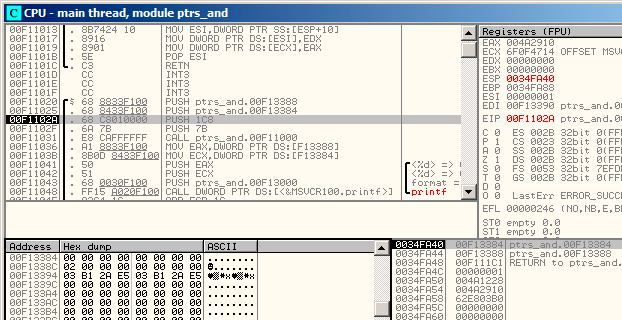
\includegraphics[scale=0.66]{patterns/061_pointers/olly_global1.png}
\caption{\olly: \IFRU{передаются адреса двух глобальных переменных в}
{global variables addresses are passing into} \ttf}
\label{fig:pointers_olly_global_1}
\end{figure}

\begin{figure}[H]
\centering
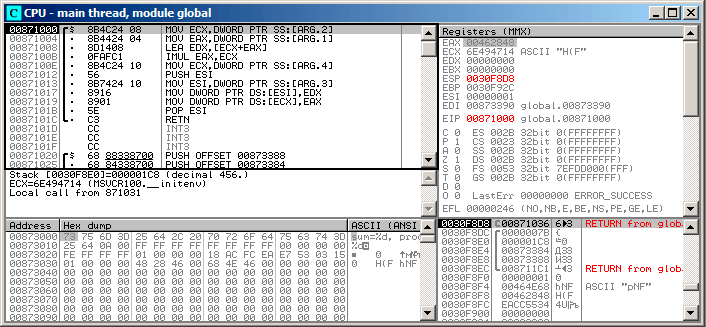
\includegraphics[scale=0.66]{patterns/061_pointers/olly_global2.png}
\caption{\olly: \IFRU{начало работы \ttf}{\ttf is started}}
\label{fig:pointers_olly_global_2}
\end{figure}

\begin{figure}[H]
\centering
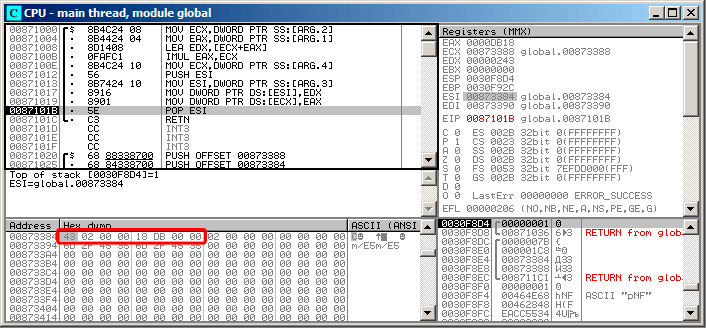
\includegraphics[scale=0.66]{patterns/061_pointers/olly_global3.png}
\caption{\olly: \ttf \IFRU{заканчивает работу}{finishes}}
\label{fig:pointers_olly_global_3}
\end{figure}

\begin{figure}[H]
\centering
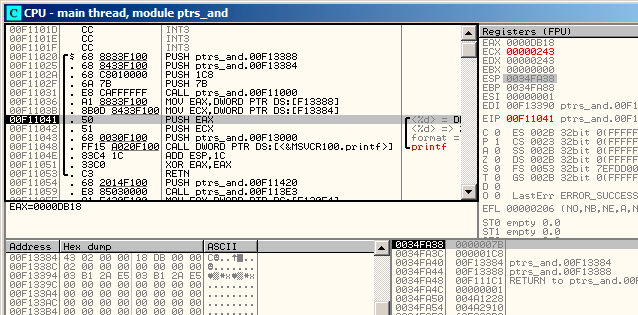
\includegraphics[scale=0.66]{patterns/061_pointers/olly_global4.png}
\caption{\olly: \IFRU{адреса глобальных переменных передаются в}
{global variables addresses are passed into} \printf}
\label{fig:pointers_olly_global_4}
\end{figure}

\begin{figure}[H]
\centering
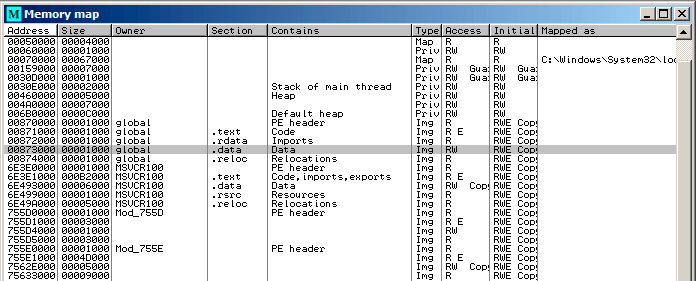
\includegraphics[scale=0.66]{patterns/061_pointers/olly_global5.png}
\caption{\olly: \IFRU{карта памяти}{memory map}}
\label{fig:pointers_olly_global_5}
\end{figure}

\subsection{\IFRU{Пример с локальными переменными}{Local variables example}}

\IFRU{Немного переделаем пример}{Let's rework our example slightly}:

\lstinputlisting[caption=\IFRU{теперь переменные локальные}
{now variables are local}]{patterns/061_pointers/local_\IFRU{ru}{en}.c}

\RU{Код ф-ции }\ttf \IFRU{не изменится}{function code will not changed}.
\IFRU{Изменится только \main}{Only \main code will}:

\lstinputlisting[caption=\Optimizing MSVC 2010 (/Ox /Ob0)]{patterns/061_pointers/local.asm}

\newcommand{\PtrsAddresses}{\TT{0x35FCF4} \AndENRU \TT{0x35FCF8}\xspace}

\IFRU{Снова посмотрим в}{Let's again take a look into} \olly.
\IFRU{Адреса локальных переменных в стеке это}{Local variable addresses in the stack are} \PtrsAddresses.
\IFRU{Видно как они заталкиваются в стек}{We see how these are pushed into the stack}: 
\figname \ref{fig:pointers_olly_stk_1}.

\IFRU{Начало работы \ttf}{\ttf is started}.
\IFRU{В стеке по адресам}{Random garbage are at} \PtrsAddresses \IFRU{пока находится случайный мусор}
{so far} \figname \ref{fig:pointers_olly_stk_2}.

\IFRU{Конец работы \ttf}{\ttf finished}.
\IFRU{В стеке по адресам \PtrsAddresses теперь значения \TT{0xDB18} \AndENRU \TT{0x243}, 
это результаты работы \ttf}
{There are \TT{0xDB18} \AndENRU \TT{0x243} now at \PtrsAddresses addresses, these values are
\ttf function result}.

\begin{figure}[H]
\centering
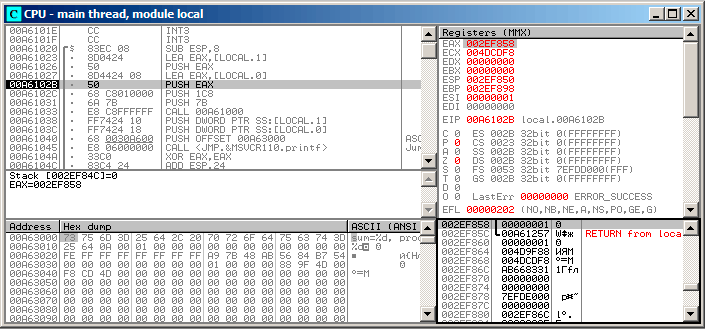
\includegraphics[scale=0.66]{patterns/061_pointers/olly_stk1.png}
\caption{\olly: \IFRU{адреса локальных переменных заталкиваются в стек}{addresses of local variables are
pushed into the stack}}
\label{fig:pointers_olly_stk_1}
\end{figure}

\begin{figure}[H]
\centering
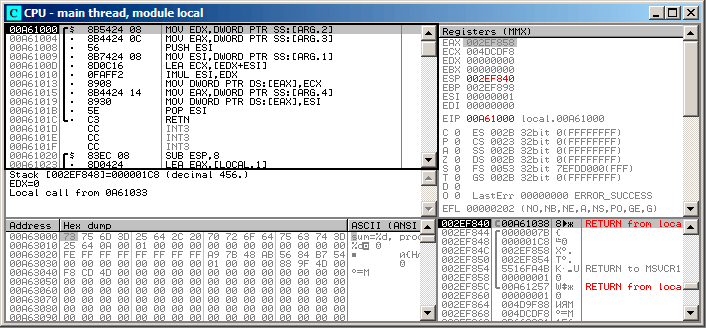
\includegraphics[scale=0.66]{patterns/061_pointers/olly_stk2.png}
\caption{\olly: \ttf \IFRU{начинает работу}{starting}}
\label{fig:pointers_olly_stk_2}
\end{figure}

\begin{figure}[H]
\centering
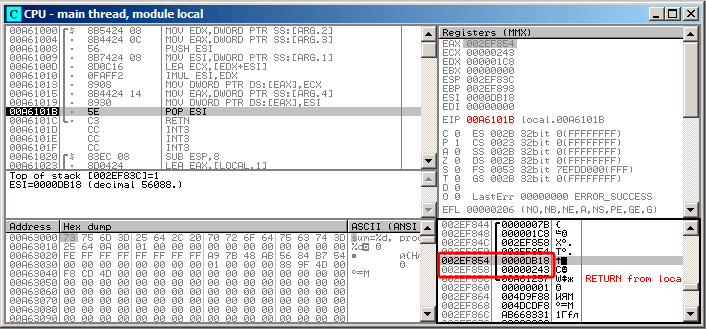
\includegraphics[scale=0.66]{patterns/061_pointers/olly_stk3.png}
\caption{\olly: \ttf \IFRU{заканчивает работу}{finished}}
\label{fig:pointers_olly_stk_3}
\end{figure}

\subsection{\IFRU{Вывод}{Conclusion}}

\IFRU{\ttf может одинаково хорошо возвращать результаты работы в любые места памяти, 
находящиеся где угодно}{\ttf can return results to any place in memory, located anywhere}.
\IFRU{В этом суть и удобство указателей}{This is essence and usefulness of pointers}.

\IFRU{Кстати,}{By the way, \Cpp} \IT{references} \IFRU{в \Cpp работают точно так же}{works just in the
same way}. \IFRU{Читайте больше об этом}{Read more about them}: (\ref{cpp_references}).


\fi
\chapter{GOTO}

\RU{Оператор GOTO считается анти-паттерном}\EN{GOTO operator considered harmful} 
\cite{Dijkstra:1968:LEG:362929.362947}, 
\RU{но тем не менее, его можно использовать в разумных пределах}
\EN{but nevertheless, can be used resonably} \cite{Knuth:1974:SPG:356635.356640}, \cite[1.3.2]{CBook}.

\RU{Вот простейший пример}\EN{Here is a simplest possible example}:

\lstinputlisting{patterns/065_GOTO/goto.c}

\RU{Вот что мы получаем в}\EN{Here is what we've got is} MSVC 2012:

\lstinputlisting[caption=MSVC 2012]{patterns/065_GOTO/MSVC_goto.asm}

\RU{Так что выражение \IT{goto} просто заменяется инструкцией \JMP, которая работает точно также:
безусловный переход в другое место.}
\EN{So the \IT{goto} statement is just replaced by \JMP instruction, which has the very same
effect: unconditional jump to another place.}

\RU{Вызов второго \printf может исполнится только при помощи человеческого вмешательства,
используя отладчик или модифицирование кода.}
\EN{The second \printf call can be executed only with the help of human intervention, 
using debugger or patching.}\\
\\
\RU{Это также может быть простым упражнением на модификацию кода.}
\EN{This also could be a simple patching exercise.}
\RU{Откроем исполняемый файл в}\EN{Let's open resulting executable in} Hiew: \figref{fig:goto_hiew1}.

\RU{Поместите курсор по адресу где}\EN{Place cursor to the address of} \JMP (\TT{0x410}), 
\RU{нажмите}\EN{press} F3 (\RU{редактирование}\EN{edit}), \RU{нажмите два нуля, так что
опкод будет}\EN{press two zeroes, so the opcode will be} \TT{EB 00}: \figref{fig:goto_hiew2}.

\RU{Второй байт опкода \JMP означает относительное смещение от перехода, 0 означает место
прямо после текущей инструкции.}
\EN{The second byte of \JMP opcode mean relative offset of jump, 0 means the point
right after current instruction.}
\RU{Теперь \JMP не будет пропускать следующий вызов \printf.}
\EN{So now \JMP will not skip second \printf call.}

\RU{Теперь нажмите F9 (запись) и выйдите.}
\EN{Now press F9 (save) and exit.}
\RU{Теперь мы запускаем исполняемый файл и видим это}\EN{Now we run executable and we see 
this}: \figref{fig:goto_result}.

\RU{Подобного же эффекта можно достичь, если заменить инструкцию \JMP на две инструкции \NOP.}
\EN{The same effect can be achieved if to replace \JMP instruction by 2 \NOP instructions.}
\RU{\NOP имеет опкод \TT{0x90} и длину в 1 байт, так что нужно 2 инструкции для замены.}
\EN{\NOP has \TT{0x90} opcode and length of 1 byte, so we need 2 instructions as replacement.}

\begin{figure}[H]
\centering
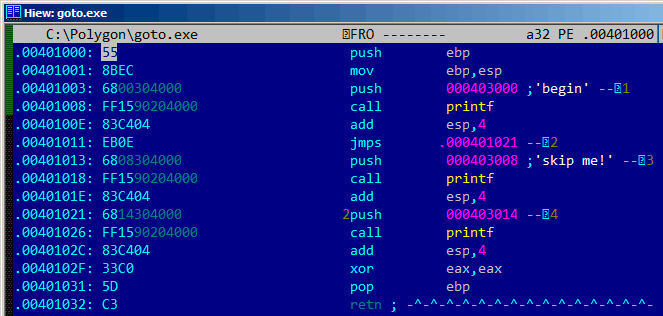
\includegraphics[scale=0.66]{patterns/065_GOTO/hiew1.png}
\caption{Hiew}
\label{fig:goto_hiew1}
\end{figure}

\begin{figure}[H]
\centering
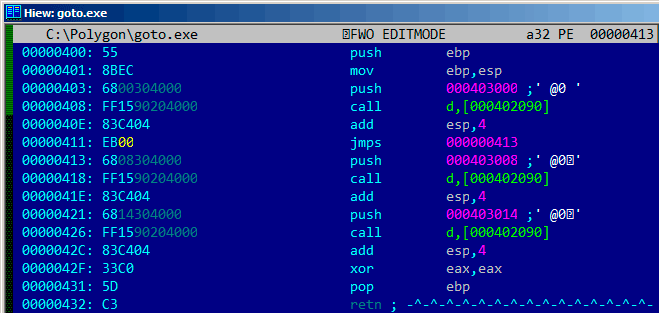
\includegraphics[scale=0.66]{patterns/065_GOTO/hiew2.png}
\caption{Hiew}
\label{fig:goto_hiew2}
\end{figure}

\begin{figure}[H]
\centering
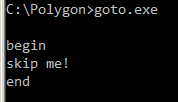
\includegraphics[scale=0.66]{patterns/065_GOTO/result.png}
\caption{\RU{Результат}\EN{Result}}
\label{fig:goto_result}
\end{figure}

\section{\RU{Мертвый код}\EN{Dead code}}

\RU{Вызов второго \printf также называется ``мертвым кодом'' (``dead code'') 
в терминах компиляторов.}
\EN{The second \printf call is also called ``dead code'' in compiler's term.}
\RU{Это значит что он никогда не будет исполнен}\EN{This mean, the code will never be executed}.
\EN{So when you compile this example with optimization, compiler removing ``dead code'' leaving
no trace of it:}
\RU{Так что если вы компилируете этот пример с оптимизацией, компилятор удаляет ``мертвый
код'' не оставляя следа:}

\lstinputlisting[caption=\Optimizing MSVC 2012]{patterns/065_GOTO/MSVC_goto_Ox.asm}

\RU{Впрочем, строку}\EN{However, compiler forgot to remove the} ``skip me!'' \RU{компилятор 
убрать забыл}\EN{string}.

\section{\Exercise}

\RU{Попробуйте добиться того же самого используя ваш любимый компилятор и отладчик.}
\EN{Try to achieve the same result using your favorite compiler and debugger.}

\chapter{\RU{Условные переходы}\EN{Conditional jumps}}
\label{sec:Jcc}
\index{\CLanguageElements!if}

% sections
\input{patterns/07_jcc/simple/main}
\input{patterns/07_jcc/abs/main}
\input{patterns/07_jcc/cond_operator/main}
\input{patterns/07_jcc/minmax/main}

\section{\Conclusion{}}

\subsection{x86}

\RU{Примерный скелет условных переходов}\EN{Here's the rough skeleton of a conditional jump}:

\lstinputlisting[caption=x86]{patterns/07_jcc/skel1.lst.\LANG}

\ifdefined\IncludeARM

\subsection{ARM}

\lstinputlisting[caption=ARM]{patterns/07_jcc/skel2.lst.\LANG}
\fi

\ifdefined\IncludeMIPS

\subsection{MIPS}

\begin{lstlisting}[caption=\RU{Проверка на ноль}\EN{Check for zero}]
BEQZ REG, label
...
\end{lstlisting}

\begin{lstlisting}[caption=\RU{Меньше ли нуля?}\EN{Check for less than zero:}]
BLTZ REG, label
...
\end{lstlisting}

\begin{lstlisting}[caption=\RU{Проверка на равенство}\EN{Check for equal values}]
BEQ REG1, REG2, label
...
\end{lstlisting}

\begin{lstlisting}[caption=\RU{Проверка на неравенство}\EN{Check for non-equal values}]
BNE REG1, REG2, label
...
\end{lstlisting}

\begin{lstlisting}[caption=\RU{Проверка на меньше, больше (знаковое)}\EN{Check for less than, greater than (signed)}]
SLT REG1, REG2, REG3
BEQ REG1, label
...
\end{lstlisting}

\begin{lstlisting}[caption=\RU{Проверка на меньше, больше (беззнаковое)}\EN{Check for less than, greater than (unsigned)}]
SLTU REG1, REG2, REG3
BEQ REG1, label
...
\end{lstlisting}
\fi

\subsection{\RU{Без инструкций перехода}\EN{Branchless}}

\index{ARM!\Instructions!MOVcc}
\index{x86!\Instructions!CMOVcc}
\index{ARM!\Instructions!CSEL}
\EN{If the body of a condition statement is very short, the conditional move instruction can be used: 
MOVcc in ARM (in ARM mode), CSEL in ARM64, CMOVcc in x86.}
\RU{Если тело условного выражения очень короткое, инструкция условного копирования может быть
использована: MOVcc в ARM (в режиме ARM), CSEL в ARM64, CMOVcc в x86.}

\ifdefined\IncludeARM
\subsubsection{ARM}

\RU{В режиме ARM, Можно использовать условные суффиксы для некоторых инструкций:}
\EN{It's possible to use conditional suffixes in ARM mode for some instructions:}

\lstinputlisting[caption=ARM (\ARMMode)]{patterns/07_jcc/skel4.lst.\LANG}

\RU{Конечно, нет никаких ограничений на количество инструкций с условными суффиксами, до тех пор
пока флаги CPU не были модифицированы одной из таких инструкций.}
\EN{Of course, there is no limit for the number of instructions with conditional code suffixes, 
as long as the CPU flags are not modified by any of them.}
% FIXME: list of such instructions or \myref{} to it

\index{ARM!\Instructions!IT}
\RU{В режиме Thumb есть инструкция IT, позволяющая дополнить следующие 4 инструкции суффиксами, задающими
условие.}
\EN{Thumb mode has the IT instruction, allowing to add conditional suffixes to the next four instructions.}
\RU{Читайте больше об этом}\EN{Read more about it}: \myref{ARM_Thumb_IT}.

\lstinputlisting[caption=ARM (\ThumbMode)]{patterns/07_jcc/skel3.lst.\LANG}
\fi

\ifdefined\IncludeExercises
\section{\Exercise}

(ARM64) \RU{Попробуйте переписать код в}\EN{Try rewriting the code in} \lstref{cond_ARM64} 
\RU{убрав все инструкции условного перехода, и используйте инструкцию \TT{CSEL}}\EN{by removing all 
conditional jump instructions and using the \TT{CSEL} instruction}.
\fi


\chapter{\SwitchCaseDefaultSectionName}
\index{\CLanguageElements!switch}

% sections
\input{patterns/08_switch/1_few/main}
\input{patterns/08_switch/2_lot/main}
\input{patterns/08_switch/3_several_cases/main}
\input{patterns/08_switch/4_fallthrough/main}

\ifdefined\IncludeExercises
\section{\Exercises}

\subsection{\Exercise \#1}
\label{exercise_switch_1}

\RU{Вполне возможно переделать пример на Си в листинге \ref{switch_lot_c} так, чтобы при компиляции
получалось даже еще меньше кода, но работать всё будет точно так же.}
\EN{It's possible to rework C example in \ref{switch_lot_c} in such way, so the compiler
will produce even smaller code, but it will work just the same.}
\RU{Попробуйте этого добиться}\EN{Try to achieve it}.

\RU{Подсказка}\EN{Hint}: \ref{exercise_solutions_switch_1}.
\fi

\chapter{\Loops}
\label{sec:loops}

% sections
\input{patterns/09_loops/simple/main}
\input{patterns/09_loops/memcpy/main}
\input{patterns/09_loops/conclusion}
\ifdefined\IncludeExercises
\input{patterns/09_loops/exercises}
\fi

\chapter{\SimpleStringsProcessings}
\index{\CStandardLibrary!strlen()}
\index{\CLanguageElements!while}

% sections
\input{patterns/10_strings/1_strlen/main}
\input{patterns/10_strings/4_trim/main}
\input{patterns/10_strings/exercises}

\chapter{\ArithOptimizations}

\RU{В целях оптимизации одна инструкция может быть заменена другой, или даже группой инструкций.}
\EN{In the pursuit of optimization, one instruction may be replaced by another, 
or even with a group of instructions.} \RU{Например}\EN{For example}, \ADD \AndENRU \SUB \RU{могут заменять друг друга}\EN{can replace each other}:
\LineENRU 18 \InENRU \lstref{neg_array_c}.

\ifx\LITE\undefined
\RU{Более того, не всегда замена тривиальна. Инструкция \LEA, несмотря на оригинальное назначение, нередко применяется для простых арифметических действий:}
\EN{For example, the \LEA instruction is often used for simple arithmetic calculations:}  \myref{sec:LEA}.

\fi

% sections
\input{patterns/11_arith_optimizations/mult}
\input{patterns/11_arith_optimizations/div}
\ifdefined\IncludeExercises
\input{patterns/11_arith_optimizations/exercises}
\fi

\ifx\LITE\undefined
\chapter{\FPUChapterName}
\label{sec:FPU}

\newcommand{\FNURLSTACK}{\footnote{\url{http://en.wikipedia.org/wiki/Stack_machine}}}
\newcommand{\FNURLFORTH}{\footnote{\url{http://en.wikipedia.org/wiki/Forth_(programming_language)}}}
\newcommand{\FNURLIEEE}{\footnote{\url{http://en.wikipedia.org/wiki/IEEE_754-2008}}}
\newcommand{\FNURLSP}{\footnote{\url{http://en.wikipedia.org/wiki/Single-precision_floating-point_format}}}
\newcommand{\FNURLDP}{\footnote{\url{http://en.wikipedia.org/wiki/Double-precision_floating-point_format}}}
\newcommand{\FNURLEP}{\footnote{\url{http://en.wikipedia.org/wiki/Extended_precision}}}

\ac{FPU}\EMDASH\RU{блок в процессоре работающий с числами с плавающей запятой.}
\EN{is a device within main \ac{CPU} specially designed to deal with floating point numbers.}\\
\\
\RU{Раньше он назывался сопроцессором. Он немного похож на программируемый калькулятор и 
стоит немного в стороне от \ac{CPU}.}
\EN{It was called coprocessor in past.
It stay aside of the main \ac{CPU} and looks like programmable calculator
in some way and.}\\
\\
\RU{Перед изучением \ac{FPU} полезно ознакомиться с тем как работают стековые машины\FNURLSTACK, 
или ознакомиться с основами языка Forth\FNURLFORTH.}
\EN{It is worth to study stack machines\FNURLSTACK{} before \ac{FPU} studying, or learn Forth language basics\FNURLFORTH.}\\
\\
\index{Intel!80486}
\index{Intel!FPU}
\RU{Интересен факт, что в свое время (до 80486) сопроцессор был отдельным чипом на материнской плате, 
и вследствие его высокой цены, он стоял не всегда. Его можно было докупить отдельно и поставить}
\EN{It is interesting to know that in past (before 80486 CPU) coprocessor was a separate chip 
and it was not always settled on motherboard. It was possible to buy it separately and install}
\footnote{\RU{Например, Джон Кармак использовал в своей игре Doom числа с фиксированной запятой, хранящиеся
в обычных 32-битных \ac{GPR} (16 бит на целую часть и 16 на дробную),
чтобы Doom работал на 32-битных компьютерах без FPU, т.е., 80386 и 80486 SX}
\EN{For example, John Carmack used fixed-point arithmetic values in his Doom video game, stored in 
32-bit \ac{GPR} registers (16 bit for intergral part and another 16 bit for fractional part), so the Doom
could work on 32-bit computer without FPU, i.e., 80386 and 80486 SX}}.\\
\\
\RU{Начиная с процессора 80486 DX, FPU уже всегда входит в его состав.}
\EN{Starting at 80486 DX CPU, FPU is always present in it.}\\
\\
\index{x86!\Instructions!FWAIT}
\RU{Этот факт может напоминать такой рудимент, как наличие инструкции вроде \TT{FWAIT}, 
которая заставляет
\ac{CPU} ожидать, пока \ac{FPU} закончит работу}\EN{\TT{FWAIT} instruction may remind us that fact---it
switches \ac{CPU} to waiting state, so it can wait until \ac{FPU} finishes its work}.
\RU{Другой рудимент, это тот факт что опкоды \ac{FPU}-инструкций начинаются с т.н. ``escape''-опкодов 
(\TT{D8..DF}), т.е., опкоды, передающиеся в \ac{FPU}}\EN{Another rudiment is the fact that 
\ac{FPU}-instruction 
opcodes are started with so called ``escape''-opcodes (\TT{D8..DF}), i.e., opcodes passed into \ac{FPU}}. \\
\\
\index{IEEE 754}
\label{FPU_is_stack}
\RU{FPU имеет стек из восьми 80-битных регистров, каждый может содержать число в формате IEEE 754\FNURLIEEE.}
\EN{FPU has a stack capable to hold 8 80-bit registers, each register can hold a number 
in IEEE 754\FNURLIEEE format.}\\
\\
\index{float}
\index{double}
\RU{В \CCpp имеются два типа для работы с числами с плавающей запятой, 
это \Tfloat (\IT{число одинарной точности}\FNURLSP, 32 бита)
\footnote{Формат представления float-чисел затрагивается в разделе 
\IT{\WorkingWithFloatAsWithStructSubSubSectionName}~(\ref{sec:floatasstruct}).}
и \Tdouble (\IT{число двойной точности}\FNURLDP, 64 бита).}
\EN{\CCpp language offer at least two floating number types, \Tfloat (\IT{single-precision}\FNURLSP, 32 bits)
\footnote{single precision float numbers format is also addressed in 
the \IT{\WorkingWithFloatAsWithStructSubSubSectionName}~(\ref{sec:floatasstruct}) section}
and \Tdouble (\IT{double-precision}\FNURLDP, 64 bits).}\\
\\
\index{long double}
\RU{GCC также поддерживает тип \IT{long double} (\IT{extended precision}\FNURLEP, 80 бит), но MSVC ~--- нет.}
\EN{GCC also supports \IT{long double} type (\IT{extended precision}\FNURLEP, 80 bit) but MSVC is not.}\\
\\
\RU{Не смотря на то что \Tfloat занимает столько же места сколько \Tint на 32-битной архитектуре, 
представление чисел, разумеется, совершенно другое.}
\EN{\Tfloat type requires the same number of bits as \Tint type in 32-bit environment, 
but number representation is completely different.}\\
\\
\RU{Число с плавающей точкой состоит из знака, мантиссы\footnote{\IT{significand} или \IT{fraction} 
в англоязычной литературе} и экспоненты.}
\EN{Number consisting of sign, significand (also called \IT{fraction}) and exponent.}\\
\\
\RU{Функция, имеющая \Tfloat или \Tdouble среди аргументов, получает эти значения через стек. 
Если функция возвращает \Tfloat или \Tdouble, она оставляет значение в регистре \ST{0} ~--- то есть, 
на вершине FPU-стека.}
\EN{Function having \Tfloat or \Tdouble among argument list is getting 
the value via stack. 
If function returns \Tfloat or \Tdouble value,
it leaves the value in the \ST{0}
register~---at top of FPU stack.}

\input{patterns/12_FPU/1_simple/main}
\input{patterns/12_FPU/2_passing_floats/main}
\input{patterns/12_FPU/3_comparison/main}

\section{x64}

\RU{О том как происходит работа с числами с плавающей запятой в x86-64, читайте здесь: 
\ref{floating_SIMD}.}
\EN{Read more here\ref{floating_SIMD} about how float point numbers are processed in x86-64.}

% sections
\input{patterns/12_FPU/exercises}

\fi
\chapter{\Arrays}
\label{arrays}

\RU{Массив это просто набор переменных в памяти, 
обязательно лежащих рядом и обязательно одного типа%
\footnote{\ac{AKA} \q{гомогенный контейнер}}.}
\EN{An array is just a set of variables in memory 
that lie next to each other and that have the same type%
\footnote{\ac{AKA} \q{homogeneous container}}.}

% sections
\input{patterns/13_arrays/1_simple/main}
\input{patterns/13_arrays/2_BO/main}
\ifx\LITE\undefined
\input{patterns/13_arrays/3_BO_protection/main}
\fi
\input{patterns/13_arrays/4_one_more_thing/main}
\input{patterns/13_arrays/45_month_1D/main}
\input{patterns/13_arrays/5_multidimensional/main}
\ifx\LITE\undefined
\input{patterns/13_arrays/55_month_2D/main}
\fi
\input{patterns/13_arrays/conclusion}
\ifdefined\IncludeExercises
\input{patterns/13_arrays/exercises}
\fi

\section{\IFRU{Битовые поля}{Bit fields}}
\label{sec:bitfields}

\IFRU{Немало функций задают различные флаги в аргументах при помощи битовых 
полей\footnote{bit fields в англоязычной литературе}.}
{A lot of functions defining input flags in arguments using bit fields.}
\index{\CLanguageElements!C99!bool}
\IFRU{Наверное, вместо этого, можно было бы использовать набор переменных типа \IT{bool}, но это было бы 
не очень экономно.}
{Of course, it could be substituted by \IT{bool}-typed variables set, but it is not frugally.}

\input{patterns/14_bitfields/check}
\input{patterns/14_bitfields/set_reset}
\input{patterns/14_bitfields/shifts}
\input{patterns/14_bitfields/CRC32}


\chapter[\RU{Линейный конгруэнтный генератор}\EN{Linear congruential generator}]
{\RU{Линейный конгруэнтный генератор как генератор псевдослучайных чисел}\EN{Linear congruential generator as pseudorandom number generator}}
\index{\CStandardLibrary!rand()}
\label{LCG_simple}

\RU{Линейный конгруэнтный генератор, пожалуй, самый простой способ генерировать псевдослучайные числа.}
\EN{The linear congruential generator is probably the simplest possible way to generate random numbers.}
\RU{Он не в почете в наше время\footnote{Вихрь Мерсенна куда лучше}, но он настолько прост
(только одно умножение, одно сложение и одна операция \q{И}),
что мы можем использовать его в качестве примера.}
\EN{It's not in favour in modern times\footnote{Mersenne twister is better}, but it's so simple 
(just one multiplication, one addition and one AND operation), 
we can use it as an example.}

\lstinputlisting{patterns/145_LCG/rand.c.\LANG}

\RU{Здесь две функции: одна используется для инициализации внутреннего состояния, а вторая
вызывается собственно для генерации псевдослучайных чисел.}
\EN{There are two functions: the first one is used to initialize the internal state, and the second one is called
to generate pseudorandom numbers.}

\RU{Мы видим что в алгоритме применяются две константы}\EN{We see that two constants are used in the algorithm}.
\RU{Они взяты из}\EN{They are taken from} \cite{Numerical}.
\RU{Определим их используя выражение \CCpp \TT{\#define}. Это макрос.}
\EN{Let's define them using a \TT{\#define} \CCpp statement. It's a macro.}
\RU{Разница между макросом в \CCpp и константой в том, что все макросы заменяются на значения препроцессором
\CCpp и они не занимают места в памяти как переменные.}
\EN{The difference between a \CCpp macro and a constant is that all macros are replaced 
with their value by \CCpp preprocessor,
and they don't take any memory, unlike variables.}
\RU{А константы, напротив, это переменные только для чтения.}
\EN{In contrast, a constant is a read-only variable.}
\RU{Можно взять указатель (или адрес) переменной-константы, но это невозможно сделать с макросом.}
\EN{It's possible to take a pointer (or address) of a constant variable, but impossible to do so with a macro.}

\RU{Последняя операция \q{И} нужна, потому что согласно стандарту Си \TT{my\_rand()} должна возвращать значение в пределах
0..32767.}
\EN{The last AND operation is needed because by C-standard \TT{my\_rand()} has to return a value in 
the 0..32767 range.}
\RU{Если вы хотите получать 32-битные псевдослучайные значения, просто уберите последнюю операцию \q{И}.}
\EN{If you want to get 32-bit pseudorandom values, just omit the last AND operation.}

\section{x86}

\lstinputlisting[caption=\Optimizing MSVC 2013]{patterns/145_LCG/rand_MSVC_2013_x86_Ox.asm}

\RU{Вот мы это и видим: обе константы встроены в код.}
\EN{Here we see it: both constants are embedded into the code.}
\RU{Память для них не выделяется.}\EN{There is no memory allocated for them.}
\RU{Функция \TT{my\_srand()} просто копирует входное значение во внутреннюю переменную \TT{rand\_state}.}
\EN{The \TT{my\_srand()} function just copies its input value into the internal \TT{rand\_state} variable.}

\RU{\TT{my\_rand()} берет её, вычисляет следующее состояние \TT{rand\_state}, 
обрезает его и оставляет в регистре EAX.}
\EN{\TT{my\_rand()} takes it, calculates the next \TT{rand\_state}, cuts it and leaves it in the EAX register.}

\RU{Неоптимизированная версия побольше}\EN{The non-optimized version is more verbose}:

\lstinputlisting[caption=\NonOptimizing MSVC 2013]{patterns/145_LCG/rand_MSVC_2013_x86.asm}

\section{x64}

\RU{Версия для x64 почти такая же, и использует 32-битные регистры вместо 64-битных
(потому что мы работаем здесь с переменными типа \Tint).}
\EN{The x64 version is mostly the same and uses 32-bit registers instead of 64-bit ones 
(because we are working with \Tint values here).}
\RU{Но функция \TT{my\_srand()} берет входной аргумент из регистра \ECX, а не из стека:}
\EN{But \TT{my\_srand()} takes its input argument from the \ECX register rather than from stack:}

\lstinputlisting[caption=\Optimizing MSVC 2013 x64]{patterns/145_LCG/rand_MSVC_2013_x64_Ox.asm.\LANG}

\ifdefined\IncludeGCC
\RU{GCC делает почти такой же код}\EN{GCC compiler generates mostly the same code}.
\fi

\ifdefined\IncludeARM
\section{32-bit ARM}

\lstinputlisting[caption=\OptimizingKeilVI (\ARMMode)]{patterns/145_LCG/rand.s_Keil_ARM_O3.s.\LANG}

\ifdefined\RUSSIAN
В ARM инструкцию невозможно встроить 32-битную константу, так что Keil-у приходится размещать их отдельно и дополнительно загружать.
Вот еще что интересно: константу 0x7FFF также нельзя встроить.
Поэтому Keil сдвигает \TT{rand\_state} влево на 17 бит и затем сдвигает вправо на 17 бит.
Это аналогично \CCpp{}-выражению $(rand\_state \ll 17) \gg 17$.
Выглядит как бессмысленная операция, но тем не менее, что она делает это очищает старшие 17 бит, оставляя младшие 15 бит нетронутыми, и это наша цель, в конце концов. \\
\\
\Optimizing Keil для режима Thumb делает почти такой же код.
\fi % RUSSIAN

\ifdefined\ENGLISH
It's not possible to embed 32-bit constants into ARM instructions, so Keil has to place them externally and load them additionally.
One interesting thing is that it's not possible to embed the 0x7FFF constant as well.
So what Keil does is shifting \TT{rand\_state} left by 17 bits and then shifting it right by 17 bits.
This is analogous to the $(rand\_state \ll 17) \gg 17$ statement in \CCpp.
It seems to be useless operation, but what it does is clearing the high 17 bits, leaving the low 15 bits intact, and that's our goal after all. \\
\\
\Optimizing Keil for Thumb mode generates mostly the same code.
\fi % ENGLISH

\fi % IncludeARM

\ifdefined\IncludeMIPS
\input{patterns/145_LCG/MIPS}
\fi

\ifx\LITE\undefined
\section{\RU{Версия этого примера для многопоточной среды}\EN{Thread-safe version of the example}}

\RU{Версия примера для многопоточной среды будет рассмотрена позже}%
\EN{The thread-safe version of the example is to be demonstrated later}: \myref{LCG_TLS}.
\fi

\chapterold{\StructuresChapterName}

\RU{В принципе, структура в \CCpp это, с некоторыми допущениями, просто всегда лежащий рядом, 
и в той же последовательности, набор переменных, не обязательно одного типа
\footnote{\ac{AKA} \q{гетерогенный контейнер}}.}
\EN{A \CCpp structure, with some assumptions, is just a set of variables, always stored
in memory together, not necessary of the same type
\footnote{\ac{AKA} \q{heterogeneous container}}.}

% sections
\EN{\input{patterns/15_structs/1_systemtime/main_EN.tex}}
\RU{\input{patterns/15_structs/1_systemtime/main_RU.tex}}
\input{patterns/15_structs/2_using_malloc/main.tex}
\input{patterns/15_structs/3_tm_linux/main.tex}
\EN{\input{patterns/15_structs/4_packing/main_EN.tex}}
\RU{\input{patterns/15_structs/4_packing/main_RU.tex}}
\EN{\input{patterns/15_structs/5_nested/main_EN.tex}}
\RU{\input{patterns/15_structs/5_nested/main_RU.tex}}
\input{patterns/15_structs/6_bitfields/main.tex}
\input{patterns/15_structs/exercises}


\ifx\LITE\undefined
\chapter{\RU{Объединения (union)}\EN{Unions}}

\input{patterns/17_unions/FPU_PRNG_example}

\newcommand{\comp}{\TT{comp()}\xspace}
\chapter{\RU{Указатели на функции}\EN{Pointers to functions}}
\label{sec:pointerstofunctions}

\index{\CLanguageElements!\Pointers}
\RU{Указатель на функцию, в целом, как и любой другой указатель, просто адрес указывающий на начало функции 
в сегменте кода.}
\EN{Pointer to function, as any other pointer, is just an address of function beginning in its code segment.}

\index{Callbacks}
\RU{Это применяется часто в т.н. callback-ах}\EN{It is often used in callbacks}
\footnote{\url{http://en.wikipedia.org/wiki/Callback_(computer_science)}}.

\RU{Известные примеры:}\EN{Well-known examples are:}

\begin{itemize}
\item
\qsort\footnote{\url{http://en.wikipedia.org/wiki/Qsort_(C_standard_library)}},
{\TT{atexit()}}\footnote{\url{http://www.opengroup.org/onlinepubs/009695399/functions/atexit.html}} \RU{из стандартной библиотеки Си}\EN{from the standard C library}; 
\item
\RU{сигналы в *NIX ОС}\EN{signals in *NIX OS}\footnote{\url{http://en.wikipedia.org/wiki/Signal.h}};
\item
\RU{запуск тредов}\EN{thread starting}: \TT{CreateThread()} (win32), \TT{pthread\_create()} (POSIX);
\item
\RU{множество функций win32, например}\EN{a lot of win32 functions, e.g.} \TT{EnumChildWindows()}\footnote{\url{http://msdn.microsoft.com/en-us/library/ms633494(VS.85).aspx}}.
\end{itemize}

\index{\CStandardLibrary!qsort()}
\RU{Итак, функция \qsort это реализация алгоритма ``быстрой сортировки''. 
Функция может сортировать что угодно, 
любые типы данных, но при условии, что вы имеете функцию сравнения двух элементов данных и 
\qsort может вызывать её.}
\EN{So, \qsort function is a \CCpp standard library quicksort implementation. The functions is able to sort
anything, any types of data, if you have a function for two elements comparison and \qsort is able
to call it.}

\RU{Эта функция сравнения может определяться так:}\EN{The comparison function can be defined as:}

\begin{lstlisting}
int (*compare)(const void *, const void *)
\end{lstlisting}

\RU{Воспользуемся немного модифицированным примером, который я нашел вот}
\EN{Let's use slightly modified example I found} \href{http://cplus.about.com/od/learningc/ss/pointers2_8.htm}
{\RU{здесь}\EN{here}}:

\lstinputlisting[numbers=left,label=qsort_c_src]{patterns/18_pointers_to_functions/17_1.c}

\section{MSVC}

\RU{Компилируем в MSVC 2010 (я убрал некоторые части для краткости) с опцией \Ox}
\EN{Let's compile it in MSVC 2010 (I omitted some parts for the sake of brevity) with \Ox option}:

\lstinputlisting[caption=\Optimizing MSVC 2010: /Ox /GS- /MD]{patterns/18_pointers_to_functions/17_2_msvc_Ox.asm}

\RU{Ничего особо удивительного здесь мы не видим. В качестве четвертого аргумента, 
в \qsort просто передается адрес метки \TT{\_comp}, где собственно и располагается функция \comp.}
\EN{Nothing surprising so far.
As a fourth argument, an address of label \TT{\_comp} is passed, that is just a place
where function \comp located.}

\RU{Как \qsort вызывает её?}\EN{How \qsort calling it?}

\index{Windows!MSVCR80.DLL}
\RU{Посмотрим в MSVCR80.DLL (эта DLL куда в MSVC вынесены функции из стандартных библиотек Си):}
\EN{Let's take a look into this function located in MSVCR80.DLL (a MSVC DLL module with C standard library functions):}

\lstinputlisting[caption=MSVCR80.DLL]{patterns/18_pointers_to_functions/17_3_MSVCR.lst}

\TT{comp}\EMDASH{}\RU{это четвертый аргумент функции. 
Здесь просто передается управление по адресу указанному в \TT{comp}. 
Перед этим подготавливается два аргумента для функции \comp. 
Далее, проверяется результат её выполнения.}
\EN{is fourth function argument.
Here the control is just passed to the address in the \TT{comp} argument.
Before it, two arguments prepared for \comp. Its result is checked after its execution.}

\RU{Вот почему использование указателей на функции ~--- это опасно. 
Во-первых, если вызвать \qsort с неправильным указателем на функцию, 
то \qsort, дойдя до этого вызова, может передать управление неизвестно куда, 
процесс упадет, и эту ошибку можно будет найти не сразу.}
\EN{That's why it is dangerous to use pointers to functions.
First of all, if you call \qsort with incorrect pointer to function, \qsort may pass control
to incorrect point, a process may crash and this bug will be hard to find.}

\RU{Во-вторых, типизация callback-функции должна строго соблюдаться, 
вызов не той функции с не теми аргументами не того типа, 
может привести к плачевным результатам, 
хотя падение процесса это и не проблема, проблема ~--- это найти ошибку, ведь компилятор 
на стадии компиляции может вас и не предупредить о потенциальных неприятностях.}
\EN{Second reason is the callback function types must comply strictly, calling wrong function
with wrong arguments of wrong types may lead to serious problems, however, process crashing is not a 
big problem~---big problem is to determine a reason of crashing~---because compiler may be 
silent about potential trouble while compiling.}

\subsection{MSVC + \olly}
\index{\olly}

\RU{Загрузим наш пример в \olly и установим брякпойнт на ф-ции \comp}
\EN{Let's load our example into \olly and set breakpoint on \comp function}.

\RU{Как значения сравниваются, мы можем увидеть во время самого первого вызова \comp}
\EN{How values are compared we can see at the very first \comp call}: \figname \ref{fig:qsort_olly1}.
\RU{Для удобства, }\olly \RU{показывает сравниваемые значения в окне под окном кода}
\EN{shows compared values in the window under code window, for convenience}.
\RU{Мы можем так же увидеть что}\EN{We can also see that the} \ac{SP} \RU{указывает на}\EN{pointing to} 
\ac{RA} \RU{где находится место в ф-ции}\EN{where the place in} 
\qsort \EN{function is }(\RU{на самом деле, находится в}\EN{actually located in} \TT{MSVCR100.DLL}).

\RU{Трассируя}\EN{By tracing} (F8) \RU{до инструкции}\EN{until} \TT{RETN} 
\RU{и нажав F8 еще один раз, мы возвращаемся в ф-цию}\EN{instruction, and pressing F8 one more time, 
we returning into} \qsort\EN{ function}: \figname \ref{fig:qsort_olly2}.
\RU{Это был вызов ф-ции сравнения}\EN{That was a call to comparison function}.

\RU{Вот также скриншот момента второго вызова ф-ции}\EN{Here is also screenshot of the moment of the 
second call of} \comp\EMDASH{}\RU{теперь сравниваемые значения другие}
\EN{now values to be compared are different}:
\figname \ref{fig:qsort_olly3}.

\begin{figure}[H]
\centering
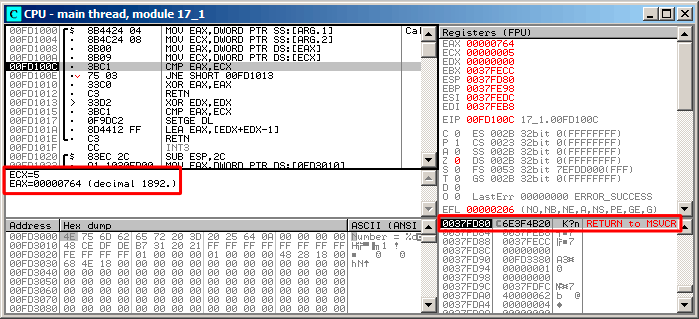
\includegraphics[scale=\FigScale]{patterns/18_pointers_to_functions/olly1.png}
\caption{\olly: \RU{первый вызов}\EN{first call of} \comp}
\label{fig:qsort_olly1}
\end{figure}

\begin{figure}[H]
\centering
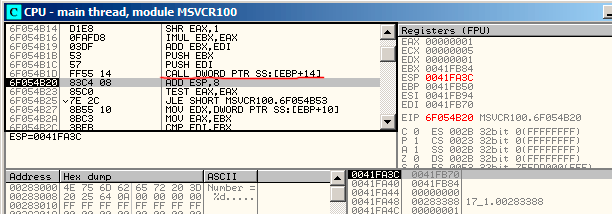
\includegraphics[scale=\FigScale]{patterns/18_pointers_to_functions/olly2.png}
\caption{\olly: \RU{код в}\EN{the code in} \qsort \RU{сразу после вызова}\EN{right after} \comp\EN{ call}}
\label{fig:qsort_olly2}
\end{figure}

\begin{figure}[H]
\centering
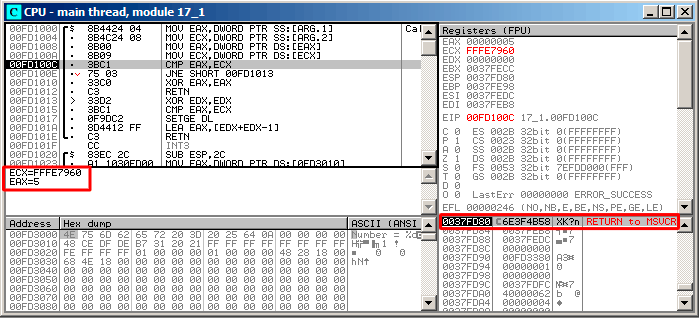
\includegraphics[scale=\FigScale]{patterns/18_pointers_to_functions/olly3.png}
\caption{\olly: \RU{второй вызов}\EN{second call of} \comp}
\label{fig:qsort_olly3}
\end{figure}

\subsection{MSVC + tracer}
\index{tracer}

\RU{Посмотрим, какие пары сравниваются}\EN{Let's also see, which pairs are compared}.
\RU{Эти 10 чисел будут сортироваться}\EN{These 10 numbers are being sorted}: 
1892, 45, 200, -98, 4087, 5, -12345, 1087, 88, -100000.

\RU{Я нашел адрес первой инструкции}\EN{I found the address of the first} \CMP 
\RU{в}\EN{instruction in} \comp, \RU{и это}\EN{it is} \TT{0x0040100C} 
\RU{и я ставлю брякпойнт на нем}\EN{and I'm setting breakpoint on it}:

\begin{lstlisting}
tracer.exe -l:17_1.exe bpx=17_1.exe!0x0040100C
\end{lstlisting}

\RU{Получаю информацию о регистрах на брякпойнте}
\EN{I'm getting information about registers at breakpoint}:

\begin{lstlisting}
PID=4336|New process 17_1.exe
(0) 17_1.exe!0x40100c
EAX=0x00000764 EBX=0x0051f7c8 ECX=0x00000005 EDX=0x00000000
ESI=0x0051f7d8 EDI=0x0051f7b4 EBP=0x0051f794 ESP=0x0051f67c
EIP=0x0028100c
FLAGS=IF
(0) 17_1.exe!0x40100c
EAX=0x00000005 EBX=0x0051f7c8 ECX=0xfffe7960 EDX=0x00000000
ESI=0x0051f7d8 EDI=0x0051f7b4 EBP=0x0051f794 ESP=0x0051f67c
EIP=0x0028100c
FLAGS=PF ZF IF
(0) 17_1.exe!0x40100c
EAX=0x00000764 EBX=0x0051f7c8 ECX=0x00000005 EDX=0x00000000
ESI=0x0051f7d8 EDI=0x0051f7b4 EBP=0x0051f794 ESP=0x0051f67c
EIP=0x0028100c
FLAGS=CF PF ZF IF
...
\end{lstlisting}

\RU{Я отфильтровал}\EN{I filtered out} \TT{EAX} \AndENRU \TT{ECX} \RU{и получил}\EN{and got}:

\begin{lstlisting}
EAX=0x00000764 ECX=0x00000005
EAX=0x00000005 ECX=0xfffe7960
EAX=0x00000764 ECX=0x00000005
EAX=0x0000002d ECX=0x00000005
EAX=0x00000058 ECX=0x00000005
EAX=0x0000043f ECX=0x00000005
EAX=0xffffcfc7 ECX=0x00000005
EAX=0x000000c8 ECX=0x00000005
EAX=0xffffff9e ECX=0x00000005
EAX=0x00000ff7 ECX=0x00000005
EAX=0x00000ff7 ECX=0x00000005
EAX=0xffffff9e ECX=0x00000005
EAX=0xffffff9e ECX=0x00000005
EAX=0xffffcfc7 ECX=0xfffe7960
EAX=0x00000005 ECX=0xffffcfc7
EAX=0xffffff9e ECX=0x00000005
EAX=0xffffcfc7 ECX=0xfffe7960
EAX=0xffffff9e ECX=0xffffcfc7
EAX=0xffffcfc7 ECX=0xfffe7960
EAX=0x000000c8 ECX=0x00000ff7
EAX=0x0000002d ECX=0x00000ff7
EAX=0x0000043f ECX=0x00000ff7
EAX=0x00000058 ECX=0x00000ff7
EAX=0x00000764 ECX=0x00000ff7
EAX=0x000000c8 ECX=0x00000764
EAX=0x0000002d ECX=0x00000764
EAX=0x0000043f ECX=0x00000764
EAX=0x00000058 ECX=0x00000764
EAX=0x000000c8 ECX=0x00000058
EAX=0x0000002d ECX=0x000000c8
EAX=0x0000043f ECX=0x000000c8
EAX=0x000000c8 ECX=0x00000058
EAX=0x0000002d ECX=0x000000c8
EAX=0x0000002d ECX=0x00000058
\end{lstlisting}

\RU{Это}\EN{That's} 34 \RU{пары}\EN{pairs}.
\RU{Следовательно, алгоритму быстрой сортировки нужно 34 операции сравнения для сортировки этих
10-и чисел}\EN{Therefore, quick sort algorithm needs 34 comparison operations for sorting these 10 numbers}.

\subsection{MSVC + tracer (code coverage)}
\index{tracer}

\RU{Но можно также и воспользоваться возможностью tracer накапливать все возможные состояния регистров
и показать их в \IDA}\EN{We can also use tracer's feature to collect all possible register's values
and show them in \IDA}.

\RU{Трассируем все инструкции в ф-ции \comp}\EN{Let's trace all instructions in \comp function}:

\begin{lstlisting}
tracer.exe -l:17_1.exe bpf=17_1.exe!0x00401000,trace:cc
\end{lstlisting}

\RU{Получем .idc-скрипт для загрузки в \IDA и загружаем его}
\EN{We getting .idc-script for loading into \IDA and load it}: \figname \ref{fig:qsort_tracer_cc}.

\RU{Имя этой ф-ции (PtFuncCompare) дала \IDA}\EN{\IDA gave the function name (PtFuncCompare)}
\EMDASH{}\RU{видимо, потому что видит что указатель на эту ф-цию передается в \qsort}\EN{it seems,
because \IDA sees that pointer to this function is passed into \qsort}.

\RU{Мы видим что указатели $a$ и $b$ указывают на разные места внутри массива, 
но шаг между указателями --- 4, что логично, ведь в массиве хранятся 32-битные значения}
\EN{We see that $a$ and $b$ pointers are points to various places in array, but step between
points is 4---indeed, 32-bit values are stored in the array}.

\RU{Видно что инструкции по адресам}\EN{We see that the instructions at} \TT{0x401010} \AndENRU 
\TT{0x401012} \RU{никогда не исполнялись}\EN{was never executed} 
(\RU{они и остались белыми}\EN{so they leaved as white}): 
\RU{действительно, ф-ция}\EN{indeed,} \comp \RU{никогда не возвращала 0,
потому что в массиве нет одинаковых элементов}\EN{was never returned 0, because there no equal elements}.

\begin{figure}[H]
\centering
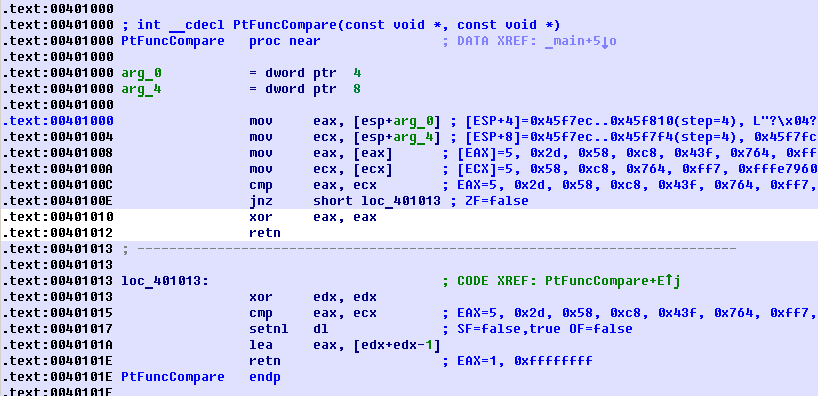
\includegraphics[scale=\FigScale]{patterns/18_pointers_to_functions/tracer_cc.png}
\caption{tracer \AndENRU IDA. N.B.: 
\RU{некоторые значения обрезаны справа}\EN{some values are cutted at right}}
\label{fig:qsort_tracer_cc}
\end{figure}

\section{GCC}

\RU{Не слишком большая разница}\EN{Not a big difference}:

\begin{lstlisting}[caption=GCC]
                lea     eax, [esp+40h+var_28]
                mov     [esp+40h+var_40], eax
                mov     [esp+40h+var_28], 764h
                mov     [esp+40h+var_24], 2Dh
                mov     [esp+40h+var_20], 0C8h
                mov     [esp+40h+var_1C], 0FFFFFF9Eh
                mov     [esp+40h+var_18], 0FF7h
                mov     [esp+40h+var_14], 5
                mov     [esp+40h+var_10], 0FFFFCFC7h
                mov     [esp+40h+var_C], 43Fh
                mov     [esp+40h+var_8], 58h
                mov     [esp+40h+var_4], 0FFFE7960h
                mov     [esp+40h+var_34], offset comp
                mov     [esp+40h+var_38], 4
                mov     [esp+40h+var_3C], 0Ah
                call    _qsort
\end{lstlisting}

\RU{Функция \comp}\EN{\comp function}:

\begin{lstlisting}
                public comp
comp            proc near

arg_0           = dword ptr  8
arg_4           = dword ptr  0Ch

                push    ebp
                mov     ebp, esp
                mov     eax, [ebp+arg_4]
                mov     ecx, [ebp+arg_0]
                mov     edx, [eax]
                xor     eax, eax
                cmp     [ecx], edx
                jnz     short loc_8048458
                pop     ebp
                retn
loc_8048458:
                setnl   al
                movzx   eax, al
                lea     eax, [eax+eax-1]
                pop     ebp
                retn
comp            endp
\end{lstlisting}

\index{Linux!libc.so.6}
\RU{Реализация \qsort находится в \TT{libc.so.6}, и представляет собой просто wrapper
\footnote{понятие близкое к \gls{thunk function}} для \TT{qsort\_r()}.}
\EN{\qsort implementation is located in the \TT{libc.so.6} and it is in fact just a wrapper
\footnote{a concept like \gls{thunk function}} for \TT{qsort\_r()}.}

\RU{Она, в свою очередь, вызывает \TT{quicksort()}, где есть вызовы определенной нами функции через 
переданный указатель:}
\EN{It will call then \TT{quicksort()}, where our defined function will be called via passed pointer:}


\begin{lstlisting}[caption=
(\RU{файл libc.so.6, версия glibc}\EN{file libc.so.6, glibc version}\EMDASH{}2.10.1)]

.text:0002DDF6                 mov     edx, [ebp+arg_10]
.text:0002DDF9                 mov     [esp+4], esi
.text:0002DDFD                 mov     [esp], edi
.text:0002DE00                 mov     [esp+8], edx
.text:0002DE04                 call    [ebp+arg_C]
...
\end{lstlisting}

\subsection{GCC + GDB (\RU{с исходными кодами}\EN{with source code})}
\index{GDB}

\RU{Очевидно, у нас есть исходный код нашего примера на Си (\ref{qsort_c_src}), 
так что мы можем установить брякпойнт (\TT{b}) на
номере строки}\EN{Obviously, we have a C-source code of our example (\ref{qsort_c_src}), 
so we can set breakpoint (\TT{b}) on line number}
(\RU{11-й --- это номер строки где происходит первое сравнение}\EN{11th---the line where 
first comparison is occurred}).
\RU{Нам также нужно скомпилировать наш пример с ключом \TT{-g}, чтобы в исполняемом файле была
полная отладочная информация}\EN{We also need to compile example with debugging information 
included (\TT{-g}), so the table
with addresses and corresponding line numbers is present}.
\RU{Мы можем так же выводить значения используя имена переменных}
\EN{We can also print values by variable name} (\TT{p}):
\RU{отладочная информация также содержит информацию о том, в каком регистре и/или элементе локального
стека находится какая переменная}\EN{debugging information also has information about which register and/or 
local stack element contain which variable}.

\index{Glibc}
\RU{Мы можем также увидеть стек}\EN{We can also see stack} (\TT{bt}) 
\RU{и обнаружить что в Glibc используется какая-то вспомогательная ф-ция с именем}
\EN{and find out that there are some intermediate function} 
\TT{msort\_with\_tmp()}\EN{ used in Glibc}.

\lstinputlisting[caption=GDB\RU{-сессия}\EN{ session}]{patterns/18_pointers_to_functions/GDB_source.txt}

\subsection{GCC + GDB (\RU{без исходных кодов}\EN{no source code})}
\index{GDB}

\RU{Но часто никаких исходных кодов нет вообще, так что мы можем дизассемблировать ф-цию \comp}
\EN{But often there are no source code at all, so we can disassemble \comp function} (\TT{disas}), 
\RU{найти самую первую инструкцию \CMP и установить брякпойнт}\EN{find the very first
\CMP instruction and set breakpoint} (\TT{b}) \RU{по этому адресу}\EN{at that address}.
\RU{На каждом брякпойнте мы будем видеть содержимое регистров}
\EN{At each breakpoint, we will dump all register contents} (\TT{info registers}).
\RU{Информация из стека так же доступна}\EN{Stack information is also available} (\TT{bt}), 
\RU{но частичная: здесь нет номеров строк для ф-ции \comp}
\EN{but partial: there are no line number information for \comp function}.

\lstinputlisting[caption=GDB\RU{-сессия}\EN{ session}]{patterns/18_pointers_to_functions/GDB_no_source.txt}


\fi
\ifdefined\ENGLISH
\section{64-bit values in 32-bit environment}
\label{sec:64bit_in_32_env}

In a 32-bit environment, \ac{GPR}'s are 32-bit, so 64-bit values are stored and passed as 32-bit value pairs
\footnote{By the way, 32-bit values are passed as pairs in 16-bit environment in the same way: \myref{win16_32bit_values}}.
\fi

\ifdefined\RUSSIAN
\section{64-битные значения в 32-битной среде}
\label{sec:64bit_in_32_env}

В среде, где \ac{GPR}-ы 32-битные, 64-битные значения хранятся и передаются как пары 32-битных значений
\footnote{Кстати, в 16-битной среде, 32-битные значения передаются 16-битными парами точно так же: \myref{win16_32bit_values}}.
\fi

\input{patterns/185_64bit_in_32_env/ret/main}
\input{patterns/185_64bit_in_32_env/passing_add_sub/main}
\input{patterns/185_64bit_in_32_env/multdiv/main}
\input{patterns/185_64bit_in_32_env/shifting/main}
\input{patterns/185_64bit_in_32_env/conversion/main}


\ifx\LITE\undefined
\chapter{SIMD}

\label{SIMD_x86}
\ac{SIMD} \RU{это акроним}\EN{is an acronym}: \IT{Single Instruction, Multiple Data}.

\RU{Как можно судить по названию, это обработка множества данных исполняя только одну инструкцию.}
\EN{As it is said, it is multiple data processing using only one instruction.}

\RU{Как и \ac{FPU}, эта подсистема процессора выглядит так же отдельным процессором внутри x86.}
\EN{As \ac{FPU}, that \ac{CPU} subsystem looks like separate processor inside x86.}

\index{x86!MMX}
\RU{SIMD в x86 начался с MMX. Появилось 8 64-битных регистров MM0-MM7.}
\EN{SIMD began as MMX in x86. 8 new 64-bit registers appeared: MM0-MM7.}

\RU{Каждый MMX-регистр может содержать 2 32-битных значения, 4 16-битных или же 8 байт. 
Например, складывая значения двух MMX-регистров, можно складывать одновременно 8 8-битных значений.}
\EN{Each MMX register may hold 2 32-bit values, 4 16-bit values or 8 bytes.
For example, it is possible to add 8 8-bit values (bytes) simultaneously by adding two values in MMX-registers.}

\RU{Простой пример, это некий графический редактор, который хранит открытое изображение как двумерный массив. 
Когда пользователь меняет яркость изображения, редактору нужно, например, прибавить некий коэффициент 
ко всем пикселям, или отнять. 
Для простоты можно представить, что изображение у нас бело-серо-черное и каждый пиксель занимает один байт, 
то с помощью MMX можно менять яркость сразу у восьми пикселей.}
\EN{One simple example is graphics editor, representing image as a two dimensional array.
When user change image brightness, the editor must add a coefficient to each pixel value, or to subtract.
For the sake of brevity, our image may be grayscale and each pixel defined by one 8-bit byte, then it is possible
to change brightness of 8 pixels simultaneously.}
\RU{Кстати, вот причина почему в SIMD присутствуют инструкции с \IT{насыщением} (\IT{saturation}).}
\EN{By the way, it's also a reason why \IT{saturation} instructions present in SIMD.}
\RU{Когда пользователь в графическом редакторе изменяет яркость, переполнение и антипереполнение (\IT{underflow})
не нужны, так что в SIMD имеются, например, инструкции сложения, которые ничего не будут прибавлять
если максимальное значение уже достигнуто, итд.}
\EN{When user changing brightness in graphics editor, overflow and underflow is not desirable, 
so there are addition instructions in SIMD which will not add anything if maximal value is reached, etc.}

\RU{Когда MMX только появилось, эти регистры на самом деле располагались в FPU-регистрах. 
Можно было использовать 
либо FPU либо MMX в одно и то же время. Можно подумать, что Intel решило немного сэкономить на транзисторах, 
но на самом деле причина такого симбиоза проще ~--- более старая \ac{OS} не знающая о дополнительных 
регистрах процессора не будет сохранять их во время переключения задач, а вот регистры FPU сохранять будет. 
Таким образом, процессор с MMX + старая \ac{OS} + задача использующая возможности MMX = все 
это может работать вместе.}
\EN{When MMX appeared, these registers was actually located in FPU registers. 
It was possible to use either FPU or MMX at the same time. One might think, Intel saved on transistors,
but in fact, the reason of such symbiosis is simpler~---older \ac{OS} may not aware 
of additional CPU registers would not save them at the context switching, but will save FPU registers.
Thus, MMX-enabled CPU + old \ac{OS} + process utilizing MMX features = that all will work together.}

\index{x86!SSE}
\index{x86!SSE2}
SSE\EMDASH\RU{это расширение регистров до 128 бит, теперь уже отдельно от FPU.}\EN{is extension of SIMD registers up to 128 bits, now separately from FPU.}

\index{x86!AVX}
AVX\EMDASH\RU{расширение регистров до 256 бит.}\EN{another extension to 256 bits.}

\RU{Немного о практическом применении.}\EN{Now about practical usage.}

\RU{Конечно же, копирование блоков в памяти (\TT{memcpy}), сравнение (\TT{memcmp}), и подобное.}
\EN{Of course, memory copy routines (\TT{memcpy}), memory comparing (\TT{memcmp}) and so on.}

\index{DES}
\RU{Еще пример: имеется алгоритм шифрования DES, который берет 64-битный блок, 56-битный ключ, 
шифрует блок с ключом и образуется 64-битный результат.
Алгоритм DES можно легко представить в виде очень большой электронной цифровой схемы, 
с проводами, элементами И, ИЛИ, НЕ.}
\EN{One more example: we got DES encryption algorithm, it takes 64-bit block, 56-bit key, encrypt block and produce 64-bit result.
DES algorithm may be considered as a very large electronic circuit, with wires and AND/OR/NOT gates.}

\label{bitslicedes}
\newcommand{\URLBS}{\url{http://go.yurichev.com/17329}}

\RU{Идея bitslice DES\footnote{\URLBS} ~--- это обработка сразу группы блоков и ключей одновременно. 
Скажем, на x86 переменная типа \IT{unsigned int} вмещает в себе 32 бита, так что там можно хранить 
промежуточные результаты сразу для 32-х блоков-ключей, используя 64+56 переменных типа \IT{unsigned int}.}
\EN{Bitslice DES\footnote{\URLBS}~---is an idea of processing group of blocks and keys simultaneously.
Let's say, variable of type \IT{unsigned int} on x86 may hold up to 32 bits, so, it is possible to store there
intermediate results for 32 blocks-keys pairs simultaneously, using 64+56 variables of \IT{unsigned int} type.}

\index{\oracle}
\RU{Я написал утилиту для перебора паролей/хешей \oracle (которые основаны на алгоритме DES), 
переделав алгоритм bitslice DES для SSE2 и AVX ~--- и теперь возможно шифровать одновременно 
128 или 256 блоков-ключей:}
\EN{I wrote an utility to brute-force \oracle passwords/hashes (ones based on DES),
slightly modified bitslice DES algorithm for SSE2 and AVX~---now it is possible to encrypt 128 
or 256 block-keys pairs simultaneously.}

\url{http://go.yurichev.com/17313}

% sections
\input{patterns/19_SIMD/vectorization.tex}
\input{patterns/19_SIMD/strlen.tex}

\fi
\chapter{\RU{64 бита}\EN{64 bits}}

\section{x86-64}
\myindex{x86-64}
\label{x86-64}

\RU{Это расширение x86-архитуктуры до 64 бит.}\EN{It is a 64-bit extension to the x86 architecture.}

\RU{С точки зрения начинающего reverse engineer-а, наиболее важные отличия от 32-битного x86 это:}
\EN{From the reverse engineer's perspective, the most important changes are:}

\myindex{\CLanguageElements!\Pointers}
\begin{itemize}

\item
\RU{Почти все регистры (кроме FPU и SIMD) расширены до 64-бит и получили префикс R-. 
И еще 8 регистров добавлено. 
В итоге имеются эти \ac{GPR}-ы:}
\EN{Almost all registers (except FPU and SIMD) were extended to 64 bits and got a R- prefix.
8 additional registers wer added.
Now \ac{GPR}'s are:} \RAX, \RBX, \RCX, \RDX, 
\RBP, \RSP, \RSI, \RDI, \Reg{8}, \Reg{9}, \Reg{10}, 
\Reg{11}, \Reg{12}, \Reg{13}, \Reg{14}, \Reg{15}. 

\RU{К ним также можно обращаться так же, как и прежде. Например, для доступа к младшим 32 битам \RAX 
можно использовать \EAX:}
\EN{It is still possible to access the \IT{older} register parts as usual. 
For example, it is possible to access the lower 32-bit part of the \RAX register using \EAX:}

\RegTableOne{RAX}{EAX}{AX}{AH}{AL}

\RU{У новых регистров \GTT{R8-R15} также имеются их \IT{младшие части}: \GTT{R8D-R15D} 
(младшие 32-битные части), 
\GTT{R8W-R15W} (младшие 16-битные части), \GTT{R8L-R15L} (младшие 8-битные части).}
\EN{The new \GTT{R8-R15} registers also have their \IT{lower parts}: \GTT{R8D-R15D} (lower 32-bit parts),
\GTT{R8W-R15W} (lower 16-bit parts), \GTT{R8L-R15L} (lower 8-bit parts).}

\RegTableFour{R8}{R8D}{R8W}{R8L}

\RU{Удвоено количество SIMD-регистров: с 8 до 16:}
\EN{The number of SIMD registers was doubled from 8 to 16:} \XMM{0}-\XMM{15}.

\item
\RU{В win64 передача всех параметров немного иная, это немного похоже на fastcall 
(\myref{fastcall})
.
Первые 4 аргумента записываются в регистры \RCX, \RDX, \Reg{8}, \Reg{9}, а остальные ~--- в стек. 
Вызывающая функция также должна подготовить место из 32 байт чтобы вызываемая функция могла сохранить 
там первые 4 аргумента и использовать эти регистры по своему усмотрению. 
Короткие функции могут использовать аргументы прямо из регистров, но б\'{о}льшие функции могут сохранять 
их значения на будущее.}
\EN{In Win64, the function calling convention is slightly different, somewhat resembling fastcall
(\myref{fastcall})
.
The first 4 arguments are stored in the \RCX, \RDX, \Reg{8}, \Reg{9} registers, the rest~---in the stack.
The \gls{caller} function must also allocate 32 bytes so the \gls{callee} may save there 4 first arguments and use these 
registers for its own needs.
Short functions may use arguments just from registers, but larger ones may save their values on the stack.}

\RU{Соглашение }System V AMD64 ABI (Linux, *BSD, \MacOSX)\cite{SysVABI} \RU{также напоминает}\EN{also somewhat resembles}
fastcall, \RU{использует 6 регистров}\EN{it uses 6 registers} 
\RDI, \RSI, \RDX, \RCX, \Reg{8}, \Reg{9} \RU{для первых шести аргументов}\EN{for the first 6 arguments}.
\RU{Остальные передаются через стек}\EN{All the rest are passed via the stack}.

\RU{См. также в соответствующем разделе о способах передачи аргументов через стек}
\EN{See also the section on calling conventions}~(\myref{sec:callingconventions}).

\item
\RU{\Tint в \CCpp остается 32-битным для совместимости.}
\EN{The \CCpp \Tint type is still 32-bit for compatibility.}

\item
\RU{Все указатели теперь 64-битные}\EN{All pointers are 64-bit now}.

\RU{На это иногда сетуют: ведь теперь для хранения всех указателей нужно в 2 раза больше места 
в памяти, в т.ч. и в кэш-памяти, не смотря на то что x64-процессоры могут адресовать только 48 бит
внешней \ac{RAM}.}
\EN{This provokes irritation sometimes: now one needs twice as much memory for storing pointers,
including cache memory, despite the fact that x64 \ac{CPU}s can address only 48 bits of external 
\ac{RAM}.}

\end{itemize}

\myindex{Register allocation}
\RU{Из-за того, что регистров общего пользования теперь вдвое больше, у компиляторов теперь больше 
свободного места для маневра, называемого \glslink{register allocator}{register allocation}.
Для нас это означает, что в итоговом коде будет меньше локальных переменных.}
\EN{Since now the number of registers is doubled, the compilers have more space for maneuvering called 
\glslink{register allocator}{register allocation}.
For us this implies that the emitted code containing less number of local variables.}

\myindex{DES}
\RU{Для примера, функция вычисляющая первый S-бокс алгоритма шифрования DES, 
она обрабатывает сразу 32/64/128/256 значений, в зависимости от типа \GTT{DES\_type} (uint32, uint64, SSE2 или AVX), 
методом bitslice DES (больше об этом методе читайте здесь~(\myref{bitslicedes})):}
\EN{For example, the function that calculates the first S-box of the DES encryption algorithm processes
32/64/128/256 values at once (depending on \GTT{DES\_type} type (uint32, uint64, SSE2 or AVX)) 
using the bitslice DES method
(read more about this technique here ~(\myref{bitslicedes})):}

\lstinputlisting{patterns/20_x64/19_1.c}

\RU{Здесь много локальных переменных. Конечно, далеко не все они будут в локальном стеке. 
Компилируем обычным MSVC 2008 с опцией \Ox:}
\EN{There are a lot of local variables. 
Of course, not all those going into the local stack.
Let's compile it with MSVC 2008 with \Ox option:}

\lstinputlisting[caption=\Optimizing MSVC 2008]{patterns/20_x64/19_2_msvc_Ox.asm}

\RU{5 переменных компилятору пришлось разместить в локальном стеке.}
\EN{5 variables were allocated in the local stack by the compiler.}

\RU{Теперь попробуем то же самое только в 64-битной версии MSVC 2008:}
\EN{Now let's try the same thing in the 64-bit version of MSVC 2008:}

\lstinputlisting[caption=\Optimizing MSVC 2008]{patterns/20_x64/19_3_msvc_x64.asm}

\RU{Компилятор ничего не выделил в локальном стеке, а \GTT{x36} это синоним для \GTT{a5}.}
\EN{Nothing was allocated in the local stack by the compiler, \GTT{x36} is synonym for \GTT{a5}.}

\iffalse
% FIXME1 невнятно
\RU{Кстати, видно, что функция сохраняет регистры \RCX, \RDX в отведенных для 
этого вызываемой функцией местах, 
а \Reg{8} и \Reg{9} не сохраняет, а начинает использовать их сразу.}
\EN{By the way, we can see here that the function saved the \RCX and \RDX registers in space allocated by the \gls{caller},
but \Reg{8} and \Reg{9} were not saved but used from the beginning.}
\fi

\RU{Кстати, существуют процессоры с еще большим количеством \ac{GPR}, например, 
Itanium ~--- 128 регистров.}
\EN{By the way, there are CPUs with much more \ac{GPR}'s, e.g. Itanium (128 registers).}

\ifdefined\IncludeARM
\section{ARM}

\RU{64-битные инструкции появились в}\EN{64-bit instructions appeared in} ARMv8.
\fi

\section{\RU{Числа с плавающей запятой}\EN{Float point numbers}}

\RU{О том как происходит работа с числами с плавающей запятой в x86-64, читайте здесь: \myref{floating_SIMD}.}
\EN{How floating point numbers are processed in x86-64 is explained here: \myref{floating_SIMD}.}

\ifx\LITE\undefined
% FIXME divide this file into files...
\chapter{\RU{Работа с числами с плавающей запятой используя SIMD}\EN{Working with floating point numbers using SIMD}}

\label{floating_SIMD}
\index{IEEE 754}
\index{SIMD}
\index{SSE}
\index{SSE2}
\RU{Разумеется, FPU остался в x86-совместимых процессорах в то время, когда ввели расширения \ac{SIMD}}
\EN{Of course, the \ac{FPU} has remained in x86-compatible processors when the \ac{SIMD} extensions were added}.

\EN{The }\ac{SIMD}\RU{-расширения}\EN{ extensions} (SSE2) \RU{позволяют удобнее работать с числами с плавающей 
запятой}\EN{offer an easier way to work with floating-point numbers}.

\RU{Формат чисел остается тот же}\EN{The number format remains the same} (IEEE 754).

\index{x86-64}
\RU{Так что современные компиляторы (включая те, что компилируют под x86-64) 
обычно используют \ac{SIMD}-инструкции вместо FPU-инструкций.}\EN{So, modern compilers (including those generating
for x86-64) usually use \ac{SIMD} instructions instead of FPU ones.}

\RU{Это, можно сказать, хорошая новость, потому что работать с ними легче}
\EN{It can be said that it's good news, because it's easier to work with them}.

\RU{Примеры будем использовать из секции о FPU}\EN{We will reuse here the examples from the FPU section}: \myref{sec:FPU}.

\section{\RU{Простой пример}\EN{Simple example}}

\lstinputlisting{patterns/12_FPU/1_simple/simple.c}

\subsection{x64}

\lstinputlisting[caption=\Optimizing MSVC 2012 x64]{patterns/205_floating_SIMD/simple_MSVC_2012_x64_Ox.asm}

\RU{Собственно, входные значения с плавающей запятой передаются через регистры \XMM{0}-\XMM{3}, 
а остальные --- через стек}\EN{The input floating point values are passed in the \XMM{0}-\XMM{3} registers,
all the rest---via the stack}
\footnote{\href{http://go.yurichev.com/17263}{MSDN: Parameter Passing}}.

$a$ \RU{передается через}\EN{is passed in} \XMM{0}, $b$\EMDASH{}\RU{через}\EN{via} \XMM{1}.
\RU{Но XMM-регистры (как мы уже знаем из секции о \ac{SIMD}: \myref{SIMD_x86}) 128-битные, 
а значения типа \Tdouble --- 64-битные,
так что используется только младшая половина регистра}
\EN{The XMM-registers are 128-bit (as we know from the section about \ac{SIMD}: \myref{SIMD_x86}), 
but the \Tdouble values are 64 bit, so only lower register half is used}.

\index{x86!\Instructions!DIVSD}
\TT{DIVSD} \RU{это SSE-инструкция, означает}\EN{is an SSE-instruction that means} 
``Divide Scalar Double-Precision Floating-Point Values'', 
\RU{и просто делит значение типа \Tdouble на другое, лежащие в младших половинах операндов}\EN{it just divides
one value of type \Tdouble by another, stored in the lower halves of operands}.

\RU{Константы закодированы компилятором в формате IEEE 754}\EN{The constants are encoded by compiler in IEEE 754 format}.

\index{x86!\Instructions!MULSD}
\index{x86!\Instructions!ADDSD}
\TT{MULSD} \AndENRU \TT{ADDSD} \RU{работают так же, только производят умножение и сложение}
\EN{work just as the same, but do multiplication and addition}.

\RU{Результат работы ф-ции типа \Tdouble ф-ция оставляет в регистре \XMM{0}}
\EN{The result of the function's execution in type \Tdouble is left in the in \XMM{0} register}.\\
\\
\RU{Как работает неоптимизирующий MSVC}\EN{That is how non-optimizing MSVC works}:

\lstinputlisting[caption=MSVC 2012 x64]{patterns/205_floating_SIMD/simple_MSVC_2012_x64.asm}

\index{Shadow space}
\RU{Чуть более избыточно}\EN{Slightly redundant}. 
\RU{Входные аргументы сохраняются в}\EN{The input arguments are saved in the} ``shadow space'' (\myref{shadow_space}), 
\RU{причем, только младшие половины регистров, т.е., только 64-битные значения типа \Tdouble}
\EN{but only their lower register halves, i.e., only 64-bit values of type \Tdouble}.\\
\\
\RU{Результат работы компилятора GCC точно такой же}\EN{GCC produces the same code}.

\subsection{x86}

\RU{Я скомпилировал этот пример также и под x86. MSVC 2012 даже генерируя под x86, использует 
SSE2-инструкции:}\EN{I also compiled this example for x86. Despite the fact it's generating for x86, 
MSVC 2012 uses SSE2 instructions:}

\lstinputlisting[caption=\NonOptimizing MSVC 2012 x86]{patterns/205_floating_SIMD/simple_MSVC_2012_x86.asm}

\lstinputlisting[caption=\Optimizing MSVC 2012 x86]{patterns/205_floating_SIMD/simple_MSVC_2012_x86_Ox.asm}

\RU{Код почти такой же, правда есть пара отличий связанных с соглашениями о вызовах:}
\EN{It's almost the same code, however, there are some differences related to calling conventions:}
1) \RU{аргументы передаются не в XMM-регистрах, а через стек, как и прежде, в примерах с FPU (\myref{sec:FPU});}
\EN{the arguments are passed not in XMM registers, but in the stack, like in the FPU examples (\myref{sec:FPU});}
2) \RU{результат работы ф-ции возвращается через \ST{0} --- для этого он через стек
(через локальную переменную \TT{tv}) копируется из XMM-регистра в \ST{0}.}
\EN{the result of the function is returned in \ST{0} --- in order to do so, it's copied
(through local variable \TT{tv}) from one of the XMM registers to \ST{0}.}

\ifdefined\IncludeOlly
\clearpage
\RU{Попробуем соптимизированный пример в}\EN{Let's try the optimized example in} \olly:

\begin{figure}[H]
\centering
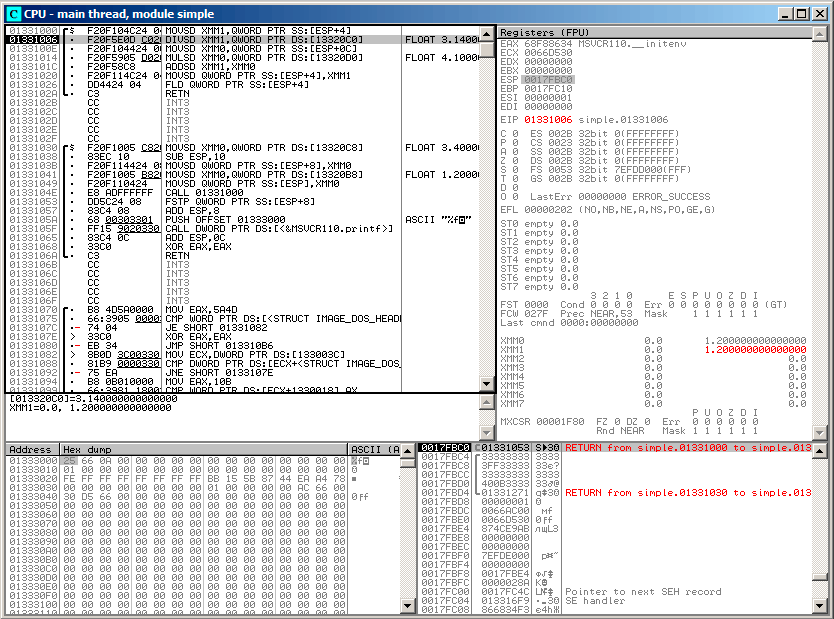
\includegraphics[scale=\FigScale]{patterns/205_floating_SIMD/simple_olly1.png}
\caption{\olly: \TT{MOVSD} \RU{загрузила значение}\EN{loads the value of} $a$ \RU{в}\EN{into} \XMM{1}}
\label{fig:FPU_SIMD_simple_olly1}
\end{figure}

\clearpage
\begin{figure}[H]
\centering
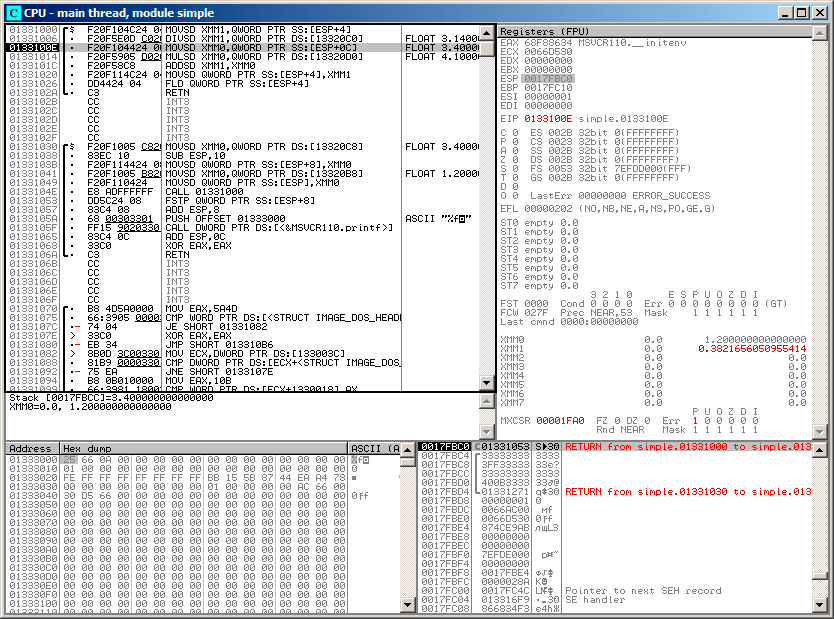
\includegraphics[scale=\FigScale]{patterns/205_floating_SIMD/simple_olly2.png}
\caption{\olly: \TT{DIVSD} \RU{вычислила}\EN{calculated} \gls{quotient} 
\RU{и оставила его в}\EN{and stored it in} \XMM{1}}
\label{fig:FPU_SIMD_simple_olly2}
\end{figure}

\clearpage
\begin{figure}[H]
\centering
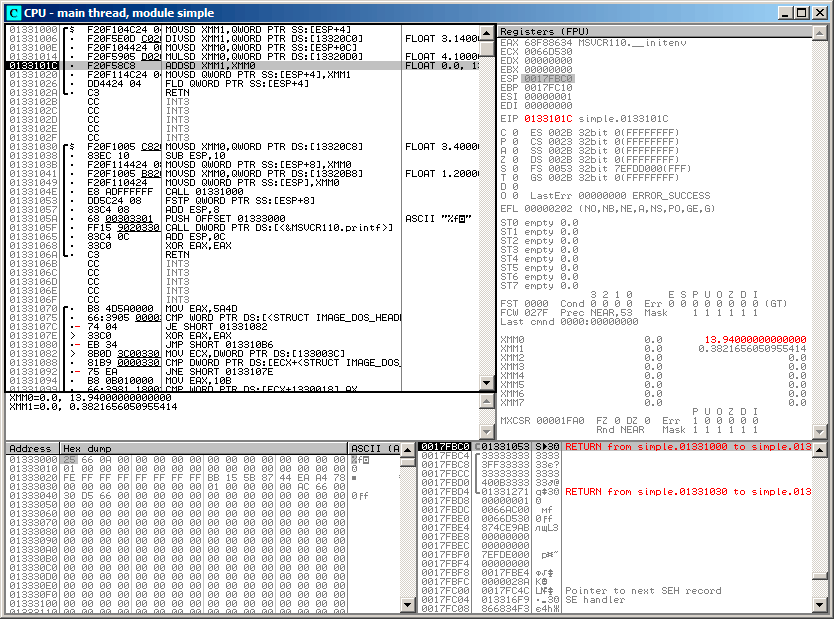
\includegraphics[scale=\FigScale]{patterns/205_floating_SIMD/simple_olly3.png}
\caption{\olly: \TT{MULSD} \RU{вычислила}\EN{calculated} \gls{product} \RU{и оставила его в}\EN{and stored it
in} \XMM{0}}
\label{fig:FPU_SIMD_simple_olly3}
\end{figure}

\clearpage
\begin{figure}[H]
\centering
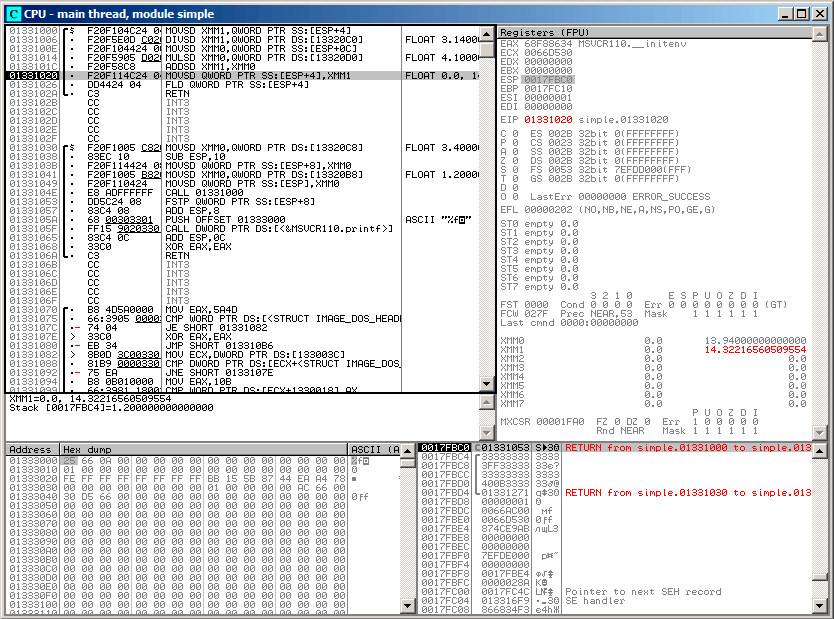
\includegraphics[scale=\FigScale]{patterns/205_floating_SIMD/simple_olly4.png}
\caption{\olly: \TT{ADDSD} \RU{прибавила значение в}\EN{adds value in} \XMM{0} \RU{к}\EN{to} \XMM{1}}
\label{fig:FPU_SIMD_simple_olly4}
\end{figure}

\clearpage
\begin{figure}[H]
\centering
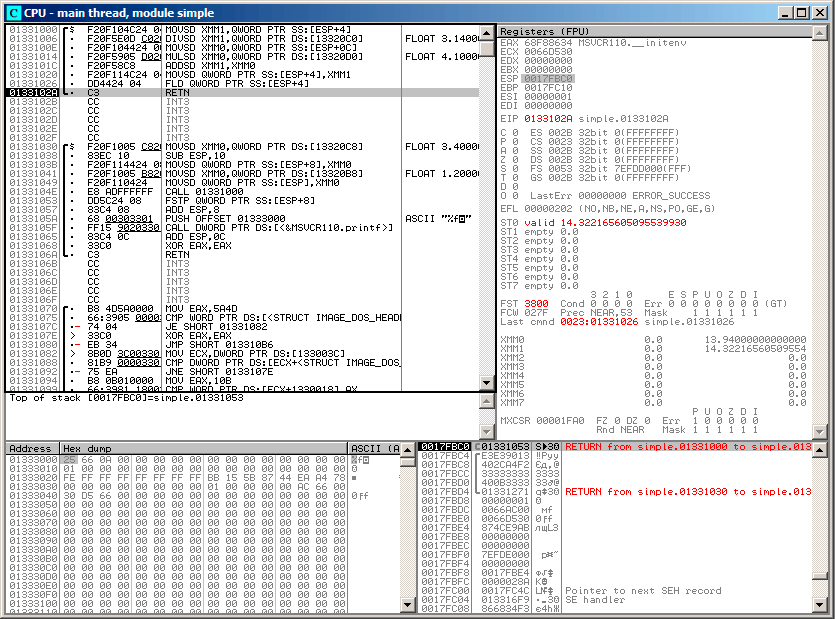
\includegraphics[scale=\FigScale]{patterns/205_floating_SIMD/simple_olly5.png}
\caption{\olly: \FLD \RU{оставляет результат ф-ции в}\EN{left function result in} \ST{0}}
\label{fig:FPU_SIMD_simple_olly5}
\end{figure}

\RU{Видно, что \olly показывает XMM-регистры как пары чисел в формате \Tdouble,
но используется только \IT{младшая} часть.}
\EN{We see that \olly shows the XMM registers as pairs of \Tdouble numbers,
but only the \IT{lower} part is used.}
\RU{Должно быть, \olly показывает их именно так, потому что сейчас исполняются SSE2-инструкции
с суффиксом \TT{-SD}.}
\EN{Apparently, \olly shows them in that format because the SSE2 instructions (suffixed with \TT{-SD}) 
are executed right now.}
\RU{Но конечно же, можно переключить отображение значений в регистрах и посмотреть содержимое
как 4 \Tfloat{}-числа или просто как 16 байт.}
\EN{But of course, it's possible to switch the register format and to see their contents as
4 \Tfloat{}-numbers or just as 16 bytes.}
\fi

\clearpage
\section{\RU{Передача чисел с плавающей запятой в аргументах}\EN{Passing floating point number via arguments}}

\lstinputlisting{patterns/12_FPU/2_passing_floats/pow.c}

\RU{Они передаются в младших половинах регистров}\EN{They are passed in the lower halves
of the} \XMM{0}-\XMM{3}\EN{ registers}.

\lstinputlisting[caption=\Optimizing MSVC 2012 x64]{patterns/205_floating_SIMD/pow_MSVC_2012_x64_Ox.asm}

\index{x86!\Instructions!MOVSD}
\index{x86!\Instructions!MOVSDX}
\RU{Инструкции}\EN{There is no} \TT{MOVSDX} \RU{нет в документации от}\EN{instruction in} 
Intel \cite{Intel} \AndENRU AMD \cite{AMD}\EN{ manuals}, 
\RU{там она называется просто}\EN{there it is called just} \TT{MOVSD}.
\RU{Таким образом, в процессорах x86 две инструкции с одинаковым именем}\EN{So there are two instructions
sharing the same name in x86} (\RU{о второй}\EN{about the other see}: \myref{REP_MOVSx}).
\RU{Возможно, в Microsoft решили избежать
путаницы и переименовали инструкцию в}\EN{Apparently, Microsoft developers wanted to get rid of the mess,
so they renamed it to} \TT{MOVSDX}.
\RU{Она просто загружает значение в младшую половину XMM-регистра}\EN{It just loads a value into
the lower half of a XMM register}.

\RU{Ф-ция }\TT{pow()} \RU{берет аргументы из}\EN{takes arguments from} \XMM{0} \AndENRU \XMM{1}, 
\RU{и возвращает результат в}\EN{and returns result in} \XMM{0}.
\RU{Далее он перекладывается в}\EN{It is then moved to} \RDX \ForENRU \printf. 
\RU{Почему}\EN{Why}? 
\RU{Честно говоря, не знаю, может быть, это потому что}\EN{Honestly speaking, I don't know, maybe because} 
\printf\EMDASH{}\RU{ф-ция с переменным количеством аргументов}\EN{is a variable arguments function}?

\lstinputlisting[caption=\Optimizing GCC 4.4.6 x64]{patterns/205_floating_SIMD/pow_GCC446_x64_O3.s.\LANG}

GCC \RU{работает понятнее}\EN{generates clearer output}. 
\RU{Значение для}\EN{The value for} \printf \RU{передается в}\EN{is passed in} \XMM{0}. 
\RU{Кстати, вот тот случай, когда в}\EN{By the way, here is a case when 1 is written into} \EAX
\ForENRU \printf \RU{записывается 1 --- это значит, что будет передан один аргумент в векторных регистрах, 
так того требует стандарт}\EN{---this means that one argument will be passed in vector registers,
just as the standard requires} \cite{SysVABI}.

\section{\RU{Пример с сравнением}\EN{Comparison example}}

\lstinputlisting{patterns/12_FPU/3_comparison/d_max.c}

\subsection{x64}

\lstinputlisting[caption=\Optimizing MSVC 2012 x64]{patterns/205_floating_SIMD/d_max_MSVC_2012_x64_Ox.asm}

\Optimizing MSVC \RU{генерирует очень понятный код}\EN{generates a code very easy to understand}.

\index{x86!\Instructions!COMISD}
\RU{Инструкция }\TT{COMISD} \RU{это}\EN{is} ``Compare Scalar Ordered Double-Precision Floating-Point 
Values and Set EFLAGS''. \RU{Собственно, это она и делает}\EN{Essentially, that is what it does}.\\
\\
\NonOptimizing MSVC \RU{генерирует более избыточно, но тоже всё понятно}\EN{generates more redundant code,
but it is still not hard to understand}:

\lstinputlisting[caption=MSVC 2012 x64]{patterns/205_floating_SIMD/d_max_MSVC_2012_x64.asm}

\index{x86!\Instructions!MAXSD}
\RU{А вот}\EN{However,} GCC 4.4.6 \RU{дошел в оптимизации дальше и применил инструкцию}
\EN{did more optimizations and used the} \TT{MAXSD} (``Return Maximum Scalar 
Double-Precision Floating-Point Value'')\RU{, которая просто выбирает максимальное значение}\EN{ instruction,
which just choose the maximum value}!

\lstinputlisting[caption=\Optimizing GCC 4.4.6 x64]{patterns/205_floating_SIMD/d_max_GCC446_x64_O3.s}

\clearpage
\subsection{x86}

\RU{Скомпилируем этот пример в MSVC 2012 с включенной оптимизацией:}
\EN{Let's compile this example in MSVC 2012 with optimization turned on:}

\lstinputlisting[caption=\Optimizing MSVC 2012 x86]{patterns/205_floating_SIMD/d_max_MSVC_2012_x86_Ox.asm}

\RU{Всё то же самое, только значения}\EN{Almost the same, but the values of} $a$ \AndENRU $b$ 
\RU{берутся из стека, а результат функции оставляется в}\EN{are taken from the stack and the function result 
is left in} \ST{0}.

\ifdefined\IncludeOlly
\RU{Если загрузить этот пример в}\EN{If we load this example in} \olly, 
\RU{увидим, как инструкция}\EN{we will see how the} \TT{COMISD} \RU{сравнивает значения и устанавливает/сбрасывает
флаги}\EN{instruction compares values and sets/clears the} \CF \AndENRU \PF\EN{ flags}:

\begin{figure}[H]
\centering
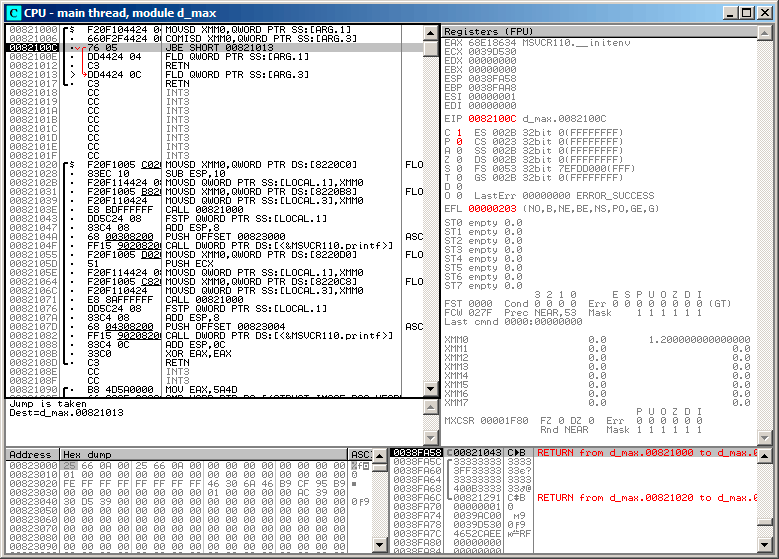
\includegraphics[scale=\FigScale]{patterns/205_floating_SIMD/d_max_olly.png}
\caption{\olly: \TT{COMISD} \RU{изменила флаги}\EN{changed} \CF \AndENRU \PF\EN{ flags}}
\label{fig:FPU_SIMD_d_max_olly}
\end{figure}
\fi

\section{\RU{Вычисление машинного эпсилона}\EN{Calculating machine epsilon}: x64 \AndENRU SIMD}
\label{machine_epsilon_x64_and_SIMD}

\RU{Вернемся к примеру ``вычисление машинного эпсилона'' для \Tdouble \lstref{machine_epsilon_double_c}.}
\EN{Let's revisit the ``calculating machine epsilon'' example for \Tdouble \lstref{machine_epsilon_double_c}.}

\RU{Теперь скомпилируем его для x64}\EN{Now we compile it for x64}:

\lstinputlisting[caption=\Optimizing MSVC 2012 x64]{patterns/205_floating_SIMD/epsilon_double_MSVC_2012_x64_Ox.asm}

\RU{Нет способа прибавить 1 к значению в 128-битном XMM-регистре, так что его нужно в начале поместить в память.}
\EN{There is no way to add 1 to a value in 128-bit XMM register, so it must be placed into memory.}

\RU{Впрочем, есть инструкция ADDSD (\IT{Add Scalar Double-Precision Floating-Point Values}),
которая может прибавить значение к младшей 64-битной части XMM-регистра игнорируя старшую половину,
но наверное MSVC 2012 пока недостаточно хорош для этого}
\EN{There is, however, the ADDSD instruction (\IT{Add Scalar Double-Precision Floating-Point Values}) 
which can add a value to the lowest 64-bit half of a XMM register while ignoring the higher one, 
but MSVC 2012 probably is not that good yet}
\footnote{\RU{В качестве упражнения, вы можете попробовать переработать этот код, чтобы избавиться 
от использования локального стека}\EN{As an exercise, you may try to rework this code to 
eliminate the usage of the local stack}.}.

\RU{Так или иначе, значение затем перезагружается в XMM-регистр и происходит вычитание.}
\EN{Nevertheless, the value is then reloaded to a XMM register and subtraction occurs.}
SUBSD \RU{это}\EN{is} ``Subtract Scalar Double-Precision Floating-Point Values'', 
\RU{т.е., операция производится над младшей 64-битной частью 128-битного XMM-регистра}
\EN{i.e., it operates on the lower 64-bit part of 128-bit XMM register}.
\RU{Результат возвращается в регистре XMM0}\EN{The result is returned in the XMM0 register}.

\input{patterns/205_floating_SIMD/FPU_PRNG/main}

\section{\RU{Итог}\EN{Summary}}

\RU{Во всех приведенных примерах, в XMM-регистрах используется только младшая половина регистра, там
хранится значение в формате IEEE 754}\EN{Only the lower half of XMM registers is used in all examples here, 
to store number in IEEE 754 format}.

\RU{Собственно, все инструкции с суффиксом}\EN{Essentially, all instructions prefixed by} 
\TT{-SD} (``Scalar Double-Precision'')\EMDASH{}\RU{это инструкции для работы с числами с плавающей 
запятой в формате IEEE 754, 
хранящиеся в младшей 64-битной половине XMM-регистра}\EN{are instructions working with floating point numbers
in IEEE 754 format, stored in the lower 64-bit half of a XMM register}.

\RU{Всё удобнее чем это было в FPU, видимо, сказывается тот факт, что расширения 
SIMD развивались не так хаотично как FPU в прошлом.}
\EN{And it is easier than in the FPU, probably because the SIMD extensions 
were evolved in a less chaotic way than the FPU ones in the past.}
\RU{Стековая модель регистров не используется}\EN{The stack register model is not used}.

\index{x86!\Instructions!ADDSS}
\index{x86!\Instructions!MOVSS}
\index{x86!\Instructions!COMISS}
% TODO: do this!
\RU{Если вы попробуете заменить в этих примерах}\EN{If you would try to replace} \Tdouble \RU{на}\EN{with} \Tfloat
\RU{, то инструкции будут использоваться те же,
только с суффиксом}\EN{in these examples, the same instructions will be used, but prefixed with} \TT{-SS} 
(``Scalar Single-Precision''), \RU{например}\EN{for example}, \TT{MOVSS}, \TT{COMISS}, \TT{ADDSS}, \RU{и т.д.}\EN{etc.}

``Scalar'' \RU{означает что SIMD-регистр будет хранить только одно значение, вместо нескольких}\EN{means that
the SIMD register will contain only one value instead of several}.
\RU{Инструкции, работающие с несколькими значениями в регистре одновременно, имеют ``Packed'' в названии}
\EN{Instructions working with several values in a register simultaneously have ``Packed'' in their name}.

\RU{Нужно также обратить внимание, что SSE2-инструкции работают с 64-битными числами (\Tdouble) в формате IEEE 754,
в то время как внутреннее представление в FPU --- 80-битные числа.}
\EN{Needless to say, the SSE2 instructions work with 64-bit IEEE 754 numbers (\Tdouble),
while the internal representation of the floating-point numbers in FPU is 80-bit numbers.}
\RU{Поэтому ошибок округления (\IT{round-off error}) в FPU может быть меньше чем в SSE2,
как следствие, можно сказать, работа с FPU может давать более точные результаты вычислений.}
\EN{Hence, the FPU may produce less round-off errors and as a consequence, FPU may give more precise
calculation results.}

\fi
\ifdefined\IncludeARM
\chapter{\EN{More about ARM}\RU{Еще немного об ARM}}

\section{\RU{Знак номера}\EN{Number sign} (\#) \RU{перед числом}\EN{before number}}

\RU{Компилятор Keil, \IDA и objdump предваряет все числа знаком номера (``\#''), например:}
\EN{The Keil compiler, \IDA and objdump precede all numbers with the ``\#'' number sign, for example:}
\lstref{Keil_number_sign}.
\RU{Но когда GCC 4.9 выдает результат на языке ассемблера, он так не делает, например:}
\EN{But when GCC 4.9 generates assembly language output, it doesn't, for example: }
\lstref{GCC_no_number_sign}.

\RU{Так что листинги для ARM в этой книге в каком-то смысле перемешаны.}
\EN{The ARM listings in this book are somewhat mixed.}

\RU{Я не знаю, как правильнее.}\EN{I'm not sure which method is right.}
\RU{Должно быть, всякий должен придерживаться тех правил, которые приняты в той среде,
в которой он работает.}
\EN{Supposedly, one should obey the rules accepted in environment he/she works in.}

% sections
\input{patterns/ARM/post_pre_index.tex}
\input{patterns/ARM/big_constants.tex}
\input{patterns/ARM/relocs.tex}

\fi
\ifdefined\IncludeMIPS
\chapter{\EN{MIPS-specific details}\RU{Кое-что специфичное для MIPS}}

% sections
\input{patterns/MIPS/big_constants.tex}

\section{\RU{Книги и прочие материалы о MIPS}\EN{Further reading about MIPS}}

\cite{MIPSRun}.

\fi

\part{\RU{Важные фундаментальные вещи}\EN{Important fundamentals}}

% chapters
\chapter{\SignedNumbersSectionName}
\label{sec:signednumbers}
\index{Signed numbers}

\newcommand{\URLS}{\href{http://go.yurichev.com/17117}{wikipedia}}

\RU{Методов представления чисел с знаком ``плюс'' или ``минус'' несколько\footnote{\URLS}, 
но в компьютерах обычно применяется метод ``дополнительный код'' или ``two's complement''.}
\EN{There are several methods for representing signed numbers\footnote{\URLS}, 
but ``two's complement'' is the most popular one in computers.}

\EN{Here is a table for some byte values:}
\RU{Вот таблица некоторые значений байтов:}

\begin{center}
\begin{tabular}{ | l | l | l | l | }
\hline
\cellcolor{blue!25} \RU{двоичное}\EN{binary} & 
\cellcolor{blue!25} \RU{шестнадцатеричное}\EN{hexadecimal} & 
\cellcolor{blue!25} \RU{беззнаковое}\EN{unsigned} &
\cellcolor{blue!25} \RU{знаковое}\EN{signed} (\RU{дополнительный код}\EN{2's complement}) \\
\hline
01111111 & 0x7f & 127 & 127 \\
\hline
01111110 & 0x7e & 126 & 126 \\
\hline
\multicolumn{4}{ |c| }{...} \\
\hline
00000110 & 0x6 & 6 & 6 \\
\hline
00000101 & 0x5 & 5 & 5 \\
\hline
00000100 & 0x4 & 4 & 4 \\
\hline
00000011 & 0x3 & 3 & 3 \\
\hline
00000010 & 0x2 & 2 & 2 \\
\hline
00000001 & 0x1 & 1 & 1 \\
\hline
00000000 & 0x0 & 0 & 0 \\
\hline
11111111 & 0xff & 255 & -1 \\
\hline
11111110 & 0xfe & 254 & -2 \\
\hline
11111101 & 0xfd & 253 & -3 \\
\hline
11111100 & 0xfc & 252 & -4 \\
\hline
11111011 & 0xfb & 251 & -5 \\
\hline
11111010 & 0xfa & 250 & -6 \\
\hline
\multicolumn{4}{ |c| }{...} \\
\hline
10000010 & 0x82 & 130 & -126 \\
\hline
10000001 & 0x81 & 129 & -127 \\
\hline
10000000 & 0x80 & 128 & -128 \\
\hline
\end{tabular}
\end{center}

\index{x86!\Instructions!JA}
\index{x86!\Instructions!JB}
\index{x86!\Instructions!JL}
\index{x86!\Instructions!JG}
\RU{Разница в подходе к знаковым/беззнаковым числам, собственно, нужна потому что, например, 
если представить \TT{0xFFFFFFFE} и \TT{0x0000002} как беззнаковое, то первое число ($4294967294$) больше второго ($2$). 
Если их оба представить как знаковые, то первое будет $-2$, которое, разумеется, меньше чем второе ($2$).
Вот почему инструкции для условных переходов~(\myref{sec:Jcc}) представлены в обоих версиях ~--- 
и для знаковых сравнений (например, \JG, \JL) и для беззнаковых (\JA, \JB).}
\EN{The difference between signed and unsigned numbers is that if we represent \TT{0xFFFFFFFE} and \TT{0x0000002} 
as unsigned, then the first number ($4294967294$) is bigger than the second one($2$). 
If we represent them both as signed, the first one is to be $-2$, and it is smaller than the second ($2$). 
That is the reason why conditional jumps~(\myref{sec:Jcc}) are present both for signed (e.g. \JG, \JL) 
and unsigned (\JA, \JB) operations.} \\
\\
\RU{Для простоты, вот что нужно знать}\EN{For the sake of simplicity, that is what one need to know}:
\begin{itemize}
\item \RU{Числа бывают знаковые и беззнаковые}\EN{Number can be signed or unsigned}.

\item \RU{Знаковые типы в \CCpp}\EN{\CCpp signed types}:
  \begin{itemize}
    \item \TT{int64\_t} (-9223372036854775806..9223372036854775807) \OrENRU \\
                \TT{0x8000000000000000..0x7FFFFFFFFFFFFFFF}),
    \item \Tint (-2147483646..2147483647 \OrENRU \TT{0x80000000..0x7FFFFFFF}),
    \item \Tchar (-127..128 \OrENRU \TT{0x7F..0x80}),
    \item \TT{ssize\_t}.
   \end{itemize}

	\RU{Беззнаковые}\EN{Unsigned}: 
  \begin{itemize}
   \item \TT{uint64\_t} (0..18446744073709551615 \OrENRU \TT{0..0xFFFFFFFFFFFFFFFF}),
   \item \TT{unsigned int} (0..4294967295 \OrENRU \TT{0..0xFFFFFFFF}),
   \item \TT{unsigned char} (0..255 \OrENRU \TT{0..0xFF}), 
   \item \TT{size\_t}.
  \end{itemize}

\item \RU{У знаковых чисел знак определяется самым старшим битом: 1 означает ``минус'', 0 означает ``плюс''}
	\EN{Signed types have the sign in the most significant bit: 1 mean ``minus'', 0 mean ``plus''}.

\item \EN{Promoting to a larger data types is simple:}
      \RU{Преобразование в б\'{о}льшие типы данных обходится легко:} \myref{subsec:sign_extending_32_to_64}.

\item \EN{Negation is simple: just invert all bits and add 1.}
\RU{Изменить знак легко: просто инвертируйте все биты и прибавьте 1.}
\EN{We can remember that a number of inverse sign is located 
on the opposite side at the same proximity from zero.}
\RU{Мы можем заметить, что число другого знака находится на другой стороне на том же расстоянии от нуля.}
\RU{Прибавление единицы необходимо из-за присутствия нуля посредине.}
\EN{The addition of one is needed because zero is present in the middle.}

\index{x86!\Instructions!IDIV}
\index{x86!\Instructions!DIV}
\index{x86!\Instructions!IMUL}
\index{x86!\Instructions!MUL}
\index{x86!\Instructions!CBW}
\index{x86!\Instructions!CWD}
\index{x86!\Instructions!CWDE}
\index{x86!\Instructions!CDQ}
\index{x86!\Instructions!CDQE}
\index{x86!\Instructions!MOVSX}
\index{x86!\Instructions!SAR}
\item \RU{Инструкции сложения и вычитания работают одинаково хорошо и для знаковых и для беззнаковых значений}
	\EN{The addition and subtraction operations work well for both signed and unsigned values}.
	\RU{Но для операций умножения и деления, в x86 имеются разные инструкции}
	\EN{But for multiplication and division operations, x86 has different instructions}:
	\TT{IDIV}/\TT{IMUL} \RU{для знаковых}\EN{for signed}
	\AndENRU \TT{DIV}/\TT{MUL} \RU{для беззнаковых}\EN{for unsigned}.
\ifx\LITE\undefined
\item \RU{Еще инструкции работающие с знаковыми числами}\EN{Here are some more instructions that work with signed numbers}:
	\TT{CBW/CWD/CWDE/CDQ/CDQE} (\myref{ins:CBW_CWD_etc}), \TT{MOVSX} (\myref{MOVSX}), \TT{SAR} (\myref{ins:SAR}).
\fi
\end{itemize}

\iffalse
% FIXME rework!
\section{\RU{Переполнение integer}\EN{Integer overflow}}

\RU{Бывает так, что ошибки представления знаковых/беззнаковых могут привести к уязвимости 
\IT{переполнение integer}.}
\EN{It is worth noting that the incorrect representation of a number can lead to integer overflow vulnerabilities.}

\RU{Например, есть некий сервис, который принимает по сети некие пакеты. 
В пакете есть заголовок где указана длина пакета. Это 32-битное значение. 
В процессе приема пакета, 
сервис проверяет это значение и сверяет, больше ли оно чем максимальный размер пакета, скажем, константа
\TT{MAX\_PACKET\_SIZE} (например, 10 килобайт), и если да, то пакет отвергается как некорректный. 
Сравнение знаковое. Злоумышленник подставляет значение \TT{0xFFFFFFFF}. Это число трактуется как знаковое $-1$ 
и оно меньше чем $10000$. Проверка проходит. Продолжаем дальше и копируем этот пакет куда-нибудь себе 
в сегмент данных\dots вызов функции \TT{memcpy (dst, src, 0xFFFFFFFF)} скорее всего, 
затрет много чего внутри процесса.}
\EN{For example, we have a network service and it receives network packets. 
In the packets there is a field where the subpacket length is encoded. 
It is a 32-bit value. 
After the receiving of the network packet, the service checks the field and if it is larger than 
some \TT{MAX\_PACKET\_SIZE} (let's say, 10 kilobytes), the packet is rejected as incorrect.
The comparison is signed. The intruder set this value to \TT{0xFFFFFFFF}.
While comparing, this number is considered as signed $-1$ and it is less than 10 kilobytes. 
No error here. 
The service would then like to copy the subpacket to another place in memory and calls the 
\TT{memcpy (dst, src, 0xFFFFFFFF)} function: this operation, rapidly garbles a lot of 
of process memory.}

\RU{Немного подробнее}\EN{More about it}: \cite{Phrack3C0A}.
% TODO example!
\fi

\chapter{Endianness\RU{ (порядок байт)}}
\label{sec:endianness}

\RU{Endianness (порядок байт) это способ представления чисел в памяти}
\EN{The endianness is a way of representing values in memory}.

\section{Big-endian\RU{ (от старшего к младшему)}}

\RU{Число}\EN{The} \TT{0x12345678} \RU{будет представлено в памяти так}\EN{value will be represented in memory as}:

\begin{center}
\begin{tabular}{ | l | l | }
\hline
\cellcolor{blue!25} \RU{адрес в памяти}\EN{address in memory} & \cellcolor{blue!25} \RU{значение байта}\EN{byte value} \\
\hline
+0 & 0x12 \\
\hline
+1 & 0x34 \\
\hline
+2 & 0x56 \\
\hline
+3 & 0x78 \\
\hline
\end{tabular}
\end{center}

\RU{CPU с таким порядком включают в себя}\EN{Big-endian CPUs include} Motorola 68k, IBM POWER.

\section{Little-endian\RU{ (от младшего к старшему)}}

\RU{Число}\EN{AThe \TT{0x12345678} \RU{будет представлено в памяти так}\EN{value will be represented in memory as}:

\begin{center}
\begin{tabular}{ | l | l | }
\hline
\cellcolor{blue!25} \RU{адрес в памяти}\EN{address in memory} & \cellcolor{blue!25} \RU{значение байта}\EN{byte value} \\
\hline
+0 & 0x78 \\
\hline
+1 & 0x56 \\
\hline
+2 & 0x34 \\
\hline
+3 & 0x12 \\
\hline
\end{tabular}
\end{center}

\RU{CPU с таким порядком байт включают в себя}\EN{Little-endian CPUs include} Intel x86.

\section{\Example}

\RU{У меня есть big-endian Linux для MIPS заинсталированный в QEMU}
\EN{I have big-endian MIPS Linux installed and ready in QEMU}
\footnote{\RU{Я скачал его здесь}\EN{I've uploaded it here}: \url{http://go.yurichev.com/17008}}.

\RU{И вот я сделал простой пример}\EN{And I have compiled this simple example}:

\begin{lstlisting}
#include <stdio.h>

int main()
{
	int v, i;

	v=123;

	printf ("%02X %02X %02X %02X\n", 
		*(char*)&v,
		*(((char*)&v)+1),
		*(((char*)&v)+2),
		*(((char*)&v)+3));
};
\end{lstlisting}

\RU{И запустил его}\EN{And after running it I get}:

\begin{lstlisting}
root@debian-mips:~# ./a.out 
00 00 00 7B
\end{lstlisting}

\RU{Это оно и есть}\EN{That is it}.
0x7B \RU{это}\EN{is} 123 \RU{в десятичном виде}\EN{in decimal}.
\RU{В little-endian-архитектуре, 7B будет первым байтом (вы можете это проверить в x86 или x86-64),
но здесь он последний, потому что старший байт идет первым.}
\EN{In little-endian architectures, 7B will be the first byte (you can check on x86 or x86-64), 
but here it is the last one, because the highest byte goes first.}

\RU{Вот почему имеются разные дистрибутивы Linux для MIPS}
\EN{That's why there are separate Linux distributions for MIPS} 
(``mips'' (big-endian) \AndENRU ``mipsel'' (little-endian)).
\RU{Программа скомпилированная для одного соглашения об endiannes, не сможет работать в OS использующей
другое соглашение.}
\EN{It is impossible for a binary compiled for one endianness to work on an OS with different endianness.}\\
\\
\RU{Еще один пример связанный с big-endian в MIPS в этой книге:}
\EN{There is another example of MIPS big-endiannes in this book:} \ref{MIPS_structure_big_endian}.

\section{Bi-endian\RU{ (переключаемый порядок)}}

\RU{CPU поддерживающие оба порядка, и его можно переключать, включают в себя}
\EN{CPUs that may switch between endianness are} ARM, PowerPC, SPARC, MIPS, \ac{IA64}, \RU{и т.д.}\EN{etc.}

\section{\RU{Конвертирование}\EN{Converting data}}

\index{TCP/IP}
\RU{Сетевые пакеты TCP/IP используют соглашение big-endian, вот почему программа, работающая на little-endian архитектуре
должна конвертировать значения используя ф-ции}
\EN{TCP/IP network data packets use the big-endian conventions, so that is why a program working on a little-endian architecture
should convert the values using the} \TT{htonl()} \AndENRU \TT{htons()}\EN{ functions}.

\RU{Порядок байт big-endian в среде TCP/IP также называется}
\EN{In TCP/IP, big-endian is also called} ``network byte order'',
\RU{а}\EN{while} little-endian\EMDASH{}``host byte order''.

\index{x86!\Instructions!BSWAP}
\RU{Инструкция }{The }\TT{BSWAP} \RU{также может использоваться для конвертирования}
\EN{instruction can also be used for conversion}.


\chapter{\RU{Память}\EN{Memory}}

\RU{Есть три основных типа памяти:}
\EN{There are 3 main types of memory:}

\begin{itemize}
\item \RU{Глобальная память}\EN{Global memory}.
\ac{AKA} ``static memory allocation''.
\RU{Нет нужды явно выделять, выделение происходит просто при объявлении переменных/массивов 
глобально.}
\EN{No need to allocate explicitly, allocation is done just by declaring variables/arrays 
globally.}
\RU{Это глобальные переменные расположенные в сегменте данных или констант.}
\EN{This is global variables residing in data or constant segments.}
\RU{Доступны глобально (поэтому считаются \glslink{anti-pattern}{анти-паттерном}).}
\EN{Available globally (hence, considered as \gls{anti-pattern}).}
\RU{Не удобны для буферов/массивов, потому что должны иметь фиксированный размер.}
\EN{Not convenient for buffers/arrays, because must have fixed size.}
\RU{Переполнения буфера случающиеся здесь, обычно перезаписывают переменные или буферы
расположеные рядом в памяти.}
\EN{Buffer overflows occuring here usually overwriting variable or buffer residing next in memory.}
\RU{Пример в этой книге}\EN{Example in this book}: \ref{scanf_global_variable}.

\item \RU{Стек}\EN{Stack}.
\ac{AKA} ``allocate on stack''.
\RU{Выделение происходит просто при объявлении переменных/массивов локально в ф-ции.}
\EN{Allocation is done just by declaring variables/arrays locally in the function.}
\RU{Обычно это локальные для ф-ции переменные}\EN{This is usually local to function variables}.
\RU{Иногда эти локальные переменные также доступны и для нисходящих ф-ций (если ф-ция передает
указатель на переменную в следующую ф-цию).}
\EN{Sometimes these local variable are also available to descending functions (if one passing
pointer to variable to the function to be executed).}
\RU{Выделение и освобождение очень быстрое, достаточно просто сдвига \ac{SP}.}
\EN{Allocation and deallocation are very fast, \ac{SP} only needs to be shifted.}
\index{\CStandardLibrary!alloca()}
\EN{But also not convenient for buffers/arrays, because buffer size should be fixed at some length,
unless \TT{alloca()} (\ref{alloca}) (or variable-length array) is used.}
\RU{Но так же не удобно для буферов/массивов, потому что размер буфера фиксирован,
если только не используется \TT{alloca()} (\ref{alloca}) (или массив с переменной длиной).}
\RU{Переполнение буфера обычно перезаписывает важные структуры стека}\EN{Buffer overflow usually 
overwrites important stack structures}: \ref{subsec:bufferoverflow}.

\index{\CStandardLibrary!malloc()}
\index{\CStandardLibrary!free()}
\item \RU{Куча (\IT{heap}}\EN{Heap}. 
\ac{AKA} ``dynamic memory allocation''.
\RU{Выделение происходит при помощи вызова}\EN{Allocation is done by calling} 
\TT{malloc()/free()} \OrENRU \TT{new/delete} \InENRU \Cpp.
\RU{Самый удобный метод: размер блока может быть задан во время исполнения}\EN{Most convenient 
method: block size may be set in runtime}.
\index{\CStandardLibrary!realloc()}
\RU{Изменение размера возможно (при помощи \TT{realloc()}), но может быть медленным.}
\EN{Resizing is possible  (using \TT{realloc()}), but may be slow.}
\RU{Это самый медленный метод выделения памяти: аллокатор памяти должен поддерживать и обновлять
все управляющие структуры во время выделения и освобождения.}
\EN{This is slowest way to allocate memory: 
memory allocator must support and update all control structures while
allocating and deallocating.}
\RU{Переполнение буфера обычно перезаписывает все эти структуры}\EN{Buffer overflows are usually 
overwrites these structures}.
\RU{Выделения в куче также ведут к проблеме утечек памяти: каждый выделенный блок должен быть
явно освобожден, но кто-то может забыть об этом, или делать это неправильно.}
\EN{Heap allocations is also source of memory leak problem: each memory block should be deallocated
explicitly, but one may forgot about it, or do it incorrectly.}
\index{\CStandardLibrary!free()}
\RU{Еще одна проблема это ``использовать после освобождения'' --- использовать блок памяти после
того как \TT{free()} был вызван на нем, это тоже очень опасно.}
\EN{Another problem is ``use after free''---using a memory block after \TT{free()} was called on it,
which is very dangerous.}
\RU{Пример в этой книге}\EN{Example in this book}: \ref{struct_malloc_example}.

\end{itemize}


\ifx\LITE\undefined
\partold{\EN{Slightly more advanced examples}\RU{Более сложные примеры}}

\newcommand{\CURPATH}{advanced/030_dbl_neg}
\EN{\section{Text strings}

\subsection{\CCpp}

\label{C_strings}
The normal C strings are zero-terminated (\ac{ASCIIZ}-strings).

The reason why the C string format is as it is (zero-terminated) is apparently historical.
In [Dennis M. Ritchie, \IT{The Evolution of the Unix Time-sharing System}, (1979)]
we read:

\begin{framed}
\begin{quotation}
A minor difference was that the unit of I/O was the word, not the byte, because the PDP-7 was a word-addressed
machine. In practice this meant merely that all programs dealing with character streams ignored null
characters, because null was used to pad a file to an even number of characters.
\end{quotation}
\end{framed}

\myindex{Hiew}

In Hiew or FAR Manager these strings looks like this:

\begin{lstlisting}
int main()
{
	printf ("Hello, world!\n");
};
\end{lstlisting}

\begin{figure}[H]
\centering
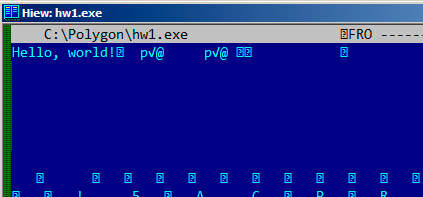
\includegraphics[scale=\NormalScale]{digging_into_code/strings/C-string.png}
\caption{Hiew}
\end{figure}

% FIXME видно \n в конце, потом пробел

\subsection{Borland Delphi}
\myindex{Pascal}
\myindex{Borland Delphi}

The string in Pascal and Borland Delphi is preceded by an 8-bit or 32-bit string length.

For example:

\begin{lstlisting}[caption=Delphi]
CODE:00518AC8                 dd 19h
CODE:00518ACC aLoading___Plea db 'Loading... , please wait.',0

...

CODE:00518AFC                 dd 10h
CODE:00518B00 aPreparingRun__ db 'Preparing run...',0
\end{lstlisting}

\subsection{Unicode}

\myindex{Unicode}

Often, what is called Unicode is a methods for encoding strings where each character occupies 2 bytes or 16 bits.
This is a common terminological mistake.
Unicode is a standard for assigning a number to each character in the many writing systems of the 
world, but does not describe the encoding method.

\myindex{UTF-8}
\myindex{UTF-16LE}
The most popular encoding methods are: UTF-8 (is widespread in Internet and *NIX systems) and UTF-16LE (is used in Windows).

\subsubsection{UTF-8}

\myindex{UTF-8}
UTF-8 is one of the most successful methods for
encoding characters.
All Latin symbols are encoded just like in ASCII,
and the symbols beyond the ASCII table are encoded using several bytes.
0 is encoded as
before, so all standard C string functions work with UTF-8 strings just like any other string.

Let's see how the symbols in various languages are encoded in UTF-8 and how it looks like in FAR, using the 437 codepage
\footnote{The example and translations was taken from here: 
\url{http://go.yurichev.com/17304}}:

\begin{figure}[H]
\centering
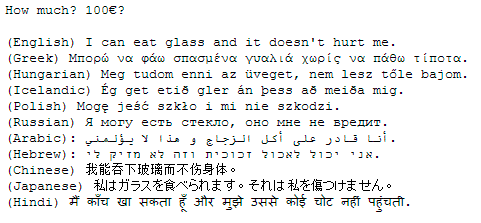
\includegraphics[scale=\NormalScale]{digging_into_code/strings/multilang_sampler.png}
\end{figure}

% FIXME: cut it
\begin{figure}[H]
\centering
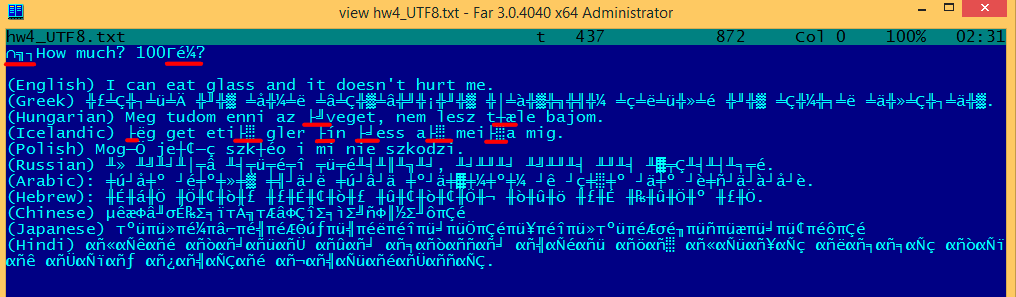
\includegraphics[scale=\FigScale]{digging_into_code/strings/multilang_sampler_UTF8.png}
\caption{FAR: UTF-8}
\end{figure}

As you can see, the English language string looks the same as it is in ASCII.

The Hungarian language uses some Latin symbols plus symbols with diacritic marks.

These symbols are encoded using several bytes, these are underscored with red.
It's the same story with the Icelandic and Polish languages.

There is also the \q{Euro} currency symbol at the start, which is encoded with 3 bytes.

The rest of the writing systems here have no connection with Latin.

At least in Russian, Arabic, Hebrew and Hindi we can see some recurring bytes, and that is not surprise:
all symbols from a writing system are usually located in the same Unicode table, so their code begins with
the same numbers.

At the beginning, before the \q{How much?} string we see 3 bytes, which are in fact the \ac{BOM}.
The \ac{BOM} defines the encoding system to be
used.

\subsubsection{UTF-16LE}

\myindex{UTF-16LE}
\myindex{Windows!Win32}
Many win32 functions in Windows have the suffixes \TT{-A} and \TT{-W}.
The first type of functions works
with normal strings, the other with UTF-16LE strings (\IT{wide}).

In the second case, each symbol is usually stored in a 16-bit value of type \IT{short}.

The Latin symbols in UTF-16 strings look in Hiew or FAR like they are interleaved with zero byte:

\begin{lstlisting}
int wmain()
{
	wprintf (L"Hello, world!\n");
};
\end{lstlisting}

\begin{figure}[H]
\centering
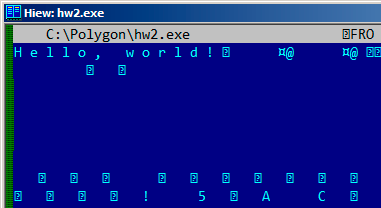
\includegraphics[scale=\NormalScale]{digging_into_code/strings/UTF16-string.png}
\caption{Hiew}
\end{figure}

We can see this often in \gls{Windows NT} system files:

\begin{figure}[H]
\centering
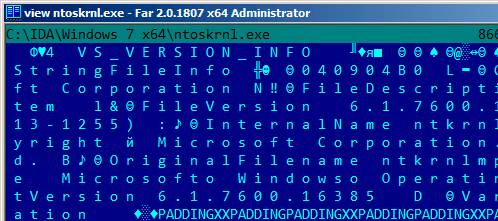
\includegraphics[scale=\NormalScale]{digging_into_code/strings/ntoskrnl_UTF16.png}
\caption{Hiew}
\end{figure}

\myindex{IDA}
Strings with characters that occupy exactly 2 bytes are called \q{Unicode} in \IDA:

\begin{lstlisting}
.data:0040E000 aHelloWorld:
.data:0040E000                 unicode 0, <Hello, world!>
.data:0040E000                 dw 0Ah, 0
\end{lstlisting}

Here is how the Russian language string is encoded in UTF-16LE:

\begin{figure}[H]
\centering
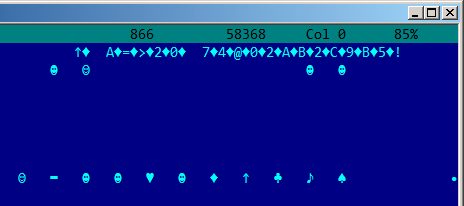
\includegraphics[scale=\NormalScale]{digging_into_code/strings/russian_UTF16.png}
\caption{Hiew: UTF-16LE}
\end{figure}

What we can easily spot is that the symbols are interleaved by the diamond character (which has the ASCII code of 4).
Indeed, the Cyrillic symbols are located in the fourth Unicode plane
\footnote{\href{http://go.yurichev.com/17003}{wikipedia}}.
Hence, all Cyrillic symbols in UTF-16LE are located in the \TT{0x400-0x4FF} range.

Let's go back to the example with the string written in multiple languages.
Here is how it looks like in UTF-16LE.

% FIXME: cut it
\begin{figure}[H]
\centering
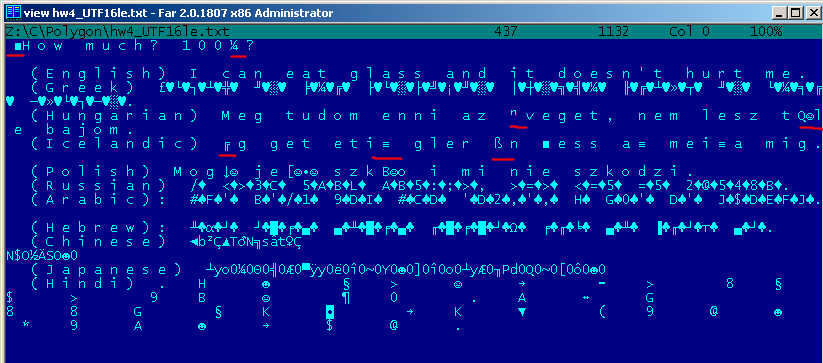
\includegraphics[scale=\FigScale]{digging_into_code/strings/multilang_sampler_UTF16.png}
\caption{FAR: UTF-16LE}
\end{figure}

Here we can also see the \ac{BOM} in the beginning.
All Latin characters are interleaved with a zero byte.

Some characters with diacritic marks (Hungarian and Icelandic languages) are also underscored in red.

% TODO: strings *NIX utility. procmonitor also shows strings...

% subsection:
\input{digging_into_code/strings/base64_EN}

}

\renewcommand{\CURPATH}{advanced/050_strstr}
\EN{\section{Text strings}

\subsection{\CCpp}

\label{C_strings}
The normal C strings are zero-terminated (\ac{ASCIIZ}-strings).

The reason why the C string format is as it is (zero-terminated) is apparently historical.
In [Dennis M. Ritchie, \IT{The Evolution of the Unix Time-sharing System}, (1979)]
we read:

\begin{framed}
\begin{quotation}
A minor difference was that the unit of I/O was the word, not the byte, because the PDP-7 was a word-addressed
machine. In practice this meant merely that all programs dealing with character streams ignored null
characters, because null was used to pad a file to an even number of characters.
\end{quotation}
\end{framed}

\myindex{Hiew}

In Hiew or FAR Manager these strings looks like this:

\begin{lstlisting}
int main()
{
	printf ("Hello, world!\n");
};
\end{lstlisting}

\begin{figure}[H]
\centering
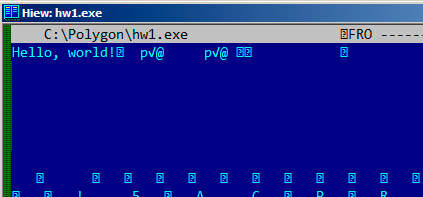
\includegraphics[scale=\NormalScale]{digging_into_code/strings/C-string.png}
\caption{Hiew}
\end{figure}

% FIXME видно \n в конце, потом пробел

\subsection{Borland Delphi}
\myindex{Pascal}
\myindex{Borland Delphi}

The string in Pascal and Borland Delphi is preceded by an 8-bit or 32-bit string length.

For example:

\begin{lstlisting}[caption=Delphi]
CODE:00518AC8                 dd 19h
CODE:00518ACC aLoading___Plea db 'Loading... , please wait.',0

...

CODE:00518AFC                 dd 10h
CODE:00518B00 aPreparingRun__ db 'Preparing run...',0
\end{lstlisting}

\subsection{Unicode}

\myindex{Unicode}

Often, what is called Unicode is a methods for encoding strings where each character occupies 2 bytes or 16 bits.
This is a common terminological mistake.
Unicode is a standard for assigning a number to each character in the many writing systems of the 
world, but does not describe the encoding method.

\myindex{UTF-8}
\myindex{UTF-16LE}
The most popular encoding methods are: UTF-8 (is widespread in Internet and *NIX systems) and UTF-16LE (is used in Windows).

\subsubsection{UTF-8}

\myindex{UTF-8}
UTF-8 is one of the most successful methods for
encoding characters.
All Latin symbols are encoded just like in ASCII,
and the symbols beyond the ASCII table are encoded using several bytes.
0 is encoded as
before, so all standard C string functions work with UTF-8 strings just like any other string.

Let's see how the symbols in various languages are encoded in UTF-8 and how it looks like in FAR, using the 437 codepage
\footnote{The example and translations was taken from here: 
\url{http://go.yurichev.com/17304}}:

\begin{figure}[H]
\centering
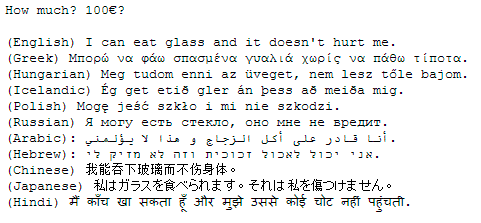
\includegraphics[scale=\NormalScale]{digging_into_code/strings/multilang_sampler.png}
\end{figure}

% FIXME: cut it
\begin{figure}[H]
\centering
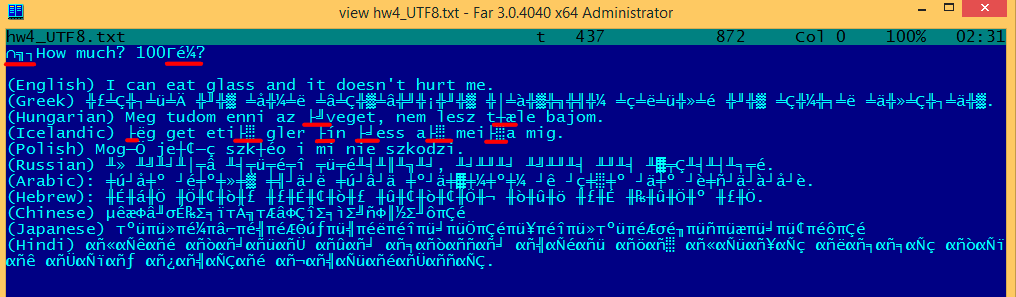
\includegraphics[scale=\FigScale]{digging_into_code/strings/multilang_sampler_UTF8.png}
\caption{FAR: UTF-8}
\end{figure}

As you can see, the English language string looks the same as it is in ASCII.

The Hungarian language uses some Latin symbols plus symbols with diacritic marks.

These symbols are encoded using several bytes, these are underscored with red.
It's the same story with the Icelandic and Polish languages.

There is also the \q{Euro} currency symbol at the start, which is encoded with 3 bytes.

The rest of the writing systems here have no connection with Latin.

At least in Russian, Arabic, Hebrew and Hindi we can see some recurring bytes, and that is not surprise:
all symbols from a writing system are usually located in the same Unicode table, so their code begins with
the same numbers.

At the beginning, before the \q{How much?} string we see 3 bytes, which are in fact the \ac{BOM}.
The \ac{BOM} defines the encoding system to be
used.

\subsubsection{UTF-16LE}

\myindex{UTF-16LE}
\myindex{Windows!Win32}
Many win32 functions in Windows have the suffixes \TT{-A} and \TT{-W}.
The first type of functions works
with normal strings, the other with UTF-16LE strings (\IT{wide}).

In the second case, each symbol is usually stored in a 16-bit value of type \IT{short}.

The Latin symbols in UTF-16 strings look in Hiew or FAR like they are interleaved with zero byte:

\begin{lstlisting}
int wmain()
{
	wprintf (L"Hello, world!\n");
};
\end{lstlisting}

\begin{figure}[H]
\centering
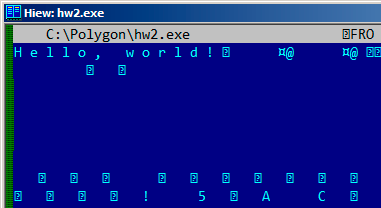
\includegraphics[scale=\NormalScale]{digging_into_code/strings/UTF16-string.png}
\caption{Hiew}
\end{figure}

We can see this often in \gls{Windows NT} system files:

\begin{figure}[H]
\centering
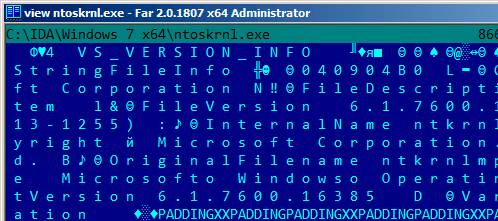
\includegraphics[scale=\NormalScale]{digging_into_code/strings/ntoskrnl_UTF16.png}
\caption{Hiew}
\end{figure}

\myindex{IDA}
Strings with characters that occupy exactly 2 bytes are called \q{Unicode} in \IDA:

\begin{lstlisting}
.data:0040E000 aHelloWorld:
.data:0040E000                 unicode 0, <Hello, world!>
.data:0040E000                 dw 0Ah, 0
\end{lstlisting}

Here is how the Russian language string is encoded in UTF-16LE:

\begin{figure}[H]
\centering
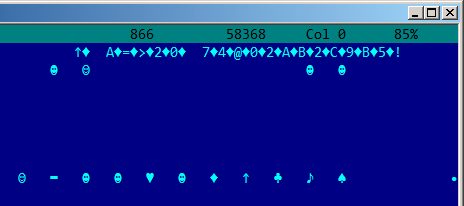
\includegraphics[scale=\NormalScale]{digging_into_code/strings/russian_UTF16.png}
\caption{Hiew: UTF-16LE}
\end{figure}

What we can easily spot is that the symbols are interleaved by the diamond character (which has the ASCII code of 4).
Indeed, the Cyrillic symbols are located in the fourth Unicode plane
\footnote{\href{http://go.yurichev.com/17003}{wikipedia}}.
Hence, all Cyrillic symbols in UTF-16LE are located in the \TT{0x400-0x4FF} range.

Let's go back to the example with the string written in multiple languages.
Here is how it looks like in UTF-16LE.

% FIXME: cut it
\begin{figure}[H]
\centering
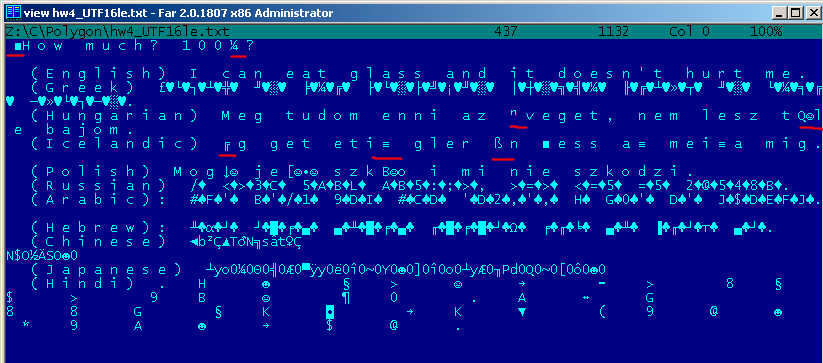
\includegraphics[scale=\FigScale]{digging_into_code/strings/multilang_sampler_UTF16.png}
\caption{FAR: UTF-16LE}
\end{figure}

Here we can also see the \ac{BOM} in the beginning.
All Latin characters are interleaved with a zero byte.

Some characters with diacritic marks (Hungarian and Icelandic languages) are also underscored in red.

% TODO: strings *NIX utility. procmonitor also shows strings...

% subsection:
\input{digging_into_code/strings/base64_EN}

}

\renewcommand{\CURPATH}{advanced/100_fahrenheit}
\EN{\section{Text strings}

\subsection{\CCpp}

\label{C_strings}
The normal C strings are zero-terminated (\ac{ASCIIZ}-strings).

The reason why the C string format is as it is (zero-terminated) is apparently historical.
In [Dennis M. Ritchie, \IT{The Evolution of the Unix Time-sharing System}, (1979)]
we read:

\begin{framed}
\begin{quotation}
A minor difference was that the unit of I/O was the word, not the byte, because the PDP-7 was a word-addressed
machine. In practice this meant merely that all programs dealing with character streams ignored null
characters, because null was used to pad a file to an even number of characters.
\end{quotation}
\end{framed}

\myindex{Hiew}

In Hiew or FAR Manager these strings looks like this:

\begin{lstlisting}
int main()
{
	printf ("Hello, world!\n");
};
\end{lstlisting}

\begin{figure}[H]
\centering
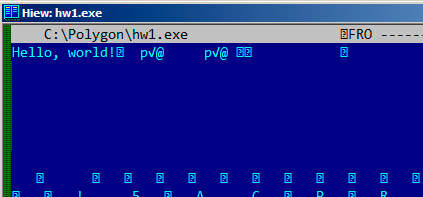
\includegraphics[scale=\NormalScale]{digging_into_code/strings/C-string.png}
\caption{Hiew}
\end{figure}

% FIXME видно \n в конце, потом пробел

\subsection{Borland Delphi}
\myindex{Pascal}
\myindex{Borland Delphi}

The string in Pascal and Borland Delphi is preceded by an 8-bit or 32-bit string length.

For example:

\begin{lstlisting}[caption=Delphi]
CODE:00518AC8                 dd 19h
CODE:00518ACC aLoading___Plea db 'Loading... , please wait.',0

...

CODE:00518AFC                 dd 10h
CODE:00518B00 aPreparingRun__ db 'Preparing run...',0
\end{lstlisting}

\subsection{Unicode}

\myindex{Unicode}

Often, what is called Unicode is a methods for encoding strings where each character occupies 2 bytes or 16 bits.
This is a common terminological mistake.
Unicode is a standard for assigning a number to each character in the many writing systems of the 
world, but does not describe the encoding method.

\myindex{UTF-8}
\myindex{UTF-16LE}
The most popular encoding methods are: UTF-8 (is widespread in Internet and *NIX systems) and UTF-16LE (is used in Windows).

\subsubsection{UTF-8}

\myindex{UTF-8}
UTF-8 is one of the most successful methods for
encoding characters.
All Latin symbols are encoded just like in ASCII,
and the symbols beyond the ASCII table are encoded using several bytes.
0 is encoded as
before, so all standard C string functions work with UTF-8 strings just like any other string.

Let's see how the symbols in various languages are encoded in UTF-8 and how it looks like in FAR, using the 437 codepage
\footnote{The example and translations was taken from here: 
\url{http://go.yurichev.com/17304}}:

\begin{figure}[H]
\centering
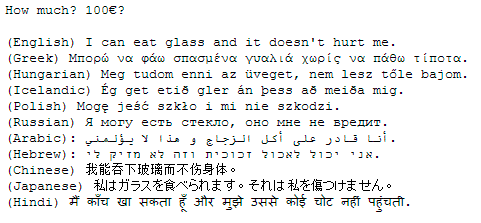
\includegraphics[scale=\NormalScale]{digging_into_code/strings/multilang_sampler.png}
\end{figure}

% FIXME: cut it
\begin{figure}[H]
\centering
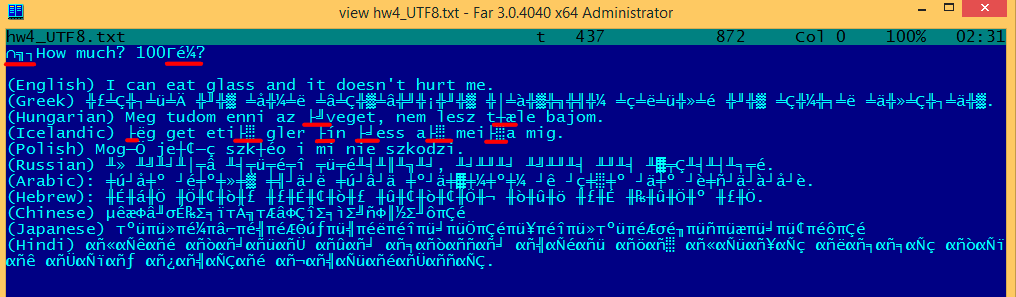
\includegraphics[scale=\FigScale]{digging_into_code/strings/multilang_sampler_UTF8.png}
\caption{FAR: UTF-8}
\end{figure}

As you can see, the English language string looks the same as it is in ASCII.

The Hungarian language uses some Latin symbols plus symbols with diacritic marks.

These symbols are encoded using several bytes, these are underscored with red.
It's the same story with the Icelandic and Polish languages.

There is also the \q{Euro} currency symbol at the start, which is encoded with 3 bytes.

The rest of the writing systems here have no connection with Latin.

At least in Russian, Arabic, Hebrew and Hindi we can see some recurring bytes, and that is not surprise:
all symbols from a writing system are usually located in the same Unicode table, so their code begins with
the same numbers.

At the beginning, before the \q{How much?} string we see 3 bytes, which are in fact the \ac{BOM}.
The \ac{BOM} defines the encoding system to be
used.

\subsubsection{UTF-16LE}

\myindex{UTF-16LE}
\myindex{Windows!Win32}
Many win32 functions in Windows have the suffixes \TT{-A} and \TT{-W}.
The first type of functions works
with normal strings, the other with UTF-16LE strings (\IT{wide}).

In the second case, each symbol is usually stored in a 16-bit value of type \IT{short}.

The Latin symbols in UTF-16 strings look in Hiew or FAR like they are interleaved with zero byte:

\begin{lstlisting}
int wmain()
{
	wprintf (L"Hello, world!\n");
};
\end{lstlisting}

\begin{figure}[H]
\centering
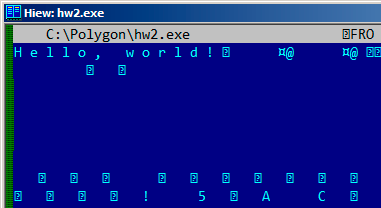
\includegraphics[scale=\NormalScale]{digging_into_code/strings/UTF16-string.png}
\caption{Hiew}
\end{figure}

We can see this often in \gls{Windows NT} system files:

\begin{figure}[H]
\centering
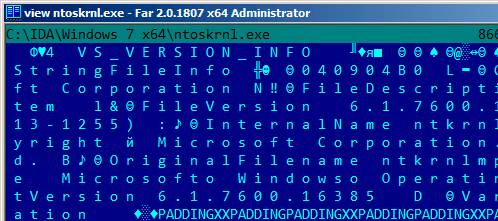
\includegraphics[scale=\NormalScale]{digging_into_code/strings/ntoskrnl_UTF16.png}
\caption{Hiew}
\end{figure}

\myindex{IDA}
Strings with characters that occupy exactly 2 bytes are called \q{Unicode} in \IDA:

\begin{lstlisting}
.data:0040E000 aHelloWorld:
.data:0040E000                 unicode 0, <Hello, world!>
.data:0040E000                 dw 0Ah, 0
\end{lstlisting}

Here is how the Russian language string is encoded in UTF-16LE:

\begin{figure}[H]
\centering
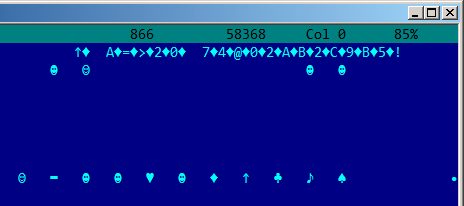
\includegraphics[scale=\NormalScale]{digging_into_code/strings/russian_UTF16.png}
\caption{Hiew: UTF-16LE}
\end{figure}

What we can easily spot is that the symbols are interleaved by the diamond character (which has the ASCII code of 4).
Indeed, the Cyrillic symbols are located in the fourth Unicode plane
\footnote{\href{http://go.yurichev.com/17003}{wikipedia}}.
Hence, all Cyrillic symbols in UTF-16LE are located in the \TT{0x400-0x4FF} range.

Let's go back to the example with the string written in multiple languages.
Here is how it looks like in UTF-16LE.

% FIXME: cut it
\begin{figure}[H]
\centering
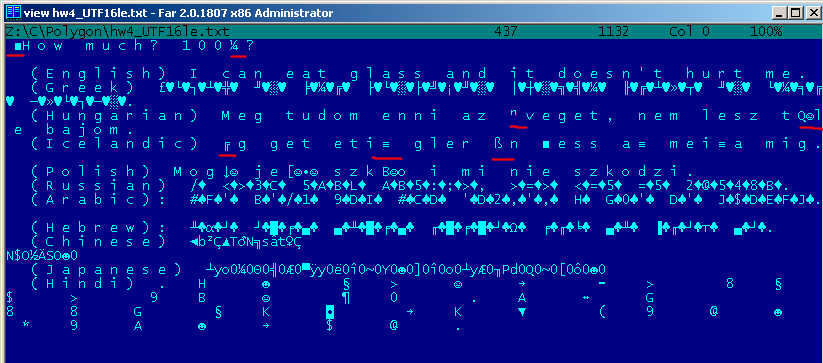
\includegraphics[scale=\FigScale]{digging_into_code/strings/multilang_sampler_UTF16.png}
\caption{FAR: UTF-16LE}
\end{figure}

Here we can also see the \ac{BOM} in the beginning.
All Latin characters are interleaved with a zero byte.

Some characters with diacritic marks (Hungarian and Icelandic languages) are also underscored in red.

% TODO: strings *NIX utility. procmonitor also shows strings...

% subsection:
\input{digging_into_code/strings/base64_EN}

}
\RU{\chapter{"Прикуп" в игре "Марьяж"}

\epigraph{Знал бы прикуп --- жил бы в Сочи.}{Поговорка.}

"Марьяж" --- старая и довольно популярная версия игры в "Преферанс" под DOS.

Играют три игрока, каждому раздается по 10 карт, остальные 2 остается в т.н. "прикупе".
Начинаются торги, во время которых "прикуп" скрыт.
Он открывается после того, как один из игроков сделает "заказ".

Знание карт в "прикупе" обычно имеет решающее преимущество.

Вот так в игре выглядит состояние "торгов", и "прикуп" посредине, скрытый:

\begin{figure}[H]
\centering
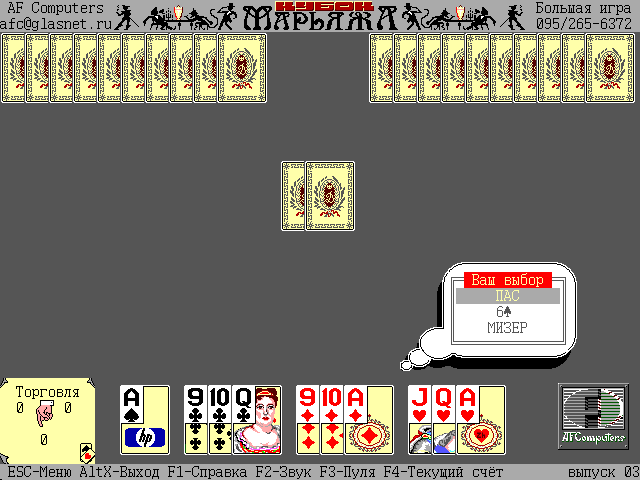
\includegraphics[scale=\FigScale]{examples/marriage/initial_not_patched.png}
\caption{"Торги"}
\end{figure}

Попробуем "подсмотреть" карты в "прикупе" в этой игре.

Для начала --- что мы знаем?
Игра под DOS, датируется 1997-м годом. IDA показывает имена стандартных функций вроде 
\TT{@GetImage\$q7Integert1t1t1m3Any} --- это "манглинг" типичный для Borland Pascal, что позволяет сделать вывод,
что сама игра написана на Паскале и скомпилирована Borland Pascal-ем.

Файлов около 10-и и некоторые имеют текстовую строку в заголовке "Marriage Image Library" --- вероятно,
это библиотеки спрайтов.

В IDA можно увидеть что используется функция \TT{@PutImage\$q7Integert1m3Any4Word}, которая, собственно,
рисует некий спрайт на экране.
Она вызывается по крайней мере из 8-и мест.
Чтобы узнать что происходит в каждом из этих 8-и мест, мы можем блокировать работу каждой функции и смотреть,
что будет происходить.
Например, первая ф-ция имеет адрес seg002:062E, и она заканчивается инструкцией \INS{retf 0Eh} на seg002:102A.
Это означает что метод вызовов ф-ций в Borland Pascal под DOS схож с stdcall --- вызываемая ф-ция должна сама
возвращать стек в состояние до того как началась передача аргументов.
В самом начале этой ф-ции вписываем инструкцию "retf 0eh", либо 3 байта: \TT{CA 0E 00}.
Запускаем "Марьяж" и внешне вроде бы ничего не изменилось.

Переходим ко второй ф-ции, которая активно использует \TT{@PutImage\$q7Integert1m3Any4Word}.
Она находится по адресу seg008:0AB5 и заканчивается инструкцией \INS{retf 0Ah}.
Вписываем эту инструкцию в самом начале и запускаем:

\begin{figure}[H]
\centering
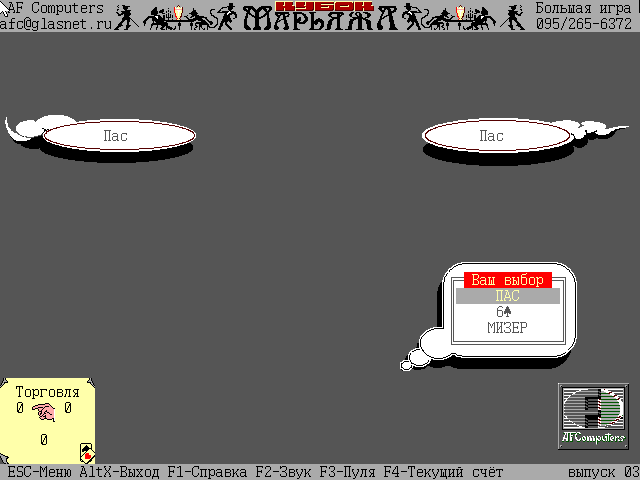
\includegraphics[scale=\FigScale]{examples/marriage/draw_card_bypass.png}
\caption{Карт нет}
\end{figure}

Карт не видно вообще. И видимо, эта функция их отображает, мы её заблокировали, и теперь карт не видно.
Назовем эту ф-цию в IDA \TT{draw\_card()}.
Помимо \TT{@PutImage\$q7Integert1m3Any4Word}, в этой ф-ции вызываются также ф-ции @SetColor\$q4Word, 
\TT{@SetFillStyle\$q4Wordt1}, \TT{@Bar\$q7Integert1t1t1}, \TT{@OutTextXY\$q7Integert16String}.

Сама ф-ция \TT{draw\_cards()} (её название мы дали ей сами только что) вызывается из 4-х мест.
Попробуем точно также "блокировать" каждую ф-цию.

Когда я "блокирую" вторую, по адресу seg008:0DF3 и запускаю программу, вижу такое:

\begin{figure}[H]
\centering
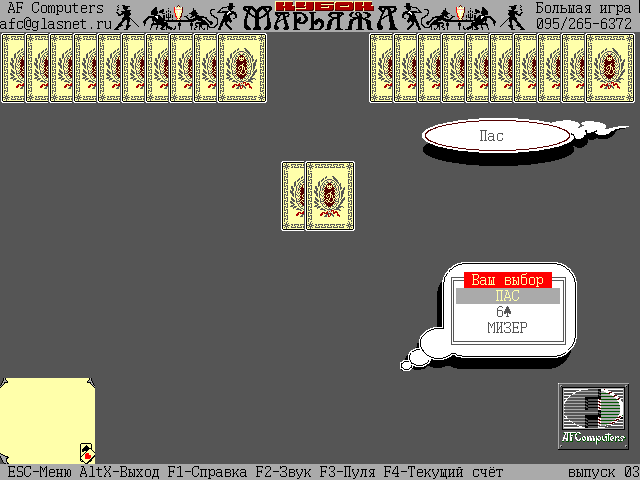
\includegraphics[scale=\FigScale]{examples/marriage/draw_players_cards.png}
\caption{Все карты кроме карт игрока}
\end{figure}

Видны все карты, кроме карт игрока. Видимо, эта функция рисует карты игрока. \\
Я переименовываю её в IDA в \TT{draw\_players\_cards()}.

Четвертая ф-ция, вызывающая \TT{draw\_cards()}, находится по адресу seg008:16B3, и когда я её "блокирую",
я вижу в игре такое:

\begin{figure}[H]
\centering
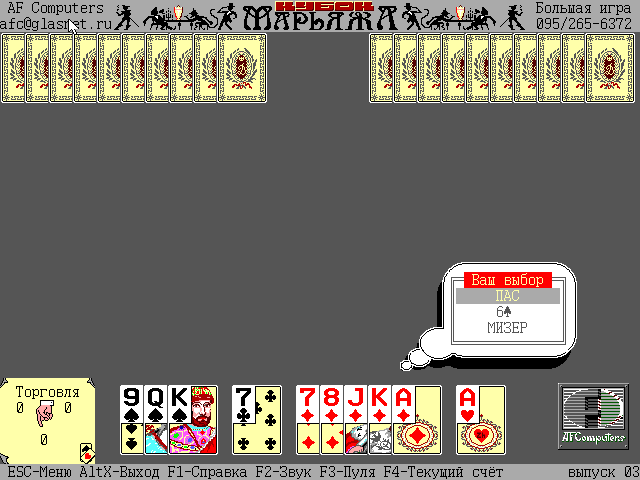
\includegraphics[scale=\FigScale]{examples/marriage/no_prikup.png}
\caption{"Прикупа" нет}
\end{figure}

Все карты есть, кроме "прикупа". Более того, эта ф-ция вызывает только \TT{draw\_cards()}, и только 2 раза.
Видимо эта ф-ция и отображает карты "прикупа".
Будем рассматривать её внимательнее.

\begin{lstlisting}
seg008:16B3 draw_prikup     proc far                ; CODE XREF: seg010:00B0
seg008:16B3                                         ; sub_15098+6
seg008:16B3
seg008:16B3 var_E           = word ptr -0Eh
seg008:16B3 var_C           = word ptr -0Ch
seg008:16B3 arg_0           = byte ptr  6
seg008:16B3
seg008:16B3                 enter   0Eh, 0
seg008:16B7                 mov     al, byte_2C0EA
seg008:16BA                 xor     ah, ah
seg008:16BC                 imul    ax, 23h
seg008:16BF                 mov     [bp+var_C], ax
seg008:16C2                 mov     al, byte_2C0EB
seg008:16C5                 xor     ah, ah
seg008:16C7                 imul    ax, 0Ah
seg008:16CA                 mov     [bp+var_E], ax
seg008:16CD                 cmp     [bp+arg_0], 0
seg008:16D1                 jnz     short loc_1334A
seg008:16D3                 cmp     byte_2BB08, 0
seg008:16D8                 jz      short loc_13356
seg008:16DA
seg008:16DA loc_1334A:                              ; CODE XREF: draw_prikup+1E
seg008:16DA                 mov     al, byte ptr word_32084
seg008:16DD                 mov     byte_293AD, al
seg008:16E0                 mov     al, byte ptr word_32086
seg008:16E3                 mov     byte_293AC, al
seg008:16E6
seg008:16E6 loc_13356:                              ; CODE XREF: draw_prikup+25
seg008:16E6                 mov     al, byte_293AC
seg008:16E9                 xor     ah, ah
seg008:16EB                 push    ax
seg008:16EC                 mov     al, byte_293AD
seg008:16EF                 xor     ah, ah
seg008:16F1                 push    ax
seg008:16F2                 push    [bp+var_C]
seg008:16F5                 push    [bp+var_E]
seg008:16F8                 cmp     [bp+arg_0], 0
seg008:16FC                 jnz     short loc_13379
seg008:16FE                 cmp     byte_2BB08, 0
seg008:1703                 jnz     short loc_13379
seg008:1705                 mov     al, 0
seg008:1707                 jmp     short loc_1337B
seg008:1709 ; ---------------------------------------------------------------------------
seg008:1709
seg008:1709 loc_13379:                              ; CODE XREF: draw_prikup+49
seg008:1709                                         ; draw_prikup+50
seg008:1709                 mov     al, 1
seg008:170B
seg008:170B loc_1337B:                              ; CODE XREF: draw_prikup+54
seg008:170B                 push    ax
seg008:170C                 push    cs
seg008:170D                 call    near ptr draw_card
seg008:1710                 mov     al, byte_2C0EA
seg008:1713                 xor     ah, ah
seg008:1715                 mov     si, ax
seg008:1717                 shl     ax, 1
seg008:1719                 add     ax, si
seg008:171B                 add     ax, [bp+var_C]
seg008:171E                 mov     [bp+var_C], ax
seg008:1721                 cmp     [bp+arg_0], 0
seg008:1725                 jnz     short loc_1339E
seg008:1727                 cmp     byte_2BB08, 0
seg008:172C                 jz      short loc_133AA
seg008:172E
seg008:172E loc_1339E:                              ; CODE XREF: draw_prikup+72
seg008:172E                 mov     al, byte ptr word_32088
seg008:1731                 mov     byte_293AD, al
seg008:1734                 mov     al, byte ptr word_3208A
seg008:1737                 mov     byte_293AC, al
seg008:173A
seg008:173A loc_133AA:                              ; CODE XREF: draw_prikup+79
seg008:173A                 mov     al, byte_293AC
seg008:173D                 xor     ah, ah
seg008:173F                 push    ax
seg008:1740                 mov     al, byte_293AD
seg008:1743                 xor     ah, ah
seg008:1745                 push    ax
seg008:1746                 push    [bp+var_C]
seg008:1749                 push    [bp+var_E]
seg008:174C                 cmp     [bp+arg_0], 0
seg008:1750                 jnz     short loc_133CD
seg008:1752                 cmp     byte_2BB08, 0
seg008:1757                 jnz     short loc_133CD
seg008:1759                 mov     al, 0
seg008:175B                 jmp     short loc_133CF
seg008:175D ; ---------------------------------------------------------------------------
seg008:175D
seg008:175D loc_133CD:                              ; CODE XREF: draw_prikup+9D
seg008:175D                                         ; draw_prikup+A4
seg008:175D                 mov     al, 1
seg008:175F
seg008:175F loc_133CF:                              ; CODE XREF: draw_prikup+A8
seg008:175F                 push    ax
seg008:1760                 push    cs
seg008:1761                 call    near ptr draw_card ; prikup #2
seg008:1764                 leave
seg008:1765                 retf    2
seg008:1765 draw_prikup     endp
\end{lstlisting}

Интересно посмотреть, как именно вызывается \TT{draw\_prikup()}. У нее только один аргумент.

Иногда она вызывается с аргументом 1:

\begin{lstlisting}
...
seg010:084C                 push    1
seg010:084E                 call    draw_prikup
...
\end{lstlisting}

А иногда с аргументом 0, причем вот в таком контексте, где уже есть другая знакомая функция:

\begin{lstlisting}
seg010:0067                 push    1
seg010:0069                 mov     al, byte_31F41
seg010:006C                 push    ax
seg010:006D                 call    sub_12FDC
seg010:0072                 push    1
seg010:0074                 mov     al, byte_31F41
seg010:0077                 push    ax
seg010:0078                 call    draw_players_cards
seg010:007D                 push    2
seg010:007F                 mov     al, byte_31F42
seg010:0082                 push    ax
seg010:0083                 call    sub_12FDC
seg010:0088                 push    2
seg010:008A                 mov     al, byte_31F42
seg010:008D                 push    ax
seg010:008E                 call    draw_players_cards
seg010:0093                 push    3
seg010:0095                 mov     al, byte_31F43
seg010:0098                 push    ax
seg010:0099                 call    sub_12FDC
seg010:009E                 push    3
seg010:00A0                 mov     al, byte_31F43
seg010:00A3                 push    ax
seg010:00A4                 call    draw_players_cards
seg010:00A9                 call    sub_1257A
seg010:00AE                 push    0
seg010:00B0                 call    draw_prikup
seg010:00B5                 mov     byte_2BB95, 0
\end{lstlisting}

Так что единственный аргумент у \TT{draw\_prikup()} может быть или 0 или 1, т.е., это, возможно, булевый тип.
На что он влияет внутри самой ф-ции?
При ближайшем рассмотрении видно, что входящий 0 или 1 передается в \TT{draw\_card()}, т.е., у последней тоже есть
булевый аргумент.
Помимо всего прочего, если передается 1, то по адресам seg008:16DA и seg008:172E копируются несколько байт
из одной группы глобальных переменных в другую.

Эксперимент: здесь 4 раза сравнивается единственный аргумент с 0 и далее следует \INS{JNZ}.
Что если сравнение будет происходит с 1, и, таким образом, работа функции \TT{draw\_prikup()} будет обратной?
Патчим и запускаем:

\begin{figure}[H]
\centering
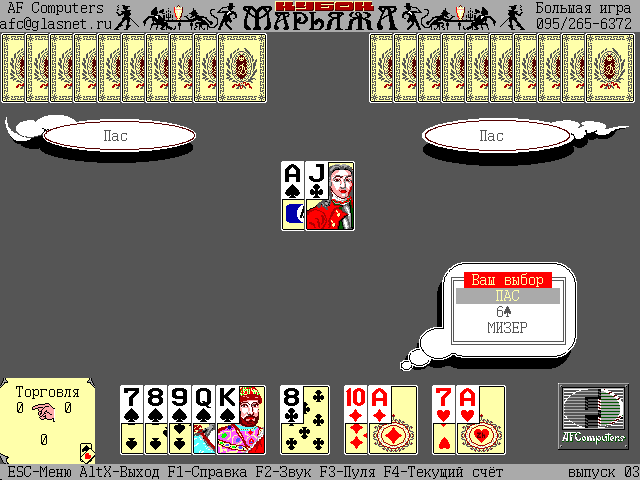
\includegraphics[scale=\FigScale]{examples/marriage/patch1.png}
\caption{"Прикуп" открыт}
\end{figure}

"Прикуп" открыт, но когда я делаю "заказ", и, по логике вещей, "прикуп" теперь должен стать открытым,
он наоборот становится закрытым:

\begin{figure}[H]
\centering
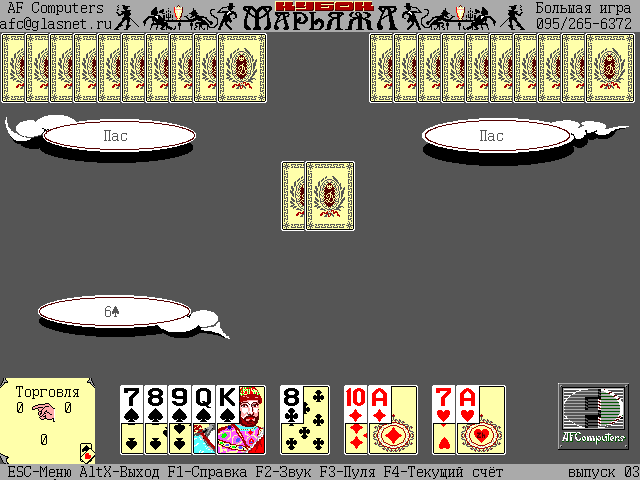
\includegraphics[scale=\FigScale]{examples/marriage/patch2.png}
\caption{"Прикуп" закрыт}
\end{figure}

Всё ясно: если аргумент \TT{draw\_prikup()} нулевой, то карты рисуются рубашкой вверх, если 1, то открытые.
Этот же аргумент передается в \TT{draw\_card()} --- эта ф-ция может рисовать и открытые и закрытые карты.

Пропатчить "Марьяж" теперь легко, достаточно исправить все условные переходы так, как будто бы в ф-цию
всегда приходит 1 в аргументе и тогда "прикуп" всегда будет открыт.

Но что за байты копируются в seg008:16DA и seg008:172E?
Я попробовал забить инструкции копирования \MOV \NOP{}-ами --- "прикуп" вообще перестал отображаться.

Тогда я сделал так, чтобы всегда записывалась 1:

\begin{lstlisting}
...
00004B5A: B001                           mov         al,1
00004B5C: 90                             nop
00004B5D: A26D08                         mov         [0086D],al
00004B60: B001                           mov         al,1
00004B62: 90                             nop
00004B63: A26C08                         mov         [0086C],al
...
\end{lstlisting}

Тогда "прикуп" отображается как два пиковых туза.
А если первый байт --- 2, а второй --- 1, получается трефовый туз.
Видимо так и кодируется масть карты, а затем и сама карта.
% TODO \ref{} сюда о том, как можно передавать аргументы в глоб.переменных
А \TT{draw\_card()} затем считывает эту информацию из пары глобальных переменных.
А копируется она тоже из глобальных переменных, где собственно и находится состояние карт у игроков и в прикупе
после случайной тасовки.
Но нельзя забывать что если мы сделаем так, что в "прикупе" всегда будет 2 пиковых туза, это будет только
на экране так отображаться, а в памяти состояние карт останется таким же, как и после тасовки.

Я также пробовал сделать пранк: во время торгов одна карта "прикупа" открыта, а вторая закрыта, а после "заказа",
наоборот, первая закрыта, а вторая открывается. В качестве упражнения, вы можете попробовать сделать так.

Еще кое-что: чтобы сделать прикуп открытым, ведь можно же найти место где вызывается \TT{draw\_prikup()} и поменять 0
на 1. Можно, только это место не в головой marriage.exe, а в marriage.000, а это DOS-овский оверлей (начинается
с сигнатуры "FBOV").

В качестве упражнения, можно попробовать подсматривать состояние всех карт, и у обоих игроков.
Для этого нужно отладчиком смотреть состояние глобальной памяти рядом с тем, откуда считываются обе карты
прикупа.

Файлы: \\
оригинальная версия: \url{http://beginners.re/examples/marriage/original.zip}, \\
пропатченная мною версия: \url{http://beginners.re/examples/marriage/patched.zip} 
(все 4 условных перехода после \TT{cmp [bp+arg\_0], 0} заменены на \JMP).

}

\renewcommand{\CURPATH}{advanced/102_fib}
\chapter{\RU{Конверсия строки в число}\EN{String to number conversion} (atoi())}

\myindex{\CStandardLibrary!atoi()}
\RU{Попробуем реализовать стандарту функцию Си atoi().}
\EN{Let's try to reimplement the standard atoi() C function.}

\section{\RU{Простой пример}\EN{Simple example}}

\RU{Это самый простой способ прочитать число, представленное в кодировке \ac{ASCII}.}
\EN{Here is the simplest possible way to read a number represented in \ac{ASCII} encoding.}
\RU{Он не защищен от ошибок: символ отличный от цифры приведет к неверному результату.}
\EN{It's not error-prone: a character other than a digit leads to incorrect result.}

\lstinputlisting{\CURPATH/atoi.c}

\RU{То, что делает алгоритм это просто считывает цифры слева направо.}
\EN{So what the algorithm does is just reading digits from left to right.}
\RU{Символ нуля в \ac{ASCII} вычитается из каждой цифры.}
\EN{The zero \ac{ASCII} character is subtracted from each digit. }
\RU{Цифры от \q{0} до \q{9} расположены по порядку в таблице \ac{ASCII}, так что мы даже можем
и не знать точного значения символа \q{0}.}
\EN{The digits from \q{0} to \q{9} are consecutive in the \ac{ASCII} table, so 
we do not even need to know the exact value of the \q{0} character.}
\RU{Всё что нам нужно знать это то что \q{0} минус \q{0}\EMDASH{}это 0, а \q{9} минус \q{0} это 9, \etc{}.}
\EN{All we need to know is that \q{0} minus \q{0} is 0, \q{9} minus \q{0}'is 9 and so on.}
\RU{Вычитание \q{0} от каждого символа в итоге дает число от 0 до 9 включительно.}
\EN{Subtracting \q{0} from each character results in a number from 0 to 9 inclusive.}
\RU{Любой другой символ, конечно, приведет к неверному результату!}
\EN{Any other character leads to an incorrect result, of course!}
\RU{Каждая цифра добавляется к итоговому результату (в переменной \q{rt}), но итоговый результат
также умножается на 10 на каждой цифре.}
\EN{Each digit has to be added to the final result (in variable \q{rt}), but the final result
is also multiplied by 10 at each digit.}
\RU{Другими словами, на каждой итерации, результат сдвигается влево на одну позицию в десятичном виде.}
\EN{In other words, the result is shifted left by one position in decimal form on each iteration.}
\RU{Самая последняя цифра прибавляется, но не сдвигается.}
\EN{The last digit is added, but there is no no shift.}

\subsection{\Optimizing MSVC 2013 x64}

\lstinputlisting[caption=\Optimizing MSVC 2013 x64]{\CURPATH/atoi.asm.MSVC2013.x64.Ox.\LANG}

\RU{Символы загружаются в двух местах: первый символ и все последующие символы.}
\EN{A character can be loaded in two places: the first character and all subsequent characters.}
\RU{Это сделано для перегруппировки цикла.}\EN{This is done for loop regrouping.}
\myindex{x86!\Instructions!LEA}
\RU{Здесь нет инструкции для умножения на 10, вместо этого две LEA делают это же.}
\EN{There is no instruction for multiplication by 10, two LEA instruction do this instead.}
\myindex{x86!\Instructions!ADD}
\myindex{x86!\Instructions!SUB}
\RU{MSVC иногда использует инструкцию ADD с отрицательной константой вместо SUB.}
\EN{MSVC sometimes uses the ADD instruction with a negative constant instead of SUB.}
\RU{Это тот случай}\EN{This is the case}.
\RU{Честно говоря, трудно сказать, чем это лучше, чем SUB.}
\EN{It's very hard to say why this is better then SUB.}
\RU{Но MSVC делает так часто}\EN{But MSVC does this often}.

\subsection{\Optimizing GCC 4.9.1 x64}

\Optimizing GCC 4.9.1 \RU{более краток, но здесь есть одна лишняя инструкция RET в конце.}
\EN{is more concise, but there is one redundant RET instruction at the end.}
\RU{Одной было бы достаточно}\EN{One would be enough}.

\lstinputlisting[caption=\Optimizing GCC 4.9.1 x64]{\CURPATH/atoi.s.GCC491.O3.x64.\LANG}

\subsection{\OptimizingKeilVI (\ARMMode)}

\lstinputlisting[caption=\OptimizingKeilVI (\ARMMode)]{\CURPATH/atoi.s.ARM.O3.\LANG}

\subsection{\OptimizingKeilVI (\ThumbMode)}

\lstinputlisting[caption=\OptimizingKeilVI (\ThumbMode)]{\CURPATH/atoi.s.thumb.O3.\LANG}

\RU{Интересно, из школьного курса математики мы можем помнить что порядок операций сложения и вычитания
не играет роли.}
\EN{Interestingly, from school mathematics we may remember that the order of addition and 
subtraction operations doesn't matter.}
\RU{Это наш случай: в начале вычисляется выражение $rt*10 - '0'$, затем к нему прибавляется 
значение входного символа.}
\EN{That's our case: first, the $rt*10 - '0'$ expression is computed, then the input character value 
is added to it.}
\RU{Действительно, результат тот же, но компилятор немного всё перегруппировал.}
\EN{Indeed, the result is the same, but the compiler did some regrouping.}

\subsection{\Optimizing GCC 4.9.1 ARM64}

\RU{Компилятор для ARM64 может использовать суффикс инструкции, задающий пре-инкремент:}
\EN{The ARM64 compiler can use the pre-increment instruction suffix:}

\lstinputlisting[caption=\Optimizing GCC 4.9.1 ARM64]{\CURPATH/atoi.s.GCC49.ARM64.O3.\LANG}

\section{\RU{Немного расширенный пример}\EN{A slightly advanced example}}

\RU{Новый пример более расширенный, теперь здесь есть проверка знака \q{минус} в самом начале,
и еще он может сообщать об ошибке если не-цифра была найдена во входной строке:}
\EN{My new code snippet is more advanced, now it checks for the \q{minus} sign at the first character
and reports an error if a non-digit was found in the input string:}

\lstinputlisting{\CURPATH/atoi2.c}

\subsection{\Optimizing GCC 4.9.1 x64}

\lstinputlisting[caption=\Optimizing GCC 4.9.1 x64]{\CURPATH/atoi2.s.GCC491.O3.x64.\LANG}

\myindex{x86!\Instructions!NEG}
\RU{Если знак \q{минус} был найден в начале строки, инструкция NEG будет исполнена в конце.}
\EN{If the \q{minus} sign was encountered at the string start, the NEG instruction is to be executed at the end.}
\RU{Она просто меняет знак числа}\EN{It just negates the number}.

\label{one_comparison_instead_of_two}
\RU{Еще кое-что надо отметить}\EN{There is one more thing that needs mentioning}.
\RU{Как среднестатистический программист будет проверять, является ли символ цифрой?}
\EN{How would a common programmer check if the character is not a digit?}
\RU{Так же, как и у нас в исходном коде}\EN{Just how we have it in the source code}:

\begin{lstlisting}
if (*s<'0' || *s>'9')
    ...
\end{lstlisting}

\RU{Здесь две операции сравнения}\EN{There are two comparison operations}.
\RU{Но что интересно, так это то что мы можем заменить обе операции на одну:}
\EN{What is interesting is that we can replace both operations by single one:}
\RU{просто вычитайте \q{0} из значения символа}\EN{just subtract \q{0} from character value},
\RU{считается результат за беззнаковое значение (это важно) и проверьте, не больше ли он чем 9.}
\EN{treat result as unsigned value (this is important) and check if it's greater than 9.}

\RU{Например, скажем, строка на входе имеет символ точки (\q{.}), которая имеет код 46 в таблице \ac{ASCII}.}
\EN{For example, let's say that the user input contains the dot character (\q{.}) which has \ac{ASCII} code 46.}
$46-48=-2$ \RU{если считать результат за знаковое число}\EN{if we treat the result as a signed number}.
\RU{Действительно, символ точки расположен на два места раньше, чем символ \q{0} в таблице \ac{ASCII}.}
\EN{Indeed, the dot character is located two places earlier than the \q{0} character in the \ac{ASCII} table.}
\RU{Но это}\EN{But it is} \TT{0xFFFFFFFE} (4294967294) \RU{если считать результат за беззнаковое значение, 
и это точно больше чем 9!}
\EN{if we treat the result as an unsigned value, and that's definitely bigger than 9!}

\RU{Компиляторы часто так делают, важно распознавать эти трюки.}
\EN{The compilers do this often, so it's important to recognize these tricks.}

\EN{Another example of it in this book}\RU{Еще один пример подобного в этой книге}: 
\myref{toupper_one_comparison}.

\Optimizing MSVC 2013 x64 \RU{применяет те же трюки}\EN{does the same tricks}.

\subsection{\OptimizingKeilVI (\ARMMode)}

\lstinputlisting[caption=\OptimizingKeilVI (\ARMMode),numbers=left]{\CURPATH/atoi2.s.ARM.O3.\LANG}

\RU{В 32-битном ARM нет инструкции NEG, так что вместо этого используется операция \q{Reverse Subtraction}
(строка 31).}
\EN{There is no NEG instruction in 32-bit ARM, so the \q{Reverse Subtraction} operation (line 31) 
is used here.}
\RU{Она сработает если результат инструкции CMP (на строке 29) был \q{Not Equal} 
(не равно, отсюда суффикс -NE suffix).}
\EN{It is triggered if the result of the CMP instruction (at line 29) was \q{Not Equal} (hence -NE suffix).}
\myindex{ARM!\Instructions!RSB}
\RU{Что делает RSBNE это просто вычитает результирующее значение из нуля.}
\EN{So what RSBNE does is to subtract the resulting value from 0.}
\RU{Она работает, как и обычное вычитание, но меняет местами операнды.}
\EN{It works just like the regular subtraction operation, but swaps operands.}
\RU{Вычитание любого числа из нуля это смена знака}
\EN{Subtracting any number from 0 results in negation}: $0-x=-x$.

\RU{Код для режима Thumb почти такой же.}
\EN{Thumb mode code is mostly the same.}

\myindex{ARM!\Instructions!NEG}
GCC 4.9 \ForENRU ARM64 \RU{может использовать инструкцию NEG, доступную в}
\EN{can use the NEG instruction, which is available in} ARM64.

\section{\Exercise{}}

\myindex{Fuzzing}
\EN{Oh, by the way, security researchers deals often with unpredictable behaviour of program while handling of incorrect data.}
\RU{Кстати, security research-еры часто имеют дело с непредсказуемым поведением программ во время обработки некорректных данных.}
\RU{Например, во время fuzzing-а.}
\EN{For example, while fuzzing.}
\EN{As an exercise, you may try to enter non-digit characters and see what happens.}
\RU{В качестве упражнения, вы можете попробовать ввести символы не относящиеся к числам и посмотреть, что случится.}
\EN{Try to explain, what happened and why.}
\RU{Попробуйте объяснить, что произошло, и почему.}




\renewcommand{\CURPATH}{advanced/110_CRC32}
\EN{\section{Text strings}

\subsection{\CCpp}

\label{C_strings}
The normal C strings are zero-terminated (\ac{ASCIIZ}-strings).

The reason why the C string format is as it is (zero-terminated) is apparently historical.
In [Dennis M. Ritchie, \IT{The Evolution of the Unix Time-sharing System}, (1979)]
we read:

\begin{framed}
\begin{quotation}
A minor difference was that the unit of I/O was the word, not the byte, because the PDP-7 was a word-addressed
machine. In practice this meant merely that all programs dealing with character streams ignored null
characters, because null was used to pad a file to an even number of characters.
\end{quotation}
\end{framed}

\myindex{Hiew}

In Hiew or FAR Manager these strings looks like this:

\begin{lstlisting}
int main()
{
	printf ("Hello, world!\n");
};
\end{lstlisting}

\begin{figure}[H]
\centering
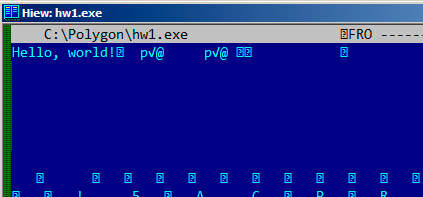
\includegraphics[scale=\NormalScale]{digging_into_code/strings/C-string.png}
\caption{Hiew}
\end{figure}

% FIXME видно \n в конце, потом пробел

\subsection{Borland Delphi}
\myindex{Pascal}
\myindex{Borland Delphi}

The string in Pascal and Borland Delphi is preceded by an 8-bit or 32-bit string length.

For example:

\begin{lstlisting}[caption=Delphi]
CODE:00518AC8                 dd 19h
CODE:00518ACC aLoading___Plea db 'Loading... , please wait.',0

...

CODE:00518AFC                 dd 10h
CODE:00518B00 aPreparingRun__ db 'Preparing run...',0
\end{lstlisting}

\subsection{Unicode}

\myindex{Unicode}

Often, what is called Unicode is a methods for encoding strings where each character occupies 2 bytes or 16 bits.
This is a common terminological mistake.
Unicode is a standard for assigning a number to each character in the many writing systems of the 
world, but does not describe the encoding method.

\myindex{UTF-8}
\myindex{UTF-16LE}
The most popular encoding methods are: UTF-8 (is widespread in Internet and *NIX systems) and UTF-16LE (is used in Windows).

\subsubsection{UTF-8}

\myindex{UTF-8}
UTF-8 is one of the most successful methods for
encoding characters.
All Latin symbols are encoded just like in ASCII,
and the symbols beyond the ASCII table are encoded using several bytes.
0 is encoded as
before, so all standard C string functions work with UTF-8 strings just like any other string.

Let's see how the symbols in various languages are encoded in UTF-8 and how it looks like in FAR, using the 437 codepage
\footnote{The example and translations was taken from here: 
\url{http://go.yurichev.com/17304}}:

\begin{figure}[H]
\centering
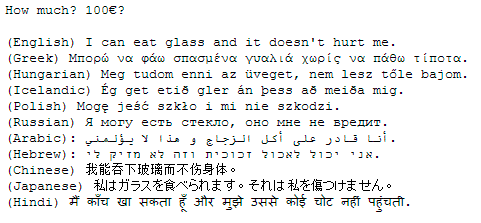
\includegraphics[scale=\NormalScale]{digging_into_code/strings/multilang_sampler.png}
\end{figure}

% FIXME: cut it
\begin{figure}[H]
\centering
\includegraphics[scale=\FigScale]{digging_into_code/strings/multilang_sampler_UTF8.png}
\caption{FAR: UTF-8}
\end{figure}

As you can see, the English language string looks the same as it is in ASCII.

The Hungarian language uses some Latin symbols plus symbols with diacritic marks.

These symbols are encoded using several bytes, these are underscored with red.
It's the same story with the Icelandic and Polish languages.

There is also the \q{Euro} currency symbol at the start, which is encoded with 3 bytes.

The rest of the writing systems here have no connection with Latin.

At least in Russian, Arabic, Hebrew and Hindi we can see some recurring bytes, and that is not surprise:
all symbols from a writing system are usually located in the same Unicode table, so their code begins with
the same numbers.

At the beginning, before the \q{How much?} string we see 3 bytes, which are in fact the \ac{BOM}.
The \ac{BOM} defines the encoding system to be
used.

\subsubsection{UTF-16LE}

\myindex{UTF-16LE}
\myindex{Windows!Win32}
Many win32 functions in Windows have the suffixes \TT{-A} and \TT{-W}.
The first type of functions works
with normal strings, the other with UTF-16LE strings (\IT{wide}).

In the second case, each symbol is usually stored in a 16-bit value of type \IT{short}.

The Latin symbols in UTF-16 strings look in Hiew or FAR like they are interleaved with zero byte:

\begin{lstlisting}
int wmain()
{
	wprintf (L"Hello, world!\n");
};
\end{lstlisting}

\begin{figure}[H]
\centering
\includegraphics[scale=\NormalScale]{digging_into_code/strings/UTF16-string.png}
\caption{Hiew}
\end{figure}

We can see this often in \gls{Windows NT} system files:

\begin{figure}[H]
\centering
\includegraphics[scale=\NormalScale]{digging_into_code/strings/ntoskrnl_UTF16.png}
\caption{Hiew}
\end{figure}

\myindex{IDA}
Strings with characters that occupy exactly 2 bytes are called \q{Unicode} in \IDA:

\begin{lstlisting}
.data:0040E000 aHelloWorld:
.data:0040E000                 unicode 0, <Hello, world!>
.data:0040E000                 dw 0Ah, 0
\end{lstlisting}

Here is how the Russian language string is encoded in UTF-16LE:

\begin{figure}[H]
\centering
\includegraphics[scale=\NormalScale]{digging_into_code/strings/russian_UTF16.png}
\caption{Hiew: UTF-16LE}
\end{figure}

What we can easily spot is that the symbols are interleaved by the diamond character (which has the ASCII code of 4).
Indeed, the Cyrillic symbols are located in the fourth Unicode plane
\footnote{\href{http://go.yurichev.com/17003}{wikipedia}}.
Hence, all Cyrillic symbols in UTF-16LE are located in the \TT{0x400-0x4FF} range.

Let's go back to the example with the string written in multiple languages.
Here is how it looks like in UTF-16LE.

% FIXME: cut it
\begin{figure}[H]
\centering
\includegraphics[scale=\FigScale]{digging_into_code/strings/multilang_sampler_UTF16.png}
\caption{FAR: UTF-16LE}
\end{figure}

Here we can also see the \ac{BOM} in the beginning.
All Latin characters are interleaved with a zero byte.

Some characters with diacritic marks (Hungarian and Icelandic languages) are also underscored in red.

% TODO: strings *NIX utility. procmonitor also shows strings...

% subsection:
\input{digging_into_code/strings/base64_EN}

}
\RU{\chapter{"Прикуп" в игре "Марьяж"}

\epigraph{Знал бы прикуп --- жил бы в Сочи.}{Поговорка.}

"Марьяж" --- старая и довольно популярная версия игры в "Преферанс" под DOS.

Играют три игрока, каждому раздается по 10 карт, остальные 2 остается в т.н. "прикупе".
Начинаются торги, во время которых "прикуп" скрыт.
Он открывается после того, как один из игроков сделает "заказ".

Знание карт в "прикупе" обычно имеет решающее преимущество.

Вот так в игре выглядит состояние "торгов", и "прикуп" посредине, скрытый:

\begin{figure}[H]
\centering
\includegraphics[scale=\FigScale]{examples/marriage/initial_not_patched.png}
\caption{"Торги"}
\end{figure}

Попробуем "подсмотреть" карты в "прикупе" в этой игре.

Для начала --- что мы знаем?
Игра под DOS, датируется 1997-м годом. IDA показывает имена стандартных функций вроде 
\TT{@GetImage\$q7Integert1t1t1m3Any} --- это "манглинг" типичный для Borland Pascal, что позволяет сделать вывод,
что сама игра написана на Паскале и скомпилирована Borland Pascal-ем.

Файлов около 10-и и некоторые имеют текстовую строку в заголовке "Marriage Image Library" --- вероятно,
это библиотеки спрайтов.

В IDA можно увидеть что используется функция \TT{@PutImage\$q7Integert1m3Any4Word}, которая, собственно,
рисует некий спрайт на экране.
Она вызывается по крайней мере из 8-и мест.
Чтобы узнать что происходит в каждом из этих 8-и мест, мы можем блокировать работу каждой функции и смотреть,
что будет происходить.
Например, первая ф-ция имеет адрес seg002:062E, и она заканчивается инструкцией \INS{retf 0Eh} на seg002:102A.
Это означает что метод вызовов ф-ций в Borland Pascal под DOS схож с stdcall --- вызываемая ф-ция должна сама
возвращать стек в состояние до того как началась передача аргументов.
В самом начале этой ф-ции вписываем инструкцию "retf 0eh", либо 3 байта: \TT{CA 0E 00}.
Запускаем "Марьяж" и внешне вроде бы ничего не изменилось.

Переходим ко второй ф-ции, которая активно использует \TT{@PutImage\$q7Integert1m3Any4Word}.
Она находится по адресу seg008:0AB5 и заканчивается инструкцией \INS{retf 0Ah}.
Вписываем эту инструкцию в самом начале и запускаем:

\begin{figure}[H]
\centering
\includegraphics[scale=\FigScale]{examples/marriage/draw_card_bypass.png}
\caption{Карт нет}
\end{figure}

Карт не видно вообще. И видимо, эта функция их отображает, мы её заблокировали, и теперь карт не видно.
Назовем эту ф-цию в IDA \TT{draw\_card()}.
Помимо \TT{@PutImage\$q7Integert1m3Any4Word}, в этой ф-ции вызываются также ф-ции @SetColor\$q4Word, 
\TT{@SetFillStyle\$q4Wordt1}, \TT{@Bar\$q7Integert1t1t1}, \TT{@OutTextXY\$q7Integert16String}.

Сама ф-ция \TT{draw\_cards()} (её название мы дали ей сами только что) вызывается из 4-х мест.
Попробуем точно также "блокировать" каждую ф-цию.

Когда я "блокирую" вторую, по адресу seg008:0DF3 и запускаю программу, вижу такое:

\begin{figure}[H]
\centering
\includegraphics[scale=\FigScale]{examples/marriage/draw_players_cards.png}
\caption{Все карты кроме карт игрока}
\end{figure}

Видны все карты, кроме карт игрока. Видимо, эта функция рисует карты игрока. \\
Я переименовываю её в IDA в \TT{draw\_players\_cards()}.

Четвертая ф-ция, вызывающая \TT{draw\_cards()}, находится по адресу seg008:16B3, и когда я её "блокирую",
я вижу в игре такое:

\begin{figure}[H]
\centering
\includegraphics[scale=\FigScale]{examples/marriage/no_prikup.png}
\caption{"Прикупа" нет}
\end{figure}

Все карты есть, кроме "прикупа". Более того, эта ф-ция вызывает только \TT{draw\_cards()}, и только 2 раза.
Видимо эта ф-ция и отображает карты "прикупа".
Будем рассматривать её внимательнее.

\begin{lstlisting}
seg008:16B3 draw_prikup     proc far                ; CODE XREF: seg010:00B0
seg008:16B3                                         ; sub_15098+6
seg008:16B3
seg008:16B3 var_E           = word ptr -0Eh
seg008:16B3 var_C           = word ptr -0Ch
seg008:16B3 arg_0           = byte ptr  6
seg008:16B3
seg008:16B3                 enter   0Eh, 0
seg008:16B7                 mov     al, byte_2C0EA
seg008:16BA                 xor     ah, ah
seg008:16BC                 imul    ax, 23h
seg008:16BF                 mov     [bp+var_C], ax
seg008:16C2                 mov     al, byte_2C0EB
seg008:16C5                 xor     ah, ah
seg008:16C7                 imul    ax, 0Ah
seg008:16CA                 mov     [bp+var_E], ax
seg008:16CD                 cmp     [bp+arg_0], 0
seg008:16D1                 jnz     short loc_1334A
seg008:16D3                 cmp     byte_2BB08, 0
seg008:16D8                 jz      short loc_13356
seg008:16DA
seg008:16DA loc_1334A:                              ; CODE XREF: draw_prikup+1E
seg008:16DA                 mov     al, byte ptr word_32084
seg008:16DD                 mov     byte_293AD, al
seg008:16E0                 mov     al, byte ptr word_32086
seg008:16E3                 mov     byte_293AC, al
seg008:16E6
seg008:16E6 loc_13356:                              ; CODE XREF: draw_prikup+25
seg008:16E6                 mov     al, byte_293AC
seg008:16E9                 xor     ah, ah
seg008:16EB                 push    ax
seg008:16EC                 mov     al, byte_293AD
seg008:16EF                 xor     ah, ah
seg008:16F1                 push    ax
seg008:16F2                 push    [bp+var_C]
seg008:16F5                 push    [bp+var_E]
seg008:16F8                 cmp     [bp+arg_0], 0
seg008:16FC                 jnz     short loc_13379
seg008:16FE                 cmp     byte_2BB08, 0
seg008:1703                 jnz     short loc_13379
seg008:1705                 mov     al, 0
seg008:1707                 jmp     short loc_1337B
seg008:1709 ; ---------------------------------------------------------------------------
seg008:1709
seg008:1709 loc_13379:                              ; CODE XREF: draw_prikup+49
seg008:1709                                         ; draw_prikup+50
seg008:1709                 mov     al, 1
seg008:170B
seg008:170B loc_1337B:                              ; CODE XREF: draw_prikup+54
seg008:170B                 push    ax
seg008:170C                 push    cs
seg008:170D                 call    near ptr draw_card
seg008:1710                 mov     al, byte_2C0EA
seg008:1713                 xor     ah, ah
seg008:1715                 mov     si, ax
seg008:1717                 shl     ax, 1
seg008:1719                 add     ax, si
seg008:171B                 add     ax, [bp+var_C]
seg008:171E                 mov     [bp+var_C], ax
seg008:1721                 cmp     [bp+arg_0], 0
seg008:1725                 jnz     short loc_1339E
seg008:1727                 cmp     byte_2BB08, 0
seg008:172C                 jz      short loc_133AA
seg008:172E
seg008:172E loc_1339E:                              ; CODE XREF: draw_prikup+72
seg008:172E                 mov     al, byte ptr word_32088
seg008:1731                 mov     byte_293AD, al
seg008:1734                 mov     al, byte ptr word_3208A
seg008:1737                 mov     byte_293AC, al
seg008:173A
seg008:173A loc_133AA:                              ; CODE XREF: draw_prikup+79
seg008:173A                 mov     al, byte_293AC
seg008:173D                 xor     ah, ah
seg008:173F                 push    ax
seg008:1740                 mov     al, byte_293AD
seg008:1743                 xor     ah, ah
seg008:1745                 push    ax
seg008:1746                 push    [bp+var_C]
seg008:1749                 push    [bp+var_E]
seg008:174C                 cmp     [bp+arg_0], 0
seg008:1750                 jnz     short loc_133CD
seg008:1752                 cmp     byte_2BB08, 0
seg008:1757                 jnz     short loc_133CD
seg008:1759                 mov     al, 0
seg008:175B                 jmp     short loc_133CF
seg008:175D ; ---------------------------------------------------------------------------
seg008:175D
seg008:175D loc_133CD:                              ; CODE XREF: draw_prikup+9D
seg008:175D                                         ; draw_prikup+A4
seg008:175D                 mov     al, 1
seg008:175F
seg008:175F loc_133CF:                              ; CODE XREF: draw_prikup+A8
seg008:175F                 push    ax
seg008:1760                 push    cs
seg008:1761                 call    near ptr draw_card ; prikup #2
seg008:1764                 leave
seg008:1765                 retf    2
seg008:1765 draw_prikup     endp
\end{lstlisting}

Интересно посмотреть, как именно вызывается \TT{draw\_prikup()}. У нее только один аргумент.

Иногда она вызывается с аргументом 1:

\begin{lstlisting}
...
seg010:084C                 push    1
seg010:084E                 call    draw_prikup
...
\end{lstlisting}

А иногда с аргументом 0, причем вот в таком контексте, где уже есть другая знакомая функция:

\begin{lstlisting}
seg010:0067                 push    1
seg010:0069                 mov     al, byte_31F41
seg010:006C                 push    ax
seg010:006D                 call    sub_12FDC
seg010:0072                 push    1
seg010:0074                 mov     al, byte_31F41
seg010:0077                 push    ax
seg010:0078                 call    draw_players_cards
seg010:007D                 push    2
seg010:007F                 mov     al, byte_31F42
seg010:0082                 push    ax
seg010:0083                 call    sub_12FDC
seg010:0088                 push    2
seg010:008A                 mov     al, byte_31F42
seg010:008D                 push    ax
seg010:008E                 call    draw_players_cards
seg010:0093                 push    3
seg010:0095                 mov     al, byte_31F43
seg010:0098                 push    ax
seg010:0099                 call    sub_12FDC
seg010:009E                 push    3
seg010:00A0                 mov     al, byte_31F43
seg010:00A3                 push    ax
seg010:00A4                 call    draw_players_cards
seg010:00A9                 call    sub_1257A
seg010:00AE                 push    0
seg010:00B0                 call    draw_prikup
seg010:00B5                 mov     byte_2BB95, 0
\end{lstlisting}

Так что единственный аргумент у \TT{draw\_prikup()} может быть или 0 или 1, т.е., это, возможно, булевый тип.
На что он влияет внутри самой ф-ции?
При ближайшем рассмотрении видно, что входящий 0 или 1 передается в \TT{draw\_card()}, т.е., у последней тоже есть
булевый аргумент.
Помимо всего прочего, если передается 1, то по адресам seg008:16DA и seg008:172E копируются несколько байт
из одной группы глобальных переменных в другую.

Эксперимент: здесь 4 раза сравнивается единственный аргумент с 0 и далее следует \INS{JNZ}.
Что если сравнение будет происходит с 1, и, таким образом, работа функции \TT{draw\_prikup()} будет обратной?
Патчим и запускаем:

\begin{figure}[H]
\centering
\includegraphics[scale=\FigScale]{examples/marriage/patch1.png}
\caption{"Прикуп" открыт}
\end{figure}

"Прикуп" открыт, но когда я делаю "заказ", и, по логике вещей, "прикуп" теперь должен стать открытым,
он наоборот становится закрытым:

\begin{figure}[H]
\centering
\includegraphics[scale=\FigScale]{examples/marriage/patch2.png}
\caption{"Прикуп" закрыт}
\end{figure}

Всё ясно: если аргумент \TT{draw\_prikup()} нулевой, то карты рисуются рубашкой вверх, если 1, то открытые.
Этот же аргумент передается в \TT{draw\_card()} --- эта ф-ция может рисовать и открытые и закрытые карты.

Пропатчить "Марьяж" теперь легко, достаточно исправить все условные переходы так, как будто бы в ф-цию
всегда приходит 1 в аргументе и тогда "прикуп" всегда будет открыт.

Но что за байты копируются в seg008:16DA и seg008:172E?
Я попробовал забить инструкции копирования \MOV \NOP{}-ами --- "прикуп" вообще перестал отображаться.

Тогда я сделал так, чтобы всегда записывалась 1:

\begin{lstlisting}
...
00004B5A: B001                           mov         al,1
00004B5C: 90                             nop
00004B5D: A26D08                         mov         [0086D],al
00004B60: B001                           mov         al,1
00004B62: 90                             nop
00004B63: A26C08                         mov         [0086C],al
...
\end{lstlisting}

Тогда "прикуп" отображается как два пиковых туза.
А если первый байт --- 2, а второй --- 1, получается трефовый туз.
Видимо так и кодируется масть карты, а затем и сама карта.
% TODO \ref{} сюда о том, как можно передавать аргументы в глоб.переменных
А \TT{draw\_card()} затем считывает эту информацию из пары глобальных переменных.
А копируется она тоже из глобальных переменных, где собственно и находится состояние карт у игроков и в прикупе
после случайной тасовки.
Но нельзя забывать что если мы сделаем так, что в "прикупе" всегда будет 2 пиковых туза, это будет только
на экране так отображаться, а в памяти состояние карт останется таким же, как и после тасовки.

Я также пробовал сделать пранк: во время торгов одна карта "прикупа" открыта, а вторая закрыта, а после "заказа",
наоборот, первая закрыта, а вторая открывается. В качестве упражнения, вы можете попробовать сделать так.

Еще кое-что: чтобы сделать прикуп открытым, ведь можно же найти место где вызывается \TT{draw\_prikup()} и поменять 0
на 1. Можно, только это место не в головой marriage.exe, а в marriage.000, а это DOS-овский оверлей (начинается
с сигнатуры "FBOV").

В качестве упражнения, можно попробовать подсматривать состояние всех карт, и у обоих игроков.
Для этого нужно отладчиком смотреть состояние глобальной памяти рядом с тем, откуда считываются обе карты
прикупа.

Файлы: \\
оригинальная версия: \url{http://beginners.re/examples/marriage/original.zip}, \\
пропатченная мною версия: \url{http://beginners.re/examples/marriage/patched.zip} 
(все 4 условных перехода после \TT{cmp [bp+arg\_0], 0} заменены на \JMP).

}

\renewcommand{\CURPATH}{advanced/111_netmask}
\EN{\section{Text strings}

\subsection{\CCpp}

\label{C_strings}
The normal C strings are zero-terminated (\ac{ASCIIZ}-strings).

The reason why the C string format is as it is (zero-terminated) is apparently historical.
In [Dennis M. Ritchie, \IT{The Evolution of the Unix Time-sharing System}, (1979)]
we read:

\begin{framed}
\begin{quotation}
A minor difference was that the unit of I/O was the word, not the byte, because the PDP-7 was a word-addressed
machine. In practice this meant merely that all programs dealing with character streams ignored null
characters, because null was used to pad a file to an even number of characters.
\end{quotation}
\end{framed}

\myindex{Hiew}

In Hiew or FAR Manager these strings looks like this:

\begin{lstlisting}
int main()
{
	printf ("Hello, world!\n");
};
\end{lstlisting}

\begin{figure}[H]
\centering
\includegraphics[scale=\NormalScale]{digging_into_code/strings/C-string.png}
\caption{Hiew}
\end{figure}

% FIXME видно \n в конце, потом пробел

\subsection{Borland Delphi}
\myindex{Pascal}
\myindex{Borland Delphi}

The string in Pascal and Borland Delphi is preceded by an 8-bit or 32-bit string length.

For example:

\begin{lstlisting}[caption=Delphi]
CODE:00518AC8                 dd 19h
CODE:00518ACC aLoading___Plea db 'Loading... , please wait.',0

...

CODE:00518AFC                 dd 10h
CODE:00518B00 aPreparingRun__ db 'Preparing run...',0
\end{lstlisting}

\subsection{Unicode}

\myindex{Unicode}

Often, what is called Unicode is a methods for encoding strings where each character occupies 2 bytes or 16 bits.
This is a common terminological mistake.
Unicode is a standard for assigning a number to each character in the many writing systems of the 
world, but does not describe the encoding method.

\myindex{UTF-8}
\myindex{UTF-16LE}
The most popular encoding methods are: UTF-8 (is widespread in Internet and *NIX systems) and UTF-16LE (is used in Windows).

\subsubsection{UTF-8}

\myindex{UTF-8}
UTF-8 is one of the most successful methods for
encoding characters.
All Latin symbols are encoded just like in ASCII,
and the symbols beyond the ASCII table are encoded using several bytes.
0 is encoded as
before, so all standard C string functions work with UTF-8 strings just like any other string.

Let's see how the symbols in various languages are encoded in UTF-8 and how it looks like in FAR, using the 437 codepage
\footnote{The example and translations was taken from here: 
\url{http://go.yurichev.com/17304}}:

\begin{figure}[H]
\centering
\includegraphics[scale=\NormalScale]{digging_into_code/strings/multilang_sampler.png}
\end{figure}

% FIXME: cut it
\begin{figure}[H]
\centering
\includegraphics[scale=\FigScale]{digging_into_code/strings/multilang_sampler_UTF8.png}
\caption{FAR: UTF-8}
\end{figure}

As you can see, the English language string looks the same as it is in ASCII.

The Hungarian language uses some Latin symbols plus symbols with diacritic marks.

These symbols are encoded using several bytes, these are underscored with red.
It's the same story with the Icelandic and Polish languages.

There is also the \q{Euro} currency symbol at the start, which is encoded with 3 bytes.

The rest of the writing systems here have no connection with Latin.

At least in Russian, Arabic, Hebrew and Hindi we can see some recurring bytes, and that is not surprise:
all symbols from a writing system are usually located in the same Unicode table, so their code begins with
the same numbers.

At the beginning, before the \q{How much?} string we see 3 bytes, which are in fact the \ac{BOM}.
The \ac{BOM} defines the encoding system to be
used.

\subsubsection{UTF-16LE}

\myindex{UTF-16LE}
\myindex{Windows!Win32}
Many win32 functions in Windows have the suffixes \TT{-A} and \TT{-W}.
The first type of functions works
with normal strings, the other with UTF-16LE strings (\IT{wide}).

In the second case, each symbol is usually stored in a 16-bit value of type \IT{short}.

The Latin symbols in UTF-16 strings look in Hiew or FAR like they are interleaved with zero byte:

\begin{lstlisting}
int wmain()
{
	wprintf (L"Hello, world!\n");
};
\end{lstlisting}

\begin{figure}[H]
\centering
\includegraphics[scale=\NormalScale]{digging_into_code/strings/UTF16-string.png}
\caption{Hiew}
\end{figure}

We can see this often in \gls{Windows NT} system files:

\begin{figure}[H]
\centering
\includegraphics[scale=\NormalScale]{digging_into_code/strings/ntoskrnl_UTF16.png}
\caption{Hiew}
\end{figure}

\myindex{IDA}
Strings with characters that occupy exactly 2 bytes are called \q{Unicode} in \IDA:

\begin{lstlisting}
.data:0040E000 aHelloWorld:
.data:0040E000                 unicode 0, <Hello, world!>
.data:0040E000                 dw 0Ah, 0
\end{lstlisting}

Here is how the Russian language string is encoded in UTF-16LE:

\begin{figure}[H]
\centering
\includegraphics[scale=\NormalScale]{digging_into_code/strings/russian_UTF16.png}
\caption{Hiew: UTF-16LE}
\end{figure}

What we can easily spot is that the symbols are interleaved by the diamond character (which has the ASCII code of 4).
Indeed, the Cyrillic symbols are located in the fourth Unicode plane
\footnote{\href{http://go.yurichev.com/17003}{wikipedia}}.
Hence, all Cyrillic symbols in UTF-16LE are located in the \TT{0x400-0x4FF} range.

Let's go back to the example with the string written in multiple languages.
Here is how it looks like in UTF-16LE.

% FIXME: cut it
\begin{figure}[H]
\centering
\includegraphics[scale=\FigScale]{digging_into_code/strings/multilang_sampler_UTF16.png}
\caption{FAR: UTF-16LE}
\end{figure}

Here we can also see the \ac{BOM} in the beginning.
All Latin characters are interleaved with a zero byte.

Some characters with diacritic marks (Hungarian and Icelandic languages) are also underscored in red.

% TODO: strings *NIX utility. procmonitor also shows strings...

% subsection:
\input{digging_into_code/strings/base64_EN}

}
\RU{\chapter{"Прикуп" в игре "Марьяж"}

\epigraph{Знал бы прикуп --- жил бы в Сочи.}{Поговорка.}

"Марьяж" --- старая и довольно популярная версия игры в "Преферанс" под DOS.

Играют три игрока, каждому раздается по 10 карт, остальные 2 остается в т.н. "прикупе".
Начинаются торги, во время которых "прикуп" скрыт.
Он открывается после того, как один из игроков сделает "заказ".

Знание карт в "прикупе" обычно имеет решающее преимущество.

Вот так в игре выглядит состояние "торгов", и "прикуп" посредине, скрытый:

\begin{figure}[H]
\centering
\includegraphics[scale=\FigScale]{examples/marriage/initial_not_patched.png}
\caption{"Торги"}
\end{figure}

Попробуем "подсмотреть" карты в "прикупе" в этой игре.

Для начала --- что мы знаем?
Игра под DOS, датируется 1997-м годом. IDA показывает имена стандартных функций вроде 
\TT{@GetImage\$q7Integert1t1t1m3Any} --- это "манглинг" типичный для Borland Pascal, что позволяет сделать вывод,
что сама игра написана на Паскале и скомпилирована Borland Pascal-ем.

Файлов около 10-и и некоторые имеют текстовую строку в заголовке "Marriage Image Library" --- вероятно,
это библиотеки спрайтов.

В IDA можно увидеть что используется функция \TT{@PutImage\$q7Integert1m3Any4Word}, которая, собственно,
рисует некий спрайт на экране.
Она вызывается по крайней мере из 8-и мест.
Чтобы узнать что происходит в каждом из этих 8-и мест, мы можем блокировать работу каждой функции и смотреть,
что будет происходить.
Например, первая ф-ция имеет адрес seg002:062E, и она заканчивается инструкцией \INS{retf 0Eh} на seg002:102A.
Это означает что метод вызовов ф-ций в Borland Pascal под DOS схож с stdcall --- вызываемая ф-ция должна сама
возвращать стек в состояние до того как началась передача аргументов.
В самом начале этой ф-ции вписываем инструкцию "retf 0eh", либо 3 байта: \TT{CA 0E 00}.
Запускаем "Марьяж" и внешне вроде бы ничего не изменилось.

Переходим ко второй ф-ции, которая активно использует \TT{@PutImage\$q7Integert1m3Any4Word}.
Она находится по адресу seg008:0AB5 и заканчивается инструкцией \INS{retf 0Ah}.
Вписываем эту инструкцию в самом начале и запускаем:

\begin{figure}[H]
\centering
\includegraphics[scale=\FigScale]{examples/marriage/draw_card_bypass.png}
\caption{Карт нет}
\end{figure}

Карт не видно вообще. И видимо, эта функция их отображает, мы её заблокировали, и теперь карт не видно.
Назовем эту ф-цию в IDA \TT{draw\_card()}.
Помимо \TT{@PutImage\$q7Integert1m3Any4Word}, в этой ф-ции вызываются также ф-ции @SetColor\$q4Word, 
\TT{@SetFillStyle\$q4Wordt1}, \TT{@Bar\$q7Integert1t1t1}, \TT{@OutTextXY\$q7Integert16String}.

Сама ф-ция \TT{draw\_cards()} (её название мы дали ей сами только что) вызывается из 4-х мест.
Попробуем точно также "блокировать" каждую ф-цию.

Когда я "блокирую" вторую, по адресу seg008:0DF3 и запускаю программу, вижу такое:

\begin{figure}[H]
\centering
\includegraphics[scale=\FigScale]{examples/marriage/draw_players_cards.png}
\caption{Все карты кроме карт игрока}
\end{figure}

Видны все карты, кроме карт игрока. Видимо, эта функция рисует карты игрока. \\
Я переименовываю её в IDA в \TT{draw\_players\_cards()}.

Четвертая ф-ция, вызывающая \TT{draw\_cards()}, находится по адресу seg008:16B3, и когда я её "блокирую",
я вижу в игре такое:

\begin{figure}[H]
\centering
\includegraphics[scale=\FigScale]{examples/marriage/no_prikup.png}
\caption{"Прикупа" нет}
\end{figure}

Все карты есть, кроме "прикупа". Более того, эта ф-ция вызывает только \TT{draw\_cards()}, и только 2 раза.
Видимо эта ф-ция и отображает карты "прикупа".
Будем рассматривать её внимательнее.

\begin{lstlisting}
seg008:16B3 draw_prikup     proc far                ; CODE XREF: seg010:00B0
seg008:16B3                                         ; sub_15098+6
seg008:16B3
seg008:16B3 var_E           = word ptr -0Eh
seg008:16B3 var_C           = word ptr -0Ch
seg008:16B3 arg_0           = byte ptr  6
seg008:16B3
seg008:16B3                 enter   0Eh, 0
seg008:16B7                 mov     al, byte_2C0EA
seg008:16BA                 xor     ah, ah
seg008:16BC                 imul    ax, 23h
seg008:16BF                 mov     [bp+var_C], ax
seg008:16C2                 mov     al, byte_2C0EB
seg008:16C5                 xor     ah, ah
seg008:16C7                 imul    ax, 0Ah
seg008:16CA                 mov     [bp+var_E], ax
seg008:16CD                 cmp     [bp+arg_0], 0
seg008:16D1                 jnz     short loc_1334A
seg008:16D3                 cmp     byte_2BB08, 0
seg008:16D8                 jz      short loc_13356
seg008:16DA
seg008:16DA loc_1334A:                              ; CODE XREF: draw_prikup+1E
seg008:16DA                 mov     al, byte ptr word_32084
seg008:16DD                 mov     byte_293AD, al
seg008:16E0                 mov     al, byte ptr word_32086
seg008:16E3                 mov     byte_293AC, al
seg008:16E6
seg008:16E6 loc_13356:                              ; CODE XREF: draw_prikup+25
seg008:16E6                 mov     al, byte_293AC
seg008:16E9                 xor     ah, ah
seg008:16EB                 push    ax
seg008:16EC                 mov     al, byte_293AD
seg008:16EF                 xor     ah, ah
seg008:16F1                 push    ax
seg008:16F2                 push    [bp+var_C]
seg008:16F5                 push    [bp+var_E]
seg008:16F8                 cmp     [bp+arg_0], 0
seg008:16FC                 jnz     short loc_13379
seg008:16FE                 cmp     byte_2BB08, 0
seg008:1703                 jnz     short loc_13379
seg008:1705                 mov     al, 0
seg008:1707                 jmp     short loc_1337B
seg008:1709 ; ---------------------------------------------------------------------------
seg008:1709
seg008:1709 loc_13379:                              ; CODE XREF: draw_prikup+49
seg008:1709                                         ; draw_prikup+50
seg008:1709                 mov     al, 1
seg008:170B
seg008:170B loc_1337B:                              ; CODE XREF: draw_prikup+54
seg008:170B                 push    ax
seg008:170C                 push    cs
seg008:170D                 call    near ptr draw_card
seg008:1710                 mov     al, byte_2C0EA
seg008:1713                 xor     ah, ah
seg008:1715                 mov     si, ax
seg008:1717                 shl     ax, 1
seg008:1719                 add     ax, si
seg008:171B                 add     ax, [bp+var_C]
seg008:171E                 mov     [bp+var_C], ax
seg008:1721                 cmp     [bp+arg_0], 0
seg008:1725                 jnz     short loc_1339E
seg008:1727                 cmp     byte_2BB08, 0
seg008:172C                 jz      short loc_133AA
seg008:172E
seg008:172E loc_1339E:                              ; CODE XREF: draw_prikup+72
seg008:172E                 mov     al, byte ptr word_32088
seg008:1731                 mov     byte_293AD, al
seg008:1734                 mov     al, byte ptr word_3208A
seg008:1737                 mov     byte_293AC, al
seg008:173A
seg008:173A loc_133AA:                              ; CODE XREF: draw_prikup+79
seg008:173A                 mov     al, byte_293AC
seg008:173D                 xor     ah, ah
seg008:173F                 push    ax
seg008:1740                 mov     al, byte_293AD
seg008:1743                 xor     ah, ah
seg008:1745                 push    ax
seg008:1746                 push    [bp+var_C]
seg008:1749                 push    [bp+var_E]
seg008:174C                 cmp     [bp+arg_0], 0
seg008:1750                 jnz     short loc_133CD
seg008:1752                 cmp     byte_2BB08, 0
seg008:1757                 jnz     short loc_133CD
seg008:1759                 mov     al, 0
seg008:175B                 jmp     short loc_133CF
seg008:175D ; ---------------------------------------------------------------------------
seg008:175D
seg008:175D loc_133CD:                              ; CODE XREF: draw_prikup+9D
seg008:175D                                         ; draw_prikup+A4
seg008:175D                 mov     al, 1
seg008:175F
seg008:175F loc_133CF:                              ; CODE XREF: draw_prikup+A8
seg008:175F                 push    ax
seg008:1760                 push    cs
seg008:1761                 call    near ptr draw_card ; prikup #2
seg008:1764                 leave
seg008:1765                 retf    2
seg008:1765 draw_prikup     endp
\end{lstlisting}

Интересно посмотреть, как именно вызывается \TT{draw\_prikup()}. У нее только один аргумент.

Иногда она вызывается с аргументом 1:

\begin{lstlisting}
...
seg010:084C                 push    1
seg010:084E                 call    draw_prikup
...
\end{lstlisting}

А иногда с аргументом 0, причем вот в таком контексте, где уже есть другая знакомая функция:

\begin{lstlisting}
seg010:0067                 push    1
seg010:0069                 mov     al, byte_31F41
seg010:006C                 push    ax
seg010:006D                 call    sub_12FDC
seg010:0072                 push    1
seg010:0074                 mov     al, byte_31F41
seg010:0077                 push    ax
seg010:0078                 call    draw_players_cards
seg010:007D                 push    2
seg010:007F                 mov     al, byte_31F42
seg010:0082                 push    ax
seg010:0083                 call    sub_12FDC
seg010:0088                 push    2
seg010:008A                 mov     al, byte_31F42
seg010:008D                 push    ax
seg010:008E                 call    draw_players_cards
seg010:0093                 push    3
seg010:0095                 mov     al, byte_31F43
seg010:0098                 push    ax
seg010:0099                 call    sub_12FDC
seg010:009E                 push    3
seg010:00A0                 mov     al, byte_31F43
seg010:00A3                 push    ax
seg010:00A4                 call    draw_players_cards
seg010:00A9                 call    sub_1257A
seg010:00AE                 push    0
seg010:00B0                 call    draw_prikup
seg010:00B5                 mov     byte_2BB95, 0
\end{lstlisting}

Так что единственный аргумент у \TT{draw\_prikup()} может быть или 0 или 1, т.е., это, возможно, булевый тип.
На что он влияет внутри самой ф-ции?
При ближайшем рассмотрении видно, что входящий 0 или 1 передается в \TT{draw\_card()}, т.е., у последней тоже есть
булевый аргумент.
Помимо всего прочего, если передается 1, то по адресам seg008:16DA и seg008:172E копируются несколько байт
из одной группы глобальных переменных в другую.

Эксперимент: здесь 4 раза сравнивается единственный аргумент с 0 и далее следует \INS{JNZ}.
Что если сравнение будет происходит с 1, и, таким образом, работа функции \TT{draw\_prikup()} будет обратной?
Патчим и запускаем:

\begin{figure}[H]
\centering
\includegraphics[scale=\FigScale]{examples/marriage/patch1.png}
\caption{"Прикуп" открыт}
\end{figure}

"Прикуп" открыт, но когда я делаю "заказ", и, по логике вещей, "прикуп" теперь должен стать открытым,
он наоборот становится закрытым:

\begin{figure}[H]
\centering
\includegraphics[scale=\FigScale]{examples/marriage/patch2.png}
\caption{"Прикуп" закрыт}
\end{figure}

Всё ясно: если аргумент \TT{draw\_prikup()} нулевой, то карты рисуются рубашкой вверх, если 1, то открытые.
Этот же аргумент передается в \TT{draw\_card()} --- эта ф-ция может рисовать и открытые и закрытые карты.

Пропатчить "Марьяж" теперь легко, достаточно исправить все условные переходы так, как будто бы в ф-цию
всегда приходит 1 в аргументе и тогда "прикуп" всегда будет открыт.

Но что за байты копируются в seg008:16DA и seg008:172E?
Я попробовал забить инструкции копирования \MOV \NOP{}-ами --- "прикуп" вообще перестал отображаться.

Тогда я сделал так, чтобы всегда записывалась 1:

\begin{lstlisting}
...
00004B5A: B001                           mov         al,1
00004B5C: 90                             nop
00004B5D: A26D08                         mov         [0086D],al
00004B60: B001                           mov         al,1
00004B62: 90                             nop
00004B63: A26C08                         mov         [0086C],al
...
\end{lstlisting}

Тогда "прикуп" отображается как два пиковых туза.
А если первый байт --- 2, а второй --- 1, получается трефовый туз.
Видимо так и кодируется масть карты, а затем и сама карта.
% TODO \ref{} сюда о том, как можно передавать аргументы в глоб.переменных
А \TT{draw\_card()} затем считывает эту информацию из пары глобальных переменных.
А копируется она тоже из глобальных переменных, где собственно и находится состояние карт у игроков и в прикупе
после случайной тасовки.
Но нельзя забывать что если мы сделаем так, что в "прикупе" всегда будет 2 пиковых туза, это будет только
на экране так отображаться, а в памяти состояние карт останется таким же, как и после тасовки.

Я также пробовал сделать пранк: во время торгов одна карта "прикупа" открыта, а вторая закрыта, а после "заказа",
наоборот, первая закрыта, а вторая открывается. В качестве упражнения, вы можете попробовать сделать так.

Еще кое-что: чтобы сделать прикуп открытым, ведь можно же найти место где вызывается \TT{draw\_prikup()} и поменять 0
на 1. Можно, только это место не в головой marriage.exe, а в marriage.000, а это DOS-овский оверлей (начинается
с сигнатуры "FBOV").

В качестве упражнения, можно попробовать подсматривать состояние всех карт, и у обоих игроков.
Для этого нужно отладчиком смотреть состояние глобальной памяти рядом с тем, откуда считываются обе карты
прикупа.

Файлы: \\
оригинальная версия: \url{http://beginners.re/examples/marriage/original.zip}, \\
пропатченная мною версия: \url{http://beginners.re/examples/marriage/patched.zip} 
(все 4 условных перехода после \TT{cmp [bp+arg\_0], 0} заменены на \JMP).

}

\renewcommand{\CURPATH}{advanced/115_loop_iterators}
\EN{\section{Text strings}

\subsection{\CCpp}

\label{C_strings}
The normal C strings are zero-terminated (\ac{ASCIIZ}-strings).

The reason why the C string format is as it is (zero-terminated) is apparently historical.
In [Dennis M. Ritchie, \IT{The Evolution of the Unix Time-sharing System}, (1979)]
we read:

\begin{framed}
\begin{quotation}
A minor difference was that the unit of I/O was the word, not the byte, because the PDP-7 was a word-addressed
machine. In practice this meant merely that all programs dealing with character streams ignored null
characters, because null was used to pad a file to an even number of characters.
\end{quotation}
\end{framed}

\myindex{Hiew}

In Hiew or FAR Manager these strings looks like this:

\begin{lstlisting}
int main()
{
	printf ("Hello, world!\n");
};
\end{lstlisting}

\begin{figure}[H]
\centering
\includegraphics[scale=\NormalScale]{digging_into_code/strings/C-string.png}
\caption{Hiew}
\end{figure}

% FIXME видно \n в конце, потом пробел

\subsection{Borland Delphi}
\myindex{Pascal}
\myindex{Borland Delphi}

The string in Pascal and Borland Delphi is preceded by an 8-bit or 32-bit string length.

For example:

\begin{lstlisting}[caption=Delphi]
CODE:00518AC8                 dd 19h
CODE:00518ACC aLoading___Plea db 'Loading... , please wait.',0

...

CODE:00518AFC                 dd 10h
CODE:00518B00 aPreparingRun__ db 'Preparing run...',0
\end{lstlisting}

\subsection{Unicode}

\myindex{Unicode}

Often, what is called Unicode is a methods for encoding strings where each character occupies 2 bytes or 16 bits.
This is a common terminological mistake.
Unicode is a standard for assigning a number to each character in the many writing systems of the 
world, but does not describe the encoding method.

\myindex{UTF-8}
\myindex{UTF-16LE}
The most popular encoding methods are: UTF-8 (is widespread in Internet and *NIX systems) and UTF-16LE (is used in Windows).

\subsubsection{UTF-8}

\myindex{UTF-8}
UTF-8 is one of the most successful methods for
encoding characters.
All Latin symbols are encoded just like in ASCII,
and the symbols beyond the ASCII table are encoded using several bytes.
0 is encoded as
before, so all standard C string functions work with UTF-8 strings just like any other string.

Let's see how the symbols in various languages are encoded in UTF-8 and how it looks like in FAR, using the 437 codepage
\footnote{The example and translations was taken from here: 
\url{http://go.yurichev.com/17304}}:

\begin{figure}[H]
\centering
\includegraphics[scale=\NormalScale]{digging_into_code/strings/multilang_sampler.png}
\end{figure}

% FIXME: cut it
\begin{figure}[H]
\centering
\includegraphics[scale=\FigScale]{digging_into_code/strings/multilang_sampler_UTF8.png}
\caption{FAR: UTF-8}
\end{figure}

As you can see, the English language string looks the same as it is in ASCII.

The Hungarian language uses some Latin symbols plus symbols with diacritic marks.

These symbols are encoded using several bytes, these are underscored with red.
It's the same story with the Icelandic and Polish languages.

There is also the \q{Euro} currency symbol at the start, which is encoded with 3 bytes.

The rest of the writing systems here have no connection with Latin.

At least in Russian, Arabic, Hebrew and Hindi we can see some recurring bytes, and that is not surprise:
all symbols from a writing system are usually located in the same Unicode table, so their code begins with
the same numbers.

At the beginning, before the \q{How much?} string we see 3 bytes, which are in fact the \ac{BOM}.
The \ac{BOM} defines the encoding system to be
used.

\subsubsection{UTF-16LE}

\myindex{UTF-16LE}
\myindex{Windows!Win32}
Many win32 functions in Windows have the suffixes \TT{-A} and \TT{-W}.
The first type of functions works
with normal strings, the other with UTF-16LE strings (\IT{wide}).

In the second case, each symbol is usually stored in a 16-bit value of type \IT{short}.

The Latin symbols in UTF-16 strings look in Hiew or FAR like they are interleaved with zero byte:

\begin{lstlisting}
int wmain()
{
	wprintf (L"Hello, world!\n");
};
\end{lstlisting}

\begin{figure}[H]
\centering
\includegraphics[scale=\NormalScale]{digging_into_code/strings/UTF16-string.png}
\caption{Hiew}
\end{figure}

We can see this often in \gls{Windows NT} system files:

\begin{figure}[H]
\centering
\includegraphics[scale=\NormalScale]{digging_into_code/strings/ntoskrnl_UTF16.png}
\caption{Hiew}
\end{figure}

\myindex{IDA}
Strings with characters that occupy exactly 2 bytes are called \q{Unicode} in \IDA:

\begin{lstlisting}
.data:0040E000 aHelloWorld:
.data:0040E000                 unicode 0, <Hello, world!>
.data:0040E000                 dw 0Ah, 0
\end{lstlisting}

Here is how the Russian language string is encoded in UTF-16LE:

\begin{figure}[H]
\centering
\includegraphics[scale=\NormalScale]{digging_into_code/strings/russian_UTF16.png}
\caption{Hiew: UTF-16LE}
\end{figure}

What we can easily spot is that the symbols are interleaved by the diamond character (which has the ASCII code of 4).
Indeed, the Cyrillic symbols are located in the fourth Unicode plane
\footnote{\href{http://go.yurichev.com/17003}{wikipedia}}.
Hence, all Cyrillic symbols in UTF-16LE are located in the \TT{0x400-0x4FF} range.

Let's go back to the example with the string written in multiple languages.
Here is how it looks like in UTF-16LE.

% FIXME: cut it
\begin{figure}[H]
\centering
\includegraphics[scale=\FigScale]{digging_into_code/strings/multilang_sampler_UTF16.png}
\caption{FAR: UTF-16LE}
\end{figure}

Here we can also see the \ac{BOM} in the beginning.
All Latin characters are interleaved with a zero byte.

Some characters with diacritic marks (Hungarian and Icelandic languages) are also underscored in red.

% TODO: strings *NIX utility. procmonitor also shows strings...

% subsection:
\input{digging_into_code/strings/base64_EN}

}
\RU{\chapter{"Прикуп" в игре "Марьяж"}

\epigraph{Знал бы прикуп --- жил бы в Сочи.}{Поговорка.}

"Марьяж" --- старая и довольно популярная версия игры в "Преферанс" под DOS.

Играют три игрока, каждому раздается по 10 карт, остальные 2 остается в т.н. "прикупе".
Начинаются торги, во время которых "прикуп" скрыт.
Он открывается после того, как один из игроков сделает "заказ".

Знание карт в "прикупе" обычно имеет решающее преимущество.

Вот так в игре выглядит состояние "торгов", и "прикуп" посредине, скрытый:

\begin{figure}[H]
\centering
\includegraphics[scale=\FigScale]{examples/marriage/initial_not_patched.png}
\caption{"Торги"}
\end{figure}

Попробуем "подсмотреть" карты в "прикупе" в этой игре.

Для начала --- что мы знаем?
Игра под DOS, датируется 1997-м годом. IDA показывает имена стандартных функций вроде 
\TT{@GetImage\$q7Integert1t1t1m3Any} --- это "манглинг" типичный для Borland Pascal, что позволяет сделать вывод,
что сама игра написана на Паскале и скомпилирована Borland Pascal-ем.

Файлов около 10-и и некоторые имеют текстовую строку в заголовке "Marriage Image Library" --- вероятно,
это библиотеки спрайтов.

В IDA можно увидеть что используется функция \TT{@PutImage\$q7Integert1m3Any4Word}, которая, собственно,
рисует некий спрайт на экране.
Она вызывается по крайней мере из 8-и мест.
Чтобы узнать что происходит в каждом из этих 8-и мест, мы можем блокировать работу каждой функции и смотреть,
что будет происходить.
Например, первая ф-ция имеет адрес seg002:062E, и она заканчивается инструкцией \INS{retf 0Eh} на seg002:102A.
Это означает что метод вызовов ф-ций в Borland Pascal под DOS схож с stdcall --- вызываемая ф-ция должна сама
возвращать стек в состояние до того как началась передача аргументов.
В самом начале этой ф-ции вписываем инструкцию "retf 0eh", либо 3 байта: \TT{CA 0E 00}.
Запускаем "Марьяж" и внешне вроде бы ничего не изменилось.

Переходим ко второй ф-ции, которая активно использует \TT{@PutImage\$q7Integert1m3Any4Word}.
Она находится по адресу seg008:0AB5 и заканчивается инструкцией \INS{retf 0Ah}.
Вписываем эту инструкцию в самом начале и запускаем:

\begin{figure}[H]
\centering
\includegraphics[scale=\FigScale]{examples/marriage/draw_card_bypass.png}
\caption{Карт нет}
\end{figure}

Карт не видно вообще. И видимо, эта функция их отображает, мы её заблокировали, и теперь карт не видно.
Назовем эту ф-цию в IDA \TT{draw\_card()}.
Помимо \TT{@PutImage\$q7Integert1m3Any4Word}, в этой ф-ции вызываются также ф-ции @SetColor\$q4Word, 
\TT{@SetFillStyle\$q4Wordt1}, \TT{@Bar\$q7Integert1t1t1}, \TT{@OutTextXY\$q7Integert16String}.

Сама ф-ция \TT{draw\_cards()} (её название мы дали ей сами только что) вызывается из 4-х мест.
Попробуем точно также "блокировать" каждую ф-цию.

Когда я "блокирую" вторую, по адресу seg008:0DF3 и запускаю программу, вижу такое:

\begin{figure}[H]
\centering
\includegraphics[scale=\FigScale]{examples/marriage/draw_players_cards.png}
\caption{Все карты кроме карт игрока}
\end{figure}

Видны все карты, кроме карт игрока. Видимо, эта функция рисует карты игрока. \\
Я переименовываю её в IDA в \TT{draw\_players\_cards()}.

Четвертая ф-ция, вызывающая \TT{draw\_cards()}, находится по адресу seg008:16B3, и когда я её "блокирую",
я вижу в игре такое:

\begin{figure}[H]
\centering
\includegraphics[scale=\FigScale]{examples/marriage/no_prikup.png}
\caption{"Прикупа" нет}
\end{figure}

Все карты есть, кроме "прикупа". Более того, эта ф-ция вызывает только \TT{draw\_cards()}, и только 2 раза.
Видимо эта ф-ция и отображает карты "прикупа".
Будем рассматривать её внимательнее.

\begin{lstlisting}
seg008:16B3 draw_prikup     proc far                ; CODE XREF: seg010:00B0
seg008:16B3                                         ; sub_15098+6
seg008:16B3
seg008:16B3 var_E           = word ptr -0Eh
seg008:16B3 var_C           = word ptr -0Ch
seg008:16B3 arg_0           = byte ptr  6
seg008:16B3
seg008:16B3                 enter   0Eh, 0
seg008:16B7                 mov     al, byte_2C0EA
seg008:16BA                 xor     ah, ah
seg008:16BC                 imul    ax, 23h
seg008:16BF                 mov     [bp+var_C], ax
seg008:16C2                 mov     al, byte_2C0EB
seg008:16C5                 xor     ah, ah
seg008:16C7                 imul    ax, 0Ah
seg008:16CA                 mov     [bp+var_E], ax
seg008:16CD                 cmp     [bp+arg_0], 0
seg008:16D1                 jnz     short loc_1334A
seg008:16D3                 cmp     byte_2BB08, 0
seg008:16D8                 jz      short loc_13356
seg008:16DA
seg008:16DA loc_1334A:                              ; CODE XREF: draw_prikup+1E
seg008:16DA                 mov     al, byte ptr word_32084
seg008:16DD                 mov     byte_293AD, al
seg008:16E0                 mov     al, byte ptr word_32086
seg008:16E3                 mov     byte_293AC, al
seg008:16E6
seg008:16E6 loc_13356:                              ; CODE XREF: draw_prikup+25
seg008:16E6                 mov     al, byte_293AC
seg008:16E9                 xor     ah, ah
seg008:16EB                 push    ax
seg008:16EC                 mov     al, byte_293AD
seg008:16EF                 xor     ah, ah
seg008:16F1                 push    ax
seg008:16F2                 push    [bp+var_C]
seg008:16F5                 push    [bp+var_E]
seg008:16F8                 cmp     [bp+arg_0], 0
seg008:16FC                 jnz     short loc_13379
seg008:16FE                 cmp     byte_2BB08, 0
seg008:1703                 jnz     short loc_13379
seg008:1705                 mov     al, 0
seg008:1707                 jmp     short loc_1337B
seg008:1709 ; ---------------------------------------------------------------------------
seg008:1709
seg008:1709 loc_13379:                              ; CODE XREF: draw_prikup+49
seg008:1709                                         ; draw_prikup+50
seg008:1709                 mov     al, 1
seg008:170B
seg008:170B loc_1337B:                              ; CODE XREF: draw_prikup+54
seg008:170B                 push    ax
seg008:170C                 push    cs
seg008:170D                 call    near ptr draw_card
seg008:1710                 mov     al, byte_2C0EA
seg008:1713                 xor     ah, ah
seg008:1715                 mov     si, ax
seg008:1717                 shl     ax, 1
seg008:1719                 add     ax, si
seg008:171B                 add     ax, [bp+var_C]
seg008:171E                 mov     [bp+var_C], ax
seg008:1721                 cmp     [bp+arg_0], 0
seg008:1725                 jnz     short loc_1339E
seg008:1727                 cmp     byte_2BB08, 0
seg008:172C                 jz      short loc_133AA
seg008:172E
seg008:172E loc_1339E:                              ; CODE XREF: draw_prikup+72
seg008:172E                 mov     al, byte ptr word_32088
seg008:1731                 mov     byte_293AD, al
seg008:1734                 mov     al, byte ptr word_3208A
seg008:1737                 mov     byte_293AC, al
seg008:173A
seg008:173A loc_133AA:                              ; CODE XREF: draw_prikup+79
seg008:173A                 mov     al, byte_293AC
seg008:173D                 xor     ah, ah
seg008:173F                 push    ax
seg008:1740                 mov     al, byte_293AD
seg008:1743                 xor     ah, ah
seg008:1745                 push    ax
seg008:1746                 push    [bp+var_C]
seg008:1749                 push    [bp+var_E]
seg008:174C                 cmp     [bp+arg_0], 0
seg008:1750                 jnz     short loc_133CD
seg008:1752                 cmp     byte_2BB08, 0
seg008:1757                 jnz     short loc_133CD
seg008:1759                 mov     al, 0
seg008:175B                 jmp     short loc_133CF
seg008:175D ; ---------------------------------------------------------------------------
seg008:175D
seg008:175D loc_133CD:                              ; CODE XREF: draw_prikup+9D
seg008:175D                                         ; draw_prikup+A4
seg008:175D                 mov     al, 1
seg008:175F
seg008:175F loc_133CF:                              ; CODE XREF: draw_prikup+A8
seg008:175F                 push    ax
seg008:1760                 push    cs
seg008:1761                 call    near ptr draw_card ; prikup #2
seg008:1764                 leave
seg008:1765                 retf    2
seg008:1765 draw_prikup     endp
\end{lstlisting}

Интересно посмотреть, как именно вызывается \TT{draw\_prikup()}. У нее только один аргумент.

Иногда она вызывается с аргументом 1:

\begin{lstlisting}
...
seg010:084C                 push    1
seg010:084E                 call    draw_prikup
...
\end{lstlisting}

А иногда с аргументом 0, причем вот в таком контексте, где уже есть другая знакомая функция:

\begin{lstlisting}
seg010:0067                 push    1
seg010:0069                 mov     al, byte_31F41
seg010:006C                 push    ax
seg010:006D                 call    sub_12FDC
seg010:0072                 push    1
seg010:0074                 mov     al, byte_31F41
seg010:0077                 push    ax
seg010:0078                 call    draw_players_cards
seg010:007D                 push    2
seg010:007F                 mov     al, byte_31F42
seg010:0082                 push    ax
seg010:0083                 call    sub_12FDC
seg010:0088                 push    2
seg010:008A                 mov     al, byte_31F42
seg010:008D                 push    ax
seg010:008E                 call    draw_players_cards
seg010:0093                 push    3
seg010:0095                 mov     al, byte_31F43
seg010:0098                 push    ax
seg010:0099                 call    sub_12FDC
seg010:009E                 push    3
seg010:00A0                 mov     al, byte_31F43
seg010:00A3                 push    ax
seg010:00A4                 call    draw_players_cards
seg010:00A9                 call    sub_1257A
seg010:00AE                 push    0
seg010:00B0                 call    draw_prikup
seg010:00B5                 mov     byte_2BB95, 0
\end{lstlisting}

Так что единственный аргумент у \TT{draw\_prikup()} может быть или 0 или 1, т.е., это, возможно, булевый тип.
На что он влияет внутри самой ф-ции?
При ближайшем рассмотрении видно, что входящий 0 или 1 передается в \TT{draw\_card()}, т.е., у последней тоже есть
булевый аргумент.
Помимо всего прочего, если передается 1, то по адресам seg008:16DA и seg008:172E копируются несколько байт
из одной группы глобальных переменных в другую.

Эксперимент: здесь 4 раза сравнивается единственный аргумент с 0 и далее следует \INS{JNZ}.
Что если сравнение будет происходит с 1, и, таким образом, работа функции \TT{draw\_prikup()} будет обратной?
Патчим и запускаем:

\begin{figure}[H]
\centering
\includegraphics[scale=\FigScale]{examples/marriage/patch1.png}
\caption{"Прикуп" открыт}
\end{figure}

"Прикуп" открыт, но когда я делаю "заказ", и, по логике вещей, "прикуп" теперь должен стать открытым,
он наоборот становится закрытым:

\begin{figure}[H]
\centering
\includegraphics[scale=\FigScale]{examples/marriage/patch2.png}
\caption{"Прикуп" закрыт}
\end{figure}

Всё ясно: если аргумент \TT{draw\_prikup()} нулевой, то карты рисуются рубашкой вверх, если 1, то открытые.
Этот же аргумент передается в \TT{draw\_card()} --- эта ф-ция может рисовать и открытые и закрытые карты.

Пропатчить "Марьяж" теперь легко, достаточно исправить все условные переходы так, как будто бы в ф-цию
всегда приходит 1 в аргументе и тогда "прикуп" всегда будет открыт.

Но что за байты копируются в seg008:16DA и seg008:172E?
Я попробовал забить инструкции копирования \MOV \NOP{}-ами --- "прикуп" вообще перестал отображаться.

Тогда я сделал так, чтобы всегда записывалась 1:

\begin{lstlisting}
...
00004B5A: B001                           mov         al,1
00004B5C: 90                             nop
00004B5D: A26D08                         mov         [0086D],al
00004B60: B001                           mov         al,1
00004B62: 90                             nop
00004B63: A26C08                         mov         [0086C],al
...
\end{lstlisting}

Тогда "прикуп" отображается как два пиковых туза.
А если первый байт --- 2, а второй --- 1, получается трефовый туз.
Видимо так и кодируется масть карты, а затем и сама карта.
% TODO \ref{} сюда о том, как можно передавать аргументы в глоб.переменных
А \TT{draw\_card()} затем считывает эту информацию из пары глобальных переменных.
А копируется она тоже из глобальных переменных, где собственно и находится состояние карт у игроков и в прикупе
после случайной тасовки.
Но нельзя забывать что если мы сделаем так, что в "прикупе" всегда будет 2 пиковых туза, это будет только
на экране так отображаться, а в памяти состояние карт останется таким же, как и после тасовки.

Я также пробовал сделать пранк: во время торгов одна карта "прикупа" открыта, а вторая закрыта, а после "заказа",
наоборот, первая закрыта, а вторая открывается. В качестве упражнения, вы можете попробовать сделать так.

Еще кое-что: чтобы сделать прикуп открытым, ведь можно же найти место где вызывается \TT{draw\_prikup()} и поменять 0
на 1. Можно, только это место не в головой marriage.exe, а в marriage.000, а это DOS-овский оверлей (начинается
с сигнатуры "FBOV").

В качестве упражнения, можно попробовать подсматривать состояние всех карт, и у обоих игроков.
Для этого нужно отладчиком смотреть состояние глобальной памяти рядом с тем, откуда считываются обе карты
прикупа.

Файлы: \\
оригинальная версия: \url{http://beginners.re/examples/marriage/original.zip}, \\
пропатченная мною версия: \url{http://beginners.re/examples/marriage/patched.zip} 
(все 4 условных перехода после \TT{cmp [bp+arg\_0], 0} заменены на \JMP).

}

\renewcommand{\CURPATH}{advanced/117_duff_device}
\EN{\section{Text strings}

\subsection{\CCpp}

\label{C_strings}
The normal C strings are zero-terminated (\ac{ASCIIZ}-strings).

The reason why the C string format is as it is (zero-terminated) is apparently historical.
In [Dennis M. Ritchie, \IT{The Evolution of the Unix Time-sharing System}, (1979)]
we read:

\begin{framed}
\begin{quotation}
A minor difference was that the unit of I/O was the word, not the byte, because the PDP-7 was a word-addressed
machine. In practice this meant merely that all programs dealing with character streams ignored null
characters, because null was used to pad a file to an even number of characters.
\end{quotation}
\end{framed}

\myindex{Hiew}

In Hiew or FAR Manager these strings looks like this:

\begin{lstlisting}
int main()
{
	printf ("Hello, world!\n");
};
\end{lstlisting}

\begin{figure}[H]
\centering
\includegraphics[scale=\NormalScale]{digging_into_code/strings/C-string.png}
\caption{Hiew}
\end{figure}

% FIXME видно \n в конце, потом пробел

\subsection{Borland Delphi}
\myindex{Pascal}
\myindex{Borland Delphi}

The string in Pascal and Borland Delphi is preceded by an 8-bit or 32-bit string length.

For example:

\begin{lstlisting}[caption=Delphi]
CODE:00518AC8                 dd 19h
CODE:00518ACC aLoading___Plea db 'Loading... , please wait.',0

...

CODE:00518AFC                 dd 10h
CODE:00518B00 aPreparingRun__ db 'Preparing run...',0
\end{lstlisting}

\subsection{Unicode}

\myindex{Unicode}

Often, what is called Unicode is a methods for encoding strings where each character occupies 2 bytes or 16 bits.
This is a common terminological mistake.
Unicode is a standard for assigning a number to each character in the many writing systems of the 
world, but does not describe the encoding method.

\myindex{UTF-8}
\myindex{UTF-16LE}
The most popular encoding methods are: UTF-8 (is widespread in Internet and *NIX systems) and UTF-16LE (is used in Windows).

\subsubsection{UTF-8}

\myindex{UTF-8}
UTF-8 is one of the most successful methods for
encoding characters.
All Latin symbols are encoded just like in ASCII,
and the symbols beyond the ASCII table are encoded using several bytes.
0 is encoded as
before, so all standard C string functions work with UTF-8 strings just like any other string.

Let's see how the symbols in various languages are encoded in UTF-8 and how it looks like in FAR, using the 437 codepage
\footnote{The example and translations was taken from here: 
\url{http://go.yurichev.com/17304}}:

\begin{figure}[H]
\centering
\includegraphics[scale=\NormalScale]{digging_into_code/strings/multilang_sampler.png}
\end{figure}

% FIXME: cut it
\begin{figure}[H]
\centering
\includegraphics[scale=\FigScale]{digging_into_code/strings/multilang_sampler_UTF8.png}
\caption{FAR: UTF-8}
\end{figure}

As you can see, the English language string looks the same as it is in ASCII.

The Hungarian language uses some Latin symbols plus symbols with diacritic marks.

These symbols are encoded using several bytes, these are underscored with red.
It's the same story with the Icelandic and Polish languages.

There is also the \q{Euro} currency symbol at the start, which is encoded with 3 bytes.

The rest of the writing systems here have no connection with Latin.

At least in Russian, Arabic, Hebrew and Hindi we can see some recurring bytes, and that is not surprise:
all symbols from a writing system are usually located in the same Unicode table, so their code begins with
the same numbers.

At the beginning, before the \q{How much?} string we see 3 bytes, which are in fact the \ac{BOM}.
The \ac{BOM} defines the encoding system to be
used.

\subsubsection{UTF-16LE}

\myindex{UTF-16LE}
\myindex{Windows!Win32}
Many win32 functions in Windows have the suffixes \TT{-A} and \TT{-W}.
The first type of functions works
with normal strings, the other with UTF-16LE strings (\IT{wide}).

In the second case, each symbol is usually stored in a 16-bit value of type \IT{short}.

The Latin symbols in UTF-16 strings look in Hiew or FAR like they are interleaved with zero byte:

\begin{lstlisting}
int wmain()
{
	wprintf (L"Hello, world!\n");
};
\end{lstlisting}

\begin{figure}[H]
\centering
\includegraphics[scale=\NormalScale]{digging_into_code/strings/UTF16-string.png}
\caption{Hiew}
\end{figure}

We can see this often in \gls{Windows NT} system files:

\begin{figure}[H]
\centering
\includegraphics[scale=\NormalScale]{digging_into_code/strings/ntoskrnl_UTF16.png}
\caption{Hiew}
\end{figure}

\myindex{IDA}
Strings with characters that occupy exactly 2 bytes are called \q{Unicode} in \IDA:

\begin{lstlisting}
.data:0040E000 aHelloWorld:
.data:0040E000                 unicode 0, <Hello, world!>
.data:0040E000                 dw 0Ah, 0
\end{lstlisting}

Here is how the Russian language string is encoded in UTF-16LE:

\begin{figure}[H]
\centering
\includegraphics[scale=\NormalScale]{digging_into_code/strings/russian_UTF16.png}
\caption{Hiew: UTF-16LE}
\end{figure}

What we can easily spot is that the symbols are interleaved by the diamond character (which has the ASCII code of 4).
Indeed, the Cyrillic symbols are located in the fourth Unicode plane
\footnote{\href{http://go.yurichev.com/17003}{wikipedia}}.
Hence, all Cyrillic symbols in UTF-16LE are located in the \TT{0x400-0x4FF} range.

Let's go back to the example with the string written in multiple languages.
Here is how it looks like in UTF-16LE.

% FIXME: cut it
\begin{figure}[H]
\centering
\includegraphics[scale=\FigScale]{digging_into_code/strings/multilang_sampler_UTF16.png}
\caption{FAR: UTF-16LE}
\end{figure}

Here we can also see the \ac{BOM} in the beginning.
All Latin characters are interleaved with a zero byte.

Some characters with diacritic marks (Hungarian and Icelandic languages) are also underscored in red.

% TODO: strings *NIX utility. procmonitor also shows strings...

% subsection:
\input{digging_into_code/strings/base64_EN}

}
\RU{\chapter{"Прикуп" в игре "Марьяж"}

\epigraph{Знал бы прикуп --- жил бы в Сочи.}{Поговорка.}

"Марьяж" --- старая и довольно популярная версия игры в "Преферанс" под DOS.

Играют три игрока, каждому раздается по 10 карт, остальные 2 остается в т.н. "прикупе".
Начинаются торги, во время которых "прикуп" скрыт.
Он открывается после того, как один из игроков сделает "заказ".

Знание карт в "прикупе" обычно имеет решающее преимущество.

Вот так в игре выглядит состояние "торгов", и "прикуп" посредине, скрытый:

\begin{figure}[H]
\centering
\includegraphics[scale=\FigScale]{examples/marriage/initial_not_patched.png}
\caption{"Торги"}
\end{figure}

Попробуем "подсмотреть" карты в "прикупе" в этой игре.

Для начала --- что мы знаем?
Игра под DOS, датируется 1997-м годом. IDA показывает имена стандартных функций вроде 
\TT{@GetImage\$q7Integert1t1t1m3Any} --- это "манглинг" типичный для Borland Pascal, что позволяет сделать вывод,
что сама игра написана на Паскале и скомпилирована Borland Pascal-ем.

Файлов около 10-и и некоторые имеют текстовую строку в заголовке "Marriage Image Library" --- вероятно,
это библиотеки спрайтов.

В IDA можно увидеть что используется функция \TT{@PutImage\$q7Integert1m3Any4Word}, которая, собственно,
рисует некий спрайт на экране.
Она вызывается по крайней мере из 8-и мест.
Чтобы узнать что происходит в каждом из этих 8-и мест, мы можем блокировать работу каждой функции и смотреть,
что будет происходить.
Например, первая ф-ция имеет адрес seg002:062E, и она заканчивается инструкцией \INS{retf 0Eh} на seg002:102A.
Это означает что метод вызовов ф-ций в Borland Pascal под DOS схож с stdcall --- вызываемая ф-ция должна сама
возвращать стек в состояние до того как началась передача аргументов.
В самом начале этой ф-ции вписываем инструкцию "retf 0eh", либо 3 байта: \TT{CA 0E 00}.
Запускаем "Марьяж" и внешне вроде бы ничего не изменилось.

Переходим ко второй ф-ции, которая активно использует \TT{@PutImage\$q7Integert1m3Any4Word}.
Она находится по адресу seg008:0AB5 и заканчивается инструкцией \INS{retf 0Ah}.
Вписываем эту инструкцию в самом начале и запускаем:

\begin{figure}[H]
\centering
\includegraphics[scale=\FigScale]{examples/marriage/draw_card_bypass.png}
\caption{Карт нет}
\end{figure}

Карт не видно вообще. И видимо, эта функция их отображает, мы её заблокировали, и теперь карт не видно.
Назовем эту ф-цию в IDA \TT{draw\_card()}.
Помимо \TT{@PutImage\$q7Integert1m3Any4Word}, в этой ф-ции вызываются также ф-ции @SetColor\$q4Word, 
\TT{@SetFillStyle\$q4Wordt1}, \TT{@Bar\$q7Integert1t1t1}, \TT{@OutTextXY\$q7Integert16String}.

Сама ф-ция \TT{draw\_cards()} (её название мы дали ей сами только что) вызывается из 4-х мест.
Попробуем точно также "блокировать" каждую ф-цию.

Когда я "блокирую" вторую, по адресу seg008:0DF3 и запускаю программу, вижу такое:

\begin{figure}[H]
\centering
\includegraphics[scale=\FigScale]{examples/marriage/draw_players_cards.png}
\caption{Все карты кроме карт игрока}
\end{figure}

Видны все карты, кроме карт игрока. Видимо, эта функция рисует карты игрока. \\
Я переименовываю её в IDA в \TT{draw\_players\_cards()}.

Четвертая ф-ция, вызывающая \TT{draw\_cards()}, находится по адресу seg008:16B3, и когда я её "блокирую",
я вижу в игре такое:

\begin{figure}[H]
\centering
\includegraphics[scale=\FigScale]{examples/marriage/no_prikup.png}
\caption{"Прикупа" нет}
\end{figure}

Все карты есть, кроме "прикупа". Более того, эта ф-ция вызывает только \TT{draw\_cards()}, и только 2 раза.
Видимо эта ф-ция и отображает карты "прикупа".
Будем рассматривать её внимательнее.

\begin{lstlisting}
seg008:16B3 draw_prikup     proc far                ; CODE XREF: seg010:00B0
seg008:16B3                                         ; sub_15098+6
seg008:16B3
seg008:16B3 var_E           = word ptr -0Eh
seg008:16B3 var_C           = word ptr -0Ch
seg008:16B3 arg_0           = byte ptr  6
seg008:16B3
seg008:16B3                 enter   0Eh, 0
seg008:16B7                 mov     al, byte_2C0EA
seg008:16BA                 xor     ah, ah
seg008:16BC                 imul    ax, 23h
seg008:16BF                 mov     [bp+var_C], ax
seg008:16C2                 mov     al, byte_2C0EB
seg008:16C5                 xor     ah, ah
seg008:16C7                 imul    ax, 0Ah
seg008:16CA                 mov     [bp+var_E], ax
seg008:16CD                 cmp     [bp+arg_0], 0
seg008:16D1                 jnz     short loc_1334A
seg008:16D3                 cmp     byte_2BB08, 0
seg008:16D8                 jz      short loc_13356
seg008:16DA
seg008:16DA loc_1334A:                              ; CODE XREF: draw_prikup+1E
seg008:16DA                 mov     al, byte ptr word_32084
seg008:16DD                 mov     byte_293AD, al
seg008:16E0                 mov     al, byte ptr word_32086
seg008:16E3                 mov     byte_293AC, al
seg008:16E6
seg008:16E6 loc_13356:                              ; CODE XREF: draw_prikup+25
seg008:16E6                 mov     al, byte_293AC
seg008:16E9                 xor     ah, ah
seg008:16EB                 push    ax
seg008:16EC                 mov     al, byte_293AD
seg008:16EF                 xor     ah, ah
seg008:16F1                 push    ax
seg008:16F2                 push    [bp+var_C]
seg008:16F5                 push    [bp+var_E]
seg008:16F8                 cmp     [bp+arg_0], 0
seg008:16FC                 jnz     short loc_13379
seg008:16FE                 cmp     byte_2BB08, 0
seg008:1703                 jnz     short loc_13379
seg008:1705                 mov     al, 0
seg008:1707                 jmp     short loc_1337B
seg008:1709 ; ---------------------------------------------------------------------------
seg008:1709
seg008:1709 loc_13379:                              ; CODE XREF: draw_prikup+49
seg008:1709                                         ; draw_prikup+50
seg008:1709                 mov     al, 1
seg008:170B
seg008:170B loc_1337B:                              ; CODE XREF: draw_prikup+54
seg008:170B                 push    ax
seg008:170C                 push    cs
seg008:170D                 call    near ptr draw_card
seg008:1710                 mov     al, byte_2C0EA
seg008:1713                 xor     ah, ah
seg008:1715                 mov     si, ax
seg008:1717                 shl     ax, 1
seg008:1719                 add     ax, si
seg008:171B                 add     ax, [bp+var_C]
seg008:171E                 mov     [bp+var_C], ax
seg008:1721                 cmp     [bp+arg_0], 0
seg008:1725                 jnz     short loc_1339E
seg008:1727                 cmp     byte_2BB08, 0
seg008:172C                 jz      short loc_133AA
seg008:172E
seg008:172E loc_1339E:                              ; CODE XREF: draw_prikup+72
seg008:172E                 mov     al, byte ptr word_32088
seg008:1731                 mov     byte_293AD, al
seg008:1734                 mov     al, byte ptr word_3208A
seg008:1737                 mov     byte_293AC, al
seg008:173A
seg008:173A loc_133AA:                              ; CODE XREF: draw_prikup+79
seg008:173A                 mov     al, byte_293AC
seg008:173D                 xor     ah, ah
seg008:173F                 push    ax
seg008:1740                 mov     al, byte_293AD
seg008:1743                 xor     ah, ah
seg008:1745                 push    ax
seg008:1746                 push    [bp+var_C]
seg008:1749                 push    [bp+var_E]
seg008:174C                 cmp     [bp+arg_0], 0
seg008:1750                 jnz     short loc_133CD
seg008:1752                 cmp     byte_2BB08, 0
seg008:1757                 jnz     short loc_133CD
seg008:1759                 mov     al, 0
seg008:175B                 jmp     short loc_133CF
seg008:175D ; ---------------------------------------------------------------------------
seg008:175D
seg008:175D loc_133CD:                              ; CODE XREF: draw_prikup+9D
seg008:175D                                         ; draw_prikup+A4
seg008:175D                 mov     al, 1
seg008:175F
seg008:175F loc_133CF:                              ; CODE XREF: draw_prikup+A8
seg008:175F                 push    ax
seg008:1760                 push    cs
seg008:1761                 call    near ptr draw_card ; prikup #2
seg008:1764                 leave
seg008:1765                 retf    2
seg008:1765 draw_prikup     endp
\end{lstlisting}

Интересно посмотреть, как именно вызывается \TT{draw\_prikup()}. У нее только один аргумент.

Иногда она вызывается с аргументом 1:

\begin{lstlisting}
...
seg010:084C                 push    1
seg010:084E                 call    draw_prikup
...
\end{lstlisting}

А иногда с аргументом 0, причем вот в таком контексте, где уже есть другая знакомая функция:

\begin{lstlisting}
seg010:0067                 push    1
seg010:0069                 mov     al, byte_31F41
seg010:006C                 push    ax
seg010:006D                 call    sub_12FDC
seg010:0072                 push    1
seg010:0074                 mov     al, byte_31F41
seg010:0077                 push    ax
seg010:0078                 call    draw_players_cards
seg010:007D                 push    2
seg010:007F                 mov     al, byte_31F42
seg010:0082                 push    ax
seg010:0083                 call    sub_12FDC
seg010:0088                 push    2
seg010:008A                 mov     al, byte_31F42
seg010:008D                 push    ax
seg010:008E                 call    draw_players_cards
seg010:0093                 push    3
seg010:0095                 mov     al, byte_31F43
seg010:0098                 push    ax
seg010:0099                 call    sub_12FDC
seg010:009E                 push    3
seg010:00A0                 mov     al, byte_31F43
seg010:00A3                 push    ax
seg010:00A4                 call    draw_players_cards
seg010:00A9                 call    sub_1257A
seg010:00AE                 push    0
seg010:00B0                 call    draw_prikup
seg010:00B5                 mov     byte_2BB95, 0
\end{lstlisting}

Так что единственный аргумент у \TT{draw\_prikup()} может быть или 0 или 1, т.е., это, возможно, булевый тип.
На что он влияет внутри самой ф-ции?
При ближайшем рассмотрении видно, что входящий 0 или 1 передается в \TT{draw\_card()}, т.е., у последней тоже есть
булевый аргумент.
Помимо всего прочего, если передается 1, то по адресам seg008:16DA и seg008:172E копируются несколько байт
из одной группы глобальных переменных в другую.

Эксперимент: здесь 4 раза сравнивается единственный аргумент с 0 и далее следует \INS{JNZ}.
Что если сравнение будет происходит с 1, и, таким образом, работа функции \TT{draw\_prikup()} будет обратной?
Патчим и запускаем:

\begin{figure}[H]
\centering
\includegraphics[scale=\FigScale]{examples/marriage/patch1.png}
\caption{"Прикуп" открыт}
\end{figure}

"Прикуп" открыт, но когда я делаю "заказ", и, по логике вещей, "прикуп" теперь должен стать открытым,
он наоборот становится закрытым:

\begin{figure}[H]
\centering
\includegraphics[scale=\FigScale]{examples/marriage/patch2.png}
\caption{"Прикуп" закрыт}
\end{figure}

Всё ясно: если аргумент \TT{draw\_prikup()} нулевой, то карты рисуются рубашкой вверх, если 1, то открытые.
Этот же аргумент передается в \TT{draw\_card()} --- эта ф-ция может рисовать и открытые и закрытые карты.

Пропатчить "Марьяж" теперь легко, достаточно исправить все условные переходы так, как будто бы в ф-цию
всегда приходит 1 в аргументе и тогда "прикуп" всегда будет открыт.

Но что за байты копируются в seg008:16DA и seg008:172E?
Я попробовал забить инструкции копирования \MOV \NOP{}-ами --- "прикуп" вообще перестал отображаться.

Тогда я сделал так, чтобы всегда записывалась 1:

\begin{lstlisting}
...
00004B5A: B001                           mov         al,1
00004B5C: 90                             nop
00004B5D: A26D08                         mov         [0086D],al
00004B60: B001                           mov         al,1
00004B62: 90                             nop
00004B63: A26C08                         mov         [0086C],al
...
\end{lstlisting}

Тогда "прикуп" отображается как два пиковых туза.
А если первый байт --- 2, а второй --- 1, получается трефовый туз.
Видимо так и кодируется масть карты, а затем и сама карта.
% TODO \ref{} сюда о том, как можно передавать аргументы в глоб.переменных
А \TT{draw\_card()} затем считывает эту информацию из пары глобальных переменных.
А копируется она тоже из глобальных переменных, где собственно и находится состояние карт у игроков и в прикупе
после случайной тасовки.
Но нельзя забывать что если мы сделаем так, что в "прикупе" всегда будет 2 пиковых туза, это будет только
на экране так отображаться, а в памяти состояние карт останется таким же, как и после тасовки.

Я также пробовал сделать пранк: во время торгов одна карта "прикупа" открыта, а вторая закрыта, а после "заказа",
наоборот, первая закрыта, а вторая открывается. В качестве упражнения, вы можете попробовать сделать так.

Еще кое-что: чтобы сделать прикуп открытым, ведь можно же найти место где вызывается \TT{draw\_prikup()} и поменять 0
на 1. Можно, только это место не в головой marriage.exe, а в marriage.000, а это DOS-овский оверлей (начинается
с сигнатуры "FBOV").

В качестве упражнения, можно попробовать подсматривать состояние всех карт, и у обоих игроков.
Для этого нужно отладчиком смотреть состояние глобальной памяти рядом с тем, откуда считываются обе карты
прикупа.

Файлы: \\
оригинальная версия: \url{http://beginners.re/examples/marriage/original.zip}, \\
пропатченная мною версия: \url{http://beginners.re/examples/marriage/patched.zip} 
(все 4 условных перехода после \TT{cmp [bp+arg\_0], 0} заменены на \JMP).

}

\renewcommand{\CURPATH}{advanced/120_division_by_9}
\chapter{\RU{Конверсия строки в число}\EN{String to number conversion} (atoi())}

\myindex{\CStandardLibrary!atoi()}
\RU{Попробуем реализовать стандарту функцию Си atoi().}
\EN{Let's try to reimplement the standard atoi() C function.}

\section{\RU{Простой пример}\EN{Simple example}}

\RU{Это самый простой способ прочитать число, представленное в кодировке \ac{ASCII}.}
\EN{Here is the simplest possible way to read a number represented in \ac{ASCII} encoding.}
\RU{Он не защищен от ошибок: символ отличный от цифры приведет к неверному результату.}
\EN{It's not error-prone: a character other than a digit leads to incorrect result.}

\lstinputlisting{\CURPATH/atoi.c}

\RU{То, что делает алгоритм это просто считывает цифры слева направо.}
\EN{So what the algorithm does is just reading digits from left to right.}
\RU{Символ нуля в \ac{ASCII} вычитается из каждой цифры.}
\EN{The zero \ac{ASCII} character is subtracted from each digit. }
\RU{Цифры от \q{0} до \q{9} расположены по порядку в таблице \ac{ASCII}, так что мы даже можем
и не знать точного значения символа \q{0}.}
\EN{The digits from \q{0} to \q{9} are consecutive in the \ac{ASCII} table, so 
we do not even need to know the exact value of the \q{0} character.}
\RU{Всё что нам нужно знать это то что \q{0} минус \q{0}\EMDASH{}это 0, а \q{9} минус \q{0} это 9, \etc{}.}
\EN{All we need to know is that \q{0} minus \q{0} is 0, \q{9} minus \q{0}'is 9 and so on.}
\RU{Вычитание \q{0} от каждого символа в итоге дает число от 0 до 9 включительно.}
\EN{Subtracting \q{0} from each character results in a number from 0 to 9 inclusive.}
\RU{Любой другой символ, конечно, приведет к неверному результату!}
\EN{Any other character leads to an incorrect result, of course!}
\RU{Каждая цифра добавляется к итоговому результату (в переменной \q{rt}), но итоговый результат
также умножается на 10 на каждой цифре.}
\EN{Each digit has to be added to the final result (in variable \q{rt}), but the final result
is also multiplied by 10 at each digit.}
\RU{Другими словами, на каждой итерации, результат сдвигается влево на одну позицию в десятичном виде.}
\EN{In other words, the result is shifted left by one position in decimal form on each iteration.}
\RU{Самая последняя цифра прибавляется, но не сдвигается.}
\EN{The last digit is added, but there is no no shift.}

\subsection{\Optimizing MSVC 2013 x64}

\lstinputlisting[caption=\Optimizing MSVC 2013 x64]{\CURPATH/atoi.asm.MSVC2013.x64.Ox.\LANG}

\RU{Символы загружаются в двух местах: первый символ и все последующие символы.}
\EN{A character can be loaded in two places: the first character and all subsequent characters.}
\RU{Это сделано для перегруппировки цикла.}\EN{This is done for loop regrouping.}
\myindex{x86!\Instructions!LEA}
\RU{Здесь нет инструкции для умножения на 10, вместо этого две LEA делают это же.}
\EN{There is no instruction for multiplication by 10, two LEA instruction do this instead.}
\myindex{x86!\Instructions!ADD}
\myindex{x86!\Instructions!SUB}
\RU{MSVC иногда использует инструкцию ADD с отрицательной константой вместо SUB.}
\EN{MSVC sometimes uses the ADD instruction with a negative constant instead of SUB.}
\RU{Это тот случай}\EN{This is the case}.
\RU{Честно говоря, трудно сказать, чем это лучше, чем SUB.}
\EN{It's very hard to say why this is better then SUB.}
\RU{Но MSVC делает так часто}\EN{But MSVC does this often}.

\subsection{\Optimizing GCC 4.9.1 x64}

\Optimizing GCC 4.9.1 \RU{более краток, но здесь есть одна лишняя инструкция RET в конце.}
\EN{is more concise, but there is one redundant RET instruction at the end.}
\RU{Одной было бы достаточно}\EN{One would be enough}.

\lstinputlisting[caption=\Optimizing GCC 4.9.1 x64]{\CURPATH/atoi.s.GCC491.O3.x64.\LANG}

\subsection{\OptimizingKeilVI (\ARMMode)}

\lstinputlisting[caption=\OptimizingKeilVI (\ARMMode)]{\CURPATH/atoi.s.ARM.O3.\LANG}

\subsection{\OptimizingKeilVI (\ThumbMode)}

\lstinputlisting[caption=\OptimizingKeilVI (\ThumbMode)]{\CURPATH/atoi.s.thumb.O3.\LANG}

\RU{Интересно, из школьного курса математики мы можем помнить что порядок операций сложения и вычитания
не играет роли.}
\EN{Interestingly, from school mathematics we may remember that the order of addition and 
subtraction operations doesn't matter.}
\RU{Это наш случай: в начале вычисляется выражение $rt*10 - '0'$, затем к нему прибавляется 
значение входного символа.}
\EN{That's our case: first, the $rt*10 - '0'$ expression is computed, then the input character value 
is added to it.}
\RU{Действительно, результат тот же, но компилятор немного всё перегруппировал.}
\EN{Indeed, the result is the same, but the compiler did some regrouping.}

\subsection{\Optimizing GCC 4.9.1 ARM64}

\RU{Компилятор для ARM64 может использовать суффикс инструкции, задающий пре-инкремент:}
\EN{The ARM64 compiler can use the pre-increment instruction suffix:}

\lstinputlisting[caption=\Optimizing GCC 4.9.1 ARM64]{\CURPATH/atoi.s.GCC49.ARM64.O3.\LANG}

\section{\RU{Немного расширенный пример}\EN{A slightly advanced example}}

\RU{Новый пример более расширенный, теперь здесь есть проверка знака \q{минус} в самом начале,
и еще он может сообщать об ошибке если не-цифра была найдена во входной строке:}
\EN{My new code snippet is more advanced, now it checks for the \q{minus} sign at the first character
and reports an error if a non-digit was found in the input string:}

\lstinputlisting{\CURPATH/atoi2.c}

\subsection{\Optimizing GCC 4.9.1 x64}

\lstinputlisting[caption=\Optimizing GCC 4.9.1 x64]{\CURPATH/atoi2.s.GCC491.O3.x64.\LANG}

\myindex{x86!\Instructions!NEG}
\RU{Если знак \q{минус} был найден в начале строки, инструкция NEG будет исполнена в конце.}
\EN{If the \q{minus} sign was encountered at the string start, the NEG instruction is to be executed at the end.}
\RU{Она просто меняет знак числа}\EN{It just negates the number}.

\label{one_comparison_instead_of_two}
\RU{Еще кое-что надо отметить}\EN{There is one more thing that needs mentioning}.
\RU{Как среднестатистический программист будет проверять, является ли символ цифрой?}
\EN{How would a common programmer check if the character is not a digit?}
\RU{Так же, как и у нас в исходном коде}\EN{Just how we have it in the source code}:

\begin{lstlisting}
if (*s<'0' || *s>'9')
    ...
\end{lstlisting}

\RU{Здесь две операции сравнения}\EN{There are two comparison operations}.
\RU{Но что интересно, так это то что мы можем заменить обе операции на одну:}
\EN{What is interesting is that we can replace both operations by single one:}
\RU{просто вычитайте \q{0} из значения символа}\EN{just subtract \q{0} from character value},
\RU{считается результат за беззнаковое значение (это важно) и проверьте, не больше ли он чем 9.}
\EN{treat result as unsigned value (this is important) and check if it's greater than 9.}

\RU{Например, скажем, строка на входе имеет символ точки (\q{.}), которая имеет код 46 в таблице \ac{ASCII}.}
\EN{For example, let's say that the user input contains the dot character (\q{.}) which has \ac{ASCII} code 46.}
$46-48=-2$ \RU{если считать результат за знаковое число}\EN{if we treat the result as a signed number}.
\RU{Действительно, символ точки расположен на два места раньше, чем символ \q{0} в таблице \ac{ASCII}.}
\EN{Indeed, the dot character is located two places earlier than the \q{0} character in the \ac{ASCII} table.}
\RU{Но это}\EN{But it is} \TT{0xFFFFFFFE} (4294967294) \RU{если считать результат за беззнаковое значение, 
и это точно больше чем 9!}
\EN{if we treat the result as an unsigned value, and that's definitely bigger than 9!}

\RU{Компиляторы часто так делают, важно распознавать эти трюки.}
\EN{The compilers do this often, so it's important to recognize these tricks.}

\EN{Another example of it in this book}\RU{Еще один пример подобного в этой книге}: 
\myref{toupper_one_comparison}.

\Optimizing MSVC 2013 x64 \RU{применяет те же трюки}\EN{does the same tricks}.

\subsection{\OptimizingKeilVI (\ARMMode)}

\lstinputlisting[caption=\OptimizingKeilVI (\ARMMode),numbers=left]{\CURPATH/atoi2.s.ARM.O3.\LANG}

\RU{В 32-битном ARM нет инструкции NEG, так что вместо этого используется операция \q{Reverse Subtraction}
(строка 31).}
\EN{There is no NEG instruction in 32-bit ARM, so the \q{Reverse Subtraction} operation (line 31) 
is used here.}
\RU{Она сработает если результат инструкции CMP (на строке 29) был \q{Not Equal} 
(не равно, отсюда суффикс -NE suffix).}
\EN{It is triggered if the result of the CMP instruction (at line 29) was \q{Not Equal} (hence -NE suffix).}
\myindex{ARM!\Instructions!RSB}
\RU{Что делает RSBNE это просто вычитает результирующее значение из нуля.}
\EN{So what RSBNE does is to subtract the resulting value from 0.}
\RU{Она работает, как и обычное вычитание, но меняет местами операнды.}
\EN{It works just like the regular subtraction operation, but swaps operands.}
\RU{Вычитание любого числа из нуля это смена знака}
\EN{Subtracting any number from 0 results in negation}: $0-x=-x$.

\RU{Код для режима Thumb почти такой же.}
\EN{Thumb mode code is mostly the same.}

\myindex{ARM!\Instructions!NEG}
GCC 4.9 \ForENRU ARM64 \RU{может использовать инструкцию NEG, доступную в}
\EN{can use the NEG instruction, which is available in} ARM64.

\section{\Exercise{}}

\myindex{Fuzzing}
\EN{Oh, by the way, security researchers deals often with unpredictable behaviour of program while handling of incorrect data.}
\RU{Кстати, security research-еры часто имеют дело с непредсказуемым поведением программ во время обработки некорректных данных.}
\RU{Например, во время fuzzing-а.}
\EN{For example, while fuzzing.}
\EN{As an exercise, you may try to enter non-digit characters and see what happens.}
\RU{В качестве упражнения, вы можете попробовать ввести символы не относящиеся к числам и посмотреть, что случится.}
\EN{Try to explain, what happened and why.}
\RU{Попробуйте объяснить, что произошло, и почему.}




\renewcommand{\CURPATH}{advanced/125_atoi}
\EN{\section{Text strings}

\subsection{\CCpp}

\label{C_strings}
The normal C strings are zero-terminated (\ac{ASCIIZ}-strings).

The reason why the C string format is as it is (zero-terminated) is apparently historical.
In [Dennis M. Ritchie, \IT{The Evolution of the Unix Time-sharing System}, (1979)]
we read:

\begin{framed}
\begin{quotation}
A minor difference was that the unit of I/O was the word, not the byte, because the PDP-7 was a word-addressed
machine. In practice this meant merely that all programs dealing with character streams ignored null
characters, because null was used to pad a file to an even number of characters.
\end{quotation}
\end{framed}

\myindex{Hiew}

In Hiew or FAR Manager these strings looks like this:

\begin{lstlisting}
int main()
{
	printf ("Hello, world!\n");
};
\end{lstlisting}

\begin{figure}[H]
\centering
\includegraphics[scale=\NormalScale]{digging_into_code/strings/C-string.png}
\caption{Hiew}
\end{figure}

% FIXME видно \n в конце, потом пробел

\subsection{Borland Delphi}
\myindex{Pascal}
\myindex{Borland Delphi}

The string in Pascal and Borland Delphi is preceded by an 8-bit or 32-bit string length.

For example:

\begin{lstlisting}[caption=Delphi]
CODE:00518AC8                 dd 19h
CODE:00518ACC aLoading___Plea db 'Loading... , please wait.',0

...

CODE:00518AFC                 dd 10h
CODE:00518B00 aPreparingRun__ db 'Preparing run...',0
\end{lstlisting}

\subsection{Unicode}

\myindex{Unicode}

Often, what is called Unicode is a methods for encoding strings where each character occupies 2 bytes or 16 bits.
This is a common terminological mistake.
Unicode is a standard for assigning a number to each character in the many writing systems of the 
world, but does not describe the encoding method.

\myindex{UTF-8}
\myindex{UTF-16LE}
The most popular encoding methods are: UTF-8 (is widespread in Internet and *NIX systems) and UTF-16LE (is used in Windows).

\subsubsection{UTF-8}

\myindex{UTF-8}
UTF-8 is one of the most successful methods for
encoding characters.
All Latin symbols are encoded just like in ASCII,
and the symbols beyond the ASCII table are encoded using several bytes.
0 is encoded as
before, so all standard C string functions work with UTF-8 strings just like any other string.

Let's see how the symbols in various languages are encoded in UTF-8 and how it looks like in FAR, using the 437 codepage
\footnote{The example and translations was taken from here: 
\url{http://go.yurichev.com/17304}}:

\begin{figure}[H]
\centering
\includegraphics[scale=\NormalScale]{digging_into_code/strings/multilang_sampler.png}
\end{figure}

% FIXME: cut it
\begin{figure}[H]
\centering
\includegraphics[scale=\FigScale]{digging_into_code/strings/multilang_sampler_UTF8.png}
\caption{FAR: UTF-8}
\end{figure}

As you can see, the English language string looks the same as it is in ASCII.

The Hungarian language uses some Latin symbols plus symbols with diacritic marks.

These symbols are encoded using several bytes, these are underscored with red.
It's the same story with the Icelandic and Polish languages.

There is also the \q{Euro} currency symbol at the start, which is encoded with 3 bytes.

The rest of the writing systems here have no connection with Latin.

At least in Russian, Arabic, Hebrew and Hindi we can see some recurring bytes, and that is not surprise:
all symbols from a writing system are usually located in the same Unicode table, so their code begins with
the same numbers.

At the beginning, before the \q{How much?} string we see 3 bytes, which are in fact the \ac{BOM}.
The \ac{BOM} defines the encoding system to be
used.

\subsubsection{UTF-16LE}

\myindex{UTF-16LE}
\myindex{Windows!Win32}
Many win32 functions in Windows have the suffixes \TT{-A} and \TT{-W}.
The first type of functions works
with normal strings, the other with UTF-16LE strings (\IT{wide}).

In the second case, each symbol is usually stored in a 16-bit value of type \IT{short}.

The Latin symbols in UTF-16 strings look in Hiew or FAR like they are interleaved with zero byte:

\begin{lstlisting}
int wmain()
{
	wprintf (L"Hello, world!\n");
};
\end{lstlisting}

\begin{figure}[H]
\centering
\includegraphics[scale=\NormalScale]{digging_into_code/strings/UTF16-string.png}
\caption{Hiew}
\end{figure}

We can see this often in \gls{Windows NT} system files:

\begin{figure}[H]
\centering
\includegraphics[scale=\NormalScale]{digging_into_code/strings/ntoskrnl_UTF16.png}
\caption{Hiew}
\end{figure}

\myindex{IDA}
Strings with characters that occupy exactly 2 bytes are called \q{Unicode} in \IDA:

\begin{lstlisting}
.data:0040E000 aHelloWorld:
.data:0040E000                 unicode 0, <Hello, world!>
.data:0040E000                 dw 0Ah, 0
\end{lstlisting}

Here is how the Russian language string is encoded in UTF-16LE:

\begin{figure}[H]
\centering
\includegraphics[scale=\NormalScale]{digging_into_code/strings/russian_UTF16.png}
\caption{Hiew: UTF-16LE}
\end{figure}

What we can easily spot is that the symbols are interleaved by the diamond character (which has the ASCII code of 4).
Indeed, the Cyrillic symbols are located in the fourth Unicode plane
\footnote{\href{http://go.yurichev.com/17003}{wikipedia}}.
Hence, all Cyrillic symbols in UTF-16LE are located in the \TT{0x400-0x4FF} range.

Let's go back to the example with the string written in multiple languages.
Here is how it looks like in UTF-16LE.

% FIXME: cut it
\begin{figure}[H]
\centering
\includegraphics[scale=\FigScale]{digging_into_code/strings/multilang_sampler_UTF16.png}
\caption{FAR: UTF-16LE}
\end{figure}

Here we can also see the \ac{BOM} in the beginning.
All Latin characters are interleaved with a zero byte.

Some characters with diacritic marks (Hungarian and Icelandic languages) are also underscored in red.

% TODO: strings *NIX utility. procmonitor also shows strings...

% subsection:
\input{digging_into_code/strings/base64_EN}

}
\RU{\chapter{"Прикуп" в игре "Марьяж"}

\epigraph{Знал бы прикуп --- жил бы в Сочи.}{Поговорка.}

"Марьяж" --- старая и довольно популярная версия игры в "Преферанс" под DOS.

Играют три игрока, каждому раздается по 10 карт, остальные 2 остается в т.н. "прикупе".
Начинаются торги, во время которых "прикуп" скрыт.
Он открывается после того, как один из игроков сделает "заказ".

Знание карт в "прикупе" обычно имеет решающее преимущество.

Вот так в игре выглядит состояние "торгов", и "прикуп" посредине, скрытый:

\begin{figure}[H]
\centering
\includegraphics[scale=\FigScale]{examples/marriage/initial_not_patched.png}
\caption{"Торги"}
\end{figure}

Попробуем "подсмотреть" карты в "прикупе" в этой игре.

Для начала --- что мы знаем?
Игра под DOS, датируется 1997-м годом. IDA показывает имена стандартных функций вроде 
\TT{@GetImage\$q7Integert1t1t1m3Any} --- это "манглинг" типичный для Borland Pascal, что позволяет сделать вывод,
что сама игра написана на Паскале и скомпилирована Borland Pascal-ем.

Файлов около 10-и и некоторые имеют текстовую строку в заголовке "Marriage Image Library" --- вероятно,
это библиотеки спрайтов.

В IDA можно увидеть что используется функция \TT{@PutImage\$q7Integert1m3Any4Word}, которая, собственно,
рисует некий спрайт на экране.
Она вызывается по крайней мере из 8-и мест.
Чтобы узнать что происходит в каждом из этих 8-и мест, мы можем блокировать работу каждой функции и смотреть,
что будет происходить.
Например, первая ф-ция имеет адрес seg002:062E, и она заканчивается инструкцией \INS{retf 0Eh} на seg002:102A.
Это означает что метод вызовов ф-ций в Borland Pascal под DOS схож с stdcall --- вызываемая ф-ция должна сама
возвращать стек в состояние до того как началась передача аргументов.
В самом начале этой ф-ции вписываем инструкцию "retf 0eh", либо 3 байта: \TT{CA 0E 00}.
Запускаем "Марьяж" и внешне вроде бы ничего не изменилось.

Переходим ко второй ф-ции, которая активно использует \TT{@PutImage\$q7Integert1m3Any4Word}.
Она находится по адресу seg008:0AB5 и заканчивается инструкцией \INS{retf 0Ah}.
Вписываем эту инструкцию в самом начале и запускаем:

\begin{figure}[H]
\centering
\includegraphics[scale=\FigScale]{examples/marriage/draw_card_bypass.png}
\caption{Карт нет}
\end{figure}

Карт не видно вообще. И видимо, эта функция их отображает, мы её заблокировали, и теперь карт не видно.
Назовем эту ф-цию в IDA \TT{draw\_card()}.
Помимо \TT{@PutImage\$q7Integert1m3Any4Word}, в этой ф-ции вызываются также ф-ции @SetColor\$q4Word, 
\TT{@SetFillStyle\$q4Wordt1}, \TT{@Bar\$q7Integert1t1t1}, \TT{@OutTextXY\$q7Integert16String}.

Сама ф-ция \TT{draw\_cards()} (её название мы дали ей сами только что) вызывается из 4-х мест.
Попробуем точно также "блокировать" каждую ф-цию.

Когда я "блокирую" вторую, по адресу seg008:0DF3 и запускаю программу, вижу такое:

\begin{figure}[H]
\centering
\includegraphics[scale=\FigScale]{examples/marriage/draw_players_cards.png}
\caption{Все карты кроме карт игрока}
\end{figure}

Видны все карты, кроме карт игрока. Видимо, эта функция рисует карты игрока. \\
Я переименовываю её в IDA в \TT{draw\_players\_cards()}.

Четвертая ф-ция, вызывающая \TT{draw\_cards()}, находится по адресу seg008:16B3, и когда я её "блокирую",
я вижу в игре такое:

\begin{figure}[H]
\centering
\includegraphics[scale=\FigScale]{examples/marriage/no_prikup.png}
\caption{"Прикупа" нет}
\end{figure}

Все карты есть, кроме "прикупа". Более того, эта ф-ция вызывает только \TT{draw\_cards()}, и только 2 раза.
Видимо эта ф-ция и отображает карты "прикупа".
Будем рассматривать её внимательнее.

\begin{lstlisting}
seg008:16B3 draw_prikup     proc far                ; CODE XREF: seg010:00B0
seg008:16B3                                         ; sub_15098+6
seg008:16B3
seg008:16B3 var_E           = word ptr -0Eh
seg008:16B3 var_C           = word ptr -0Ch
seg008:16B3 arg_0           = byte ptr  6
seg008:16B3
seg008:16B3                 enter   0Eh, 0
seg008:16B7                 mov     al, byte_2C0EA
seg008:16BA                 xor     ah, ah
seg008:16BC                 imul    ax, 23h
seg008:16BF                 mov     [bp+var_C], ax
seg008:16C2                 mov     al, byte_2C0EB
seg008:16C5                 xor     ah, ah
seg008:16C7                 imul    ax, 0Ah
seg008:16CA                 mov     [bp+var_E], ax
seg008:16CD                 cmp     [bp+arg_0], 0
seg008:16D1                 jnz     short loc_1334A
seg008:16D3                 cmp     byte_2BB08, 0
seg008:16D8                 jz      short loc_13356
seg008:16DA
seg008:16DA loc_1334A:                              ; CODE XREF: draw_prikup+1E
seg008:16DA                 mov     al, byte ptr word_32084
seg008:16DD                 mov     byte_293AD, al
seg008:16E0                 mov     al, byte ptr word_32086
seg008:16E3                 mov     byte_293AC, al
seg008:16E6
seg008:16E6 loc_13356:                              ; CODE XREF: draw_prikup+25
seg008:16E6                 mov     al, byte_293AC
seg008:16E9                 xor     ah, ah
seg008:16EB                 push    ax
seg008:16EC                 mov     al, byte_293AD
seg008:16EF                 xor     ah, ah
seg008:16F1                 push    ax
seg008:16F2                 push    [bp+var_C]
seg008:16F5                 push    [bp+var_E]
seg008:16F8                 cmp     [bp+arg_0], 0
seg008:16FC                 jnz     short loc_13379
seg008:16FE                 cmp     byte_2BB08, 0
seg008:1703                 jnz     short loc_13379
seg008:1705                 mov     al, 0
seg008:1707                 jmp     short loc_1337B
seg008:1709 ; ---------------------------------------------------------------------------
seg008:1709
seg008:1709 loc_13379:                              ; CODE XREF: draw_prikup+49
seg008:1709                                         ; draw_prikup+50
seg008:1709                 mov     al, 1
seg008:170B
seg008:170B loc_1337B:                              ; CODE XREF: draw_prikup+54
seg008:170B                 push    ax
seg008:170C                 push    cs
seg008:170D                 call    near ptr draw_card
seg008:1710                 mov     al, byte_2C0EA
seg008:1713                 xor     ah, ah
seg008:1715                 mov     si, ax
seg008:1717                 shl     ax, 1
seg008:1719                 add     ax, si
seg008:171B                 add     ax, [bp+var_C]
seg008:171E                 mov     [bp+var_C], ax
seg008:1721                 cmp     [bp+arg_0], 0
seg008:1725                 jnz     short loc_1339E
seg008:1727                 cmp     byte_2BB08, 0
seg008:172C                 jz      short loc_133AA
seg008:172E
seg008:172E loc_1339E:                              ; CODE XREF: draw_prikup+72
seg008:172E                 mov     al, byte ptr word_32088
seg008:1731                 mov     byte_293AD, al
seg008:1734                 mov     al, byte ptr word_3208A
seg008:1737                 mov     byte_293AC, al
seg008:173A
seg008:173A loc_133AA:                              ; CODE XREF: draw_prikup+79
seg008:173A                 mov     al, byte_293AC
seg008:173D                 xor     ah, ah
seg008:173F                 push    ax
seg008:1740                 mov     al, byte_293AD
seg008:1743                 xor     ah, ah
seg008:1745                 push    ax
seg008:1746                 push    [bp+var_C]
seg008:1749                 push    [bp+var_E]
seg008:174C                 cmp     [bp+arg_0], 0
seg008:1750                 jnz     short loc_133CD
seg008:1752                 cmp     byte_2BB08, 0
seg008:1757                 jnz     short loc_133CD
seg008:1759                 mov     al, 0
seg008:175B                 jmp     short loc_133CF
seg008:175D ; ---------------------------------------------------------------------------
seg008:175D
seg008:175D loc_133CD:                              ; CODE XREF: draw_prikup+9D
seg008:175D                                         ; draw_prikup+A4
seg008:175D                 mov     al, 1
seg008:175F
seg008:175F loc_133CF:                              ; CODE XREF: draw_prikup+A8
seg008:175F                 push    ax
seg008:1760                 push    cs
seg008:1761                 call    near ptr draw_card ; prikup #2
seg008:1764                 leave
seg008:1765                 retf    2
seg008:1765 draw_prikup     endp
\end{lstlisting}

Интересно посмотреть, как именно вызывается \TT{draw\_prikup()}. У нее только один аргумент.

Иногда она вызывается с аргументом 1:

\begin{lstlisting}
...
seg010:084C                 push    1
seg010:084E                 call    draw_prikup
...
\end{lstlisting}

А иногда с аргументом 0, причем вот в таком контексте, где уже есть другая знакомая функция:

\begin{lstlisting}
seg010:0067                 push    1
seg010:0069                 mov     al, byte_31F41
seg010:006C                 push    ax
seg010:006D                 call    sub_12FDC
seg010:0072                 push    1
seg010:0074                 mov     al, byte_31F41
seg010:0077                 push    ax
seg010:0078                 call    draw_players_cards
seg010:007D                 push    2
seg010:007F                 mov     al, byte_31F42
seg010:0082                 push    ax
seg010:0083                 call    sub_12FDC
seg010:0088                 push    2
seg010:008A                 mov     al, byte_31F42
seg010:008D                 push    ax
seg010:008E                 call    draw_players_cards
seg010:0093                 push    3
seg010:0095                 mov     al, byte_31F43
seg010:0098                 push    ax
seg010:0099                 call    sub_12FDC
seg010:009E                 push    3
seg010:00A0                 mov     al, byte_31F43
seg010:00A3                 push    ax
seg010:00A4                 call    draw_players_cards
seg010:00A9                 call    sub_1257A
seg010:00AE                 push    0
seg010:00B0                 call    draw_prikup
seg010:00B5                 mov     byte_2BB95, 0
\end{lstlisting}

Так что единственный аргумент у \TT{draw\_prikup()} может быть или 0 или 1, т.е., это, возможно, булевый тип.
На что он влияет внутри самой ф-ции?
При ближайшем рассмотрении видно, что входящий 0 или 1 передается в \TT{draw\_card()}, т.е., у последней тоже есть
булевый аргумент.
Помимо всего прочего, если передается 1, то по адресам seg008:16DA и seg008:172E копируются несколько байт
из одной группы глобальных переменных в другую.

Эксперимент: здесь 4 раза сравнивается единственный аргумент с 0 и далее следует \INS{JNZ}.
Что если сравнение будет происходит с 1, и, таким образом, работа функции \TT{draw\_prikup()} будет обратной?
Патчим и запускаем:

\begin{figure}[H]
\centering
\includegraphics[scale=\FigScale]{examples/marriage/patch1.png}
\caption{"Прикуп" открыт}
\end{figure}

"Прикуп" открыт, но когда я делаю "заказ", и, по логике вещей, "прикуп" теперь должен стать открытым,
он наоборот становится закрытым:

\begin{figure}[H]
\centering
\includegraphics[scale=\FigScale]{examples/marriage/patch2.png}
\caption{"Прикуп" закрыт}
\end{figure}

Всё ясно: если аргумент \TT{draw\_prikup()} нулевой, то карты рисуются рубашкой вверх, если 1, то открытые.
Этот же аргумент передается в \TT{draw\_card()} --- эта ф-ция может рисовать и открытые и закрытые карты.

Пропатчить "Марьяж" теперь легко, достаточно исправить все условные переходы так, как будто бы в ф-цию
всегда приходит 1 в аргументе и тогда "прикуп" всегда будет открыт.

Но что за байты копируются в seg008:16DA и seg008:172E?
Я попробовал забить инструкции копирования \MOV \NOP{}-ами --- "прикуп" вообще перестал отображаться.

Тогда я сделал так, чтобы всегда записывалась 1:

\begin{lstlisting}
...
00004B5A: B001                           mov         al,1
00004B5C: 90                             nop
00004B5D: A26D08                         mov         [0086D],al
00004B60: B001                           mov         al,1
00004B62: 90                             nop
00004B63: A26C08                         mov         [0086C],al
...
\end{lstlisting}

Тогда "прикуп" отображается как два пиковых туза.
А если первый байт --- 2, а второй --- 1, получается трефовый туз.
Видимо так и кодируется масть карты, а затем и сама карта.
% TODO \ref{} сюда о том, как можно передавать аргументы в глоб.переменных
А \TT{draw\_card()} затем считывает эту информацию из пары глобальных переменных.
А копируется она тоже из глобальных переменных, где собственно и находится состояние карт у игроков и в прикупе
после случайной тасовки.
Но нельзя забывать что если мы сделаем так, что в "прикупе" всегда будет 2 пиковых туза, это будет только
на экране так отображаться, а в памяти состояние карт останется таким же, как и после тасовки.

Я также пробовал сделать пранк: во время торгов одна карта "прикупа" открыта, а вторая закрыта, а после "заказа",
наоборот, первая закрыта, а вторая открывается. В качестве упражнения, вы можете попробовать сделать так.

Еще кое-что: чтобы сделать прикуп открытым, ведь можно же найти место где вызывается \TT{draw\_prikup()} и поменять 0
на 1. Можно, только это место не в головой marriage.exe, а в marriage.000, а это DOS-овский оверлей (начинается
с сигнатуры "FBOV").

В качестве упражнения, можно попробовать подсматривать состояние всех карт, и у обоих игроков.
Для этого нужно отладчиком смотреть состояние глобальной памяти рядом с тем, откуда считываются обе карты
прикупа.

Файлы: \\
оригинальная версия: \url{http://beginners.re/examples/marriage/original.zip}, \\
пропатченная мною версия: \url{http://beginners.re/examples/marriage/patched.zip} 
(все 4 условных перехода после \TT{cmp [bp+arg\_0], 0} заменены на \JMP).

}

\renewcommand{\CURPATH}{advanced/127_inline_function}
\EN{\section{Text strings}

\subsection{\CCpp}

\label{C_strings}
The normal C strings are zero-terminated (\ac{ASCIIZ}-strings).

The reason why the C string format is as it is (zero-terminated) is apparently historical.
In [Dennis M. Ritchie, \IT{The Evolution of the Unix Time-sharing System}, (1979)]
we read:

\begin{framed}
\begin{quotation}
A minor difference was that the unit of I/O was the word, not the byte, because the PDP-7 was a word-addressed
machine. In practice this meant merely that all programs dealing with character streams ignored null
characters, because null was used to pad a file to an even number of characters.
\end{quotation}
\end{framed}

\myindex{Hiew}

In Hiew or FAR Manager these strings looks like this:

\begin{lstlisting}
int main()
{
	printf ("Hello, world!\n");
};
\end{lstlisting}

\begin{figure}[H]
\centering
\includegraphics[scale=\NormalScale]{digging_into_code/strings/C-string.png}
\caption{Hiew}
\end{figure}

% FIXME видно \n в конце, потом пробел

\subsection{Borland Delphi}
\myindex{Pascal}
\myindex{Borland Delphi}

The string in Pascal and Borland Delphi is preceded by an 8-bit or 32-bit string length.

For example:

\begin{lstlisting}[caption=Delphi]
CODE:00518AC8                 dd 19h
CODE:00518ACC aLoading___Plea db 'Loading... , please wait.',0

...

CODE:00518AFC                 dd 10h
CODE:00518B00 aPreparingRun__ db 'Preparing run...',0
\end{lstlisting}

\subsection{Unicode}

\myindex{Unicode}

Often, what is called Unicode is a methods for encoding strings where each character occupies 2 bytes or 16 bits.
This is a common terminological mistake.
Unicode is a standard for assigning a number to each character in the many writing systems of the 
world, but does not describe the encoding method.

\myindex{UTF-8}
\myindex{UTF-16LE}
The most popular encoding methods are: UTF-8 (is widespread in Internet and *NIX systems) and UTF-16LE (is used in Windows).

\subsubsection{UTF-8}

\myindex{UTF-8}
UTF-8 is one of the most successful methods for
encoding characters.
All Latin symbols are encoded just like in ASCII,
and the symbols beyond the ASCII table are encoded using several bytes.
0 is encoded as
before, so all standard C string functions work with UTF-8 strings just like any other string.

Let's see how the symbols in various languages are encoded in UTF-8 and how it looks like in FAR, using the 437 codepage
\footnote{The example and translations was taken from here: 
\url{http://go.yurichev.com/17304}}:

\begin{figure}[H]
\centering
\includegraphics[scale=\NormalScale]{digging_into_code/strings/multilang_sampler.png}
\end{figure}

% FIXME: cut it
\begin{figure}[H]
\centering
\includegraphics[scale=\FigScale]{digging_into_code/strings/multilang_sampler_UTF8.png}
\caption{FAR: UTF-8}
\end{figure}

As you can see, the English language string looks the same as it is in ASCII.

The Hungarian language uses some Latin symbols plus symbols with diacritic marks.

These symbols are encoded using several bytes, these are underscored with red.
It's the same story with the Icelandic and Polish languages.

There is also the \q{Euro} currency symbol at the start, which is encoded with 3 bytes.

The rest of the writing systems here have no connection with Latin.

At least in Russian, Arabic, Hebrew and Hindi we can see some recurring bytes, and that is not surprise:
all symbols from a writing system are usually located in the same Unicode table, so their code begins with
the same numbers.

At the beginning, before the \q{How much?} string we see 3 bytes, which are in fact the \ac{BOM}.
The \ac{BOM} defines the encoding system to be
used.

\subsubsection{UTF-16LE}

\myindex{UTF-16LE}
\myindex{Windows!Win32}
Many win32 functions in Windows have the suffixes \TT{-A} and \TT{-W}.
The first type of functions works
with normal strings, the other with UTF-16LE strings (\IT{wide}).

In the second case, each symbol is usually stored in a 16-bit value of type \IT{short}.

The Latin symbols in UTF-16 strings look in Hiew or FAR like they are interleaved with zero byte:

\begin{lstlisting}
int wmain()
{
	wprintf (L"Hello, world!\n");
};
\end{lstlisting}

\begin{figure}[H]
\centering
\includegraphics[scale=\NormalScale]{digging_into_code/strings/UTF16-string.png}
\caption{Hiew}
\end{figure}

We can see this often in \gls{Windows NT} system files:

\begin{figure}[H]
\centering
\includegraphics[scale=\NormalScale]{digging_into_code/strings/ntoskrnl_UTF16.png}
\caption{Hiew}
\end{figure}

\myindex{IDA}
Strings with characters that occupy exactly 2 bytes are called \q{Unicode} in \IDA:

\begin{lstlisting}
.data:0040E000 aHelloWorld:
.data:0040E000                 unicode 0, <Hello, world!>
.data:0040E000                 dw 0Ah, 0
\end{lstlisting}

Here is how the Russian language string is encoded in UTF-16LE:

\begin{figure}[H]
\centering
\includegraphics[scale=\NormalScale]{digging_into_code/strings/russian_UTF16.png}
\caption{Hiew: UTF-16LE}
\end{figure}

What we can easily spot is that the symbols are interleaved by the diamond character (which has the ASCII code of 4).
Indeed, the Cyrillic symbols are located in the fourth Unicode plane
\footnote{\href{http://go.yurichev.com/17003}{wikipedia}}.
Hence, all Cyrillic symbols in UTF-16LE are located in the \TT{0x400-0x4FF} range.

Let's go back to the example with the string written in multiple languages.
Here is how it looks like in UTF-16LE.

% FIXME: cut it
\begin{figure}[H]
\centering
\includegraphics[scale=\FigScale]{digging_into_code/strings/multilang_sampler_UTF16.png}
\caption{FAR: UTF-16LE}
\end{figure}

Here we can also see the \ac{BOM} in the beginning.
All Latin characters are interleaved with a zero byte.

Some characters with diacritic marks (Hungarian and Icelandic languages) are also underscored in red.

% TODO: strings *NIX utility. procmonitor also shows strings...

% subsection:
\input{digging_into_code/strings/base64_EN}

}
\RU{\chapter{"Прикуп" в игре "Марьяж"}

\epigraph{Знал бы прикуп --- жил бы в Сочи.}{Поговорка.}

"Марьяж" --- старая и довольно популярная версия игры в "Преферанс" под DOS.

Играют три игрока, каждому раздается по 10 карт, остальные 2 остается в т.н. "прикупе".
Начинаются торги, во время которых "прикуп" скрыт.
Он открывается после того, как один из игроков сделает "заказ".

Знание карт в "прикупе" обычно имеет решающее преимущество.

Вот так в игре выглядит состояние "торгов", и "прикуп" посредине, скрытый:

\begin{figure}[H]
\centering
\includegraphics[scale=\FigScale]{examples/marriage/initial_not_patched.png}
\caption{"Торги"}
\end{figure}

Попробуем "подсмотреть" карты в "прикупе" в этой игре.

Для начала --- что мы знаем?
Игра под DOS, датируется 1997-м годом. IDA показывает имена стандартных функций вроде 
\TT{@GetImage\$q7Integert1t1t1m3Any} --- это "манглинг" типичный для Borland Pascal, что позволяет сделать вывод,
что сама игра написана на Паскале и скомпилирована Borland Pascal-ем.

Файлов около 10-и и некоторые имеют текстовую строку в заголовке "Marriage Image Library" --- вероятно,
это библиотеки спрайтов.

В IDA можно увидеть что используется функция \TT{@PutImage\$q7Integert1m3Any4Word}, которая, собственно,
рисует некий спрайт на экране.
Она вызывается по крайней мере из 8-и мест.
Чтобы узнать что происходит в каждом из этих 8-и мест, мы можем блокировать работу каждой функции и смотреть,
что будет происходить.
Например, первая ф-ция имеет адрес seg002:062E, и она заканчивается инструкцией \INS{retf 0Eh} на seg002:102A.
Это означает что метод вызовов ф-ций в Borland Pascal под DOS схож с stdcall --- вызываемая ф-ция должна сама
возвращать стек в состояние до того как началась передача аргументов.
В самом начале этой ф-ции вписываем инструкцию "retf 0eh", либо 3 байта: \TT{CA 0E 00}.
Запускаем "Марьяж" и внешне вроде бы ничего не изменилось.

Переходим ко второй ф-ции, которая активно использует \TT{@PutImage\$q7Integert1m3Any4Word}.
Она находится по адресу seg008:0AB5 и заканчивается инструкцией \INS{retf 0Ah}.
Вписываем эту инструкцию в самом начале и запускаем:

\begin{figure}[H]
\centering
\includegraphics[scale=\FigScale]{examples/marriage/draw_card_bypass.png}
\caption{Карт нет}
\end{figure}

Карт не видно вообще. И видимо, эта функция их отображает, мы её заблокировали, и теперь карт не видно.
Назовем эту ф-цию в IDA \TT{draw\_card()}.
Помимо \TT{@PutImage\$q7Integert1m3Any4Word}, в этой ф-ции вызываются также ф-ции @SetColor\$q4Word, 
\TT{@SetFillStyle\$q4Wordt1}, \TT{@Bar\$q7Integert1t1t1}, \TT{@OutTextXY\$q7Integert16String}.

Сама ф-ция \TT{draw\_cards()} (её название мы дали ей сами только что) вызывается из 4-х мест.
Попробуем точно также "блокировать" каждую ф-цию.

Когда я "блокирую" вторую, по адресу seg008:0DF3 и запускаю программу, вижу такое:

\begin{figure}[H]
\centering
\includegraphics[scale=\FigScale]{examples/marriage/draw_players_cards.png}
\caption{Все карты кроме карт игрока}
\end{figure}

Видны все карты, кроме карт игрока. Видимо, эта функция рисует карты игрока. \\
Я переименовываю её в IDA в \TT{draw\_players\_cards()}.

Четвертая ф-ция, вызывающая \TT{draw\_cards()}, находится по адресу seg008:16B3, и когда я её "блокирую",
я вижу в игре такое:

\begin{figure}[H]
\centering
\includegraphics[scale=\FigScale]{examples/marriage/no_prikup.png}
\caption{"Прикупа" нет}
\end{figure}

Все карты есть, кроме "прикупа". Более того, эта ф-ция вызывает только \TT{draw\_cards()}, и только 2 раза.
Видимо эта ф-ция и отображает карты "прикупа".
Будем рассматривать её внимательнее.

\begin{lstlisting}
seg008:16B3 draw_prikup     proc far                ; CODE XREF: seg010:00B0
seg008:16B3                                         ; sub_15098+6
seg008:16B3
seg008:16B3 var_E           = word ptr -0Eh
seg008:16B3 var_C           = word ptr -0Ch
seg008:16B3 arg_0           = byte ptr  6
seg008:16B3
seg008:16B3                 enter   0Eh, 0
seg008:16B7                 mov     al, byte_2C0EA
seg008:16BA                 xor     ah, ah
seg008:16BC                 imul    ax, 23h
seg008:16BF                 mov     [bp+var_C], ax
seg008:16C2                 mov     al, byte_2C0EB
seg008:16C5                 xor     ah, ah
seg008:16C7                 imul    ax, 0Ah
seg008:16CA                 mov     [bp+var_E], ax
seg008:16CD                 cmp     [bp+arg_0], 0
seg008:16D1                 jnz     short loc_1334A
seg008:16D3                 cmp     byte_2BB08, 0
seg008:16D8                 jz      short loc_13356
seg008:16DA
seg008:16DA loc_1334A:                              ; CODE XREF: draw_prikup+1E
seg008:16DA                 mov     al, byte ptr word_32084
seg008:16DD                 mov     byte_293AD, al
seg008:16E0                 mov     al, byte ptr word_32086
seg008:16E3                 mov     byte_293AC, al
seg008:16E6
seg008:16E6 loc_13356:                              ; CODE XREF: draw_prikup+25
seg008:16E6                 mov     al, byte_293AC
seg008:16E9                 xor     ah, ah
seg008:16EB                 push    ax
seg008:16EC                 mov     al, byte_293AD
seg008:16EF                 xor     ah, ah
seg008:16F1                 push    ax
seg008:16F2                 push    [bp+var_C]
seg008:16F5                 push    [bp+var_E]
seg008:16F8                 cmp     [bp+arg_0], 0
seg008:16FC                 jnz     short loc_13379
seg008:16FE                 cmp     byte_2BB08, 0
seg008:1703                 jnz     short loc_13379
seg008:1705                 mov     al, 0
seg008:1707                 jmp     short loc_1337B
seg008:1709 ; ---------------------------------------------------------------------------
seg008:1709
seg008:1709 loc_13379:                              ; CODE XREF: draw_prikup+49
seg008:1709                                         ; draw_prikup+50
seg008:1709                 mov     al, 1
seg008:170B
seg008:170B loc_1337B:                              ; CODE XREF: draw_prikup+54
seg008:170B                 push    ax
seg008:170C                 push    cs
seg008:170D                 call    near ptr draw_card
seg008:1710                 mov     al, byte_2C0EA
seg008:1713                 xor     ah, ah
seg008:1715                 mov     si, ax
seg008:1717                 shl     ax, 1
seg008:1719                 add     ax, si
seg008:171B                 add     ax, [bp+var_C]
seg008:171E                 mov     [bp+var_C], ax
seg008:1721                 cmp     [bp+arg_0], 0
seg008:1725                 jnz     short loc_1339E
seg008:1727                 cmp     byte_2BB08, 0
seg008:172C                 jz      short loc_133AA
seg008:172E
seg008:172E loc_1339E:                              ; CODE XREF: draw_prikup+72
seg008:172E                 mov     al, byte ptr word_32088
seg008:1731                 mov     byte_293AD, al
seg008:1734                 mov     al, byte ptr word_3208A
seg008:1737                 mov     byte_293AC, al
seg008:173A
seg008:173A loc_133AA:                              ; CODE XREF: draw_prikup+79
seg008:173A                 mov     al, byte_293AC
seg008:173D                 xor     ah, ah
seg008:173F                 push    ax
seg008:1740                 mov     al, byte_293AD
seg008:1743                 xor     ah, ah
seg008:1745                 push    ax
seg008:1746                 push    [bp+var_C]
seg008:1749                 push    [bp+var_E]
seg008:174C                 cmp     [bp+arg_0], 0
seg008:1750                 jnz     short loc_133CD
seg008:1752                 cmp     byte_2BB08, 0
seg008:1757                 jnz     short loc_133CD
seg008:1759                 mov     al, 0
seg008:175B                 jmp     short loc_133CF
seg008:175D ; ---------------------------------------------------------------------------
seg008:175D
seg008:175D loc_133CD:                              ; CODE XREF: draw_prikup+9D
seg008:175D                                         ; draw_prikup+A4
seg008:175D                 mov     al, 1
seg008:175F
seg008:175F loc_133CF:                              ; CODE XREF: draw_prikup+A8
seg008:175F                 push    ax
seg008:1760                 push    cs
seg008:1761                 call    near ptr draw_card ; prikup #2
seg008:1764                 leave
seg008:1765                 retf    2
seg008:1765 draw_prikup     endp
\end{lstlisting}

Интересно посмотреть, как именно вызывается \TT{draw\_prikup()}. У нее только один аргумент.

Иногда она вызывается с аргументом 1:

\begin{lstlisting}
...
seg010:084C                 push    1
seg010:084E                 call    draw_prikup
...
\end{lstlisting}

А иногда с аргументом 0, причем вот в таком контексте, где уже есть другая знакомая функция:

\begin{lstlisting}
seg010:0067                 push    1
seg010:0069                 mov     al, byte_31F41
seg010:006C                 push    ax
seg010:006D                 call    sub_12FDC
seg010:0072                 push    1
seg010:0074                 mov     al, byte_31F41
seg010:0077                 push    ax
seg010:0078                 call    draw_players_cards
seg010:007D                 push    2
seg010:007F                 mov     al, byte_31F42
seg010:0082                 push    ax
seg010:0083                 call    sub_12FDC
seg010:0088                 push    2
seg010:008A                 mov     al, byte_31F42
seg010:008D                 push    ax
seg010:008E                 call    draw_players_cards
seg010:0093                 push    3
seg010:0095                 mov     al, byte_31F43
seg010:0098                 push    ax
seg010:0099                 call    sub_12FDC
seg010:009E                 push    3
seg010:00A0                 mov     al, byte_31F43
seg010:00A3                 push    ax
seg010:00A4                 call    draw_players_cards
seg010:00A9                 call    sub_1257A
seg010:00AE                 push    0
seg010:00B0                 call    draw_prikup
seg010:00B5                 mov     byte_2BB95, 0
\end{lstlisting}

Так что единственный аргумент у \TT{draw\_prikup()} может быть или 0 или 1, т.е., это, возможно, булевый тип.
На что он влияет внутри самой ф-ции?
При ближайшем рассмотрении видно, что входящий 0 или 1 передается в \TT{draw\_card()}, т.е., у последней тоже есть
булевый аргумент.
Помимо всего прочего, если передается 1, то по адресам seg008:16DA и seg008:172E копируются несколько байт
из одной группы глобальных переменных в другую.

Эксперимент: здесь 4 раза сравнивается единственный аргумент с 0 и далее следует \INS{JNZ}.
Что если сравнение будет происходит с 1, и, таким образом, работа функции \TT{draw\_prikup()} будет обратной?
Патчим и запускаем:

\begin{figure}[H]
\centering
\includegraphics[scale=\FigScale]{examples/marriage/patch1.png}
\caption{"Прикуп" открыт}
\end{figure}

"Прикуп" открыт, но когда я делаю "заказ", и, по логике вещей, "прикуп" теперь должен стать открытым,
он наоборот становится закрытым:

\begin{figure}[H]
\centering
\includegraphics[scale=\FigScale]{examples/marriage/patch2.png}
\caption{"Прикуп" закрыт}
\end{figure}

Всё ясно: если аргумент \TT{draw\_prikup()} нулевой, то карты рисуются рубашкой вверх, если 1, то открытые.
Этот же аргумент передается в \TT{draw\_card()} --- эта ф-ция может рисовать и открытые и закрытые карты.

Пропатчить "Марьяж" теперь легко, достаточно исправить все условные переходы так, как будто бы в ф-цию
всегда приходит 1 в аргументе и тогда "прикуп" всегда будет открыт.

Но что за байты копируются в seg008:16DA и seg008:172E?
Я попробовал забить инструкции копирования \MOV \NOP{}-ами --- "прикуп" вообще перестал отображаться.

Тогда я сделал так, чтобы всегда записывалась 1:

\begin{lstlisting}
...
00004B5A: B001                           mov         al,1
00004B5C: 90                             nop
00004B5D: A26D08                         mov         [0086D],al
00004B60: B001                           mov         al,1
00004B62: 90                             nop
00004B63: A26C08                         mov         [0086C],al
...
\end{lstlisting}

Тогда "прикуп" отображается как два пиковых туза.
А если первый байт --- 2, а второй --- 1, получается трефовый туз.
Видимо так и кодируется масть карты, а затем и сама карта.
% TODO \ref{} сюда о том, как можно передавать аргументы в глоб.переменных
А \TT{draw\_card()} затем считывает эту информацию из пары глобальных переменных.
А копируется она тоже из глобальных переменных, где собственно и находится состояние карт у игроков и в прикупе
после случайной тасовки.
Но нельзя забывать что если мы сделаем так, что в "прикупе" всегда будет 2 пиковых туза, это будет только
на экране так отображаться, а в памяти состояние карт останется таким же, как и после тасовки.

Я также пробовал сделать пранк: во время торгов одна карта "прикупа" открыта, а вторая закрыта, а после "заказа",
наоборот, первая закрыта, а вторая открывается. В качестве упражнения, вы можете попробовать сделать так.

Еще кое-что: чтобы сделать прикуп открытым, ведь можно же найти место где вызывается \TT{draw\_prikup()} и поменять 0
на 1. Можно, только это место не в головой marriage.exe, а в marriage.000, а это DOS-овский оверлей (начинается
с сигнатуры "FBOV").

В качестве упражнения, можно попробовать подсматривать состояние всех карт, и у обоих игроков.
Для этого нужно отладчиком смотреть состояние глобальной памяти рядом с тем, откуда считываются обе карты
прикупа.

Файлы: \\
оригинальная версия: \url{http://beginners.re/examples/marriage/original.zip}, \\
пропатченная мною версия: \url{http://beginners.re/examples/marriage/patched.zip} 
(все 4 условных перехода после \TT{cmp [bp+arg\_0], 0} заменены на \JMP).

}

\renewcommand{\CURPATH}{advanced/130_C99_restrict}
\EN{\section{Text strings}

\subsection{\CCpp}

\label{C_strings}
The normal C strings are zero-terminated (\ac{ASCIIZ}-strings).

The reason why the C string format is as it is (zero-terminated) is apparently historical.
In [Dennis M. Ritchie, \IT{The Evolution of the Unix Time-sharing System}, (1979)]
we read:

\begin{framed}
\begin{quotation}
A minor difference was that the unit of I/O was the word, not the byte, because the PDP-7 was a word-addressed
machine. In practice this meant merely that all programs dealing with character streams ignored null
characters, because null was used to pad a file to an even number of characters.
\end{quotation}
\end{framed}

\myindex{Hiew}

In Hiew or FAR Manager these strings looks like this:

\begin{lstlisting}
int main()
{
	printf ("Hello, world!\n");
};
\end{lstlisting}

\begin{figure}[H]
\centering
\includegraphics[scale=\NormalScale]{digging_into_code/strings/C-string.png}
\caption{Hiew}
\end{figure}

% FIXME видно \n в конце, потом пробел

\subsection{Borland Delphi}
\myindex{Pascal}
\myindex{Borland Delphi}

The string in Pascal and Borland Delphi is preceded by an 8-bit or 32-bit string length.

For example:

\begin{lstlisting}[caption=Delphi]
CODE:00518AC8                 dd 19h
CODE:00518ACC aLoading___Plea db 'Loading... , please wait.',0

...

CODE:00518AFC                 dd 10h
CODE:00518B00 aPreparingRun__ db 'Preparing run...',0
\end{lstlisting}

\subsection{Unicode}

\myindex{Unicode}

Often, what is called Unicode is a methods for encoding strings where each character occupies 2 bytes or 16 bits.
This is a common terminological mistake.
Unicode is a standard for assigning a number to each character in the many writing systems of the 
world, but does not describe the encoding method.

\myindex{UTF-8}
\myindex{UTF-16LE}
The most popular encoding methods are: UTF-8 (is widespread in Internet and *NIX systems) and UTF-16LE (is used in Windows).

\subsubsection{UTF-8}

\myindex{UTF-8}
UTF-8 is one of the most successful methods for
encoding characters.
All Latin symbols are encoded just like in ASCII,
and the symbols beyond the ASCII table are encoded using several bytes.
0 is encoded as
before, so all standard C string functions work with UTF-8 strings just like any other string.

Let's see how the symbols in various languages are encoded in UTF-8 and how it looks like in FAR, using the 437 codepage
\footnote{The example and translations was taken from here: 
\url{http://go.yurichev.com/17304}}:

\begin{figure}[H]
\centering
\includegraphics[scale=\NormalScale]{digging_into_code/strings/multilang_sampler.png}
\end{figure}

% FIXME: cut it
\begin{figure}[H]
\centering
\includegraphics[scale=\FigScale]{digging_into_code/strings/multilang_sampler_UTF8.png}
\caption{FAR: UTF-8}
\end{figure}

As you can see, the English language string looks the same as it is in ASCII.

The Hungarian language uses some Latin symbols plus symbols with diacritic marks.

These symbols are encoded using several bytes, these are underscored with red.
It's the same story with the Icelandic and Polish languages.

There is also the \q{Euro} currency symbol at the start, which is encoded with 3 bytes.

The rest of the writing systems here have no connection with Latin.

At least in Russian, Arabic, Hebrew and Hindi we can see some recurring bytes, and that is not surprise:
all symbols from a writing system are usually located in the same Unicode table, so their code begins with
the same numbers.

At the beginning, before the \q{How much?} string we see 3 bytes, which are in fact the \ac{BOM}.
The \ac{BOM} defines the encoding system to be
used.

\subsubsection{UTF-16LE}

\myindex{UTF-16LE}
\myindex{Windows!Win32}
Many win32 functions in Windows have the suffixes \TT{-A} and \TT{-W}.
The first type of functions works
with normal strings, the other with UTF-16LE strings (\IT{wide}).

In the second case, each symbol is usually stored in a 16-bit value of type \IT{short}.

The Latin symbols in UTF-16 strings look in Hiew or FAR like they are interleaved with zero byte:

\begin{lstlisting}
int wmain()
{
	wprintf (L"Hello, world!\n");
};
\end{lstlisting}

\begin{figure}[H]
\centering
\includegraphics[scale=\NormalScale]{digging_into_code/strings/UTF16-string.png}
\caption{Hiew}
\end{figure}

We can see this often in \gls{Windows NT} system files:

\begin{figure}[H]
\centering
\includegraphics[scale=\NormalScale]{digging_into_code/strings/ntoskrnl_UTF16.png}
\caption{Hiew}
\end{figure}

\myindex{IDA}
Strings with characters that occupy exactly 2 bytes are called \q{Unicode} in \IDA:

\begin{lstlisting}
.data:0040E000 aHelloWorld:
.data:0040E000                 unicode 0, <Hello, world!>
.data:0040E000                 dw 0Ah, 0
\end{lstlisting}

Here is how the Russian language string is encoded in UTF-16LE:

\begin{figure}[H]
\centering
\includegraphics[scale=\NormalScale]{digging_into_code/strings/russian_UTF16.png}
\caption{Hiew: UTF-16LE}
\end{figure}

What we can easily spot is that the symbols are interleaved by the diamond character (which has the ASCII code of 4).
Indeed, the Cyrillic symbols are located in the fourth Unicode plane
\footnote{\href{http://go.yurichev.com/17003}{wikipedia}}.
Hence, all Cyrillic symbols in UTF-16LE are located in the \TT{0x400-0x4FF} range.

Let's go back to the example with the string written in multiple languages.
Here is how it looks like in UTF-16LE.

% FIXME: cut it
\begin{figure}[H]
\centering
\includegraphics[scale=\FigScale]{digging_into_code/strings/multilang_sampler_UTF16.png}
\caption{FAR: UTF-16LE}
\end{figure}

Here we can also see the \ac{BOM} in the beginning.
All Latin characters are interleaved with a zero byte.

Some characters with diacritic marks (Hungarian and Icelandic languages) are also underscored in red.

% TODO: strings *NIX utility. procmonitor also shows strings...

% subsection:
\input{digging_into_code/strings/base64_EN}

}
\RU{\chapter{"Прикуп" в игре "Марьяж"}

\epigraph{Знал бы прикуп --- жил бы в Сочи.}{Поговорка.}

"Марьяж" --- старая и довольно популярная версия игры в "Преферанс" под DOS.

Играют три игрока, каждому раздается по 10 карт, остальные 2 остается в т.н. "прикупе".
Начинаются торги, во время которых "прикуп" скрыт.
Он открывается после того, как один из игроков сделает "заказ".

Знание карт в "прикупе" обычно имеет решающее преимущество.

Вот так в игре выглядит состояние "торгов", и "прикуп" посредине, скрытый:

\begin{figure}[H]
\centering
\includegraphics[scale=\FigScale]{examples/marriage/initial_not_patched.png}
\caption{"Торги"}
\end{figure}

Попробуем "подсмотреть" карты в "прикупе" в этой игре.

Для начала --- что мы знаем?
Игра под DOS, датируется 1997-м годом. IDA показывает имена стандартных функций вроде 
\TT{@GetImage\$q7Integert1t1t1m3Any} --- это "манглинг" типичный для Borland Pascal, что позволяет сделать вывод,
что сама игра написана на Паскале и скомпилирована Borland Pascal-ем.

Файлов около 10-и и некоторые имеют текстовую строку в заголовке "Marriage Image Library" --- вероятно,
это библиотеки спрайтов.

В IDA можно увидеть что используется функция \TT{@PutImage\$q7Integert1m3Any4Word}, которая, собственно,
рисует некий спрайт на экране.
Она вызывается по крайней мере из 8-и мест.
Чтобы узнать что происходит в каждом из этих 8-и мест, мы можем блокировать работу каждой функции и смотреть,
что будет происходить.
Например, первая ф-ция имеет адрес seg002:062E, и она заканчивается инструкцией \INS{retf 0Eh} на seg002:102A.
Это означает что метод вызовов ф-ций в Borland Pascal под DOS схож с stdcall --- вызываемая ф-ция должна сама
возвращать стек в состояние до того как началась передача аргументов.
В самом начале этой ф-ции вписываем инструкцию "retf 0eh", либо 3 байта: \TT{CA 0E 00}.
Запускаем "Марьяж" и внешне вроде бы ничего не изменилось.

Переходим ко второй ф-ции, которая активно использует \TT{@PutImage\$q7Integert1m3Any4Word}.
Она находится по адресу seg008:0AB5 и заканчивается инструкцией \INS{retf 0Ah}.
Вписываем эту инструкцию в самом начале и запускаем:

\begin{figure}[H]
\centering
\includegraphics[scale=\FigScale]{examples/marriage/draw_card_bypass.png}
\caption{Карт нет}
\end{figure}

Карт не видно вообще. И видимо, эта функция их отображает, мы её заблокировали, и теперь карт не видно.
Назовем эту ф-цию в IDA \TT{draw\_card()}.
Помимо \TT{@PutImage\$q7Integert1m3Any4Word}, в этой ф-ции вызываются также ф-ции @SetColor\$q4Word, 
\TT{@SetFillStyle\$q4Wordt1}, \TT{@Bar\$q7Integert1t1t1}, \TT{@OutTextXY\$q7Integert16String}.

Сама ф-ция \TT{draw\_cards()} (её название мы дали ей сами только что) вызывается из 4-х мест.
Попробуем точно также "блокировать" каждую ф-цию.

Когда я "блокирую" вторую, по адресу seg008:0DF3 и запускаю программу, вижу такое:

\begin{figure}[H]
\centering
\includegraphics[scale=\FigScale]{examples/marriage/draw_players_cards.png}
\caption{Все карты кроме карт игрока}
\end{figure}

Видны все карты, кроме карт игрока. Видимо, эта функция рисует карты игрока. \\
Я переименовываю её в IDA в \TT{draw\_players\_cards()}.

Четвертая ф-ция, вызывающая \TT{draw\_cards()}, находится по адресу seg008:16B3, и когда я её "блокирую",
я вижу в игре такое:

\begin{figure}[H]
\centering
\includegraphics[scale=\FigScale]{examples/marriage/no_prikup.png}
\caption{"Прикупа" нет}
\end{figure}

Все карты есть, кроме "прикупа". Более того, эта ф-ция вызывает только \TT{draw\_cards()}, и только 2 раза.
Видимо эта ф-ция и отображает карты "прикупа".
Будем рассматривать её внимательнее.

\begin{lstlisting}
seg008:16B3 draw_prikup     proc far                ; CODE XREF: seg010:00B0
seg008:16B3                                         ; sub_15098+6
seg008:16B3
seg008:16B3 var_E           = word ptr -0Eh
seg008:16B3 var_C           = word ptr -0Ch
seg008:16B3 arg_0           = byte ptr  6
seg008:16B3
seg008:16B3                 enter   0Eh, 0
seg008:16B7                 mov     al, byte_2C0EA
seg008:16BA                 xor     ah, ah
seg008:16BC                 imul    ax, 23h
seg008:16BF                 mov     [bp+var_C], ax
seg008:16C2                 mov     al, byte_2C0EB
seg008:16C5                 xor     ah, ah
seg008:16C7                 imul    ax, 0Ah
seg008:16CA                 mov     [bp+var_E], ax
seg008:16CD                 cmp     [bp+arg_0], 0
seg008:16D1                 jnz     short loc_1334A
seg008:16D3                 cmp     byte_2BB08, 0
seg008:16D8                 jz      short loc_13356
seg008:16DA
seg008:16DA loc_1334A:                              ; CODE XREF: draw_prikup+1E
seg008:16DA                 mov     al, byte ptr word_32084
seg008:16DD                 mov     byte_293AD, al
seg008:16E0                 mov     al, byte ptr word_32086
seg008:16E3                 mov     byte_293AC, al
seg008:16E6
seg008:16E6 loc_13356:                              ; CODE XREF: draw_prikup+25
seg008:16E6                 mov     al, byte_293AC
seg008:16E9                 xor     ah, ah
seg008:16EB                 push    ax
seg008:16EC                 mov     al, byte_293AD
seg008:16EF                 xor     ah, ah
seg008:16F1                 push    ax
seg008:16F2                 push    [bp+var_C]
seg008:16F5                 push    [bp+var_E]
seg008:16F8                 cmp     [bp+arg_0], 0
seg008:16FC                 jnz     short loc_13379
seg008:16FE                 cmp     byte_2BB08, 0
seg008:1703                 jnz     short loc_13379
seg008:1705                 mov     al, 0
seg008:1707                 jmp     short loc_1337B
seg008:1709 ; ---------------------------------------------------------------------------
seg008:1709
seg008:1709 loc_13379:                              ; CODE XREF: draw_prikup+49
seg008:1709                                         ; draw_prikup+50
seg008:1709                 mov     al, 1
seg008:170B
seg008:170B loc_1337B:                              ; CODE XREF: draw_prikup+54
seg008:170B                 push    ax
seg008:170C                 push    cs
seg008:170D                 call    near ptr draw_card
seg008:1710                 mov     al, byte_2C0EA
seg008:1713                 xor     ah, ah
seg008:1715                 mov     si, ax
seg008:1717                 shl     ax, 1
seg008:1719                 add     ax, si
seg008:171B                 add     ax, [bp+var_C]
seg008:171E                 mov     [bp+var_C], ax
seg008:1721                 cmp     [bp+arg_0], 0
seg008:1725                 jnz     short loc_1339E
seg008:1727                 cmp     byte_2BB08, 0
seg008:172C                 jz      short loc_133AA
seg008:172E
seg008:172E loc_1339E:                              ; CODE XREF: draw_prikup+72
seg008:172E                 mov     al, byte ptr word_32088
seg008:1731                 mov     byte_293AD, al
seg008:1734                 mov     al, byte ptr word_3208A
seg008:1737                 mov     byte_293AC, al
seg008:173A
seg008:173A loc_133AA:                              ; CODE XREF: draw_prikup+79
seg008:173A                 mov     al, byte_293AC
seg008:173D                 xor     ah, ah
seg008:173F                 push    ax
seg008:1740                 mov     al, byte_293AD
seg008:1743                 xor     ah, ah
seg008:1745                 push    ax
seg008:1746                 push    [bp+var_C]
seg008:1749                 push    [bp+var_E]
seg008:174C                 cmp     [bp+arg_0], 0
seg008:1750                 jnz     short loc_133CD
seg008:1752                 cmp     byte_2BB08, 0
seg008:1757                 jnz     short loc_133CD
seg008:1759                 mov     al, 0
seg008:175B                 jmp     short loc_133CF
seg008:175D ; ---------------------------------------------------------------------------
seg008:175D
seg008:175D loc_133CD:                              ; CODE XREF: draw_prikup+9D
seg008:175D                                         ; draw_prikup+A4
seg008:175D                 mov     al, 1
seg008:175F
seg008:175F loc_133CF:                              ; CODE XREF: draw_prikup+A8
seg008:175F                 push    ax
seg008:1760                 push    cs
seg008:1761                 call    near ptr draw_card ; prikup #2
seg008:1764                 leave
seg008:1765                 retf    2
seg008:1765 draw_prikup     endp
\end{lstlisting}

Интересно посмотреть, как именно вызывается \TT{draw\_prikup()}. У нее только один аргумент.

Иногда она вызывается с аргументом 1:

\begin{lstlisting}
...
seg010:084C                 push    1
seg010:084E                 call    draw_prikup
...
\end{lstlisting}

А иногда с аргументом 0, причем вот в таком контексте, где уже есть другая знакомая функция:

\begin{lstlisting}
seg010:0067                 push    1
seg010:0069                 mov     al, byte_31F41
seg010:006C                 push    ax
seg010:006D                 call    sub_12FDC
seg010:0072                 push    1
seg010:0074                 mov     al, byte_31F41
seg010:0077                 push    ax
seg010:0078                 call    draw_players_cards
seg010:007D                 push    2
seg010:007F                 mov     al, byte_31F42
seg010:0082                 push    ax
seg010:0083                 call    sub_12FDC
seg010:0088                 push    2
seg010:008A                 mov     al, byte_31F42
seg010:008D                 push    ax
seg010:008E                 call    draw_players_cards
seg010:0093                 push    3
seg010:0095                 mov     al, byte_31F43
seg010:0098                 push    ax
seg010:0099                 call    sub_12FDC
seg010:009E                 push    3
seg010:00A0                 mov     al, byte_31F43
seg010:00A3                 push    ax
seg010:00A4                 call    draw_players_cards
seg010:00A9                 call    sub_1257A
seg010:00AE                 push    0
seg010:00B0                 call    draw_prikup
seg010:00B5                 mov     byte_2BB95, 0
\end{lstlisting}

Так что единственный аргумент у \TT{draw\_prikup()} может быть или 0 или 1, т.е., это, возможно, булевый тип.
На что он влияет внутри самой ф-ции?
При ближайшем рассмотрении видно, что входящий 0 или 1 передается в \TT{draw\_card()}, т.е., у последней тоже есть
булевый аргумент.
Помимо всего прочего, если передается 1, то по адресам seg008:16DA и seg008:172E копируются несколько байт
из одной группы глобальных переменных в другую.

Эксперимент: здесь 4 раза сравнивается единственный аргумент с 0 и далее следует \INS{JNZ}.
Что если сравнение будет происходит с 1, и, таким образом, работа функции \TT{draw\_prikup()} будет обратной?
Патчим и запускаем:

\begin{figure}[H]
\centering
\includegraphics[scale=\FigScale]{examples/marriage/patch1.png}
\caption{"Прикуп" открыт}
\end{figure}

"Прикуп" открыт, но когда я делаю "заказ", и, по логике вещей, "прикуп" теперь должен стать открытым,
он наоборот становится закрытым:

\begin{figure}[H]
\centering
\includegraphics[scale=\FigScale]{examples/marriage/patch2.png}
\caption{"Прикуп" закрыт}
\end{figure}

Всё ясно: если аргумент \TT{draw\_prikup()} нулевой, то карты рисуются рубашкой вверх, если 1, то открытые.
Этот же аргумент передается в \TT{draw\_card()} --- эта ф-ция может рисовать и открытые и закрытые карты.

Пропатчить "Марьяж" теперь легко, достаточно исправить все условные переходы так, как будто бы в ф-цию
всегда приходит 1 в аргументе и тогда "прикуп" всегда будет открыт.

Но что за байты копируются в seg008:16DA и seg008:172E?
Я попробовал забить инструкции копирования \MOV \NOP{}-ами --- "прикуп" вообще перестал отображаться.

Тогда я сделал так, чтобы всегда записывалась 1:

\begin{lstlisting}
...
00004B5A: B001                           mov         al,1
00004B5C: 90                             nop
00004B5D: A26D08                         mov         [0086D],al
00004B60: B001                           mov         al,1
00004B62: 90                             nop
00004B63: A26C08                         mov         [0086C],al
...
\end{lstlisting}

Тогда "прикуп" отображается как два пиковых туза.
А если первый байт --- 2, а второй --- 1, получается трефовый туз.
Видимо так и кодируется масть карты, а затем и сама карта.
% TODO \ref{} сюда о том, как можно передавать аргументы в глоб.переменных
А \TT{draw\_card()} затем считывает эту информацию из пары глобальных переменных.
А копируется она тоже из глобальных переменных, где собственно и находится состояние карт у игроков и в прикупе
после случайной тасовки.
Но нельзя забывать что если мы сделаем так, что в "прикупе" всегда будет 2 пиковых туза, это будет только
на экране так отображаться, а в памяти состояние карт останется таким же, как и после тасовки.

Я также пробовал сделать пранк: во время торгов одна карта "прикупа" открыта, а вторая закрыта, а после "заказа",
наоборот, первая закрыта, а вторая открывается. В качестве упражнения, вы можете попробовать сделать так.

Еще кое-что: чтобы сделать прикуп открытым, ведь можно же найти место где вызывается \TT{draw\_prikup()} и поменять 0
на 1. Можно, только это место не в головой marriage.exe, а в marriage.000, а это DOS-овский оверлей (начинается
с сигнатуры "FBOV").

В качестве упражнения, можно попробовать подсматривать состояние всех карт, и у обоих игроков.
Для этого нужно отладчиком смотреть состояние глобальной памяти рядом с тем, откуда считываются обе карты
прикупа.

Файлы: \\
оригинальная версия: \url{http://beginners.re/examples/marriage/original.zip}, \\
пропатченная мною версия: \url{http://beginners.re/examples/marriage/patched.zip} 
(все 4 условных перехода после \TT{cmp [bp+arg\_0], 0} заменены на \JMP).

}

\renewcommand{\CURPATH}{advanced/135_abs_branchless}
\EN{\section{Text strings}

\subsection{\CCpp}

\label{C_strings}
The normal C strings are zero-terminated (\ac{ASCIIZ}-strings).

The reason why the C string format is as it is (zero-terminated) is apparently historical.
In [Dennis M. Ritchie, \IT{The Evolution of the Unix Time-sharing System}, (1979)]
we read:

\begin{framed}
\begin{quotation}
A minor difference was that the unit of I/O was the word, not the byte, because the PDP-7 was a word-addressed
machine. In practice this meant merely that all programs dealing with character streams ignored null
characters, because null was used to pad a file to an even number of characters.
\end{quotation}
\end{framed}

\myindex{Hiew}

In Hiew or FAR Manager these strings looks like this:

\begin{lstlisting}
int main()
{
	printf ("Hello, world!\n");
};
\end{lstlisting}

\begin{figure}[H]
\centering
\includegraphics[scale=\NormalScale]{digging_into_code/strings/C-string.png}
\caption{Hiew}
\end{figure}

% FIXME видно \n в конце, потом пробел

\subsection{Borland Delphi}
\myindex{Pascal}
\myindex{Borland Delphi}

The string in Pascal and Borland Delphi is preceded by an 8-bit or 32-bit string length.

For example:

\begin{lstlisting}[caption=Delphi]
CODE:00518AC8                 dd 19h
CODE:00518ACC aLoading___Plea db 'Loading... , please wait.',0

...

CODE:00518AFC                 dd 10h
CODE:00518B00 aPreparingRun__ db 'Preparing run...',0
\end{lstlisting}

\subsection{Unicode}

\myindex{Unicode}

Often, what is called Unicode is a methods for encoding strings where each character occupies 2 bytes or 16 bits.
This is a common terminological mistake.
Unicode is a standard for assigning a number to each character in the many writing systems of the 
world, but does not describe the encoding method.

\myindex{UTF-8}
\myindex{UTF-16LE}
The most popular encoding methods are: UTF-8 (is widespread in Internet and *NIX systems) and UTF-16LE (is used in Windows).

\subsubsection{UTF-8}

\myindex{UTF-8}
UTF-8 is one of the most successful methods for
encoding characters.
All Latin symbols are encoded just like in ASCII,
and the symbols beyond the ASCII table are encoded using several bytes.
0 is encoded as
before, so all standard C string functions work with UTF-8 strings just like any other string.

Let's see how the symbols in various languages are encoded in UTF-8 and how it looks like in FAR, using the 437 codepage
\footnote{The example and translations was taken from here: 
\url{http://go.yurichev.com/17304}}:

\begin{figure}[H]
\centering
\includegraphics[scale=\NormalScale]{digging_into_code/strings/multilang_sampler.png}
\end{figure}

% FIXME: cut it
\begin{figure}[H]
\centering
\includegraphics[scale=\FigScale]{digging_into_code/strings/multilang_sampler_UTF8.png}
\caption{FAR: UTF-8}
\end{figure}

As you can see, the English language string looks the same as it is in ASCII.

The Hungarian language uses some Latin symbols plus symbols with diacritic marks.

These symbols are encoded using several bytes, these are underscored with red.
It's the same story with the Icelandic and Polish languages.

There is also the \q{Euro} currency symbol at the start, which is encoded with 3 bytes.

The rest of the writing systems here have no connection with Latin.

At least in Russian, Arabic, Hebrew and Hindi we can see some recurring bytes, and that is not surprise:
all symbols from a writing system are usually located in the same Unicode table, so their code begins with
the same numbers.

At the beginning, before the \q{How much?} string we see 3 bytes, which are in fact the \ac{BOM}.
The \ac{BOM} defines the encoding system to be
used.

\subsubsection{UTF-16LE}

\myindex{UTF-16LE}
\myindex{Windows!Win32}
Many win32 functions in Windows have the suffixes \TT{-A} and \TT{-W}.
The first type of functions works
with normal strings, the other with UTF-16LE strings (\IT{wide}).

In the second case, each symbol is usually stored in a 16-bit value of type \IT{short}.

The Latin symbols in UTF-16 strings look in Hiew or FAR like they are interleaved with zero byte:

\begin{lstlisting}
int wmain()
{
	wprintf (L"Hello, world!\n");
};
\end{lstlisting}

\begin{figure}[H]
\centering
\includegraphics[scale=\NormalScale]{digging_into_code/strings/UTF16-string.png}
\caption{Hiew}
\end{figure}

We can see this often in \gls{Windows NT} system files:

\begin{figure}[H]
\centering
\includegraphics[scale=\NormalScale]{digging_into_code/strings/ntoskrnl_UTF16.png}
\caption{Hiew}
\end{figure}

\myindex{IDA}
Strings with characters that occupy exactly 2 bytes are called \q{Unicode} in \IDA:

\begin{lstlisting}
.data:0040E000 aHelloWorld:
.data:0040E000                 unicode 0, <Hello, world!>
.data:0040E000                 dw 0Ah, 0
\end{lstlisting}

Here is how the Russian language string is encoded in UTF-16LE:

\begin{figure}[H]
\centering
\includegraphics[scale=\NormalScale]{digging_into_code/strings/russian_UTF16.png}
\caption{Hiew: UTF-16LE}
\end{figure}

What we can easily spot is that the symbols are interleaved by the diamond character (which has the ASCII code of 4).
Indeed, the Cyrillic symbols are located in the fourth Unicode plane
\footnote{\href{http://go.yurichev.com/17003}{wikipedia}}.
Hence, all Cyrillic symbols in UTF-16LE are located in the \TT{0x400-0x4FF} range.

Let's go back to the example with the string written in multiple languages.
Here is how it looks like in UTF-16LE.

% FIXME: cut it
\begin{figure}[H]
\centering
\includegraphics[scale=\FigScale]{digging_into_code/strings/multilang_sampler_UTF16.png}
\caption{FAR: UTF-16LE}
\end{figure}

Here we can also see the \ac{BOM} in the beginning.
All Latin characters are interleaved with a zero byte.

Some characters with diacritic marks (Hungarian and Icelandic languages) are also underscored in red.

% TODO: strings *NIX utility. procmonitor also shows strings...

% subsection:
\input{digging_into_code/strings/base64_EN}

}
\RU{\chapter{"Прикуп" в игре "Марьяж"}

\epigraph{Знал бы прикуп --- жил бы в Сочи.}{Поговорка.}

"Марьяж" --- старая и довольно популярная версия игры в "Преферанс" под DOS.

Играют три игрока, каждому раздается по 10 карт, остальные 2 остается в т.н. "прикупе".
Начинаются торги, во время которых "прикуп" скрыт.
Он открывается после того, как один из игроков сделает "заказ".

Знание карт в "прикупе" обычно имеет решающее преимущество.

Вот так в игре выглядит состояние "торгов", и "прикуп" посредине, скрытый:

\begin{figure}[H]
\centering
\includegraphics[scale=\FigScale]{examples/marriage/initial_not_patched.png}
\caption{"Торги"}
\end{figure}

Попробуем "подсмотреть" карты в "прикупе" в этой игре.

Для начала --- что мы знаем?
Игра под DOS, датируется 1997-м годом. IDA показывает имена стандартных функций вроде 
\TT{@GetImage\$q7Integert1t1t1m3Any} --- это "манглинг" типичный для Borland Pascal, что позволяет сделать вывод,
что сама игра написана на Паскале и скомпилирована Borland Pascal-ем.

Файлов около 10-и и некоторые имеют текстовую строку в заголовке "Marriage Image Library" --- вероятно,
это библиотеки спрайтов.

В IDA можно увидеть что используется функция \TT{@PutImage\$q7Integert1m3Any4Word}, которая, собственно,
рисует некий спрайт на экране.
Она вызывается по крайней мере из 8-и мест.
Чтобы узнать что происходит в каждом из этих 8-и мест, мы можем блокировать работу каждой функции и смотреть,
что будет происходить.
Например, первая ф-ция имеет адрес seg002:062E, и она заканчивается инструкцией \INS{retf 0Eh} на seg002:102A.
Это означает что метод вызовов ф-ций в Borland Pascal под DOS схож с stdcall --- вызываемая ф-ция должна сама
возвращать стек в состояние до того как началась передача аргументов.
В самом начале этой ф-ции вписываем инструкцию "retf 0eh", либо 3 байта: \TT{CA 0E 00}.
Запускаем "Марьяж" и внешне вроде бы ничего не изменилось.

Переходим ко второй ф-ции, которая активно использует \TT{@PutImage\$q7Integert1m3Any4Word}.
Она находится по адресу seg008:0AB5 и заканчивается инструкцией \INS{retf 0Ah}.
Вписываем эту инструкцию в самом начале и запускаем:

\begin{figure}[H]
\centering
\includegraphics[scale=\FigScale]{examples/marriage/draw_card_bypass.png}
\caption{Карт нет}
\end{figure}

Карт не видно вообще. И видимо, эта функция их отображает, мы её заблокировали, и теперь карт не видно.
Назовем эту ф-цию в IDA \TT{draw\_card()}.
Помимо \TT{@PutImage\$q7Integert1m3Any4Word}, в этой ф-ции вызываются также ф-ции @SetColor\$q4Word, 
\TT{@SetFillStyle\$q4Wordt1}, \TT{@Bar\$q7Integert1t1t1}, \TT{@OutTextXY\$q7Integert16String}.

Сама ф-ция \TT{draw\_cards()} (её название мы дали ей сами только что) вызывается из 4-х мест.
Попробуем точно также "блокировать" каждую ф-цию.

Когда я "блокирую" вторую, по адресу seg008:0DF3 и запускаю программу, вижу такое:

\begin{figure}[H]
\centering
\includegraphics[scale=\FigScale]{examples/marriage/draw_players_cards.png}
\caption{Все карты кроме карт игрока}
\end{figure}

Видны все карты, кроме карт игрока. Видимо, эта функция рисует карты игрока. \\
Я переименовываю её в IDA в \TT{draw\_players\_cards()}.

Четвертая ф-ция, вызывающая \TT{draw\_cards()}, находится по адресу seg008:16B3, и когда я её "блокирую",
я вижу в игре такое:

\begin{figure}[H]
\centering
\includegraphics[scale=\FigScale]{examples/marriage/no_prikup.png}
\caption{"Прикупа" нет}
\end{figure}

Все карты есть, кроме "прикупа". Более того, эта ф-ция вызывает только \TT{draw\_cards()}, и только 2 раза.
Видимо эта ф-ция и отображает карты "прикупа".
Будем рассматривать её внимательнее.

\begin{lstlisting}
seg008:16B3 draw_prikup     proc far                ; CODE XREF: seg010:00B0
seg008:16B3                                         ; sub_15098+6
seg008:16B3
seg008:16B3 var_E           = word ptr -0Eh
seg008:16B3 var_C           = word ptr -0Ch
seg008:16B3 arg_0           = byte ptr  6
seg008:16B3
seg008:16B3                 enter   0Eh, 0
seg008:16B7                 mov     al, byte_2C0EA
seg008:16BA                 xor     ah, ah
seg008:16BC                 imul    ax, 23h
seg008:16BF                 mov     [bp+var_C], ax
seg008:16C2                 mov     al, byte_2C0EB
seg008:16C5                 xor     ah, ah
seg008:16C7                 imul    ax, 0Ah
seg008:16CA                 mov     [bp+var_E], ax
seg008:16CD                 cmp     [bp+arg_0], 0
seg008:16D1                 jnz     short loc_1334A
seg008:16D3                 cmp     byte_2BB08, 0
seg008:16D8                 jz      short loc_13356
seg008:16DA
seg008:16DA loc_1334A:                              ; CODE XREF: draw_prikup+1E
seg008:16DA                 mov     al, byte ptr word_32084
seg008:16DD                 mov     byte_293AD, al
seg008:16E0                 mov     al, byte ptr word_32086
seg008:16E3                 mov     byte_293AC, al
seg008:16E6
seg008:16E6 loc_13356:                              ; CODE XREF: draw_prikup+25
seg008:16E6                 mov     al, byte_293AC
seg008:16E9                 xor     ah, ah
seg008:16EB                 push    ax
seg008:16EC                 mov     al, byte_293AD
seg008:16EF                 xor     ah, ah
seg008:16F1                 push    ax
seg008:16F2                 push    [bp+var_C]
seg008:16F5                 push    [bp+var_E]
seg008:16F8                 cmp     [bp+arg_0], 0
seg008:16FC                 jnz     short loc_13379
seg008:16FE                 cmp     byte_2BB08, 0
seg008:1703                 jnz     short loc_13379
seg008:1705                 mov     al, 0
seg008:1707                 jmp     short loc_1337B
seg008:1709 ; ---------------------------------------------------------------------------
seg008:1709
seg008:1709 loc_13379:                              ; CODE XREF: draw_prikup+49
seg008:1709                                         ; draw_prikup+50
seg008:1709                 mov     al, 1
seg008:170B
seg008:170B loc_1337B:                              ; CODE XREF: draw_prikup+54
seg008:170B                 push    ax
seg008:170C                 push    cs
seg008:170D                 call    near ptr draw_card
seg008:1710                 mov     al, byte_2C0EA
seg008:1713                 xor     ah, ah
seg008:1715                 mov     si, ax
seg008:1717                 shl     ax, 1
seg008:1719                 add     ax, si
seg008:171B                 add     ax, [bp+var_C]
seg008:171E                 mov     [bp+var_C], ax
seg008:1721                 cmp     [bp+arg_0], 0
seg008:1725                 jnz     short loc_1339E
seg008:1727                 cmp     byte_2BB08, 0
seg008:172C                 jz      short loc_133AA
seg008:172E
seg008:172E loc_1339E:                              ; CODE XREF: draw_prikup+72
seg008:172E                 mov     al, byte ptr word_32088
seg008:1731                 mov     byte_293AD, al
seg008:1734                 mov     al, byte ptr word_3208A
seg008:1737                 mov     byte_293AC, al
seg008:173A
seg008:173A loc_133AA:                              ; CODE XREF: draw_prikup+79
seg008:173A                 mov     al, byte_293AC
seg008:173D                 xor     ah, ah
seg008:173F                 push    ax
seg008:1740                 mov     al, byte_293AD
seg008:1743                 xor     ah, ah
seg008:1745                 push    ax
seg008:1746                 push    [bp+var_C]
seg008:1749                 push    [bp+var_E]
seg008:174C                 cmp     [bp+arg_0], 0
seg008:1750                 jnz     short loc_133CD
seg008:1752                 cmp     byte_2BB08, 0
seg008:1757                 jnz     short loc_133CD
seg008:1759                 mov     al, 0
seg008:175B                 jmp     short loc_133CF
seg008:175D ; ---------------------------------------------------------------------------
seg008:175D
seg008:175D loc_133CD:                              ; CODE XREF: draw_prikup+9D
seg008:175D                                         ; draw_prikup+A4
seg008:175D                 mov     al, 1
seg008:175F
seg008:175F loc_133CF:                              ; CODE XREF: draw_prikup+A8
seg008:175F                 push    ax
seg008:1760                 push    cs
seg008:1761                 call    near ptr draw_card ; prikup #2
seg008:1764                 leave
seg008:1765                 retf    2
seg008:1765 draw_prikup     endp
\end{lstlisting}

Интересно посмотреть, как именно вызывается \TT{draw\_prikup()}. У нее только один аргумент.

Иногда она вызывается с аргументом 1:

\begin{lstlisting}
...
seg010:084C                 push    1
seg010:084E                 call    draw_prikup
...
\end{lstlisting}

А иногда с аргументом 0, причем вот в таком контексте, где уже есть другая знакомая функция:

\begin{lstlisting}
seg010:0067                 push    1
seg010:0069                 mov     al, byte_31F41
seg010:006C                 push    ax
seg010:006D                 call    sub_12FDC
seg010:0072                 push    1
seg010:0074                 mov     al, byte_31F41
seg010:0077                 push    ax
seg010:0078                 call    draw_players_cards
seg010:007D                 push    2
seg010:007F                 mov     al, byte_31F42
seg010:0082                 push    ax
seg010:0083                 call    sub_12FDC
seg010:0088                 push    2
seg010:008A                 mov     al, byte_31F42
seg010:008D                 push    ax
seg010:008E                 call    draw_players_cards
seg010:0093                 push    3
seg010:0095                 mov     al, byte_31F43
seg010:0098                 push    ax
seg010:0099                 call    sub_12FDC
seg010:009E                 push    3
seg010:00A0                 mov     al, byte_31F43
seg010:00A3                 push    ax
seg010:00A4                 call    draw_players_cards
seg010:00A9                 call    sub_1257A
seg010:00AE                 push    0
seg010:00B0                 call    draw_prikup
seg010:00B5                 mov     byte_2BB95, 0
\end{lstlisting}

Так что единственный аргумент у \TT{draw\_prikup()} может быть или 0 или 1, т.е., это, возможно, булевый тип.
На что он влияет внутри самой ф-ции?
При ближайшем рассмотрении видно, что входящий 0 или 1 передается в \TT{draw\_card()}, т.е., у последней тоже есть
булевый аргумент.
Помимо всего прочего, если передается 1, то по адресам seg008:16DA и seg008:172E копируются несколько байт
из одной группы глобальных переменных в другую.

Эксперимент: здесь 4 раза сравнивается единственный аргумент с 0 и далее следует \INS{JNZ}.
Что если сравнение будет происходит с 1, и, таким образом, работа функции \TT{draw\_prikup()} будет обратной?
Патчим и запускаем:

\begin{figure}[H]
\centering
\includegraphics[scale=\FigScale]{examples/marriage/patch1.png}
\caption{"Прикуп" открыт}
\end{figure}

"Прикуп" открыт, но когда я делаю "заказ", и, по логике вещей, "прикуп" теперь должен стать открытым,
он наоборот становится закрытым:

\begin{figure}[H]
\centering
\includegraphics[scale=\FigScale]{examples/marriage/patch2.png}
\caption{"Прикуп" закрыт}
\end{figure}

Всё ясно: если аргумент \TT{draw\_prikup()} нулевой, то карты рисуются рубашкой вверх, если 1, то открытые.
Этот же аргумент передается в \TT{draw\_card()} --- эта ф-ция может рисовать и открытые и закрытые карты.

Пропатчить "Марьяж" теперь легко, достаточно исправить все условные переходы так, как будто бы в ф-цию
всегда приходит 1 в аргументе и тогда "прикуп" всегда будет открыт.

Но что за байты копируются в seg008:16DA и seg008:172E?
Я попробовал забить инструкции копирования \MOV \NOP{}-ами --- "прикуп" вообще перестал отображаться.

Тогда я сделал так, чтобы всегда записывалась 1:

\begin{lstlisting}
...
00004B5A: B001                           mov         al,1
00004B5C: 90                             nop
00004B5D: A26D08                         mov         [0086D],al
00004B60: B001                           mov         al,1
00004B62: 90                             nop
00004B63: A26C08                         mov         [0086C],al
...
\end{lstlisting}

Тогда "прикуп" отображается как два пиковых туза.
А если первый байт --- 2, а второй --- 1, получается трефовый туз.
Видимо так и кодируется масть карты, а затем и сама карта.
% TODO \ref{} сюда о том, как можно передавать аргументы в глоб.переменных
А \TT{draw\_card()} затем считывает эту информацию из пары глобальных переменных.
А копируется она тоже из глобальных переменных, где собственно и находится состояние карт у игроков и в прикупе
после случайной тасовки.
Но нельзя забывать что если мы сделаем так, что в "прикупе" всегда будет 2 пиковых туза, это будет только
на экране так отображаться, а в памяти состояние карт останется таким же, как и после тасовки.

Я также пробовал сделать пранк: во время торгов одна карта "прикупа" открыта, а вторая закрыта, а после "заказа",
наоборот, первая закрыта, а вторая открывается. В качестве упражнения, вы можете попробовать сделать так.

Еще кое-что: чтобы сделать прикуп открытым, ведь можно же найти место где вызывается \TT{draw\_prikup()} и поменять 0
на 1. Можно, только это место не в головой marriage.exe, а в marriage.000, а это DOS-овский оверлей (начинается
с сигнатуры "FBOV").

В качестве упражнения, можно попробовать подсматривать состояние всех карт, и у обоих игроков.
Для этого нужно отладчиком смотреть состояние глобальной памяти рядом с тем, откуда считываются обе карты
прикупа.

Файлы: \\
оригинальная версия: \url{http://beginners.re/examples/marriage/original.zip}, \\
пропатченная мною версия: \url{http://beginners.re/examples/marriage/patched.zip} 
(все 4 условных перехода после \TT{cmp [bp+arg\_0], 0} заменены на \JMP).

}

\renewcommand{\CURPATH}{advanced/170_variadic_functions}
\EN{\section{Text strings}

\subsection{\CCpp}

\label{C_strings}
The normal C strings are zero-terminated (\ac{ASCIIZ}-strings).

The reason why the C string format is as it is (zero-terminated) is apparently historical.
In [Dennis M. Ritchie, \IT{The Evolution of the Unix Time-sharing System}, (1979)]
we read:

\begin{framed}
\begin{quotation}
A minor difference was that the unit of I/O was the word, not the byte, because the PDP-7 was a word-addressed
machine. In practice this meant merely that all programs dealing with character streams ignored null
characters, because null was used to pad a file to an even number of characters.
\end{quotation}
\end{framed}

\myindex{Hiew}

In Hiew or FAR Manager these strings looks like this:

\begin{lstlisting}
int main()
{
	printf ("Hello, world!\n");
};
\end{lstlisting}

\begin{figure}[H]
\centering
\includegraphics[scale=\NormalScale]{digging_into_code/strings/C-string.png}
\caption{Hiew}
\end{figure}

% FIXME видно \n в конце, потом пробел

\subsection{Borland Delphi}
\myindex{Pascal}
\myindex{Borland Delphi}

The string in Pascal and Borland Delphi is preceded by an 8-bit or 32-bit string length.

For example:

\begin{lstlisting}[caption=Delphi]
CODE:00518AC8                 dd 19h
CODE:00518ACC aLoading___Plea db 'Loading... , please wait.',0

...

CODE:00518AFC                 dd 10h
CODE:00518B00 aPreparingRun__ db 'Preparing run...',0
\end{lstlisting}

\subsection{Unicode}

\myindex{Unicode}

Often, what is called Unicode is a methods for encoding strings where each character occupies 2 bytes or 16 bits.
This is a common terminological mistake.
Unicode is a standard for assigning a number to each character in the many writing systems of the 
world, but does not describe the encoding method.

\myindex{UTF-8}
\myindex{UTF-16LE}
The most popular encoding methods are: UTF-8 (is widespread in Internet and *NIX systems) and UTF-16LE (is used in Windows).

\subsubsection{UTF-8}

\myindex{UTF-8}
UTF-8 is one of the most successful methods for
encoding characters.
All Latin symbols are encoded just like in ASCII,
and the symbols beyond the ASCII table are encoded using several bytes.
0 is encoded as
before, so all standard C string functions work with UTF-8 strings just like any other string.

Let's see how the symbols in various languages are encoded in UTF-8 and how it looks like in FAR, using the 437 codepage
\footnote{The example and translations was taken from here: 
\url{http://go.yurichev.com/17304}}:

\begin{figure}[H]
\centering
\includegraphics[scale=\NormalScale]{digging_into_code/strings/multilang_sampler.png}
\end{figure}

% FIXME: cut it
\begin{figure}[H]
\centering
\includegraphics[scale=\FigScale]{digging_into_code/strings/multilang_sampler_UTF8.png}
\caption{FAR: UTF-8}
\end{figure}

As you can see, the English language string looks the same as it is in ASCII.

The Hungarian language uses some Latin symbols plus symbols with diacritic marks.

These symbols are encoded using several bytes, these are underscored with red.
It's the same story with the Icelandic and Polish languages.

There is also the \q{Euro} currency symbol at the start, which is encoded with 3 bytes.

The rest of the writing systems here have no connection with Latin.

At least in Russian, Arabic, Hebrew and Hindi we can see some recurring bytes, and that is not surprise:
all symbols from a writing system are usually located in the same Unicode table, so their code begins with
the same numbers.

At the beginning, before the \q{How much?} string we see 3 bytes, which are in fact the \ac{BOM}.
The \ac{BOM} defines the encoding system to be
used.

\subsubsection{UTF-16LE}

\myindex{UTF-16LE}
\myindex{Windows!Win32}
Many win32 functions in Windows have the suffixes \TT{-A} and \TT{-W}.
The first type of functions works
with normal strings, the other with UTF-16LE strings (\IT{wide}).

In the second case, each symbol is usually stored in a 16-bit value of type \IT{short}.

The Latin symbols in UTF-16 strings look in Hiew or FAR like they are interleaved with zero byte:

\begin{lstlisting}
int wmain()
{
	wprintf (L"Hello, world!\n");
};
\end{lstlisting}

\begin{figure}[H]
\centering
\includegraphics[scale=\NormalScale]{digging_into_code/strings/UTF16-string.png}
\caption{Hiew}
\end{figure}

We can see this often in \gls{Windows NT} system files:

\begin{figure}[H]
\centering
\includegraphics[scale=\NormalScale]{digging_into_code/strings/ntoskrnl_UTF16.png}
\caption{Hiew}
\end{figure}

\myindex{IDA}
Strings with characters that occupy exactly 2 bytes are called \q{Unicode} in \IDA:

\begin{lstlisting}
.data:0040E000 aHelloWorld:
.data:0040E000                 unicode 0, <Hello, world!>
.data:0040E000                 dw 0Ah, 0
\end{lstlisting}

Here is how the Russian language string is encoded in UTF-16LE:

\begin{figure}[H]
\centering
\includegraphics[scale=\NormalScale]{digging_into_code/strings/russian_UTF16.png}
\caption{Hiew: UTF-16LE}
\end{figure}

What we can easily spot is that the symbols are interleaved by the diamond character (which has the ASCII code of 4).
Indeed, the Cyrillic symbols are located in the fourth Unicode plane
\footnote{\href{http://go.yurichev.com/17003}{wikipedia}}.
Hence, all Cyrillic symbols in UTF-16LE are located in the \TT{0x400-0x4FF} range.

Let's go back to the example with the string written in multiple languages.
Here is how it looks like in UTF-16LE.

% FIXME: cut it
\begin{figure}[H]
\centering
\includegraphics[scale=\FigScale]{digging_into_code/strings/multilang_sampler_UTF16.png}
\caption{FAR: UTF-16LE}
\end{figure}

Here we can also see the \ac{BOM} in the beginning.
All Latin characters are interleaved with a zero byte.

Some characters with diacritic marks (Hungarian and Icelandic languages) are also underscored in red.

% TODO: strings *NIX utility. procmonitor also shows strings...

% subsection:
\input{digging_into_code/strings/base64_EN}

}
\RU{\chapter{"Прикуп" в игре "Марьяж"}

\epigraph{Знал бы прикуп --- жил бы в Сочи.}{Поговорка.}

"Марьяж" --- старая и довольно популярная версия игры в "Преферанс" под DOS.

Играют три игрока, каждому раздается по 10 карт, остальные 2 остается в т.н. "прикупе".
Начинаются торги, во время которых "прикуп" скрыт.
Он открывается после того, как один из игроков сделает "заказ".

Знание карт в "прикупе" обычно имеет решающее преимущество.

Вот так в игре выглядит состояние "торгов", и "прикуп" посредине, скрытый:

\begin{figure}[H]
\centering
\includegraphics[scale=\FigScale]{examples/marriage/initial_not_patched.png}
\caption{"Торги"}
\end{figure}

Попробуем "подсмотреть" карты в "прикупе" в этой игре.

Для начала --- что мы знаем?
Игра под DOS, датируется 1997-м годом. IDA показывает имена стандартных функций вроде 
\TT{@GetImage\$q7Integert1t1t1m3Any} --- это "манглинг" типичный для Borland Pascal, что позволяет сделать вывод,
что сама игра написана на Паскале и скомпилирована Borland Pascal-ем.

Файлов около 10-и и некоторые имеют текстовую строку в заголовке "Marriage Image Library" --- вероятно,
это библиотеки спрайтов.

В IDA можно увидеть что используется функция \TT{@PutImage\$q7Integert1m3Any4Word}, которая, собственно,
рисует некий спрайт на экране.
Она вызывается по крайней мере из 8-и мест.
Чтобы узнать что происходит в каждом из этих 8-и мест, мы можем блокировать работу каждой функции и смотреть,
что будет происходить.
Например, первая ф-ция имеет адрес seg002:062E, и она заканчивается инструкцией \INS{retf 0Eh} на seg002:102A.
Это означает что метод вызовов ф-ций в Borland Pascal под DOS схож с stdcall --- вызываемая ф-ция должна сама
возвращать стек в состояние до того как началась передача аргументов.
В самом начале этой ф-ции вписываем инструкцию "retf 0eh", либо 3 байта: \TT{CA 0E 00}.
Запускаем "Марьяж" и внешне вроде бы ничего не изменилось.

Переходим ко второй ф-ции, которая активно использует \TT{@PutImage\$q7Integert1m3Any4Word}.
Она находится по адресу seg008:0AB5 и заканчивается инструкцией \INS{retf 0Ah}.
Вписываем эту инструкцию в самом начале и запускаем:

\begin{figure}[H]
\centering
\includegraphics[scale=\FigScale]{examples/marriage/draw_card_bypass.png}
\caption{Карт нет}
\end{figure}

Карт не видно вообще. И видимо, эта функция их отображает, мы её заблокировали, и теперь карт не видно.
Назовем эту ф-цию в IDA \TT{draw\_card()}.
Помимо \TT{@PutImage\$q7Integert1m3Any4Word}, в этой ф-ции вызываются также ф-ции @SetColor\$q4Word, 
\TT{@SetFillStyle\$q4Wordt1}, \TT{@Bar\$q7Integert1t1t1}, \TT{@OutTextXY\$q7Integert16String}.

Сама ф-ция \TT{draw\_cards()} (её название мы дали ей сами только что) вызывается из 4-х мест.
Попробуем точно также "блокировать" каждую ф-цию.

Когда я "блокирую" вторую, по адресу seg008:0DF3 и запускаю программу, вижу такое:

\begin{figure}[H]
\centering
\includegraphics[scale=\FigScale]{examples/marriage/draw_players_cards.png}
\caption{Все карты кроме карт игрока}
\end{figure}

Видны все карты, кроме карт игрока. Видимо, эта функция рисует карты игрока. \\
Я переименовываю её в IDA в \TT{draw\_players\_cards()}.

Четвертая ф-ция, вызывающая \TT{draw\_cards()}, находится по адресу seg008:16B3, и когда я её "блокирую",
я вижу в игре такое:

\begin{figure}[H]
\centering
\includegraphics[scale=\FigScale]{examples/marriage/no_prikup.png}
\caption{"Прикупа" нет}
\end{figure}

Все карты есть, кроме "прикупа". Более того, эта ф-ция вызывает только \TT{draw\_cards()}, и только 2 раза.
Видимо эта ф-ция и отображает карты "прикупа".
Будем рассматривать её внимательнее.

\begin{lstlisting}
seg008:16B3 draw_prikup     proc far                ; CODE XREF: seg010:00B0
seg008:16B3                                         ; sub_15098+6
seg008:16B3
seg008:16B3 var_E           = word ptr -0Eh
seg008:16B3 var_C           = word ptr -0Ch
seg008:16B3 arg_0           = byte ptr  6
seg008:16B3
seg008:16B3                 enter   0Eh, 0
seg008:16B7                 mov     al, byte_2C0EA
seg008:16BA                 xor     ah, ah
seg008:16BC                 imul    ax, 23h
seg008:16BF                 mov     [bp+var_C], ax
seg008:16C2                 mov     al, byte_2C0EB
seg008:16C5                 xor     ah, ah
seg008:16C7                 imul    ax, 0Ah
seg008:16CA                 mov     [bp+var_E], ax
seg008:16CD                 cmp     [bp+arg_0], 0
seg008:16D1                 jnz     short loc_1334A
seg008:16D3                 cmp     byte_2BB08, 0
seg008:16D8                 jz      short loc_13356
seg008:16DA
seg008:16DA loc_1334A:                              ; CODE XREF: draw_prikup+1E
seg008:16DA                 mov     al, byte ptr word_32084
seg008:16DD                 mov     byte_293AD, al
seg008:16E0                 mov     al, byte ptr word_32086
seg008:16E3                 mov     byte_293AC, al
seg008:16E6
seg008:16E6 loc_13356:                              ; CODE XREF: draw_prikup+25
seg008:16E6                 mov     al, byte_293AC
seg008:16E9                 xor     ah, ah
seg008:16EB                 push    ax
seg008:16EC                 mov     al, byte_293AD
seg008:16EF                 xor     ah, ah
seg008:16F1                 push    ax
seg008:16F2                 push    [bp+var_C]
seg008:16F5                 push    [bp+var_E]
seg008:16F8                 cmp     [bp+arg_0], 0
seg008:16FC                 jnz     short loc_13379
seg008:16FE                 cmp     byte_2BB08, 0
seg008:1703                 jnz     short loc_13379
seg008:1705                 mov     al, 0
seg008:1707                 jmp     short loc_1337B
seg008:1709 ; ---------------------------------------------------------------------------
seg008:1709
seg008:1709 loc_13379:                              ; CODE XREF: draw_prikup+49
seg008:1709                                         ; draw_prikup+50
seg008:1709                 mov     al, 1
seg008:170B
seg008:170B loc_1337B:                              ; CODE XREF: draw_prikup+54
seg008:170B                 push    ax
seg008:170C                 push    cs
seg008:170D                 call    near ptr draw_card
seg008:1710                 mov     al, byte_2C0EA
seg008:1713                 xor     ah, ah
seg008:1715                 mov     si, ax
seg008:1717                 shl     ax, 1
seg008:1719                 add     ax, si
seg008:171B                 add     ax, [bp+var_C]
seg008:171E                 mov     [bp+var_C], ax
seg008:1721                 cmp     [bp+arg_0], 0
seg008:1725                 jnz     short loc_1339E
seg008:1727                 cmp     byte_2BB08, 0
seg008:172C                 jz      short loc_133AA
seg008:172E
seg008:172E loc_1339E:                              ; CODE XREF: draw_prikup+72
seg008:172E                 mov     al, byte ptr word_32088
seg008:1731                 mov     byte_293AD, al
seg008:1734                 mov     al, byte ptr word_3208A
seg008:1737                 mov     byte_293AC, al
seg008:173A
seg008:173A loc_133AA:                              ; CODE XREF: draw_prikup+79
seg008:173A                 mov     al, byte_293AC
seg008:173D                 xor     ah, ah
seg008:173F                 push    ax
seg008:1740                 mov     al, byte_293AD
seg008:1743                 xor     ah, ah
seg008:1745                 push    ax
seg008:1746                 push    [bp+var_C]
seg008:1749                 push    [bp+var_E]
seg008:174C                 cmp     [bp+arg_0], 0
seg008:1750                 jnz     short loc_133CD
seg008:1752                 cmp     byte_2BB08, 0
seg008:1757                 jnz     short loc_133CD
seg008:1759                 mov     al, 0
seg008:175B                 jmp     short loc_133CF
seg008:175D ; ---------------------------------------------------------------------------
seg008:175D
seg008:175D loc_133CD:                              ; CODE XREF: draw_prikup+9D
seg008:175D                                         ; draw_prikup+A4
seg008:175D                 mov     al, 1
seg008:175F
seg008:175F loc_133CF:                              ; CODE XREF: draw_prikup+A8
seg008:175F                 push    ax
seg008:1760                 push    cs
seg008:1761                 call    near ptr draw_card ; prikup #2
seg008:1764                 leave
seg008:1765                 retf    2
seg008:1765 draw_prikup     endp
\end{lstlisting}

Интересно посмотреть, как именно вызывается \TT{draw\_prikup()}. У нее только один аргумент.

Иногда она вызывается с аргументом 1:

\begin{lstlisting}
...
seg010:084C                 push    1
seg010:084E                 call    draw_prikup
...
\end{lstlisting}

А иногда с аргументом 0, причем вот в таком контексте, где уже есть другая знакомая функция:

\begin{lstlisting}
seg010:0067                 push    1
seg010:0069                 mov     al, byte_31F41
seg010:006C                 push    ax
seg010:006D                 call    sub_12FDC
seg010:0072                 push    1
seg010:0074                 mov     al, byte_31F41
seg010:0077                 push    ax
seg010:0078                 call    draw_players_cards
seg010:007D                 push    2
seg010:007F                 mov     al, byte_31F42
seg010:0082                 push    ax
seg010:0083                 call    sub_12FDC
seg010:0088                 push    2
seg010:008A                 mov     al, byte_31F42
seg010:008D                 push    ax
seg010:008E                 call    draw_players_cards
seg010:0093                 push    3
seg010:0095                 mov     al, byte_31F43
seg010:0098                 push    ax
seg010:0099                 call    sub_12FDC
seg010:009E                 push    3
seg010:00A0                 mov     al, byte_31F43
seg010:00A3                 push    ax
seg010:00A4                 call    draw_players_cards
seg010:00A9                 call    sub_1257A
seg010:00AE                 push    0
seg010:00B0                 call    draw_prikup
seg010:00B5                 mov     byte_2BB95, 0
\end{lstlisting}

Так что единственный аргумент у \TT{draw\_prikup()} может быть или 0 или 1, т.е., это, возможно, булевый тип.
На что он влияет внутри самой ф-ции?
При ближайшем рассмотрении видно, что входящий 0 или 1 передается в \TT{draw\_card()}, т.е., у последней тоже есть
булевый аргумент.
Помимо всего прочего, если передается 1, то по адресам seg008:16DA и seg008:172E копируются несколько байт
из одной группы глобальных переменных в другую.

Эксперимент: здесь 4 раза сравнивается единственный аргумент с 0 и далее следует \INS{JNZ}.
Что если сравнение будет происходит с 1, и, таким образом, работа функции \TT{draw\_prikup()} будет обратной?
Патчим и запускаем:

\begin{figure}[H]
\centering
\includegraphics[scale=\FigScale]{examples/marriage/patch1.png}
\caption{"Прикуп" открыт}
\end{figure}

"Прикуп" открыт, но когда я делаю "заказ", и, по логике вещей, "прикуп" теперь должен стать открытым,
он наоборот становится закрытым:

\begin{figure}[H]
\centering
\includegraphics[scale=\FigScale]{examples/marriage/patch2.png}
\caption{"Прикуп" закрыт}
\end{figure}

Всё ясно: если аргумент \TT{draw\_prikup()} нулевой, то карты рисуются рубашкой вверх, если 1, то открытые.
Этот же аргумент передается в \TT{draw\_card()} --- эта ф-ция может рисовать и открытые и закрытые карты.

Пропатчить "Марьяж" теперь легко, достаточно исправить все условные переходы так, как будто бы в ф-цию
всегда приходит 1 в аргументе и тогда "прикуп" всегда будет открыт.

Но что за байты копируются в seg008:16DA и seg008:172E?
Я попробовал забить инструкции копирования \MOV \NOP{}-ами --- "прикуп" вообще перестал отображаться.

Тогда я сделал так, чтобы всегда записывалась 1:

\begin{lstlisting}
...
00004B5A: B001                           mov         al,1
00004B5C: 90                             nop
00004B5D: A26D08                         mov         [0086D],al
00004B60: B001                           mov         al,1
00004B62: 90                             nop
00004B63: A26C08                         mov         [0086C],al
...
\end{lstlisting}

Тогда "прикуп" отображается как два пиковых туза.
А если первый байт --- 2, а второй --- 1, получается трефовый туз.
Видимо так и кодируется масть карты, а затем и сама карта.
% TODO \ref{} сюда о том, как можно передавать аргументы в глоб.переменных
А \TT{draw\_card()} затем считывает эту информацию из пары глобальных переменных.
А копируется она тоже из глобальных переменных, где собственно и находится состояние карт у игроков и в прикупе
после случайной тасовки.
Но нельзя забывать что если мы сделаем так, что в "прикупе" всегда будет 2 пиковых туза, это будет только
на экране так отображаться, а в памяти состояние карт останется таким же, как и после тасовки.

Я также пробовал сделать пранк: во время торгов одна карта "прикупа" открыта, а вторая закрыта, а после "заказа",
наоборот, первая закрыта, а вторая открывается. В качестве упражнения, вы можете попробовать сделать так.

Еще кое-что: чтобы сделать прикуп открытым, ведь можно же найти место где вызывается \TT{draw\_prikup()} и поменять 0
на 1. Можно, только это место не в головой marriage.exe, а в marriage.000, а это DOS-овский оверлей (начинается
с сигнатуры "FBOV").

В качестве упражнения, можно попробовать подсматривать состояние всех карт, и у обоих игроков.
Для этого нужно отладчиком смотреть состояние глобальной памяти рядом с тем, откуда считываются обе карты
прикупа.

Файлы: \\
оригинальная версия: \url{http://beginners.re/examples/marriage/original.zip}, \\
пропатченная мною версия: \url{http://beginners.re/examples/marriage/patched.zip} 
(все 4 условных перехода после \TT{cmp [bp+arg\_0], 0} заменены на \JMP).

}

\renewcommand{\CURPATH}{advanced/200_string_trim}
\EN{\section{Text strings}

\subsection{\CCpp}

\label{C_strings}
The normal C strings are zero-terminated (\ac{ASCIIZ}-strings).

The reason why the C string format is as it is (zero-terminated) is apparently historical.
In [Dennis M. Ritchie, \IT{The Evolution of the Unix Time-sharing System}, (1979)]
we read:

\begin{framed}
\begin{quotation}
A minor difference was that the unit of I/O was the word, not the byte, because the PDP-7 was a word-addressed
machine. In practice this meant merely that all programs dealing with character streams ignored null
characters, because null was used to pad a file to an even number of characters.
\end{quotation}
\end{framed}

\myindex{Hiew}

In Hiew or FAR Manager these strings looks like this:

\begin{lstlisting}
int main()
{
	printf ("Hello, world!\n");
};
\end{lstlisting}

\begin{figure}[H]
\centering
\includegraphics[scale=\NormalScale]{digging_into_code/strings/C-string.png}
\caption{Hiew}
\end{figure}

% FIXME видно \n в конце, потом пробел

\subsection{Borland Delphi}
\myindex{Pascal}
\myindex{Borland Delphi}

The string in Pascal and Borland Delphi is preceded by an 8-bit or 32-bit string length.

For example:

\begin{lstlisting}[caption=Delphi]
CODE:00518AC8                 dd 19h
CODE:00518ACC aLoading___Plea db 'Loading... , please wait.',0

...

CODE:00518AFC                 dd 10h
CODE:00518B00 aPreparingRun__ db 'Preparing run...',0
\end{lstlisting}

\subsection{Unicode}

\myindex{Unicode}

Often, what is called Unicode is a methods for encoding strings where each character occupies 2 bytes or 16 bits.
This is a common terminological mistake.
Unicode is a standard for assigning a number to each character in the many writing systems of the 
world, but does not describe the encoding method.

\myindex{UTF-8}
\myindex{UTF-16LE}
The most popular encoding methods are: UTF-8 (is widespread in Internet and *NIX systems) and UTF-16LE (is used in Windows).

\subsubsection{UTF-8}

\myindex{UTF-8}
UTF-8 is one of the most successful methods for
encoding characters.
All Latin symbols are encoded just like in ASCII,
and the symbols beyond the ASCII table are encoded using several bytes.
0 is encoded as
before, so all standard C string functions work with UTF-8 strings just like any other string.

Let's see how the symbols in various languages are encoded in UTF-8 and how it looks like in FAR, using the 437 codepage
\footnote{The example and translations was taken from here: 
\url{http://go.yurichev.com/17304}}:

\begin{figure}[H]
\centering
\includegraphics[scale=\NormalScale]{digging_into_code/strings/multilang_sampler.png}
\end{figure}

% FIXME: cut it
\begin{figure}[H]
\centering
\includegraphics[scale=\FigScale]{digging_into_code/strings/multilang_sampler_UTF8.png}
\caption{FAR: UTF-8}
\end{figure}

As you can see, the English language string looks the same as it is in ASCII.

The Hungarian language uses some Latin symbols plus symbols with diacritic marks.

These symbols are encoded using several bytes, these are underscored with red.
It's the same story with the Icelandic and Polish languages.

There is also the \q{Euro} currency symbol at the start, which is encoded with 3 bytes.

The rest of the writing systems here have no connection with Latin.

At least in Russian, Arabic, Hebrew and Hindi we can see some recurring bytes, and that is not surprise:
all symbols from a writing system are usually located in the same Unicode table, so their code begins with
the same numbers.

At the beginning, before the \q{How much?} string we see 3 bytes, which are in fact the \ac{BOM}.
The \ac{BOM} defines the encoding system to be
used.

\subsubsection{UTF-16LE}

\myindex{UTF-16LE}
\myindex{Windows!Win32}
Many win32 functions in Windows have the suffixes \TT{-A} and \TT{-W}.
The first type of functions works
with normal strings, the other with UTF-16LE strings (\IT{wide}).

In the second case, each symbol is usually stored in a 16-bit value of type \IT{short}.

The Latin symbols in UTF-16 strings look in Hiew or FAR like they are interleaved with zero byte:

\begin{lstlisting}
int wmain()
{
	wprintf (L"Hello, world!\n");
};
\end{lstlisting}

\begin{figure}[H]
\centering
\includegraphics[scale=\NormalScale]{digging_into_code/strings/UTF16-string.png}
\caption{Hiew}
\end{figure}

We can see this often in \gls{Windows NT} system files:

\begin{figure}[H]
\centering
\includegraphics[scale=\NormalScale]{digging_into_code/strings/ntoskrnl_UTF16.png}
\caption{Hiew}
\end{figure}

\myindex{IDA}
Strings with characters that occupy exactly 2 bytes are called \q{Unicode} in \IDA:

\begin{lstlisting}
.data:0040E000 aHelloWorld:
.data:0040E000                 unicode 0, <Hello, world!>
.data:0040E000                 dw 0Ah, 0
\end{lstlisting}

Here is how the Russian language string is encoded in UTF-16LE:

\begin{figure}[H]
\centering
\includegraphics[scale=\NormalScale]{digging_into_code/strings/russian_UTF16.png}
\caption{Hiew: UTF-16LE}
\end{figure}

What we can easily spot is that the symbols are interleaved by the diamond character (which has the ASCII code of 4).
Indeed, the Cyrillic symbols are located in the fourth Unicode plane
\footnote{\href{http://go.yurichev.com/17003}{wikipedia}}.
Hence, all Cyrillic symbols in UTF-16LE are located in the \TT{0x400-0x4FF} range.

Let's go back to the example with the string written in multiple languages.
Here is how it looks like in UTF-16LE.

% FIXME: cut it
\begin{figure}[H]
\centering
\includegraphics[scale=\FigScale]{digging_into_code/strings/multilang_sampler_UTF16.png}
\caption{FAR: UTF-16LE}
\end{figure}

Here we can also see the \ac{BOM} in the beginning.
All Latin characters are interleaved with a zero byte.

Some characters with diacritic marks (Hungarian and Icelandic languages) are also underscored in red.

% TODO: strings *NIX utility. procmonitor also shows strings...

% subsection:
\input{digging_into_code/strings/base64_EN}

}
\RU{\chapter{"Прикуп" в игре "Марьяж"}

\epigraph{Знал бы прикуп --- жил бы в Сочи.}{Поговорка.}

"Марьяж" --- старая и довольно популярная версия игры в "Преферанс" под DOS.

Играют три игрока, каждому раздается по 10 карт, остальные 2 остается в т.н. "прикупе".
Начинаются торги, во время которых "прикуп" скрыт.
Он открывается после того, как один из игроков сделает "заказ".

Знание карт в "прикупе" обычно имеет решающее преимущество.

Вот так в игре выглядит состояние "торгов", и "прикуп" посредине, скрытый:

\begin{figure}[H]
\centering
\includegraphics[scale=\FigScale]{examples/marriage/initial_not_patched.png}
\caption{"Торги"}
\end{figure}

Попробуем "подсмотреть" карты в "прикупе" в этой игре.

Для начала --- что мы знаем?
Игра под DOS, датируется 1997-м годом. IDA показывает имена стандартных функций вроде 
\TT{@GetImage\$q7Integert1t1t1m3Any} --- это "манглинг" типичный для Borland Pascal, что позволяет сделать вывод,
что сама игра написана на Паскале и скомпилирована Borland Pascal-ем.

Файлов около 10-и и некоторые имеют текстовую строку в заголовке "Marriage Image Library" --- вероятно,
это библиотеки спрайтов.

В IDA можно увидеть что используется функция \TT{@PutImage\$q7Integert1m3Any4Word}, которая, собственно,
рисует некий спрайт на экране.
Она вызывается по крайней мере из 8-и мест.
Чтобы узнать что происходит в каждом из этих 8-и мест, мы можем блокировать работу каждой функции и смотреть,
что будет происходить.
Например, первая ф-ция имеет адрес seg002:062E, и она заканчивается инструкцией \INS{retf 0Eh} на seg002:102A.
Это означает что метод вызовов ф-ций в Borland Pascal под DOS схож с stdcall --- вызываемая ф-ция должна сама
возвращать стек в состояние до того как началась передача аргументов.
В самом начале этой ф-ции вписываем инструкцию "retf 0eh", либо 3 байта: \TT{CA 0E 00}.
Запускаем "Марьяж" и внешне вроде бы ничего не изменилось.

Переходим ко второй ф-ции, которая активно использует \TT{@PutImage\$q7Integert1m3Any4Word}.
Она находится по адресу seg008:0AB5 и заканчивается инструкцией \INS{retf 0Ah}.
Вписываем эту инструкцию в самом начале и запускаем:

\begin{figure}[H]
\centering
\includegraphics[scale=\FigScale]{examples/marriage/draw_card_bypass.png}
\caption{Карт нет}
\end{figure}

Карт не видно вообще. И видимо, эта функция их отображает, мы её заблокировали, и теперь карт не видно.
Назовем эту ф-цию в IDA \TT{draw\_card()}.
Помимо \TT{@PutImage\$q7Integert1m3Any4Word}, в этой ф-ции вызываются также ф-ции @SetColor\$q4Word, 
\TT{@SetFillStyle\$q4Wordt1}, \TT{@Bar\$q7Integert1t1t1}, \TT{@OutTextXY\$q7Integert16String}.

Сама ф-ция \TT{draw\_cards()} (её название мы дали ей сами только что) вызывается из 4-х мест.
Попробуем точно также "блокировать" каждую ф-цию.

Когда я "блокирую" вторую, по адресу seg008:0DF3 и запускаю программу, вижу такое:

\begin{figure}[H]
\centering
\includegraphics[scale=\FigScale]{examples/marriage/draw_players_cards.png}
\caption{Все карты кроме карт игрока}
\end{figure}

Видны все карты, кроме карт игрока. Видимо, эта функция рисует карты игрока. \\
Я переименовываю её в IDA в \TT{draw\_players\_cards()}.

Четвертая ф-ция, вызывающая \TT{draw\_cards()}, находится по адресу seg008:16B3, и когда я её "блокирую",
я вижу в игре такое:

\begin{figure}[H]
\centering
\includegraphics[scale=\FigScale]{examples/marriage/no_prikup.png}
\caption{"Прикупа" нет}
\end{figure}

Все карты есть, кроме "прикупа". Более того, эта ф-ция вызывает только \TT{draw\_cards()}, и только 2 раза.
Видимо эта ф-ция и отображает карты "прикупа".
Будем рассматривать её внимательнее.

\begin{lstlisting}
seg008:16B3 draw_prikup     proc far                ; CODE XREF: seg010:00B0
seg008:16B3                                         ; sub_15098+6
seg008:16B3
seg008:16B3 var_E           = word ptr -0Eh
seg008:16B3 var_C           = word ptr -0Ch
seg008:16B3 arg_0           = byte ptr  6
seg008:16B3
seg008:16B3                 enter   0Eh, 0
seg008:16B7                 mov     al, byte_2C0EA
seg008:16BA                 xor     ah, ah
seg008:16BC                 imul    ax, 23h
seg008:16BF                 mov     [bp+var_C], ax
seg008:16C2                 mov     al, byte_2C0EB
seg008:16C5                 xor     ah, ah
seg008:16C7                 imul    ax, 0Ah
seg008:16CA                 mov     [bp+var_E], ax
seg008:16CD                 cmp     [bp+arg_0], 0
seg008:16D1                 jnz     short loc_1334A
seg008:16D3                 cmp     byte_2BB08, 0
seg008:16D8                 jz      short loc_13356
seg008:16DA
seg008:16DA loc_1334A:                              ; CODE XREF: draw_prikup+1E
seg008:16DA                 mov     al, byte ptr word_32084
seg008:16DD                 mov     byte_293AD, al
seg008:16E0                 mov     al, byte ptr word_32086
seg008:16E3                 mov     byte_293AC, al
seg008:16E6
seg008:16E6 loc_13356:                              ; CODE XREF: draw_prikup+25
seg008:16E6                 mov     al, byte_293AC
seg008:16E9                 xor     ah, ah
seg008:16EB                 push    ax
seg008:16EC                 mov     al, byte_293AD
seg008:16EF                 xor     ah, ah
seg008:16F1                 push    ax
seg008:16F2                 push    [bp+var_C]
seg008:16F5                 push    [bp+var_E]
seg008:16F8                 cmp     [bp+arg_0], 0
seg008:16FC                 jnz     short loc_13379
seg008:16FE                 cmp     byte_2BB08, 0
seg008:1703                 jnz     short loc_13379
seg008:1705                 mov     al, 0
seg008:1707                 jmp     short loc_1337B
seg008:1709 ; ---------------------------------------------------------------------------
seg008:1709
seg008:1709 loc_13379:                              ; CODE XREF: draw_prikup+49
seg008:1709                                         ; draw_prikup+50
seg008:1709                 mov     al, 1
seg008:170B
seg008:170B loc_1337B:                              ; CODE XREF: draw_prikup+54
seg008:170B                 push    ax
seg008:170C                 push    cs
seg008:170D                 call    near ptr draw_card
seg008:1710                 mov     al, byte_2C0EA
seg008:1713                 xor     ah, ah
seg008:1715                 mov     si, ax
seg008:1717                 shl     ax, 1
seg008:1719                 add     ax, si
seg008:171B                 add     ax, [bp+var_C]
seg008:171E                 mov     [bp+var_C], ax
seg008:1721                 cmp     [bp+arg_0], 0
seg008:1725                 jnz     short loc_1339E
seg008:1727                 cmp     byte_2BB08, 0
seg008:172C                 jz      short loc_133AA
seg008:172E
seg008:172E loc_1339E:                              ; CODE XREF: draw_prikup+72
seg008:172E                 mov     al, byte ptr word_32088
seg008:1731                 mov     byte_293AD, al
seg008:1734                 mov     al, byte ptr word_3208A
seg008:1737                 mov     byte_293AC, al
seg008:173A
seg008:173A loc_133AA:                              ; CODE XREF: draw_prikup+79
seg008:173A                 mov     al, byte_293AC
seg008:173D                 xor     ah, ah
seg008:173F                 push    ax
seg008:1740                 mov     al, byte_293AD
seg008:1743                 xor     ah, ah
seg008:1745                 push    ax
seg008:1746                 push    [bp+var_C]
seg008:1749                 push    [bp+var_E]
seg008:174C                 cmp     [bp+arg_0], 0
seg008:1750                 jnz     short loc_133CD
seg008:1752                 cmp     byte_2BB08, 0
seg008:1757                 jnz     short loc_133CD
seg008:1759                 mov     al, 0
seg008:175B                 jmp     short loc_133CF
seg008:175D ; ---------------------------------------------------------------------------
seg008:175D
seg008:175D loc_133CD:                              ; CODE XREF: draw_prikup+9D
seg008:175D                                         ; draw_prikup+A4
seg008:175D                 mov     al, 1
seg008:175F
seg008:175F loc_133CF:                              ; CODE XREF: draw_prikup+A8
seg008:175F                 push    ax
seg008:1760                 push    cs
seg008:1761                 call    near ptr draw_card ; prikup #2
seg008:1764                 leave
seg008:1765                 retf    2
seg008:1765 draw_prikup     endp
\end{lstlisting}

Интересно посмотреть, как именно вызывается \TT{draw\_prikup()}. У нее только один аргумент.

Иногда она вызывается с аргументом 1:

\begin{lstlisting}
...
seg010:084C                 push    1
seg010:084E                 call    draw_prikup
...
\end{lstlisting}

А иногда с аргументом 0, причем вот в таком контексте, где уже есть другая знакомая функция:

\begin{lstlisting}
seg010:0067                 push    1
seg010:0069                 mov     al, byte_31F41
seg010:006C                 push    ax
seg010:006D                 call    sub_12FDC
seg010:0072                 push    1
seg010:0074                 mov     al, byte_31F41
seg010:0077                 push    ax
seg010:0078                 call    draw_players_cards
seg010:007D                 push    2
seg010:007F                 mov     al, byte_31F42
seg010:0082                 push    ax
seg010:0083                 call    sub_12FDC
seg010:0088                 push    2
seg010:008A                 mov     al, byte_31F42
seg010:008D                 push    ax
seg010:008E                 call    draw_players_cards
seg010:0093                 push    3
seg010:0095                 mov     al, byte_31F43
seg010:0098                 push    ax
seg010:0099                 call    sub_12FDC
seg010:009E                 push    3
seg010:00A0                 mov     al, byte_31F43
seg010:00A3                 push    ax
seg010:00A4                 call    draw_players_cards
seg010:00A9                 call    sub_1257A
seg010:00AE                 push    0
seg010:00B0                 call    draw_prikup
seg010:00B5                 mov     byte_2BB95, 0
\end{lstlisting}

Так что единственный аргумент у \TT{draw\_prikup()} может быть или 0 или 1, т.е., это, возможно, булевый тип.
На что он влияет внутри самой ф-ции?
При ближайшем рассмотрении видно, что входящий 0 или 1 передается в \TT{draw\_card()}, т.е., у последней тоже есть
булевый аргумент.
Помимо всего прочего, если передается 1, то по адресам seg008:16DA и seg008:172E копируются несколько байт
из одной группы глобальных переменных в другую.

Эксперимент: здесь 4 раза сравнивается единственный аргумент с 0 и далее следует \INS{JNZ}.
Что если сравнение будет происходит с 1, и, таким образом, работа функции \TT{draw\_prikup()} будет обратной?
Патчим и запускаем:

\begin{figure}[H]
\centering
\includegraphics[scale=\FigScale]{examples/marriage/patch1.png}
\caption{"Прикуп" открыт}
\end{figure}

"Прикуп" открыт, но когда я делаю "заказ", и, по логике вещей, "прикуп" теперь должен стать открытым,
он наоборот становится закрытым:

\begin{figure}[H]
\centering
\includegraphics[scale=\FigScale]{examples/marriage/patch2.png}
\caption{"Прикуп" закрыт}
\end{figure}

Всё ясно: если аргумент \TT{draw\_prikup()} нулевой, то карты рисуются рубашкой вверх, если 1, то открытые.
Этот же аргумент передается в \TT{draw\_card()} --- эта ф-ция может рисовать и открытые и закрытые карты.

Пропатчить "Марьяж" теперь легко, достаточно исправить все условные переходы так, как будто бы в ф-цию
всегда приходит 1 в аргументе и тогда "прикуп" всегда будет открыт.

Но что за байты копируются в seg008:16DA и seg008:172E?
Я попробовал забить инструкции копирования \MOV \NOP{}-ами --- "прикуп" вообще перестал отображаться.

Тогда я сделал так, чтобы всегда записывалась 1:

\begin{lstlisting}
...
00004B5A: B001                           mov         al,1
00004B5C: 90                             nop
00004B5D: A26D08                         mov         [0086D],al
00004B60: B001                           mov         al,1
00004B62: 90                             nop
00004B63: A26C08                         mov         [0086C],al
...
\end{lstlisting}

Тогда "прикуп" отображается как два пиковых туза.
А если первый байт --- 2, а второй --- 1, получается трефовый туз.
Видимо так и кодируется масть карты, а затем и сама карта.
% TODO \ref{} сюда о том, как можно передавать аргументы в глоб.переменных
А \TT{draw\_card()} затем считывает эту информацию из пары глобальных переменных.
А копируется она тоже из глобальных переменных, где собственно и находится состояние карт у игроков и в прикупе
после случайной тасовки.
Но нельзя забывать что если мы сделаем так, что в "прикупе" всегда будет 2 пиковых туза, это будет только
на экране так отображаться, а в памяти состояние карт останется таким же, как и после тасовки.

Я также пробовал сделать пранк: во время торгов одна карта "прикупа" открыта, а вторая закрыта, а после "заказа",
наоборот, первая закрыта, а вторая открывается. В качестве упражнения, вы можете попробовать сделать так.

Еще кое-что: чтобы сделать прикуп открытым, ведь можно же найти место где вызывается \TT{draw\_prikup()} и поменять 0
на 1. Можно, только это место не в головой marriage.exe, а в marriage.000, а это DOS-овский оверлей (начинается
с сигнатуры "FBOV").

В качестве упражнения, можно попробовать подсматривать состояние всех карт, и у обоих игроков.
Для этого нужно отладчиком смотреть состояние глобальной памяти рядом с тем, откуда считываются обе карты
прикупа.

Файлы: \\
оригинальная версия: \url{http://beginners.re/examples/marriage/original.zip}, \\
пропатченная мною версия: \url{http://beginners.re/examples/marriage/patched.zip} 
(все 4 условных перехода после \TT{cmp [bp+arg\_0], 0} заменены на \JMP).

}

\renewcommand{\CURPATH}{advanced/250_toupper}
\chapter{\RU{Конверсия строки в число}\EN{String to number conversion} (atoi())}

\myindex{\CStandardLibrary!atoi()}
\RU{Попробуем реализовать стандарту функцию Си atoi().}
\EN{Let's try to reimplement the standard atoi() C function.}

\section{\RU{Простой пример}\EN{Simple example}}

\RU{Это самый простой способ прочитать число, представленное в кодировке \ac{ASCII}.}
\EN{Here is the simplest possible way to read a number represented in \ac{ASCII} encoding.}
\RU{Он не защищен от ошибок: символ отличный от цифры приведет к неверному результату.}
\EN{It's not error-prone: a character other than a digit leads to incorrect result.}

\lstinputlisting{\CURPATH/atoi.c}

\RU{То, что делает алгоритм это просто считывает цифры слева направо.}
\EN{So what the algorithm does is just reading digits from left to right.}
\RU{Символ нуля в \ac{ASCII} вычитается из каждой цифры.}
\EN{The zero \ac{ASCII} character is subtracted from each digit. }
\RU{Цифры от \q{0} до \q{9} расположены по порядку в таблице \ac{ASCII}, так что мы даже можем
и не знать точного значения символа \q{0}.}
\EN{The digits from \q{0} to \q{9} are consecutive in the \ac{ASCII} table, so 
we do not even need to know the exact value of the \q{0} character.}
\RU{Всё что нам нужно знать это то что \q{0} минус \q{0}\EMDASH{}это 0, а \q{9} минус \q{0} это 9, \etc{}.}
\EN{All we need to know is that \q{0} minus \q{0} is 0, \q{9} minus \q{0}'is 9 and so on.}
\RU{Вычитание \q{0} от каждого символа в итоге дает число от 0 до 9 включительно.}
\EN{Subtracting \q{0} from each character results in a number from 0 to 9 inclusive.}
\RU{Любой другой символ, конечно, приведет к неверному результату!}
\EN{Any other character leads to an incorrect result, of course!}
\RU{Каждая цифра добавляется к итоговому результату (в переменной \q{rt}), но итоговый результат
также умножается на 10 на каждой цифре.}
\EN{Each digit has to be added to the final result (in variable \q{rt}), but the final result
is also multiplied by 10 at each digit.}
\RU{Другими словами, на каждой итерации, результат сдвигается влево на одну позицию в десятичном виде.}
\EN{In other words, the result is shifted left by one position in decimal form on each iteration.}
\RU{Самая последняя цифра прибавляется, но не сдвигается.}
\EN{The last digit is added, but there is no no shift.}

\subsection{\Optimizing MSVC 2013 x64}

\lstinputlisting[caption=\Optimizing MSVC 2013 x64]{\CURPATH/atoi.asm.MSVC2013.x64.Ox.\LANG}

\RU{Символы загружаются в двух местах: первый символ и все последующие символы.}
\EN{A character can be loaded in two places: the first character and all subsequent characters.}
\RU{Это сделано для перегруппировки цикла.}\EN{This is done for loop regrouping.}
\myindex{x86!\Instructions!LEA}
\RU{Здесь нет инструкции для умножения на 10, вместо этого две LEA делают это же.}
\EN{There is no instruction for multiplication by 10, two LEA instruction do this instead.}
\myindex{x86!\Instructions!ADD}
\myindex{x86!\Instructions!SUB}
\RU{MSVC иногда использует инструкцию ADD с отрицательной константой вместо SUB.}
\EN{MSVC sometimes uses the ADD instruction with a negative constant instead of SUB.}
\RU{Это тот случай}\EN{This is the case}.
\RU{Честно говоря, трудно сказать, чем это лучше, чем SUB.}
\EN{It's very hard to say why this is better then SUB.}
\RU{Но MSVC делает так часто}\EN{But MSVC does this often}.

\subsection{\Optimizing GCC 4.9.1 x64}

\Optimizing GCC 4.9.1 \RU{более краток, но здесь есть одна лишняя инструкция RET в конце.}
\EN{is more concise, but there is one redundant RET instruction at the end.}
\RU{Одной было бы достаточно}\EN{One would be enough}.

\lstinputlisting[caption=\Optimizing GCC 4.9.1 x64]{\CURPATH/atoi.s.GCC491.O3.x64.\LANG}

\subsection{\OptimizingKeilVI (\ARMMode)}

\lstinputlisting[caption=\OptimizingKeilVI (\ARMMode)]{\CURPATH/atoi.s.ARM.O3.\LANG}

\subsection{\OptimizingKeilVI (\ThumbMode)}

\lstinputlisting[caption=\OptimizingKeilVI (\ThumbMode)]{\CURPATH/atoi.s.thumb.O3.\LANG}

\RU{Интересно, из школьного курса математики мы можем помнить что порядок операций сложения и вычитания
не играет роли.}
\EN{Interestingly, from school mathematics we may remember that the order of addition and 
subtraction operations doesn't matter.}
\RU{Это наш случай: в начале вычисляется выражение $rt*10 - '0'$, затем к нему прибавляется 
значение входного символа.}
\EN{That's our case: first, the $rt*10 - '0'$ expression is computed, then the input character value 
is added to it.}
\RU{Действительно, результат тот же, но компилятор немного всё перегруппировал.}
\EN{Indeed, the result is the same, but the compiler did some regrouping.}

\subsection{\Optimizing GCC 4.9.1 ARM64}

\RU{Компилятор для ARM64 может использовать суффикс инструкции, задающий пре-инкремент:}
\EN{The ARM64 compiler can use the pre-increment instruction suffix:}

\lstinputlisting[caption=\Optimizing GCC 4.9.1 ARM64]{\CURPATH/atoi.s.GCC49.ARM64.O3.\LANG}

\section{\RU{Немного расширенный пример}\EN{A slightly advanced example}}

\RU{Новый пример более расширенный, теперь здесь есть проверка знака \q{минус} в самом начале,
и еще он может сообщать об ошибке если не-цифра была найдена во входной строке:}
\EN{My new code snippet is more advanced, now it checks for the \q{minus} sign at the first character
and reports an error if a non-digit was found in the input string:}

\lstinputlisting{\CURPATH/atoi2.c}

\subsection{\Optimizing GCC 4.9.1 x64}

\lstinputlisting[caption=\Optimizing GCC 4.9.1 x64]{\CURPATH/atoi2.s.GCC491.O3.x64.\LANG}

\myindex{x86!\Instructions!NEG}
\RU{Если знак \q{минус} был найден в начале строки, инструкция NEG будет исполнена в конце.}
\EN{If the \q{minus} sign was encountered at the string start, the NEG instruction is to be executed at the end.}
\RU{Она просто меняет знак числа}\EN{It just negates the number}.

\label{one_comparison_instead_of_two}
\RU{Еще кое-что надо отметить}\EN{There is one more thing that needs mentioning}.
\RU{Как среднестатистический программист будет проверять, является ли символ цифрой?}
\EN{How would a common programmer check if the character is not a digit?}
\RU{Так же, как и у нас в исходном коде}\EN{Just how we have it in the source code}:

\begin{lstlisting}
if (*s<'0' || *s>'9')
    ...
\end{lstlisting}

\RU{Здесь две операции сравнения}\EN{There are two comparison operations}.
\RU{Но что интересно, так это то что мы можем заменить обе операции на одну:}
\EN{What is interesting is that we can replace both operations by single one:}
\RU{просто вычитайте \q{0} из значения символа}\EN{just subtract \q{0} from character value},
\RU{считается результат за беззнаковое значение (это важно) и проверьте, не больше ли он чем 9.}
\EN{treat result as unsigned value (this is important) and check if it's greater than 9.}

\RU{Например, скажем, строка на входе имеет символ точки (\q{.}), которая имеет код 46 в таблице \ac{ASCII}.}
\EN{For example, let's say that the user input contains the dot character (\q{.}) which has \ac{ASCII} code 46.}
$46-48=-2$ \RU{если считать результат за знаковое число}\EN{if we treat the result as a signed number}.
\RU{Действительно, символ точки расположен на два места раньше, чем символ \q{0} в таблице \ac{ASCII}.}
\EN{Indeed, the dot character is located two places earlier than the \q{0} character in the \ac{ASCII} table.}
\RU{Но это}\EN{But it is} \TT{0xFFFFFFFE} (4294967294) \RU{если считать результат за беззнаковое значение, 
и это точно больше чем 9!}
\EN{if we treat the result as an unsigned value, and that's definitely bigger than 9!}

\RU{Компиляторы часто так делают, важно распознавать эти трюки.}
\EN{The compilers do this often, so it's important to recognize these tricks.}

\EN{Another example of it in this book}\RU{Еще один пример подобного в этой книге}: 
\myref{toupper_one_comparison}.

\Optimizing MSVC 2013 x64 \RU{применяет те же трюки}\EN{does the same tricks}.

\subsection{\OptimizingKeilVI (\ARMMode)}

\lstinputlisting[caption=\OptimizingKeilVI (\ARMMode),numbers=left]{\CURPATH/atoi2.s.ARM.O3.\LANG}

\RU{В 32-битном ARM нет инструкции NEG, так что вместо этого используется операция \q{Reverse Subtraction}
(строка 31).}
\EN{There is no NEG instruction in 32-bit ARM, so the \q{Reverse Subtraction} operation (line 31) 
is used here.}
\RU{Она сработает если результат инструкции CMP (на строке 29) был \q{Not Equal} 
(не равно, отсюда суффикс -NE suffix).}
\EN{It is triggered if the result of the CMP instruction (at line 29) was \q{Not Equal} (hence -NE suffix).}
\myindex{ARM!\Instructions!RSB}
\RU{Что делает RSBNE это просто вычитает результирующее значение из нуля.}
\EN{So what RSBNE does is to subtract the resulting value from 0.}
\RU{Она работает, как и обычное вычитание, но меняет местами операнды.}
\EN{It works just like the regular subtraction operation, but swaps operands.}
\RU{Вычитание любого числа из нуля это смена знака}
\EN{Subtracting any number from 0 results in negation}: $0-x=-x$.

\RU{Код для режима Thumb почти такой же.}
\EN{Thumb mode code is mostly the same.}

\myindex{ARM!\Instructions!NEG}
GCC 4.9 \ForENRU ARM64 \RU{может использовать инструкцию NEG, доступную в}
\EN{can use the NEG instruction, which is available in} ARM64.

\section{\Exercise{}}

\myindex{Fuzzing}
\EN{Oh, by the way, security researchers deals often with unpredictable behaviour of program while handling of incorrect data.}
\RU{Кстати, security research-еры часто имеют дело с непредсказуемым поведением программ во время обработки некорректных данных.}
\RU{Например, во время fuzzing-а.}
\EN{For example, while fuzzing.}
\EN{As an exercise, you may try to enter non-digit characters and see what happens.}
\RU{В качестве упражнения, вы можете попробовать ввести символы не относящиеся к числам и посмотреть, что случится.}
\EN{Try to explain, what happened and why.}
\RU{Попробуйте объяснить, что произошло, и почему.}




\renewcommand{\CURPATH}{advanced/300_incorrect_disassembly}
\EN{\section{Text strings}

\subsection{\CCpp}

\label{C_strings}
The normal C strings are zero-terminated (\ac{ASCIIZ}-strings).

The reason why the C string format is as it is (zero-terminated) is apparently historical.
In [Dennis M. Ritchie, \IT{The Evolution of the Unix Time-sharing System}, (1979)]
we read:

\begin{framed}
\begin{quotation}
A minor difference was that the unit of I/O was the word, not the byte, because the PDP-7 was a word-addressed
machine. In practice this meant merely that all programs dealing with character streams ignored null
characters, because null was used to pad a file to an even number of characters.
\end{quotation}
\end{framed}

\myindex{Hiew}

In Hiew or FAR Manager these strings looks like this:

\begin{lstlisting}
int main()
{
	printf ("Hello, world!\n");
};
\end{lstlisting}

\begin{figure}[H]
\centering
\includegraphics[scale=\NormalScale]{digging_into_code/strings/C-string.png}
\caption{Hiew}
\end{figure}

% FIXME видно \n в конце, потом пробел

\subsection{Borland Delphi}
\myindex{Pascal}
\myindex{Borland Delphi}

The string in Pascal and Borland Delphi is preceded by an 8-bit or 32-bit string length.

For example:

\begin{lstlisting}[caption=Delphi]
CODE:00518AC8                 dd 19h
CODE:00518ACC aLoading___Plea db 'Loading... , please wait.',0

...

CODE:00518AFC                 dd 10h
CODE:00518B00 aPreparingRun__ db 'Preparing run...',0
\end{lstlisting}

\subsection{Unicode}

\myindex{Unicode}

Often, what is called Unicode is a methods for encoding strings where each character occupies 2 bytes or 16 bits.
This is a common terminological mistake.
Unicode is a standard for assigning a number to each character in the many writing systems of the 
world, but does not describe the encoding method.

\myindex{UTF-8}
\myindex{UTF-16LE}
The most popular encoding methods are: UTF-8 (is widespread in Internet and *NIX systems) and UTF-16LE (is used in Windows).

\subsubsection{UTF-8}

\myindex{UTF-8}
UTF-8 is one of the most successful methods for
encoding characters.
All Latin symbols are encoded just like in ASCII,
and the symbols beyond the ASCII table are encoded using several bytes.
0 is encoded as
before, so all standard C string functions work with UTF-8 strings just like any other string.

Let's see how the symbols in various languages are encoded in UTF-8 and how it looks like in FAR, using the 437 codepage
\footnote{The example and translations was taken from here: 
\url{http://go.yurichev.com/17304}}:

\begin{figure}[H]
\centering
\includegraphics[scale=\NormalScale]{digging_into_code/strings/multilang_sampler.png}
\end{figure}

% FIXME: cut it
\begin{figure}[H]
\centering
\includegraphics[scale=\FigScale]{digging_into_code/strings/multilang_sampler_UTF8.png}
\caption{FAR: UTF-8}
\end{figure}

As you can see, the English language string looks the same as it is in ASCII.

The Hungarian language uses some Latin symbols plus symbols with diacritic marks.

These symbols are encoded using several bytes, these are underscored with red.
It's the same story with the Icelandic and Polish languages.

There is also the \q{Euro} currency symbol at the start, which is encoded with 3 bytes.

The rest of the writing systems here have no connection with Latin.

At least in Russian, Arabic, Hebrew and Hindi we can see some recurring bytes, and that is not surprise:
all symbols from a writing system are usually located in the same Unicode table, so their code begins with
the same numbers.

At the beginning, before the \q{How much?} string we see 3 bytes, which are in fact the \ac{BOM}.
The \ac{BOM} defines the encoding system to be
used.

\subsubsection{UTF-16LE}

\myindex{UTF-16LE}
\myindex{Windows!Win32}
Many win32 functions in Windows have the suffixes \TT{-A} and \TT{-W}.
The first type of functions works
with normal strings, the other with UTF-16LE strings (\IT{wide}).

In the second case, each symbol is usually stored in a 16-bit value of type \IT{short}.

The Latin symbols in UTF-16 strings look in Hiew or FAR like they are interleaved with zero byte:

\begin{lstlisting}
int wmain()
{
	wprintf (L"Hello, world!\n");
};
\end{lstlisting}

\begin{figure}[H]
\centering
\includegraphics[scale=\NormalScale]{digging_into_code/strings/UTF16-string.png}
\caption{Hiew}
\end{figure}

We can see this often in \gls{Windows NT} system files:

\begin{figure}[H]
\centering
\includegraphics[scale=\NormalScale]{digging_into_code/strings/ntoskrnl_UTF16.png}
\caption{Hiew}
\end{figure}

\myindex{IDA}
Strings with characters that occupy exactly 2 bytes are called \q{Unicode} in \IDA:

\begin{lstlisting}
.data:0040E000 aHelloWorld:
.data:0040E000                 unicode 0, <Hello, world!>
.data:0040E000                 dw 0Ah, 0
\end{lstlisting}

Here is how the Russian language string is encoded in UTF-16LE:

\begin{figure}[H]
\centering
\includegraphics[scale=\NormalScale]{digging_into_code/strings/russian_UTF16.png}
\caption{Hiew: UTF-16LE}
\end{figure}

What we can easily spot is that the symbols are interleaved by the diamond character (which has the ASCII code of 4).
Indeed, the Cyrillic symbols are located in the fourth Unicode plane
\footnote{\href{http://go.yurichev.com/17003}{wikipedia}}.
Hence, all Cyrillic symbols in UTF-16LE are located in the \TT{0x400-0x4FF} range.

Let's go back to the example with the string written in multiple languages.
Here is how it looks like in UTF-16LE.

% FIXME: cut it
\begin{figure}[H]
\centering
\includegraphics[scale=\FigScale]{digging_into_code/strings/multilang_sampler_UTF16.png}
\caption{FAR: UTF-16LE}
\end{figure}

Here we can also see the \ac{BOM} in the beginning.
All Latin characters are interleaved with a zero byte.

Some characters with diacritic marks (Hungarian and Icelandic languages) are also underscored in red.

% TODO: strings *NIX utility. procmonitor also shows strings...

% subsection:
\input{digging_into_code/strings/base64_EN}

}
\RU{\chapter{"Прикуп" в игре "Марьяж"}

\epigraph{Знал бы прикуп --- жил бы в Сочи.}{Поговорка.}

"Марьяж" --- старая и довольно популярная версия игры в "Преферанс" под DOS.

Играют три игрока, каждому раздается по 10 карт, остальные 2 остается в т.н. "прикупе".
Начинаются торги, во время которых "прикуп" скрыт.
Он открывается после того, как один из игроков сделает "заказ".

Знание карт в "прикупе" обычно имеет решающее преимущество.

Вот так в игре выглядит состояние "торгов", и "прикуп" посредине, скрытый:

\begin{figure}[H]
\centering
\includegraphics[scale=\FigScale]{examples/marriage/initial_not_patched.png}
\caption{"Торги"}
\end{figure}

Попробуем "подсмотреть" карты в "прикупе" в этой игре.

Для начала --- что мы знаем?
Игра под DOS, датируется 1997-м годом. IDA показывает имена стандартных функций вроде 
\TT{@GetImage\$q7Integert1t1t1m3Any} --- это "манглинг" типичный для Borland Pascal, что позволяет сделать вывод,
что сама игра написана на Паскале и скомпилирована Borland Pascal-ем.

Файлов около 10-и и некоторые имеют текстовую строку в заголовке "Marriage Image Library" --- вероятно,
это библиотеки спрайтов.

В IDA можно увидеть что используется функция \TT{@PutImage\$q7Integert1m3Any4Word}, которая, собственно,
рисует некий спрайт на экране.
Она вызывается по крайней мере из 8-и мест.
Чтобы узнать что происходит в каждом из этих 8-и мест, мы можем блокировать работу каждой функции и смотреть,
что будет происходить.
Например, первая ф-ция имеет адрес seg002:062E, и она заканчивается инструкцией \INS{retf 0Eh} на seg002:102A.
Это означает что метод вызовов ф-ций в Borland Pascal под DOS схож с stdcall --- вызываемая ф-ция должна сама
возвращать стек в состояние до того как началась передача аргументов.
В самом начале этой ф-ции вписываем инструкцию "retf 0eh", либо 3 байта: \TT{CA 0E 00}.
Запускаем "Марьяж" и внешне вроде бы ничего не изменилось.

Переходим ко второй ф-ции, которая активно использует \TT{@PutImage\$q7Integert1m3Any4Word}.
Она находится по адресу seg008:0AB5 и заканчивается инструкцией \INS{retf 0Ah}.
Вписываем эту инструкцию в самом начале и запускаем:

\begin{figure}[H]
\centering
\includegraphics[scale=\FigScale]{examples/marriage/draw_card_bypass.png}
\caption{Карт нет}
\end{figure}

Карт не видно вообще. И видимо, эта функция их отображает, мы её заблокировали, и теперь карт не видно.
Назовем эту ф-цию в IDA \TT{draw\_card()}.
Помимо \TT{@PutImage\$q7Integert1m3Any4Word}, в этой ф-ции вызываются также ф-ции @SetColor\$q4Word, 
\TT{@SetFillStyle\$q4Wordt1}, \TT{@Bar\$q7Integert1t1t1}, \TT{@OutTextXY\$q7Integert16String}.

Сама ф-ция \TT{draw\_cards()} (её название мы дали ей сами только что) вызывается из 4-х мест.
Попробуем точно также "блокировать" каждую ф-цию.

Когда я "блокирую" вторую, по адресу seg008:0DF3 и запускаю программу, вижу такое:

\begin{figure}[H]
\centering
\includegraphics[scale=\FigScale]{examples/marriage/draw_players_cards.png}
\caption{Все карты кроме карт игрока}
\end{figure}

Видны все карты, кроме карт игрока. Видимо, эта функция рисует карты игрока. \\
Я переименовываю её в IDA в \TT{draw\_players\_cards()}.

Четвертая ф-ция, вызывающая \TT{draw\_cards()}, находится по адресу seg008:16B3, и когда я её "блокирую",
я вижу в игре такое:

\begin{figure}[H]
\centering
\includegraphics[scale=\FigScale]{examples/marriage/no_prikup.png}
\caption{"Прикупа" нет}
\end{figure}

Все карты есть, кроме "прикупа". Более того, эта ф-ция вызывает только \TT{draw\_cards()}, и только 2 раза.
Видимо эта ф-ция и отображает карты "прикупа".
Будем рассматривать её внимательнее.

\begin{lstlisting}
seg008:16B3 draw_prikup     proc far                ; CODE XREF: seg010:00B0
seg008:16B3                                         ; sub_15098+6
seg008:16B3
seg008:16B3 var_E           = word ptr -0Eh
seg008:16B3 var_C           = word ptr -0Ch
seg008:16B3 arg_0           = byte ptr  6
seg008:16B3
seg008:16B3                 enter   0Eh, 0
seg008:16B7                 mov     al, byte_2C0EA
seg008:16BA                 xor     ah, ah
seg008:16BC                 imul    ax, 23h
seg008:16BF                 mov     [bp+var_C], ax
seg008:16C2                 mov     al, byte_2C0EB
seg008:16C5                 xor     ah, ah
seg008:16C7                 imul    ax, 0Ah
seg008:16CA                 mov     [bp+var_E], ax
seg008:16CD                 cmp     [bp+arg_0], 0
seg008:16D1                 jnz     short loc_1334A
seg008:16D3                 cmp     byte_2BB08, 0
seg008:16D8                 jz      short loc_13356
seg008:16DA
seg008:16DA loc_1334A:                              ; CODE XREF: draw_prikup+1E
seg008:16DA                 mov     al, byte ptr word_32084
seg008:16DD                 mov     byte_293AD, al
seg008:16E0                 mov     al, byte ptr word_32086
seg008:16E3                 mov     byte_293AC, al
seg008:16E6
seg008:16E6 loc_13356:                              ; CODE XREF: draw_prikup+25
seg008:16E6                 mov     al, byte_293AC
seg008:16E9                 xor     ah, ah
seg008:16EB                 push    ax
seg008:16EC                 mov     al, byte_293AD
seg008:16EF                 xor     ah, ah
seg008:16F1                 push    ax
seg008:16F2                 push    [bp+var_C]
seg008:16F5                 push    [bp+var_E]
seg008:16F8                 cmp     [bp+arg_0], 0
seg008:16FC                 jnz     short loc_13379
seg008:16FE                 cmp     byte_2BB08, 0
seg008:1703                 jnz     short loc_13379
seg008:1705                 mov     al, 0
seg008:1707                 jmp     short loc_1337B
seg008:1709 ; ---------------------------------------------------------------------------
seg008:1709
seg008:1709 loc_13379:                              ; CODE XREF: draw_prikup+49
seg008:1709                                         ; draw_prikup+50
seg008:1709                 mov     al, 1
seg008:170B
seg008:170B loc_1337B:                              ; CODE XREF: draw_prikup+54
seg008:170B                 push    ax
seg008:170C                 push    cs
seg008:170D                 call    near ptr draw_card
seg008:1710                 mov     al, byte_2C0EA
seg008:1713                 xor     ah, ah
seg008:1715                 mov     si, ax
seg008:1717                 shl     ax, 1
seg008:1719                 add     ax, si
seg008:171B                 add     ax, [bp+var_C]
seg008:171E                 mov     [bp+var_C], ax
seg008:1721                 cmp     [bp+arg_0], 0
seg008:1725                 jnz     short loc_1339E
seg008:1727                 cmp     byte_2BB08, 0
seg008:172C                 jz      short loc_133AA
seg008:172E
seg008:172E loc_1339E:                              ; CODE XREF: draw_prikup+72
seg008:172E                 mov     al, byte ptr word_32088
seg008:1731                 mov     byte_293AD, al
seg008:1734                 mov     al, byte ptr word_3208A
seg008:1737                 mov     byte_293AC, al
seg008:173A
seg008:173A loc_133AA:                              ; CODE XREF: draw_prikup+79
seg008:173A                 mov     al, byte_293AC
seg008:173D                 xor     ah, ah
seg008:173F                 push    ax
seg008:1740                 mov     al, byte_293AD
seg008:1743                 xor     ah, ah
seg008:1745                 push    ax
seg008:1746                 push    [bp+var_C]
seg008:1749                 push    [bp+var_E]
seg008:174C                 cmp     [bp+arg_0], 0
seg008:1750                 jnz     short loc_133CD
seg008:1752                 cmp     byte_2BB08, 0
seg008:1757                 jnz     short loc_133CD
seg008:1759                 mov     al, 0
seg008:175B                 jmp     short loc_133CF
seg008:175D ; ---------------------------------------------------------------------------
seg008:175D
seg008:175D loc_133CD:                              ; CODE XREF: draw_prikup+9D
seg008:175D                                         ; draw_prikup+A4
seg008:175D                 mov     al, 1
seg008:175F
seg008:175F loc_133CF:                              ; CODE XREF: draw_prikup+A8
seg008:175F                 push    ax
seg008:1760                 push    cs
seg008:1761                 call    near ptr draw_card ; prikup #2
seg008:1764                 leave
seg008:1765                 retf    2
seg008:1765 draw_prikup     endp
\end{lstlisting}

Интересно посмотреть, как именно вызывается \TT{draw\_prikup()}. У нее только один аргумент.

Иногда она вызывается с аргументом 1:

\begin{lstlisting}
...
seg010:084C                 push    1
seg010:084E                 call    draw_prikup
...
\end{lstlisting}

А иногда с аргументом 0, причем вот в таком контексте, где уже есть другая знакомая функция:

\begin{lstlisting}
seg010:0067                 push    1
seg010:0069                 mov     al, byte_31F41
seg010:006C                 push    ax
seg010:006D                 call    sub_12FDC
seg010:0072                 push    1
seg010:0074                 mov     al, byte_31F41
seg010:0077                 push    ax
seg010:0078                 call    draw_players_cards
seg010:007D                 push    2
seg010:007F                 mov     al, byte_31F42
seg010:0082                 push    ax
seg010:0083                 call    sub_12FDC
seg010:0088                 push    2
seg010:008A                 mov     al, byte_31F42
seg010:008D                 push    ax
seg010:008E                 call    draw_players_cards
seg010:0093                 push    3
seg010:0095                 mov     al, byte_31F43
seg010:0098                 push    ax
seg010:0099                 call    sub_12FDC
seg010:009E                 push    3
seg010:00A0                 mov     al, byte_31F43
seg010:00A3                 push    ax
seg010:00A4                 call    draw_players_cards
seg010:00A9                 call    sub_1257A
seg010:00AE                 push    0
seg010:00B0                 call    draw_prikup
seg010:00B5                 mov     byte_2BB95, 0
\end{lstlisting}

Так что единственный аргумент у \TT{draw\_prikup()} может быть или 0 или 1, т.е., это, возможно, булевый тип.
На что он влияет внутри самой ф-ции?
При ближайшем рассмотрении видно, что входящий 0 или 1 передается в \TT{draw\_card()}, т.е., у последней тоже есть
булевый аргумент.
Помимо всего прочего, если передается 1, то по адресам seg008:16DA и seg008:172E копируются несколько байт
из одной группы глобальных переменных в другую.

Эксперимент: здесь 4 раза сравнивается единственный аргумент с 0 и далее следует \INS{JNZ}.
Что если сравнение будет происходит с 1, и, таким образом, работа функции \TT{draw\_prikup()} будет обратной?
Патчим и запускаем:

\begin{figure}[H]
\centering
\includegraphics[scale=\FigScale]{examples/marriage/patch1.png}
\caption{"Прикуп" открыт}
\end{figure}

"Прикуп" открыт, но когда я делаю "заказ", и, по логике вещей, "прикуп" теперь должен стать открытым,
он наоборот становится закрытым:

\begin{figure}[H]
\centering
\includegraphics[scale=\FigScale]{examples/marriage/patch2.png}
\caption{"Прикуп" закрыт}
\end{figure}

Всё ясно: если аргумент \TT{draw\_prikup()} нулевой, то карты рисуются рубашкой вверх, если 1, то открытые.
Этот же аргумент передается в \TT{draw\_card()} --- эта ф-ция может рисовать и открытые и закрытые карты.

Пропатчить "Марьяж" теперь легко, достаточно исправить все условные переходы так, как будто бы в ф-цию
всегда приходит 1 в аргументе и тогда "прикуп" всегда будет открыт.

Но что за байты копируются в seg008:16DA и seg008:172E?
Я попробовал забить инструкции копирования \MOV \NOP{}-ами --- "прикуп" вообще перестал отображаться.

Тогда я сделал так, чтобы всегда записывалась 1:

\begin{lstlisting}
...
00004B5A: B001                           mov         al,1
00004B5C: 90                             nop
00004B5D: A26D08                         mov         [0086D],al
00004B60: B001                           mov         al,1
00004B62: 90                             nop
00004B63: A26C08                         mov         [0086C],al
...
\end{lstlisting}

Тогда "прикуп" отображается как два пиковых туза.
А если первый байт --- 2, а второй --- 1, получается трефовый туз.
Видимо так и кодируется масть карты, а затем и сама карта.
% TODO \ref{} сюда о том, как можно передавать аргументы в глоб.переменных
А \TT{draw\_card()} затем считывает эту информацию из пары глобальных переменных.
А копируется она тоже из глобальных переменных, где собственно и находится состояние карт у игроков и в прикупе
после случайной тасовки.
Но нельзя забывать что если мы сделаем так, что в "прикупе" всегда будет 2 пиковых туза, это будет только
на экране так отображаться, а в памяти состояние карт останется таким же, как и после тасовки.

Я также пробовал сделать пранк: во время торгов одна карта "прикупа" открыта, а вторая закрыта, а после "заказа",
наоборот, первая закрыта, а вторая открывается. В качестве упражнения, вы можете попробовать сделать так.

Еще кое-что: чтобы сделать прикуп открытым, ведь можно же найти место где вызывается \TT{draw\_prikup()} и поменять 0
на 1. Можно, только это место не в головой marriage.exe, а в marriage.000, а это DOS-овский оверлей (начинается
с сигнатуры "FBOV").

В качестве упражнения, можно попробовать подсматривать состояние всех карт, и у обоих игроков.
Для этого нужно отладчиком смотреть состояние глобальной памяти рядом с тем, откуда считываются обе карты
прикупа.

Файлы: \\
оригинальная версия: \url{http://beginners.re/examples/marriage/original.zip}, \\
пропатченная мною версия: \url{http://beginners.re/examples/marriage/patched.zip} 
(все 4 условных перехода после \TT{cmp [bp+arg\_0], 0} заменены на \JMP).

}

\renewcommand{\CURPATH}{advanced/310_obfuscation}
\EN{\section{Text strings}

\subsection{\CCpp}

\label{C_strings}
The normal C strings are zero-terminated (\ac{ASCIIZ}-strings).

The reason why the C string format is as it is (zero-terminated) is apparently historical.
In [Dennis M. Ritchie, \IT{The Evolution of the Unix Time-sharing System}, (1979)]
we read:

\begin{framed}
\begin{quotation}
A minor difference was that the unit of I/O was the word, not the byte, because the PDP-7 was a word-addressed
machine. In practice this meant merely that all programs dealing with character streams ignored null
characters, because null was used to pad a file to an even number of characters.
\end{quotation}
\end{framed}

\myindex{Hiew}

In Hiew or FAR Manager these strings looks like this:

\begin{lstlisting}
int main()
{
	printf ("Hello, world!\n");
};
\end{lstlisting}

\begin{figure}[H]
\centering
\includegraphics[scale=\NormalScale]{digging_into_code/strings/C-string.png}
\caption{Hiew}
\end{figure}

% FIXME видно \n в конце, потом пробел

\subsection{Borland Delphi}
\myindex{Pascal}
\myindex{Borland Delphi}

The string in Pascal and Borland Delphi is preceded by an 8-bit or 32-bit string length.

For example:

\begin{lstlisting}[caption=Delphi]
CODE:00518AC8                 dd 19h
CODE:00518ACC aLoading___Plea db 'Loading... , please wait.',0

...

CODE:00518AFC                 dd 10h
CODE:00518B00 aPreparingRun__ db 'Preparing run...',0
\end{lstlisting}

\subsection{Unicode}

\myindex{Unicode}

Often, what is called Unicode is a methods for encoding strings where each character occupies 2 bytes or 16 bits.
This is a common terminological mistake.
Unicode is a standard for assigning a number to each character in the many writing systems of the 
world, but does not describe the encoding method.

\myindex{UTF-8}
\myindex{UTF-16LE}
The most popular encoding methods are: UTF-8 (is widespread in Internet and *NIX systems) and UTF-16LE (is used in Windows).

\subsubsection{UTF-8}

\myindex{UTF-8}
UTF-8 is one of the most successful methods for
encoding characters.
All Latin symbols are encoded just like in ASCII,
and the symbols beyond the ASCII table are encoded using several bytes.
0 is encoded as
before, so all standard C string functions work with UTF-8 strings just like any other string.

Let's see how the symbols in various languages are encoded in UTF-8 and how it looks like in FAR, using the 437 codepage
\footnote{The example and translations was taken from here: 
\url{http://go.yurichev.com/17304}}:

\begin{figure}[H]
\centering
\includegraphics[scale=\NormalScale]{digging_into_code/strings/multilang_sampler.png}
\end{figure}

% FIXME: cut it
\begin{figure}[H]
\centering
\includegraphics[scale=\FigScale]{digging_into_code/strings/multilang_sampler_UTF8.png}
\caption{FAR: UTF-8}
\end{figure}

As you can see, the English language string looks the same as it is in ASCII.

The Hungarian language uses some Latin symbols plus symbols with diacritic marks.

These symbols are encoded using several bytes, these are underscored with red.
It's the same story with the Icelandic and Polish languages.

There is also the \q{Euro} currency symbol at the start, which is encoded with 3 bytes.

The rest of the writing systems here have no connection with Latin.

At least in Russian, Arabic, Hebrew and Hindi we can see some recurring bytes, and that is not surprise:
all symbols from a writing system are usually located in the same Unicode table, so their code begins with
the same numbers.

At the beginning, before the \q{How much?} string we see 3 bytes, which are in fact the \ac{BOM}.
The \ac{BOM} defines the encoding system to be
used.

\subsubsection{UTF-16LE}

\myindex{UTF-16LE}
\myindex{Windows!Win32}
Many win32 functions in Windows have the suffixes \TT{-A} and \TT{-W}.
The first type of functions works
with normal strings, the other with UTF-16LE strings (\IT{wide}).

In the second case, each symbol is usually stored in a 16-bit value of type \IT{short}.

The Latin symbols in UTF-16 strings look in Hiew or FAR like they are interleaved with zero byte:

\begin{lstlisting}
int wmain()
{
	wprintf (L"Hello, world!\n");
};
\end{lstlisting}

\begin{figure}[H]
\centering
\includegraphics[scale=\NormalScale]{digging_into_code/strings/UTF16-string.png}
\caption{Hiew}
\end{figure}

We can see this often in \gls{Windows NT} system files:

\begin{figure}[H]
\centering
\includegraphics[scale=\NormalScale]{digging_into_code/strings/ntoskrnl_UTF16.png}
\caption{Hiew}
\end{figure}

\myindex{IDA}
Strings with characters that occupy exactly 2 bytes are called \q{Unicode} in \IDA:

\begin{lstlisting}
.data:0040E000 aHelloWorld:
.data:0040E000                 unicode 0, <Hello, world!>
.data:0040E000                 dw 0Ah, 0
\end{lstlisting}

Here is how the Russian language string is encoded in UTF-16LE:

\begin{figure}[H]
\centering
\includegraphics[scale=\NormalScale]{digging_into_code/strings/russian_UTF16.png}
\caption{Hiew: UTF-16LE}
\end{figure}

What we can easily spot is that the symbols are interleaved by the diamond character (which has the ASCII code of 4).
Indeed, the Cyrillic symbols are located in the fourth Unicode plane
\footnote{\href{http://go.yurichev.com/17003}{wikipedia}}.
Hence, all Cyrillic symbols in UTF-16LE are located in the \TT{0x400-0x4FF} range.

Let's go back to the example with the string written in multiple languages.
Here is how it looks like in UTF-16LE.

% FIXME: cut it
\begin{figure}[H]
\centering
\includegraphics[scale=\FigScale]{digging_into_code/strings/multilang_sampler_UTF16.png}
\caption{FAR: UTF-16LE}
\end{figure}

Here we can also see the \ac{BOM} in the beginning.
All Latin characters are interleaved with a zero byte.

Some characters with diacritic marks (Hungarian and Icelandic languages) are also underscored in red.

% TODO: strings *NIX utility. procmonitor also shows strings...

% subsection:
\input{digging_into_code/strings/base64_EN}

}
\RU{\chapter{"Прикуп" в игре "Марьяж"}

\epigraph{Знал бы прикуп --- жил бы в Сочи.}{Поговорка.}

"Марьяж" --- старая и довольно популярная версия игры в "Преферанс" под DOS.

Играют три игрока, каждому раздается по 10 карт, остальные 2 остается в т.н. "прикупе".
Начинаются торги, во время которых "прикуп" скрыт.
Он открывается после того, как один из игроков сделает "заказ".

Знание карт в "прикупе" обычно имеет решающее преимущество.

Вот так в игре выглядит состояние "торгов", и "прикуп" посредине, скрытый:

\begin{figure}[H]
\centering
\includegraphics[scale=\FigScale]{examples/marriage/initial_not_patched.png}
\caption{"Торги"}
\end{figure}

Попробуем "подсмотреть" карты в "прикупе" в этой игре.

Для начала --- что мы знаем?
Игра под DOS, датируется 1997-м годом. IDA показывает имена стандартных функций вроде 
\TT{@GetImage\$q7Integert1t1t1m3Any} --- это "манглинг" типичный для Borland Pascal, что позволяет сделать вывод,
что сама игра написана на Паскале и скомпилирована Borland Pascal-ем.

Файлов около 10-и и некоторые имеют текстовую строку в заголовке "Marriage Image Library" --- вероятно,
это библиотеки спрайтов.

В IDA можно увидеть что используется функция \TT{@PutImage\$q7Integert1m3Any4Word}, которая, собственно,
рисует некий спрайт на экране.
Она вызывается по крайней мере из 8-и мест.
Чтобы узнать что происходит в каждом из этих 8-и мест, мы можем блокировать работу каждой функции и смотреть,
что будет происходить.
Например, первая ф-ция имеет адрес seg002:062E, и она заканчивается инструкцией \INS{retf 0Eh} на seg002:102A.
Это означает что метод вызовов ф-ций в Borland Pascal под DOS схож с stdcall --- вызываемая ф-ция должна сама
возвращать стек в состояние до того как началась передача аргументов.
В самом начале этой ф-ции вписываем инструкцию "retf 0eh", либо 3 байта: \TT{CA 0E 00}.
Запускаем "Марьяж" и внешне вроде бы ничего не изменилось.

Переходим ко второй ф-ции, которая активно использует \TT{@PutImage\$q7Integert1m3Any4Word}.
Она находится по адресу seg008:0AB5 и заканчивается инструкцией \INS{retf 0Ah}.
Вписываем эту инструкцию в самом начале и запускаем:

\begin{figure}[H]
\centering
\includegraphics[scale=\FigScale]{examples/marriage/draw_card_bypass.png}
\caption{Карт нет}
\end{figure}

Карт не видно вообще. И видимо, эта функция их отображает, мы её заблокировали, и теперь карт не видно.
Назовем эту ф-цию в IDA \TT{draw\_card()}.
Помимо \TT{@PutImage\$q7Integert1m3Any4Word}, в этой ф-ции вызываются также ф-ции @SetColor\$q4Word, 
\TT{@SetFillStyle\$q4Wordt1}, \TT{@Bar\$q7Integert1t1t1}, \TT{@OutTextXY\$q7Integert16String}.

Сама ф-ция \TT{draw\_cards()} (её название мы дали ей сами только что) вызывается из 4-х мест.
Попробуем точно также "блокировать" каждую ф-цию.

Когда я "блокирую" вторую, по адресу seg008:0DF3 и запускаю программу, вижу такое:

\begin{figure}[H]
\centering
\includegraphics[scale=\FigScale]{examples/marriage/draw_players_cards.png}
\caption{Все карты кроме карт игрока}
\end{figure}

Видны все карты, кроме карт игрока. Видимо, эта функция рисует карты игрока. \\
Я переименовываю её в IDA в \TT{draw\_players\_cards()}.

Четвертая ф-ция, вызывающая \TT{draw\_cards()}, находится по адресу seg008:16B3, и когда я её "блокирую",
я вижу в игре такое:

\begin{figure}[H]
\centering
\includegraphics[scale=\FigScale]{examples/marriage/no_prikup.png}
\caption{"Прикупа" нет}
\end{figure}

Все карты есть, кроме "прикупа". Более того, эта ф-ция вызывает только \TT{draw\_cards()}, и только 2 раза.
Видимо эта ф-ция и отображает карты "прикупа".
Будем рассматривать её внимательнее.

\begin{lstlisting}
seg008:16B3 draw_prikup     proc far                ; CODE XREF: seg010:00B0
seg008:16B3                                         ; sub_15098+6
seg008:16B3
seg008:16B3 var_E           = word ptr -0Eh
seg008:16B3 var_C           = word ptr -0Ch
seg008:16B3 arg_0           = byte ptr  6
seg008:16B3
seg008:16B3                 enter   0Eh, 0
seg008:16B7                 mov     al, byte_2C0EA
seg008:16BA                 xor     ah, ah
seg008:16BC                 imul    ax, 23h
seg008:16BF                 mov     [bp+var_C], ax
seg008:16C2                 mov     al, byte_2C0EB
seg008:16C5                 xor     ah, ah
seg008:16C7                 imul    ax, 0Ah
seg008:16CA                 mov     [bp+var_E], ax
seg008:16CD                 cmp     [bp+arg_0], 0
seg008:16D1                 jnz     short loc_1334A
seg008:16D3                 cmp     byte_2BB08, 0
seg008:16D8                 jz      short loc_13356
seg008:16DA
seg008:16DA loc_1334A:                              ; CODE XREF: draw_prikup+1E
seg008:16DA                 mov     al, byte ptr word_32084
seg008:16DD                 mov     byte_293AD, al
seg008:16E0                 mov     al, byte ptr word_32086
seg008:16E3                 mov     byte_293AC, al
seg008:16E6
seg008:16E6 loc_13356:                              ; CODE XREF: draw_prikup+25
seg008:16E6                 mov     al, byte_293AC
seg008:16E9                 xor     ah, ah
seg008:16EB                 push    ax
seg008:16EC                 mov     al, byte_293AD
seg008:16EF                 xor     ah, ah
seg008:16F1                 push    ax
seg008:16F2                 push    [bp+var_C]
seg008:16F5                 push    [bp+var_E]
seg008:16F8                 cmp     [bp+arg_0], 0
seg008:16FC                 jnz     short loc_13379
seg008:16FE                 cmp     byte_2BB08, 0
seg008:1703                 jnz     short loc_13379
seg008:1705                 mov     al, 0
seg008:1707                 jmp     short loc_1337B
seg008:1709 ; ---------------------------------------------------------------------------
seg008:1709
seg008:1709 loc_13379:                              ; CODE XREF: draw_prikup+49
seg008:1709                                         ; draw_prikup+50
seg008:1709                 mov     al, 1
seg008:170B
seg008:170B loc_1337B:                              ; CODE XREF: draw_prikup+54
seg008:170B                 push    ax
seg008:170C                 push    cs
seg008:170D                 call    near ptr draw_card
seg008:1710                 mov     al, byte_2C0EA
seg008:1713                 xor     ah, ah
seg008:1715                 mov     si, ax
seg008:1717                 shl     ax, 1
seg008:1719                 add     ax, si
seg008:171B                 add     ax, [bp+var_C]
seg008:171E                 mov     [bp+var_C], ax
seg008:1721                 cmp     [bp+arg_0], 0
seg008:1725                 jnz     short loc_1339E
seg008:1727                 cmp     byte_2BB08, 0
seg008:172C                 jz      short loc_133AA
seg008:172E
seg008:172E loc_1339E:                              ; CODE XREF: draw_prikup+72
seg008:172E                 mov     al, byte ptr word_32088
seg008:1731                 mov     byte_293AD, al
seg008:1734                 mov     al, byte ptr word_3208A
seg008:1737                 mov     byte_293AC, al
seg008:173A
seg008:173A loc_133AA:                              ; CODE XREF: draw_prikup+79
seg008:173A                 mov     al, byte_293AC
seg008:173D                 xor     ah, ah
seg008:173F                 push    ax
seg008:1740                 mov     al, byte_293AD
seg008:1743                 xor     ah, ah
seg008:1745                 push    ax
seg008:1746                 push    [bp+var_C]
seg008:1749                 push    [bp+var_E]
seg008:174C                 cmp     [bp+arg_0], 0
seg008:1750                 jnz     short loc_133CD
seg008:1752                 cmp     byte_2BB08, 0
seg008:1757                 jnz     short loc_133CD
seg008:1759                 mov     al, 0
seg008:175B                 jmp     short loc_133CF
seg008:175D ; ---------------------------------------------------------------------------
seg008:175D
seg008:175D loc_133CD:                              ; CODE XREF: draw_prikup+9D
seg008:175D                                         ; draw_prikup+A4
seg008:175D                 mov     al, 1
seg008:175F
seg008:175F loc_133CF:                              ; CODE XREF: draw_prikup+A8
seg008:175F                 push    ax
seg008:1760                 push    cs
seg008:1761                 call    near ptr draw_card ; prikup #2
seg008:1764                 leave
seg008:1765                 retf    2
seg008:1765 draw_prikup     endp
\end{lstlisting}

Интересно посмотреть, как именно вызывается \TT{draw\_prikup()}. У нее только один аргумент.

Иногда она вызывается с аргументом 1:

\begin{lstlisting}
...
seg010:084C                 push    1
seg010:084E                 call    draw_prikup
...
\end{lstlisting}

А иногда с аргументом 0, причем вот в таком контексте, где уже есть другая знакомая функция:

\begin{lstlisting}
seg010:0067                 push    1
seg010:0069                 mov     al, byte_31F41
seg010:006C                 push    ax
seg010:006D                 call    sub_12FDC
seg010:0072                 push    1
seg010:0074                 mov     al, byte_31F41
seg010:0077                 push    ax
seg010:0078                 call    draw_players_cards
seg010:007D                 push    2
seg010:007F                 mov     al, byte_31F42
seg010:0082                 push    ax
seg010:0083                 call    sub_12FDC
seg010:0088                 push    2
seg010:008A                 mov     al, byte_31F42
seg010:008D                 push    ax
seg010:008E                 call    draw_players_cards
seg010:0093                 push    3
seg010:0095                 mov     al, byte_31F43
seg010:0098                 push    ax
seg010:0099                 call    sub_12FDC
seg010:009E                 push    3
seg010:00A0                 mov     al, byte_31F43
seg010:00A3                 push    ax
seg010:00A4                 call    draw_players_cards
seg010:00A9                 call    sub_1257A
seg010:00AE                 push    0
seg010:00B0                 call    draw_prikup
seg010:00B5                 mov     byte_2BB95, 0
\end{lstlisting}

Так что единственный аргумент у \TT{draw\_prikup()} может быть или 0 или 1, т.е., это, возможно, булевый тип.
На что он влияет внутри самой ф-ции?
При ближайшем рассмотрении видно, что входящий 0 или 1 передается в \TT{draw\_card()}, т.е., у последней тоже есть
булевый аргумент.
Помимо всего прочего, если передается 1, то по адресам seg008:16DA и seg008:172E копируются несколько байт
из одной группы глобальных переменных в другую.

Эксперимент: здесь 4 раза сравнивается единственный аргумент с 0 и далее следует \INS{JNZ}.
Что если сравнение будет происходит с 1, и, таким образом, работа функции \TT{draw\_prikup()} будет обратной?
Патчим и запускаем:

\begin{figure}[H]
\centering
\includegraphics[scale=\FigScale]{examples/marriage/patch1.png}
\caption{"Прикуп" открыт}
\end{figure}

"Прикуп" открыт, но когда я делаю "заказ", и, по логике вещей, "прикуп" теперь должен стать открытым,
он наоборот становится закрытым:

\begin{figure}[H]
\centering
\includegraphics[scale=\FigScale]{examples/marriage/patch2.png}
\caption{"Прикуп" закрыт}
\end{figure}

Всё ясно: если аргумент \TT{draw\_prikup()} нулевой, то карты рисуются рубашкой вверх, если 1, то открытые.
Этот же аргумент передается в \TT{draw\_card()} --- эта ф-ция может рисовать и открытые и закрытые карты.

Пропатчить "Марьяж" теперь легко, достаточно исправить все условные переходы так, как будто бы в ф-цию
всегда приходит 1 в аргументе и тогда "прикуп" всегда будет открыт.

Но что за байты копируются в seg008:16DA и seg008:172E?
Я попробовал забить инструкции копирования \MOV \NOP{}-ами --- "прикуп" вообще перестал отображаться.

Тогда я сделал так, чтобы всегда записывалась 1:

\begin{lstlisting}
...
00004B5A: B001                           mov         al,1
00004B5C: 90                             nop
00004B5D: A26D08                         mov         [0086D],al
00004B60: B001                           mov         al,1
00004B62: 90                             nop
00004B63: A26C08                         mov         [0086C],al
...
\end{lstlisting}

Тогда "прикуп" отображается как два пиковых туза.
А если первый байт --- 2, а второй --- 1, получается трефовый туз.
Видимо так и кодируется масть карты, а затем и сама карта.
% TODO \ref{} сюда о том, как можно передавать аргументы в глоб.переменных
А \TT{draw\_card()} затем считывает эту информацию из пары глобальных переменных.
А копируется она тоже из глобальных переменных, где собственно и находится состояние карт у игроков и в прикупе
после случайной тасовки.
Но нельзя забывать что если мы сделаем так, что в "прикупе" всегда будет 2 пиковых туза, это будет только
на экране так отображаться, а в памяти состояние карт останется таким же, как и после тасовки.

Я также пробовал сделать пранк: во время торгов одна карта "прикупа" открыта, а вторая закрыта, а после "заказа",
наоборот, первая закрыта, а вторая открывается. В качестве упражнения, вы можете попробовать сделать так.

Еще кое-что: чтобы сделать прикуп открытым, ведь можно же найти место где вызывается \TT{draw\_prikup()} и поменять 0
на 1. Можно, только это место не в головой marriage.exe, а в marriage.000, а это DOS-овский оверлей (начинается
с сигнатуры "FBOV").

В качестве упражнения, можно попробовать подсматривать состояние всех карт, и у обоих игроков.
Для этого нужно отладчиком смотреть состояние глобальной памяти рядом с тем, откуда считываются обе карты
прикупа.

Файлы: \\
оригинальная версия: \url{http://beginners.re/examples/marriage/original.zip}, \\
пропатченная мною версия: \url{http://beginners.re/examples/marriage/patched.zip} 
(все 4 условных перехода после \TT{cmp [bp+arg\_0], 0} заменены на \JMP).

}

\renewcommand{\CURPATH}{advanced/350_cpp}
\chapter{\RU{Конверсия строки в число}\EN{String to number conversion} (atoi())}

\myindex{\CStandardLibrary!atoi()}
\RU{Попробуем реализовать стандарту функцию Си atoi().}
\EN{Let's try to reimplement the standard atoi() C function.}

\section{\RU{Простой пример}\EN{Simple example}}

\RU{Это самый простой способ прочитать число, представленное в кодировке \ac{ASCII}.}
\EN{Here is the simplest possible way to read a number represented in \ac{ASCII} encoding.}
\RU{Он не защищен от ошибок: символ отличный от цифры приведет к неверному результату.}
\EN{It's not error-prone: a character other than a digit leads to incorrect result.}

\lstinputlisting{\CURPATH/atoi.c}

\RU{То, что делает алгоритм это просто считывает цифры слева направо.}
\EN{So what the algorithm does is just reading digits from left to right.}
\RU{Символ нуля в \ac{ASCII} вычитается из каждой цифры.}
\EN{The zero \ac{ASCII} character is subtracted from each digit. }
\RU{Цифры от \q{0} до \q{9} расположены по порядку в таблице \ac{ASCII}, так что мы даже можем
и не знать точного значения символа \q{0}.}
\EN{The digits from \q{0} to \q{9} are consecutive in the \ac{ASCII} table, so 
we do not even need to know the exact value of the \q{0} character.}
\RU{Всё что нам нужно знать это то что \q{0} минус \q{0}\EMDASH{}это 0, а \q{9} минус \q{0} это 9, \etc{}.}
\EN{All we need to know is that \q{0} minus \q{0} is 0, \q{9} minus \q{0}'is 9 and so on.}
\RU{Вычитание \q{0} от каждого символа в итоге дает число от 0 до 9 включительно.}
\EN{Subtracting \q{0} from each character results in a number from 0 to 9 inclusive.}
\RU{Любой другой символ, конечно, приведет к неверному результату!}
\EN{Any other character leads to an incorrect result, of course!}
\RU{Каждая цифра добавляется к итоговому результату (в переменной \q{rt}), но итоговый результат
также умножается на 10 на каждой цифре.}
\EN{Each digit has to be added to the final result (in variable \q{rt}), but the final result
is also multiplied by 10 at each digit.}
\RU{Другими словами, на каждой итерации, результат сдвигается влево на одну позицию в десятичном виде.}
\EN{In other words, the result is shifted left by one position in decimal form on each iteration.}
\RU{Самая последняя цифра прибавляется, но не сдвигается.}
\EN{The last digit is added, but there is no no shift.}

\subsection{\Optimizing MSVC 2013 x64}

\lstinputlisting[caption=\Optimizing MSVC 2013 x64]{\CURPATH/atoi.asm.MSVC2013.x64.Ox.\LANG}

\RU{Символы загружаются в двух местах: первый символ и все последующие символы.}
\EN{A character can be loaded in two places: the first character and all subsequent characters.}
\RU{Это сделано для перегруппировки цикла.}\EN{This is done for loop regrouping.}
\myindex{x86!\Instructions!LEA}
\RU{Здесь нет инструкции для умножения на 10, вместо этого две LEA делают это же.}
\EN{There is no instruction for multiplication by 10, two LEA instruction do this instead.}
\myindex{x86!\Instructions!ADD}
\myindex{x86!\Instructions!SUB}
\RU{MSVC иногда использует инструкцию ADD с отрицательной константой вместо SUB.}
\EN{MSVC sometimes uses the ADD instruction with a negative constant instead of SUB.}
\RU{Это тот случай}\EN{This is the case}.
\RU{Честно говоря, трудно сказать, чем это лучше, чем SUB.}
\EN{It's very hard to say why this is better then SUB.}
\RU{Но MSVC делает так часто}\EN{But MSVC does this often}.

\subsection{\Optimizing GCC 4.9.1 x64}

\Optimizing GCC 4.9.1 \RU{более краток, но здесь есть одна лишняя инструкция RET в конце.}
\EN{is more concise, but there is one redundant RET instruction at the end.}
\RU{Одной было бы достаточно}\EN{One would be enough}.

\lstinputlisting[caption=\Optimizing GCC 4.9.1 x64]{\CURPATH/atoi.s.GCC491.O3.x64.\LANG}

\subsection{\OptimizingKeilVI (\ARMMode)}

\lstinputlisting[caption=\OptimizingKeilVI (\ARMMode)]{\CURPATH/atoi.s.ARM.O3.\LANG}

\subsection{\OptimizingKeilVI (\ThumbMode)}

\lstinputlisting[caption=\OptimizingKeilVI (\ThumbMode)]{\CURPATH/atoi.s.thumb.O3.\LANG}

\RU{Интересно, из школьного курса математики мы можем помнить что порядок операций сложения и вычитания
не играет роли.}
\EN{Interestingly, from school mathematics we may remember that the order of addition and 
subtraction operations doesn't matter.}
\RU{Это наш случай: в начале вычисляется выражение $rt*10 - '0'$, затем к нему прибавляется 
значение входного символа.}
\EN{That's our case: first, the $rt*10 - '0'$ expression is computed, then the input character value 
is added to it.}
\RU{Действительно, результат тот же, но компилятор немного всё перегруппировал.}
\EN{Indeed, the result is the same, but the compiler did some regrouping.}

\subsection{\Optimizing GCC 4.9.1 ARM64}

\RU{Компилятор для ARM64 может использовать суффикс инструкции, задающий пре-инкремент:}
\EN{The ARM64 compiler can use the pre-increment instruction suffix:}

\lstinputlisting[caption=\Optimizing GCC 4.9.1 ARM64]{\CURPATH/atoi.s.GCC49.ARM64.O3.\LANG}

\section{\RU{Немного расширенный пример}\EN{A slightly advanced example}}

\RU{Новый пример более расширенный, теперь здесь есть проверка знака \q{минус} в самом начале,
и еще он может сообщать об ошибке если не-цифра была найдена во входной строке:}
\EN{My new code snippet is more advanced, now it checks for the \q{minus} sign at the first character
and reports an error if a non-digit was found in the input string:}

\lstinputlisting{\CURPATH/atoi2.c}

\subsection{\Optimizing GCC 4.9.1 x64}

\lstinputlisting[caption=\Optimizing GCC 4.9.1 x64]{\CURPATH/atoi2.s.GCC491.O3.x64.\LANG}

\myindex{x86!\Instructions!NEG}
\RU{Если знак \q{минус} был найден в начале строки, инструкция NEG будет исполнена в конце.}
\EN{If the \q{minus} sign was encountered at the string start, the NEG instruction is to be executed at the end.}
\RU{Она просто меняет знак числа}\EN{It just negates the number}.

\label{one_comparison_instead_of_two}
\RU{Еще кое-что надо отметить}\EN{There is one more thing that needs mentioning}.
\RU{Как среднестатистический программист будет проверять, является ли символ цифрой?}
\EN{How would a common programmer check if the character is not a digit?}
\RU{Так же, как и у нас в исходном коде}\EN{Just how we have it in the source code}:

\begin{lstlisting}
if (*s<'0' || *s>'9')
    ...
\end{lstlisting}

\RU{Здесь две операции сравнения}\EN{There are two comparison operations}.
\RU{Но что интересно, так это то что мы можем заменить обе операции на одну:}
\EN{What is interesting is that we can replace both operations by single one:}
\RU{просто вычитайте \q{0} из значения символа}\EN{just subtract \q{0} from character value},
\RU{считается результат за беззнаковое значение (это важно) и проверьте, не больше ли он чем 9.}
\EN{treat result as unsigned value (this is important) and check if it's greater than 9.}

\RU{Например, скажем, строка на входе имеет символ точки (\q{.}), которая имеет код 46 в таблице \ac{ASCII}.}
\EN{For example, let's say that the user input contains the dot character (\q{.}) which has \ac{ASCII} code 46.}
$46-48=-2$ \RU{если считать результат за знаковое число}\EN{if we treat the result as a signed number}.
\RU{Действительно, символ точки расположен на два места раньше, чем символ \q{0} в таблице \ac{ASCII}.}
\EN{Indeed, the dot character is located two places earlier than the \q{0} character in the \ac{ASCII} table.}
\RU{Но это}\EN{But it is} \TT{0xFFFFFFFE} (4294967294) \RU{если считать результат за беззнаковое значение, 
и это точно больше чем 9!}
\EN{if we treat the result as an unsigned value, and that's definitely bigger than 9!}

\RU{Компиляторы часто так делают, важно распознавать эти трюки.}
\EN{The compilers do this often, so it's important to recognize these tricks.}

\EN{Another example of it in this book}\RU{Еще один пример подобного в этой книге}: 
\myref{toupper_one_comparison}.

\Optimizing MSVC 2013 x64 \RU{применяет те же трюки}\EN{does the same tricks}.

\subsection{\OptimizingKeilVI (\ARMMode)}

\lstinputlisting[caption=\OptimizingKeilVI (\ARMMode),numbers=left]{\CURPATH/atoi2.s.ARM.O3.\LANG}

\RU{В 32-битном ARM нет инструкции NEG, так что вместо этого используется операция \q{Reverse Subtraction}
(строка 31).}
\EN{There is no NEG instruction in 32-bit ARM, so the \q{Reverse Subtraction} operation (line 31) 
is used here.}
\RU{Она сработает если результат инструкции CMP (на строке 29) был \q{Not Equal} 
(не равно, отсюда суффикс -NE suffix).}
\EN{It is triggered if the result of the CMP instruction (at line 29) was \q{Not Equal} (hence -NE suffix).}
\myindex{ARM!\Instructions!RSB}
\RU{Что делает RSBNE это просто вычитает результирующее значение из нуля.}
\EN{So what RSBNE does is to subtract the resulting value from 0.}
\RU{Она работает, как и обычное вычитание, но меняет местами операнды.}
\EN{It works just like the regular subtraction operation, but swaps operands.}
\RU{Вычитание любого числа из нуля это смена знака}
\EN{Subtracting any number from 0 results in negation}: $0-x=-x$.

\RU{Код для режима Thumb почти такой же.}
\EN{Thumb mode code is mostly the same.}

\myindex{ARM!\Instructions!NEG}
GCC 4.9 \ForENRU ARM64 \RU{может использовать инструкцию NEG, доступную в}
\EN{can use the NEG instruction, which is available in} ARM64.

\section{\Exercise{}}

\myindex{Fuzzing}
\EN{Oh, by the way, security researchers deals often with unpredictable behaviour of program while handling of incorrect data.}
\RU{Кстати, security research-еры часто имеют дело с непредсказуемым поведением программ во время обработки некорректных данных.}
\RU{Например, во время fuzzing-а.}
\EN{For example, while fuzzing.}
\EN{As an exercise, you may try to enter non-digit characters and see what happens.}
\RU{В качестве упражнения, вы можете попробовать ввести символы не относящиеся к числам и посмотреть, что случится.}
\EN{Try to explain, what happened and why.}
\RU{Попробуйте объяснить, что произошло, и почему.}




\renewcommand{\CURPATH}{advanced/370_neg_arrays}
\EN{\section{Text strings}

\subsection{\CCpp}

\label{C_strings}
The normal C strings are zero-terminated (\ac{ASCIIZ}-strings).

The reason why the C string format is as it is (zero-terminated) is apparently historical.
In [Dennis M. Ritchie, \IT{The Evolution of the Unix Time-sharing System}, (1979)]
we read:

\begin{framed}
\begin{quotation}
A minor difference was that the unit of I/O was the word, not the byte, because the PDP-7 was a word-addressed
machine. In practice this meant merely that all programs dealing with character streams ignored null
characters, because null was used to pad a file to an even number of characters.
\end{quotation}
\end{framed}

\myindex{Hiew}

In Hiew or FAR Manager these strings looks like this:

\begin{lstlisting}
int main()
{
	printf ("Hello, world!\n");
};
\end{lstlisting}

\begin{figure}[H]
\centering
\includegraphics[scale=\NormalScale]{digging_into_code/strings/C-string.png}
\caption{Hiew}
\end{figure}

% FIXME видно \n в конце, потом пробел

\subsection{Borland Delphi}
\myindex{Pascal}
\myindex{Borland Delphi}

The string in Pascal and Borland Delphi is preceded by an 8-bit or 32-bit string length.

For example:

\begin{lstlisting}[caption=Delphi]
CODE:00518AC8                 dd 19h
CODE:00518ACC aLoading___Plea db 'Loading... , please wait.',0

...

CODE:00518AFC                 dd 10h
CODE:00518B00 aPreparingRun__ db 'Preparing run...',0
\end{lstlisting}

\subsection{Unicode}

\myindex{Unicode}

Often, what is called Unicode is a methods for encoding strings where each character occupies 2 bytes or 16 bits.
This is a common terminological mistake.
Unicode is a standard for assigning a number to each character in the many writing systems of the 
world, but does not describe the encoding method.

\myindex{UTF-8}
\myindex{UTF-16LE}
The most popular encoding methods are: UTF-8 (is widespread in Internet and *NIX systems) and UTF-16LE (is used in Windows).

\subsubsection{UTF-8}

\myindex{UTF-8}
UTF-8 is one of the most successful methods for
encoding characters.
All Latin symbols are encoded just like in ASCII,
and the symbols beyond the ASCII table are encoded using several bytes.
0 is encoded as
before, so all standard C string functions work with UTF-8 strings just like any other string.

Let's see how the symbols in various languages are encoded in UTF-8 and how it looks like in FAR, using the 437 codepage
\footnote{The example and translations was taken from here: 
\url{http://go.yurichev.com/17304}}:

\begin{figure}[H]
\centering
\includegraphics[scale=\NormalScale]{digging_into_code/strings/multilang_sampler.png}
\end{figure}

% FIXME: cut it
\begin{figure}[H]
\centering
\includegraphics[scale=\FigScale]{digging_into_code/strings/multilang_sampler_UTF8.png}
\caption{FAR: UTF-8}
\end{figure}

As you can see, the English language string looks the same as it is in ASCII.

The Hungarian language uses some Latin symbols plus symbols with diacritic marks.

These symbols are encoded using several bytes, these are underscored with red.
It's the same story with the Icelandic and Polish languages.

There is also the \q{Euro} currency symbol at the start, which is encoded with 3 bytes.

The rest of the writing systems here have no connection with Latin.

At least in Russian, Arabic, Hebrew and Hindi we can see some recurring bytes, and that is not surprise:
all symbols from a writing system are usually located in the same Unicode table, so their code begins with
the same numbers.

At the beginning, before the \q{How much?} string we see 3 bytes, which are in fact the \ac{BOM}.
The \ac{BOM} defines the encoding system to be
used.

\subsubsection{UTF-16LE}

\myindex{UTF-16LE}
\myindex{Windows!Win32}
Many win32 functions in Windows have the suffixes \TT{-A} and \TT{-W}.
The first type of functions works
with normal strings, the other with UTF-16LE strings (\IT{wide}).

In the second case, each symbol is usually stored in a 16-bit value of type \IT{short}.

The Latin symbols in UTF-16 strings look in Hiew or FAR like they are interleaved with zero byte:

\begin{lstlisting}
int wmain()
{
	wprintf (L"Hello, world!\n");
};
\end{lstlisting}

\begin{figure}[H]
\centering
\includegraphics[scale=\NormalScale]{digging_into_code/strings/UTF16-string.png}
\caption{Hiew}
\end{figure}

We can see this often in \gls{Windows NT} system files:

\begin{figure}[H]
\centering
\includegraphics[scale=\NormalScale]{digging_into_code/strings/ntoskrnl_UTF16.png}
\caption{Hiew}
\end{figure}

\myindex{IDA}
Strings with characters that occupy exactly 2 bytes are called \q{Unicode} in \IDA:

\begin{lstlisting}
.data:0040E000 aHelloWorld:
.data:0040E000                 unicode 0, <Hello, world!>
.data:0040E000                 dw 0Ah, 0
\end{lstlisting}

Here is how the Russian language string is encoded in UTF-16LE:

\begin{figure}[H]
\centering
\includegraphics[scale=\NormalScale]{digging_into_code/strings/russian_UTF16.png}
\caption{Hiew: UTF-16LE}
\end{figure}

What we can easily spot is that the symbols are interleaved by the diamond character (which has the ASCII code of 4).
Indeed, the Cyrillic symbols are located in the fourth Unicode plane
\footnote{\href{http://go.yurichev.com/17003}{wikipedia}}.
Hence, all Cyrillic symbols in UTF-16LE are located in the \TT{0x400-0x4FF} range.

Let's go back to the example with the string written in multiple languages.
Here is how it looks like in UTF-16LE.

% FIXME: cut it
\begin{figure}[H]
\centering
\includegraphics[scale=\FigScale]{digging_into_code/strings/multilang_sampler_UTF16.png}
\caption{FAR: UTF-16LE}
\end{figure}

Here we can also see the \ac{BOM} in the beginning.
All Latin characters are interleaved with a zero byte.

Some characters with diacritic marks (Hungarian and Icelandic languages) are also underscored in red.

% TODO: strings *NIX utility. procmonitor also shows strings...

% subsection:
\input{digging_into_code/strings/base64_EN}

}
\RU{\chapter{"Прикуп" в игре "Марьяж"}

\epigraph{Знал бы прикуп --- жил бы в Сочи.}{Поговорка.}

"Марьяж" --- старая и довольно популярная версия игры в "Преферанс" под DOS.

Играют три игрока, каждому раздается по 10 карт, остальные 2 остается в т.н. "прикупе".
Начинаются торги, во время которых "прикуп" скрыт.
Он открывается после того, как один из игроков сделает "заказ".

Знание карт в "прикупе" обычно имеет решающее преимущество.

Вот так в игре выглядит состояние "торгов", и "прикуп" посредине, скрытый:

\begin{figure}[H]
\centering
\includegraphics[scale=\FigScale]{examples/marriage/initial_not_patched.png}
\caption{"Торги"}
\end{figure}

Попробуем "подсмотреть" карты в "прикупе" в этой игре.

Для начала --- что мы знаем?
Игра под DOS, датируется 1997-м годом. IDA показывает имена стандартных функций вроде 
\TT{@GetImage\$q7Integert1t1t1m3Any} --- это "манглинг" типичный для Borland Pascal, что позволяет сделать вывод,
что сама игра написана на Паскале и скомпилирована Borland Pascal-ем.

Файлов около 10-и и некоторые имеют текстовую строку в заголовке "Marriage Image Library" --- вероятно,
это библиотеки спрайтов.

В IDA можно увидеть что используется функция \TT{@PutImage\$q7Integert1m3Any4Word}, которая, собственно,
рисует некий спрайт на экране.
Она вызывается по крайней мере из 8-и мест.
Чтобы узнать что происходит в каждом из этих 8-и мест, мы можем блокировать работу каждой функции и смотреть,
что будет происходить.
Например, первая ф-ция имеет адрес seg002:062E, и она заканчивается инструкцией \INS{retf 0Eh} на seg002:102A.
Это означает что метод вызовов ф-ций в Borland Pascal под DOS схож с stdcall --- вызываемая ф-ция должна сама
возвращать стек в состояние до того как началась передача аргументов.
В самом начале этой ф-ции вписываем инструкцию "retf 0eh", либо 3 байта: \TT{CA 0E 00}.
Запускаем "Марьяж" и внешне вроде бы ничего не изменилось.

Переходим ко второй ф-ции, которая активно использует \TT{@PutImage\$q7Integert1m3Any4Word}.
Она находится по адресу seg008:0AB5 и заканчивается инструкцией \INS{retf 0Ah}.
Вписываем эту инструкцию в самом начале и запускаем:

\begin{figure}[H]
\centering
\includegraphics[scale=\FigScale]{examples/marriage/draw_card_bypass.png}
\caption{Карт нет}
\end{figure}

Карт не видно вообще. И видимо, эта функция их отображает, мы её заблокировали, и теперь карт не видно.
Назовем эту ф-цию в IDA \TT{draw\_card()}.
Помимо \TT{@PutImage\$q7Integert1m3Any4Word}, в этой ф-ции вызываются также ф-ции @SetColor\$q4Word, 
\TT{@SetFillStyle\$q4Wordt1}, \TT{@Bar\$q7Integert1t1t1}, \TT{@OutTextXY\$q7Integert16String}.

Сама ф-ция \TT{draw\_cards()} (её название мы дали ей сами только что) вызывается из 4-х мест.
Попробуем точно также "блокировать" каждую ф-цию.

Когда я "блокирую" вторую, по адресу seg008:0DF3 и запускаю программу, вижу такое:

\begin{figure}[H]
\centering
\includegraphics[scale=\FigScale]{examples/marriage/draw_players_cards.png}
\caption{Все карты кроме карт игрока}
\end{figure}

Видны все карты, кроме карт игрока. Видимо, эта функция рисует карты игрока. \\
Я переименовываю её в IDA в \TT{draw\_players\_cards()}.

Четвертая ф-ция, вызывающая \TT{draw\_cards()}, находится по адресу seg008:16B3, и когда я её "блокирую",
я вижу в игре такое:

\begin{figure}[H]
\centering
\includegraphics[scale=\FigScale]{examples/marriage/no_prikup.png}
\caption{"Прикупа" нет}
\end{figure}

Все карты есть, кроме "прикупа". Более того, эта ф-ция вызывает только \TT{draw\_cards()}, и только 2 раза.
Видимо эта ф-ция и отображает карты "прикупа".
Будем рассматривать её внимательнее.

\begin{lstlisting}
seg008:16B3 draw_prikup     proc far                ; CODE XREF: seg010:00B0
seg008:16B3                                         ; sub_15098+6
seg008:16B3
seg008:16B3 var_E           = word ptr -0Eh
seg008:16B3 var_C           = word ptr -0Ch
seg008:16B3 arg_0           = byte ptr  6
seg008:16B3
seg008:16B3                 enter   0Eh, 0
seg008:16B7                 mov     al, byte_2C0EA
seg008:16BA                 xor     ah, ah
seg008:16BC                 imul    ax, 23h
seg008:16BF                 mov     [bp+var_C], ax
seg008:16C2                 mov     al, byte_2C0EB
seg008:16C5                 xor     ah, ah
seg008:16C7                 imul    ax, 0Ah
seg008:16CA                 mov     [bp+var_E], ax
seg008:16CD                 cmp     [bp+arg_0], 0
seg008:16D1                 jnz     short loc_1334A
seg008:16D3                 cmp     byte_2BB08, 0
seg008:16D8                 jz      short loc_13356
seg008:16DA
seg008:16DA loc_1334A:                              ; CODE XREF: draw_prikup+1E
seg008:16DA                 mov     al, byte ptr word_32084
seg008:16DD                 mov     byte_293AD, al
seg008:16E0                 mov     al, byte ptr word_32086
seg008:16E3                 mov     byte_293AC, al
seg008:16E6
seg008:16E6 loc_13356:                              ; CODE XREF: draw_prikup+25
seg008:16E6                 mov     al, byte_293AC
seg008:16E9                 xor     ah, ah
seg008:16EB                 push    ax
seg008:16EC                 mov     al, byte_293AD
seg008:16EF                 xor     ah, ah
seg008:16F1                 push    ax
seg008:16F2                 push    [bp+var_C]
seg008:16F5                 push    [bp+var_E]
seg008:16F8                 cmp     [bp+arg_0], 0
seg008:16FC                 jnz     short loc_13379
seg008:16FE                 cmp     byte_2BB08, 0
seg008:1703                 jnz     short loc_13379
seg008:1705                 mov     al, 0
seg008:1707                 jmp     short loc_1337B
seg008:1709 ; ---------------------------------------------------------------------------
seg008:1709
seg008:1709 loc_13379:                              ; CODE XREF: draw_prikup+49
seg008:1709                                         ; draw_prikup+50
seg008:1709                 mov     al, 1
seg008:170B
seg008:170B loc_1337B:                              ; CODE XREF: draw_prikup+54
seg008:170B                 push    ax
seg008:170C                 push    cs
seg008:170D                 call    near ptr draw_card
seg008:1710                 mov     al, byte_2C0EA
seg008:1713                 xor     ah, ah
seg008:1715                 mov     si, ax
seg008:1717                 shl     ax, 1
seg008:1719                 add     ax, si
seg008:171B                 add     ax, [bp+var_C]
seg008:171E                 mov     [bp+var_C], ax
seg008:1721                 cmp     [bp+arg_0], 0
seg008:1725                 jnz     short loc_1339E
seg008:1727                 cmp     byte_2BB08, 0
seg008:172C                 jz      short loc_133AA
seg008:172E
seg008:172E loc_1339E:                              ; CODE XREF: draw_prikup+72
seg008:172E                 mov     al, byte ptr word_32088
seg008:1731                 mov     byte_293AD, al
seg008:1734                 mov     al, byte ptr word_3208A
seg008:1737                 mov     byte_293AC, al
seg008:173A
seg008:173A loc_133AA:                              ; CODE XREF: draw_prikup+79
seg008:173A                 mov     al, byte_293AC
seg008:173D                 xor     ah, ah
seg008:173F                 push    ax
seg008:1740                 mov     al, byte_293AD
seg008:1743                 xor     ah, ah
seg008:1745                 push    ax
seg008:1746                 push    [bp+var_C]
seg008:1749                 push    [bp+var_E]
seg008:174C                 cmp     [bp+arg_0], 0
seg008:1750                 jnz     short loc_133CD
seg008:1752                 cmp     byte_2BB08, 0
seg008:1757                 jnz     short loc_133CD
seg008:1759                 mov     al, 0
seg008:175B                 jmp     short loc_133CF
seg008:175D ; ---------------------------------------------------------------------------
seg008:175D
seg008:175D loc_133CD:                              ; CODE XREF: draw_prikup+9D
seg008:175D                                         ; draw_prikup+A4
seg008:175D                 mov     al, 1
seg008:175F
seg008:175F loc_133CF:                              ; CODE XREF: draw_prikup+A8
seg008:175F                 push    ax
seg008:1760                 push    cs
seg008:1761                 call    near ptr draw_card ; prikup #2
seg008:1764                 leave
seg008:1765                 retf    2
seg008:1765 draw_prikup     endp
\end{lstlisting}

Интересно посмотреть, как именно вызывается \TT{draw\_prikup()}. У нее только один аргумент.

Иногда она вызывается с аргументом 1:

\begin{lstlisting}
...
seg010:084C                 push    1
seg010:084E                 call    draw_prikup
...
\end{lstlisting}

А иногда с аргументом 0, причем вот в таком контексте, где уже есть другая знакомая функция:

\begin{lstlisting}
seg010:0067                 push    1
seg010:0069                 mov     al, byte_31F41
seg010:006C                 push    ax
seg010:006D                 call    sub_12FDC
seg010:0072                 push    1
seg010:0074                 mov     al, byte_31F41
seg010:0077                 push    ax
seg010:0078                 call    draw_players_cards
seg010:007D                 push    2
seg010:007F                 mov     al, byte_31F42
seg010:0082                 push    ax
seg010:0083                 call    sub_12FDC
seg010:0088                 push    2
seg010:008A                 mov     al, byte_31F42
seg010:008D                 push    ax
seg010:008E                 call    draw_players_cards
seg010:0093                 push    3
seg010:0095                 mov     al, byte_31F43
seg010:0098                 push    ax
seg010:0099                 call    sub_12FDC
seg010:009E                 push    3
seg010:00A0                 mov     al, byte_31F43
seg010:00A3                 push    ax
seg010:00A4                 call    draw_players_cards
seg010:00A9                 call    sub_1257A
seg010:00AE                 push    0
seg010:00B0                 call    draw_prikup
seg010:00B5                 mov     byte_2BB95, 0
\end{lstlisting}

Так что единственный аргумент у \TT{draw\_prikup()} может быть или 0 или 1, т.е., это, возможно, булевый тип.
На что он влияет внутри самой ф-ции?
При ближайшем рассмотрении видно, что входящий 0 или 1 передается в \TT{draw\_card()}, т.е., у последней тоже есть
булевый аргумент.
Помимо всего прочего, если передается 1, то по адресам seg008:16DA и seg008:172E копируются несколько байт
из одной группы глобальных переменных в другую.

Эксперимент: здесь 4 раза сравнивается единственный аргумент с 0 и далее следует \INS{JNZ}.
Что если сравнение будет происходит с 1, и, таким образом, работа функции \TT{draw\_prikup()} будет обратной?
Патчим и запускаем:

\begin{figure}[H]
\centering
\includegraphics[scale=\FigScale]{examples/marriage/patch1.png}
\caption{"Прикуп" открыт}
\end{figure}

"Прикуп" открыт, но когда я делаю "заказ", и, по логике вещей, "прикуп" теперь должен стать открытым,
он наоборот становится закрытым:

\begin{figure}[H]
\centering
\includegraphics[scale=\FigScale]{examples/marriage/patch2.png}
\caption{"Прикуп" закрыт}
\end{figure}

Всё ясно: если аргумент \TT{draw\_prikup()} нулевой, то карты рисуются рубашкой вверх, если 1, то открытые.
Этот же аргумент передается в \TT{draw\_card()} --- эта ф-ция может рисовать и открытые и закрытые карты.

Пропатчить "Марьяж" теперь легко, достаточно исправить все условные переходы так, как будто бы в ф-цию
всегда приходит 1 в аргументе и тогда "прикуп" всегда будет открыт.

Но что за байты копируются в seg008:16DA и seg008:172E?
Я попробовал забить инструкции копирования \MOV \NOP{}-ами --- "прикуп" вообще перестал отображаться.

Тогда я сделал так, чтобы всегда записывалась 1:

\begin{lstlisting}
...
00004B5A: B001                           mov         al,1
00004B5C: 90                             nop
00004B5D: A26D08                         mov         [0086D],al
00004B60: B001                           mov         al,1
00004B62: 90                             nop
00004B63: A26C08                         mov         [0086C],al
...
\end{lstlisting}

Тогда "прикуп" отображается как два пиковых туза.
А если первый байт --- 2, а второй --- 1, получается трефовый туз.
Видимо так и кодируется масть карты, а затем и сама карта.
% TODO \ref{} сюда о том, как можно передавать аргументы в глоб.переменных
А \TT{draw\_card()} затем считывает эту информацию из пары глобальных переменных.
А копируется она тоже из глобальных переменных, где собственно и находится состояние карт у игроков и в прикупе
после случайной тасовки.
Но нельзя забывать что если мы сделаем так, что в "прикупе" всегда будет 2 пиковых туза, это будет только
на экране так отображаться, а в памяти состояние карт останется таким же, как и после тасовки.

Я также пробовал сделать пранк: во время торгов одна карта "прикупа" открыта, а вторая закрыта, а после "заказа",
наоборот, первая закрыта, а вторая открывается. В качестве упражнения, вы можете попробовать сделать так.

Еще кое-что: чтобы сделать прикуп открытым, ведь можно же найти место где вызывается \TT{draw\_prikup()} и поменять 0
на 1. Можно, только это место не в головой marriage.exe, а в marriage.000, а это DOS-овский оверлей (начинается
с сигнатуры "FBOV").

В качестве упражнения, можно попробовать подсматривать состояние всех карт, и у обоих игроков.
Для этого нужно отладчиком смотреть состояние глобальной памяти рядом с тем, откуда считываются обе карты
прикупа.

Файлы: \\
оригинальная версия: \url{http://beginners.re/examples/marriage/original.zip}, \\
пропатченная мною версия: \url{http://beginners.re/examples/marriage/patched.zip} 
(все 4 условных перехода после \TT{cmp [bp+arg\_0], 0} заменены на \JMP).

}

\renewcommand{\CURPATH}{advanced/380_FAT12}
\EN{\section{Text strings}

\subsection{\CCpp}

\label{C_strings}
The normal C strings are zero-terminated (\ac{ASCIIZ}-strings).

The reason why the C string format is as it is (zero-terminated) is apparently historical.
In [Dennis M. Ritchie, \IT{The Evolution of the Unix Time-sharing System}, (1979)]
we read:

\begin{framed}
\begin{quotation}
A minor difference was that the unit of I/O was the word, not the byte, because the PDP-7 was a word-addressed
machine. In practice this meant merely that all programs dealing with character streams ignored null
characters, because null was used to pad a file to an even number of characters.
\end{quotation}
\end{framed}

\myindex{Hiew}

In Hiew or FAR Manager these strings looks like this:

\begin{lstlisting}
int main()
{
	printf ("Hello, world!\n");
};
\end{lstlisting}

\begin{figure}[H]
\centering
\includegraphics[scale=\NormalScale]{digging_into_code/strings/C-string.png}
\caption{Hiew}
\end{figure}

% FIXME видно \n в конце, потом пробел

\subsection{Borland Delphi}
\myindex{Pascal}
\myindex{Borland Delphi}

The string in Pascal and Borland Delphi is preceded by an 8-bit or 32-bit string length.

For example:

\begin{lstlisting}[caption=Delphi]
CODE:00518AC8                 dd 19h
CODE:00518ACC aLoading___Plea db 'Loading... , please wait.',0

...

CODE:00518AFC                 dd 10h
CODE:00518B00 aPreparingRun__ db 'Preparing run...',0
\end{lstlisting}

\subsection{Unicode}

\myindex{Unicode}

Often, what is called Unicode is a methods for encoding strings where each character occupies 2 bytes or 16 bits.
This is a common terminological mistake.
Unicode is a standard for assigning a number to each character in the many writing systems of the 
world, but does not describe the encoding method.

\myindex{UTF-8}
\myindex{UTF-16LE}
The most popular encoding methods are: UTF-8 (is widespread in Internet and *NIX systems) and UTF-16LE (is used in Windows).

\subsubsection{UTF-8}

\myindex{UTF-8}
UTF-8 is one of the most successful methods for
encoding characters.
All Latin symbols are encoded just like in ASCII,
and the symbols beyond the ASCII table are encoded using several bytes.
0 is encoded as
before, so all standard C string functions work with UTF-8 strings just like any other string.

Let's see how the symbols in various languages are encoded in UTF-8 and how it looks like in FAR, using the 437 codepage
\footnote{The example and translations was taken from here: 
\url{http://go.yurichev.com/17304}}:

\begin{figure}[H]
\centering
\includegraphics[scale=\NormalScale]{digging_into_code/strings/multilang_sampler.png}
\end{figure}

% FIXME: cut it
\begin{figure}[H]
\centering
\includegraphics[scale=\FigScale]{digging_into_code/strings/multilang_sampler_UTF8.png}
\caption{FAR: UTF-8}
\end{figure}

As you can see, the English language string looks the same as it is in ASCII.

The Hungarian language uses some Latin symbols plus symbols with diacritic marks.

These symbols are encoded using several bytes, these are underscored with red.
It's the same story with the Icelandic and Polish languages.

There is also the \q{Euro} currency symbol at the start, which is encoded with 3 bytes.

The rest of the writing systems here have no connection with Latin.

At least in Russian, Arabic, Hebrew and Hindi we can see some recurring bytes, and that is not surprise:
all symbols from a writing system are usually located in the same Unicode table, so their code begins with
the same numbers.

At the beginning, before the \q{How much?} string we see 3 bytes, which are in fact the \ac{BOM}.
The \ac{BOM} defines the encoding system to be
used.

\subsubsection{UTF-16LE}

\myindex{UTF-16LE}
\myindex{Windows!Win32}
Many win32 functions in Windows have the suffixes \TT{-A} and \TT{-W}.
The first type of functions works
with normal strings, the other with UTF-16LE strings (\IT{wide}).

In the second case, each symbol is usually stored in a 16-bit value of type \IT{short}.

The Latin symbols in UTF-16 strings look in Hiew or FAR like they are interleaved with zero byte:

\begin{lstlisting}
int wmain()
{
	wprintf (L"Hello, world!\n");
};
\end{lstlisting}

\begin{figure}[H]
\centering
\includegraphics[scale=\NormalScale]{digging_into_code/strings/UTF16-string.png}
\caption{Hiew}
\end{figure}

We can see this often in \gls{Windows NT} system files:

\begin{figure}[H]
\centering
\includegraphics[scale=\NormalScale]{digging_into_code/strings/ntoskrnl_UTF16.png}
\caption{Hiew}
\end{figure}

\myindex{IDA}
Strings with characters that occupy exactly 2 bytes are called \q{Unicode} in \IDA:

\begin{lstlisting}
.data:0040E000 aHelloWorld:
.data:0040E000                 unicode 0, <Hello, world!>
.data:0040E000                 dw 0Ah, 0
\end{lstlisting}

Here is how the Russian language string is encoded in UTF-16LE:

\begin{figure}[H]
\centering
\includegraphics[scale=\NormalScale]{digging_into_code/strings/russian_UTF16.png}
\caption{Hiew: UTF-16LE}
\end{figure}

What we can easily spot is that the symbols are interleaved by the diamond character (which has the ASCII code of 4).
Indeed, the Cyrillic symbols are located in the fourth Unicode plane
\footnote{\href{http://go.yurichev.com/17003}{wikipedia}}.
Hence, all Cyrillic symbols in UTF-16LE are located in the \TT{0x400-0x4FF} range.

Let's go back to the example with the string written in multiple languages.
Here is how it looks like in UTF-16LE.

% FIXME: cut it
\begin{figure}[H]
\centering
\includegraphics[scale=\FigScale]{digging_into_code/strings/multilang_sampler_UTF16.png}
\caption{FAR: UTF-16LE}
\end{figure}

Here we can also see the \ac{BOM} in the beginning.
All Latin characters are interleaved with a zero byte.

Some characters with diacritic marks (Hungarian and Icelandic languages) are also underscored in red.

% TODO: strings *NIX utility. procmonitor also shows strings...

% subsection:
\input{digging_into_code/strings/base64_EN}

}

\renewcommand{\CURPATH}{advanced/400_win16}
\chapter{\RU{Конверсия строки в число}\EN{String to number conversion} (atoi())}

\myindex{\CStandardLibrary!atoi()}
\RU{Попробуем реализовать стандарту функцию Си atoi().}
\EN{Let's try to reimplement the standard atoi() C function.}

\section{\RU{Простой пример}\EN{Simple example}}

\RU{Это самый простой способ прочитать число, представленное в кодировке \ac{ASCII}.}
\EN{Here is the simplest possible way to read a number represented in \ac{ASCII} encoding.}
\RU{Он не защищен от ошибок: символ отличный от цифры приведет к неверному результату.}
\EN{It's not error-prone: a character other than a digit leads to incorrect result.}

\lstinputlisting{\CURPATH/atoi.c}

\RU{То, что делает алгоритм это просто считывает цифры слева направо.}
\EN{So what the algorithm does is just reading digits from left to right.}
\RU{Символ нуля в \ac{ASCII} вычитается из каждой цифры.}
\EN{The zero \ac{ASCII} character is subtracted from each digit. }
\RU{Цифры от \q{0} до \q{9} расположены по порядку в таблице \ac{ASCII}, так что мы даже можем
и не знать точного значения символа \q{0}.}
\EN{The digits from \q{0} to \q{9} are consecutive in the \ac{ASCII} table, so 
we do not even need to know the exact value of the \q{0} character.}
\RU{Всё что нам нужно знать это то что \q{0} минус \q{0}\EMDASH{}это 0, а \q{9} минус \q{0} это 9, \etc{}.}
\EN{All we need to know is that \q{0} minus \q{0} is 0, \q{9} minus \q{0}'is 9 and so on.}
\RU{Вычитание \q{0} от каждого символа в итоге дает число от 0 до 9 включительно.}
\EN{Subtracting \q{0} from each character results in a number from 0 to 9 inclusive.}
\RU{Любой другой символ, конечно, приведет к неверному результату!}
\EN{Any other character leads to an incorrect result, of course!}
\RU{Каждая цифра добавляется к итоговому результату (в переменной \q{rt}), но итоговый результат
также умножается на 10 на каждой цифре.}
\EN{Each digit has to be added to the final result (in variable \q{rt}), but the final result
is also multiplied by 10 at each digit.}
\RU{Другими словами, на каждой итерации, результат сдвигается влево на одну позицию в десятичном виде.}
\EN{In other words, the result is shifted left by one position in decimal form on each iteration.}
\RU{Самая последняя цифра прибавляется, но не сдвигается.}
\EN{The last digit is added, but there is no no shift.}

\subsection{\Optimizing MSVC 2013 x64}

\lstinputlisting[caption=\Optimizing MSVC 2013 x64]{\CURPATH/atoi.asm.MSVC2013.x64.Ox.\LANG}

\RU{Символы загружаются в двух местах: первый символ и все последующие символы.}
\EN{A character can be loaded in two places: the first character and all subsequent characters.}
\RU{Это сделано для перегруппировки цикла.}\EN{This is done for loop regrouping.}
\myindex{x86!\Instructions!LEA}
\RU{Здесь нет инструкции для умножения на 10, вместо этого две LEA делают это же.}
\EN{There is no instruction for multiplication by 10, two LEA instruction do this instead.}
\myindex{x86!\Instructions!ADD}
\myindex{x86!\Instructions!SUB}
\RU{MSVC иногда использует инструкцию ADD с отрицательной константой вместо SUB.}
\EN{MSVC sometimes uses the ADD instruction with a negative constant instead of SUB.}
\RU{Это тот случай}\EN{This is the case}.
\RU{Честно говоря, трудно сказать, чем это лучше, чем SUB.}
\EN{It's very hard to say why this is better then SUB.}
\RU{Но MSVC делает так часто}\EN{But MSVC does this often}.

\subsection{\Optimizing GCC 4.9.1 x64}

\Optimizing GCC 4.9.1 \RU{более краток, но здесь есть одна лишняя инструкция RET в конце.}
\EN{is more concise, but there is one redundant RET instruction at the end.}
\RU{Одной было бы достаточно}\EN{One would be enough}.

\lstinputlisting[caption=\Optimizing GCC 4.9.1 x64]{\CURPATH/atoi.s.GCC491.O3.x64.\LANG}

\subsection{\OptimizingKeilVI (\ARMMode)}

\lstinputlisting[caption=\OptimizingKeilVI (\ARMMode)]{\CURPATH/atoi.s.ARM.O3.\LANG}

\subsection{\OptimizingKeilVI (\ThumbMode)}

\lstinputlisting[caption=\OptimizingKeilVI (\ThumbMode)]{\CURPATH/atoi.s.thumb.O3.\LANG}

\RU{Интересно, из школьного курса математики мы можем помнить что порядок операций сложения и вычитания
не играет роли.}
\EN{Interestingly, from school mathematics we may remember that the order of addition and 
subtraction operations doesn't matter.}
\RU{Это наш случай: в начале вычисляется выражение $rt*10 - '0'$, затем к нему прибавляется 
значение входного символа.}
\EN{That's our case: first, the $rt*10 - '0'$ expression is computed, then the input character value 
is added to it.}
\RU{Действительно, результат тот же, но компилятор немного всё перегруппировал.}
\EN{Indeed, the result is the same, but the compiler did some regrouping.}

\subsection{\Optimizing GCC 4.9.1 ARM64}

\RU{Компилятор для ARM64 может использовать суффикс инструкции, задающий пре-инкремент:}
\EN{The ARM64 compiler can use the pre-increment instruction suffix:}

\lstinputlisting[caption=\Optimizing GCC 4.9.1 ARM64]{\CURPATH/atoi.s.GCC49.ARM64.O3.\LANG}

\section{\RU{Немного расширенный пример}\EN{A slightly advanced example}}

\RU{Новый пример более расширенный, теперь здесь есть проверка знака \q{минус} в самом начале,
и еще он может сообщать об ошибке если не-цифра была найдена во входной строке:}
\EN{My new code snippet is more advanced, now it checks for the \q{minus} sign at the first character
and reports an error if a non-digit was found in the input string:}

\lstinputlisting{\CURPATH/atoi2.c}

\subsection{\Optimizing GCC 4.9.1 x64}

\lstinputlisting[caption=\Optimizing GCC 4.9.1 x64]{\CURPATH/atoi2.s.GCC491.O3.x64.\LANG}

\myindex{x86!\Instructions!NEG}
\RU{Если знак \q{минус} был найден в начале строки, инструкция NEG будет исполнена в конце.}
\EN{If the \q{minus} sign was encountered at the string start, the NEG instruction is to be executed at the end.}
\RU{Она просто меняет знак числа}\EN{It just negates the number}.

\label{one_comparison_instead_of_two}
\RU{Еще кое-что надо отметить}\EN{There is one more thing that needs mentioning}.
\RU{Как среднестатистический программист будет проверять, является ли символ цифрой?}
\EN{How would a common programmer check if the character is not a digit?}
\RU{Так же, как и у нас в исходном коде}\EN{Just how we have it in the source code}:

\begin{lstlisting}
if (*s<'0' || *s>'9')
    ...
\end{lstlisting}

\RU{Здесь две операции сравнения}\EN{There are two comparison operations}.
\RU{Но что интересно, так это то что мы можем заменить обе операции на одну:}
\EN{What is interesting is that we can replace both operations by single one:}
\RU{просто вычитайте \q{0} из значения символа}\EN{just subtract \q{0} from character value},
\RU{считается результат за беззнаковое значение (это важно) и проверьте, не больше ли он чем 9.}
\EN{treat result as unsigned value (this is important) and check if it's greater than 9.}

\RU{Например, скажем, строка на входе имеет символ точки (\q{.}), которая имеет код 46 в таблице \ac{ASCII}.}
\EN{For example, let's say that the user input contains the dot character (\q{.}) which has \ac{ASCII} code 46.}
$46-48=-2$ \RU{если считать результат за знаковое число}\EN{if we treat the result as a signed number}.
\RU{Действительно, символ точки расположен на два места раньше, чем символ \q{0} в таблице \ac{ASCII}.}
\EN{Indeed, the dot character is located two places earlier than the \q{0} character in the \ac{ASCII} table.}
\RU{Но это}\EN{But it is} \TT{0xFFFFFFFE} (4294967294) \RU{если считать результат за беззнаковое значение, 
и это точно больше чем 9!}
\EN{if we treat the result as an unsigned value, and that's definitely bigger than 9!}

\RU{Компиляторы часто так делают, важно распознавать эти трюки.}
\EN{The compilers do this often, so it's important to recognize these tricks.}

\EN{Another example of it in this book}\RU{Еще один пример подобного в этой книге}: 
\myref{toupper_one_comparison}.

\Optimizing MSVC 2013 x64 \RU{применяет те же трюки}\EN{does the same tricks}.

\subsection{\OptimizingKeilVI (\ARMMode)}

\lstinputlisting[caption=\OptimizingKeilVI (\ARMMode),numbers=left]{\CURPATH/atoi2.s.ARM.O3.\LANG}

\RU{В 32-битном ARM нет инструкции NEG, так что вместо этого используется операция \q{Reverse Subtraction}
(строка 31).}
\EN{There is no NEG instruction in 32-bit ARM, so the \q{Reverse Subtraction} operation (line 31) 
is used here.}
\RU{Она сработает если результат инструкции CMP (на строке 29) был \q{Not Equal} 
(не равно, отсюда суффикс -NE suffix).}
\EN{It is triggered if the result of the CMP instruction (at line 29) was \q{Not Equal} (hence -NE suffix).}
\myindex{ARM!\Instructions!RSB}
\RU{Что делает RSBNE это просто вычитает результирующее значение из нуля.}
\EN{So what RSBNE does is to subtract the resulting value from 0.}
\RU{Она работает, как и обычное вычитание, но меняет местами операнды.}
\EN{It works just like the regular subtraction operation, but swaps operands.}
\RU{Вычитание любого числа из нуля это смена знака}
\EN{Subtracting any number from 0 results in negation}: $0-x=-x$.

\RU{Код для режима Thumb почти такой же.}
\EN{Thumb mode code is mostly the same.}

\myindex{ARM!\Instructions!NEG}
GCC 4.9 \ForENRU ARM64 \RU{может использовать инструкцию NEG, доступную в}
\EN{can use the NEG instruction, which is available in} ARM64.

\section{\Exercise{}}

\myindex{Fuzzing}
\EN{Oh, by the way, security researchers deals often with unpredictable behaviour of program while handling of incorrect data.}
\RU{Кстати, security research-еры часто имеют дело с непредсказуемым поведением программ во время обработки некорректных данных.}
\RU{Например, во время fuzzing-а.}
\EN{For example, while fuzzing.}
\EN{As an exercise, you may try to enter non-digit characters and see what happens.}
\RU{В качестве упражнения, вы можете попробовать ввести символы не относящиеся к числам и посмотреть, что случится.}
\EN{Try to explain, what happened and why.}
\RU{Попробуйте объяснить, что произошло, и почему.}




\EN{\section{More about pointers}
\myindex{\CLanguageElements!\Pointers}
\label{label_pointers}

\epigraph{The way C handles pointers, for example, was a brilliant innovation;
it solved a lot of problems that we had before in data structuring and
made the programs look good afterwards.}
{\EN{Donald Knuth, interview (1993)}\RU{Дональд Кнут, интервью (1993)}}

For those, who still have hard time understanding \CCpp pointers, here are more examples.
Some of them are weird and serves only demonstration purpose:
use them in production code only if you really know what you're doing.

\input{advanced/450_more_ptrs/1}
\input{advanced/450_more_ptrs/2}
\input{advanced/450_more_ptrs/3}
\input{advanced/450_more_ptrs/4}
\input{advanced/450_more_ptrs/5}

}


\ifx\IncludeJavaAndNET\undefined
\ifdefined\RUSSIAN
\else
\part{Java} % ... and .NET

% chapters:
\section{Java}
\myindex{Java}

% sections:
\input{Java_and_NET/java/00_intro}
\EN{\input{Java_and_NET/java/01_ret_EN}}
\RU{\input{Java_and_NET/java/01_ret_RU}}
\input{Java_and_NET/java/02_simple_calc_fn}
\input{Java_and_NET/java/025_memory_model}
\input{Java_and_NET/java/03_simple_func_call}
\EN{\input{Java_and_NET/java/035_calling_beep_EN}}
\RU{\input{Java_and_NET/java/035_calling_beep_RU}}
\input{Java_and_NET/java/04_LCG}
\input{Java_and_NET/java/05_conditional_jumps}
\input{Java_and_NET/java/06_passing_arguments}
\input{Java_and_NET/java/07_bitfields}
\input{Java_and_NET/java/08_loops}
\input{Java_and_NET/java/085_switch}
\input{Java_and_NET/java/09_arrays/main}
\input{Java_and_NET/java/10_strings/main}
\EN{\input{Java_and_NET/java/11_exceptions_EN}}
\RU{\input{Java_and_NET/java/11_exceptions_RU}}
\input{Java_and_NET/java/12_classes}
\input{Java_and_NET/java/13_patching/main}
\input{Java_and_NET/java/14_summary}

\fi % \RUSSIAN
\fi % \IncludeJavaAndNET

\fi
\part{\RU{Поиск в коде того что нужно}\EN{Finding important/interesting stuff in the code}}

\RU{Современное ПО, в общем-то, минимализмом не отличается.}\EN{Minimalism it is not a significant feature
of modern software.}

\RU{Но не потому, что программисты слишком много пишут, 
а потому что к исполняемым файлам обыкновенно прикомпилируют все подряд библиотеки. 
Если бы все вспомогательные библиотеки всегда выносили во внешние DLL, мир был бы иным.
(Еще одна причина для Си++ ~--- STL и прочие библиотеки шаблонов.)}
\EN{But not because programmers are writing a lot, but in a reason that all libraries are commonly linked statically
to executable files.
If all external libraries were shifted into external DLL files, the world would be different.
(Another reason for C++~---STL and other template libraries.)}

\newcommand{\FOOTNOTEBOOST}{\footnote{\url{http://www.boost.org/}}}
\newcommand{\FOOTNOTELIBPNG}{\footnote{\url{http://www.libpng.org/pub/png/libpng.html}}}

\RU{Таким образом, очень полезно сразу понимать, какая функция из стандартной библиотеки или 
более-менее известной (как Boost\FOOTNOTEBOOST, libpng\FOOTNOTELIBPNG), 
а какая ~--- имеет отношение к тому что мы пытаемся найти в коде.}
\EN{Thus, it is very important to determine origin of a function, if it is from standard library or 
well-known library (like Boost\FOOTNOTEBOOST, libpng\FOOTNOTELIBPNG),
and which one~---is related to what we are trying to find in the code.}

\RU{Переписывать весь код на \CCpp, чтобы разобраться в нем, безусловно, не имеет никакого смысла.}
\EN{It is just absurdly to rewrite all code to \CCpp to find what we looking for.}

\RU{Одна из важных задач reverse engineer-а это быстрый поиск в коде того что собственно его интересует.}
\EN{One of the primary reverse engineer's task is to find quickly in the code what is needed.}

\index{\GrepUsage}
\RU{Дизассемблер \IDA позволяет делать поиск как минимум строк, последовательностей байт, констант.
Можно даже сделать экспорт кода в текстовый файл .lst или .asm и затем натравить на него \TT{grep}, \TT{awk}, и т.д.}
\EN{\IDA disassembler allow us search among text strings, byte sequences, constants.
It is even possible to export the code into .lst or .asm text file and then use \TT{grep}, \TT{awk}, etc.}

\RU{Когда вы пытаетесь понять, что делает тот или иной код, это запросто может быть какая-то 
опенсорсная библиотека вроде libpng. Поэтому, когда находите константы, или текстовые строки которые 
выглядят явно знакомыми, всегда полезно их \IT{погуглить}.
А если вы найдете искомый опенсорсный проект где это используется, 
то тогда будет достаточно будет просто сравнить вашу функцию с ней. 
Это решит часть проблем.}
\EN{When you try to understand what a code is doing, this easily could be some open-source library like libpng.
So when you see some constants or text strings looks familiar, it is always worth to \IT{google} it.
And if you find the opensource project where it is used, 
then it will be enough just to compare the functions.
It may solve some part of problem.}

\RU{К примеру, если программа использует какие-то XML-файлы, первым шагом может быть
установление, какая именно XML-библиотека для этого используется, ведь часто используется какая-то
стандартная (или очень известная) вместо самодельной.}
\EN{For example, if program use a XML files, the first step may be determining, which
XML-library is used for processing, since standard (or well-known) library is usually used
instead of self-made one.}

\index{SAP}
\index{PDB}
\RU{К примеру, однажды я пытался разобраться как происходит компрессия/декомпрессия сетевых пакетов в SAP 6.0. 
Это очень большая программа, но к ней идет подробный .PDB-файл с отладочной информацией, и это очень удобно. 
Я в конце концов пришел к тому что одна из функций декомпрессирующая пакеты называется CsDecomprLZC(). 
Не сильно раздумывая, я решил погуглить и оказалось что функция с таким же названием имеется в MaxDB
(это опен-сорсный проект SAP)\footnote{Больше об этом в соответствующей секции~(\ref{sec:SAPGUI})}.}
\EN{For example, once upon a time I tried to understand how SAP 6.0 network packets compression/decompression 
is working.
It is a huge software, but a detailed .PDB with debugging information is present, 
and that is cozily.
I finally came to idea that one of the functions doing decompressing of network packet called CsDecomprLZC().
Immediately I tried to google its name and I quickly found the function named as the same is used in MaxDB
(it is open-source SAP project)\footnote{More about it in relevant section~(\ref{sec:SAPGUI})}.}

\url{http://www.google.com/search?q=CsDecomprLZC}

\RU{Каково же было мое удивление, когда оказалось, что в MaxDB используется точно такой же алгоритм, 
скорее всего, с таким же исходником.}
\EN{Astoundingly, MaxDB and SAP 6.0 software shared likewise code for network packets compression/decompression.}

\chapter{\RU{Идентификация исполняемых файлов}\EN{Identification of executable files}}

\section{Microsoft Visual C++}

\RU{Версии MSVC и DLL которые могут быть импортированы}\EN{MSVC versions and DLLs which may be imported}:

\begin{center}
\begin{tabular}{ | l | l | l | l | l | }
\hline
\cellcolor{blue!25} \RU{Маркетинговая версия}\EN{Marketing version} & 
\cellcolor{blue!25} \RU{Внутренняя версия}\EN{Internal version} & 
\cellcolor{blue!25} \RU{Версия }CL.EXE\EN{ version} &
\cellcolor{blue!25} \RU{Импортируемые DLL}\EN{DLLs may be imported} &
\cellcolor{blue!25} \RU{Дата выхода}\EN{Release date} \\
\hline
% 4.0, April 1995
% 97 & 5.0 & February 1997
6		&  6.0 & 12.00 & msvcrt.dll, msvcp60.dll    & June 1998 \\
\hline
.NET (2002)	&  7.0 & 13.00 & msvcr70.dll, msvcp70.dll   & February 13, 2002 \\
\hline
.NET 2003	&  7.1 & 13.10 & msvcr71.dll, msvcp71.dll   & April 24, 2003 \\
\hline
2005		&  8.0 & 14.00 & msvcr80.dll, msvcp80.dll   & November 7, 2005 \\
\hline
2008		&  9.0 & 15.00 & msvcr90.dll, msvcp90.dll   & November 19, 2007 \\
\hline
2010		& 10.0 & 16.00 & msvcr100.dll, msvcp100.dll & April 12, 2010 \\
\hline
2012		& 11.0 & 17.00 & msvcr110.dll, msvcp110.dll & September 12, 2012 \\
\hline
2013		& 12.0 & 18.00 & msvcr120.dll, msvcp120.dll & October 17, 2013 \\
\hline
\end{tabular}
\end{center}

msvcp*.dll \RU{содержит ф-ции связанные с Си++, так что если она импортируется, скорее всего, 
вы имеете дело с программой на Си++}\EN{contain C++-related functions, so, if it is imported, 
this is probably C++ program}.

\subsection{Name mangling}

\RU{Имена обычно начинаются с символа}\EN{Names are usually started with} \TT{?}\EN{ symbol}.

\RU{О}\EN{Read more about MSVC} \gls{name mangling} \RU{в MSVC читайте также здесь}\EN{here}: \ref{namemangling}.

\section{GCC}
\index{GCC}

\RU{Кроме компиляторов под *NIX, GCC имеется так же и для win32-окружения: в виде}
\EN{Aside from *NIX targets, GCC is also present in win32 environment: in form of} Cygwin \AndENRU MinGW.

\subsection{Name mangling}

\RU{Имена обычно начинаются с символов}\EN{Names are usually started with} \TT{\_Z}\EN{ symbols}.

\RU{О}\EN{Read more about GCC} \gls{name mangling} \RU{в GCC читайте также здесь}\EN{here}: \ref{namemangling}.

\subsection{Cygwin}
\index{Cygwin}

cygwin1.dll \RU{часто импортируется}\EN{is often imported}.

\subsection{MinGW}
\index{MinGW}

msvcrt.dll \RU{может импортироваться}\EN{may be imported}.

\section{Intel FORTRAN}
\index{FORTRAN}

libifcoremd.dll, libifportmd.dll \AndENRU libiomp5md.dll (\RU{поддрежка }OpenMP\EN{ support}) 
\RU{могут импортироваться}\EN{may be imported}.

\RU{В }libifcoremd.dll \RU{много ф-ций с префиксом}\EN{has a lot of functions prefixed with} 
\TT{for\_}, \RU{что значит}\EN{meaning} FORTRAN.

\section{Watcom, OpenWatcom}
\index{Watcom}
\index{OpenWatcom}

\subsection{Name mangling}

\RU{Имена обычно начинаются с символа}\EN{Names are usually started with} \TT{W}\EN{ symbol}.

\RU{Например, так кодируется метод ``method'' класса ``class'' не имеющий аргументов и возвращающий \Tvoid}
\EN{For example, that is how method named ``method'' of the class ``class'' not having arguments and returning
\Tvoid is encoded to}:

\begin{lstlisting}
W?method$_class$n__v
\end{lstlisting}

\section{Borland}
\index{Borland Delphi}
\index{Borland C++Builder}

\RU{Вот пример \gls{name mangling} в Borland Delphi и C++Builder}
\EN{Here is an example of Borland Delphi and C++Builder \gls{name mangling}}:

\lstinputlisting{digging_into_code/identification/borland_mangling.txt}

\RU{Имена всегда начинаются с символа}\EN{Names are always started with} \TT{@} 
\RU{затем следует имя класса, имя метода
и закодированные типы аргументов}\EN{symbol, then class name came, method name, and encoded method argument types}.

\RU{Эти имена могут присутствовать с импортах .exe, экспортах .dll, отладочной информации, и т.д}
\EN{These names can be in .exe imports, .dll exports, debug data, etc}.

Borland Visual Component Libraries (VCL) \RU{находятся в файлах .bpl вместо .dll, например}
\EN{are stored in .bpl files instead of .dll ones, for example}, vcl50.dll, rtl60.dll.

\RU{Другие DLL которые могут импортироваться}\EN{Other DLL might be imported}: BORLNDMM.DLL.

\subsection{Delphi}

\RU{Почти все исполняемые файлы имеют текстовую строку}\EN{Almost all Delphi executables has} ``Boolean'' 
\RU{в самом начале сегмента кода, среди остальных имен типов}
\EN{text string at the very beginning of code segment, along with other type names}.

\RU{Вот очень характерное для Delphi начало сегмента \TT{.text}, 
этот блок следует сразу за заголовком win32 PE-файла}
\EN{This is a very typical beginning of \TT{.text} 
segment of a Delphi program, this block came right after win32 PE file header}:

\lstinputlisting{digging_into_code/identification/delphi.txt}

\section{\RU{Другие известные DLL}\EN{Other known DLLs}}

\begin{itemize}
\index{OpenMP}
\item vcomp*.dll\EMDASH{}\RU{Реализация OpenMP от Microsoft}\EN{Microsoft implementation of OpenMP}.
\end{itemize}


% binary files might be also here
\chapter{\RU{Связь с внешним миром}\EN{Communication with the outer world} (win32)}

\RU{Иногда, чтобы понять что делает та или иная функция, можно её не разбирать, а просто посмотреть на её входы и выходы.}%
\EN{Sometimes it's enough to observe some function's inputs and outputs in order to understand what it does.}
\RU{Так можно сэкономить время}\EN{That way you can save time}.

\RU{Обращения к файлам и реестру}\EN{Files and registry access}: 
\RU{для самого простого анализа может помочь утилита}%
\EN{for the very basic analysis, } Process Monitor\footnote{\url{http://go.yurichev.com/17301}}
\RU{от}\EN{utility from} SysInternals\EN{ can help}.

\RU{Для анализа обращения программы к сети, может помочь}%
\EN{For the basic analysis of network accesses,} Wireshark\footnote{\url{http://go.yurichev.com/17303}}\EN{ can be useful}.

\RU{Затем всё-таки придётся смотреть внутрь}\EN{But then you will have to to look inside anyway}. \\
\\
\RU{Первое на что нужно обратить внимание, это какие функции из \ac{API} \ac{OS} и какие функции стандартных библиотек используются.}%
\EN{The first thing to look for is which functions from the \ac{OS}'s \ac{API}s and standard libraries are used.}

\RU{Если программа поделена на главный исполняемый файл и группу DLL-файлов, то имена функций в этих DLL, бывает так, могут помочь.}%
\EN{If the program is divided into a main executable file and a group of DLL files, sometimes the names of the functions in these DLLs can help.}

\RU{Если нас интересует, что именно приводит к вызову \TT{MessageBox()} с определенным текстом, 
то первое что можно попробовать сделать: найти в сегменте данных этот текст, найти ссылки на него, и найти, 
откуда может передаться управление к интересующему нас вызову \TT{MessageBox()}.}%
\EN{If we are interested in exactly what can lead to a call to \TT{MessageBox()} with specific text, 
we can try to find this text in the data segment, find the references to it and find the points
from which the control may be passed to the \TT{MessageBox()} call we're interested in.}

\index{\CStandardLibrary!rand()}
\RU{Если речь идет о компьютерной игре, и нам интересно какие события в ней более-менее случайны, 
мы можем найти функцию \rand или её заменитель (как алгоритм Mersenne twister), и посмотреть, 
из каких мест эта функция вызывается и что самое главное: как используется результат этой функции.}%
\EN{If we are talking about a video game and we're interested in which events are more or less random in it,
we may try to find the \rand function or its replacements (like the Mersenne twister algorithm) and find the places
from which those functions are called, and more importantly, how are the results used.}
\ifx\LITE\undefined
% BUG in varioref: http://tex.stackexchange.com/questions/104261/varioref-vref-or-vpageref-at-page-boundary-may-loop
\RU{Один пример}\EN{One example}: \ref{chap:color_lines}. 
\fi

\RU{Но если это не игра, а \rand используется, то также весьма любопытно, зачем. 
Бывают неожиданные случаи вроде использования \rand в алгоритме для сжатия данных (для имитации шифрования):}%
\EN{But if it is not a game, and \rand is still used, it is also interesting to know why.
There are cases of unexpected \rand usage in data compression algorithms (for encryption imitation):}
\href{http://go.yurichev.com/17221}{blog.yurichev.com}.

\section{\RU{Часто используемые функции}\EN{Often used functions in the} Windows API}

\RU{Это функции которые можно увидеть в числе импортируемых}\EN{These functions may be among the imported}.
\RU{Но также нельзя забывать, что далеко не все они были использованы в коде написанном автором}%
\EN{It is worth to note that not every function might be used in the code that was written by the programmer}.
\RU{Немалая часть может вызываться из библиотечных функций и}%
\EN{A lot of functions might be called from library functions and} \ac{CRT}\RU{-кода}\EN{ code}.

\begin{itemize}

\item
\RU{Работа с реестром}\EN{Registry access} (advapi32.dll): 
RegEnumKeyEx\footnote{\href{http://go.yurichev.com/17228}{MSDN}}
\footnote{
	\RU{Может иметь суффикс -A для ASCII-версии и -W для Unicode-версии}
	\EN{May have the -A suffix for the ASCII version and -W for the Unicode version}
	\label{note1}},
RegEnumValue\footnote{\href{http://go.yurichev.com/17229}{MSDN}}
\footnoteref{note1},
RegGetValue\footnote{\href{http://go.yurichev.com/17230}{MSDN}}
\footnoteref{note1},
RegOpenKeyEx\footnote{\href{http://go.yurichev.com/17231}{MSDN}}
\footnoteref{note1},
RegQueryValueEx\footnote{\href{http://go.yurichev.com/17232}{MSDN}}
\footnoteref{note1}.

\item
\RU{Работа с текстовыми .ini-файлами}\EN{Access to text .ini-files} (kernel32.dll): 
GetPrivateProfileString
\footnote{\href{http://go.yurichev.com/17233}{MSDN}}
\footnoteref{note1}.

\item
\RU{Диалоговые окна}\EN{Dialog boxes} (user32.dll): 
MessageBox
\footnote{\href{http://go.yurichev.com/17234}{MSDN}}
\footnoteref{note1}, 
MessageBoxEx
\footnote{\href{http://go.yurichev.com/17235}{MSDN}}
\footnoteref{note1},
SetDlgItemText
\footnote{\href{http://go.yurichev.com/17236}{MSDN}}
\footnoteref{note1},
GetDlgItemText
\footnote{\href{http://go.yurichev.com/17237}{MSDN}}
\footnoteref{note1}.

\item
\RU{Работа с ресурсами}\EN{Resources access} 
\ifx\LITE\undefined
(\myref{PEresources})
\fi
: (user32.dll): LoadMenu
\footnote{\href{http://go.yurichev.com/17238}{MSDN}}
\footnoteref{note1}.
\item
\RU{Работа с TCP/IP-сетью}\EN{TCP/IP networking} (ws2\_32.dll):
WSARecv
\footnote{\href{http://go.yurichev.com/17239}{MSDN}},
WSASend
\footnote{\href{http://go.yurichev.com/17240}{MSDN}}.

\item
\RU{Работа с файлами}\EN{File access} (kernel32.dll):
CreateFile
\footnote{\href{http://go.yurichev.com/17241}{MSDN}}
\footnoteref{note1},
ReadFile
\footnote{\href{http://go.yurichev.com/17242}{MSDN}},
ReadFileEx
\footnote{\href{http://go.yurichev.com/17243}{MSDN}},
WriteFile
\footnote{\href{http://go.yurichev.com/17244}{MSDN}},
WriteFileEx
\footnote{\href{http://go.yurichev.com/17245}{MSDN}}.

\item
\RU{Высокоуровневая работа с}\EN{High-level access to the} Internet
(wininet.dll):
WinHttpOpen
\footnote{\href{http://go.yurichev.com/17246}{MSDN}}.

\item
\RU{Проверка цифровой подписи исполняемого файла}
\EN{Checking the digital signature of an executable file} (wintrust.dll):
WinVerifyTrust
\footnote{\href{http://go.yurichev.com/17247}{MSDN}}.

\item
\RU{Стандартная библиотека MSVC (в случае динамического связывания)}%
\EN{The standard MSVC library (if it's linked dynamically)} (msvcr*.dll):
assert, itoa, ltoa, open, printf, read, strcmp, atol, atoi, fopen, fread, fwrite, memcmp, rand,
strlen, strstr, strchr.

\end{itemize}

\section{tracer: \RU{Перехват всех функций в отдельном модуле}%
\EN{Intercepting all functions in specific module}}
\index{tracer}

\index{x86!\Instructions!INT3}
\RU{В \tracer есть поддержка точек останова INT3, хотя и срабатывающие только один раз, но зато их можно установить на все
сразу функции в некоей DLL.}%
\EN{There are INT3 breakpoints in the \tracer, that are triggered only once, however, they can be set for all functions
in a specific DLL.}

\begin{lstlisting}
--one-time-INT3-bp:somedll.dll!.*
\end{lstlisting}

\RU{Либо, поставим INT3-прерывание на все функции, имена которых начинаются с префикса \TT{xml}:}%
\EN{Or, let's set INT3 breakpoints on all functions with the \TT{xml} prefix in their name:}

\begin{lstlisting}
--one-time-INT3-bp:somedll.dll!xml.*
\end{lstlisting}

\RU{В качестве обратной стороны медали, такие прерывания срабатывают только один раз.}%
\EN{On the other side of the coin, such breakpoints are triggered only once.}

\RU{Tracer покажет вызов какой-либо функции, если он случится, но только один раз.}%
\EN{Tracer will show the call of a function, if it happens, but only once.}
\RU{Еще один недостаток\EMDASH{}увидеть аргументы функции также нельзя.}%
\EN{Another drawback\EMDASH{}it is impossible to see the function's arguments.}

\RU{Тем не менее, эта возможность очень удобна для тех ситуаций, 
когда вы знаете что некая программа использует некую DLL,
но не знаете какие именно функции в этой DLL.}%
\EN{Nevertheless, this feature is very useful when you know that the program uses a DLL,
but you do not know which functions are actually used.}
\RU{И функций много.}\EN{And there are a lot of functions.}\PTBRph{}\ESph{}\PLph{} \\
\\
\index{Cygwin}
\RU{Например, попробуем узнать, что использует cygwin-утилита uptime:}%
\EN{For example, let's see, what does the uptime utility from cygwin use:}

\begin{lstlisting}
tracer -l:uptime.exe --one-time-INT3-bp:cygwin1.dll!.*
\end{lstlisting}

\RU{Так мы можем увидеть все функции из библиотеки cygwin1.dll, которые были вызваны хотя бы один раз, и откуда}%
\EN{Thus we may see all that cygwin1.dll library functions that were called at least once, and where from}:

\lstinputlisting{digging_into_code/uptime_cygwin.txt}


\section{\IFRU{Строки}{String}}

\IFRU{Очень сильно помогают отладочные сообщения, если они имеются. В некотором смысле, отладочные сообщения, 
это отчет о том, что сейчас происходит в программе. Зачастую, это \printf-подобные функции, 
которые пишут куда-нибудь в лог, а бывает так что и не пишут ничего, но вызовы остались, так как эта сборка ~--- 
не отладочная, а release.}
{Debugging messages are often very helpful if present. In some sense, debugging messages are reporting
about what's going on in program right now. Often these are \printf-like functions,
which writes to log-files, and sometimes, not writing anything but calls are still present, because this build
is not debug build but release one.}
\index{Oracle RDBMS}
\IFRU{Если в отладочных сообщениях дампятся значения некоторых локальных или глобальных переменных, 
это тоже может помочь, как минимум, узнать их имена. 
Например, в Oracle RDBMS одна из таких функций: \TT{ksdwrt()}.}
{If local or global variables are dumped in debugging messages, it might be helpful as well because it's 
possible to get variable names at least.
For example, one of such functions in Oracle RDBMS is \TT{ksdwrt()}.}

\newcommand{\CONUSONE}{http://blog.yurichev.com/node/32}
\newcommand{\CONUSTWO}{http://blog.yurichev.com/node/43}

\IFRU{Осмысленные текстовые строки вообще очень сильно могут помочь. 
Дизассемблер \IDA может сразу указать, из какой функции и из какого её места используется эта строка. 
Попадаются и \href{\CONUSONE}{смешные случаи}.}
{Meaningful text strings are often helpful.
\IDA disassembler may show from which function and from which point this specific string is used.
Funny cases \href{\CONUSONE}{sometimes happen}.}

\IFRU{Парадоксально, но сообщения об ошибках также могут помочь найти то что нужно. 
В Oracle RDBMS сигнализация об ошибках проходит при помощи вызова некоторой группы функций. 
\href{\CONUSTWO}{Тут еще немного об этом}.}
{Paradoxically, but error messages may help us as well.
In Oracle RDBMS, errors are reporting using group of functions.
\href{\CONUSTWO}{More about it}.}

\index{Error messages}
\IFRU{Можно довольно быстро найти, какие функции сообщают о каких ошибках, и при каких условиях.}
{It's possible to find very quickly, which functions reporting about errors and in which conditions.}
\IFRU{Это, кстати, одна из причин, почему в защите софта от копирования, 
бывает так, что сообщение об ошибке заменяется 
невнятным кодом или номером ошибки. Мало кому приятно, если взломщик быстро поймет, 
из за чего именно срабатывает защита от копирования, просто по сообщению об ошибке.}
{By the way, it's often a reason why copy-protection systems has inarticulate cryptic error messages 
or just error numbers. No one happy when software cracker quickly understand why copy-protection
is triggered just by error message.}

\chapter{\IFRU{Вызовы assert()}{Calls to assert()}}
\index{\CStandardLibrary!assert()}
\IFRU{Может также помочь наличие \TT{assert()} в коде: обычно этот макрос оставляет название файла-исходника, 
номер строки, и условие.}
{Sometimes \TT{assert()} macro presence is useful too: 
commonly this macro leaves source file name, line number and condition in code.}

\IFRU{Наиболее полезная информация содержится в assert-условии, по нему можно судить по именам переменных
или именам полей структур. Другая полезная информация ~--- это имена файлов, по их именам можно попытаться
предположить, что там за код. Также, по именам файлов можно опознать какую-либо очень известную опен-сорсную
библиотеку.}
{Most useful information is contained in assert-condition, we can deduce variable names, or structure field
names from it. Another useful piece of information is file names~---we can try to deduce what type of
code is here.
Also by file names it is possible to recognize a well-known open-source libraries.}

\lstinputlisting[caption=\IFRU{Пример информативных вызовов assert()}
{Example of informative assert() calls}]{digging_into_code/assert_examples.lst}

\IFRU{Полезно ``гуглить'' и условия и имена файлов, это может вывести вас к опен-сорсной бибилотеке.
Например, если ``погуглить'' ``sp->lzw\_nbits <= BITS\_MAX'', 
это вполне предсказуемо выводит на опенсорсный код, что-то связанное с LZW-компрессией.}
{It is advisable to ``google'' both conditions and file names, that may lead us to open-source library.
For example, if to ``google'' ``sp->lzw\_nbits <= BITS\_MAX'', this predictably 
give us some open-source code, something related to LZW-compression.}

\chapter{\RU{Константы}\EN{Constants}}

\RU{Люди, включая программистов, часто используют круглые числа вроде}
\EN{Humans, including programmers, often use round numbers like} 10, 100, 1000, 
\RU{в т.ч. и в коде}\EN{in real life as well as in the code}.

\RU{Практикующие реверсеры, обычно, хорошо знают их в шестнадцатеричном представлении}
\EN{The practicing reverse engineer usually know them well in hexadecimal representation}:
10=0xA, 100=0x64, 1000=0x3E8, 10000=0x2710.

\RU{Иногда попадаются константы}\EN{The constants} \TT{0xAAAAAAAA} (10101010101010101010101010101010) \AndENRU \\
\TT{0x55555555} (01010101010101010101010101010101) \RU{\EMDASH{}это чередующиеся биты}\EN{ are also popular\EMDASH{}those
are composed of alternating bits}.
\RU{Это помогает отличить некоторый сигнал от сигнала где все биты включены (1111 \dots) или выключены (0000 \dots).}
\EN{That may help to distinguish some signal from the signal where all bits are turned on (1111 \dots) or off (0000 \dots).}
\RU{Например, константа}\EN{For example, the} \TT{0x55AA} \RU{используется как минимум в бут-секторе}\EN{constant
is used at least in the boot sector}, \ac{MBR}, 
\AndENRU \InENRU \EN{the }\ac{ROM} \RU{плат-расширений IBM-компьютеров}\EN{of IBM-compatible extension cards}.

\RU{Некоторые алгоритмы, особенно криптографические, используют хорошо различимые константы, 
которые при помощи \IDA легко находить в коде.}
\EN{Some algorithms, especially cryptographical ones use distinct constants, which are easy to find
in code using \IDA.}

\index{MD5}
\newcommand{\URLMD}{\RU{http://go.yurichev.com/17110}\EN{http://go.yurichev.com/17111}}

\RU{Например, алгоритм MD5\footnote{\href{\URLMD}{wikipedia}} инициализирует свои внутренние переменные так:}
\EN{For example, the MD5\footnote{\href{\URLMD}{wikipedia}} algorithm initializes its own internal variables like this:}

\begin{verbatim}
var int h0 := 0x67452301
var int h1 := 0xEFCDAB89
var int h2 := 0x98BADCFE
var int h3 := 0x10325476
\end{verbatim}

\RU{Если в коде найти использование этих четырех констант подряд\EMDASH{} очень высокая вероятность что эта функция имеет отношение к MD5.}
\EN{If you find these four constants used in the code in a row, it is very highly probable that this function is related to MD5.} \\
\\
\RU{Еще такой пример это алгоритмы CRC16/CRC32, часто, алгоритмы вычисления контрольной суммы по CRC 
используют заранее заполненные таблицы, вроде}\EN{Another example are the CRC16/CRC32 algorithms, 
whose calculation algorithms often use precomputed tables like this one}:

\begin{lstlisting}[caption=linux/lib/crc16.c]
/** CRC table for the CRC-16. The poly is 0x8005 (x^16 + x^15 + x^2 + 1) */
u16 const crc16_table[256] = {
	0x0000, 0xC0C1, 0xC181, 0x0140, 0xC301, 0x03C0, 0x0280, 0xC241,
	0xC601, 0x06C0, 0x0780, 0xC741, 0x0500, 0xC5C1, 0xC481, 0x0440,
	0xCC01, 0x0CC0, 0x0D80, 0xCD41, 0x0F00, 0xCFC1, 0xCE81, 0x0E40,
	...
\end{lstlisting}

\ifx\LITE\undefined
\RU{См. также таблицу CRC32}\EN{See also the precomputed table for CRC32}: \myref{sec:CRC32}.
\fi

\section{Magic numbers}

\newcommand{\FNURLMAGIC}{\footnote{\href{http://go.yurichev.com/17112}{wikipedia}}}

\RU{Немало форматов файлов определяет стандартный заголовок файла где используются \IT{magic number}\FNURLMAGIC{}, один или даже несколько.}
\EN{A lot of file formats define a standard file header where a \IT{magic number(s)}\FNURLMAGIC{} is used, single one or even several.}

\index{MS-DOS}
\RU{Скажем, все исполняемые файлы для Win32 и MS-DOS начинаются с двух символов}
\EN{For example, all Win32 and MS-DOS executables start with the two characters} \q{MZ}\footnote{\href{http://go.yurichev.com/17113}{wikipedia}}.

\index{MIDI}
\RU{В начале MIDI-файла должно быть \q{MThd}. Если у нас есть использующая для чего-нибудь MIDI-файлы программа
очень вероятно, что она будет проверять MIDI-файлы на правильность хотя бы проверяя первые 4 байта.}
\EN{At the beginning of a MIDI file the \q{MThd} signature must be present. 
If we have a program which uses MIDI files for something,
it's very likely that it must check the file for validity by checking at least the first 4 bytes.}

\RU{Это можно сделать при помощи:}\EN{This could be done like this:}

\RU{(\IT{buf} указывает на начало загруженного в память файла)}
\EN{(\IT{buf} points to the beginning of the loaded file in memory)}

\begin{lstlisting}
cmp [buf], 0x6468544D ; "MThd"
jnz _error_not_a_MIDI_file
\end{lstlisting}

\index{\CStandardLibrary!memcmp()}
\index{x86!\Instructions!CMPSB}
\RU{\dots либо вызвав функцию сравнения блоков памяти \TT{memcmp()} или любой аналогичный код, 
вплоть до инструкции \TT{CMPSB} 
\ifx\LITE\undefined
(\myref{REPE_CMPSx})
\fi
.}
\EN{\dots or by calling a function for comparing memory blocks like \TT{memcmp()} or any other equivalent code
up to a \TT{CMPSB} 
\ifx\LITE\undefined
(\myref{REPE_CMPSx}) 
\fi
instruction.}

\RU{Найдя такое место мы получаем как минимум информацию о том, где начинается загрузка MIDI-файла, во-вторых, 
мы можем увидеть где располагается буфер с содержимым файла, и что еще оттуда берется, и как используется.}
\EN{When you find such point you already can say where the loading of the MIDI file starts,
also, we could see the location
of the buffer with the contents of the MIDI file, what is used from the buffer, and how.}

\subsection{DHCP}

\RU{Это касается также и сетевых протоколов. 
Например, сетевые пакеты протокола DHCP содержат так называемую \IT{magic cookie}: \TT{0x63538263}. 
Какой-либо код, генерирующий пакеты по протоколу DHCP где-то и как-то должен внедрять в пакет также и эту константу. 
Найдя её в коде мы сможем найти место где происходит это и не только это. 
Любая программа, получающая DHCP-пакеты, должна где-то как-то проверять \IT{magic cookie}, 
сравнивая это поле пакета с константой.}
\EN{This applies to network protocols as well.
For example, the DHCP protocol's network packets contains the so-called \IT{magic cookie}: \TT{0x63538263}.
Any code that generates DHCP packets somewhere must embed this constant into the packet.
If we find it in the code we may find where this happens and, not only that.
Any program which can receive DHCP packet must verify the \IT{magic cookie}, comparing it with the constant.}

\RU{Например, берем файл dhcpcore.dll из Windows 7 x64 и ищем эту константу. 
И находим, два раза: оказывается, эта константа используется в функциях с красноречивыми 
названиями}
\EN{For example, let's take the dhcpcore.dll file from Windows 7 x64 and search for the constant.
And we can find it, twice:
it seems that the constant is used in two functions with descriptive names 
like} \TT{DhcpExtractOptionsForValidation()} \AndENRU \TT{DhcpExtractFullOptions()}:

\begin{lstlisting}[caption=dhcpcore.dll (Windows 7 x64)]
.rdata:000007FF6483CBE8 dword_7FF6483CBE8 dd 63538263h          ; DATA XREF: DhcpExtractOptionsForValidation+79
.rdata:000007FF6483CBEC dword_7FF6483CBEC dd 63538263h          ; DATA XREF: DhcpExtractFullOptions+97
\end{lstlisting}

\RU{А вот те места в функциях где происходит обращение к константам:}
\EN{And here are the places where these constants are accessed:}

\begin{lstlisting}[caption=dhcpcore.dll (Windows 7 x64)]
.text:000007FF6480875F  mov     eax, [rsi]
.text:000007FF64808761  cmp     eax, cs:dword_7FF6483CBE8
.text:000007FF64808767  jnz     loc_7FF64817179
\end{lstlisting}

\RU{И:}\EN{And:}

\begin{lstlisting}[caption=dhcpcore.dll (Windows 7 x64)]
.text:000007FF648082C7  mov     eax, [r12]
.text:000007FF648082CB  cmp     eax, cs:dword_7FF6483CBEC
.text:000007FF648082D1  jnz     loc_7FF648173AF
\end{lstlisting}

\section{\RU{Поиск констант}\EN{Searching for constants}}

\RU{В \IDA это очень просто, Alt-B или Alt-I.}
\EN{It is easy in \IDA: Alt-B or Alt-I.}
\index{binary grep}
\RU{А для поиска константы в большом количестве файлов, либо для поиска их в неисполняемых файлах, 
я написал небольшую утилиту}
\EN{And for searching for a constant in a big pile of files, or for searching in non-executable files,
I wrote small utility called}
\IT{binary grep}\footnote{\BGREPURL}.

\chapter{\RU{Поиск нужных инструкций}\EN{Finding the right instructions}}

\RU{Если программа использует инструкции сопроцессора, и их не очень много, 
то можно попробовать вручную проверить отладчиком какую-то из них.}
\EN{If the program is utilizing FPU instructions and there are very few of them in the code,
one can try to check each one manually with a debugger.}

\par
\RU{К примеру, нас может заинтересовать, при помощи чего Microsoft Excel считает 
результаты формул, введенных пользователем. Например, операция деления.}
\EN{For example, we may be interested how Microsoft Excel calculates the formulae entered by user.
For example, the division operation.}

\myindex{\GrepUsage}
\myindex{x86!\Instructions!FDIV}
\RU{Если загрузить excel.exe (из Office 2010) версии 14.0.4756.1000 в \IDA, затем сделать полный листинг 
и найти все инструкции \FDIV (но кроме тех, которые в качестве второго операнда используют константы\EMDASH{}они, 
очевидно, не подходят нам):}
\EN{If we load excel.exe (from Office 2010) version 14.0.4756.1000 into \IDA, make a full listing
and to find every \FDIV instruction (except the ones which use constants as a second 
operand\EMDASH{}obviously, they do not suit us):}

\begin{lstlisting}
cat EXCEL.lst | grep fdiv | grep -v dbl_ > EXCEL.fdiv
\end{lstlisting}

\RU{\dots то окажется, что их всего 144.}\EN{\dots then we see that there are 144 of them.}

\par
\RU{Мы можем вводить в Excel строку вроде \TT{=(1/3)} и проверить все эти инструкции.}
\EN{We can enter a string like \TT{=(1/3)} in Excel and check each instruction.}

\par
\myindex{tracer}
\RU{Проверяя каждую инструкцию в отладчике или \tracer 
(проверять эти инструкции можно по 4 за раз), 
окажется, что нам везет и срабатывает всего лишь 14-я по счету:}
\EN{By checking each instruction in a debugger or \tracer
(one may check 4 instruction at a time),
we get lucky and the sought-for instruction is just the 14th:}

\begin{lstlisting}
.text:3011E919 DC 33                                fdiv    qword ptr [ebx]
\end{lstlisting}

\begin{lstlisting}
PID=13944|TID=28744|(0) 0x2f64e919 (Excel.exe!BASE+0x11e919)
EAX=0x02088006 EBX=0x02088018 ECX=0x00000001 EDX=0x00000001
ESI=0x02088000 EDI=0x00544804 EBP=0x0274FA3C ESP=0x0274F9F8
EIP=0x2F64E919
FLAGS=PF IF
FPU ControlWord=IC RC=NEAR PC=64bits PM UM OM ZM DM IM 
FPU StatusWord=
FPU ST(0): 1.000000
\end{lstlisting}

\RU{В \ST{0} содержится первый аргумент (1), второй содержится в}
\EN{\ST{0} holds the first argument (1) and second one is in} \TT{[EBX]}.\\
\\
\myindex{x86!\Instructions!FDIV}
\RU{Следующая за \FDIV инструкция (\TT{FSTP}) записывает результат в память:}
\EN{The instruction after \FDIV (\TT{FSTP}) writes the result in memory:}\\

\begin{lstlisting}
.text:3011E91B DD 1E                                fstp    qword ptr [esi]
\end{lstlisting}

\RU{Если поставить breakpoint на ней, то мы можем видеть результат:}
\EN{If we set a breakpoint on it, we can see the result:}

\begin{lstlisting}
PID=32852|TID=36488|(0) 0x2f40e91b (Excel.exe!BASE+0x11e91b)
EAX=0x00598006 EBX=0x00598018 ECX=0x00000001 EDX=0x00000001
ESI=0x00598000 EDI=0x00294804 EBP=0x026CF93C ESP=0x026CF8F8
EIP=0x2F40E91B
FLAGS=PF IF
FPU ControlWord=IC RC=NEAR PC=64bits PM UM OM ZM DM IM 
FPU StatusWord=C1 P 
FPU ST(0): 0.333333
\end{lstlisting}

\RU{А также, в рамках пранка\footnote{practical joke}, модифицировать его на лету:}
\EN{Also as a practical joke, we can modify it on the fly:}

\begin{lstlisting}
tracer -l:excel.exe bpx=excel.exe!BASE+0x11E91B,set(st0,666)
\end{lstlisting}

\begin{lstlisting}
PID=36540|TID=24056|(0) 0x2f40e91b (Excel.exe!BASE+0x11e91b)
EAX=0x00680006 EBX=0x00680018 ECX=0x00000001 EDX=0x00000001
ESI=0x00680000 EDI=0x00395404 EBP=0x0290FD9C ESP=0x0290FD58
EIP=0x2F40E91B
FLAGS=PF IF
FPU ControlWord=IC RC=NEAR PC=64bits PM UM OM ZM DM IM 
FPU StatusWord=C1 P 
FPU ST(0): 0.333333
Set ST0 register to 666.000000
\end{lstlisting}

\RU{Excel показывает в этой ячейке 666, что окончательно убеждает нас в том, что мы нашли нужное место.}
\EN{Excel shows 666 in the cell, finally convincing us that we have found the right point.}

\begin{figure}[H]
\centering
\includegraphics[scale=\NormalScale]{digging_into_code/Excel_prank.png}
\caption{\RU{Пранк сработал}\EN{The practical joke worked}}
\end{figure}

\RU{Если попробовать ту же версию Excel, только x64, то окажется что там инструкций \FDIV всего 12, 
причем нужная нам\EMDASH{}третья по счету.}
\EN{If we try the same Excel version, but in x64,
we will find only 12 \FDIV instructions there,
and the one we looking for is the third one.}

\begin{lstlisting}
tracer.exe -l:excel.exe bpx=excel.exe!BASE+0x1B7FCC,set(st0,666)
\end{lstlisting}

\myindex{x86!\Instructions!DIVSD}
\RU{Видимо, все дело в том, что много операций деления переменных типов \Tfloat и \Tdouble 
компилятор заменил на SSE-инструкции вроде \TT{DIVSD}, 
коих здесь теперь действительно много (\TT{DIVSD} присутствует в количестве 268 инструкций).}
\EN{It seems that a lot of division operations of \Tfloat and \Tdouble types, were replaced by the compiler with SSE instructions
like \TT{DIVSD} (\TT{DIVSD} is present 268 times in total).}

\chapter{\IFRU{Подозрительные паттерны кода}{Suspicious code patterns}}

\section{\IFRU{Инструкции XOR}{XOR instructions}}
\index{x86!\Instructions!XOR}

\IFRU{Инструкции вроде}{instructions like} \TT{XOR op, op} (\IFRU{например}{for example}, \TT{XOR EAX, EAX}) 
\IFRU{обычно используются для обнуления регистра,
однако, если операнды разные, то применяется операция именно}{are usually used for setting register value
to zero, but if operands are different,} \IT{\IFRU{исключающего или}{exclusive or}}\EN{ operation
is executed}.
\IFRU{Эта операция очень редко применяется в обычном программировании, но применяется очень часто в криптографии,
включая любительскую}{This operation is rare in common programming, but used often in cryptography,
including amateur}.
\IFRU{Особенно подозрительно, если второй операнд это большое число}{Especially suspicious case if the
second operand is big number}.
\IFRU{Это может указывать на шифрование, вычисление контрольной суммы, итд}
{This may points to encrypting/decrypting, checksum computing, etc}.\\
\\
\IFRU{Одно из исключений из этого наблюдения о котором стоит сказать, то, что генерация и проверка значения ``канарейки''
(\ref{subsec:BO_protection}) часто происходит используя инструкцию \XOR}
{One exception to this observation worth to note is ``canary'' (\ref{subsec:BO_protection}) generation and checking is often done using \XOR
instruction}. \\
\\
\index{AWK}
\IFRU{Этот AWK-скрипт можно использовать для обработки листингов (.lst) созданных \IDA{}}
{This AWK script can be used for processing \IDA{} listing (.lst) files}:

\begin{lstlisting}
gawk -e '$2=="xor" { tmp=substr($3, 0, length($3)-1); if (tmp!=$4) if($4!="esp") if ($4!="ebp") { print $1, $2, tmp, ",", $4 } }' filename.lst
\end{lstlisting}

\IFRU{Нельзя также забывать,
что если использовать подобный скрипт, то, возможно, он захватит и неверно дизассемблированный
код}{It is also worth to note that such script may also capture incorrectly disassembled code} 
(\ref{sec:incorrectly_disasmed_code}).

\section{\IFRU{Вручную написанный код на ассемблере}{Hand-written assembly code}}

\index{Function prologue}
\index{Function epilogue}
\index{x86!\Instructions!LOOP}
\index{x86!\Instructions!RCL}
\IFRU{Современные компиляторы не генерируют инструкции \TT{LOOP} и \TT{RCL}. 
С другой стороны, эти инструкции хорошо знакомы кодерам, предпочитающим писать прямо на ассемблере. 
Подобные инструкции отмечены как (M) в списке инструкций в приложении: \ref{sec:x86_instructions}.
Если такие инструкции встретились, можно сказать с какой-то вероятностью, что этот фрагмент кода написан вручную.}
{Modern compilers do not emit \TT{LOOP} and \TT{RCL} instructions.
On the other hand, these instructions are well-known to coders who like to code in straight assembly language.
If you spot these, it can be said, with a high probability, this fragment of code is hand-written.
Such instructions are marked as (M) in the instructions list in appendix: \ref{sec:x86_instructions}.}\\
\\
\IFRU{Также, пролог/эпилог функции обычно не встречается в ассемблерном коде, написанном вручную.}
{Also function prologue/epilogue is not commonly present in hand-written assembly copy.}\\
\\
\IFRU{Как правило, в вручную написанном коде, нет никакого четкого метода передачи аргументов в 
функцию}
{Commonly there is no fixed system in passing arguments into functions in the hand-written
code}.\\
\\
\IFRU{Пример из ядра}{Example from} Windows 2003\EN{ kernel} 
(\RU{файл }ntoskrnl.exe\EN{ file}):

\begin{lstlisting}
MultiplyTest proc near               ; CODE XREF: Get386Stepping
             xor     cx, cx
loc_620555:                          ; CODE XREF: MultiplyTest+E
             push    cx
             call    Multiply
             pop     cx
             jb      short locret_620563
             loop    loc_620555
             clc
locret_620563:                       ; CODE XREF: MultiplyTest+C
             retn
MultiplyTest endp

Multiply     proc near               ; CODE XREF: MultiplyTest+5
             mov     ecx, 81h
             mov     eax, 417A000h
             mul     ecx
             cmp     edx, 2
             stc
             jnz     short locret_62057F
             cmp     eax, 0FE7A000h
             stc
             jnz     short locret_62057F
             clc
locret_62057F:                       ; CODE XREF: Multiply+10
                                     ; Multiply+18
             retn
Multiply     endp
\end{lstlisting}

\IFRU{Действительно, если заглянуть в исходные коды}{Indeed, if we look into} 
\ac{WRK} v1.2\IFRU{, данный код можно найти в файле}{ source code, this code
can be found easily in the file} 
\IT{WRK-v1.2\textbackslash{}base\textbackslash{}ntos\textbackslash{}ke\textbackslash{}i386\textbackslash{}cpu.asm}.

\section{\IFRU{Использование magic numbers для трассировки}{Using magic numbers while tracing}}

\IFRU{Нередко бывает нужно узнать, как используется то или иное значение прочитанное из файла либо взятое из пакета
принятого по сети. Часто, ручное слежение за нужной переменной это трудный процесс. Один из простых методов (хотя и не
полностью надежный на 100\%) это использование вашей собственной \IT{magic number}.}
{Often, main goal is to get to know, how a value was read from file, or received via network, being used. 
Often, manual tracing of a value is very labouring task. One of the simple methods (however, not 100\% reliable) 
is to use your own \IT{magic number}.}

\IFRU{Это чем-то напоминает компьютерную томографию: пациенту перед сканированием вводят в кровь 
рентгеноконтрастный препарат, хорошо отсвечивающий в рентгеновских лучах. Известно как кровь нормального человека
расходится, например, по почкам, и если в этой крови будет препарат, то при томографии будет хорошо видно,
достаточно ли хорошо кровь расходится по почкам и нет ли там камней, например, и прочих образований.}
{This resembling X-ray computed tomography is some sense: radiocontrast agent is often injected into patient's blood,
which is used for improving visibility of internal structures in X-rays. For example, it is well known how blood of healthy man/woman
percolates in kidneys and if agent is in blood, it will be easily seen on tomography, how good and normal blood was percolating,
are there any stones or tumors.}

\IFRU{Мы можем взять 32-битное число вроде \IT{0x0badf00d}, либо чью-то дату рождения вроде \IT{0x11101979} 
и записать это, занимающее 4 байта число, в какое-либо место файла используемого исследуемой нами программой.}
{We can take a 32-bit number like \IT{0x0badf00d}, or someone's birth date like \IT{0x11101979}
and to write this, 4 byte holding number, to some point in file used by the program we investigate.}

\index{\GrepUsage}
\IFRU{Затем, при трассировки этой программы, в том числе, при помощи \tracer в режиме 
\IT{code coverage}, а затем при помощи
\IT{grep} или простого поиска по текстовому файлу с результатами трассировки, мы можем легко увидеть, в каких местах кода использовалось 
это значение, и как.}
{Then, while tracing this program, with \tracer in the \IT{code coverage} mode, and then, with the help of \IT{grep}
or just by searching in the text file (of tracing results), we can easily see, where the value was used and how.}

\IFRU{Пример результата работы \tracer в режиме \IT{cc}, к которому легко применить утилиту \IT{grep}}{Example 
of \IT{grepable} \tracer results in the \IT{cc} mode}:

\begin{lstlisting}
0x150bf66 (_kziaia+0x14), e=       1 [MOV EBX, [EBP+8]] [EBP+8]=0xf59c934 
0x150bf69 (_kziaia+0x17), e=       1 [MOV EDX, [69AEB08h]] [69AEB08h]=0 
0x150bf6f (_kziaia+0x1d), e=       1 [FS: MOV EAX, [2Ch]] 
0x150bf75 (_kziaia+0x23), e=       1 [MOV ECX, [EAX+EDX*4]] [EAX+EDX*4]=0xf1ac360 
0x150bf78 (_kziaia+0x26), e=       1 [MOV [EBP-4], ECX] ECX=0xf1ac360 
\end{lstlisting}

\IFRU{Это справедливо также и для сетевых пакетов.
Важно только чтобы наш \IT{magic number} был как можно более уникален и не присутствовал в самом коде.}
{This can be used for network packets as well.
It is important to be unique for \IT{magic number} and not to be present in the program's code.}

\newcommand{\DOSBOXURL}{\url{http://blog.yurichev.com/node/55}}

\index{DosBox}
\IFRU{Помимо \tracer, такой эмулятор MS-DOS как DosBox, в режиме heavydebug, может писать в отчет информацию обо всех
состояниях регистра на каждом шаге исполнения программы\footnote{См.также мой пост в блоге об этой возможности в 
DosBox: \DOSBOXURL{}}, так что этот метод может пригодиться и я для исследования программ под DOS.}{Aside of 
\tracer, DosBox (MS-DOS emulator) in heavydebug mode,
is able to write information about all register's states for each executed instruction of program to plain text file\footnote{See also my 
blog post about this DosBox feature: \DOSBOXURL{}}, so this method may be useful for DOS programs as well.}



\chapter{\RU{Прочее}\EN{Other things}}

\ac{RTTI}~(\ref{RTTI})-\RU{информация также может быть полезна для идентификации 
Си++-классов}\EN{data may be also useful for C++ classes identification}.

\chapter{\RU{Старые методы, тем не менее, интересные}
\EN{Old-school techniques, nevertheless, interesting to know}}

\subsection{\IFRU{Сравнение ``снимков'' памяти}{Memory ``snapshots'' comparing}}

\IFRU{Метод простого сравнения двух снимков памяти для поиска изменений часто применялся для взлома игр 
на 8-битных компьютерах и взлома файлов с записанными рекордными очками.}
{The method of simple two memory snapshots comparing in order to see changes, was often used to hack
8-bit computer games and hacking ``high score'' files.}

\IFRU{К примеру, если вы имеете загруженную игру на 8-битном компьютере (где самой памяти не очень много, но игра
занимает еще меньше), и вы знаете что сейчас у вас, условно, 100 пуль, вы можете сделать ``снимок'' всей
памяти и сохранить где-то. Затем просто стреляете куда угодно, у вас станет 99 пуль, сделать второй ``снимок'',
и затем сравнить эти два снимка: где-то наверняка должен быть байт, который в начале был 100, а затем стал 99.}
{For example, if you got some loaded game on 8-bit computer (it's not much memory on these, but game is usually
consumes even less memory) and you know that you have now, let's say, 100 bullets, you can do a ``snapshot''
of all memory and save it to some place. Then shoot somewhere, bullet count now 99, do second ``snapshot''
and then compare both: somewhere should be a byte which was 100 in the beginning and now it's 99.}
\IFRU{Если учесть что игры на тех маломощных домашних компьютерах обычно были написанны на ассемблере и подобные
переменные там были глобальные, то можно с уверенностью сказать, какой адрес в памяти всегда отвечает за количество
пуль. Если поискать в дизассемблированном коде игры все обращения по этому адресу, несложно найти код,
отвечающий за уменьшение пуль и записать туда инструкцию \NOP\footnote{``no operation'', холостая инструкция} 
или несколько \NOP-в, так мы получим игру в которой у игрока всегда будет 100 пуль, например.}
{Considering a fact that these 8-bit games were often written in assembler and such variables were global,
it can be said for sure, which address in memory holding bullets count. If to search all references to that
address in disassembled game code, it's not very hard to find a piece of code decrementing bullets count,
write \NOP instruction\footnote{``no operation'', idle operation} there, or couple of \NOP{}-s, 
we'll have a game with 100 (for example) bullets forever.}
\IFRU{А так как игры на тех домашних 8-битных 
компьютерах всегда загружались по одним и тем же адресам, и версий одной игры редко когда было больше одной,
то геймеры-энтузиасты знали, по какому адресу (используя инструкцию языка BASIC \IT{POKE}\footnote{инструкция языка BASIC записывающая байт по определенному адресу}) что записать после загрузки
игры, чтобы хакнуть её. Это привело к появлению списков ``читов'' состоящих из инструкций \IT{POKE}, публикуемых
в журналах посвященным 8-битным играм. См.также:}{Games on these 8-bit computers was usually loaded on the same
address, also, there were no much different versions of each game (usually, just one version all have),
enthusiastic gamers knew, which byte should be written (using BASIC instruction \IT{POKE}\footnote{BASIC language instruction writting byte on specific address}) to which address in
order to hack it. This led to ``cheat'' lists containing of \IT{POKE} instructions published in magazines related to
8-bit games. See also:} \url{http://en.wikipedia.org/wiki/PEEK\_and\_POKE}.

\IFRU{Точно также легко модифицировать файлы с сохраненными рекордами, кто сколько очков набрал, впрочем, это может
сработать не только с 8-битными играми. Нужно заметить, какой у вас сейчас рекорд и где-то сохранить файл
с очками. Затем, когда очков станет другое количество, просто сравнить два файла, можно даже
DOS-утилитой FC\footnote{утилита MS-DOS для сравнения двух файлов побайтово} (файлы рекордов, часто, бинарные).}
{The same story about modifying ``high score'' files, this may work not only with 8-bit games. Let's notice 
your score count and save the file somewhere. When ``high score'' count will be different, just compare two files,
it can be even done with DOS-utility FC\footnote{MS-DOS utility for binary files comparing} (``high score'' files
are often in binary form).}
\IFRU{Где-то будут отличаться несколько байт, и легко будет увидеть, какие именно отвечают за количество очков. 
Впрочем, разработчики игр осведомлены о таких хитростях и могут защититься от этого.}
{There will be some place where couple of bytes will be different and it will be easy to see which ones are
holding score number.
However, game developers are aware of such tricks and may protect against it.}

% FIXME: пример с какой-то простой игрушкой?



\ifx\LITE\undefined
\part{\RU{Специфичное для ОС}\EN{OS-specific}}
\chapter{\RU{Способы передачи аргументов при вызове функций}\EN{Arguments passing methods (calling conventions)}}
\label{sec:callingconventions}

\section{cdecl}
\index{cdecl}
\label{cdecl}

\RU{Этот способ передачи аргументов через стек чаще всего используется в языках \CCpp.}
\EN{This is the most popular method for arguments passing to functions in \CCpp languages.}

\RU{Вызывающая функция заталкивает в стек аргументы в обратном порядке: сначала последний аргумент в стек, 
затем предпоследний, и в самом конце ~--- первый аргумент. 
Вызывающая функция должна также затем вернуть \glslink{stack pointer}{указатель стека} в нормальное состояние, 
после возврата вызываемой функции.}
\EN{\Gls{caller} pushing arguments to stack in reverse order: last argument, then penultimate element 
and finally~---first argument.
\Gls{caller} also must return back value of the \gls{stack pointer} (\ESP) to its initial state after \gls{callee} function exit.}

\begin{lstlisting}[caption=cdecl]
push arg3
push arg2
push arg1
call function
add esp, 12 ; returns ESP
\end{lstlisting}

\section{stdcall}
\label{sec:stdcall}
\index{stdcall}

\newcommand{\SIZEOFINT}{\RU{Размер переменной типа \Tint ~--- 4 в x86-системах и 8 в x64-системах}
\EN{Size of \Tint type variable is 4 in x86 systems and 8 in x64 systems}}

\RU{Это почти то же что и \IT{cdecl}, за исключением того, что вызываемая функция сама возвращает \ESP 
в нормальное состояние, выполнив инструкцию \TT{RET x} вместо \RET, где 
\TT{x = количество\_аргументов * sizeof(int)\footnote{\SIZEOFINT}}.
Вызывающая функция не будет корректировать \glslink{stack pointer}{указатель стека} при помощи инструкции \TT{add esp, x}.}
\EN{Almost the same thing as \IT{cdecl}, with the exception the \gls{callee} set \ESP to initial state executing \TT{RET x} instruction instead of \RET, where
\TT{x = arguments number * sizeof(int)\footnote{\SIZEOFINT}}.
\Gls{caller} will not adjust \gls{stack pointer} by \TT{add esp, x} instruction.}

\begin{lstlisting}[caption=stdcall]
push arg3
push arg2
push arg1
call function

function:
... do something ...
ret 12
\end{lstlisting}

\RU{Этот способ используется почти везде в системных библиотеках win32, 
но не в win64 (о win64 смотрите ниже).}
\EN{The method is ubiquitous in win32 standard libraries, but not in win64 (see below about win64).} \\
\\
\RU{Например, мы можем взять ф-цию из}\EN{For example, we may take the function from} 
\ref{src:passing_arguments_ex} \RU{и изменить её немного добавив модификатор}\EN{and change it
slightly by adding} \TT{\_\_stdcall}\EN{ modifier}:

\begin{lstlisting}
int __stdcall f2 (int a, int b, int c)
{
	return a*b+c;
};
\end{lstlisting}

\RU{Он будет скомпилирован почти так же как и}\EN{It will be compiled in almost the same way as} 
\ref{src:passing_arguments_ex_MSVC_cdecl},
\RU{но вы увидите}\EN{but you will see} \TT{RET 12} \RU{вместо}\EN{instead of} \TT{RET}. 
\ac{SP} \RU{не будет корректироваться в \glslink{caller}{вызывающей ф-ции}}
\EN{is not aligned in \gls{caller}}.

\RU{Как следствие, количество аргументов ф-ции легко узнать из инструкции}\EN{As a consequence, 
number of function arguments can be easily deduced from} \TT{RETN n} \RU{просто разделите
$n$ на 4}\EN{instruction: just divide $n$ by 4}.

\lstinputlisting[caption=MSVC 2010]{OS/calling_conventions/stdcall_ex.asm}

\subsection{\RU{Функции с переменным количеством аргументов}\EN{Variable arguments number functions}}

\RU{Функции вроде \printf, должно быть, единственный случай функций в \CCpp с переменным количеством аргументов,
но с их помощью можно легко проследить очень важную разницу между \IT{cdecl} и \IT{stdcall}.
Начнем с того, что компилятор знает сколько аргументов было у \printf.}
\EN{\printf-like functions are, probably, the only case of variable arguments functions in \CCpp,
but it is easy to illustrate an important difference between \IT{cdecl} and \IT{stdcall} with the help of it.
Let's start with the idea the compiler knows argument count of each \printf function calling.}
\RU{Однако, вызываемая функция \printf, которая уже давно скомпилирована 
и находится в системной библиотеке MSVCRT.DLL (если говорить о Windows), 
не знает сколько аргументов ей передали, хотя может установить их количество по строке формата.}
\EN{However, called \printf, which is already compiled and located in MSVCRT.DLL (if to talk about Windows),
has not any information about how much arguments were passed, however it can determine it from format string.}
\RU{Таким образом, если бы \printf была \IT{stdcall}-функцией и возвращала
\glslink{stack pointer}{указатель стека}
в первоначальное состояние 
подсчитав количество аргументов в строке формата, это была бы потенциально опасная ситуация, 
когда одна опечатка программиста могла бы вызывать неожиданные падения программы. 
Таким образом, для таких функций \IT{stdcall} явно не подходит, а подходит \IT{cdecl}.}
\EN{Thus, if \printf would be \IT{stdcall}-function and restored \gls{stack pointer} to its initial state by counting
number of arguments in format string, this could be dangerous situation, when one programmer's typo may
provoke sudden program crash.
Thus it is not suitable for such functions to use \IT{stdcall}, \IT{cdecl} is better.}

\section{fastcall}
\label{fastcall}
\index{fastcall}

\RU{Это общее название для передачи некоторых аргументов через регистры, а всех остальных ~--- через стек.На более старых процессорах, это работало потенциально быстрее чем \IT{cdecl}/\IT{stdcall} (ведь стек
в памяти использовался меньше).
Впрочем, на современных, намного более сложных CPU, выигрыша может не быть.}
\EN{That's general naming for a method of passing some of arguments via registers and all 
other~---via stack. It worked faster than \IT{cdecl}/\IT{stdcall} on older CPUs 
(because of smaller stack pressure).
It will not help to gain performance on modern much complex CPUs, however.}

\RU{Это не стандартизированный способ, поэтому разные компиляторы делают это по-своему. 
Разумеется, если у вас есть, скажем, две DLL, одна использует другую, и обе они собраны с \IT{fastcall}
но разными компиляторами, очень вероятно, будут проблемы.}
\EN{it is not a standardized way, so, various compilers may do it differently.
Well known caveat: if you have two DLLs, one uses another, and they are built by different compilers with 
different \IT{fastcall} calling conventions.}

\RU{MSVC и GCC передает первый и второй аргумент через \ECX и \EDX а остальные аргументы через стек.}
\EN{Both MSVC and GCC passing first and second argument via \ECX and \EDX and other arguments via stack.}

\RU{\glslink{stack pointer}{Указатель стека} должен быть возвращен в первоначальное состояние вызываемой функцией, 
как в случае \IT{stdcall}.}
\EN{\Gls{stack pointer} must be restored to initial state by \gls{callee} (like in \IT{stdcall}).}

\begin{lstlisting}[caption=fastcall]
push arg3
mov edx, arg2
mov ecx, arg1
call function

function:
.. do something ..
ret 4
\end{lstlisting}

\RU{Например, мы можем взять ф-цию из}\EN{For example, we may take the function from} 
\ref{src:passing_arguments_ex} \RU{и изменить её немного добавив модификатор}\EN{and change it
slightly by adding} \TT{\_\_fastcall}\EN{ modifier}:

\begin{lstlisting}
int __fastcall f3 (int a, int b, int c)
{
	return a*b+c;
};
\end{lstlisting}

\RU{Вот как он будет скомпилирован}\EN{Here is how it will be compiled}:

\lstinputlisting[caption=MSVC 2010 /Ox /Ob0]{OS/calling_conventions/fastcall_ex.asm}

\RU{Видно что \glslink{callee}{вызываемая ф-ция} сама возвращает}
\EN{We see that a \gls{callee} returns} \ac{SP} 
\RU{при помощи инструкции}\EN{by} \TT{RETN} \RU{с операндом}\EN{instruction with operand}.
\RU{Так что и здесь можно легко вычислять количество аргументов}\EN{Which means, number of arguments
can be deduced easily here as well}.

\subsection{GCC regparm}

\newcommand{\URLREGPARMM}{\url{http://www.ohse.de/uwe/articles/gcc-attributes.html\#func-regparm}}

\RU{Это в некотором роде, развитие \IT{fastcall}\footnote{\URLREGPARMM}. 
Опцией \TT{-mregparm=x} можно указывать, 
сколько аргументов компилятор будет передавать через регистры. Максимально 3. 
В этом случае будут задействованы регистры \EAX, \EDX и \ECX.}
\EN{It is \IT{fastcall} evolution\footnote{\URLREGPARMM} is some sense.
With the \TT{-mregparm} option it is possible to set, how many arguments will be passed via registers. 
3 at maximum.
Thus, \EAX, \EDX and \ECX registers are to be used.}

\RU{Разумеется, если аргументов у функции меньше трех, то будет задействована только часть регистров.}
\EN{Of course, if number of arguments is less then 3, not all 3 registers are to be used.}

\RU{Вызывающая функция возвращает \glslink{stack pointer}{указатель стека} в первоначальное состояние.}
\EN{\Gls{caller} restores \gls{stack pointer} to its initial state.}

\RU{Для примера, см.}\EN{For the example, see} (\ref{regparm}).

\subsection{Watcom/OpenWatcom}
\index{OpenWatcom}

\RU{Здесь это называется}\EN{It is called} ``register calling convention''\EN{ here}.
\RU{Первые 4 аргумента передаются через регистры}\EN{First 4 arguments are passed via}
\EAX, \EDX, \EBX \AndENRU \ECX\EN{ registers}.
\RU{Все остальные}\EN{All the rest}\EMDASH{}\RU{через стек}\EN{via stack}.
\RU{Функции имеют символ подчеркивания добавленный к концу имени ф-ции, для отличия их от тех,
которые имеют другой способ передачи аргументов}
\EN{Functions have underscore added to the function name in order to distinguish them from 
those having other calling convention}.

\section{thiscall}
\index{thiscall}

\RU{В С++, это передача в функцию-метод указателя \ITthis на объект.}
\EN{In C++, it is a \ITthis pointer to object passing into function-method.}

\RU{В MSVC указатель \ITthis обычно передается в регистре \ECX.}
\EN{In MSVC, \ITthis is usually passed in the \ECX register.}

\RU{В GCC указатель \ITthis обычно передается как самый первый аргумент. 
Таким образом, внутри будет видно: у всех функций-методов на один аргумент больше.}
\EN{In GCC, \ITthis pointer is passed as a first function-method argument.
Thus it will be seen: internally, all function-methods has extra argument.}

\RU{Для примера, см.}\EN{For the example, see} (\ref{thiscall}).

\section{x86-64}
\index{x86-64}

\subsection{Windows x64}
\label{sec:callingconventions_win64}

\RU{В win64 метод передачи всех параметров немного похож на \TT{fastcall}. 
Первые 4 аргумента записываются в регистры \RCX, \RDX, \Reg{8}, \Reg{9}, а остальные ~--- в стек. 
Вызывающая функция также должна подготовить место из 32 байт или для четырех 64-битных значений, 
чтобы вызываемая функция могла сохранить там первые 4 аргумента. 
Короткие функции могут использовать переменные прямо из регистров, 
но б\'{о}льшие могут сохранять их значения на будущее.}
\EN{The method of arguments passing in Win64 is somewhat resembling to \TT{fastcall}.
First 4 arguments are passed via \RCX, \RDX, \Reg{8}, \Reg{9}, other~---via stack.
\Gls{caller} also must prepare a space for 32 bytes or 4 64-bit values,
so then \gls{callee} can save there first 4 arguments.
Short functions may use argument values just from registers,
but larger may save its values for further use.}

\RU{Вызывающая функция должна вернуть \glslink{stack pointer}{указатель стека} 
в первоначальное состояние}
\EN{\Gls{caller} also must return \gls{stack pointer} into initial state}.

\RU{Это же соглашение используется и в системных библиотеках Windows x86-64 
(вместо \IT{stdcall} в win32).}
\EN{This calling convention is also used in Windows x86-64 system DLLs 
(instead of \IT{stdcall} in win32).}

\RU{Пример}\EN{Example}:

\lstinputlisting{OS/calling_conventions/x64.c}

\lstinputlisting[caption=MSVC 2012 /0b]{OS/calling_conventions/x64_MSVC_Ob.asm}

\index{Scratch space}
\RU{Здесь мы легко видим как 7 аргументов передаются: 4 через регистры и остальные 3 через стек}
\EN{Here we clearly see how 7 arguments are passed: 4 via registers and the rest 3 via stack}.
\RU{Код пролога ф-ции f1() сохраняет аргументы в ``scratch space'' --- место в стеке предназначенное
именно для этого}
\EN{The code of f1() function's prologue saves the arguments in ``scratch space''---a space in the stack
intended exactly for the purpose}.
\RU{Это делается потому что компилятор может быть не уверен, достаточно ли ему будет остальных регистров
для работы исключая эти 4, которые иначе будут заняты аргументами до конца исполнения ф-ции}
\EN{It is done because compiler may not be sure if it will be enough to use other registers without these 4,
which will otherwise be occupied by arguments until function execution end}.
\RU{Выделение ``scratch space'' в стеке лежит на ответственности вызывающей ф-ции}
\EN{The ``scratch space'' allocation in the stack is on the caller's shoulders}.

\lstinputlisting[caption=MSVC 2012 /Ox /0b]{OS/calling_conventions/x64_MSVC_Ox_Ob.asm}

\RU{Если компилировать этот пример с оптимизацией, то выйдет почти то же самое, только ``scratch space''
не используется, потому что незачем}
\EN{If to compile the example with optimization switch, it is almost the same, but ``scratch space''
is not used, because no need to}.

\RU{Обратите также внимание на то как MSVC 2012 оптимизирует примитивную загрузку значений в регистры
используя \LEA (\ref{sec:LEA})}
\EN{Also take a look on how MSVC 2012 optimizes primitive value loads into registers by using 
\LEA (\ref{sec:LEA})}.
\RU{Я не уверен, что это того стоит, но может быть}\EN{I'm not sure if it worth so, but maybe}.

\subsubsection{\RU{Передача \ITthis}\EN{\ITthis passing}}

\RU{Указатель }\ITthis \RU{передается через}\EN{pointer is passed in} \RCX, 
\RU{первый аргумент метода через}\EN{first method argument in} \RDX, \RU{итд}\EN{etc}.
\RU{Для примера, см. также}\EN{See also for an example}: \ref{simple_CPP_MSVC_x64}.
 
\subsection{Linux x64}

\RU{Метод передачи аргументов в Linux для x86-64 почти такой же, как и в Windows, но 6 регистров
используется вместо 4 (\RDI, \RSI, \RDX, \RCX, \Reg{8}, \Reg{9}), и здесь нет ``scratch space'', 
но \gls{callee}
может сохранять значения регистров в стеке, если нужно}
\EN{The way arguments passed in Linux for x86-64 is almost the same as in Windows, but 6 registers are
used instead of 4 (\RDI, \RSI, \RDX, \RCX, \Reg{8}, \Reg{9}) and there are no ``scratch space'', 
but \gls{callee}
may save register values in the stack, if it needs to}.

\lstinputlisting[caption=GCC 4.7.3 -O3]{OS/calling_conventions/x64_linux_O3.s}

\RU{N.B.: здесь значения записываются в 32-битные части регистров (например EAX) а не в весь 64-битный
регистр (RAX).
Это связано с тем что в x86-64,
запись в младшую 32-битную часть 64-битного регистра автоматически обнуляет старшие 32 бита.
Вероятно, это сделано для упрощения портирования кода под x86-64.}
\EN{N.B.: here values are written into 32-bit parts of registers (e.g., EAX) but not to the whole 64-bit 
register (RAX).
This is because each write to low 32-bit part of register automatically clears high 32 bits.
Supposedly, it was done for x86-64 code porting simplification.}

\section{\RU{Возвращение переменных типа \Tfloat, \Tdouble}\EN{Returning values of \Tfloat and \Tdouble type}}
\index{float}
\index{double}

\RU{Во всех соглашениях кроме Win64, переменная типа \Tfloat или \Tdouble возвращается через регистр FPU \ST{0}.}
\EN{In all conventions except of Win64, values of type \Tfloat or \Tdouble are returning via the FPU register \ST{0}.}

\RU{В Win64 переменные типа \Tfloat и \Tdouble возвращаются в регистре \XMM{0} вместо \ST{0}.}
\EN{In Win64, values of \Tfloat and \Tdouble types are returned in the \XMM{0} register instead of the \ST{0}.}

\section{\RU{Модификация аргументов}\EN{Modifying arguments}}

\RU{Иногда программисты на \CCpp{} (и не только этих \ac{PL}) задаются вопросом,
что будет если модифицировать аргументы?}
\EN{Sometimes, \CCpp{} programmers (not limited to these \ac{PL}, though),
may ask, what will happen if to modify arguments?}
\RU{Ответ прост: аргументы хранятся в стеке, именно там и будет происходит модификация.}
\EN{The answer is simple: arguments are stored in the stack, that is where modification will occurr.}
\RU{А вызывающие ф-ции не использует их после вызова ф-ции (обратного случая в своей практике я не видел
ни разу).}
\EN{Calling functions are not use them after \gls{callee} exit (I have not seen any opposite case in my practice).}

\lstinputlisting{OS/calling_conventions/change_arguments.c}

\lstinputlisting[caption=MSVC 2012]{OS/calling_conventions/change_arguments.asm}

\RU{Следовательно, модифицировать аргументы ф-ции можно запросто.}\EN{So yes, one may modify arguments easily.}
\RU{Разумеется, если это не}\EN{Of course, if it is not} \IT{references} \InENRU \Cpp{} (\ref{cpp_references}),
\RU{и если вы не модифицируете данные по указателю}\EN{and if you not modify data a pointer pointing to} 
(\RU{тогда эффект распространится не только на текущую ф-цию}
\EN{then the effect will be propagated outside of current function}).


\chapter{Thread Local Storage}
\label{TLS}
\index{TLS}

\RU{Это область данных, отдельная для каждого треда. Каждый тред может хранить там то, что ему нужно}
\EN{It is a data area, specific to each thread. Every thread can store there what it needs}.
\RU{Один из известных примеров, это стандартная глобальная переменная в Си}\EN{One famous example
is C standard global variable} \IT{errno}. 
\RU{Несколько тредов одновременно могут вызывать функции
возвращающие код ошибки в \IT{errno}, поэтому глобальная переменная здесь не будет работать корректно, 
для мультитредовых программ \IT{errno} нужно хранить в в \ac{TLS}.}
\EN{Multiple threads may simultaneously call a functions
which returns error code in the \IT{errno}, so global variable will not work correctly here, for multi-thread programs,
\IT{errno} must be stored in the \ac{TLS}.} \\
\\
\index{\Cpp!C++11}
\RU{В}\EN{In the} C++11 \RU{ввели модификатор}\EN{standard, a new} \IT{thread\_local} 
\RU{, показывающий что каждый тред будет иметь свою версию этой переменной}
\EN{modifier was added, showing that each thread will have its own version of the variable},
\RU{и её можно инициализировать, и она расположена в}\EN{it can be initialized, and it is located in the} \ac{TLS}
\footnote{
\index{C11}
\RU{В C11 также есть поддержка тредов, хотя и опциональная}
\EN{C11 also has thread support, optional though}}:

\begin{lstlisting}[caption=C++11]
#include <iostream>
#include <thread>

thread_local int tmp=3;

int main()
{
	std::cout << tmp << std::endl;
};
\end{lstlisting}
\footnote{\RU{Компилируется в}\EN{Compiled in} MinGW GCC 4.8.1, \RU{но не в}\EN{but not in} MSVC 2012}

\RU{Если говорить о PE-файлах, то в исполняемом файле значение}
\EN{If to say about PE-files, in the resulting executable file, the} \IT{tmp} 
\RU{будет именно в секции отведенной}\EN{variable will be stored in the section devoted to}
\ac{TLS}.

\chapter{\RU{Системные вызовы (syscall-ы)}\EN{System calls (syscall-s)}}

\label{syscalls}
\index{syscall}

\index{kernel space}
\index{user space}
\RU{Как известно, все работающие процессы в \ac{OS} делятся на две категории}\EN{As we know, all running processes
inside \ac{OS} are divided into two categories}:
\RU{имеющие полный доступ ко всему ``железу''}\EN{those having all access to the hardware} (``kernel space'') 
\RU{и не имеющие}\EN{and those have not} (``user space'').

\RU{В первой категории ядро \ac{OS} и, обычно, драйвера}
\EN{There are \ac{OS} kernel and usually drivers in the first category}.

\RU{Во второй категории всё прикладное ПО}\EN{All applications are usually in the second category}.

\RU{Это разделение очень важно для безопасности \ac{OS}:
очень важно чтобы никакой процесс не мог испортить что-то в других процессах
или даже в самом ядре \ac{OS}}
\EN{This separation is crucial for \ac{OS} safety: it is very important not to give to any process possibility to screw up
something in other processes or even in \ac{OS} kernel}.
\index{kernel panic}
\index{BSoD}
\RU{С другой стороны, падающий драйвер или ошибка внутри ядра \ac{OS} обычно приводит к}
\EN{On the other hand, failing driver or error inside \ac{OS} kernel usually lead to} kernel panic \OrENRU \ac{BSOD}.

\RU{Защита x86-процессора устроена так что возможно разделить всё на 4 слоя защиты (rings), но и в Linux,
и в Windows, используются только 2}
\EN{x86-processor protection allows to separate everything into 4 levels of protection (rings), but both in Linux
and in Windows only two are used}: ring0 (``kernel space'') \AndENRU ring3 (``user space'').

\RU{Системные вызовы}\EN{System calls} (syscall-\RU{ы}\EN{s})
\RU{это точка где соединяются вместе оба эти пространства}\EN{is a point where these two areas are connected}.
\RU{Это, можно сказать, самое главное \ac{API} предоставляемое прикладному ПО.}
\EN{It can be said, this is the most principal \ac{API} provided to application software.}

\RU{В \gls{Windows NT} таблица сисколлов находится в \ac{SSDT}}
\EN{As in \gls{Windows NT}, syscalls table reside in \ac{SSDT}}.

\index{Shellcode}
\RU{Работа через syscall-ы популярна у авторов шеллкодов и вирусов,
потому что там обычно бывает трудно определить адреса нужных ф-ций в системных библиотеках,
а syscall-ами проще пользоваться, хотя и придется писать больше
кода из-за более низкого уровня абстракции этого \ac{API}}
\EN{Usage of syscalls is very popular among shellcode and computer viruses authors, 
because it is hard to determine the addresses of
needed functions in the system libraries, while it is easier to use syscalls, however, much more code should be
written due to lower level of abstraction of the \ac{API}}.
\RU{Также нельзя еще забывать, что номера syscall-ов могут отличаться от версии к версии OS.}
\EN{It is also worth noting that the syscall numbers may be different in various OS versions.}

\section{Linux}

\index{x86!\Instructions!INT!INT 0x80}
\RU{В Linux вызов syscall-а обычно происходит через}\EN{In Linux, syscall is usually called via} \TT{int 0x80}.
\RU{В регистре}\EN{Call number is passed in the} \EAX \RU{передается номер вызова,
в остальных регистрах ~---- параметры}\EN{register, and any other parameters~---in the other registers}.

\lstinputlisting[caption=\RU{Простой пример использования пары syscall-ов}\EN{Simple example of two syscalls usage}]
{OS/linux_syscall.s}

\RU{Компиляция}\EN{Compilation}:

\begin{lstlisting}
nasm -f elf32 1.s
ld 1.o
\end{lstlisting}

\RU{Полный список syscall-ов в}\EN{The full list of syscalls in} Linux: \url{http://go.yurichev.com/17319}.

\RU{Для перехвата и трассировки системных вызовов в Linux, можно применять}
\EN{For system calls intercepting and tracing in Linux,} strace(\myref{strace})\EN{ can be used}.

\section{Windows}

\index{x86!\Instructions!INT!INT 0x2e}
\index{x86!\Instructions!SYSENTER}

\RU{Вызов происходит через}\EN{They are called by} \TT{int 0x2e} 
\RU{либо используя специальную x86-инструкцию}\EN{or using special x86 instruction} \TT{SYSENTER}.

\RU{Полный список syscall-ов в}\EN{The full list of syscalls in} Windows: \url{http://go.yurichev.com/17320}.

\RU{Смотрите также}\EN{Further reading}:

``Windows Syscall Shellcode'' by Piotr Bania:\\
\url{http://go.yurichev.com/17321}.



\chapter{Linux}
\section{\CapitalPICcode}
\index{\PICcode}
\index{Linux}
\label{sec:PIC}

\RU{Во время анализа динамических библиотек (.so) в Linux, часто можно заметить такой шаблонный код}\EN{While analyzing Linux shared (.so) libraries, one may frequently spot this code pattern}:

\begin{lstlisting}[caption=libc-2.17.so x86]
.text:0012D5E3 __x86_get_pc_thunk_bx proc near         ; CODE XREF: sub_17350+3
.text:0012D5E3                                         ; sub_173CC+4 ...
.text:0012D5E3                 mov     ebx, [esp+0]
.text:0012D5E6                 retn
.text:0012D5E6 __x86_get_pc_thunk_bx endp

...

.text:000576C0 sub_576C0       proc near               ; CODE XREF: tmpfile+73

...

.text:000576C0                 push    ebp
.text:000576C1                 mov     ecx, large gs:0
.text:000576C8                 push    edi
.text:000576C9                 push    esi
.text:000576CA                 push    ebx
.text:000576CB                 call    __x86_get_pc_thunk_bx
.text:000576D0                 add     ebx, 157930h
.text:000576D6                 sub     esp, 9Ch

...

.text:000579F0                 lea     eax, (a__gen_tempname - 1AF000h)[ebx] ; "__gen_tempname"
.text:000579F6                 mov     [esp+0ACh+var_A0], eax
.text:000579FA                 lea     eax, (a__SysdepsPosix - 1AF000h)[ebx] ; "../sysdeps/posix/tempname.c"
.text:00057A00                 mov     [esp+0ACh+var_A8], eax
.text:00057A04                 lea     eax, (aInvalidKindIn_ - 1AF000h)[ebx] ; "! \"invalid KIND in __gen_tempname\""
.text:00057A0A                 mov     [esp+0ACh+var_A4], 14Ah
.text:00057A12                 mov     [esp+0ACh+var_AC], eax
.text:00057A15                 call    __assert_fail
\end{lstlisting}

\RU{Все указатели на строки корректируются при помощи некоторой константы из регистра \EBX, которая вычисляется в начале каждой функции.}
\EN{All pointers to strings are corrected by some constants and the value in \EBX,
which is calculated at the beginning of each function.}
\RU{Это так называемый адресно-независимый код (\ac{PIC}), он предназначен для исполнения будучи расположенным по любому адресу в памяти, вот почему он не содержит никаких абсолютных адресов в памяти}
\EN{This is the so-called \ac{PIC}, it is intended to be executable if placed at any random point of memory, that is why it cannot contain any absolute memory addresses}.

\RU{\ac{PIC} был очень важен в ранних компьютерных системах и важен сейчас во встраиваемых\footnote{embedded}, не имеющих поддержки виртуальной памяти (все процессы расположены в одном непрерывном блоке памяти)}
\EN{\ac{PIC} was 
crucial in early computer systems and is crucial now in embedded systems without 
virtual memory support (where all processes are placed in a single continuous memory block)}.
\RU{Он до сих пор используется в *NIX системах для динамических библиотек, потому что динамическая библиотека может использоваться одновременно в нескольких процессах, будучи загружена в память только один раз}
\EN{It is also still used in *NIX systems for shared libraries, since they 
are shared across many processes while loaded in memory only once}.
\RU{Но все эти процессы могут загрузить одну и ту же динамическую библиотеку по разным адресам, вот почему динамическая библиотека должна работать корректно, не привязываясь к абсолютным адресам}\EN{But all these processes can 
map the same shared library at different addresses, so that is why
a shared library has to work correctly without using any absolute addresses}.

\RU{Простой эксперимент}\EN{Let's do a simple experiment}:

\begin{lstlisting}
#include <stdio.h>

int global_variable=123;

int f1(int var)
{
    int rt=global_variable+var;
    printf ("returning %d\n", rt);
    return rt;
};
\end{lstlisting}

\RU{Скомпилируем в GCC 4.7.3 и посмотрим итоговый файл .so в}\EN{Let's compile it in GCC 4.7.3 and see the resulting .so file in} \IDA:

\begin{lstlisting}
gcc -fPIC -shared -O3 -o 1.so 1.c
\end{lstlisting}

\begin{lstlisting}[caption=GCC 4.7.3]
.text:00000440                 public __x86_get_pc_thunk_bx
.text:00000440 __x86_get_pc_thunk_bx proc near         ; CODE XREF: _init_proc+4
.text:00000440                                         ; deregister_tm_clones+4 ...
.text:00000440                 mov     ebx, [esp+0]
.text:00000443                 retn
.text:00000443 __x86_get_pc_thunk_bx endp

.text:00000570                 public f1
.text:00000570 f1              proc near
.text:00000570
.text:00000570 var_1C          = dword ptr -1Ch
.text:00000570 var_18          = dword ptr -18h
.text:00000570 var_14          = dword ptr -14h
.text:00000570 var_8           = dword ptr -8
.text:00000570 var_4           = dword ptr -4
.text:00000570 arg_0           = dword ptr  4
.text:00000570
.text:00000570                 sub     esp, 1Ch
.text:00000573                 mov     [esp+1Ch+var_8], ebx
.text:00000577                 call    __x86_get_pc_thunk_bx
.text:0000057C                 add     ebx, 1A84h
.text:00000582                 mov     [esp+1Ch+var_4], esi
.text:00000586                 mov     eax, ds:(global_variable_ptr - 2000h)[ebx]
.text:0000058C                 mov     esi, [eax]
.text:0000058E                 lea     eax, (aReturningD - 2000h)[ebx] ; "returning %d\n"
.text:00000594                 add     esi, [esp+1Ch+arg_0]
.text:00000598                 mov     [esp+1Ch+var_18], eax
.text:0000059C                 mov     [esp+1Ch+var_1C], 1
.text:000005A3                 mov     [esp+1Ch+var_14], esi
.text:000005A7                 call    ___printf_chk
.text:000005AC                 mov     eax, esi
.text:000005AE                 mov     ebx, [esp+1Ch+var_8]
.text:000005B2                 mov     esi, [esp+1Ch+var_4]
.text:000005B6                 add     esp, 1Ch
.text:000005B9                 retn
.text:000005B9 f1              endp
\end{lstlisting}

\newcommand{\retstring}{\IT{<<returning \%d\textbackslash{}n>>}}
\newcommand{\globvar}{\IT{global\_variable}}

\RU{Так и есть: указатели на строку \retstring{} и переменную \globvar{} корректируются при каждом исполнении функции}
\EN{That's it: the pointers to \retstring{} and \globvar{} are to be corrected at each function execution.}
\RU{Функция}\EN{The} \TT{\_\_x86\_get\_pc\_thunk\_bx()} \RU{возвращает адрес точки после вызова самой себя (здесь: \TT{0x57C}) в \EBX}\EN{function returns in \EBX the address of the point after a call to itself (\TT{0x57C} here)}.
\RU{Это очень простой способ получить значение указателя на текущую инструкцию (\EIP) в произвольном месте}
\EN{That's a simple way to get the value of the program counter (\EIP) at some point}.
\RU{Константа}\EN{The} \TT{0x1A84} \RU{связана с разницей между началом этой функции и так называемой}\EN{constant is related to the difference between this function's start and the so-called}
\IT{Global Offset Table Procedure Linkage Table} (GOT PLT), \RU{секцией, сразу же за}\EN{the section right after the} \IT{Global Offset Table} (GOT), \RU{где находится указатель на \globvar{}}\EN{where the pointer to \globvar{} is}.
\IDA \RU{показывает смещения уже обработанными, чтобы их было проще понимать, но на самом деле код такой}\EN{shows these offsets in their processed form to make them easier to understand, but in fact the code is}:

\begin{lstlisting}
.text:00000577                 call    __x86_get_pc_thunk_bx
.text:0000057C                 add     ebx, 1A84h
.text:00000582                 mov     [esp+1Ch+var_4], esi
.text:00000586                 mov     eax, [ebx-0Ch]
.text:0000058C                 mov     esi, [eax]
.text:0000058E                 lea     eax, [ebx-1A30h]
\end{lstlisting}

\RU{Так что, \EBX указывает на секцию \TT{GOT PLT} и для вычисления указателя на \globvar{}, которая хранится в \TT{GOT}, нужно вычесть 0xC}\EN{Here \EBX points to the \TT{GOT PLT} section and to calculate a pointer to \globvar{} (which is stored in 
the \TT{GOT}), \TT{0xC} must be subtracted}.
\RU{А чтобы вычислить указатель на \retstring{}, нужно вычесть \TT{0x1A30}}
\EN{To calculate pointer to the \retstring{} string, \TT{0x1A30} must be subtracted}.

\index{x86-64}
\index{x86!\Registers!RIP}
\RU{Кстати, вот зачем в AMD64 появилась поддержка адресации относительно RIP\footnote{указатель инструкций в AMD64}, просто для упрощения PIC-кода}
\EN{By the way, that is the reason why the AMD64 instruction set supports RIP\footnote{program counter in AMD64}-relative addressing ~--- to simplify PIC-code}.

\RU{Скомпилируем тот же код на Си при помощи той же версии GCC, но для x64}\EN{Let's compile the same C code using the same GCC version, but for x64}.

\index{objdump}
\IDA \RU{упростит код на выходе убирая упоминания RIP, так что я буду использовать \IT{objdump} вместо}
\EN{would simplify the resulting code but would suppress the RIP-relative addressing details, so I will use \IT{objdump} instead to see the everything}:

\begin{lstlisting}
0000000000000720 <f1>:
 720:	48 8b 05 b9 08 20 00 	mov    rax,QWORD PTR [rip+0x2008b9]        # 200fe0 <_DYNAMIC+0x1d0>
 727:	53                   	push   rbx
 728:	89 fb                	mov    ebx,edi
 72a:	48 8d 35 20 00 00 00 	lea    rsi,[rip+0x20]        # 751 <_fini+0x9>
 731:	bf 01 00 00 00       	mov    edi,0x1
 736:	03 18                	add    ebx,DWORD PTR [rax]
 738:	31 c0                	xor    eax,eax
 73a:	89 da                	mov    edx,ebx
 73c:	e8 df fe ff ff       	call   620 <__printf_chk@plt>
 741:	89 d8                	mov    eax,ebx
 743:	5b                   	pop    rbx
 744:	c3                   	ret    
\end{lstlisting}

\TT{0x2008b9} \RU{это разница между адресом инструкции по \TT{0x720} и \globvar{}, 
а \TT{0x20} это разница между инструкцией по \TT{0x72A} и строкой \retstring{}}
\EN{is the difference between the address of the instruction at \TT{0x720} and \globvar{}, and 
\TT{0x20} is the difference between the address of the instruction at 
\TT{0x72A} and the \retstring{} string}.

\RU{Как видно, необходимость очень часто пересчитывать адреса делает исполнение немного медленнее 
(хотя это и стало лучше в x64)}
\EN{As you might see, the need to recalculate addresses frequently makes execution slower 
(it is better in x64, though)}.
\RU{Так что если вы заботитесь о скорости исполнения, то, наверное, нужно задуматься о статической
компоновке (static linking)}
\EN{So it is probably better to link statically if you care about performance} \cite{AgnerFogCPP}.

\subsection{Windows}
\index{Windows!Win32}

\RU{Такой механизм не используется в Windows DLL. Если загрузчику в Windows приходится загружать DLL 
в другое место, он ``патчит'' DLL прямо в памяти (на местах \IT{FIXUP}-ов) чтобы скорректировать 
все адреса.}\EN{The PIC mechanism is not used in Windows DLLs. If the Windows loader needs to load DLL 
on another base address, it ``patches'' the DLL in memory (at the \IT{FIXUP} places) in order to correct 
all addresses.}
\RU{Это приводит к тому что загруженную один раз DLL нельзя использовать одновременно в разных 
процессах, желающих расположить её по разным адресам ~--- потому что каждый загруженный в память 
экземпляр DLL \IT{доводится} до того чтобы работать только по этим адресам.}\EN{This means that several 
Windows processes cannot share an once loaded DLL at different addresses in different process' memory 
blocks~---since each instance that's loaded in memory is \IT{fixed} to work only at these addresses..}

\section{\RU{Трюк с }\IT{LD\_PRELOAD}\EN{ hack} \InENRU Linux}

\index{LD\_PRELOAD}
\label{ld_preload}

\RU{Это позволяет загружать свои динамические библиотеки перед другими, даже перед системными,
такими как}
\EN{This allows us to load our own dynamic libraries before others, even before system ones, like} libc.so.6.

\RU{Что в свою очередь, позволяет ``подставлять'' написанные нами ф-ции перед оригинальными из системных библиотек.}
\EN{What, in turn, allows to ``substitute'' our written functions before original ones in system libraries.}
\RU{Например, легко перехватывать все вызовы к}\EN{For example, it is easy to intercept all calls to the} 
time(), read(), write(), \RU{и т.д}\EN{etc}. \\
\\
\index{uptime}
\RU{Попробуем узнать, сможем ли мы обмануть утилиту \IT{uptime}}\EN{Let's see, if we are able to fool
\IT{uptime} utility}.
\RU{Как известно, она сообщает, как долго компьютер работает}\EN{As we know, it tells how long the computer
is working}.
\index{strace}
\RU{При помощи}\EN{With the help of} strace(\ref{strace}), \RU{можно увидеть, что эту информацию утилита получает из файла}
\EN{it is possible to see that this information the utility takes from the} \TT{/proc/uptime}
\EN{ file}:

\begin{lstlisting}
$ strace uptime 
...
open("/proc/uptime", O_RDONLY)          = 3
lseek(3, 0, SEEK_SET)                   = 0
read(3, "416166.86 414629.38\n", 2047)  = 20
...
\end{lstlisting}

\RU{Это не реальный файл на диске, это виртуальный файл,
содержимое которого генерируется на лету в ядре Linux.}
\EN{It is not a real file on disk, it is a virtual one, its contents is generated on fly in Linux kernel.}
\RU{Там просто два числа}\EN{There are just two numbers}:

\begin{lstlisting}
$ cat /proc/uptime
416690.91 415152.03
\end{lstlisting}

\RU{Из wikipedia, можно узнать}\EN{What we can learn from wikipedia}:

\begin{framed}
\begin{quotation}
The first number is the total number of seconds the system has been up.
The second number is how much of that time the machine has spent idle, in seconds.
\end{quotation}
\end{framed}\footnote{\url{https://en.wikipedia.org/wiki/Uptime}}

\index{\CStandardLibrary!open()}
\index{\CStandardLibrary!read()}
\index{\CStandardLibrary!close()}
\RU{Попробуем написать свою динамическую библиотеку, в которой будет}
\EN{Let's try to write our own dynamic library with the} open(), read(), close() 
\RU{с нужной нам функциональностью}\EN{functions working as we need}.

\RU{Во-первых, наш open() будет сравнивать имя открываемого файла с тем что нам нужно, и если да, 
то будет запоминать дескриптор открытого файла.}
\EN{At first, our open() will compare name of file to be opened with what we need and if it is so,
it will write down the descriptor of the file opened.}
\RU{Во-вторых, read(), если будет вызываться для этого дескриптора, будет подменять вывод,
а в остальных случаях, будет вызывать настоящий}
\EN{At second, read(), if it will be called for this file descriptor, will substitute output,
and in other cases, will call original} read() \RU{из}\EN{from} libc.so.6.
\RU{А также}\EN{And also} close(), \RU{будет следить, закрывается ли файл за которым мы следим.}
\EN{will note, if the file we are currently follow is to be closed.}

\index{dlopen()}
\index{dlsym()}
\RU{Для того чтобы найти адреса настоящих ф-ций в libc.so.6, используем dlopen() и dlsym().}
\EN{We will use the dlopen() and dlsym() functions to determine original addresses of functions in libc.so.6.}

\RU{Нам это нужно, потому что нам нужно передавать управление ``настоящим'' ф-циями.}
\EN{We need them because we must pass control to ``real'' functions.}

\index{\CStandardLibrary!strcmp()}
\RU{С другой стороны, если бы мы перехватывали, скажем, strcmp(),
и следили бы за всеми сравнениями строк в программе, 
то, наверное, strcmp() можно было бы и самому реализовать, не
пользуясь настоящей ф-цией}
\EN{On the other hand, if we could intercept e.g. strcmp(), and follow each string
comparisons in program, then strcmp() could be implemented easily on one's own, while not
using original function}
\footnote{\RU{Например, посмотрите как обеспечивается простейший перехват strcmp()}
\EN{For example, here is how simple strcmp() interception is works} \InENRU
\RU{статье}\EN{article}
\footnote{\url{http://yurichev.com/mirrors/LD\_PRELOAD/Yong\%20Huang\%20LD\_PRELOAD.txt}}
\RU{от}\EN{from} Yong Huang}.

\lstinputlisting{OS/LD_PRELOAD/fool_uptime.c}
% FIXME: add URL to github source

\RU{Компилируем как динамическую библиотеку}\EN{Let's compile it as common dynamic library}:

\begin{lstlisting}
gcc -fpic -shared -Wall -o fool_uptime.so fool_uptime.c -ldl
\end{lstlisting}

\RU{Запускаем \IT{uptime}, подгружая нашу библиотеку перед остальными}\EN{Let's run \IT{uptime}
while loading our library before others}:

\begin{lstlisting}
LD_PRELOAD=`pwd`/fool_uptime.so uptime
\end{lstlisting}

\RU{Видим такое}\EN{And we see}:

\begin{lstlisting}
 01:23:02 up 24855 days,  3:14,  3 users,  load average: 0.00, 0.01, 0.05
\end{lstlisting}

\RU{Если переменная окружения}\EN{If the} \IT{LD\_PRELOAD} 
\RU{будет всегда указывать на путь и имя файла нашей библиотеки, то она будет
загружаться для всех запускаемых программ.}
\EN{environment variable will always points to filename and path of our library, it will be loaded
for all starting programs.} \\
\\
\RU{Еще примеры}\EN{More examples}:

\begin{itemize}
\RU{\item
\RU{Перехват}\EN{Intercepting} time() \InENRU Sun Solaris \url{http://yurichev.com/mirrors/LD_PRELOAD/sun_hack.txt}
}

\item
\RU{Очень простой перехват}\EN{Very simple interception of the} strcmp() (Yong Huang) 
\url{http://yurichev.com/mirrors/LD\_PRELOAD/Yong\%20Huang\%20LD\_PRELOAD.txt}

\item
Kevin Pulo --- Fun with LD\_PRELOAD. \RU{Много примеров и идей}\EN{A lot of examples and ideas}.
\url{http://yurichev.com/mirrors/LD_PRELOAD/lca2009.pdf}

\item
\RU{Перехват ф-ций работы с файлами для компрессии и декомпрессии файлов на лету}
\EN{File functions interception for compression/decompression files on fly} (zlibc). \url{ftp://metalab.unc.edu/pub/Linux/libs/compression}

\end{itemize}


\chapter{Windows NT}
\section{CRT (win32)}
\label{sec:CRT}
\index{CRT}

\RU{Начинается ли исполнение программы прямо с ф-ции \main{}}
\EN{Does program execution starts right at the \main{} function}?
\RU{Нет, не начинается}\EN{No, it is not}.
\RU{Если открыть любой исполняемый файл в \IDA или Hiew, то \ac{OEP} указывает на совсем другой код}
\EN{If we would open any executable file in \IDA or HIEW, we will see \ac{OEP} pointing to another code}.
\RU{Это код, который делает некоторые приготовления перед тем как запустить ваш код}
\EN{This is a code doing some maintenance and preparations before passing control flow to our code}.
\RU{Он называется стартап-код или CRT-код (C RunTime)}\EN{It is called startup-code or CRT-code (C RunTime)}. \\
\\
\RU{Ф-ция \main{} принимает на вход массив из параметров, переданных в командной строке, а также
переменные окружения}\EN{\main{} function takes an array of arguments passed in the command line, and also
environment variables}.
\RU{Но в реальности в программу передается командная строка в виде простой строки, это именно
CRT-код находит там пробелы и разрезает строку на части}\EN{But in fact, a generic string is passed to the program,
CRT-code will find spaces in it and cut by parts}.
\RU{CRT-код также готовит массив переменных окружения \TT{envp}}\EN{CRT-code is also prepares environment
variables array \TT{envp}}.
\RU{В \ac{GUI}-приложениях win32, вместо \main{} имеется ф-ция \TT{WinMain} со своими аргументами}
\EN{As of \ac{GUI} win32 applications, \TT{WinMain} is used instead of \main{}, having their own arguments}:

\begin{lstlisting}
int CALLBACK WinMain(
  _In_  HINSTANCE hInstance,
  _In_  HINSTANCE hPrevInstance,
  _In_  LPSTR lpCmdLine,
  _In_  int nCmdShow
);
\end{lstlisting}

\RU{CRT-код готовит и их}\EN{CRT-code prepares them as well}.

\RU{А также, число, возвращаемое ф-цией \main{}, это код ошибки возвращаемый программой}
\EN{Also, the number returned by \main{} function is an exit code}.
\RU{В CRT это значение передается в \TT{ExitProcess()}, принимающей в качестве аргумента код ошибки}
\EN{It may be passed in CRT to the \TT{ExitProcess()} function, taking exit code as argument}. \\
\\
\RU{Как правило, каждый компилятор имеет свой CRT-код}\EN{Usually, each compiler has its own CRT-code}. \\
\\
\RU{Вот типичный для MSVC 2008 CRT-код}\EN{Here is a typical CRT-code for MSVC 2008}.

\lstinputlisting[numbers=left]{OS/win32_CRT/crt_msvc_2008.asm}

\RU{Здесь можно увидеть по крайней мере вызов
ф-ции}\EN{Here we may see calls to} \TT{GetCommandLineA()} (\LineENRU 62), 
\RU{затем}\EN{then to} \TT{setargv()} (\LineENRU 66) \AndENRU \TT{setenvp()} (\LineENRU 74),
\RU{которые, видимо, заполняют глобальные переменные-указатели}\EN{which are, apparently, fills global variables}
\TT{argc}, \TT{argv}, \TT{envp}.

\RU{В итоге, вызывается \main{} с этими аргументами}\EN{Finally, \main{} is called with these arguments} 
(\LineENRU 97).

\RU{Также имеются вызовы ф-ций с говорящими именами вроде}\EN{There are also calls to the functions
having self-describing names like} \TT{heap\_init()} (\LineENRU 35), \TT{ioinit()} (\LineENRU 54).

\RU{\glslink{heap}{Куча} действительно инициализируется в \ac{CRT}}
\EN{\glslink{heap}{Heap} is indeed initialized in \ac{CRT}}.
\RU{Если вы попытаетесь использовать}\EN{If you will try to use} \TT{malloc()} 
\RU{в программе без}\EN{in the program without} CRT,
\RU{программа упадет с такой ошибкой}\EN{the program exiting abnormally with the error}:

\begin{lstlisting}
runtime error R6030
- CRT not initialized
\end{lstlisting}

\RU{Инициализация глобальных объектов в \Cpp происходит до вызова \main{}, именно в \ac{CRT}}
\EN{Global object initializations in \Cpp is also occurred in the \ac{CRT} before \main{} execution}: 
\ref{sec:std_string_as_global_variable}.

\RU{Значение, возвращаемое из}\EN{A value} \main{} \RU{передается или в}\EN{returns is passed to} \TT{cexit()}, 
\RU{или же в}\EN{or to} \TT{\$LN32}, \RU{которая далее вызывает}\EN{which in turn calling} \TT{doexit()}.

\RU{Можно ли обойтись без \ac{CRT}? Можно, если вы знаете что делаете.}\EN{Is it possible to get rid of \ac{CRT}?
Yes, if you know what you do.}

\RU{В линкере от \ac{MSVC} точка входа задается опцией \TT{/ENTRY}}
\EN{\ac{MSVC} linker has \TT{/ENTRY} option for setting entry point}.

\begin{lstlisting}
#include <windows.h>

int main()
{
	MessageBox (NULL, "hello, world", "caption", MB_OK);
};
\end{lstlisting}

\RU{Компилируем в}\EN{Let's compile it in} MSVC 2008.

\begin{lstlisting}
cl no_crt.c user32.lib /link /entry:main
\end{lstlisting}

\RU{Получаем вполне работающий .exe размером 2560 байт, внутри которого есть только PE-заголовок, инструкции, 
вызывающие \TT{MessageBox},
две строки в сегменте данных, импортируемая из \TT{user32.dll} ф-ция \TT{MessageBox}, и более ничего}
\EN{We will get a runnable .exe with size 2560 bytes, there are PE-header inside, instructions calling
\TT{MessageBox}, two strings in the data segment,
\TT{MessageBox} function imported from \TT{user32.dll} and nothing else}.

\RU{Это работает, но вы уже не сможете вместо \main{} написать \TT{WinMain} с его четырьмя аргументами}
\EN{This works, but you will not be able to write \TT{WinMain} with its 4 arguments instead of \main{}}.
\RU{Вернее, написать-то сможете, но доступа к этим аргументам не будет, 
потому что они не будут подготовлены на момент исполнения}\EN{To be correct, you will be able to write so,
but arguments will not be prepared at the moment of execution}.

\RU{Кстати, можно еще короче сделать .exe если уменьшить 
выравнивание \ac{PE}-секций (которое, по умолчанию, 4096 байт)}\EN{By the way, it is possible to make .exe even
shorter by doing \ac{PE}-section aligning less than default 4096 bytes}.

\begin{lstlisting}
cl no_crt.c user32.lib /link /entry:main /align:16
\end{lstlisting}

\RU{Линкер скажет}\EN{Linker will say}:

\begin{lstlisting}
LINK : warning LNK4108: /ALIGN specified without /DRIVER; image may not run
\end{lstlisting}

\RU{Получим .exe размером 720 байт}\EN{We getting .exe of 720 bytes size}.
\RU{Он запускается в}\EN{It running in} Windows 7 x86, \RU{но не}\EN{but not in} x64 
(\RU{там выдает ошибку при загрузке}\EN{the error message will be showed when trying to execute}).
\RU{При желании, размер можно еще сильнее ужать, но, как видно, 
возникают проблемы с совместимостью с разными версиями Windows}\EN{By applying even more efforts, it is possible
to make executable even shorter, but as you can see, compatibility problems may arise quickly}.


\section{Win32 PE}
\label{win32_pe}
\index{Windows!Win32}

\acs{PE} \RU{это формат исполняемых файлов, принятый в Windows}\EN{is an executable file format used in
Windows}.

\RU{Разница между .exe, .dll, и .sys в том, что у .exe и .sys обычно нет экспортов, только импорты}
\EN{The difference between .exe, .dll and .sys is that .exe and .sys usually do not have exports, only imports}.

\index{OEP}
\RU{У \ac{DLL}, как и у всех PE-файлов, есть точка входа (\ac{OEP})
(там располагается функция DllMain()), но обычно эта функция ничего не делает.}
\EN{A \ac{DLL}, just like any other PE-file, has an entry point (\ac{OEP}) (the function DllMain() is located there) 
but this function usually does nothing.}

.sys \RU{это обычно драйвера устройств}\EN{is usually a device driver}.

\RU{Для драйверов, Windows требует, чтобы контрольная сумма в PE-файле была проставлена
и была верной}
\EN{As of drivers, Windows requires the checksum to be present in the PE file and for it to be correct}
\footnote{\RU{Например}\EN{For example}, Hiew(\myref{Hiew}) \RU{умеет её подсчитывать}\EN{can calculate it}}.

\index{Windows!Windows Vista}
\RU{А начиная с}\EN{Starting at} Windows Vista, 
\RU{файлы драйверов должны быть также подписаны при помощи электронной подписи, 
иначе они не будут загружаться.}
\EN{a driver's files must also be signed with a digital signature. It will fail to load otherwise.}

\index{MS-DOS}
\RU{В начале всякого PE-файла есть крохотная DOS-программа,
выводящая на консоль сообщение вроде}\EN{Every PE file begins with tiny DOS program that prints a
message like} \q{This program cannot be run in DOS mode.}\EMDASH{}%
\RU{если запустить эту программу в DOS либо Windows 3.1 (\ac{OS} не знающие о PE-формате), 
выведется это сообщение.}
\EN{if you run this program in DOS or Windows 3.1 (\ac{OS}-es which are not aware of the PE format), 
this message will be printed.}

\subsection{\RU{Терминология}\EN{Terminology}}

\begin{itemize}
\item
\RU{Модуль}\EN{Module}\EMDASH{}\RU{это отдельный файл}\EN{a separate file}, .exe \OrENRU{} .dll.

\item
	\RU{Процесс}\EN{Process}\EMDASH{}\RU{это некая загруженная в память и работающая программа}\EN{a program
loaded into memory and currently running}.
\RU{Как правило состоит из одного .exe-файла и массы .dll-файлов}\EN{Commonly consists of 
one .exe file and bunch of .dll files}.

\item
	\RU{Память процесса}\EN{Process memory}\EMDASH{}\RU{память с которой работает процесс}\EN{the memory a process
works with}.
\RU{У каждого процесса\EMDASH{}своя}\EN{Each process has its own}.
\RU{Там обычно имеются загруженные модули, память стека, \glslink{heap}{кучи},}
\EN{There usually are loaded modules, memory of the stack, \gls{heap}(s),}\etc{}.

\item
\index{VA}
\ac{VA}\EMDASH{}\RU{это адрес, который будет использоваться в самой программе во время исполнения.}
\EN{an address which is to be used in program while runtime.}

\item
\index{\RU{Базовый адрес}\EN{Base address}}
\RU{Базовый адрес (модуля)}\EN{Base address (of module)}\EMDASH{}
\RU{это адрес, по которому модуль должен быть загружен в пространство процесса.}
\EN{the address within the process memory at which the module is to be loaded.}
\EN{\ac{OS} loader may change it, if the base address is already occupied by another module just loaded before.}
\RU{Загрузчик \ac{OS} может его изменить, если этот базовый адрес уже занят другим модулем, загруженным перед ним.}

\item
\index{RVA}
\ac{RVA}\EMDASH{}\RU{это}\EN{the} \ac{VA}-\RU{адрес минус базовый адрес}\EN{address minus the base address}.
\RU{Многие адреса в таблицах PE-файла используют}
\EN{Many addresses in PE-file tables use}
\ac{RVA}-\RU{адреса}\EN{addresses}.

%\item
%Data directory\EMDASH{}...

\item 
\index{Windows!IAT}
\ac{IAT}\EMDASH{}\RU{массив адресов импортированных символов}\EN{an array of addresses of imported symbols}
\footnote{\cite{Pietrek1}}. 
\RU{Иногда, директория}\EN{Sometimes, the} \TT{IMAGE\_DIRECTORY\_ENTRY\_IAT} \RU{указывает на}
\EN{data directory points at the} \ac{IAT}. 
\label{IDA_idata}
\RU{Важно отметить, что}\EN{It is worth noting that} \ac{IDA} (\RU{по крайней мере}\EN{as of} 6.1) 
\RU{может выделить псевдо-секцию с именем}\EN{may allocate a pseudo-section named} \TT{.idata} \ForENRU
\ac{IAT}, \RU{даже если}\EN{even if the} \ac{IAT} \RU{является частью совсем другой секции}
\EN{is a part of another section}!

\item 
\index{Windows!INT}
\ac{INT}\EMDASH{}\RU{массив имен символов для импортирования}
\EN{an array of names of symbols to be imported}\footnote{\cite{Pietrek1}}.
\end{itemize}

\subsection{\RU{Базовый адрес}\EN{Base address}}

\RU{Дело в том, что несколько авторов модулей могут готовить DLL-файлы для других, и нет возможности договориться о том, какие адреса и кому будут отведены.}
\EN{The problem is that several module authors can prepare DLL files for others to use and it is not possible
to reach an agreement which addresses is to be assigned to whose modules.}

\RU{Поэтому, если у двух необходимых для загрузки процесса DLL одинаковые базовые адреса,
одна из них будет загружена по этому базовому адресу, 
а вторая\EMDASH{}по другому свободному месту в памяти процесса, и все виртуальные адреса
во второй DLL будут скорректированы.}
\EN{So that is why if two necessary DLLs for a process have the same base address,
	one of them will be loaded at this base address, and the other\EMDASH{}at some other free space in process memory,
and each virtual addresses in the second DLL will be corrected.}\ESph{}\PTBRph{}\PLph{} \\
\\
\RU{Очень часто линкер в}\EN{Often,} \ac{MSVC} \RU{генерирует .exe-файлы с базовым адресом}
\EN{the linker generates the .exe files with a base address of} \TT{0x400000}
\footnote{\RU{Причина выбора такого адреса описана здесь}
\EN{The origin of this address choice is described here}: \href{http://go.yurichev.com/17041}{MSDN}},
\RU{и с секцией кода начинающейся с}\EN{and with the code section starting at} \TT{0x401000}.
\RU{Это значит, что}\EN{This mean that the} \ac{RVA} \RU{начала секции кода\EMDASH{}}\EN{of the start of the code section is} \TT{0x1000}.
\RU{А \ac{DLL} часто генерируются MSVC-линкером с базовым адресом}
\EN{DLLs are often generated by MSVC's linker with a base address of} \TT{0x10000000}
\footnote{\RU{Это можно изменять опцией /BASE в линкере}\EN{This can be changed by the /BASE linker option}}.

\index{ASLR}
\RU{Помимо всего прочего, есть еще одна причина намеренно загружать модули по разным адресам, а точнее, 
по случайным}
\EN{There is also another reason to load modules at various base addresses, in this case random ones}.

\RU{Это}\EN{It is} \ac{ASLR}\footnote{\RU{\href{http://go.yurichev.com/17042}{wikipedia}}\EN{\href{http://go.yurichev.com/17140}{wikipedia}}}.

\index{Shellcode}
\RU{Дело в том, что некий шеллкод, пытающийся исполниться на зараженной системе, должен вызывать какие-то системные функции, а следовательно, знать их адреса.}
\EN{A shellcode trying to get executed on a compromised system must call system functions, hence, know their addresses.}

\RU{И в старых}\EN{In older} \ac{OS} (\RU{в линейке \gls{Windows NT}: до}\EN{in \gls{Windows NT} line: before} Windows Vista),
\RU{системные}\EN{system} DLL (\RU{такие как}\EN{like} kernel32.dll, user32.dll) \RU{загружались все время
по одним и тем же адресам}\EN{were always loaded at known addresses}, 
\RU{а если еще и вспомнить, что версии этих DLL редко менялись}\EN{and if we also recall
that their versions rarely changed}, \RU{то адреса отдельных
функций, можно сказать, фиксированы и шеллкод может вызывать их напрямую}\EN{the addresses of functions were
fixed and shellcode could call them directly}.

\RU{Чтобы избежать этого, методика}\EN{In order to avoid this, the} \ac{ASLR}
\RU{загружает и вашу программу, и все модули ей необходимые, по случайным адресам, разным при каждом запуске}
\EN{method loads your program and all modules it needs at random base addresses, different every time}.

\RU{В PE-файлах, поддержка \ac{ASLR} отмечается выставлением флага}
\EN{\ac{ASLR} support is denoted in a PE file by setting the flag}\ESph{}\PTBRph{}\PLph{} \\
\TT{IMAGE\_DLL\_CHARACTERISTICS\_DYNAMIC\_BASE} \cite{Russinovich}.

\subsection{Subsystem}

\RU{Имеется также поле \IT{subsystem}, обычно это}\EN{There is also a \IT{subsystem} field, usually it is}:

\index{Native API}
\begin{itemize}
\item native\footnote{\EN{Meaning, the module use Native API instead of Win32}\RU{Что означает, что модуль использует Native API а не Win32}} 
(.sys-\RU{драйвер}\EN{driver}), 

\item console (\RU{консольное приложение}\EN{console application}) \OrENRU 

\item \ac{GUI} (\RU{не консольное}\EN{non-console}).
\end{itemize}

\subsection{\RU{Версия ОС}\EN{OS version}}

\RU{PE-файле также задает минимальный номер версии Windows, необходимый для загрузки модуля.}
\EN{A PE file also specifies the minimal Windows version it needs in order to be loadable.}
\RU{Соответствие номеров версий в файле и кодовых наименований Windows, можно посмотреть}
\EN{The table of version numbers stored in the PE file and corresponding Windows codenames is}
\RU{здесь}\EN{here}\footnote{\href{http://go.yurichev.com/17044}{wikipedia}}.

\index{Windows!Windows NT4}
\index{Windows!Windows 2000}
\RU{Например}\EN{For example}, \ac{MSVC} 2005 \RU{еще компилирует .exe-файлы запускающиеся на}\EN{compiles
.exe files for running on} Windows NT4 (\RU{версия}\EN{version} 4.00),
\RU{а вот}\EN{but} \ac{MSVC} 2008 \RU{уже нет}\EN{does not} 
(\RU{генерируемые файлы имеют версию}\EN{the generated files have a version of} 5.00, 
\RU{для запуска необходима как минимум Windows 2000}\EN{at least Windows 2000 is needed to run them}).

\index{Windows!Windows XP}
\RU{\ac{MSVC} 2012 по умолчанию генерирует .exe-файлы версии 6.00, для запуска нужна как минимум 
Windows Vista. 
Хотя, изменив настройки компиляции
\footnote{\href{http://go.yurichev.com/17045}{MSDN}},
можно заставить генерировать и под Windows XP.}
\EN{\ac{MSVC} 2012 generates .exe files of version 6.00 by default, 
targeting at least Windows Vista. 
However, by changing the compiler's options
\footnote{\href{http://go.yurichev.com/17045}{MSDN}},
it is possible to force it to compile for Windows XP.}

\subsection{\RU{Секции}\EN{Sections}}

\RU{Разделение на секции присутствует, по-видимому, во всех форматах исполняемых файлов.}
\EN{Division in sections, as it seems, is present in all executable file formats.}

\RU{Придумано это для того, чтобы отделить код от данных, а данные\EMDASH{}от константных данных.}
\EN{It is devised in order to separate code from data, and data\EMDASH{}from constant data.}

\begin{itemize}
\item
\RU{На секции кода будет стоять флаг}\EN{Either the} 
\IT{IMAGE\_SCN\_CNT\_CODE} \OrENRU \IT{IMAGE\_SCN\_MEM\_EXECUTE}\EN{ flags will be set on the code section}\EMDASH\RU{это исполняемый код}\EN{this is executable code}.

\item
\RU{На секции данных}\EN{On data section}\EMDASH\RU{флаги }\IT{IMAGE\_SCN\_CNT\_INITIALIZED\_DATA}, 
\IT{IMAGE\_SCN\_MEM\_READ} \AndENRU \IT{IMAGE\_SCN\_MEM\_WRITE}\EN{ flags}.

\item
\RU{На пустой секции с неинициализированными данными}\EN{On an empty section with uninitialized 
data}\EMDASH\IT{IMAGE\_SCN\_CNT\_UNINITIALIZED\_DATA}, \IT{IMAGE\_SCN\_MEM\_READ} \AndENRU \IT{IMAGE\_SCN\_MEM\_WRITE}.

\item
\RU{А на секции с константными данными, то есть, защищенными от записи}\EN{On a constant data section
(one that's protected from writing)}, \RU{могут быть флаги}
\EN{the flags} \\
\IT{IMAGE\_SCN\_CNT\_INITIALIZED\_DATA} \AndENRU \IT{IMAGE\_SCN\_MEM\_READ} \RU{без}\EN{can be set, but not} \IT{IMAGE\_SCN\_MEM\_WRITE}. 
\RU{Если попытаться записать что-то в эту секцию, процесс упадет}\EN{A process going to crash if it tries to write to this
section}.
\end{itemize}

\RU{В PE-файле можно задавать название для секции, но это не важно}\EN{Each section in PE-file may have a name, however,
it is not very important}.
\RU{Часто (но не всегда)}\EN{Often (but not always)} \RU{секция кода называется}\EN{the code section is named} \TT{.text}, 
\index{TLS}
\index{BSS}
\RU{секция данных}\EN{the data section}\EMDASH{}\TT{.data}, \RU{константных данных}\EN{the constant data section} --- \TT{.rdata} 
\IT{(readable data)}.
\RU{Еще популярные имена секций}\EN{Other popular section names are}: 

\index{MIPS}
\begin{itemize}
\item \TT{.idata}\EMDASH{}\RU{секция импортов}\EN{imports section}.
\ac{IDA} \RU{может создавать псевдо-секцию с этим же именем}
\EN{may create a pseudo-section named like this}: \myref{IDA_idata}.
\item \TT{.edata}\EMDASH{}\RU{секция экспортов (редко встречается)}\EN{exports section (rare)}
\item \TT{.pdata}\EMDASH{}\RU{секция содержащая информацию об исключениях в Windows NT для MIPS, \ac{IA64} и x64}
\EN{section containing all information about exceptions in Windows NT for MIPS, \ac{IA64} and x64}: \myref{SEH_win64}
\item \TT{.reloc}\EMDASH{}\RU{секция релоков}\EN{relocs section}
\item \TT{.bss}\EMDASH{}\RU{неинициализированные данные}\EN{uninitialized data (\ac{BSS})}
\item \TT{.tls}\EMDASH{}thread local storage (\ac{TLS})
\item \TT{.rsrc}\EMDASH{}\RU{ресурсы}\EN{resources}
\item \TT{.CRT}\EMDASH{}\RU{может присутствует в бинарных файлах, скомпилированных очень старыми версиями MSVC}
\EN{may present in binary files compiled by ancient MSVC versions}
\end{itemize}

\RU{Запаковщики/зашифровщики PE-файлов часто затирают имена секций, или меняют на свои}
\EN{PE file packers/encryptors often garble section names or replace the names with their own}.

\RU{В \ac{MSVC} можно объявлять данные в произвольно названной секции}
\EN{\ac{MSVC} allows you to declare data in arbitrarily named section}
\footnote{\href{http://go.yurichev.com/17047}{MSDN}}.

\RU{Некоторые компиляторы и линкеры могут добавлять также секцию с отладочными символами 
и вообще отладочной информацией (например, MinGW).}
\EN{Some compilers and linkers can add a section with debugging symbols and 
other debugging information (MinGW for instance).}
\index{Windows!PDB}
\RU{Хотя это не так в современных версиях}\EN{However it is not so in modern versions of} \ac{MSVC} 
(\RU{там принято отладочную информацию сохранять в отдельных \gls{PDB}-файлах}
\EN{separate \gls{PDB} files are used there for this purpose}).\\
\\
\RU{Вот как PE-секция описывается в файле}\EN{That is how a PE section is described in the file}:

\begin{lstlisting}
typedef struct _IMAGE_SECTION_HEADER {
  BYTE  Name[IMAGE_SIZEOF_SHORT_NAME];
  union {
    DWORD PhysicalAddress;
    DWORD VirtualSize;
  } Misc;
  DWORD VirtualAddress;
  DWORD SizeOfRawData;
  DWORD PointerToRawData;
  DWORD PointerToRelocations;
  DWORD PointerToLinenumbers;
  WORD  NumberOfRelocations;
  WORD  NumberOfLinenumbers;
  DWORD Characteristics;
} IMAGE_SECTION_HEADER, *PIMAGE_SECTION_HEADER;
\end{lstlisting}
\footnote{\href{http://go.yurichev.com/17048}{MSDN}}

\index{Hiew}
\RU{Еще немного терминологии}\EN{A word about terminology}:
\IT{PointerToRawData} \RU{называется}\EN{it called} \q{Offset} \InENRU Hiew
\AndENRU \IT{VirtualAddress} \RU{называется}\EN{is called} \q{RVA} \RU{там же}\EN{there}.

\subsection{\RU{Релоки}\EN{Relocations (relocs)}}
\label{subsec:relocs}

\RU{Также известны как FIXUP-ы}\EN{\ac{AKA} FIXUP-s} (\RU{по крайней мере в}\EN{at least in} Hiew).

\RU{Это также присутствует почти во всех форматах загружаемых и исполняемых файлов}
\EN{They are also present in almost all executable file formats}
\footnote{\RU{Даже .exe-файлы в}\EN{Even in .exe files for} MS-DOS}.
\EN{Exceptions are shared dynamic libraries compiled with \ac{PIC}, or any other \ac{PIC}-code.}
\RU{Исключения это динамические библиотеки явно скомпилированные с \ac{PIC} или любой другой \ac{PIC}-код.}

\RU{Зачем они нужны?}\EN{What are they for?}
\RU{Как видно, модули могут загружаться по другим базовым адресам,
но как же тогда работать с глобальными переменными, например?}
\EN{Obviously, modules can be loaded on various base addresses,
but how to deal with global variables, for example?}
\RU{Ведь нужно обращаться к ним по адресу}\EN{They must be accessed by address}.
\RU{Одно из решений\EMDASH{}это}\EN{One solution is} \PICcode{} (\myref{sec:PIC}).
\RU{Но это далеко не всегда удобно}\EN{But it is not always convenient}.

\RU{Поэтому имеется таблица релоков. 
Там просто перечислены адреса мест в модуле подлежащими коррекции при загрузке
по другому базовому адресу.}
\EN{That is why a relocations table is present.
There the addresses of points that need to be corrected are enumerated, 
in case of loading at a different base address.}

% TODO тут бы пример с HIEW или objdump..
\RU{Например, по}\EN{For example, there is a global variable at address}
\TT{0x410000} 
\RU{лежит некая глобальная переменная, и вот как обеспечивается её чтение}
\EN{and this is how it is accessed}:

\begin{lstlisting}
A1 00 00 41 00         mov         eax,[000410000]
\end{lstlisting}

\RU{Базовый адрес модуля}\EN{The base address of the module is} \TT{0x400000},
\RU{а}\EN{the} \ac{RVA} \RU{глобальной переменной}\EN{of the global variable is} \TT{0x10000}.

\RU{Если загружать модуль по базовому адресу}\EN{If the module is loaded at base address}
\TT{0x500000}, \RU{нужно чтобы адрес этой переменной в этой инструкции стал}\EN{the real address
of the global variable must be} \TT{0x510000}.

\index{x86!\Instructions!MOV}
\RU{Как видно, адрес переменной закодирован в самой инструкции}
\EN{As we can see, the address of variable is encoded in the instruction} \TT{MOV}, 
\RU{после байта}\EN{after the byte} \TT{0xA1}.

\RU{Поэтому адрес четырех байт}\EN{That is why the address of the 4 bytes}\RU{, после}\EN{ after} \TT{0xA1},
\RU{записывается в таблицу релоков}\EN{is written in the relocs table}.

\RU{Если модуль загружается по другому базовому адресу}\EN{If the module is loaded at a different base address},
\RU{загрузчик \ac{OS} обходит все адреса в таблице}\EN{the \ac{OS} loader enumerates all addresses in the table}, 
\RU{находит каждое 32-битное слово по этому адресу}
\EN{finds each 32-bit word the address points to},
\RU{отнимает от него настоящий, оригинальный базовый адрес}\EN{subtracts the original base address from it}
(\RU{в итоге получается}\EN{we get the} \ac{RVA}\EN{ here}),
\RU{и прибавляет к нему новый базовый адрес}\EN{and adds the new base address to it}.

\RU{А если модуль загружается по своему оригинальному базовому адресу, ничего не происходит}
\EN{If a module is loaded at its original base address, nothing happens}.

\RU{Так можно обходиться со всеми глобальными переменными}
\EN{All global variables can be treated like that}.

\RU{Релоки могут быть разных типов}\EN{Relocs may have various types}, 
\RU{однако в Windows для x86-процессоров, тип обычно}
\EN{however, in Windows for x86 processors, the type is usually} \\
\IT{IMAGE\_REL\_BASED\_HIGHLOW}.

\index{Hiew}
\RU{Кстати, релоки маркируются темным в Hiew, например}
\EN{By the way, relocs are darkened in Hiew, for example}: \figref{fig:scanf_ex3_hiew_1}.

\index{\olly}
\olly \RU{подчеркивает места в памяти, к которым будут применены релоки, например}\EN{underlines
the places in memory to which relocs are to be applied, for example}: \figref{fig:switch_lot_olly3}.

\subsection{\RU{Экспорты и импорты}\EN{Exports and imports}}

\label{PE_exports_imports}
\RU{Как известно}\EN{As we all know}, 
\RU{любая исполняемая программа должна как-то пользоваться сервисами \ac{OS} и прочими DLL-библиотеками}
\EN{any executable program must use the \ac{OS}'s services and other DLL-libraries somehow}.

\RU{Можно сказать, что нужно связывать функции из одного модуля (обычно DLL) и места их вызовов в 
другом модуле (.exe-файл или другая DLL)}
\EN{It can be said that functions from one module (usually DLL) must be connected somehow to the points of their
calls in other modules (.exe-file or another DLL)}.

\RU{Для этого, у каждой DLL есть \q{экспорты}, это таблица функций плюс их адреса в модуле}
\EN{For this, each DLL has an \q{exports} table, which consists of functions plus their addresses in a module}.

\RU{А у .exe-файла, либо DLL, есть \q{импорты}, это таблица функций требующихся для исполнения
включая список имен DLL-файлов}
\EN{And every .exe file or DLL has \q{imports}, a table of functions it needs for execution including
list of DLL filenames}.

\RU{Загрузчик \ac{OS}, после загрузки основного .exe-файла, проходит по таблице импортов:
загружает дополнительные DLL-файлы, 
находит имена функций среди экспортов в DLL и прописывает их адреса в \ac{IAT} в головном .exe-модуле}
\EN{After loading the main .exe-file, the \ac{OS} loader processes imports table: 
it loads the additional DLL-files, finds function names
among the DLL exports and writes their addresses down in the \ac{IAT} of the main .exe-module}.

\index{Windows!Win32!Ordinal}
\RU{Как видно, во время загрузки, загрузчику нужно много сравнивать одни имена функций с другими,
а сравнение строк\EMDASH{}это не очень быстрая процедура, так что,
имеется также поддержка \q{ординалов} или
\q{hint}-ов, это когда в таблице импортов проставлены номера функций вместо их имен}
\EN{As we can see, during loading the loader must compare a lot of function names, but string comparison is not a very
fast procedure, so there is a support for \q{ordinals} or \q{hints},
which are function numbers stored in the table, instead of their names}.

\RU{Так их быстрее находить в загружаемой DLL}
\EN{That is how they can be located faster when loading a DLL}.
\RU{В таблице экспортов ординалы присутствуют всегда}\EN{Ordinals are always present in the \q{export} table}.

\index{MFC}
\RU{К примеру}\EN{For example}, \RU{программы использующие библиотеки}\EN{a program using the} 
\ac{MFC}\RU{, обычно загружают mfc*.dll по ординалам}\EN{ library usually loads mfc*.dll by ordinals},
\RU{и в таких программах, в \ac{INT}, нет имен функций \ac{MFC}}
\EN{and in such programs there are no \ac{MFC} function names in \ac{INT}}.

% TODO example!
\RU{При загрузке такой программы в \IDA, она спросит у вас путь к файлу mfc*.dll,
чтобы установить имена функций}\EN{When loading such programs in \IDA, it will ask for a path to the mfc*.dll files
in order to determine the function names}.
\RU{Если в \IDA не указать путь к этой DLL, то вместо имен функций будет что-то вроде}
\EN{If you don't tell \IDA the path to these DLLs, there will be}
\IT{mfc80\_123}\EN{ instead of function names}.

\subsubsection{\RU{Секция импортов}\EN{Imports section}}

\RU{Под таблицу импортов и всё что с ней связано иногда отводится отдельная секция 
(с названием вроде \TT{.idata}),
но это не обязательно}
\EN{Often a separate section is allocated for the imports table and everything related to it (with name like \TT{.idata}),
however, this is not a strict rule}.

\RU{Импорты\EMDASH{}это запутанная тема еще и из-за терминологической путаницы. Попробуем собрать всё в одно место.}
\EN{Imports are also a confusing subject because of the terminological mess. Let's try to collect all information in one place.}

\begin{figure}[H]
\centering
\includegraphics[scale=\FigScale]{OS/PE/unnamed0.png}
\caption{\RU{схема, объединяющая все структуры в PE-файлы, связанные с импортами}
\EN{A scheme that unites all PE-file structures related to imports}}
\end{figure}

\RU{Самая главная структура\EMDASH{}это массив}\EN{The main structure is the array} \IT{IMAGE\_IMPORT\_DESCRIPTOR}.
\RU{Каждый элемент на каждую импортируемую DLL}\EN{Each element for each DLL being imported}.

\RU{У каждого элемента есть}\EN{Each element holds the} \ac{RVA}\RU{-адрес}\EN{ address} 
\RU{текстовой строки (имя DLL)}\EN{of the text string (DLL name)} (\IT{Name}).

\IT{OriginalFirstThink} \RU{это}\EN{is the} \ac{RVA} \RU{-адрес таблицы \ac{INT}}\EN{address of the \ac{INT} table}. 
\RU{Это массив}\EN{This is an array of} 
\ac{RVA}\RU{-адресов}\EN{ addresses},
\RU{каждый из которых указывает на текстовую строку где записано имя функции}
\EN{each of which points to a text string with a function name}. 
\RU{Каждую строку предваряет 16-битное число}\EN{Each string is prefixed by a 16-bit integer} 
(\q{hint})\EMDASH\RU{\q{ординал} функции}\EN{\q{ordinal} of function}.

\RU{Если при загрузке удается найти функцию по ординалу, тогда сравнение текстовых строк не будет происходить.
Массив оканчивается нулем.}
\EN{While loading, if it is possible to find a function by ordinal,
then the strings comparison will not occur. The array is terminated by zero.}
\RU{Есть также указатель на таблицу \ac{IAT} с названием}
\EN{There is also a pointer to the \ac{IAT} table named} \IT{FirstThunk},
\RU{это просто}\EN{it is just the} \ac{RVA}\RU{-адрес}\EN{ address} 
\RU{места, где загрузчик будет проставлять адреса найденных функций}\EN{of the place where the loader
writes the addresses of the resolved functions}.

\RU{Места где загрузчик проставляет адреса, \IDA именует их так}
\EN{The points where the loader writes addresses are marked by \IDA like this}: \IT{\_\_imp\_CreateFileA}, \etc{}.

\RU{Есть по крайней мере два способа использовать адреса, проставленные загрузчиком}
\EN{There are at least two ways to use the addresses written by the loader}.

\begin{itemize}
\index{x86!\Instructions!CALL}
\item
\RU{В коде будут просто инструкции вроде}\EN{The code will have instructions like} 
\IT{call \_\_imp\_CreateFileA}, 
\RU{а так как, поле с адресом импортируемой функции это как бы глобальная переменная}
\EN{and since the field with the address of the imported function is a global variable in some sense}, 
\RU{то в таблице релоков добавляется адрес (плюс 1 или 2) в инструкции \IT{call}}
\EN{the address of the \IT{call} instruction (plus 1 or 2) is to be added to the relocs table},
\RU{на случай если модуль будет загружен по другому базовому адресу}
\EN{for the case when the module is loaded at a different base address}.

\RU{Но как видно, это приводит к увеличению таблицы релоков}\EN{But, obviously, this may enlarge
relocs table significantly}.
\RU{Ведь вызовов импортируемой функции у вас в модуле может быть очень много}
\EN{Because there are might be a lot of calls to imported functions in the module}.
\RU{К тому же, чем больше таблица релоков, тем дольше загрузка}
\EN{Furthermore, large relocs table slows down the process of loading modules}.

\index{x86!\Instructions!JMP}
\index{thunk-\RU{функции}\EN{functions}}
\item
\RU{На каждую импортируемую функцию выделяется только один переход на импортируемую функцию используя
инструкцию \JMP плюс релок на эту инструкцию}
\EN{For each imported function, there is only one jump allocated, using the \JMP instruction 
plus a reloc to it}.
\RU{Такие места-\q{переходники} называются также \q{thunk}-ами}\EN{Such points are also called \q{thunks}}.
\RU{А все вызовы импортируемой функции это просто инструкция \CALL на соответствующий \q{thunk}}
\EN{All calls to the imported functions are just \CALL instructions to the corresponding \q{thunk}}.
\RU{В данном случае, дополнительные релоки не нужны, потому что эти CALL-ы имеют относительный адрес,
и корректировать их не надо}\EN{In this case, additional relocs are not necessary because these CALL-s
have relative addresses and do not need to be corrected}.
\end{itemize}

\RU{Оба этих два метода могут комбинироваться}\EN{These two methods can be combined}.
\RU{Вероятно, линкер создает отдельный \q{thunk}, если вызовов слишком много, но по умолчанию\EMDASH{}не создает.}
\EN{Possible, the linker creates individual \q{thunk}s if there are too many calls to the function,
but not done by default.} \\
\\
\RU{Кстати, массив адресов функций, на который указывает FirstThunk,
не обязательно может быть в секции \ac{IAT}}\EN{By the way, the array of function addresses to which FirstThunk is
pointing is not necessary to be located in the \ac{IAT} section}.
\RU{К примеру, автор сих строк написал утилиту}\EN{For example, author of these lines once wrote the}
PE\_add\_import\footnote{\href{http://go.yurichev.com/17049}{yurichev.com}} 
\RU{для добавления импорта в уже существующий .exe-файл}\EN{utility for adding imports to an existing .exe-file}.
\RU{Раньше, в прошлых версиях утилиты, на месте функции, вместо которой вы хотите подставить вызов в другую DLL,
моя утилита вписывала такой код:}
\EN{Some time earlier, in the previous versions of the utility, 
at the place of the function you want to substitute with a call to another DLL,
my utility wrote the following code:}

\begin{lstlisting}
MOV EAX, [yourdll.dll!function]
JMP EAX
\end{lstlisting}

\RU{При этом, FirstThunk указывает прямо на первую инструкцию.
Иными словами, загрузчик, загружая yourdll.dll, 
прописывает адрес функции \IT{function} прямо в коде.}
\EN{FirstThunk points to the first instruction. In other words, when loading yourdll.dll,
the loader writes the address of the \IT{function} function right in the code.}

\RU{Надо также отметить что обычно секция кода защищена от записи}
\EN{It also worth noting that a
code section is usually write-protected}, \RU{так что, моя утилита
добавляет флаг}\EN{so my utility adds the} \\
\IT{IMAGE\_SCN\_MEM\_WRITE} 
\RU{для секции кода. Иначе при загрузке такой программы, она упадет с ошибкой}
\EN{flag for code section. Otherwise, the program to crash while loading with error code}
5 (access denied). \\
\\
\RU{Может возникнуть вопрос: а что если я поставляю программу с набором DLL,
которые никогда не будут меняться (в т.ч., адреса всех функций в этих DLL), может как-то можно ускорить процесс загрузки?}
\EN{One might ask: what if I supply a program with a set of DLL files which is not supposed to change (including addresses of all DLL functions),
is it possible to speed up the loading process?}

\RU{Да, можно прописать адреса импортируемых функций в массивы FirstThunk заранее}
\EN{Yes, it is possible to write the addresses of the functions to be imported into the FirstThunk arrays in advance}.
\RU{Для этого в структуре}\EN{The \IT{Timestamp} field is present in the} \\
\IT{IMAGE\_IMPORT\_DESCRIPTOR} \RU{имеется поле \IT{Timestamp}}\EN{structure}.
\RU{И если там присутствует какое-то значение, то загрузчик сверяет это значение с датой-временем DLL-файла}
\EN{If a value is present there, then the loader compares this value with the date-time of the DLL file}.
\RU{И если они равны, то загрузчик больше ничего не делает, и загрузка может происходить быстрее.}
\EN{If the values are equal, then the loader does not do anything, and the loading of the process can be faster.}
\RU{Это называется}\EN{This is called} \q{old-style binding}
\footnote{\href{http://go.yurichev.com/17050}{MSDN}.
\RU{Существует также}\EN{There is also the} \q{new-style binding}.}.
\index{BIND.EXE}
\RU{В Windows SDK для этого имеется утилита BIND.EXE}
\EN{The BIND.EXE utility in Windows SDK is for for this}.
\RU{Для ускорения загрузки вашей программы}\EN{For speeding up the loading of your program}, 
Matt Pietrek \InENRU \cite{Pietrek1}, \RU{предлагает делать binding сразу после инсталляции
вашей программы на компьютере конечного пользователя}\EN{suggests to do the binding shortly after your program
installation on the computer of the end user}. \\
\\
\RU{Запаковщики/зашифровщики PE-файлов могут также сжимать/шифровать таблицу импортов}
\EN{PE-files packers/encryptors may also compress/encrypt imports table}.
\RU{В этом случае, загрузчик Windows, конечно же, не загрузит все нужные DLL}
\EN{In this case, the Windows loader, of course, will not load all necessary DLLs}.
\index{Windows!Win32!LoadLibrary}
\index{Windows!Win32!GetProcAddress}
\RU{Поэтому распаковщик/расшифровщик делает это сам, при помощи вызовов}
\EN{Therefore, the packer/encryptor does this on its own, with the help of} 
\IT{LoadLibrary()} \AndENRU \EN{the }\IT{GetProcAddress()}\EN{ functions}.
\RU{Вот почему в запакованных файлах эти две функции часто присутствуют в \ac{IAT}.}
\EN{That is why these two functions are often present in \ac{IAT} in packed files.}\\
\\
\RU{В стандартных DLL входящих в состав Windows, часто, \ac{IAT} находится в самом начале PE-файла.}
\EN{In the standard DLLs from the Windows installation, \ac{IAT} often is located right in the beginning of the PE file.}
\RU{Возможно это для оптимизации}\EN{Supposedly, it is done for optimization}.
\RU{Ведь .exe-файл при загрузке не загружается в память весь 
(вспомните что инсталляторы огромного размера подозрительно быстро запускаются), он \q{мапится} (map), 
и подгружается в память частями по мере обращения к этой памяти.}
\EN{While loading, the .exe file is not loaded into memory as a whole (recall huge install programs which are
started suspiciously fast), it is \q{mapped}, and loaded into memory in parts as they are accessed.}
\RU{И возможно в Microsoft решили что так будет быстрее.}
\EN{Probably, Microsoft developers decided it will be faster.}

\subsection{\RU{Ресурсы}\EN{Resources}}

\label{PEresources}
\RU{Ресурсы в PE-файле\EMDASH{}это набор иконок, картинок, текстовых строк, описаний диалогов}
\EN{Resources in a PE file are just a set of icons, pictures, text strings, dialog descriptions}.
\RU{Возможно, их в свое время решили отделить от основного кода, чтобы все эти вещи были многоязычными,
и было проще выбирать текст или картинку того языка, который установлен в \ac{OS}}
\EN{Perhaps, they were separated from the main code, so all these things could be multilingual,
and it would be simpler to pick text or picture for the language that is currently set in the \ac{OS}}. \\
\\
\RU{В качестве побочного эффекта, их легко редактировать и сохранять обратно в исполняемый файл,
даже не обладая специальными знаниями, например, редактором ResHack}%
\EN{As a side effect, they can be edited easily and saved back to the executable file, even if one does not have special knowledge, 
by using the ResHack editor, for example} (\myref{ResHack}).

\subsection{.NET}

\index{.NET}
\RU{Программы на .NET компилируются не в машинный код, а в свой собственный байткод}
\EN{.NET programs are not compiled into machine code but into a special bytecode}.
\index{OEP}
\RU{Собственно, в .exe-файлы байткод вместо обычного кода, однако, точка входа (\ac{OEP}) 
указывает на крохотный фрагмент x86-кода}\EN{Strictly speaking, there is bytecode instead of the usual x86 code
in the .exe file, however, the entry point (\ac{OEP}) points to this tiny fragment of x86 code}:

\begin{lstlisting}
jmp         mscoree.dll!_CorExeMain
\end{lstlisting}

\RU{А в mscoree.dll и находится .NET-загрузчик, который уже сам будет работать с PE-файлом.}
\EN{The .NET loader is located in mscoree.dll, which processes the PE file.}
\index{Windows!Windows XP}
\RU{Так было в \ac{OS} до Windows XP. Начиная с XP, загрузчик \ac{OS} уже сам определяет, что это
.NET-файл и запускает его не исполняя этой инструкции \JMP}
\EN{It was so in all pre-Windows XP \ac{OS}es. Starting from XP, the \ac{OS} loader is able to detect the .NET file
and run it without executing that \JMP instruction}
\footnote{\href{http://go.yurichev.com/17051}{MSDN}}.

\index{TLS}
\subsection{TLS}

\RU{Эта секция содержит в себе инициализированные данные для}\EN{This section holds initialized
data for the} \ac{TLS}(\myref{TLS}) (\RU{если нужно}\EN{if needed}).
\RU{При старте нового треда, его}\EN{When a new thread start, its} 
\ac{TLS}\RU{-данные инициализируются данными из этой секции}
\EN{data is initialized using the data from this section}. \\
\\
\index{TLS!Callbacks}
\RU{Помимо всего прочего, спецификация PE-файла предусматривает инициализацию}
\EN{Aside from that, the PE file specification also provides initialization of the}
\ac{TLS}\RU{-секции, т.н.,}\EN{ section, the so-called} TLS callbacks.
\RU{Если они присутствуют, то они будут вызваны перед тем как передать управление на главную точку входа}
\EN{If they are present, they are to be called before the control is passed to the main entry point} (\ac{OEP}).
\RU{Это широко используется запаковщиками/защифровщиками PE-файлов.}
\EN{This is used widely in the PE file packers/encryptors.}

\subsection{\RU{Инструменты}\EN{Tools}}

\begin{itemize}
\item
\index{objdump}
\index{Cygwin}
objdump (\RU{имеется в}\EN{present in} cygwin) \RU{для вывода всех структур PE-файла}\EN{for dumping all PE-file structures}.

\item
\index{Hiew}
Hiew(\myref{Hiew}) \RU{как редактор}\EN{as editor}.

\item
	pefile\EMDASH{}Python-\RU{библиотека для работы с PE-файлами}\EN{library for PE-file processing}
\footnote{\url{http://go.yurichev.com/17052}}.

\item
\label{ResHack}
ResHack \acs{AKA} Resource Hacker\EMDASH{}\RU{редактор ресурсов}\EN{resources editor}
\footnote{\url{http://go.yurichev.com/17052}}.

\item
	PE\_add\_import\footnote{\url{http://go.yurichev.com/17049}}\EMDASH{}
\RU{простая утилита для добавления символа/-ов в таблицу импортов PE-файла}
\EN{simple tool for adding symbol(s) to PE executable import table}.

\item
	PE\_patcher\footnote{\href{http://go.yurichev.com/17054}{yurichev.com}}\EMDASH{} 
\RU{простая утилита для модификации PE-файлов}\EN{simple tool for patching PE executables}.

\item
	PE\_search\_str\_refs\footnote{\href{http://go.yurichev.com/17055}{yurichev.com}}\EMDASH{} 
\RU{простая утилита для поиска функции в PE-файле, где используется некая текстовая строка}
\EN{simple tool for searching for a function in PE executables which use some text string}.
\end{itemize}

\subsection{Further reading}

% FIXME: bibliography per chapter or section
\begin{itemize}
\item
Daniel Pistelli\EMDASH{}The .NET File Format \footnote{\url{http://go.yurichev.com/17056}}
\end{itemize}


\section{Windows SEH}
\label{sec:SEH}
\myindex{Windows!Structured Exception Handling}

\newcommand{\HandlerFunction}{\RU{функция-обработчик}\EN{handler function}}
\newcommand{\MoreEntries}{\RU{остальные элементы}\EN{more entries}}
\newcommand{\FilterFunction}{\RU{функция-фильтр}\EN{filter function}}
\newcommand{\HandlerFinallyFunction}{\RU{функция-обработчик/finally-обработчик}\EN{handler/finally function}}
\newcommand{\ScopeTable}{\RU{таблица scope}\EN{scope table}}

% subsections
\EN{\input{OS/SEH/1/main_EN}}
\RU{\input{OS/SEH/1/main_RU}}
\EN{\input{OS/SEH/2/main_EN}}
\RU{\input{OS/SEH/2/main_RU}}
\EN{\input{OS/SEH/3/main_EN}}
\RU{\input{OS/SEH/3/main_RU}}

\subsection{\RU{Больше о}\EN{Read more about} SEH}

\PietrekSEH, \IgorSkochinsky.

\section{Windows NT: \RU{Критические секции}\EN{Critical section}}
\index{Windows}

\label{critical_sections}

\RU{Критические секции в любой \ac{OS} очень важны в мультитредовой среде, используются в основном
для обеспечения гарантии что только один тред будет иметь доступ к данным,
блокируя остальные треды и прерывания}
\EN{Critical sections in any \ac{OS} are very important in multithreaded environment,
mostly used for issuing a guarantee
that only one thread will access some data, while blocking other threads and interrupts}. \\
\\
\RU{Вот как объявлена структура}\EN{That is how} \TT{CRITICAL\_SECTION} 
\RU{объявлена в линейке OS}\EN{structure is declared in} \gls{Windows NT}\EN{ line OS}:

\begin{lstlisting}[caption=(Windows Research Kernel v1.2) public/sdk/inc/nturtl.h]
typedef struct _RTL_CRITICAL_SECTION {
    PRTL_CRITICAL_SECTION_DEBUG DebugInfo;

    //
    //  The following three fields control entering and exiting the critical
    //  section for the resource
    //

    LONG LockCount;
    LONG RecursionCount;
    HANDLE OwningThread;        // from the thread's ClientId->UniqueThread
    HANDLE LockSemaphore;
    ULONG_PTR SpinCount;        // force size on 64-bit systems when packed
} RTL_CRITICAL_SECTION, *PRTL_CRITICAL_SECTION;
\end{lstlisting}

\RU{Вот как работает ф-ция}\EN{That's is how} EnterCriticalSection()\EN{ function works}:

\index{x86!\Instructions!LOCK}
\begin{lstlisting}[caption=Windows 2008/ntdll.dll/x86 (begin)]
_RtlEnterCriticalSection@4

var_C           = dword ptr -0Ch
var_8           = dword ptr -8
var_4           = dword ptr -4
arg_0           = dword ptr  8

                mov     edi, edi
                push    ebp
                mov     ebp, esp
                sub     esp, 0Ch
                push    esi
                push    edi
                mov     edi, [ebp+arg_0]
                lea     esi, [edi+4] ; LockCount
                mov     eax, esi
                lock btr dword ptr [eax], 0
                jnb     wait ; jump if CF=0

loc_7DE922DD:
                mov     eax, large fs:18h
                mov     ecx, [eax+24h]
                mov     [edi+0Ch], ecx
                mov     dword ptr [edi+8], 1
                pop     edi
                xor     eax, eax
                pop     esi
                mov     esp, ebp
                pop     ebp
                retn    4

... skipped
\end{lstlisting}

\index{x86!\Instructions!BTR}
\index{x86!\Prefixes!LOCK}
\RU{Самая важная инструкция в этом фрагменте кода --- это}
\EN{The most important instruction in this code fragment is} \TT{BTR} 
(\RU{с префиксом}\EN{prefixed with} \TT{LOCK}): 
\RU{нулевой бит сохраняется в флаге CF и очищается в памяти}
\EN{the zeroth bit is stored in CF flag and cleared in memory}.
\RU{Это \glslink{atomic operation}{атомарная операция}}\EN{This is \gls{atomic operation}}, 
\RU{блокирующая доступ всех остальных процессоров
к этому значению в памяти (обратите внимание на префикс \TT{LOCK} перед инструкцией \TT{BTR}.}
\EN{blocking all other CPUs to access this piece of memory 
(take a notice of \TT{LOCK} prefix before \TT{BTR} instruction).}
\RU{Если бит в}\EN{If the bit at} \TT{LockCount} \RU{был}\EN{was} 1, 
\RU{хорошо, сбросить его и вернуться из ф-ции: мы в критической секции}
\EN{fine, reset it and return from the function: we are in critical section}.
\RU{Если нет ~--- критическая секция уже занята другим тредом, тогда ждем}
\EN{If not~---critical section is already occupied by other thread, then wait}. \\
\RU{Ожидание там сделано через вызов}\EN{Wait is done there using} WaitForSingleObject(). \\
\\
\RU{А вот как работает ф-ция}\EN{And here is how} LeaveCriticalSection()\EN{ function works}:

\begin{lstlisting}[caption=Windows 2008/ntdll.dll/x86 (begin)]
_RtlLeaveCriticalSection@4 proc near

arg_0           = dword ptr  8

                mov     edi, edi
                push    ebp
                mov     ebp, esp
                push    esi
                mov     esi, [ebp+arg_0]
                add     dword ptr [esi+8], 0FFFFFFFFh ; RecursionCount
                jnz     short loc_7DE922B2
                push    ebx
                push    edi
                lea     edi, [esi+4]    ; LockCount
                mov     dword ptr [esi+0Ch], 0
                mov     ebx, 1
                mov     eax, edi
                lock xadd [eax], ebx
                inc     ebx
                cmp     ebx, 0FFFFFFFFh
                jnz     loc_7DEA8EB7

loc_7DE922B0:
                pop     edi
                pop     ebx

loc_7DE922B2:
                xor     eax, eax
                pop     esi
                pop     ebp
                retn    4

... skipped
\end{lstlisting}

\index{x86!\Instructions!XADD}
\TT{XADD} \RU{это ``обменять и прибавить''}\EN{is ``exchange and add''}. 
\RU{В данном случае, это значит прибавить 1 к значению в \TT{LockCount}, сохранить результат
в регистре \TT{EBX}, и в то же время 1 записывается в \TT{LockCount}}
\EN{In this case, it summing \TT{LockCount} value and 1 and stores result in \TT{EBX} register, 
and at the same time 1 goes to \TT{LockCount}}.
\RU{Эта операция также атомарная, потому что также имеет префикс \TT{LOCK}, что означает, что другие CPU
или ядра CPU в системе не будут иметь доступа к этой ячейке памяти}
\EN{This operation is atomic since it is prefixed by \TT{LOCK} as well,
meaning that all other CPUs or CPU cores in system are blocked from accessing this point of memory}.

\RU{Префикс }\TT{LOCK} \RU{очень важен}\EN{prefix is very important}: 
\RU{два треда, каждый из которых работает на разных CPU или ядрах CPU, могут попытаться одновременно
войти в критическую секцию, одновременно модифицируя значение в памяти, и это может привести к
непредсказуемым результатам}
\EN{two threads, each of which working on separate CPUs or CPU cores may try to
enter critical section and to modify the value in memory simultaneously,
this will result in unpredictable behaviour}.

% TODO linux



\fi
\part{\RU{Инструменты}\EN{Tools}}

\chapter{\RU{Дизассемблер}\EN{Disassembler}}

\section{IDA}

\label{IDA}
\RU{Старая бесплатная версия доступна для скачивания}\EN{Older freeware version is available for downloading}
\footnote{\url{http://www.hex-rays.com/idapro/idadownfreeware.htm}}.

\ShortHotKeyCheatsheet: \ref{sec:IDA_cheatsheet}

\chapter{\RU{Отладчик}\EN{Debugger}}

\section{tracer}

\index{tracer}
\label{tracer}
\RU{Я использую}\EN{I use} \IT{tracer}\footnote{\url{http://yurichev.com/tracer-\LANG.html}}
\RU{вместо отладчика}\EN{instead of debugger}.

\RU{Со временем я отказался использовать отладчик, потому что все что мне нужно от него: это иногда подсмотреть 
какие-либо аргументы какой-либо функции во время исполнения или состояние регистров в определенном месте. 
Каждый раз загружать отладчик для этого это слишком, поэтому я написал очень простую утилиту \IT{tracer}. 
Она консольная, запускается из командной строки, позволяет перехватывать исполнение функций, 
ставить брякпойнты на произвольные места, смотреть состояние регистров, модифицировать их, и так далее.}
\EN{I stopped to use debugger eventually, since all I need from it is to spot a function's arguments while
execution, or registers' state at some point.
To load debugger each time is too much, so I wrote a small utility \IT{tracer}.
It has console-interface, working from command-line, enable us to intercept function execution,
set breakpoints at arbitrary places, spot registers' state, modify it, etc.}

\RU{Но для учебы, очень полезно трассировать код руками в отладчике, наблюдать как меняются значения регистров 
(например, как минимум классический SoftICE, OllyDbg, WinDbg подсвечивают измененные регистры), 
флагов, данные, менять их самому, смотреть реакцию, и т.д.}
\EN{However, as for learning purposes, it is highly advisable to trace code in debugger manually, watch how register's state
changing (e.g. classic SoftICE, OllyDbg, WinDbg highlighting changed registers), flags, data, change them
manually, watch reaction, etc.}

\section{\olly}
\index{\olly}

\RU{Очень популярный отладчик пользовательской среды win32}\EN{Very popular user-mode win32 debugger}:\\
\url{http://www.ollydbg.de/}.

\ShortHotKeyCheatsheet: \label{sec:Olly_cheatsheet}

\section{GDB}
\index{GDB}

\RU{Не очень популярный отладчик у реверсеров, тем не менее, крайне удобный}\EN{Not very popular
debugger among reverse engineers, but very comfortable nevertheless}.
\RU{Некоторые команды}\EN{Some commands}: \ref{sec:GDB_cheatsheet}.

\chapter{\RU{Трассировка системных вызовов}\EN{System calls tracing}}

\label{strace}
\index{strace}
\index{dtruss}
\subsection{strace / dtruss}

\index{syscalls}
\RU{Позволяет показать, какие системные вызовы (syscalls(\ref{syscalls})) прямо сейчас вызывает процесс}
\EN{Will show which system calls (syscalls(\ref{syscalls})) are called by process right now}.
\RU{Например}\EN{For example}:

\begin{lstlisting}
# strace df -h

...

access("/etc/ld.so.nohwcap", F_OK)      = -1 ENOENT (No such file or directory)
open("/lib/i386-linux-gnu/libc.so.6", O_RDONLY|O_CLOEXEC) = 3
read(3, "\177ELF\1\1\1\0\0\0\0\0\0\0\0\0\3\0\3\0\1\0\0\0\220\232\1\0004\0\0\0"..., 512) = 512
fstat64(3, {st_mode=S_IFREG|0755, st_size=1770984, ...}) = 0
mmap2(NULL, 1780508, PROT_READ|PROT_EXEC, MAP_PRIVATE|MAP_DENYWRITE, 3, 0) = 0xb75b3000
\end{lstlisting}

\index{\MacOSX}
\RU{В \MacOSX для этого же имеется dtruss}\EN{\MacOSX has dtruss for the same aim}.

\index{cygwin}
\RU{В Cygwin также есть strace, впрочем, если я верно понял, 
он показывает результаты только для .exe-файлов скомпилированных для среды самого cygwin}
\EN{The Cygwin also has strace, but if I understood correctly, it works only for .exe-files
compiled for cygwin environment itself}.

\chapter{\RU{Декомпиляторы}\EN{Decompilers}}

\RU{Пока существует только один, публично доступный, декомпилятор в Си высокого качества}
\EN{There are only one known, publically available, high-quality decompiler to C code}: Hex-Rays:\\
\url{https://www.hex-rays.com/products/decompiler/}

% TODO Java, .NET, VB, etc

\chapter{\RU{Прочие инструменты}\EN{Other tools}}

\begin{itemize}
\item
Microsoft Visual Studio Express\footnote{\url{http://www.microsoft.com/express/Downloads/}}:
\RU{Усеченная бесплатная версия Visual Studio, пригодная для простых экспериментов}
\EN{Stripped-down free Visual Studio version, convenient for simple experiments}.
Some useful options: \ref{sec:MSVC_options}.

\item
\label{Hiew}
Hiew\footnote{\url{http://www.hiew.ru/}} \RU{для мелкой модификации кода в исполняемых файлах}
\EN{for small modifications of code in binary files}.

\item
\index{binary grep}
binary grep: \RU{небольшая утилита для поиска констант (либо просто последовательности байт)
в большом  кол-ве файлов, включая неисполняемые: \BGREPURL.}
\EN{the small utility for constants searching (or just any byte sequence) in a big pile of files, 
including non-executable: \BGREPURL.}
\end{itemize}


\ifx\LITE\undefined
\chapter{\RU{Примеры из практики}\EN{Examples from practice}}

%\clearpage
\begin{center}
\vspace*{\fill}

\begin{figure}[H]
\centering
\myincludegraphics{cover4.jpg}
\end{figure}

\vspace*{\fill}
\end{center}

\clearpage

% sections here
\chapter{\EN{Task manager practical joke}\RU{Шутка с task manager} (Windows Vista)}

\RU{У меня только 4 ядра в процессоре в компьютере, так что Task Manager в Windows показывает только 4
графика загрузки процессора.}
\EN{I have only 4 CPU cores on my computer, so the Windows Task Manager shows only 4 CPU load graphs.}

\RU{Посмотрим, сможем ли мы немного хакнуть Task Manager, чтобы он находил больше ядер в компьютере.}
\EN{Let's see if it's possible to hack Task Manager slightly so it would detect more CPU cores on a computer.}

\RU{В начале задумаемся, откуда Task Manager знает количество ядер?}
\EN{Let us first think, how Task Manager would know number of cores?}
\RU{В win32 имеется ф-ция \TT{GetSystemInfo()}, при помощи которой можно узнать.}
\EN{There are \TT{GetSystemInfo()} win32 function present in win32 userspace which can tell us this.}
\RU{Но она не импортируется в}\EN{But it's not imported in} \TT{taskmgr.exe}.
\RU{Есть еще одна в \gls{NTAPI}, \TT{NtQuerySystemInformation()}, которая используется в 
\TT{taskmgr.exe} в ряде мест.}
\EN{There are, however, another one in \gls{NTAPI}, \TT{NtQuerySystemInformation()}, 
which is used in \TT{taskmgr.exe} in several places.}
\RU{Чтобы узнать количество ядер, нужно вызвать эту ф-цию с константной \TT{SystemBasicInformation} в 
первом аргументе (а это ноль}
\EN{To get number of cores, one should call this function with \TT{SystemBasicInformation} constant 
in first argument (which is zero}
\footnote{MSDN: \url{http://msdn.microsoft.com/en-us/library/windows/desktop/ms724509(v=vs.85).aspx}}).

\RU{Второй аргумент должен указывать на буфер, который примет всю информацию.}
\EN{Second argument should point to the buffer, which will receive all the information.}

\RU{Так что нам нужно найти все вызовы ф-ции \TT{NtQuerySystemInformation(0, ?, ?, ?)}.}
\EN{So we need to find all calls to the \TT{NtQuerySystemInformation(0, ?, ?, ?)} function.}
\RU{Откроем}\EN{Let's open} \TT{taskmgr.exe} \InENRU IDA. 
\RU{Что всегда хорошо с исполняемыми файлами от Microsoft, это то что IDA может скачать соответствующуий 
\gls{PDB}-файл именно для этого файла и добавить все имена ф-ций.}
\EN{What is always good about Microsoft executables is that IDA can download corresponding \gls{PDB} 
file for exactly this executable and add all function names.}
\RU{Видимо, Task Manager написан на C++ и некоторые ф-ции и классы имеют говорящие за себя имена.}
\EN{It seems, Task Manager written in C++ and some of function names and classes are really 
speaking for themselves.}
\RU{Тут есть классы}\EN{There are classes} CAdapter, CNetPage, CPerfPage, CProcInfo, CProcPage, CSvcPage, 
CTaskPage, CUserPage.
\RU{Должно быть, каждый класс соответствует каждой вкладке в Task Manager.}
\EN{Apparently, each class corresponding each tab in Task Manager.}

\RU{Я прошелся по всем вызовам и добавил комментарий с числом, передающимся как первый аргумент.}
\EN{I visited each call and I add comment with a value which is passed as the first function argument.}
\RU{В некоторых местах я написал ``not zero'', потому что значение в тех местах однозначно не ноль, 
но что-то другое (больше об этом во второй части главы).}
\EN{There are ``not zero'' I wrote at some places, because, the value there was not clearly zero, 
but something really different (more about this in the second part of this chapter).}
\RU{А мы все-таки ищем ноль передаваемый как аргумент.}
\EN{And we are looking for zero passed as argument after all.}

\begin{figure}[H]
\centering
\includegraphics[scale=\FigScale]{examples/taskmgr/IDA_xrefs.png}
\caption{IDA: \RU{вызовы ф-ции}\EN{cross references to} NtQuerySystemInformation()}
\end{figure}

\RU{Да, имена действительно говорящие сами за себя.}
\EN{Yes, the names are really speaking for themselves.}

\RU{Когда я внимательно изучил каждое место, где вызывается \TT{NtQuerySystemInformation(0, ?, ?, ?)},
я быстро нашел то что нужно в ф-ции \TT{InitPerfInfo()}:}
\EN{When I closely investigating each place where \TT{NtQuerySystemInformation(0, ?, ?, ?)} is called,
I quickly found what I need in the \TT{InitPerfInfo()} function:}

\lstinputlisting[caption=taskmgr.exe (Windows Vista)]{examples/taskmgr/taskmgr.lst}

\TT{g\_cProcessors} \RU{это глобальная переменная и это имя присвоено IDA в соответствии с \gls{PDB}-файлом,
скачанным с сервера символов Microsoft}\EN{is a global variable, and this name was assigned by 
IDA according to \gls{PDB} loaded from the Microsoft symbol server}.

\RU{Байт берется из}\EN{The byte is taken from} \TT{var\_C20}. 
\RU{И}\EN{And} \TT{var\_C58} \RU{передается в}\EN{is passed to} \TT{NtQuerySystemInformation()} 
\RU{как указатель на принимающий буфер}\EN{as a pointer to the receiving buffer}.
\RU{Разница между}\EN{The difference between} 0xC20 \AndENRU 0xC58 \RU{это}\EN{is} 0x38 (56).
\RU{Посмотрим на формат структуры, который можно найти в MSDN:}
\EN{Let's take a look at returning structure format, which we can find in MSDN:}

\begin{lstlisting}
typedef struct _SYSTEM_BASIC_INFORMATION {
    BYTE Reserved1[24];
    PVOID Reserved2[4];
    CCHAR NumberOfProcessors;
} SYSTEM_BASIC_INFORMATION;
\end{lstlisting}

\RU{Это система x64, так что каждый PVOID занимает здесь 8 байт.}
\EN{This is x64 system, so each PVOID takes 8 byte here.}
\RU{Так что все \IT{reserved}-поля занимают $24+4*8=56$.}
\EN{So all \IT{reserved} fields in the structure takes $24+4*8=56$.}
\RU{О да, это значит что }\EN{Oh yes, this means, }\TT{var\_C20} \RU{в локальном стеке это именно поле}\EN{is the 
local stack is exactly} \TT{NumberOfProcessors} \RU{структуры}\EN{field of the} 
\TT{SYSTEM\_BASIC\_INFORMATION}\EN{ structure}.

\RU{Проверим, прав ли я}\EN{Let's check if I'm right}.
\RU{Скопируем}\EN{Copy} \TT{taskmgr.exe} \RU{из}\EN{from} \TT{C:\textbackslash{}Windows\textbackslash{}System32} 
\RU{в какую-нибудь другую папку}\EN{to some other folder} 
(\RU{чтобы}\EN{so the} \IT{Windows Resource Protection} \RU{не пыталась восстанавливать измененный}\EN{will not 
try to restore patched} \TT{taskmgr.exe}).

\RU{Откроем его в Hiew и найдем это место:}
\EN{Let's open it in Hiew and find the place:}

\begin{figure}[H]
\centering
\includegraphics[scale=\FigScale]{examples/taskmgr/hiew1.png}
\caption{Hiew: \RU{найдем это место}\EN{find the place to be patched}}
\end{figure}

\RU{Заменим инструкцию \TT{MOVZX} на нашу.}
\EN{Let's replace \TT{MOVZX} instruction by our.}
\RU{Сделаем вид что у нас 64 ядра процессора}\EN{Let's pretend we've got 64 CPU cores}.
\RU{Добавим дополнительную инструкцию \ac{NOP} (потому что наша инструкция короче чем та что там сейчас):}
\EN{Add one additional \ac{NOP} (because our instruction is shorter than original one):}

\begin{figure}[H]
\centering
\includegraphics[scale=\FigScale]{examples/taskmgr/hiew1.png}
\caption{Hiew: \RU{меняем инструкцию}\EN{patch it}}
\end{figure}

\RU{И это работает}\EN{And it works}!
\RU{Конечно же, данные в графиках неправильные}\EN{Of course, data in graphs is not correct}.
\RU{Иногда, Task Manager даже показывает общую загрузку CPU более 100\%.}
\EN{At times, Task Manager even shows overall CPU load more than 100\%.}

\begin{figure}[H]
\centering
\includegraphics[scale=\FigScale]{examples/taskmgr/taskmgr_64cpu_crop.png}
\caption{\RU{Обманутый}\EN{Fooled} Windows Task Manager}
\end{figure}

\RU{Я выбрал число 64, потому что Task Manager падает если установить б\'{о}льшее значение.}
\EN{I picked number of 64, because Task Manager is crashing if you try to set larger value.}
\RU{Должно быть, Task Manager в Windows Vista не тестировался на компьютерах с большим количеством ядер.}
\EN{Apparently, Task Manager in Windows Vista was not tested on computer with larger count of cores.}
\RU{И наверное там есть внутри какие-то статичные структуры данных, ограниченные до 64-х ядер.}
\EN{So there are probably some static data structures inside it limited to 64 cores.}

\section{\RU{Использование LEA для загрузки значений}\EN{Using LEA to load values}}

\RU{Иногда, \TT{LEA} используется в \TT{taskmgr.exe} вместо \TT{MOV} для установки первого аргумента 
\TT{NtQuerySystemInformation()}:}
\EN{Sometimes, \TT{LEA} is used in \TT{taskmgr.exe} instead of \TT{MOV} to set first argument of 
\TT{NtQuerySystemInformation()}:}

\lstinputlisting[caption=taskmgr.exe (Windows Vista)]{examples/taskmgr/taskmgr2.lst}

\RU{Честно говоря, я не знаю почему, но \ac{MSVC} часто так делает.}
\EN{I honestly, don't know why, but that is what \ac{MSVC} often does.}
\RU{Может быть, это какая-то оптимизация и \TT{LEA} работает быстрее или лучше чем загрузка значения 
используя \TT{MOV}?}
\EN{Maybe this some kind of optiization and \TT{LEA} works faster or better than load 
value using \TT{MOV}?}

\clearpage
\chapterold{\RU{Шутка с игрой Color Lines}\EN{Color Lines game practical joke}}
\label{chap:color_lines}

\EN{This is a very popular game with several implementations in existence.
We can take one of them, called BallTriX, from 1997, available freely at \url{http://go.yurichev.com/17311}
\footnote{Or at \url{http://go.yurichev.com/17365} or \url{http://go.yurichev.com/17366}.}.
Here is how it looks:}%
\RU{Это очень популярная игра с большим количеством реализаций.
Возьмем одну из них, с названием BallTriX, от 1997, доступную бесплатно на \url{http://go.yurichev.com/17311}
\footnote{Или на \url{http://go.yurichev.com/17365} или \url{http://go.yurichev.com/17366}.}.
Вот как она выглядит:}

\begin{figure}[H]
\centering
\myincludegraphics{examples/lines/1.png}
\caption{\RU{Обычный вид игры}\EN{How this game looks usually}}
\label{fig:lines_1}
\end{figure}

\clearpage
\myindex{\CStandardLibrary!rand()}
\RU{Посмотрим, сможем ли мы найти генератор псевдослучайных чисел и и сделать с ним одну шутку.}
\EN{So let's see, is it be possible to find the random generator and do some trick with it.}
\IDA \RU{быстро распознает стандартную функцию}\EN{quickly recognize the standard} \TT{\_rand} \RU{в}\EN{function in} 
\TT{balltrix.exe} \RU{по адресу}\EN{at} \TT{0x00403DA0}.
\IDA \RU{также показывает, что она вызывается только из одного места}\EN{also shows that it is called 
only from one place}:

\lstinputlisting{examples/lines/random.lst}

\RU{Назовем её}\EN{We'll call it} \q{random}.
\RU{Пока не будем концентрироваться на самом коде функции}\EN{Let's not to dive into this function's code yet}.

\RU{Эта функция вызывается из трех мест}\EN{This function is referred from 3 places}.

\RU{Вот первые два}\EN{Here are the first two}:

\lstinputlisting{examples/lines/1.lst}

\EN{Here is the third one}\RU{Вот третье}:

\lstinputlisting{examples/lines/2.lst}

\RU{Так что у функции только один аргумент}\EN{So the function has only one argument}.
\RU{10 передается в первых двух случаях и 5 в третьем.}
\EN{10 is passed in first two cases and 5 in third.}
\RU{Мы также можем заметить, что размер доски 10*10 и здесь 5 возможных цветов}\EN{We can also notice 
that the board has a size of 10*10 and there are 5 possible colors}.
\RU{Это оно}\EN{This is it}!
\RU{Стандартная функция}\EN{The standard} \TT{rand()} \RU{возвращает число в пределах}\EN{function returns 
a number in the} \TT{0..0x7FFF} \RU{и это неудобно, так что многие программисты пишут свою функцию,
возвращающую случайное число в некоторых заданных пределах}\EN{range and this is often inconvenient,
so many programmers implement their own random functions which returns a random number in a specified range}.
\RU{В нашем случае, предел это}\EN{In our case, the range is} $0..n-1$ \AndENRU $n$ \RU{передается как
единственный аргумент в функцию}\EN{is passed as the sole argument of the function}.
\RU{Мы можем быстро проверить это в отладчике}\EN{We can quickly check this in any debugger}.

\RU{Сделаем так, чтобы третий вызов функции всегда возвращал ноль}\EN{So let's fix the third function call to always return zero}.
\RU{В начале заменим три инструкции}\EN{First, we will replace three instructions} (\TT{PUSH/CALL/ADD}) 
\RU{на}\EN{by} \ac{NOP}s.
\RU{Затем добавим инструкцию}\EN{Then we'll add} \INS{XOR EAX, EAX}\RU{, для очистки регистра \EAX}\EN{ instruction, 
to clear the \EAX register}.

\lstinputlisting{examples/lines/fixed.lst}

\RU{Что мы сделали, это заменили вызов функции}\EN{So what we did is we replaced a call to the} \TT{random()} 
\RU{на код, всегда возвращающий ноль}\EN{function by a code which always returns zero}.

\clearpage
\RU{Теперь запустим}\EN{Let's run it now}:

\begin{figure}[H]
\centering
\myincludegraphics{examples/lines/2.png}
\caption{\RU{Шутка сработала}\EN{Practical joke works}}
\end{figure}

\RU{О да, это работает}\EN{Oh yes, it works}\footnote{\RU{Автор этой книги однажды сделал это как 
шутку для его сотрудников, в надежде что они перестанут играть. 
Надежды не оправдались.}\EN{Author of this book once did this as a joke for his coworkers with 
the hope that they would stop playing. They didn't.}}.

\RU{Но почему аргументы функции}\EN{But why are the arguments to the} \TT{random()} \RU{это глобальные 
переменные}\EN{functions global variables}?
\RU{Это просто потому что в настройках игры можно изменять размер доски, так что эти параметры не 
фиксированы}\EN{That's just because it's possible to change the board size in the game's settings, 
so these values are not hardcoded}.
\EN{The }10 \AndENRU 5 \RU{это просто значения по умолчанию}\EN{values are just defaults}.

\chapter{\MinesweeperWinXPExampleChapterName}
\label{minesweeper_winxp}
\index{Windows!Windows XP}

\RU{Я не очень хорошо играю в Сапёра (Minesweeper), так что я попробую найти все скрытые мины в отладчике.}
\EN{I'm not very good at playing Minesweeper, so I'm going to reveal the hidden mines in the debugger.}

\index{\CStandardLibrary!rand()}
\index{Windows!PDB}
\RU{Как мы знаем, Сапёр располагает мины случайным образом, так что там должен быть генератор случайных чисел
или вызов стандартной функции Си \TT{rand()}.}
\EN{As we know, Minesweeper places mines randomly, so there has to be some kind of random number generator or
a call to the standard \TT{rand()} C-function.}
\RU{Вот что хорошо в реверсинге продуктов от Microsoft, так это то что часто есть \gls{PDB}-файл со всеми
символами (имена функций, \etc{}.).}
\EN{What is really cool about reversing Microsoft products is that there are \gls{PDB} 
file with symbols (function names, \etc{}).}
\RU{Когда я загружаю}\EN{When I load} \TT{winmine.exe} \RU{в}\EN{into} \IDA, \RU{она скачивает}\EN{it downloads the} 
\gls{PDB} \RU{файл именно для этого исполняемого файла и добавляет все имена}\EN{file exactly for this 
executable and shows all names}.

\RU{И вот оно, только один вызов}\EN{So here it is, the only call to} \TT{rand()} \RU{в этой 
функции}\EN{is this function}:

\begin{lstlisting}
.text:01003940 ; __stdcall Rnd(x)
.text:01003940 _Rnd@4          proc near               ; CODE XREF: StartGame()+53
.text:01003940                                         ; StartGame()+61
.text:01003940
.text:01003940 arg_0           = dword ptr  4
.text:01003940
.text:01003940                 call    ds:__imp__rand
.text:01003946                 cdq
.text:01003947                 idiv    [esp+arg_0]
.text:0100394B                 mov     eax, edx
.text:0100394D                 retn    4
.text:0100394D _Rnd@4          endp
\end{lstlisting}

\RU{Так её назвала \IDA и это было имя данное ей разработчиками Сапёра.}
\EN{\IDA named it so, and it was the name given to it by Minesweeper's developers.}

\RU{Функция очень простая}\EN{The function is very simple}:

\begin{lstlisting}
int Rnd(int limit)
{
    return rand() % limit;
};
\end{lstlisting}

\RU{(В \gls{PDB}-файле не было имени \q{limit}; это я назвал этот аргумент так.)}
\EN{(There was no \q{limit} name in the \gls{PDB} file; I named this argument.)}

\RU{Так что она возвращает случайное число в пределах от нуля до заданного предела}\EN{So it returns 
a random value from 0 to a specified limit}.

\TT{Rnd()} \RU{вызывается только из одного места, это функция с названием}\EN{is called only from one place, 
a function called} \TT{StartGame()}, 
\RU{и как видно, это именно тот код, что расставляет мины}\EN{and as it seems, this is exactly 
the code which place the mines}:

\begin{lstlisting}
.text:010036C7                 push    _xBoxMac
.text:010036CD                 call    _Rnd@4          ; Rnd(x)
.text:010036D2                 push    _yBoxMac
.text:010036D8                 mov     esi, eax
.text:010036DA                 inc     esi
.text:010036DB                 call    _Rnd@4          ; Rnd(x)
.text:010036E0                 inc     eax
.text:010036E1                 mov     ecx, eax
.text:010036E3                 shl     ecx, 5          ; ECX=ECX*32
.text:010036E6                 test    _rgBlk[ecx+esi], 80h
.text:010036EE                 jnz     short loc_10036C7
.text:010036F0                 shl     eax, 5          ; ECX=ECX*32
.text:010036F3                 lea     eax, _rgBlk[eax+esi]
.text:010036FA                 or      byte ptr [eax], 80h
.text:010036FD                 dec     _cBombStart
.text:01003703                 jnz     short loc_10036C7
\end{lstlisting}

\RU{Сапёр позволяет задать размеры доски, так что X (xBoxMac) и Y (yBoxMac) это глобальные переменные.}
\EN{Minesweeper allows you to set the board size, so the X (xBoxMac) and Y (yBoxMac) of the board are global variables.}
\RU{Они передаются в}\EN{They are passed to} \TT{Rnd()} \RU{и генерируются случайные координаты}\EN{and random 
coordinates are generated}.
\RU{Мина устанавливается инструкцией}\EN{A mine is placed by the} \TT{OR} \RU{на}\EN{instruction at} \TT{0x010036FA}. 
\RU{И если она уже была установлена до этого}\EN{And if it was placed before} 
(\RU{это возможно, если пара функций}\EN{it's possible if the pair of} \TT{Rnd()} 
\RU{сгенерирует пару, которая уже была сгенерирована}\EN{generates a coordinates pair which was already 
was generated}), 
\RU{тогда}\EN{then} \TT{TEST} \AndENRU \TT{JNZ} \RU{на}\EN{at} \TT{0x010036E6} 
\RU{перейдет на повторную генерацию пары}\EN{jumps to the generation routine again}.

\TT{cBombStart} \RU{это глобальная переменная, содержащая количество мин. Так что это цикл.}
\EN{is the global variable containing total number of mines. So this is loop.}

\RU{Ширина двухмерного массива это 32 (мы можем это вывести, глядя на инструкцию \TT{SHL}, которая умножает
одну из координат на 32)}\EN{The width of the array is 32 
(we can conclude this by looking at the \TT{SHL} instruction, which multiplies one of the coordinates by 32)}.

\RU{Размер глобального массива}\EN{The size of the} \TT{rgBlk} 
\RU{можно легко узнать по разнице между меткой}\EN{global array can be easily determined by the difference 
between the} \TT{rgBlk} 
\RU{в сегменте данных и следующей известной меткой}\EN{label in the data segment and the next known one}. 
\RU{Это}\EN{It is} 0x360 (864):

\begin{lstlisting}
.data:01005340 _rgBlk          db 360h dup(?)          ; DATA XREF: MainWndProc(x,x,x,x)+574
.data:01005340                                         ; DisplayBlk(x,x)+23
.data:010056A0 _Preferences    dd ?                    ; DATA XREF: FixMenus()+2
...
\end{lstlisting}

$864/32=27$.

\RU{Так что размер массива}\EN{So the array size is} $27*32$?
\RU{Это близко к тому что мы знаем: когда я попытался установить размер доски в установках Сапёра на}\EN{It is 
close to what we know: when I try to set board size to} $100*100$\RU{, то он установил размер}\EN{ in Minesweeper 
settings, it fallbacks to a board of size} $24*30$.
\RU{Так что это максимальный размер доски здесь}\EN{So this is the maximal board size here}.
\RU{И размер массива фиксирован для доски любого размера}\EN{And the array has a fixed size for any board size}.

\RU{Посмотрим на всё это в}\EN{So let's see all this in} \olly.
\RU{Я запустил Сапёр, присоединил (attach) \olly к нему и увидел содержимое памяти по адресу где массив}\EN{I ran 
Minesweeper, attaching \olly to it and I now see the memory dump at the address of the} 
\TT{rgBlk}\EN{ array}(\TT{0x01005340})
\footnote{\RU{Все адреса здесь для Сапёра под}\EN{All addresses here are for Minesweeper for} 
Windows XP SP3 English. 
\RU{Они могут отличаться для других сервис-паков}\EN{They may differ for other service packs}.}.

\RU{Так что у меня вышел такой дамп памяти массива}\EN{So I got this memory dump of the array}:

\lstinputlisting{examples/minesweeper/1.lst}

\olly, \RU{как и любой другой шестнадцатеричный редактор, показывает 16 байт на строку}\EN{like any other 
hexadecimal editor, shows 16 bytes per line}.
\RU{Так что каждая 32-байтная строка массива занимает ровно 2 строки}\EN{So each 32-byte array row occupies
exactly 2 lines here}.

\RU{Это уровень для начинающих (доска 9*9)}\EN{This is beginner level (9*9 board)}.

\RU{Тут еще какая-то квадратная структура, заметная визуально (байты 0x10)}\EN{There is some square 
structure can be seen visually (0x10 bytes)}.

\RU{Я нажал}\EN{I clicked} \q{Run} \InENRU \olly 
\RU{чтобы разморозить процесс Сапёра, потом нажал в случайное место окна Сапёра, попался на мине, но теперь
видны все мины}\EN{to unfreeze the Minesweeper process, then I clicked randomly at the Minesweeper window
and trapped into mine, but now I see all mines}:

\begin{figure}[H]
\centering
\includegraphics[scale=\FigScale]{examples/minesweeper/1.png}
\caption{\RU{Мины}\EN{Mines}}
\label{fig:minesweeper1}
\end{figure}

\RU{Сравнивая места с минами и дамп, мы можем обнаружить что 0x10 это граница, 0x0F\EMDASH{}пустой блок, 
0x8F\EMDASH{}мина.}
\EN{By comparing the mine places and the dump, we can conclude that 0x10 stands for border, 0x0F\EMDASH{}empty block, 0x8F---mine.}

\RU{Теперь я добавил комментариев и также включил все байты 0x8F в квадратные скобки:}
\EN{Now I added comments and also enclosed all 0x8F bytes into square brackets:}

\lstinputlisting{examples/minesweeper/2.lst}

\RU{Теперь я убрал все байты связанные с границами (0x10) и всё что за ними:}
\EN{Now I removed all \IT{border bytes} (0x10) and what's beyond those:}

\lstinputlisting{examples/minesweeper/3.lst}

\RU{Да, это всё мины, теперь это очень хорошо видно, в сравнении со скриншотом.}
\EN{Yes, these are mines, now it can be clearly seen and compared with the screenshot.}

\clearpage
\RU{Вот что интересно, это то что я могу модифицировать массив прямо в \olly.}
\EN{What is interesting is that I can modify the array right in \olly.}
\RU{Я убрал все мины заменив все байты 0x8F на 0x0F, и вот что у меня получилось в Сапёре}\EN{I removed 
all mines by changing all 0x8F bytes by 0x0F, and here is what I got in Minesweeper}:

\begin{figure}[H]
\centering
\includegraphics[scale=\FigScale]{examples/minesweeper/3.png}
\caption{\RU{Я убрал все мины в отладчике}\EN{I removed all mines in debugger}}
\label{fig:minesweeper3}
\end{figure}

\RU{Я также убрал их все и добавил их в первом ряду}\EN{I also moved all of them to the first line}: 

\begin{figure}[H]
\centering
\includegraphics[scale=\FigScale]{examples/minesweeper/2.png}
\caption{\RU{Мины, установленные мною в отладчике}\EN{Mines I set in debugger}}
\label{fig:minesweeper2}
\end{figure}

\RU{Отладчик не очень удобен для подсматривания (а это была моя изначальная цель), так что я написал маленькую
утилиту для показа содержимого доски:}
\EN{Well, the debugger is not very convenient for eavesdropping (which was my goal anyway), so I wrote small utility
to dump the contents of the board:}

\lstinputlisting{examples/minesweeper/minesweeper_cheater.c}

\RU{Просто установите}\EN{Just set the} \ac{PID}
\footnote{PID \RU{можно увидеть в}\EN{it can be seen in} Task Manager 
(\RU{это можно включить в}\EN{enable it in} \q{View $\rightarrow$ Select Columns})} 
\RU{и адрес массива}\EN{and the address of the array} (\TT{0x01005340} \RU{для}\EN{for} Windows XP SP3 English) 
\RU{и она покажет его}\EN{and it will dump it}
\footnote{\RU{Скомпилированная версия здесь}\EN{The compiled executable is here}: 
\href{http://go.yurichev.com/17165}{beginners.re}}.

\RU{Она подключается к win32-процессу по \ac{PID}-у и просто читает из памяти процесса по этому адресу.}
\EN{It attaches itself to a win32 process by \ac{PID} and just reads process memory an the address.}

\section{\Exercises}

\begin{itemize}

\item \RU{Почему байты описывающие границы (0x10) присутствуют вообще?}
\EN{Why do the \IT{border bytes} (0x10) exist in the array?}
\RU{Зачем они нужны, если они вообще не видимы в интерфейсе Сапёра?}
\EN{What they are for if they are not visible in Minesweeper's interface?}
\RU{Как можно обойтись без них}\EN{How could it work without them}?

\item \RU{Как выясняется, здесь больше возможных значений (для открытых блоков, для тех на которых игрок установил
	флажок, \etc{}.).}
	\EN{As it turns out, there are more values possible (for open blocks, for flagged by user, \etc{}).}
\RU{Попробуйте найти значение каждого}\EN{Try to find the meaning of each one}.

\item \RU{Измените мою утилиту так, чтобы она в запущенном процессе Сапёра убирала все мины, 
или расставляла их в соответствии с каким-то заданным шаблоном.}
\EN{Modify my utility so it can remove all mines or set them in a fixed pattern that you want in the Minesweeper
process currently running.}

\item \RU{Измените мою утилиту так, чтобы она работала без задаваемого адреса массива и без \gls{PDB}-файла.}
\EN{Modify my utility so it can work without the array address specified and without a \gls{PDB} file.}
\RU{Да, вполне возможно автоматически найти информацию о доске в сегменте данных в запущенном процессе Сапёра.}
\EN{Yes, it's possible to find board information in the data segment of Minesweeper's running process automatically.}
\RU{Подсказка}\EN{Hint}: \myref{minesweeper_winxp_hint}.

\end{itemize}

\EN{\section{Hacking Windows clock}

Sometimes I did some kind of first April prank for my coworkers.

Let's find, if we could do something with Windows clock?
Can we force to go clock hands backwards?

First of all, when you click on date/time in status bar,\\
a \IT{C:\textbackslash{}WINDOWS\textbackslash{}SYSTEM32\textbackslash{}TIMEDATE.CPL} module gets executed,
which is usual executable PE file.

Let's see, how it draw hands?
When I open the file (from Windows 7) in Resource Hacker, there are clock faces, but with no hands:

\begin{figure}[H]
\centering
\myincludegraphics{examples/timedate/reshack.png}
\caption{Resource Hacker}
\end{figure}

OK, what we know? How to draw a clock hand? All they are started at the middle of circle, ending with its border.
Hence, we need to calculate coordinates of a point on circle's border.
From school-level mathematics we may remember that we need to use sine/cosine functions to draw circle, or at least
square root.
There are no such things in \IT{TIMEDATE.CPL}, at least at first glance.
But, thanks to Microsoft debugging PDB files, I can find a function named \IT{CAnalogClock::DrawHand()}, which calls
\IT{Gdiplus::Graphics::DrawLine()} at least twice.

Here is its code:

\lstinputlisting{examples/timedate/1.lst}

\myindex{Windows!Win32!MulDiv()}
We can see that \IT{DrawLine()} arguments are dependent on result of \IT{MulDiv()} function
and a \IT{table[]} table (name is mine),
which has 8-byte elements (look at \INS{LEA}'s second operand).

What is inside of table[]?

\lstinputlisting{examples/timedate/2.lst}

It's referenced only from \IT{DrawHand()} function at has 120 32-bit words or 60 32-bit pairs... wait, 60?
Let's take a closer look at these values.
First of all, I'll zap 6 pairs or 12 32-bit words with zeroes, and then I'll put patched \IT{TIMEDATE.CPL}
into \IT{C:\textbackslash{}WINDOWS\textbackslash{}SYSTEM32}.
(You may need to set owner of the *TIMEDATE.CPL* file to your primary user account (instead of \IT{TrustedInstaller}),
and also, boot in safe mode with command prompt so you can copy the file, which is usually locked.)

\begin{figure}[H]
\centering
\includegraphics[width=0.5\textwidth]{examples/timedate/6_pairs_zeroed.png}
\caption{Attempt to run}
\end{figure}

Now when any hand is located at 0-5 seconds/minutes, it's invisible! However, opposite (shorter) part of second hand
is visible and moving.
When any hand is outside of this area, hand is visible as usual.

\myindex{Mathematica}
Let's take even closer look at the table in Mathematica.
I have copypasted table from the \IT{TIMEDATE.CPL} to a \IT{tbl} file (480 bytes).
We will take for granted the fact that these are signed values, because half of elements are below zero (0FFFFE0C1h, etc).
If these values would be unsigned, they would be suspiciously huge.

\begin{lstlisting}
In[]:= tbl = BinaryReadList["~/.../tbl", "Integer32"]

Out[]= {0, -7999, 836, -7956, 1663, -7825, 2472, -7608, 3253, -7308, 3999, \
-6928, 4702, -6472, 5353, -5945, 5945, -5353, 6472, -4702, 6928, \
-4000, 7308, -3253, 7608, -2472, 7825, -1663, 7956, -836, 8000, 0, \
7956, 836, 7825, 1663, 7608, 2472, 7308, 3253, 6928, 4000, 6472, \
4702, 5945, 5353, 5353, 5945, 4702, 6472, 3999, 6928, 3253, 7308, \
2472, 7608, 1663, 7825, 836, 7956, 0, 7999, -836, 7956, -1663, 7825, \
-2472, 7608, -3253, 7308, -4000, 6928, -4702, 6472, -5353, 5945, \
-5945, 5353, -6472, 4702, -6928, 3999, -7308, 3253, -7608, 2472, \
-7825, 1663, -7956, 836, -7999, 0, -7956, -836, -7825, -1663, -7608, \
-2472, -7308, -3253, -6928, -4000, -6472, -4702, -5945, -5353, -5353, \
-5945, -4702, -6472, -3999, -6928, -3253, -7308, -2472, -7608, -1663, \
-7825, -836, -7956}

In[]:= Length[tbl]
Out[]= 120
\end{lstlisting}

Let's treat two consecutive 32-bit values as pair:

\begin{lstlisting}
In[]:= pairs = Partition[tbl, 2]
Out[]= {{0, -7999}, {836, -7956}, {1663, -7825}, {2472, -7608}, \
{3253, -7308}, {3999, -6928}, {4702, -6472}, {5353, -5945}, {5945, \
-5353}, {6472, -4702}, {6928, -4000}, {7308, -3253}, {7608, -2472}, \
{7825, -1663}, {7956, -836}, {8000, 0}, {7956, 836}, {7825, 
1663}, {7608, 2472}, {7308, 3253}, {6928, 4000}, {6472, 
4702}, {5945, 5353}, {5353, 5945}, {4702, 6472}, {3999, 
6928}, {3253, 7308}, {2472, 7608}, {1663, 7825}, {836, 7956}, {0, 
7999}, {-836, 7956}, {-1663, 7825}, {-2472, 7608}, {-3253, 
7308}, {-4000, 6928}, {-4702, 6472}, {-5353, 5945}, {-5945, 
5353}, {-6472, 4702}, {-6928, 3999}, {-7308, 3253}, {-7608, 
2472}, {-7825, 1663}, {-7956, 836}, {-7999, 
0}, {-7956, -836}, {-7825, -1663}, {-7608, -2472}, {-7308, -3253}, \
{-6928, -4000}, {-6472, -4702}, {-5945, -5353}, {-5353, -5945}, \
{-4702, -6472}, {-3999, -6928}, {-3253, -7308}, {-2472, -7608}, \
{-1663, -7825}, {-836, -7956}}

In[]:= Length[pairs]
Out[]= 60
\end{lstlisting}

Let's try to treat each pair as X/Y coordinate and draw all 60 pairs, and also first 15 pairs:

\begin{figure}[H]
\centering
\myincludegraphics{examples/timedate/math.png}
\caption{Mathematica}
\end{figure}

Now this is something!
Each pair is just coordinate.
First 15 pairs are coordinates for $\frac{1}{4}$ of circle.

Perhaps, Microsoft developers precalculated all coordinates and put them into table.

Now I can understand why when I zapped 6 pairs, hands were invisible at that area: in fact, hands were drawed,
they just had zero length, because hand started at 0:0 coordinate and ended there.

\subsubsection{The prank (practical joke)}

Given all that, how would we force hands to go counterclockwise?
In fact, this is simple, we need just to rotate the table, so each hand, instead of drawing at place of first second,
would be drawing at place of 59th second.

I made the patcher a long time ago, at the very beginning of 2000s, for Windows 2000.
Hard to believe, it still works for Windows 7, perhaps, the table hasn't been changed since then!

Patcher source code: \url{https://github.com/dennis714/random_notes/blob/master/timedate/time_pt.c}.

Now I can see all hands goes backwards:

\begin{figure}[H]
\centering
\includegraphics[width=0.5\textwidth]{examples/timedate/counterclockwise.png}
\caption{Now it works}
\end{figure}

Well, there is no animation in this article, but if you look closer, you can see, that hands are in fact shows correct
time, but the whole clock face is rotated vertically, like we see it from the inside of clock.

\subsubsection{Windows 2000 leaked source code}

So I did the patcher and then Windows 2000 source code has been leaked (I can't force you to trust me, though).
Let's take a look on source code if that function and table.\\
The file is \IT{win2k/private/shell/cpls/utc/clock.c}:

\begin{lstlisting}
//
//  Array containing the sine and cosine values for hand positions.
//
POINT rCircleTable[] =
{
    { 0,     -7999},
    { 836,   -7956},
    { 1663,  -7825},
    { 2472,  -7608},
    { 3253,  -7308},
...
    { -4702, -6472},
    { -3999, -6928},
    { -3253, -7308},
    { -2472, -7608},
    { -1663, -7825},
    { -836 , -7956},
};

////////////////////////////////////////////////////////////////////////////
//
//  DrawHand
//
//  Draws the hands of the clock.
//
////////////////////////////////////////////////////////////////////////////

void DrawHand(
    HDC hDC,
    int pos,
    HPEN hPen,
    int scale,
    int patMode,
    PCLOCKSTR np)
{
    LPPOINT lppt;
    int radius;

    MoveTo(hDC, np->clockCenter.x, np->clockCenter.y);
    radius = MulDiv(np->clockRadius, scale, 100);
    lppt = rCircleTable + pos;
    SetROP2(hDC, patMode);
    SelectObject(hDC, hPen);

    LineTo( hDC,
            np->clockCenter.x + MulDiv(lppt->x, radius, 8000),
            np->clockCenter.y + MulDiv(lppt->y, radius, 8000) );
}
\end{lstlisting}

Now it's clear: coordinates has been precalculated as if clock face has height and width of $2 \cdot 8000$,
and then it's rescaled to current clock face radius using \IT{MulDiv()} function.

POINT structure\footnote{\url{https://msdn.microsoft.com/en-us/library/windows/desktop/dd162805(v=vs.85).aspx}}
is a structure of two 32-bit values, first is \IT{x}, second is \IT{y}.

}
\chapterold{\RU{Донглы}\EN{Dongles}}
\label{dongles}

\RU{Автор этих строк иногда делал замену \glslink{dongle}{донглам} или \q{эмуляторы донглов} 
и здесь немного примеров, как это происходит.}
\EN{The author of these lines, occasionally did software copy-protection \gls{dongle} replacements, or \q{dongle emulators} and here
are couple examples of how it's happening.}

\RU{Об одном неописанном здесь случае с Rockey и Z3 вы также можете прочитать здесь}
\EN{About one of the cases about Rocket and Z3 that is not present here, you can read here}:
\url{http://yurichev.com/tmp/SAT_SMT_DRAFT.pdf}.

\input{examples/dongles/1/main}
\EN{\input{examples/dongles/2/main_EN}}
\RU{\input{examples/dongles/2/main_RU}}
\input{examples/dongles/3/main}

\EN{\section{
\q{QR9}: Rubik's cube inspired amateur crypto-algorithm}


Sometimes amateur cryptosystems appear to be pretty bizarre.

The author of this book was once asked to reverse engineer an amateur cryptoalgorithm of some data encryption utility, 
the source code for which was lost\footnote{He also got permission from the customer to publish the algorithm's details}.

Here is the listing exported from \IDA for the original encryption utility:

\lstinputlisting{examples/qr9/qr9_original.lst}

All function and label names were given by me during the analysis.

Let's start from the top. Here is a function that takes two file names and password.

\begin{lstlisting}
.text:00541320 ; int __cdecl crypt_file(int Str, char *Filename, int password)
.text:00541320 crypt_file      proc near
.text:00541320
.text:00541320 Str             = dword ptr  4
.text:00541320 Filename        = dword ptr  8
.text:00541320 password        = dword ptr  0Ch
.text:00541320
\end{lstlisting}

Open the file and report if an error occurs:

\begin{lstlisting}
.text:00541320                 mov     eax, [esp+Str]
.text:00541324                 push    ebp
.text:00541325                 push    offset Mode     ; "rb"
.text:0054132A                 push    eax             ; Filename
.text:0054132B                 call    _fopen          ; open file
.text:00541330                 mov     ebp, eax
.text:00541332                 add     esp, 8
.text:00541335                 test    ebp, ebp
.text:00541337                 jnz     short loc_541348
.text:00541339                 push    offset Format   ; "Cannot open input file!\n"
.text:0054133E                 call    _printf
.text:00541343                 add     esp, 4
.text:00541346                 pop     ebp
.text:00541347                 retn
.text:00541348
.text:00541348 loc_541348:
\end{lstlisting}

\myindex{\CStandardLibrary!fseek()}
\myindex{\CStandardLibrary!ftell()}
Get the file size via \TT{fseek()}/\TT{ftell()}:

\lstinputlisting{examples/qr9/1_EN}

This fragment of code calculates the file size aligned on a 64-byte boundary. 
This is because this cryptographic algorithm works with only 64-byte blocks. 
The operation is pretty straightforward: divide the file size by 64, forget about the remainder and add 1, 
then multiply by 64. 
The following code removes the remainder as if the value was already divided by 64 and adds 64. 
It is almost the same.

\lstinputlisting{examples/qr9/2_EN}

Allocate buffer with aligned size:

\begin{lstlisting}
.text:00541373                 push    esi             ; Size
.text:00541374                 call    _malloc
\end{lstlisting}

\myindex{\CStandardLibrary!calloc()}
Call memset(), e.g., clear the allocated buffer\footnote{malloc() + memset() could 
be replaced by calloc()}.

\lstinputlisting{examples/qr9/3_EN}

Read file via the standard C function \TT{fread()}.

\begin{lstlisting}
.text:00541392                 mov     eax, [esp+38h+Str]
.text:00541396                 push    eax             ; ElementSize
.text:00541397                 push    ebx             ; DstBuf
.text:00541398                 call    _fread          ; read file
.text:0054139D                 push    ebp             ; File
.text:0054139E                 call    _fclose
\end{lstlisting}

Call \TT{crypt()}. This function takes a buffer, buffer size (aligned) and a password string.

\begin{lstlisting}
.text:005413A3                 mov     ecx, [esp+44h+password]
.text:005413A7                 push    ecx             ; password
.text:005413A8                 push    esi             ; aligned size
.text:005413A9                 push    ebx             ; buffer
.text:005413AA                 call    crypt           ; do crypt
\end{lstlisting}

Create the output file. By the way, the developer forgot to check if it is was created correctly! 
The file opening result is being checked, though.

\begin{lstlisting}
.text:005413AF                 mov     edx, [esp+50h+Filename]
.text:005413B3                 add     esp, 40h
.text:005413B6                 push    offset aWb      ; "wb"
.text:005413BB                 push    edx             ; Filename
.text:005413BC                 call    _fopen
.text:005413C1                 mov     edi, eax
\end{lstlisting}

The newly created file handle is in the \EDI register now. Write signature \q{QR9}.

\begin{lstlisting}
.text:005413C3                 push    edi             ; File
.text:005413C4                 push    1               ; Count
.text:005413C6                 push    3               ; Size
.text:005413C8                 push    offset aQr9     ; "QR9"
.text:005413CD                 call    _fwrite         ; write file signature
\end{lstlisting}

Write the actual file size (not aligned):

\begin{lstlisting}
.text:005413D2                 push    edi             ; File
.text:005413D3                 push    1               ; Count
.text:005413D5                 lea     eax, [esp+30h+Str]
.text:005413D9                 push    4               ; Size
.text:005413DB                 push    eax             ; Str
.text:005413DC                 call    _fwrite         ; write original file size
\end{lstlisting}

Write the encrypted buffer:

\begin{lstlisting}
.text:005413E1                 push    edi             ; File
.text:005413E2                 push    1               ; Count
.text:005413E4                 push    esi             ; Size
.text:005413E5                 push    ebx             ; Str
.text:005413E6                 call    _fwrite         ; write encrypted file
\end{lstlisting}

Close the file and free the allocated buffer:

\begin{lstlisting}
.text:005413EB                 push    edi             ; File
.text:005413EC                 call    _fclose
.text:005413F1                 push    ebx             ; Memory
.text:005413F2                 call    _free
.text:005413F7                 add     esp, 40h
.text:005413FA                 pop     edi
.text:005413FB                 pop     esi
.text:005413FC                 pop     ebx
.text:005413FD                 pop     ebp
.text:005413FE                 retn
.text:005413FE crypt_file      endp
\end{lstlisting}

Here is the reconstructed C code:

\begin{lstlisting}
void crypt_file(char *fin, char* fout, char *pw)
{
	FILE *f;
	int flen, flen_aligned;
	BYTE *buf;

	f=fopen(fin, "rb");
	
	if (f==NULL)
	{
		printf ("Cannot open input file!\n");
		return;
	};

	fseek (f, 0, SEEK_END);
	flen=ftell (f);
	fseek (f, 0, SEEK_SET);

	flen_aligned=(flen&0xFFFFFFC0)+0x40;

	buf=(BYTE*)malloc (flen_aligned);
	memset (buf, 0, flen_aligned);

	fread (buf, flen, 1, f);

	fclose (f);

	crypt (buf, flen_aligned, pw);
	
	f=fopen(fout, "wb");

	fwrite ("QR9", 3, 1, f);
	fwrite (&flen, 4, 1, f);
	fwrite (buf, flen_aligned, 1, f);

	fclose (f);

	free (buf);
};
\end{lstlisting}

The decryption procedure is almost the same:

\begin{lstlisting}
.text:00541400 ; int __cdecl decrypt_file(char *Filename, int, void *Src)
.text:00541400 decrypt_file    proc near
.text:00541400
.text:00541400 Filename        = dword ptr  4
.text:00541400 arg_4           = dword ptr  8
.text:00541400 Src             = dword ptr  0Ch
.text:00541400
.text:00541400                 mov     eax, [esp+Filename]
.text:00541404                 push    ebx
.text:00541405                 push    ebp
.text:00541406                 push    esi
.text:00541407                 push    edi
.text:00541408                 push    offset aRb      ; "rb"
.text:0054140D                 push    eax             ; Filename
.text:0054140E                 call    _fopen
.text:00541413                 mov     esi, eax
.text:00541415                 add     esp, 8
.text:00541418                 test    esi, esi
.text:0054141A                 jnz     short loc_54142E
.text:0054141C                 push    offset aCannotOpenIn_0 ; "Cannot open input file!\n"
.text:00541421                 call    _printf
.text:00541426                 add     esp, 4
.text:00541429                 pop     edi
.text:0054142A                 pop     esi
.text:0054142B                 pop     ebp
.text:0054142C                 pop     ebx
.text:0054142D                 retn
.text:0054142E
.text:0054142E loc_54142E:
.text:0054142E                 push    2               ; Origin
.text:00541430                 push    0               ; Offset
.text:00541432                 push    esi             ; File
.text:00541433                 call    _fseek
.text:00541438                 push    esi             ; File
.text:00541439                 call    _ftell
.text:0054143E                 push    0               ; Origin
.text:00541440                 push    0               ; Offset
.text:00541442                 push    esi             ; File
.text:00541443                 mov     ebp, eax
.text:00541445                 call    _fseek
.text:0054144A                 push    ebp             ; Size
.text:0054144B                 call    _malloc
.text:00541450                 push    esi             ; File
.text:00541451                 mov     ebx, eax
.text:00541453                 push    1               ; Count
.text:00541455                 push    ebp             ; ElementSize
.text:00541456                 push    ebx             ; DstBuf
.text:00541457                 call    _fread
.text:0054145C                 push    esi             ; File
.text:0054145D                 call    _fclose
\end{lstlisting}

Check signature (first 3 bytes):

\begin{lstlisting}
.text:00541462                 add     esp, 34h
.text:00541465                 mov     ecx, 3
.text:0054146A                 mov     edi, offset aQr9_0 ; "QR9"
.text:0054146F                 mov     esi, ebx
.text:00541471                 xor     edx, edx
.text:00541473                 repe cmpsb
.text:00541475                 jz      short loc_541489
\end{lstlisting}

Report an error if the signature is absent:

\begin{lstlisting}
.text:00541477                 push    offset aFileIsNotCrypt ; "File is not encrypted!\n"
.text:0054147C                 call    _printf
.text:00541481                 add     esp, 4
.text:00541484                 pop     edi
.text:00541485                 pop     esi
.text:00541486                 pop     ebp
.text:00541487                 pop     ebx
.text:00541488                 retn
.text:00541489
.text:00541489 loc_541489:
\end{lstlisting}

Call \TT{decrypt()}.

\begin{lstlisting}
.text:00541489                 mov     eax, [esp+10h+Src]
.text:0054148D                 mov     edi, [ebx+3]
.text:00541490                 add     ebp, 0FFFFFFF9h
.text:00541493                 lea     esi, [ebx+7]
.text:00541496                 push    eax             ; Src
.text:00541497                 push    ebp             ; int
.text:00541498                 push    esi             ; int
.text:00541499                 call    decrypt
.text:0054149E                 mov     ecx, [esp+1Ch+arg_4]
.text:005414A2                 push    offset aWb_0    ; "wb"
.text:005414A7                 push    ecx             ; Filename
.text:005414A8                 call    _fopen
.text:005414AD                 mov     ebp, eax
.text:005414AF                 push    ebp             ; File
.text:005414B0                 push    1               ; Count
.text:005414B2                 push    edi             ; Size
.text:005414B3                 push    esi             ; Str
.text:005414B4                 call    _fwrite
.text:005414B9                 push    ebp             ; File
.text:005414BA                 call    _fclose
.text:005414BF                 push    ebx             ; Memory
.text:005414C0                 call    _free
.text:005414C5                 add     esp, 2Ch
.text:005414C8                 pop     edi
.text:005414C9                 pop     esi
.text:005414CA                 pop     ebp
.text:005414CB                 pop     ebx
.text:005414CC                 retn
.text:005414CC decrypt_file    endp
\end{lstlisting}

Here is the reconstructed C code:

\begin{lstlisting}
void decrypt_file(char *fin, char* fout, char *pw)
{
	FILE *f;
	int real_flen, flen;
	BYTE *buf;

	f=fopen(fin, "rb");
	
	if (f==NULL)
	{
		printf ("Cannot open input file!\n");
		return;
	};

	fseek (f, 0, SEEK_END);
	flen=ftell (f);
	fseek (f, 0, SEEK_SET);

	buf=(BYTE*)malloc (flen);

	fread (buf, flen, 1, f);

	fclose (f);

	if (memcmp (buf, "QR9", 3)!=0)
	{
		printf ("File is not encrypted!\n");
		return;
	};

	memcpy (&real_flen, buf+3, 4);

	decrypt (buf+(3+4), flen-(3+4), pw);
	
	f=fopen(fout, "wb");

	fwrite (buf+(3+4), real_flen, 1, f);

	fclose (f);

	free (buf);
};
\end{lstlisting}

OK, now let's go deeper.

Function \TT{crypt()}:

\begin{lstlisting}
.text:00541260 crypt           proc near
.text:00541260
.text:00541260 arg_0           = dword ptr  4
.text:00541260 arg_4           = dword ptr  8
.text:00541260 arg_8           = dword ptr  0Ch
.text:00541260
.text:00541260                 push    ebx
.text:00541261                 mov     ebx, [esp+4+arg_0]
.text:00541265                 push    ebp
.text:00541266                 push    esi
.text:00541267                 push    edi
.text:00541268                 xor     ebp, ebp
.text:0054126A
.text:0054126A loc_54126A:
\end{lstlisting}

\myindex{x86!\Instructions!MOVSD}
This fragment of code copies a part of the input buffer to an internal array we later name \q{cube64}.
The size is in the \ECX register. \TT{MOVSD} stands for \IT{move 32-bit dword}, so, 
16 32-bit dwords are exactly 64 bytes.

\begin{lstlisting}
.text:0054126A                 mov     eax, [esp+10h+arg_8]
.text:0054126E                 mov     ecx, 10h
.text:00541273                 mov     esi, ebx   ; EBX is pointer within input buffer
.text:00541275                 mov     edi, offset cube64
.text:0054127A                 push    1
.text:0054127C                 push    eax
.text:0054127D                 rep movsd
\end{lstlisting}

Call \TT{rotate\_all\_with\_password()}:

\begin{lstlisting}
.text:0054127F                 call    rotate_all_with_password
\end{lstlisting}

Copy encrypted contents back from \q{cube64} to buffer:

\begin{lstlisting}
.text:00541284                 mov     eax, [esp+18h+arg_4]
.text:00541288                 mov     edi, ebx
.text:0054128A                 add     ebp, 40h
.text:0054128D                 add     esp, 8
.text:00541290                 mov     ecx, 10h
.text:00541295                 mov     esi, offset cube64
.text:0054129A                 add     ebx, 40h  ; add 64 to input buffer pointer
.text:0054129D                 cmp     ebp, eax  ; EBP = amount of encrypted data.
.text:0054129F                 rep movsd
\end{lstlisting}

If \EBP is not bigger that the size input argument, then continue to the next block.

\begin{lstlisting}
.text:005412A1                 jl      short loc_54126A
.text:005412A3                 pop     edi
.text:005412A4                 pop     esi
.text:005412A5                 pop     ebp
.text:005412A6                 pop     ebx
.text:005412A7                 retn
.text:005412A7 crypt           endp
\end{lstlisting}

Reconstructed \TT{crypt()} function:

\begin{lstlisting}
void crypt (BYTE *buf, int sz, char *pw)
{
	int i=0;
	
	do
	{
		memcpy (cube, buf+i, 8*8);
		rotate_all (pw, 1);
		memcpy (buf+i, cube, 8*8);
		i+=64;
	}
	while (i<sz);
};
\end{lstlisting}

OK, now let's go deeper in function \TT{rotate\_all\_with\_password()}. 
It takes two arguments: password string and a number.

In \TT{crypt()}, the number 1 is used, and in the \TT{decrypt()} function (where \TT{rotate\_all\_with\_password()} function 
is called too), the number is 3.

\begin{lstlisting}
.text:005411B0 rotate_all_with_password proc near
.text:005411B0
.text:005411B0 arg_0           = dword ptr  4
.text:005411B0 arg_4           = dword ptr  8
.text:005411B0
.text:005411B0                 mov     eax, [esp+arg_0]
.text:005411B4                 push    ebp
.text:005411B5                 mov     ebp, eax
\end{lstlisting}

Check the current character in the password. If it is zero, exit:

\begin{lstlisting}
.text:005411B7                 cmp     byte ptr [eax], 0
.text:005411BA                 jz      exit
.text:005411C0                 push    ebx
.text:005411C1                 mov     ebx, [esp+8+arg_4]
.text:005411C5                 push    esi
.text:005411C6                 push    edi
.text:005411C7
.text:005411C7 loop_begin:
\end{lstlisting}

\myindex{\CStandardLibrary!tolower()}
Call \TT{tolower()}, a standard C function.

\begin{lstlisting}
.text:005411C7                 movsx   eax, byte ptr [ebp+0]
.text:005411CB                 push    eax             ; C
.text:005411CC                 call    _tolower
.text:005411D1                 add     esp, 4
\end{lstlisting}

Hmm, if the password has non-Latin character, it is skipped! 
Indeed, when we run the encryption utility and try non-Latin characters in the password, 
they seem to be ignored.

\begin{lstlisting}
.text:005411D4                 cmp     al, 'a'
.text:005411D6                 jl      short next_character_in_password
.text:005411D8                 cmp     al, 'z'
.text:005411DA                 jg      short next_character_in_password
.text:005411DC                 movsx   ecx, al
\end{lstlisting}

Subtract the value of \q{a} (97) from the character.

\begin{lstlisting}
.text:005411DF                 sub     ecx, 'a'  ; 97
\end{lstlisting}

After subtracting, we'll get 0 for \q{a} here, 1 for \q{b}, etc. And 25 for \q{z}.

\begin{lstlisting}
.text:005411E2                 cmp     ecx, 24
.text:005411E5                 jle     short skip_subtracting
.text:005411E7                 sub     ecx, 24
\end{lstlisting}

It seems, \q{y} and \q{z} are exceptional characters too. 
After that fragment of code, \q{y} becomes 0 and \q{z}~---1. 
This implies that the 26 Latin alphabet symbols become values in the range of 0..23, (24 in total).

\begin{lstlisting}
.text:005411EA
.text:005411EA skip_subtracting:                       ; CODE XREF: rotate_all_with_password+35
\end{lstlisting}

This is actually division via multiplication. 
You can read more about it in the \q{\DivisionByNineSectionName} section~(\myref{sec:divisionbynine}).

The code actually divides the password character's value by 3.
% TODO1: add Mathematica calculations
\begin{lstlisting}
.text:005411EA                 mov     eax, 55555556h
.text:005411EF                 imul    ecx
.text:005411F1                 mov     eax, edx
.text:005411F3                 shr     eax, 1Fh
.text:005411F6                 add     edx, eax
.text:005411F8                 mov     eax, ecx
.text:005411FA                 mov     esi, edx
.text:005411FC                 mov     ecx, 3
.text:00541201                 cdq
.text:00541202                 idiv    ecx
\end{lstlisting}

\EDX is the remainder of the division.

\lstinputlisting{examples/qr9/4_EN}

If the remainder is 2, call \TT{rotate3()}. 
\EDI is the second argument of the \TT{rotate\_all\_with\_password()} function.
As we already noted, 1 is for the encryption operations and 3 is for the decryption. 
So, here is a loop. When encrypting, rotate1/2/3 are to be called the same number of times as 
given in the first argument.

\begin{lstlisting}
.text:00541215 call_rotate3:
.text:00541215                 push    esi
.text:00541216                 call    rotate3
.text:0054121B                 add     esp, 4
.text:0054121E                 dec     edi
.text:0054121F                 jnz     short call_rotate3
.text:00541221                 jmp     short next_character_in_password
.text:00541223
.text:00541223 call_rotate2:
.text:00541223                 test    ebx, ebx
.text:00541225                 jle     short next_character_in_password
.text:00541227                 mov     edi, ebx
.text:00541229
.text:00541229 loc_541229:
.text:00541229                 push    esi
.text:0054122A                 call    rotate2
.text:0054122F                 add     esp, 4
.text:00541232                 dec     edi
.text:00541233                 jnz     short loc_541229
.text:00541235                 jmp     short next_character_in_password
.text:00541237
.text:00541237 call_rotate1:
.text:00541237                 test    ebx, ebx
.text:00541239                 jle     short next_character_in_password
.text:0054123B                 mov     edi, ebx
.text:0054123D
.text:0054123D loc_54123D:
.text:0054123D                 push    esi
.text:0054123E                 call    rotate1
.text:00541243                 add     esp, 4
.text:00541246                 dec     edi
.text:00541247                 jnz     short loc_54123D
.text:00541249
\end{lstlisting}

Fetch the next character from the password string.

\begin{lstlisting}
.text:00541249 next_character_in_password:
.text:00541249                 mov     al, [ebp+1]
\end{lstlisting}

\Gls{increment} the character pointer in the password string:

\begin{lstlisting}
.text:0054124C                 inc     ebp
.text:0054124D                 test    al, al
.text:0054124F                 jnz     loop_begin
.text:00541255                 pop     edi
.text:00541256                 pop     esi
.text:00541257                 pop     ebx
.text:00541258
.text:00541258 exit:
.text:00541258                 pop     ebp
.text:00541259                 retn
.text:00541259 rotate_all_with_password endp
\end{lstlisting}

Here is the reconstructed C code:

\begin{lstlisting}
void rotate_all (char *pwd, int v)
{
	char *p=pwd;

	while (*p)
	{
		char c=*p;
		int q;

		c=tolower (c);

		if (c>='a' && c<='z')
		{
			q=c-'a';
			if (q>24)
				q-=24;

			int quotient=q/3;
			int remainder=q % 3;

			switch (remainder)
			{
			case 0: for (int i=0; i<v; i++) rotate1 (quotient); break;
			case 1: for (int i=0; i<v; i++) rotate2 (quotient); break;
			case 2: for (int i=0; i<v; i++) rotate3 (quotient); break;
			};
		};

		p++;
	};
};
\end{lstlisting}

Now let's go deeper and investigate the rotate1/2/3 functions. 
Each function calls another two functions. 
We eventually will name them \TT{set\_bit()} and \TT{get\_bit()}.

Let's start with \TT{get\_bit()}:

\begin{lstlisting}
.text:00541050 get_bit         proc near
.text:00541050
.text:00541050 arg_0           = dword ptr  4
.text:00541050 arg_4           = dword ptr  8
.text:00541050 arg_8           = byte ptr  0Ch
.text:00541050
.text:00541050                 mov     eax, [esp+arg_4]
.text:00541054                 mov     ecx, [esp+arg_0]
.text:00541058                 mov     al, cube64[eax+ecx*8]
.text:0054105F                 mov     cl, [esp+arg_8]
.text:00541063                 shr     al, cl
.text:00541065                 and     al, 1
.text:00541067                 retn
.text:00541067 get_bit         endp
\end{lstlisting}

\dots in other words: calculate an index in 
the cube64 array: \IT{arg\_4 + arg\_0 * 8}.
Then shift a byte from the array by arg\_8 bits right. 
Isolate the lowest bit and return it.

Let's see another function, \TT{set\_bit()}:

\begin{lstlisting}
.text:00541000 set_bit         proc near
.text:00541000
.text:00541000 arg_0           = dword ptr  4
.text:00541000 arg_4           = dword ptr  8
.text:00541000 arg_8           = dword ptr  0Ch
.text:00541000 arg_C           = byte ptr  10h
.text:00541000
.text:00541000                 mov     al, [esp+arg_C]
.text:00541004                 mov     ecx, [esp+arg_8]
.text:00541008                 push    esi
.text:00541009                 mov     esi, [esp+4+arg_0]
.text:0054100D                 test    al, al
.text:0054100F                 mov     eax, [esp+4+arg_4]
.text:00541013                 mov     dl, 1
.text:00541015                 jz      short loc_54102B
\end{lstlisting}

The value in the \TT{DL} is 1 here. It gets shifted left by arg\_8.
For example, if arg\_8 is 4, the value in the \TT{DL} register is to be 
0x10 or 1000b in binary form.

\begin{lstlisting}
.text:00541017                 shl     dl, cl
.text:00541019                 mov     cl, cube64[eax+esi*8]
\end{lstlisting}

Get a bit from array and explicitly set it. % TODO1: rewrite

\begin{lstlisting}
.text:00541020                 or      cl, dl
\end{lstlisting}

Store it back: % TODO1: rewrite

\begin{lstlisting}
.text:00541022                 mov     cube64[eax+esi*8], cl
.text:00541029                 pop     esi
.text:0054102A                 retn
.text:0054102B
.text:0054102B loc_54102B:
.text:0054102B                 shl     dl, cl
\end{lstlisting}

If arg\_C is not zero\dots

\begin{lstlisting}
.text:0054102D                 mov     cl, cube64[eax+esi*8]
\end{lstlisting}

\myindex{x86!\Instructions!NOT}

\dots invert DL. For example, if DL's state after the shift was 0x10 or 1000b in binary form, 
there is 0xEF to be after the \NOT instruction (or 11101111b in binary form).

\begin{lstlisting}
.text:00541034                 not     dl
\end{lstlisting}

This instruction clears the bit, in other words, it saves all bits in \TT{CL} which are also set in 
\TT{DL} except those in \TT{DL} which are cleared.
This implies that if \TT{DL} is 11101111b in binary form,
all bits are to be saved except the 5th (counting from lowest bit).

\begin{lstlisting}
.text:00541036                 and     cl, dl
\end{lstlisting}

Store it back:

\begin{lstlisting}
.text:00541038                 mov     cube64[eax+esi*8], cl
.text:0054103F                 pop     esi
.text:00541040                 retn
.text:00541040 set_bit         endp
\end{lstlisting}

It is almost the same as \TT{get\_bit()}, except, if arg\_C is zero, the function clears the specific bit in the array, 
or sets it otherwise.

We also know that the array's size is 64. The first two arguments both in the \TT{set\_bit()} and \TT{get\_bit()} functions
could be seen as 2D coordinates. Then the array is to be an 8*8 matrix.

Here is a C representation of what we know up to now:

\begin{lstlisting}
#define IS_SET(flag, bit)       ((flag) & (bit))
#define SET_BIT(var, bit)       ((var) |= (bit))
#define REMOVE_BIT(var, bit)    ((var) &= ~(bit))

static BYTE cube[8][8];

void set_bit (int x, int y, int shift, int bit)
{
	if (bit)
		SET_BIT (cube[x][y], 1<<shift);
	else
		REMOVE_BIT (cube[x][y], 1<<shift);
};

bool get_bit (int x, int y, int shift)
{
	if ((cube[x][y]>>shift)&1==1)
		return 1;
	return 0;
};
\end{lstlisting}

Now let's get back to the rotate1/2/3 functions.

\begin{lstlisting}
.text:00541070 rotate1         proc near
.text:00541070
\end{lstlisting}

Internal array allocation in the local stack, with size of 64 bytes:

\begin{lstlisting}
.text:00541070 internal_array_64= byte ptr -40h
.text:00541070 arg_0           = dword ptr  4
.text:00541070
.text:00541070                 sub     esp, 40h
.text:00541073                 push    ebx
.text:00541074                 push    ebp
.text:00541075                 mov     ebp, [esp+48h+arg_0]
.text:00541079                 push    esi
.text:0054107A                 push    edi
.text:0054107B                 xor     edi, edi        ; EDI is loop1 counter
\end{lstlisting}

\EBX is a pointer to the internal array:

\begin{lstlisting}
.text:0054107D                 lea     ebx, [esp+50h+internal_array_64]
.text:00541081
\end{lstlisting}

Here we have two nested loops:

\lstinputlisting{examples/qr9/5_EN}

\dots we see that both loops' counters are in the range of 0..7. 
Also they are used as the first and second argument for the \TT{get\_bit()} function.
The third argument to \TT{get\_bit()} is the only argument of \TT{rotate1()}. 
The return value from \TT{get\_bit()} is placed in the internal array.

Prepare a pointer to the internal array again:

\lstinputlisting{examples/qr9/6_EN}

\dots this code is placing the contents of the internal array to the cube global array via the \TT{set\_bit()} function, 
\IT{but} in a different order!
Now the counter of the first loop is in the range of 7 to 0, \glslink{decrement}{decrementing} at each iteration!

The C code representation looks like:

\begin{lstlisting}
void rotate1 (int v)
{
	bool tmp[8][8]; // internal array
	int i, j;

	for (i=0; i<8; i++)
		for (j=0; j<8; j++)
			tmp[i][j]=get_bit (i, j, v);

	for (i=0; i<8; i++)
		for (j=0; j<8; j++)
			set_bit (j, 7-i, v, tmp[x][y]);
};
\end{lstlisting}

Not very understandable, but if we take a look at \TT{rotate2()} function:

\lstinputlisting{examples/qr9/7_EN}

It is \IT{almost} the same, except the order of the arguments of the \TT{get\_bit()} and \TT{set\_bit()} is different. 
Let's rewrite it in C-like code:

\begin{lstlisting}
void rotate2 (int v)
{
	bool tmp[8][8]; // internal array
	int i, j;

	for (i=0; i<8; i++)
		for (j=0; j<8; j++)
			tmp[i][j]=get_bit (v, i, j);

	for (i=0; i<8; i++)
		for (j=0; j<8; j++)
			set_bit (v, j, 7-i, tmp[i][j]);
};
\end{lstlisting}

Let's also rewrite the \TT{rotate3()} function:

\begin{lstlisting}
void rotate3 (int v)
{
	bool tmp[8][8];
	int i, j;

	for (i=0; i<8; i++)
		for (j=0; j<8; j++)
			tmp[i][j]=get_bit (i, v, j);

	for (i=0; i<8; i++)
		for (j=0; j<8; j++)
			set_bit (7-j, v, i, tmp[i][j]);
};
\end{lstlisting}

Well, now things are simpler. If we consider cube64 as a 3D cube of size 8*8*8, where each element is a bit, 
\TT{get\_bit()} and \TT{set\_bit()} take just the coordinates of a bit as input.

The rotate1/2/3 functions are in fact rotating all bits in a specific plane. 
These three functions are one for each cube side and the \TT{v} argument sets the plane in the range of 0..7.

Maybe the algorithm's author was thinking of a 8*8*8 Rubik's cube
\footnote{\href{http://go.yurichev.com/17115}{wikipedia}}?!

Yes, indeed.

Let's look closer into the \TT{decrypt()} function, here is its rewritten version:

\begin{lstlisting}
void decrypt (BYTE *buf, int sz, char *pw)
{
	char *p=strdup (pw);
	strrev (p);
	int i=0;

	do
	{
		memcpy (cube, buf+i, 8*8);
		rotate_all (p, 3);
		memcpy (buf+i, cube, 8*8);
		i+=64;
	}
	while (i<sz);
	
	free (p);
};
\end{lstlisting}

It is almost the same as for \TT{crypt()}, \IT{but} the password string is reversed by the
strrev() \footnote{\href{http://go.yurichev.com/17249}{MSDN}}
standard C function and \TT{rotate\_all()} is called with argument 3. 

This implies that in case of decryption, each corresponding rotate1/2/3 call is to be performed thrice.

This is almost as in Rubik'c cube! 
If you want to get back, do the same in reverse order and direction! 
If you need to undo the effect of rotating one place in clockwise direction, 
rotate it once in counter-clockwise direction, or thrice in clockwise direction.

\TT{rotate1()} is apparently for rotating the \q{front} plane. 
\TT{rotate2()} is apparently for rotating the \q{top} plane. 
\TT{rotate3()} is apparently for rotating the \q{left} plane.

Let's get back to the core of the \TT{rotate\_all()} function:

\begin{lstlisting}
q=c-'a';
if (q>24)
	q-=24;

int quotient=q/3; // in range 0..7
int remainder=q % 3;

switch (remainder)
{
    case 0: for (int i=0; i<v; i++) rotate1 (quotient); break; // front
    case 1: for (int i=0; i<v; i++) rotate2 (quotient); break; // top
    case 2: for (int i=0; i<v; i++) rotate3 (quotient); break; // left
};
\end{lstlisting}

Now it is much simpler to understand: each password character defines a side (one of three) and a plane (one of 8). 
3*8 = 24, that is why two the last two characters of the Latin alphabet are remapped to fit an alphabet of exactly 
24 elements.

The algorithm is clearly weak: in case of short passwords you can see
that in the encrypted file there are 
the original bytes of the original file in a binary file editor.

Here is the whole source code reconstructed:

\lstinputlisting{examples/qr9/qr9.cpp}

}\RU{\section{\q{QR9}: Любительская криптосистема, вдохновленная кубиком Рубика}

Любительские криптосистемы иногда встречаются довольно странные.

Однажды автора сих строк попросили разобраться с одним таким любительским криптоалгоритмом встроенным в 
утилиту для шифрования, исходный код которой был утерян\footnote{Он также получил разрешение от 
клиента на публикацию деталей алгоритма}.

Вот листинг этой утилиты для шифрования, полученный при помощи \IDA:

% TODO translate:
\lstinputlisting{examples/qr9/qr9_original.lst}

Все имена функций и меток даны мною в процессе анализа.

Начнем с самого верха. Вот функция, берущая на вход два имени файла и пароль.


\begin{lstlisting}
.text:00541320 ; int __cdecl crypt_file(int Str, char *Filename, int password)
.text:00541320 crypt_file      proc near
.text:00541320
.text:00541320 Str             = dword ptr  4
.text:00541320 Filename        = dword ptr  8
.text:00541320 password        = dword ptr  0Ch
.text:00541320
\end{lstlisting}

Открыть файл и сообщить об ошибке в случае ошибки:

\begin{lstlisting}
.text:00541320                 mov     eax, [esp+Str]
.text:00541324                 push    ebp
.text:00541325                 push    offset Mode     ; "rb"
.text:0054132A                 push    eax             ; Filename
.text:0054132B                 call    _fopen          ; open file
.text:00541330                 mov     ebp, eax
.text:00541332                 add     esp, 8
.text:00541335                 test    ebp, ebp
.text:00541337                 jnz     short loc_541348
.text:00541339                 push    offset Format   ; "Cannot open input file!\n"
.text:0054133E                 call    _printf
.text:00541343                 add     esp, 4
.text:00541346                 pop     ebp
.text:00541347                 retn
.text:00541348
.text:00541348 loc_541348:
\end{lstlisting}

\myindex{\CStandardLibrary!fseek()}
\myindex{\CStandardLibrary!ftell()}
Узнать размер файла используя \TT{fseek()}/\TT{ftell()}:

\lstinputlisting{examples/qr9/1_RU}

Этот фрагмент кода вычисляет длину файла, выровненную по 64-байтной границе.
Это потому что этот алгоритм шифрования работает только с блоками размерами 64 байта.
Работает очень просто: разделить длину файла на 64, забыть об остатке, прибавить 1,
умножить на 64.
Следующий код удаляет остаток от деления, как если бы это значение уже было разделено 
на 64 и добавляет 64. Это почти то же самое.

\lstinputlisting{examples/qr9/2_RU}

Выделить буфер с выровненным размером:

\begin{lstlisting}
.text:00541373                 push    esi             ; Size
.text:00541374                 call    _malloc
\end{lstlisting}

\myindex{\CStandardLibrary!calloc()}
Вызвать memset(), т.е. очистить выделенный буфер\footnote{malloc() + memset() можно было бы 
заменить на calloc()}.

\lstinputlisting{examples/qr9/3_RU}

Чтение файла используя стандартную функцию Си \TT{fread()}.

\begin{lstlisting}
.text:00541392                 mov     eax, [esp+38h+Str]
.text:00541396                 push    eax             ; ElementSize
.text:00541397                 push    ebx             ; DstBuf
.text:00541398                 call    _fread          ; read file
.text:0054139D                 push    ebp             ; File
.text:0054139E                 call    _fclose
\end{lstlisting}

Вызов \TT{crypt()}. Эта функция берет на вход буфер, длину буфера (выровненную) и строку пароля.

\begin{lstlisting}
.text:005413A3                 mov     ecx, [esp+44h+password]
.text:005413A7                 push    ecx             ; password
.text:005413A8                 push    esi             ; aligned size
.text:005413A9                 push    ebx             ; buffer
.text:005413AA                 call    crypt           ; do crypt
\end{lstlisting}

Создать выходной файл. Кстати, разработчик забыл вставить проверку, создался ли файл успешно!
Результат открытия файла, впрочем, проверяется.

\begin{lstlisting}
.text:005413AF                 mov     edx, [esp+50h+Filename]
.text:005413B3                 add     esp, 40h
.text:005413B6                 push    offset aWb      ; "wb"
.text:005413BB                 push    edx             ; Filename
.text:005413BC                 call    _fopen
.text:005413C1                 mov     edi, eax
\end{lstlisting}

Теперь хэндл созданного файла в регистре \EDI. Записываем сигнатуру \q{QR9}.

\begin{lstlisting}
.text:005413C3                 push    edi             ; File
.text:005413C4                 push    1               ; Count
.text:005413C6                 push    3               ; Size
.text:005413C8                 push    offset aQr9     ; "QR9"
.text:005413CD                 call    _fwrite         ; write file signature
\end{lstlisting}

Записываем настоящую длину файла (не выровненную):

\begin{lstlisting}
.text:005413D2                 push    edi             ; File
.text:005413D3                 push    1               ; Count
.text:005413D5                 lea     eax, [esp+30h+Str]
.text:005413D9                 push    4               ; Size
.text:005413DB                 push    eax             ; Str
.text:005413DC                 call    _fwrite         ; write original file size
\end{lstlisting}

Записываем шифрованный буфер:

\begin{lstlisting}
.text:005413E1                 push    edi             ; File
.text:005413E2                 push    1               ; Count
.text:005413E4                 push    esi             ; Size
.text:005413E5                 push    ebx             ; Str
.text:005413E6                 call    _fwrite         ; write encrypted file
\end{lstlisting}

Закрыть файл и освободить выделенный буфер:

\begin{lstlisting}
.text:005413EB                 push    edi             ; File
.text:005413EC                 call    _fclose
.text:005413F1                 push    ebx             ; Memory
.text:005413F2                 call    _free
.text:005413F7                 add     esp, 40h
.text:005413FA                 pop     edi
.text:005413FB                 pop     esi
.text:005413FC                 pop     ebx
.text:005413FD                 pop     ebp
.text:005413FE                 retn
.text:005413FE crypt_file      endp
\end{lstlisting}

Переписанный на Си код:

\begin{lstlisting}
void crypt_file(char *fin, char* fout, char *pw)
{
	FILE *f;
	int flen, flen_aligned;
	BYTE *buf;

	f=fopen(fin, "rb");
	
	if (f==NULL)
	{
		printf ("Cannot open input file!\n");
		return;
	};

	fseek (f, 0, SEEK_END);
	flen=ftell (f);
	fseek (f, 0, SEEK_SET);

	flen_aligned=(flen&0xFFFFFFC0)+0x40;

	buf=(BYTE*)malloc (flen_aligned);
	memset (buf, 0, flen_aligned);

	fread (buf, flen, 1, f);

	fclose (f);

	crypt (buf, flen_aligned, pw);
	
	f=fopen(fout, "wb");

	fwrite ("QR9", 3, 1, f);
	fwrite (&flen, 4, 1, f);
	fwrite (buf, flen_aligned, 1, f);

	fclose (f);

	free (buf);
};
\end{lstlisting}

Процедура дешифрования почти такая же:

\begin{lstlisting}
.text:00541400 ; int __cdecl decrypt_file(char *Filename, int, void *Src)
.text:00541400 decrypt_file    proc near
.text:00541400
.text:00541400 Filename        = dword ptr  4
.text:00541400 arg_4           = dword ptr  8
.text:00541400 Src             = dword ptr  0Ch
.text:00541400
.text:00541400                 mov     eax, [esp+Filename]
.text:00541404                 push    ebx
.text:00541405                 push    ebp
.text:00541406                 push    esi
.text:00541407                 push    edi
.text:00541408                 push    offset aRb      ; "rb"
.text:0054140D                 push    eax             ; Filename
.text:0054140E                 call    _fopen
.text:00541413                 mov     esi, eax
.text:00541415                 add     esp, 8
.text:00541418                 test    esi, esi
.text:0054141A                 jnz     short loc_54142E
.text:0054141C                 push    offset aCannotOpenIn_0 ; "Cannot open input file!\n"
.text:00541421                 call    _printf
.text:00541426                 add     esp, 4
.text:00541429                 pop     edi
.text:0054142A                 pop     esi
.text:0054142B                 pop     ebp
.text:0054142C                 pop     ebx
.text:0054142D                 retn
.text:0054142E
.text:0054142E loc_54142E:
.text:0054142E                 push    2               ; Origin
.text:00541430                 push    0               ; Offset
.text:00541432                 push    esi             ; File
.text:00541433                 call    _fseek
.text:00541438                 push    esi             ; File
.text:00541439                 call    _ftell
.text:0054143E                 push    0               ; Origin
.text:00541440                 push    0               ; Offset
.text:00541442                 push    esi             ; File
.text:00541443                 mov     ebp, eax
.text:00541445                 call    _fseek
.text:0054144A                 push    ebp             ; Size
.text:0054144B                 call    _malloc
.text:00541450                 push    esi             ; File
.text:00541451                 mov     ebx, eax
.text:00541453                 push    1               ; Count
.text:00541455                 push    ebp             ; ElementSize
.text:00541456                 push    ebx             ; DstBuf
.text:00541457                 call    _fread
.text:0054145C                 push    esi             ; File
.text:0054145D                 call    _fclose
\end{lstlisting}

Проверяем сигнатуру (первые 3 байта):

\begin{lstlisting}
.text:00541462                 add     esp, 34h
.text:00541465                 mov     ecx, 3
.text:0054146A                 mov     edi, offset aQr9_0 ; "QR9"
.text:0054146F                 mov     esi, ebx
.text:00541471                 xor     edx, edx
.text:00541473                 repe cmpsb
.text:00541475                 jz      short loc_541489
\end{lstlisting}

Сообщить об ошибке если сигнатура отсутствует:

\begin{lstlisting}
.text:00541477                 push    offset aFileIsNotCrypt ; "File is not encrypted!\n"
.text:0054147C                 call    _printf
.text:00541481                 add     esp, 4
.text:00541484                 pop     edi
.text:00541485                 pop     esi
.text:00541486                 pop     ebp
.text:00541487                 pop     ebx
.text:00541488                 retn
.text:00541489
.text:00541489 loc_541489:
\end{lstlisting}

Вызвать \TT{decrypt()}.

\begin{lstlisting}
.text:00541489                 mov     eax, [esp+10h+Src]
.text:0054148D                 mov     edi, [ebx+3]
.text:00541490                 add     ebp, 0FFFFFFF9h
.text:00541493                 lea     esi, [ebx+7]
.text:00541496                 push    eax             ; Src
.text:00541497                 push    ebp             ; int
.text:00541498                 push    esi             ; int
.text:00541499                 call    decrypt
.text:0054149E                 mov     ecx, [esp+1Ch+arg_4]
.text:005414A2                 push    offset aWb_0    ; "wb"
.text:005414A7                 push    ecx             ; Filename
.text:005414A8                 call    _fopen
.text:005414AD                 mov     ebp, eax
.text:005414AF                 push    ebp             ; File
.text:005414B0                 push    1               ; Count
.text:005414B2                 push    edi             ; Size
.text:005414B3                 push    esi             ; Str
.text:005414B4                 call    _fwrite
.text:005414B9                 push    ebp             ; File
.text:005414BA                 call    _fclose
.text:005414BF                 push    ebx             ; Memory
.text:005414C0                 call    _free
.text:005414C5                 add     esp, 2Ch
.text:005414C8                 pop     edi
.text:005414C9                 pop     esi
.text:005414CA                 pop     ebp
.text:005414CB                 pop     ebx
.text:005414CC                 retn
.text:005414CC decrypt_file    endp
\end{lstlisting}

Переписанный на Си код:

\begin{lstlisting}
void decrypt_file(char *fin, char* fout, char *pw)
{
	FILE *f;
	int real_flen, flen;
	BYTE *buf;

	f=fopen(fin, "rb");
	
	if (f==NULL)
	{
		printf ("Cannot open input file!\n");
		return;
	};

	fseek (f, 0, SEEK_END);
	flen=ftell (f);
	fseek (f, 0, SEEK_SET);

	buf=(BYTE*)malloc (flen);

	fread (buf, flen, 1, f);

	fclose (f);

	if (memcmp (buf, "QR9", 3)!=0)
	{
		printf ("File is not encrypted!\n");
		return;
	};

	memcpy (&real_flen, buf+3, 4);

	decrypt (buf+(3+4), flen-(3+4), pw);
	
	f=fopen(fout, "wb");

	fwrite (buf+(3+4), real_flen, 1, f);

	fclose (f);

	free (buf);
};
\end{lstlisting}

OK, посмотрим глубже.

Функция \TT{crypt()}:

\begin{lstlisting}
.text:00541260 crypt           proc near
.text:00541260
.text:00541260 arg_0           = dword ptr  4
.text:00541260 arg_4           = dword ptr  8
.text:00541260 arg_8           = dword ptr  0Ch
.text:00541260
.text:00541260                 push    ebx
.text:00541261                 mov     ebx, [esp+4+arg_0]
.text:00541265                 push    ebp
.text:00541266                 push    esi
.text:00541267                 push    edi
.text:00541268                 xor     ebp, ebp
.text:0054126A
.text:0054126A loc_54126A:
\end{lstlisting}

\myindex{x86!\Instructions!MOVSD}
Этот фрагмент кода копирует часть входного буфера во внутренний буфер, который мы позже назовем \q{cube64}.%

Длина в регистре \ECX. \TT{MOVSD} означает \IT{скопировать 32-битное слово}, так что, 16 32-битных слов
это как раз 64 байта.

\begin{lstlisting}
.text:0054126A                 mov     eax, [esp+10h+arg_8]
.text:0054126E                 mov     ecx, 10h
.text:00541273                 mov     esi, ebx   ; EBX is pointer within input buffer
.text:00541275                 mov     edi, offset cube64
.text:0054127A                 push    1
.text:0054127C                 push    eax
.text:0054127D                 rep movsd
\end{lstlisting}

Вызвать \TT{rotate\_all\_with\_password()}:

\begin{lstlisting}
.text:0054127F                 call    rotate_all_with_password
\end{lstlisting}

Скопировать зашифрованное содержимое из \q{cube64} назад в буфер:

\begin{lstlisting}
.text:00541284                 mov     eax, [esp+18h+arg_4]
.text:00541288                 mov     edi, ebx
.text:0054128A                 add     ebp, 40h
.text:0054128D                 add     esp, 8
.text:00541290                 mov     ecx, 10h
.text:00541295                 mov     esi, offset cube64
.text:0054129A                 add     ebx, 40h  ; add 64 to input buffer pointer
.text:0054129D                 cmp     ebp, eax  ; EBP = amount of encrypted data.
.text:0054129F                 rep movsd
\end{lstlisting}

Если \EBP не больше чем длина во входном аргументе, тогда переходим к следующему блоку.

\begin{lstlisting}
.text:005412A1                 jl      short loc_54126A
.text:005412A3                 pop     edi
.text:005412A4                 pop     esi
.text:005412A5                 pop     ebp
.text:005412A6                 pop     ebx
.text:005412A7                 retn
.text:005412A7 crypt           endp
\end{lstlisting}

Реконструированная функция \TT{crypt()}:

\begin{lstlisting}
void crypt (BYTE *buf, int sz, char *pw)
{
	int i=0;
	
	do
	{
		memcpy (cube, buf+i, 8*8);
		rotate_all (pw, 1);
		memcpy (buf+i, cube, 8*8);
		i+=64;
	}
	while (i<sz);
};
\end{lstlisting}

OK, углубимся в функцию \TT{rotate\_all\_with\_password()}. Она берет на вход два аргумента: 
строку пароля и число.
В функции \TT{crypt()}, число 1 используется и в \TT{decrypt()} \\
(где \TT{rotate\_all\_with\_password()} функция вызывается также), число 3.

\begin{lstlisting}
.text:005411B0 rotate_all_with_password proc near
.text:005411B0
.text:005411B0 arg_0           = dword ptr  4
.text:005411B0 arg_4           = dword ptr  8
.text:005411B0
.text:005411B0                 mov     eax, [esp+arg_0]
.text:005411B4                 push    ebp
.text:005411B5                 mov     ebp, eax
\end{lstlisting}

Проверяем символы в пароле. Если это ноль, выходим:

\begin{lstlisting}
.text:005411B7                 cmp     byte ptr [eax], 0
.text:005411BA                 jz      exit
.text:005411C0                 push    ebx
.text:005411C1                 mov     ebx, [esp+8+arg_4]
.text:005411C5                 push    esi
.text:005411C6                 push    edi
.text:005411C7
.text:005411C7 loop_begin:
\end{lstlisting}

\myindex{\CStandardLibrary!tolower()}
Вызываем \TT{tolower()}, стандартную функцию Си.

\begin{lstlisting}
.text:005411C7                 movsx   eax, byte ptr [ebp+0]
.text:005411CB                 push    eax             ; C
.text:005411CC                 call    _tolower
.text:005411D1                 add     esp, 4
\end{lstlisting}

Хмм, если пароль содержит символ не из латинского алфавита, он пропускается!
Действительно, если мы запускаем утилиту для шифрования используя символы не латинского алфавита, 
похоже, они просто игнорируются.

\begin{lstlisting}
.text:005411D4                 cmp     al, 'a'
.text:005411D6                 jl      short next_character_in_password
.text:005411D8                 cmp     al, 'z'
.text:005411DA                 jg      short next_character_in_password
.text:005411DC                 movsx   ecx, al
\end{lstlisting}

Отнимем значение \q{a} (97) от символа.

\begin{lstlisting}
.text:005411DF                 sub     ecx, 'a'  ; 97
\end{lstlisting}

После вычитания, тут будет 0 для \q{a}, 1 для \q{b}, и так далее. И 25 для \q{z}.

\begin{lstlisting}
.text:005411E2                 cmp     ecx, 24
.text:005411E5                 jle     short skip_subtracting
.text:005411E7                 sub     ecx, 24
\end{lstlisting}

Похоже, символы \q{y} и \q{z} также исключительные.
После этого фрагмента кода, \q{y} становится 0, а \q{z} ~--- 1.
Это значит, что 26 латинских букв становятся значениями в интервале 0..23, (всего 24).

\begin{lstlisting}
.text:005411EA
.text:005411EA skip_subtracting:                       ; CODE XREF: rotate_all_with_password+35
\end{lstlisting}

Это, на самом деле, деление через умножение.
Читайте об этом больше в секции \q{\DivisionByNineSectionName}~(\myref{sec:divisionbynine}).

Это код, на самом деле, делит значение символа пароля на 3.

% TODO1: add Mathematica calculations
\begin{lstlisting}
.text:005411EA                 mov     eax, 55555556h
.text:005411EF                 imul    ecx
.text:005411F1                 mov     eax, edx
.text:005411F3                 shr     eax, 1Fh
.text:005411F6                 add     edx, eax
.text:005411F8                 mov     eax, ecx
.text:005411FA                 mov     esi, edx
.text:005411FC                 mov     ecx, 3
.text:00541201                 cdq
.text:00541202                 idiv    ecx
\end{lstlisting}

\EDX\EMDASH{}остаток от деления.

\lstinputlisting{examples/qr9/4_RU}

Если остаток 2, вызываем \TT{rotate3()}. 
\EDX это второй аргумент функции \TT{rotate\_all\_with\_password()}. 
Как мы уже заметили, 1 это для шифрования, 3 для дешифрования.
Так что здесь цикл, функции rotate1/2/3 будут вызываться столько же раз, сколько значение переменной
в первом аргументе.

\begin{lstlisting}
.text:00541215 call_rotate3:
.text:00541215                 push    esi
.text:00541216                 call    rotate3
.text:0054121B                 add     esp, 4
.text:0054121E                 dec     edi
.text:0054121F                 jnz     short call_rotate3
.text:00541221                 jmp     short next_character_in_password
.text:00541223
.text:00541223 call_rotate2:
.text:00541223                 test    ebx, ebx
.text:00541225                 jle     short next_character_in_password
.text:00541227                 mov     edi, ebx
.text:00541229
.text:00541229 loc_541229:
.text:00541229                 push    esi
.text:0054122A                 call    rotate2
.text:0054122F                 add     esp, 4
.text:00541232                 dec     edi
.text:00541233                 jnz     short loc_541229
.text:00541235                 jmp     short next_character_in_password
.text:00541237
.text:00541237 call_rotate1:
.text:00541237                 test    ebx, ebx
.text:00541239                 jle     short next_character_in_password
.text:0054123B                 mov     edi, ebx
.text:0054123D
.text:0054123D loc_54123D:
.text:0054123D                 push    esi
.text:0054123E                 call    rotate1
.text:00541243                 add     esp, 4
.text:00541246                 dec     edi
.text:00541247                 jnz     short loc_54123D
.text:00541249
\end{lstlisting}

Достать следующий символ из строки пароля.

\begin{lstlisting}
.text:00541249 next_character_in_password:
.text:00541249                 mov     al, [ebp+1]
\end{lstlisting}

\glslink{increment}{Инкремент} указателя на символ в строке пароля:

\begin{lstlisting}
.text:0054124C                 inc     ebp
.text:0054124D                 test    al, al
.text:0054124F                 jnz     loop_begin
.text:00541255                 pop     edi
.text:00541256                 pop     esi
.text:00541257                 pop     ebx
.text:00541258
.text:00541258 exit:
.text:00541258                 pop     ebp
.text:00541259                 retn
.text:00541259 rotate_all_with_password endp
\end{lstlisting}

Реконструированный код на Си:

\begin{lstlisting}
void rotate_all (char *pwd, int v)
{
	char *p=pwd;

	while (*p)
	{
		char c=*p;
		int q;

		c=tolower (c);

		if (c>='a' && c<='z')
		{
			q=c-'a';
			if (q>24)
				q-=24;

			int quotient=q/3;
			int remainder=q % 3;

			switch (remainder)
			{
			case 0: for (int i=0; i<v; i++) rotate1 (quotient); break;
			case 1: for (int i=0; i<v; i++) rotate2 (quotient); break;
			case 2: for (int i=0; i<v; i++) rotate3 (quotient); break;
			};
		};

		p++;
	};
};
\end{lstlisting}

Углубимся еще дальше и исследуем функции rotate1/2/3.
Каждая функция вызывает еще две.
В итоге мы назовем их \TT{set\_bit()} и \TT{get\_bit()}.

Начнем с \TT{get\_bit()}:

\begin{lstlisting}
.text:00541050 get_bit         proc near
.text:00541050
.text:00541050 arg_0           = dword ptr  4
.text:00541050 arg_4           = dword ptr  8
.text:00541050 arg_8           = byte ptr  0Ch
.text:00541050
.text:00541050                 mov     eax, [esp+arg_4]
.text:00541054                 mov     ecx, [esp+arg_0]
.text:00541058                 mov     al, cube64[eax+ecx*8]
.text:0054105F                 mov     cl, [esp+arg_8]
.text:00541063                 shr     al, cl
.text:00541065                 and     al, 1
.text:00541067                 retn
.text:00541067 get_bit         endp
\end{lstlisting}

\dots иными словами: подсчитать индекс в массиве cube64: \IT{arg\_4 + arg\_0 * 8}.
Затем сдвинуть байт из массива вправо на количество бит заданных в arg\_8. 
Изолировать самый младший бит и вернуть его

Посмотрим другую функцию, \TT{set\_bit()}:

\begin{lstlisting}
.text:00541000 set_bit         proc near
.text:00541000
.text:00541000 arg_0           = dword ptr  4
.text:00541000 arg_4           = dword ptr  8
.text:00541000 arg_8           = dword ptr  0Ch
.text:00541000 arg_C           = byte ptr  10h
.text:00541000
.text:00541000                 mov     al, [esp+arg_C]
.text:00541004                 mov     ecx, [esp+arg_8]
.text:00541008                 push    esi
.text:00541009                 mov     esi, [esp+4+arg_0]
.text:0054100D                 test    al, al
.text:0054100F                 mov     eax, [esp+4+arg_4]
.text:00541013                 mov     dl, 1
.text:00541015                 jz      short loc_54102B
\end{lstlisting}

\TT{DL} тут равно 1. Сдвигаем эту единицу на количество, указанное в arg\_8. Например, если в arg\_8 число 4,
тогда значение в \TT{DL} станет 0x10 или 1000b в двоичной системе счисления.

\begin{lstlisting}
.text:00541017                 shl     dl, cl
.text:00541019                 mov     cl, cube64[eax+esi*8]
\end{lstlisting}

Вытащить бит из массива и явно выставить его. % TODO1: rewrite

\begin{lstlisting}
.text:00541020                 or      cl, dl
\end{lstlisting}

Сохранить его назад: % TODO1: rewrite

\begin{lstlisting}
.text:00541022                 mov     cube64[eax+esi*8], cl
.text:00541029                 pop     esi
.text:0054102A                 retn
.text:0054102B
.text:0054102B loc_54102B:
.text:0054102B                 shl     dl, cl
\end{lstlisting}

Если arg\_C не ноль\dots

\begin{lstlisting}
.text:0054102D                 mov     cl, cube64[eax+esi*8]
\end{lstlisting}

\myindex{x86!\Instructions!NOT}
\dots инвертировать DL. Например, если состояние DL после сдвига 0x10 или 1000b в двоичной системе,
здесь будет 0xEF после инструкции \NOT или 11101111b в двоичной системе.

\begin{lstlisting}
.text:00541034                 not     dl
\end{lstlisting}

Эта инструкция сбрасывает бит, иными словами, она сохраняет все биты в \TT{CL} которые также
выставлены в \TT{DL} кроме тех в \TT{DL}, что были сброшены. Это значит, что если в \TT{DL}, например,
11101111b в двоичной системе, все биты будут сохранены кроме пятого (считая с младшего бита).

\begin{lstlisting}
.text:00541036                 and     cl, dl
\end{lstlisting}

Сохранить его назад

\begin{lstlisting}
.text:00541038                 mov     cube64[eax+esi*8], cl
.text:0054103F                 pop     esi
.text:00541040                 retn
.text:00541040 set_bit         endp
\end{lstlisting}

Это почти то же самое что и \TT{get\_bit()}, кроме того, что если arg\_C ноль, тогда функция сбрасывает
указанный бит в массиве, либо же, в противном случае, выставляет его в 1.

Мы также знаем что размер массива 64. Первые два аргумента и у \TT{set\_bit()} и у \TT{get\_bit()}
могут быть представлены как двумерные координаты. Таким образом, массив ~--- это матрица 8*8.

Представление на Си всего того, что мы уже знаем:

\begin{lstlisting}
#define IS_SET(flag, bit)       ((flag) & (bit))
#define SET_BIT(var, bit)       ((var) |= (bit))
#define REMOVE_BIT(var, bit)    ((var) &= ~(bit))

static BYTE cube[8][8];

void set_bit (int x, int y, int shift, int bit)
{
	if (bit)
		SET_BIT (cube[x][y], 1<<shift);
	else
		REMOVE_BIT (cube[x][y], 1<<shift);
};

bool get_bit (int x, int y, int shift)
{
	if ((cube[x][y]>>shift)&1==1)
		return 1;
	return 0;
};
\end{lstlisting}

Теперь вернемся к функциям rotate1/2/3.

\begin{lstlisting}
.text:00541070 rotate1         proc near
.text:00541070
\end{lstlisting}

Выделение внутреннего массива размером 64 байта в локальном стеке:

\begin{lstlisting}
.text:00541070 internal_array_64= byte ptr -40h
.text:00541070 arg_0           = dword ptr  4
.text:00541070
.text:00541070                 sub     esp, 40h
.text:00541073                 push    ebx
.text:00541074                 push    ebp
.text:00541075                 mov     ebp, [esp+48h+arg_0]
.text:00541079                 push    esi
.text:0054107A                 push    edi
.text:0054107B                 xor     edi, edi        ; EDI is loop1 counter
\end{lstlisting}

\EBX указывает на внутренний массив

\begin{lstlisting}
.text:0054107D                 lea     ebx, [esp+50h+internal_array_64]
.text:00541081
\end{lstlisting}

Здесь два вложенных цикла:

\lstinputlisting{examples/qr9/5_RU}

Мы видим, что оба счетчика циклов в интервале 0..7. 
Также, они используются как первый и второй аргумент \TT{get\_bit()}.
Третий аргумент \TT{get\_bit()} это единственный аргумент \TT{rotate1()}. 
То что возвращает \TT{get\_bit()} будет сохранено во внутреннем массиве.

Снова приготовить указатель на внутренний массив:

\lstinputlisting{examples/qr9/6_RU}

\dots этот код помещает содержимое из внутреннего массива в глобальный массив cube используя функцию 
\TT{set\_bit()}, \IT{но}, в обратном порядке!
Теперь счетчик первого цикла в интервале 7 до 0, уменьшается на 1 на каждой итерации!

Представление кода на Си выглядит так:

\begin{lstlisting}
void rotate1 (int v)
{
	bool tmp[8][8]; // internal array
	int i, j;

	for (i=0; i<8; i++)
		for (j=0; j<8; j++)
			tmp[i][j]=get_bit (i, j, v);

	for (i=0; i<8; i++)
		for (j=0; j<8; j++)
			set_bit (j, 7-i, v, tmp[x][y]);
};
\end{lstlisting}

Не очень понятно, но если мы посмотрим в функцию \TT{rotate2()}:

\lstinputlisting{examples/qr9/7_RU}

\IT{Почти} то же самое, за исключением иного порядка аргументов в \TT{get\_bit()} и \TT{set\_bit()}.
Перепишем это на Си-подобный код:

\begin{lstlisting}
void rotate2 (int v)
{
	bool tmp[8][8]; // internal array
	int i, j;

	for (i=0; i<8; i++)
		for (j=0; j<8; j++)
			tmp[i][j]=get_bit (v, i, j);

	for (i=0; i<8; i++)
		for (j=0; j<8; j++)
			set_bit (v, j, 7-i, tmp[i][j]);
};
\end{lstlisting}

Перепишем так же функцию \TT{rotate3()}:

\begin{lstlisting}
void rotate3 (int v)
{
	bool tmp[8][8];
	int i, j;

	for (i=0; i<8; i++)
		for (j=0; j<8; j++)
			tmp[i][j]=get_bit (i, v, j);

	for (i=0; i<8; i++)
		for (j=0; j<8; j++)
			set_bit (7-j, v, i, tmp[i][j]);
};
\end{lstlisting}

Теперь всё проще. Если мы представим cube64 как трехмерный куб 8*8*8, где каждый элемент это бит,
то \TT{get\_bit()} и \TT{set\_bit()} просто берут на вход координаты бита.

Функции rotate1/2/3 просто поворачивают все биты на определенной плоскости.
Три функции, каждая на каждую сторону куба и аргумент \TT{v} выставляет плоскость в интервале 0..7

Может быть, автор алгоритма думал о кубике Рубика 8*8*8

\footnote{\href{http://go.yurichev.com/17115}{wikipedia}}?!

Да, действительно.

Рассмотрим функцию \TT{decrypt()}, вот её переписанная версия:%

\begin{lstlisting}
void decrypt (BYTE *buf, int sz, char *pw)
{
	char *p=strdup (pw);
	strrev (p);
	int i=0;

	do
	{
		memcpy (cube, buf+i, 8*8);
		rotate_all (p, 3);
		memcpy (buf+i, cube, 8*8);
		i+=64;
	}
	while (i<sz);
	
	free (p);
};
\end{lstlisting}

Почти то же самое что и crypt(), \IT{но} строка пароля разворачивается стандартной функцией Си
strrev() \footnote{\href{http://go.yurichev.com/17249}{MSDN}}
и \TT{rotate\_all()} вызывается с аргументом 3.

Это значит, что, в случае дешифровки, rotate1/2/3 будут вызываться трижды.

Это почти кубик Рубика!
Если вы хотите вернуть его состояние назад, делайте то же самое в обратном порядке и направлении!
Чтобы вернуть эффект от поворота плоскости по часовой стрелке, нужно повернуть её же против 
часовой стрелки, либо же трижды по часовой стрелке.

\TT{rotate1()}, вероятно, поворот \q{лицевой} плоскости. 
\TT{rotate2()}, вероятно, поворот \q{верхней} плоскости.
\TT{rotate3()}, вероятно, поворот \q{левой} плоскости.

Вернемся к ядру функции \TT{rotate\_all()}

\begin{lstlisting}
q=c-'a';
if (q>24)
	q-=24;

int quotient=q/3; // in range 0..7
int remainder=q % 3;

switch (remainder)
{
    case 0: for (int i=0; i<v; i++) rotate1 (quotient); break; // front
    case 1: for (int i=0; i<v; i++) rotate2 (quotient); break; // top
    case 2: for (int i=0; i<v; i++) rotate3 (quotient); break; // left
};
\end{lstlisting}

Так понять проще: каждый символ пароля определяет сторону (одну из трех) и плоскость (одну из восьми).
3*8 = 24, вот почему два последних символа латинского алфавита переопределяются так чтобы алфавит состоял
из 24-х элементов.

Алгоритм очевидно слаб: в случае коротких паролей, в бинарном редакторе файлов можно будет увидеть, 
что в зашифрованных файлах остались незашифрованные символы.

Весь исходный код в реконструированном виде:

\lstinputlisting{examples/qr9/qr9.cpp}

}
\EN{% TODO: OpenSSL tool, URLs, etc
\section{Encrypted database case \#1}
\label{encrypted_DB1}

(This part has been first appeared in my blog at 26-Aug-2015.
Some discussion: \url{https://news.ycombinator.com/item?id=10128684}.)

\subsection{Base64 and entropy}

\myindex{XML}
I've got the XML file containing some encrypted data.
Perhaps, it's related to some orders and/or customers information.

\begin{lstlisting}
<?xml version = "1.0" encoding = "UTF-8"?>
<Orders>
	<Order>
		<OrderID>1</OrderID>
		<Data>yjmxhXUbhB/5MV45chPsXZWAJwIh1S0aD9lFn3XuJMSxJ3/E+UE3hsnH</Data>
	</Order>
	<Order>
		<OrderID>2</OrderID>
		<Data>0KGe/wnypFBjsy+U0C2P9fC5nDZP3XDZLMPCRaiBw9OjIk6Tu5U=</Data>
	</Order>
	<Order>
		<OrderID>3</OrderID>
		<Data>mqkXfdzvQKvEArdzh+zD9oETVGBFvcTBLs2ph1b5bYddExzp</Data>
	</Order>
	<Order>
		<OrderID>4</OrderID>
		<Data>FCx6JhIDqnESyT3HAepyE1BJ3cJd7wCk+APCRUeuNtZdpCvQ2MR/7kLXtfUHuA==</Data>
	</Order>
...
\end{lstlisting}

The file is available \href{https://raw.githubusercontent.com/dennis714/yurichev.com/master/blog/encrypted_DB_case_1/encrypted.xml}{here}.

\myindex{base64}
This is clearly base64-encoded data, because all strings consisting of Latin characters, digits,
plus (+) and slash (/) symbols.
There can be 1 or 2 padding symbols (=), but they are never occurred in the middle of string.
Keeping in mind these base64 properties, it's very easy to recognize them.

Let's decode them and calculate entropies (\myref{entropy}) of these blocks in Wolfram Mathematica:

\begin{lstlisting}
In[]:= ListOfBase64Strings = 
  Map[First[#[[3]]] &, Cases[Import["encrypted.xml"], XMLElement["Data", _, _], Infinity]];

In[]:= BinaryStrings = 
  Map[ImportString[#, {"Base64", "String"}] &, ListOfBase64Strings];

In[]:= Entropies = Map[N[Entropy[2, #]] &, BinaryStrings];

In[]:= Variance[Entropies]
Out[]= 0.0238614
\end{lstlisting}

\myindex{Variance}
Variance is low.
This mean the entropy values are not very different from each other.
This is visible on graph:

\begin{lstlisting}
In[]:= ListPlot[Entropies]
\end{lstlisting}

\begin{figure}[H]
\centering
\myincludegraphics{examples/encrypted_DB1/entropy.png}
\end{figure}

Most valuess are between 5.0 and 5.4.
This is a sign that the data is compressed and/or encrypted.

To understand variance, let's calculate entropies of all lines in Conan Doyle's \IT{The Hound of the Baskervilles} book:

\begin{lstlisting}
In[]:= BaskervillesLines = Import["http://www.gutenberg.org/cache/epub/2852/pg2852.txt", "List"];

In[]:= EntropiesT = Map[N[Entropy[2, #]] &, BaskervillesLines];

In[]:= Variance[EntropiesT]
Out[]= 2.73883

In[]:= ListPlot[EntropiesT]
\end{lstlisting}

\begin{figure}[H]
\centering
\myincludegraphics{examples/encrypted_DB1/conan_doyle.png}
\end{figure}

Most values are gathered around value of 4, but there are also values which are smaller,
and they are influenced final variance value.

Perhaps, shortest strings has smaller entropy, let's take short string from the Conan Doyle's book:

\begin{lstlisting}
In[]:= Entropy[2, "Yes, sir."] // N
Out[]= 2.9477
\end{lstlisting}

Let's try even shorter:

\begin{lstlisting}
In[]:= Entropy[2, "Yes"] // N
Out[]= 1.58496

In[]:= Entropy[2, "No"] // N
Out[]= 1.
\end{lstlisting}

\subsection{Is it compressed?}

OK, so our data is compressed and/or encrypted.
Is it compressed? Almost all data compressors put some header at the start, signature, or something like that.
As we can see, there are no consistent data at the start.
It's still possible that this is DIY handmade data compressor, but they are very rare.
Handmade cryptoalgorithm is very easy implement because it's very easy to make it work.
\myindex{memfrob()}
\myindex{ROT13}
Even primitive keyless cryptosystems like \IT{memfrob()}\footnote{\url{http://linux.die.net/man/3/memfrob}}
and ROT13 working fine without errors.
It's a challenge to write data compressor from scratch using only fantasy and imagination in a way so it will have no evident bugs.
Some programmers implements data compression functions by reading textbooks, but this is also rare.
The most popular two ways are:
\myindex{zlib}
1) just take open-source library like zlib;
2) copy\&paste something from somewhere.
Open-source data compressions algorithms usually puts some kind of header, and so
are popular code snippets from the sites like \url{http://www.codeproject.com/}.

\subsection{Is it encrypted?}

All major data encryption algorithms process data in blocks. DES---8 bytes, AES---16 bytes.
If the input buffer is not divided evenly by block, it's padded, so encrypted data is aligned
by cryptoalgorithm's block size.
This is not our case.

Using Wolfram Mathematica, I analyzed data block's lengths:

\begin{lstlisting}
In[]:= Counts[Map[StringLength[#] &, BinaryStrings]]
Out[]= <|42 -> 1858, 38 -> 1235, 36 -> 699, 46 -> 1151, 40 -> 1784, 
 44 -> 1558, 50 -> 366, 34 -> 291, 32 -> 74, 56 -> 15, 48 -> 716, 
 30 -> 13, 52 -> 156, 54 -> 71, 60 -> 3, 58 -> 6, 28 -> 4|>
\end{lstlisting}

1858 blocks has size of 42 bytes, 1235 blocks has size of 38 bytes, etc.

I made a graph:

\begin{lstlisting}
ListPlot[Counts[Map[StringLength[#] &, BinaryStrings]]]
\end{lstlisting}

\begin{figure}[H]
\centering
\myincludegraphics{examples/encrypted_DB1/lengths.png}
\end{figure}

So, most blocks has size between ~36 and ~48.
There is also another thing to notice: all block sizes are even.
No single block with odd size.

There are, however, stream ciphers which can operate on byte or bit-level.

\subsection{CryptoPP}
\myindex{CryptoPP}

The program which can browse this encrypted database is written C\# and the .NET code
is heavily obfuscated.
Nevertheless, there is DLL with x86 code, which, after brief examination,
has parts of the CryptoPP popular open-source library!
(I just spotted "CryptoPP" strings inside.)
Now it's very easy to find all functions inside of DLL because CryptoPP library is open-source.

\myindex{AES}
CryptoPP library has a lot of crypto-functions, including AES (AKA Rijndael).
Newer x86 CPUs has AES helper instructions like AESENC, AESDEC and AESKEYGENASSIST
\footnote{\url{https://en.wikipedia.org/wiki/AES_instruction_set}}.
They are not performing encryption/decryption completely, but they do significant amount of job.
And newer CryptoPP versions use them.
For example, here:
\href{https://github.com/mmoss/cryptopp/blob/2772f7b57182b31a41659b48d5f35a7b6cedd34d/src/rijndael.cpp#L1034}{1},
\href{https://github.com/mmoss/cryptopp/blob/2772f7b57182b31a41659b48d5f35a7b6cedd34d/src/rijndael.cpp#L1000}{2}.
\myindex{x86!\Instructions!AESENC}
\myindex{x86!\Instructions!AESDEC}
\myindex{tracer}
To my surprise, during decryption, AESENC is executed, while AESDEC is not 
(I just checked with my tracer utility, but any debugger can be used).
I checked, if my CPU really supports AES instructions. Some Intel i3 CPUs are not.
And if not, CryptoPP library falling back to AES functions implemented in old way
\footnote{\url{https://github.com/mmoss/cryptopp/blob/2772f7b57182b31a41659b48d5f35a7b6cedd34d/src/rijndael.cpp#L355}}.
But my CPU supports them.
Why AESDEC is still not executed?
Why the program use AES encryption in order to decrypt database?

OK, it's not a problem to find a function which encrypts block.
It is called \IT{CryptoPP::Rijndael::Enc::ProcessAndXorBlock}:\\
\url{https://github.com/mmoss/cryptopp/blob/2772f7b57182b31a41659b48d5f35a7b6cedd34d/src/rijndael.cpp#L349},
and it has references to another function: \IT{Rijndael::Enc::AdvancedProcessBlocks()}\\
\url{https://github.com/mmoss/cryptopp/blob/2772f7b57182b31a41659b48d5f35a7b6cedd34d/src/rijndael.cpp#L1179},
which, in turn, has references to two functions (
\href{https://github.com/mmoss/cryptopp/blob/2772f7b57182b31a41659b48d5f35a7b6cedd34d/src/rijndael.cpp#L1000}{AESNI\_Enc\_Block}
and 
\href{https://github.com/mmoss/cryptopp/blob/2772f7b57182b31a41659b48d5f35a7b6cedd34d/src/rijndael.cpp#L1012}{AESNI\_Enc\_4\_Blocks}
)
which has AESENC instructions.

So, judging by CryptoPP internals, \\
\IT{CryptoPP::Rijndael::Enc::ProcessAndXorBlock()} encrypts one 16-byte block.
Let's set breakpoint on it and see, what happens during decryption.
I use my simple tracer tool again.
The software must decrypt first data block now.
Oh, by the way, here is the first data block converted from base64 encoding to hexadecimal data,
let's have it at hand:

\lstinputlisting{examples/encrypted_DB1/1.lst}

This is also arguments of the function from CryptoPP source files:

\begin{lstlisting}
size_t Rijndael::Enc::AdvancedProcessBlocks(const byte *inBlocks, const byte *xorBlocks, byte *outBlocks, size_t length, word32 flags);
\end{lstlisting}

So it has 5 arguments. Possible flags are:

\begin{lstlisting}
enum {BT_InBlockIsCounter=1, BT_DontIncrementInOutPointers=2, BT_XorInput=4, BT_ReverseDirection=8, BT_AllowParallel=16} FlagsForAdvancedProcessBlocks;
\end{lstlisting}

OK, run tracer on \IT{ProcessAndXorBlock()} function:

\lstinputlisting{examples/encrypted_DB1/2.lst}

Here we can see inputs and outputs to the \IT{ProcessAndXorBlock()} function.

This is output from the first call of encryption operation:

\begin{lstlisting}
00000000: C7 39 4E 7B 33 1B D6 1F-B8 31 10 39 39 13 A5 5D ".9N{3....1.99..]"
\end{lstlisting}

Then the \IT{ProcessAndXorBlock()} is called with 0-length block, but with 8 flag (\IT{BT\_ReverseDirection}).

Second:

\begin{lstlisting}
00000000: 45 00 20 00 4A 00 4F 00-48 00 4E 00 53 00 00 00 "E. .J.O.H.N.S..."
\end{lstlisting}

Wow, there is some string familiar to us!

Third:

\begin{lstlisting}
00000000: B1 27 7F E4 9F 01 E3 81-CF C6 12 FB B9 7C F1 BC ".'...........|.."
\end{lstlisting}

The first output is very similar to the first 16 bytes of the encrypted buffer.

Output of the first call of \IT{ProcessAndXorBlock()}:

\begin{lstlisting}
00000000: C7 39 4E 7B 33 1B D6 1F-B8 31 10 39 39 13 A5 5D ".9N{3....1.99..]"
\end{lstlisting}

First 16 bytes of encrypted buffer:

\begin{lstlisting}
00000000: CA 39 B1 85 75 1B 84 1F F9 31 5E 39 72 13 EC 5D  .9..u....1^9r..]
\end{lstlisting}

There are too much equal bytes!
How AES encryption result can be very similar to the encrypted buffer while this is not
encryption but rather decryption?!

\subsection{Cipher Feedback mode}

\myindex{Cipher Feedback mode}
\myindex{XOR}
The answer is CFB (Cipher Feedback mode):
In this mode, AES algorithms used not as encryption algorithm, but as a device which generates cryptographically secure random data.
The actual encryption is happens using simple XOR operation.

Here is encryption algorithm (images are taken from Wikipedia):

\begin{figure}[H]
\centering
\myincludegraphics{examples/encrypted_DB1/601px-CFB_encryption.svg.png}
\end{figure}

And decryption:

\begin{figure}[H]
\centering
\myincludegraphics{examples/encrypted_DB1/601px-CFB_decryption.svg.png}
\label{fig:CFB_decryption}
\end{figure}

Now let's see: AES encryption operation generates 16 bytes (or 128 bits) or \IT{random} data
to be used while XOR-ing, who forces us to use all 16 bytes?
If at the last stage we've got 1 byte of data, let's xor 1 byte of data with 1 byte of generated
\IT{random} data?
This leads to important property of CFB mode: data must not be padded, data of arbitrary size
can be encrypted and decrypted.

Oh, that's why all encrypted blocks are not padded.
And that's why AESDEC instruction is never called.

Let's try to decrypt first block manually, using Python.
CFB mode also use IV (initialization vector), as a \IT{seed} to \IT{random generator}.
In our case, IV is the block which is encrypted at first stage:

\begin{lstlisting}
0038B920: 01 00 00 00 FF FF FF FF-79 C1 69 0B 67 C1 04 7D "........y.i.g..}"
\end{lstlisting}

Oh, and we also have to recover encryption key.
\myindex{x86!\Instructions!AESKEYGENASSIST}
There is AESKEYGENASSIST is DLL, and it is called, and it is used in the \\
\IT{Rijndael::Base::UncheckedSetKey()} function:\\
\url{https://github.com/mmoss/cryptopp/blob/2772f7b57182b31a41659b48d5f35a7b6cedd34d/src/rijndael.cpp#L198}
It's easy to find it in IDA and set breakpoint. Let's see:

\begin{lstlisting}
... tracer.exe -l:filename.exe bpf=filename.exe!0x435c30,args:3,dump_args:0x10

Warning: no tracer.cfg file.
PID=2068|New process software.exe
no module registered with image base 0x77320000
no module registered with image base 0x76e20000
no module registered with image base 0x77320000
no module registered with image base 0x77220000
Warning: unknown (to us) INT3 breakpoint at ntdll.dll!LdrVerifyImageMatchesChecksum+0x96c (0x776c103b)
(0) software.exe!0x435c30(0x15e8000, 0x10, 0x14f808) (called from software.exe!.text+0x22fa1 (0x13d3fa1))
Argument 1/3 
015E8000: CD C5 7E AD 28 5F 6D E1-CE 8F CC 29 B1 21 88 8E "..~.(_m....).!.."
Argument 3/3 
0014F808: 38 82 58 01 C8 B9 46 00-01 D1 3C 01 00 F8 14 00 "8.X...F...<....."
Argument 3/3 +0x0: software.exe!.rdata+0x5238
Argument 3/3 +0x8: software.exe!.text+0x1c101
(0) software.exe!0x435c30() -> 0x13c2801
PID=2068|Process software.exe exited. ExitCode=0 (0x0)
\end{lstlisting}

So this is the key: \IT{CD C5 7E AD 28 5F 6D E1-CE 8F CC 29 B1 21 88 8E}.

During manual decryption we've got this:

\begin{lstlisting}
00000000: 0D 00 FF FE 46 00 52 00  41 00 4E 00 4B 00 49 00  ....F.R.A.N.K.I.
00000010: 45 00 20 00 4A 00 4F 00  48 00 4E 00 53 00 66 66  E. .J.O.H.N.S.ff
00000020: 66 66 66 9E 61 40 D4 07  06 01                    fff.a@....
\end{lstlisting}

Now this is something readable!
And now we can see why there were so many equal bytes at the first decryption stage:
because plaintext has so many zero bytes!

Let's decrypt the second block:

\begin{lstlisting}
00000000: 17 98 D0 84 3A E9 72 4F  DB 82 3F AD E9 3E 2A A8  ....:.rO..?..>*.
00000010: 41 00 52 00 52 00 4F 00  4E 00 CD CC CC CC CC CC  A.R.R.O.N.......
00000020: 1B 40 D4 07 06 01                                 .@....
\end{lstlisting}

Third, fourth and fifth:

\begin{lstlisting}
00000000: 5D 90 59 06 EF F4 96 B4  7C 33 A7 4A BE FF 66 AB  ].Y.....|3.J..f.
00000010: 49 00 47 00 47 00 53 00  00 00 00 00 00 C0 65 40  I.G.G.S.......e@
00000020: D4 07 06 01                                       ....
\end{lstlisting}

\begin{lstlisting}
00000000: D3 15 34 5D 21 18 7C 6E  AA F8 2D FE 38 F9 D7 4E  ..4]!.|n..-.8..N
00000010: 41 00 20 00 44 00 4F 00  48 00 45 00 52 00 54 00  A. .D.O.H.E.R.T.
00000020: 59 00 48 E1 7A 14 AE FF  68 40 D4 07 06 02        Y.H.z...h@....
\end{lstlisting}

\begin{lstlisting}
00000000: 1E 8B 90 0A 17 7B C5 52  31 6C 4E 2F DE 1B 27 19  .....{.R1lN...'.
00000010: 41 00 52 00 43 00 55 00  53 00 00 00 00 00 00 60  A.R.C.U.S.......
00000020: 66 40 D4 07 06 03                                 f@....
\end{lstlisting}

All blocks decrypted seems correctly except of first 16 byte part.

\subsection{Initializing Vector}

What can affect first 16 bytes?

Let's back to CFB decryption algorithm again: \myref{fig:CFB_decryption}.

We can see that IV can affect to first block decryption operation, but not the second,
because the second stage used ciphertext from the first stage, and in case of decryption,
it's the same, no matter what IV has!

So probably, IV is different each time.
Using my tracer, I'll take a look at the first input during decryption of the second block
of XML file:

\begin{lstlisting}
0038B920: 02 00 00 00 FE FF FF FF-79 C1 69 0B 67 C1 04 7D "........y.i.g..}"
\end{lstlisting}

... third:

\begin{lstlisting}
0038B920: 03 00 00 00 FD FF FF FF-79 C1 69 0B 67 C1 04 7D "........y.i.g..}"
\end{lstlisting}

It seems, first and fifth byte are changed each time.
I finally concluded that the first 32-bit integer is just OrderID from the XML file,
and the second is also OrderID, but negated. All other 8 bytes are static.
Now I have decrypted the whole database: 
\url{https://raw.githubusercontent.com/dennis714/yurichev.com/master/blog/encrypted_DB_case_1/decrypted.full.txt}.

The Python script used for this is: 
\url{https://github.com/dennis714/yurichev.com/blob/master/blog/encrypted_DB_case_1/decrypt_blocks.py}.

Perhaps, author wanted each block encrypted differently, so he/she used OrderID as part of key.
It would be also possible to make different AES key instead of IV.

So now we know that IV only affects first block during decryption in CFB mode, this is
feature of it.
All other blocks can be decrypted without knowledge IV, but using the key.

OK, so why CFB mode? Apparently, because the very first AES example on CryptoPP wiki
uses CFB mode: 
\url{http://www.cryptopp.com/wiki/Advanced_Encryption_Standard#Encrypting_and_Decrypting_Using_AES}.
Supossedly, CryptoPP developers choose it for simplicity: 
the example can encrypt/decrypt text strings with arbitrary lengths, without padding.

It is very likely, my program's programmer(s) just copypasted the example from CryptoPP wiki page.
Many programmers do so.

The only difference that IV is choosen randomly in CryptoPP wiki example, while this indeterminism
wasn't allowable to programmers of the software we are dissecting now, 
so they choose to initialize IV using Order ID.

Now we can proceed to analyzing matter of each byte in the decrypted block.

\subsection{Structure of the buffer}

Let's take first four decrypted blocks:

\begin{lstlisting}
00000000: 0D 00 FF FE 46 00 52 00  41 00 4E 00 4B 00 49 00  ....F.R.A.N.K.I.
00000010: 45 00 20 00 4A 00 4F 00  48 00 4E 00 53 00 66 66  E. .J.O.H.N.S.ff
00000020: 66 66 66 9E 61 40 D4 07  06 01                    fff.a@....

00000000: 0B 00 FF FE 4C 00 4F 00  52 00 49 00 20 00 42 00  ....L.O.R.I. .B.
00000010: 41 00 52 00 52 00 4F 00  4E 00 CD CC CC CC CC CC  A.R.R.O.N.......
00000020: 1B 40 D4 07 06 01                                 .@....

00000000: 0A 00 FF FE 47 00 41 00  52 00 59 00 20 00 42 00  ....G.A.R.Y. .B.
00000010: 49 00 47 00 47 00 53 00  00 00 00 00 00 C0 65 40  I.G.G.S.......e@
00000020: D4 07 06 01                                       ....

00000000: 0F 00 FF FE 4D 00 45 00  4C 00 49 00 4E 00 44 00  ....M.E.L.I.N.D.
00000010: 41 00 20 00 44 00 4F 00  48 00 45 00 52 00 54 00  A. .D.O.H.E.R.T.
00000020: 59 00 48 E1 7A 14 AE FF  68 40 D4 07 06 02        Y.H.z...h@....
\end{lstlisting}

UTF-16 encoded text strings are clearly visible, these are names and surnames.
The first byte (or 16-bit word) is seems string length, we can visually check it.
\IT{FF FE} is seems Unicode \ac{BOM}.

There are 12 more bytes after each string.

Using this script 
(\url{https://github.com/dennis714/yurichev.com/blob/master/blog/encrypted_DB_case_1/dump_buffer_rest.py})
I've got random selection of the block \IT{tails}:

\lstinputlisting{examples/encrypted_DB1/tails.lst}

We first see the 0x40 and 0x07 bytes present in each \IT{tail}.
The very last byte s always in 1..0x1F (1..31) range, as I checked.
The penultimate byte is always in 1..0xC (1..12) range.
Wow, that looks like a date!
Year can be represented as 16-bit value, and maybe last 4 bytes is date (16 bits for year, 8 bits
for month and day)?
0x7DD is 2013, 0x7D5 is 2005, etc. Seems fine. This is a date.
There are 8 more bytes.
Judging by the fact this is database named \IT{orders}, maybe some kind of sum is present here?
I made attempt to interpret it as double-precision IEEE 754 floating point and dump all values!

Some are:

\begin{lstlisting}
71.0
134.0
51.95
53.0
121.99
96.95
98.95
15.95
85.95
184.99
94.95
29.95
85.0
36.0
130.99
115.95
87.99
127.95
114.0
150.95
\end{lstlisting}

Looks like real!

Now we can dump names, sums and dates.

\begin{lstlisting}
plain:
00000000: 0D 00 FF FE 46 00 52 00  41 00 4E 00 4B 00 49 00  ....F.R.A.N.K.I.
00000010: 45 00 20 00 4A 00 4F 00  48 00 4E 00 53 00 66 66  E. .J.O.H.N.S.ff
00000020: 66 66 66 9E 61 40 D4 07  06 01                    fff.a@....
OrderID= 1 name= FRANKIE JOHNS sum= 140.95 date= 2004 / 6 / 1

plain:
00000000: 0B 00 FF FE 4C 00 4F 00  52 00 49 00 20 00 42 00  ....L.O.R.I. .B.
00000010: 41 00 52 00 52 00 4F 00  4E 00 CD CC CC CC CC CC  A.R.R.O.N.......
00000020: 1B 40 D4 07 06 01                                 .@....
OrderID= 2 name= LORI BARRON sum= 6.95 date= 2004 / 6 / 1

plain:
00000000: 0A 00 FF FE 47 00 41 00  52 00 59 00 20 00 42 00  ....G.A.R.Y. .B.
00000010: 49 00 47 00 47 00 53 00  00 00 00 00 00 C0 65 40  I.G.G.S.......e@
00000020: D4 07 06 01                                       ....
OrderID= 3 name= GARY BIGGS sum= 174.0 date= 2004 / 6 / 1

plain:
00000000: 0F 00 FF FE 4D 00 45 00  4C 00 49 00 4E 00 44 00  ....M.E.L.I.N.D.
00000010: 41 00 20 00 44 00 4F 00  48 00 45 00 52 00 54 00  A. .D.O.H.E.R.T.
00000020: 59 00 48 E1 7A 14 AE FF  68 40 D4 07 06 02        Y.H.z...h@....
OrderID= 4 name= MELINDA DOHERTY sum= 199.99 date= 2004 / 6 / 2

plain:
00000000: 0B 00 FF FE 4C 00 45 00  4E 00 41 00 20 00 4D 00  ....L.E.N.A. .M.
00000010: 41 00 52 00 43 00 55 00  53 00 00 00 00 00 00 60  A.R.C.U.S.......
00000020: 66 40 D4 07 06 03                                 f@....
OrderID= 5 name= LENA MARCUS sum= 179.0 date= 2004 / 6 / 3
\end{lstlisting}

See more: \url{https://raw.githubusercontent.com/dennis714/yurichev.com/master/blog/encrypted_DB_case_1/decrypted.full.with_data.txt}.
Or filtered: \url{https://github.com/dennis714/yurichev.com/blob/master/blog/encrypted_DB_case_1/decrypted.short.txt}.
Seems correct.

This is some kind of OOP serialization, i.e., packing differently typed values into binary buffer for storing and/or transmitting.

\subsection{Noise at the end}

The only thing is that sometimes, tail is bigger:

\begin{lstlisting}
00000000: 0E 00 FF FE 54 00 48 00  45 00 52 00 45 00 53 00  ....T.H.E.R.E.S.
00000010: 45 00 20 00 54 00 55 00  54 00 54 00 4C 00 45 00  E. .T.U.T.T.L.E.
00000020: 66 66 66 66 66 1E 63 40  D4 07 07 1A 00 07 07 19  fffff.c@........
OrderID= 172 name= THERESE TUTTLE sum= 152.95 date= 2004 / 7 / 26
\end{lstlisting}

(\IT{00 07 07 19} bytes are not used and is ballast).

\begin{lstlisting}
00000000: 0C 00 FF FE 4D 00 45 00  4C 00 41 00 4E 00 49 00  ....M.E.L.A.N.I.
00000010: 45 00 20 00 4B 00 49 00  52 00 4B 00 00 00 00 00  E. .K.I.R.K.....
00000020: 00 20 64 40 D4 07 09 02  00 02                    . d@......
OrderID= 286 name= MELANIE KIRK sum= 161.0 date= 2004 / 9 / 2
\end{lstlisting}

(\IT{00 02} are not used).

After close examination, we can see, that the noise at the end of tail is just left
from previous encryption!

Here are two subsequent buffers:

\begin{lstlisting}
00000000: 10 00 FF FE 42 00 4F 00  4E 00 4E 00 49 00 45 00  ....B.O.N.N.I.E.
00000010: 20 00 47 00 4F 00 4C 00  44 00 53 00 54 00 45 00   .G.O.L.D.S.T.E.
00000020: 49 00 4E 00 9A 99 99 99  99 79 46 40 D4 07 07 19  I.N......yF@....
OrderID= 171 name= BONNIE GOLDSTEIN sum= 44.95 date= 2004 / 7 / 25

00000000: 0E 00 FF FE 54 00 48 00  45 00 52 00 45 00 53 00  ....T.H.E.R.E.S.
00000010: 45 00 20 00 54 00 55 00  54 00 54 00 4C 00 45 00  E. .T.U.T.T.L.E.
00000020: 66 66 66 66 66 1E 63 40  D4 07 07 1A 00 07 07 19  fffff.c@........
OrderID= 172 name= THERESE TUTTLE sum= 152.95 date= 2004 / 7 / 26
\end{lstlisting}

(The last \IT{07 07 19} bytes are copied from the previous plaintext buffer).

Another two subsequent buffers:

\begin{lstlisting}
00000000: 0D 00 FF FE 4C 00 4F 00  52 00 45 00 4E 00 45 00  ....L.O.R.E.N.E.
00000010: 20 00 4F 00 54 00 4F 00  4F 00 4C 00 45 00 CD CC   .O.T.O.O.L.E...
00000020: CC CC CC 3C 5E 40 D4 07  09 02                    ...<^@....
OrderID= 285 name= LORENE OTOOLE sum= 120.95 date= 2004 / 9 / 2

00000000: 0C 00 FF FE 4D 00 45 00  4C 00 41 00 4E 00 49 00  ....M.E.L.A.N.I.
00000010: 45 00 20 00 4B 00 49 00  52 00 4B 00 00 00 00 00  E. .K.I.R.K.....
00000020: 00 20 64 40 D4 07 09 02  00 02                    . d@......
OrderID= 286 name= MELANIE KIRK sum= 161.0 date= 2004 / 9 / 2
\end{lstlisting}

The last 02 byte is copied from the previous plaintext buffer.

It's possible if the buffer used while encrypting was global and/or wasn't cleared before
each encryption.
The final buffer size value is also biased somehow, nevertheless, the bug left uncatched
because it doesn't affect decrypting software, it's just ignores noise at the end.
This is common mistake.
\myindex{OpenSSL}
\myindex{Heartbleed}
It even affected OpenSSL (Heartbleed bug).

\subsection{Conclusion}

Summary:
every practicing reverse engineer should be familiar with major crypto algorithms and
also major cryptographical modes.
Some books about it: \myref{crypto_books}.

\IT{Encrypted} database contents has been artificially constructed by me for the sake of demonstation.
I've got most popular USA names and surnames from there: \url{http://stackoverflow.com/questions/1803628/raw-list-of-person-names},
and combined them randomly.
Dates and sums were also generated randomly.

All files used in this article are here: \url{https://github.com/dennis714/yurichev.com/tree/master/blog/encrypted_DB_case_1}.

Nevertheless, many features like these I've observed in real-world software applications.
This example is based on them.

\subsection{Post Scriptum: brute-forcing IV}

The case you saw is artificially constructed, but based on some real applications I've observed.
When I've been working on one of such real applications, 
I first noticed that Initializing Vector (IV) is generating using some 32-bit number, I wasn't able to find a link between this value and OrderID.
So I prepared to use brute-force, which is indeed possible here.
It's not a problem to enumerate all 32-bit values and try each IV based on each.
Then you decrypt 16-byte block and check for zero bytes, which are always at fixed places.

}
\EN{\section{Overclocking Cointerra Bitcoin miner}

There was Cointerra Bitcoin miner, looking like that:

\begin{figure}[H]
\centering
\myincludegraphics{examples/bitcoin_miner/board.jpg}
\caption{Board}
\end{figure}

And there was also (possibly leaked) utility\footnote{Can be downloaded here: \url{http://yurichev.com/blog/bitcoin_miner/files/cointool-overclock}}
which can set clock rate for the board.
It runs on additional BeagleBone Linux ARM board (small board at bottom of the picture).

And the author was once asked, is it possible to hack this utility to see, which frequency can be set and which are not.
And it is possible to tweak it?

The utility must be executed like that: \TT{./cointool-overclock 0 0 900}, where 900 is frequency in MHz.
If the frequency is too high, utility will print \q{Error with arguments} and exit.

This is a fragment of code around reference to \q{Error with arguments} text string:

\begin{lstlisting}

...

.text:0000ABC4         STR      R3, [R11,#var_28]
.text:0000ABC8         MOV      R3, #optind
.text:0000ABD0         LDR      R3, [R3]
.text:0000ABD4         ADD      R3, R3, #1
.text:0000ABD8         MOV      R3, R3,LSL#2
.text:0000ABDC         LDR      R2, [R11,#argv]
.text:0000ABE0         ADD      R3, R2, R3
.text:0000ABE4         LDR      R3, [R3]
.text:0000ABE8         MOV      R0, R3  ; nptr
.text:0000ABEC         MOV      R1, #0  ; endptr
.text:0000ABF0         MOV      R2, #0  ; base
.text:0000ABF4         BL       strtoll
.text:0000ABF8         MOV      R2, R0
.text:0000ABFC         MOV      R3, R1
.text:0000AC00         MOV      R3, R2
.text:0000AC04         STR      R3, [R11,#var_2C]
.text:0000AC08         MOV      R3, #optind
.text:0000AC10         LDR      R3, [R3]
.text:0000AC14         ADD      R3, R3, #2
.text:0000AC18         MOV      R3, R3,LSL#2
.text:0000AC1C         LDR      R2, [R11,#argv]
.text:0000AC20         ADD      R3, R2, R3
.text:0000AC24         LDR      R3, [R3]
.text:0000AC28         MOV      R0, R3  ; nptr
.text:0000AC2C         MOV      R1, #0  ; endptr
.text:0000AC30         MOV      R2, #0  ; base
.text:0000AC34         BL       strtoll
.text:0000AC38         MOV      R2, R0
.text:0000AC3C         MOV      R3, R1
.text:0000AC40         MOV      R3, R2
.text:0000AC44         STR      R3, [R11,#third_argument]
.text:0000AC48         LDR      R3, [R11,#var_28]
.text:0000AC4C         CMP      R3, #0
.text:0000AC50         BLT      errors_with_arguments
.text:0000AC54         LDR      R3, [R11,#var_28]
.text:0000AC58         CMP      R3, #1
.text:0000AC5C         BGT      errors_with_arguments
.text:0000AC60         LDR      R3, [R11,#var_2C]
.text:0000AC64         CMP      R3, #0
.text:0000AC68         BLT      errors_with_arguments
.text:0000AC6C         LDR      R3, [R11,#var_2C]
.text:0000AC70         CMP      R3, #3
.text:0000AC74         BGT      errors_with_arguments
.text:0000AC78         LDR      R3, [R11,#third_argument]
.text:0000AC7C         CMP      R3, #0x31
.text:0000AC80         BLE      errors_with_arguments
.text:0000AC84         LDR      R2, [R11,#third_argument]
.text:0000AC88         MOV      R3, #950
.text:0000AC8C         CMP      R2, R3
.text:0000AC90         BGT      errors_with_arguments
.text:0000AC94         LDR      R2, [R11,#third_argument]
.text:0000AC98         MOV      R3, #0x51EB851F
.text:0000ACA0         SMULL    R1, R3, R3, R2
.text:0000ACA4         MOV      R1, R3,ASR#4
.text:0000ACA8         MOV      R3, R2,ASR#31
.text:0000ACAC         RSB      R3, R3, R1
.text:0000ACB0         MOV      R1, #50
.text:0000ACB4         MUL      R3, R1, R3
.text:0000ACB8         RSB      R3, R3, R2
.text:0000ACBC         CMP      R3, #0
.text:0000ACC0         BEQ      loc_ACEC
.text:0000ACC4
.text:0000ACC4 errors_with_arguments
.text:0000ACC4                                         
.text:0000ACC4         LDR      R3, [R11,#argv]
.text:0000ACC8         LDR      R3, [R3]
.text:0000ACCC         MOV      R0, R3  ; path
.text:0000ACD0         BL       __xpg_basename
.text:0000ACD4         MOV      R3, R0
.text:0000ACD8         MOV      R0, #aSErrorWithArgu ; format
.text:0000ACE0         MOV      R1, R3
.text:0000ACE4         BL       printf
.text:0000ACE8         B        loc_ADD4
.text:0000ACEC ; ------------------------------------------------------------
.text:0000ACEC
.text:0000ACEC loc_ACEC                 ; CODE XREF: main+66C
.text:0000ACEC         LDR      R2, [R11,#third_argument]
.text:0000ACF0         MOV      R3, #499
.text:0000ACF4         CMP      R2, R3
.text:0000ACF8         BGT      loc_AD08
.text:0000ACFC         MOV      R3, #0x64
.text:0000AD00         STR      R3, [R11,#unk_constant]
.text:0000AD04         B        jump_to_write_power
.text:0000AD08 ; ------------------------------------------------------------
.text:0000AD08
.text:0000AD08 loc_AD08                 ; CODE XREF: main+6A4
.text:0000AD08         LDR      R2, [R11,#third_argument]
.text:0000AD0C         MOV      R3, #799
.text:0000AD10         CMP      R2, R3
.text:0000AD14         BGT      loc_AD24
.text:0000AD18         MOV      R3, #0x5F
.text:0000AD1C         STR      R3, [R11,#unk_constant]
.text:0000AD20         B        jump_to_write_power
.text:0000AD24 ; ------------------------------------------------------------
.text:0000AD24
.text:0000AD24 loc_AD24                 ; CODE XREF: main+6C0
.text:0000AD24         LDR      R2, [R11,#third_argument]
.text:0000AD28         MOV      R3, #899
.text:0000AD2C         CMP      R2, R3
.text:0000AD30         BGT      loc_AD40
.text:0000AD34         MOV      R3, #0x5A
.text:0000AD38         STR      R3, [R11,#unk_constant]
.text:0000AD3C         B        jump_to_write_power
.text:0000AD40 ; ------------------------------------------------------------
.text:0000AD40
.text:0000AD40 loc_AD40                 ; CODE XREF: main+6DC
.text:0000AD40         LDR      R2, [R11,#third_argument]
.text:0000AD44         MOV      R3, #999
.text:0000AD48         CMP      R2, R3
.text:0000AD4C         BGT      loc_AD5C
.text:0000AD50         MOV      R3, #0x55
.text:0000AD54         STR      R3, [R11,#unk_constant]
.text:0000AD58         B        jump_to_write_power
.text:0000AD5C ; ------------------------------------------------------------
.text:0000AD5C
.text:0000AD5C loc_AD5C                 ; CODE XREF: main+6F8
.text:0000AD5C         LDR      R2, [R11,#third_argument]
.text:0000AD60         MOV      R3, #1099
.text:0000AD64         CMP      R2, R3
.text:0000AD68         BGT      jump_to_write_power
.text:0000AD6C         MOV      R3, #0x50
.text:0000AD70         STR      R3, [R11,#unk_constant]
.text:0000AD74
.text:0000AD74 jump_to_write_power                     ; CODE XREF: main+6B0
.text:0000AD74                                         ; main+6CC ...
.text:0000AD74         LDR      R3, [R11,#var_28]
.text:0000AD78         UXTB     R1, R3
.text:0000AD7C         LDR      R3, [R11,#var_2C]
.text:0000AD80         UXTB     R2, R3
.text:0000AD84         LDR      R3, [R11,#unk_constant]
.text:0000AD88         UXTB     R3, R3
.text:0000AD8C         LDR      R0, [R11,#third_argument]
.text:0000AD90         UXTH     R0, R0
.text:0000AD94         STR      R0, [SP,#0x44+var_44]
.text:0000AD98         LDR      R0, [R11,#var_24]
.text:0000AD9C         BL       write_power
.text:0000ADA0         LDR      R0, [R11,#var_24]
.text:0000ADA4         MOV      R1, #0x5A
.text:0000ADA8         BL       read_loop
.text:0000ADAC         B        loc_ADD4

...

.rodata:0000B378 aSErrorWithArgu DCB "%s: Error with arguments",0xA,0 ; DATA XREF: main+684

...

\end{lstlisting}

Function names were present in debugging information of the original binary, like \TT{write\_power}, \TT{read\_loop}.
But labels inside functions were named by me.

\myindex{UNIX!getopt}
\myindex{strtoll()}
\TT{optind} name looks familiar. It is from \IT{getopt} *NIX library intended for command-line parsing---well, this is exaclty what happens in this utility.
Then, the 3rd argument (where frequency value is to be passed) is converted from string to number using call to \IT{strtoll()} function.

The value is then checked against various constants.
At 0xACEC, it's checked, if it is lesser or equal to 499, 0x64 is to be passed finally to \TT{write\_power()} function (which sends a command through USB using \TT{send\_msg()}.
If it is greater than 499, jump to 0xAD08 is occurred.

At 0xAD08 it's checked, if it's lesser or equal to 799. 0x5F is then passed to \TT{write\_power()} function in case of success.

There are more checks: for 899 at 0xAD24, for 0x999 at 0xAD40 and finally, for 1099 at 0xAD5C.
If the input frequency is lesser or equal to 1099, 0x50 will be passed (at 0xAD6C) to \TT{write\_power()} function.
And there is some kind of bug.
If the value is still greater than 1099, the value itself is passed into \TT{write\_power()} function.
Oh, it's not a bug, because we can't get here: value is checked first against 950 at 0xAC88, and if it is greater, error message will be displayed and the utility will finish.

Now the table between frequency in MHz and value passed to \TT{write\_power()} function:

\begin{center}
\begin{longtable}{ | l | l | l | }
\hline
\HeaderColor MHz & \HeaderColor hexadecimal & \HeaderColor decimal \\
\hline
499MHz & 0x64 & 100 \\
\hline
799MHz & 0x5f & 95 \\
\hline
899MHz & 0x5a & 90 \\
\hline
999MHz & 0x55 & 85 \\
\hline
1099MHz & 0x50 & 80 \\
\hline
\end{longtable}
\end{center}

As it seems, value passed to the board is gradually decreasing during frequency increasing.

Now we see that value of 950MHz is a hardcoded limit, at least in this utility. Can we trick it?

Let's back to this piece of code:

\begin{lstlisting}
.text:0000AC84      LDR     R2, [R11,#third_argument]
.text:0000AC88      MOV     R3, #950
.text:0000AC8C      CMP     R2, R3
.text:0000AC90      BGT     errors_with_arguments ; I've patched here to 00 00 00 00
\end{lstlisting}

We must disable \INS{BGT} branch instruction at 0xAC90 somehow. And this is ARM in ARM mode, because, as we see, all addresses are increasing by 4, i.e., each instruction has size of 4 bytes.
\TT{NOP} (no operation) instruction in ARM mode is just four zero bytes: \TT{00 00 00 00}.
So by writing four zeroes at 0xAC90 address (or physical offset in file 0x2C90) will disable this check.

Not it's possible to set frequencies up to 1050MHz. Even more is possible, but due to the bug, if input value is greater than 1099, raw value in MHz will be passed to the board, which is incorrect.

I didn't go further, but if I had to, I would try to decrease a value which is passed to \TT{write\_power()} function.

Now the scary piece of code which I skipped at first:

\begin{lstlisting}
.text:0000AC94       LDR       R2, [R11,#third_argument]
.text:0000AC98       MOV       R3, #0x51EB851F
.text:0000ACA0       SMULL     R1, R3, R3, R2 ; R3=3rg_arg/3.125
.text:0000ACA4       MOV       R1, R3,ASR#4 ; R1=R3/16=3rg_arg/50
.text:0000ACA8       MOV       R3, R2,ASR#31 ; R3=MSB(3rg_arg)
.text:0000ACAC       RSB       R3, R3, R1 ; R3=3rd_arg/50
.text:0000ACB0       MOV       R1, #50
.text:0000ACB4       MUL       R3, R1, R3 ; R3=50*(3rd_arg/50)
.text:0000ACB8       RSB       R3, R3, R2
.text:0000ACBC       CMP       R3, #0
.text:0000ACC0       BEQ       loc_ACEC
.text:0000ACC4
.text:0000ACC4 errors_with_arguments
\end{lstlisting}

Multiplication via division is used here, and constant is 0x51EB851F.
I wrote a simple programmer's calculator\footnote{\url{https://github.com/dennis714/progcalc}} for myself.
And I have there a feature to calculate modulo inverse.</p>

\begin{lstlisting}
modinv32(0x51EB851F)
Warning, result is not integer: 3.125000
(unsigned) dec: 3 hex: 0x3 bin: 11
\end{lstlisting}

That means that \INS{SMULL} instruction at 0xACA0 is basically divides 3rd argument by 3.125.
In fact, all \TT{modinv32()} function in my calculator does, is this:

\[
\frac{1}{\frac{input}{2^{32}}} = \frac{2^{32}}{input}
\]

Then there are additional shifts and now we see than 3rg argument is just divided by 50.
And then it's multiplied by 50 again.
Why?
This is simplest check, if the input value is can be divided by 50 evenly.
If the value of this expression is non-zero, $x$ can't be divided by 50 evenly:

\[
x-((\frac{x}{50}) \cdot 50)
\]

This is in fact simple way to calculate remainder of division.

And then, if the remainder is non-zero, error message is displayed. So this utility takes frequency values in form like 850, 900, 950, 1000, etc., but not 855 or 911.

That's it! If you do something like that, please be warned that you may damage your board, just as in case of overclocking other devices like CPUs, GPUs, etc.
If you have a Cointerra board, do this on your own risk!

}
\EN{\section{Breaking simple executable cryptor}

I've got an executable file which is encrypted by relatively simple encryption.
\href{https://github.com/dennis714/yurichev.com/blob/master/blog/breaking_simple_exec_crypto/files/cipher.bin}{Here is it} (only executable section is left here).

First, all encryption function does is just adds number of position in buffer to the byte.
Here is how this can be encoded in Python:

\begin{lstlisting}[caption=Python script]
#!/usr/bin/env python
def e(i, k):
    return chr ((ord(i)+k) % 256)

def encrypt(buf):
    return e(buf[0], 0)+ e(buf[1], 1)+ e(buf[2], 2) + e(buf[3], 3)+ e(buf[4], 4)+ e(buf[5], 5)+ e(buf[6], 6)+ e(buf[7], 7)+
           e(buf[8], 8)+ e(buf[9], 9)+ e(buf[10], 10)+ e(buf[11], 11)+ e(buf[12], 12)+ e(buf[13], 13)+ e(buf[14], 14)+ e(buf[15], 15)
\end{lstlisting}

Hence, if you encrypt buffer with 16 zeroes, you'll get \IT{0, 1, 2, 3 ... 12, 13, 14, 15}.

\myindex{Propagating Cipher Block Chaining}
Propagating Cipher Block Chaining (PCBC) is also used, here is how it works:

\begin{figure}[H]
\centering
\myincludegraphics{examples/simple_exec_crypto/601px-PCBC_encryption.svg.png}
\caption{Propagating Cipher Block Chaining encryption (image is taken from Wikipedia article)}
\end{figure}

The problem is that it's too boring to recover IV (Initialization Vector) each time.
Brute-force is also not an option, because IV is too long (16 bytes).
Let's see, if it's possible to recover IV for arbitrary encrypted executable file?

Let's try simple frequency analysis.
This is 32-bit x86 executable code, so let's gather statistics about most frequent bytes and opcodes.
I tried huge oracle.exe file from Oracle RDBMS version 11.2 for windows x86 and I've found that the most frequent byte (no surprise) is zero (~10\%).
The next most frequent byte is (again, no surprise) 0xFF (~5\%).
The next is 0x8B (~5\%).

\myindex{x86!\Instructions!MOV}
0x8B is opcode for \INS{MOV}, this is indeed one of the most busy x86 instructions.
Now what about popularity of zero byte?
If compiler needs to encode value bigger than 127, it has to use 32-bit displacement instead of 8-bit one, but large values are very rare,
so it is padded by zeroes.
\myindex{x86!\Instructions!LEA}
\myindex{x86!\Instructions!PUSH}
\myindex{x86!\Instructions!CALL}
This is at least in \INS{LEA}, \INS{MOV}, \INS{PUSH}, \INS{CALL}.

For example:

\begin{lstlisting}
8D B0 28 01 00 00                 lea     esi, [eax+128h]
8D BF 40 38 00 00                 lea     edi, [edi+3840h]
\end{lstlisting}

Displacements bigger than 127 are very popular, but they are rarely exceeds 0x10000
(indeed, such large memory buffers/structures are also rare).

Same story with \INS{MOV}, large constants are rare, the most heavily used are 0, 1, 10, 100, $2^n$, and so on.
Compiler has to pad small constants by zeroes to represent them as 32-bit values:

\begin{lstlisting}
BF 02 00 00 00                    mov     edi, 2
BF 01 00 00 00                    mov     edi, 1
\end{lstlisting}

Now about 00 and FF bytes combined: jumps (including conditional) and calls can pass execution flow forward or backwards, but very often,
within the limits of the current executable module.
If forward, displacement is not very big and also padded with zeroes.
If backwards, displacement is represented as negative value, so padded with FF bytes.
For example, transfer execution flow forward:

\begin{lstlisting}
E8 43 0C 00 00                    call    _function1
E8 5C 00 00 00                    call    _function2
0F 84 F0 0A 00 00                 jz      loc_4F09A0
0F 84 EB 00 00 00                 jz      loc_4EFBB8
\end{lstlisting}

Backwards:

\begin{lstlisting}
E8 79 0C FE FF                    call    _function1
E8 F4 16 FF FF                    call    _function2
0F 84 F8 FB FF FF                 jz      loc_8212BC
0F 84 06 FD FF FF                 jz      loc_FF1E7D
\end{lstlisting}

FF byte is also very often occurred in negative displacements like these:

\begin{lstlisting}
8D 85 1E FF FF FF                 lea     eax, [ebp-0E2h]
8D 95 F8 5C FF FF                 lea     edx, [ebp-0A308h]
\end{lstlisting}

So far so good. Now we have to try various 16-byte keys, decrypt executable section and measure how often 00, FF ad 8B bytes are occurred.
Let's also keep in sight how PCBC decryption works:

\begin{figure}[H]
\centering
\myincludegraphics{examples/simple_exec_crypto/640px-PCBC_decryption.svg.png}
\caption{Propagating Cipher Block Chaining decryption (image is taken from Wikipedia article)}
\end{figure}

The good news is that we don't really have to decrypt whole piece of data, but only slice by slice, this is exactly how I did in my previous example: \myref{XOR_mask_2}.

Now I'm trying all possible bytes (0..255) for each byte in key and just pick the byte producing maximal amount of 00/FF/8B bytes in a decrypted slice:

\begin{lstlisting}
#!/usr/bin/env python
import sys, hexdump, array, string, operator

KEY_LEN=16

def chunks(l, n):
    # split n by l-byte chunks
    # http://stackoverflow.com/questions/312443/how-do-you-split-a-list-into-evenly-sized-chunks-in-python
    n = max(1, n)
    return [l[i:i + n] for i in range(0, len(l), n)]

def read_file(fname):
    file=open(fname, mode='rb')
    content=file.read()
    file.close()
    return content

def decrypt_byte (c, key):
    return chr((ord(c)-key) % 256)

def XOR_PCBC_step (IV, buf, k):
    prev=IV
    rt=""
    for c in buf:
	new_c=decrypt_byte(c, k)
        plain=chr(ord(new_c)^ord(prev))
	prev=chr(ord(c)^ord(plain))
	rt=rt+plain
    return rt

each_Nth_byte=[""]*KEY_LEN

content=read_file(sys.argv[1])
# split input by 16-byte chunks:
all_chunks=chunks(content, KEY_LEN)
for c in all_chunks:
    for i in range(KEY_LEN):
        each_Nth_byte[i]=each_Nth_byte[i] + c[i]

# try each byte of key
for N in range(KEY_LEN):
    print "N=", N
    stat={}
    for i in range(256):
        tmp_key=chr(i)
	tmp=XOR_PCBC_step(tmp_key,each_Nth_byte[N], N)
        # count 0, FFs and 8Bs in decrypted buffer:
	important_bytes=tmp.count('\x00')+tmp.count('\xFF')+tmp.count('\x8B')
	stat[i]=important_bytes
    sorted_stat = sorted(stat.iteritems(), key=operator.itemgetter(1), reverse=True)
    print sorted_stat[0]
\end{lstlisting}

(Source code can downloaded \href{https://github.com/dennis714/yurichev.com/blob/master/blog/breaking_simple_exec_crypto/files/decrypt.py}{here}.)

I run it and here is a key for which 00/FF/8B bytes presence in decrypted buffer is maximal:

\begin{lstlisting}
N= 0
(147, 1224)
N= 1
(94, 1327)
N= 2
(252, 1223)
N= 3
(218, 1266)
N= 4
(38, 1209)
N= 5
(192, 1378)
N= 6
(199, 1204)
N= 7
(213, 1332)
N= 8
(225, 1251)
N= 9
(112, 1223)
N= 10
(143, 1177)
N= 11
(108, 1286)
N= 12
(10, 1164)
N= 13
(3, 1271)
N= 14
(128, 1253)
N= 15
(232, 1330)
\end{lstlisting}

Let's write decryption utility with the key we got:

\begin{lstlisting}
#!/usr/bin/env python
import sys, hexdump, array

def xor_strings(s,t):
    # https://en.wikipedia.org/wiki/XOR_cipher#Example_implementation
    """xor two strings together"""
    return "".join(chr(ord(a)^ord(b)) for a,b in zip(s,t))

IV=array.array('B', [147, 94, 252, 218, 38, 192, 199, 213, 225, 112, 143, 108, 10, 3, 128, 232]).tostring()

def chunks(l, n):
    n = max(1, n)
    return [l[i:i + n] for i in range(0, len(l), n)]

def read_file(fname):
    file=open(fname, mode='rb')
    content=file.read()
    file.close()
    return content

def decrypt_byte(i, k):
    return chr ((ord(i)-k) % 256)

def decrypt(buf):
    return "".join(decrypt_byte(buf[i], i) for i in range(16))

fout=open(sys.argv[2], mode='wb')

prev=IV
content=read_file(sys.argv[1])
tmp=chunks(content, 16)
for c in tmp:
    new_c=decrypt(c)
    p=xor_strings (new_c, prev)
    prev=xor_strings(c, p)
    fout.write(p)
fout.close()
\end{lstlisting}

(Source code can downloaded \href{https://github.com/dennis714/yurichev.com/blob/master/blog/breaking_simple_exec_crypto/files/decrypt2.py}{here}.)

Let's check resulting file:

\lstinputlisting{examples/simple_exec_crypto/objdump_result.txt}

Yes, this is seems correctly disassembled piece of x86 code.
The whole dectyped file can be downloaded \href{https://github.com/dennis714/yurichev.com/blob/master/blog/breaking_simple_exec_crypto/files/decrypted.bin}{here}.

In fact, this is text section from regedit.exe from Windows 7.
But this example is based on a real case I encountered, so just executable is different (and key), algorithm is the same.

\subsection{Other ideas to consider}

What if I would fail with such simple frequency analysis?
There are other ideas on how to measure correctness of decrypted/decompressed x86 code:

\begin{itemize}

\item Many modern compilers aligns functions on 0x10 border.
So the space left before is filled with NOPs (0x90) or other NOP instructions with known opcodes: \myref{sec:npad}.

\item Perhaps, the most frequent pattern in any assembly language is function call:\\
\TT{PUSH chain / CALL / ADD ESP, X}.
This sequence can easily detected and found.
I've even gathered statistics about average number of function arguments: \myref{args_stat}.
(Hence, this is average lenght of PUSH chain.)

\end{itemize}

By the way, 
it is interesting to know that the fact that function calls (\PUSH/\CALL/\ADD) and \MOV instructions are the most frequently executed pieces of code in almost all
programs we use.
In other words, CPU is very busy passing information between levels of abstractions, or, it can be said, it's very busy switching between these levels.
This is a cost of splitting problems into several levels of abstractions.

}
\chapter{SAP}

\RU{\input{examples/SAP/sapgui/sapgui_RU}}
\EN{\input{examples/SAP/sapgui/sapgui_EN}}
\input{examples/SAP/sap_passwords}

\chapter{\oracle}
\label{oracle}

% sections
\input{examples/oracle/SYM/main}
\input{examples/oracle/1_version.tex}
\input{examples/oracle/2_ksmlru.tex}
\input{examples/oracle/3_timer.tex}

\EN{\chapterold{Handwritten assembly code}

\sectionold{ EICAR test file}
\label{subsec:EICAR}

\myindex{MS-DOS}
\myindex{EICAR}
This .COM-file is intended for testing antivirus software, it is possible to run in
in MS-DOS and it prints this string: \q{EICAR-STANDARD-ANTIVIRUS-TEST-FILE!}
\footnote{\href{http://go.yurichev.com/17006}{wikipedia}}.
% FIXME1 \myref{} -> about .COM files

Its important property is that it's consists entirely of printable 
ASCII-symbols, which, in turn, makes it possible to create it in any text editor:

\begin{lstlisting}
X5O!P%@AP[4\PZX54(P^)7CC)7}$EICAR-STANDARD-ANTIVIRUS-TEST-FILE!$H+H*
\end{lstlisting}

Let's decompile it:

\lstinputlisting{examples/handcoding/EICAR_EN.lst}

%
We will add comments about the registers and stack after each instruction.

Essentially, all these
instructions are here only to execute this code:

\begin{lstlisting}
B4 09     MOV AH, 9
BA 1C 01  MOV DX, 11Ch
CD 21     INT 21h
CD 20     INT 20h
\end{lstlisting}

\myindex{x86!\Instructions!INT}
\TT{INT 21h} with 9th
function (passed in \TT{AH}) just prints a string, the address of which is passed in \TT{DS:DX}.
By the way, the string has to be terminated
with the '\$' sign.
Apparently, it's inherited from \gls{CP/M} 
and this function was left in DOS for compatibility.
\TT{INT 20h} exits to DOS.

But as we can see, these instruction's
opcodes are not strictly printable.
So the main part of EICAR file is:

\begin{itemize}
\item preparing the register (AH and DX) values that we need;
\item preparing INT 21 and INT 20 opcodes in memory;
\item executing INT 21 \AndENRU INT 20.
\end{itemize}

\myindex{Shellcode}

By the way, this technique is widely used in shellcode construction, when one need to pass x86 code
in string form.

Here is also a list of all 
x86 instructions which have printable opcodes: \myref{printable_x86_opcodes}.
}\RU{\chapterold{Вручную написанный на ассемблере код}

\sectionold{Тестовый файл EICAR}
\label{subsec:EICAR}

\myindex{MS-DOS}
\myindex{EICAR}
Этот .COM-файл предназначен для тестирования антивирусов, его можно запустить в MS-DOS
и он выведет такую строку: \q{EICAR-STANDARD-ANTIVIRUS-TEST-FILE!}
\footnote{\href{http://go.yurichev.com/17005}{wikipedia}}.
% FIXME1 \myref{} -> about .COM files

Он примечателен тем, что он полностью состоит только из печатных ASCII-символов, следовательно, его можно
набрать в любом текстовом редакторе:

\begin{lstlisting}
X5O!P%@AP[4\PZX54(P^)7CC)7}$EICAR-STANDARD-ANTIVIRUS-TEST-FILE!$H+H*
\end{lstlisting}

Попробуем его разобрать:

\lstinputlisting{examples/handcoding/EICAR_RU.lst}

Добавим везде комментарии, показывающие состояние регистров и стека после каждой инструкции%
.

Собственно, все эти инструкции нужны только для того чтобы исполнить следующий код:

\begin{lstlisting}
B4 09     MOV AH, 9
BA 1C 01  MOV DX, 11Ch
CD 21     INT 21h
CD 20     INT 20h
\end{lstlisting}

\myindex{x86!\Instructions!INT}
\TT{INT 21h} с функцией 9 (переданной в \TT{AH}) просто выводит строку, адрес которой передан в \TT{DS:DX}.
Кстати, строка должна быть завершена символом '\$'.
Вероятно, это наследие \gls{CP/M} 
и эта функция в DOS осталась для совместимости.
\TT{INT 20h} возвращает управление в DOS.

Но, как видно, далеко не все опкоды этих инструкций печатные.
Так что основная часть EICAR-файла это:

\begin{itemize}
\item подготовка нужных значений регистров (AH и DX);
\item подготовка в памяти опкодов для INT 21 и INT 20;
\item исполнение INT 21 \AndENRU INT 20.
\end{itemize}

\myindex{Shellcode}
Кстати, подобная техника широко используется для создания шеллкодов, 
где нужно создать x86-код, который будет нужно передать в виде текстовой строки
.

Здесь также список всех x86-инструкций с печатаемыми опкодоами: \myref{printable_x86_opcodes}.
}
\section{\IFRU{Демо}{Demos}}

\IFRU{Демо (или демомейкинг) были великолепным упражнением в математике, программировании компьютерной графики
и очень плотному программированию на ассемблере вручную}{Demos (or demomaking) was an excellent 
exercise in mathematics, computer graphics programming and very tight x86 hand coding}.

\input{examples/demos/10print/main}

\RU{\chapter{"Прикуп" в игре "Марьяж"}

\epigraph{Знал бы прикуп --- жил бы в Сочи.}{Поговорка.}

"Марьяж" --- старая и довольно популярная версия игры в "Преферанс" под DOS.

Играют три игрока, каждому раздается по 10 карт, остальные 2 остается в т.н. "прикупе".
Начинаются торги, во время которых "прикуп" скрыт.
Он открывается после того, как один из игроков сделает "заказ".

Знание карт в "прикупе" обычно имеет решающее преимущество.

Вот так в игре выглядит состояние "торгов", и "прикуп" посредине, скрытый:

\begin{figure}[H]
\centering
\includegraphics[scale=\FigScale]{examples/marriage/initial_not_patched.png}
\caption{"Торги"}
\end{figure}

Попробуем "подсмотреть" карты в "прикупе" в этой игре.

Для начала --- что мы знаем?
Игра под DOS, датируется 1997-м годом. IDA показывает имена стандартных функций вроде 
\TT{@GetImage\$q7Integert1t1t1m3Any} --- это "манглинг" типичный для Borland Pascal, что позволяет сделать вывод,
что сама игра написана на Паскале и скомпилирована Borland Pascal-ем.

Файлов около 10-и и некоторые имеют текстовую строку в заголовке "Marriage Image Library" --- вероятно,
это библиотеки спрайтов.

В IDA можно увидеть что используется функция \TT{@PutImage\$q7Integert1m3Any4Word}, которая, собственно,
рисует некий спрайт на экране.
Она вызывается по крайней мере из 8-и мест.
Чтобы узнать что происходит в каждом из этих 8-и мест, мы можем блокировать работу каждой функции и смотреть,
что будет происходить.
Например, первая ф-ция имеет адрес seg002:062E, и она заканчивается инструкцией \INS{retf 0Eh} на seg002:102A.
Это означает что метод вызовов ф-ций в Borland Pascal под DOS схож с stdcall --- вызываемая ф-ция должна сама
возвращать стек в состояние до того как началась передача аргументов.
В самом начале этой ф-ции вписываем инструкцию "retf 0eh", либо 3 байта: \TT{CA 0E 00}.
Запускаем "Марьяж" и внешне вроде бы ничего не изменилось.

Переходим ко второй ф-ции, которая активно использует \TT{@PutImage\$q7Integert1m3Any4Word}.
Она находится по адресу seg008:0AB5 и заканчивается инструкцией \INS{retf 0Ah}.
Вписываем эту инструкцию в самом начале и запускаем:

\begin{figure}[H]
\centering
\includegraphics[scale=\FigScale]{examples/marriage/draw_card_bypass.png}
\caption{Карт нет}
\end{figure}

Карт не видно вообще. И видимо, эта функция их отображает, мы её заблокировали, и теперь карт не видно.
Назовем эту ф-цию в IDA \TT{draw\_card()}.
Помимо \TT{@PutImage\$q7Integert1m3Any4Word}, в этой ф-ции вызываются также ф-ции @SetColor\$q4Word, 
\TT{@SetFillStyle\$q4Wordt1}, \TT{@Bar\$q7Integert1t1t1}, \TT{@OutTextXY\$q7Integert16String}.

Сама ф-ция \TT{draw\_cards()} (её название мы дали ей сами только что) вызывается из 4-х мест.
Попробуем точно также "блокировать" каждую ф-цию.

Когда я "блокирую" вторую, по адресу seg008:0DF3 и запускаю программу, вижу такое:

\begin{figure}[H]
\centering
\includegraphics[scale=\FigScale]{examples/marriage/draw_players_cards.png}
\caption{Все карты кроме карт игрока}
\end{figure}

Видны все карты, кроме карт игрока. Видимо, эта функция рисует карты игрока. \\
Я переименовываю её в IDA в \TT{draw\_players\_cards()}.

Четвертая ф-ция, вызывающая \TT{draw\_cards()}, находится по адресу seg008:16B3, и когда я её "блокирую",
я вижу в игре такое:

\begin{figure}[H]
\centering
\includegraphics[scale=\FigScale]{examples/marriage/no_prikup.png}
\caption{"Прикупа" нет}
\end{figure}

Все карты есть, кроме "прикупа". Более того, эта ф-ция вызывает только \TT{draw\_cards()}, и только 2 раза.
Видимо эта ф-ция и отображает карты "прикупа".
Будем рассматривать её внимательнее.

\begin{lstlisting}
seg008:16B3 draw_prikup     proc far                ; CODE XREF: seg010:00B0
seg008:16B3                                         ; sub_15098+6
seg008:16B3
seg008:16B3 var_E           = word ptr -0Eh
seg008:16B3 var_C           = word ptr -0Ch
seg008:16B3 arg_0           = byte ptr  6
seg008:16B3
seg008:16B3                 enter   0Eh, 0
seg008:16B7                 mov     al, byte_2C0EA
seg008:16BA                 xor     ah, ah
seg008:16BC                 imul    ax, 23h
seg008:16BF                 mov     [bp+var_C], ax
seg008:16C2                 mov     al, byte_2C0EB
seg008:16C5                 xor     ah, ah
seg008:16C7                 imul    ax, 0Ah
seg008:16CA                 mov     [bp+var_E], ax
seg008:16CD                 cmp     [bp+arg_0], 0
seg008:16D1                 jnz     short loc_1334A
seg008:16D3                 cmp     byte_2BB08, 0
seg008:16D8                 jz      short loc_13356
seg008:16DA
seg008:16DA loc_1334A:                              ; CODE XREF: draw_prikup+1E
seg008:16DA                 mov     al, byte ptr word_32084
seg008:16DD                 mov     byte_293AD, al
seg008:16E0                 mov     al, byte ptr word_32086
seg008:16E3                 mov     byte_293AC, al
seg008:16E6
seg008:16E6 loc_13356:                              ; CODE XREF: draw_prikup+25
seg008:16E6                 mov     al, byte_293AC
seg008:16E9                 xor     ah, ah
seg008:16EB                 push    ax
seg008:16EC                 mov     al, byte_293AD
seg008:16EF                 xor     ah, ah
seg008:16F1                 push    ax
seg008:16F2                 push    [bp+var_C]
seg008:16F5                 push    [bp+var_E]
seg008:16F8                 cmp     [bp+arg_0], 0
seg008:16FC                 jnz     short loc_13379
seg008:16FE                 cmp     byte_2BB08, 0
seg008:1703                 jnz     short loc_13379
seg008:1705                 mov     al, 0
seg008:1707                 jmp     short loc_1337B
seg008:1709 ; ---------------------------------------------------------------------------
seg008:1709
seg008:1709 loc_13379:                              ; CODE XREF: draw_prikup+49
seg008:1709                                         ; draw_prikup+50
seg008:1709                 mov     al, 1
seg008:170B
seg008:170B loc_1337B:                              ; CODE XREF: draw_prikup+54
seg008:170B                 push    ax
seg008:170C                 push    cs
seg008:170D                 call    near ptr draw_card
seg008:1710                 mov     al, byte_2C0EA
seg008:1713                 xor     ah, ah
seg008:1715                 mov     si, ax
seg008:1717                 shl     ax, 1
seg008:1719                 add     ax, si
seg008:171B                 add     ax, [bp+var_C]
seg008:171E                 mov     [bp+var_C], ax
seg008:1721                 cmp     [bp+arg_0], 0
seg008:1725                 jnz     short loc_1339E
seg008:1727                 cmp     byte_2BB08, 0
seg008:172C                 jz      short loc_133AA
seg008:172E
seg008:172E loc_1339E:                              ; CODE XREF: draw_prikup+72
seg008:172E                 mov     al, byte ptr word_32088
seg008:1731                 mov     byte_293AD, al
seg008:1734                 mov     al, byte ptr word_3208A
seg008:1737                 mov     byte_293AC, al
seg008:173A
seg008:173A loc_133AA:                              ; CODE XREF: draw_prikup+79
seg008:173A                 mov     al, byte_293AC
seg008:173D                 xor     ah, ah
seg008:173F                 push    ax
seg008:1740                 mov     al, byte_293AD
seg008:1743                 xor     ah, ah
seg008:1745                 push    ax
seg008:1746                 push    [bp+var_C]
seg008:1749                 push    [bp+var_E]
seg008:174C                 cmp     [bp+arg_0], 0
seg008:1750                 jnz     short loc_133CD
seg008:1752                 cmp     byte_2BB08, 0
seg008:1757                 jnz     short loc_133CD
seg008:1759                 mov     al, 0
seg008:175B                 jmp     short loc_133CF
seg008:175D ; ---------------------------------------------------------------------------
seg008:175D
seg008:175D loc_133CD:                              ; CODE XREF: draw_prikup+9D
seg008:175D                                         ; draw_prikup+A4
seg008:175D                 mov     al, 1
seg008:175F
seg008:175F loc_133CF:                              ; CODE XREF: draw_prikup+A8
seg008:175F                 push    ax
seg008:1760                 push    cs
seg008:1761                 call    near ptr draw_card ; prikup #2
seg008:1764                 leave
seg008:1765                 retf    2
seg008:1765 draw_prikup     endp
\end{lstlisting}

Интересно посмотреть, как именно вызывается \TT{draw\_prikup()}. У нее только один аргумент.

Иногда она вызывается с аргументом 1:

\begin{lstlisting}
...
seg010:084C                 push    1
seg010:084E                 call    draw_prikup
...
\end{lstlisting}

А иногда с аргументом 0, причем вот в таком контексте, где уже есть другая знакомая функция:

\begin{lstlisting}
seg010:0067                 push    1
seg010:0069                 mov     al, byte_31F41
seg010:006C                 push    ax
seg010:006D                 call    sub_12FDC
seg010:0072                 push    1
seg010:0074                 mov     al, byte_31F41
seg010:0077                 push    ax
seg010:0078                 call    draw_players_cards
seg010:007D                 push    2
seg010:007F                 mov     al, byte_31F42
seg010:0082                 push    ax
seg010:0083                 call    sub_12FDC
seg010:0088                 push    2
seg010:008A                 mov     al, byte_31F42
seg010:008D                 push    ax
seg010:008E                 call    draw_players_cards
seg010:0093                 push    3
seg010:0095                 mov     al, byte_31F43
seg010:0098                 push    ax
seg010:0099                 call    sub_12FDC
seg010:009E                 push    3
seg010:00A0                 mov     al, byte_31F43
seg010:00A3                 push    ax
seg010:00A4                 call    draw_players_cards
seg010:00A9                 call    sub_1257A
seg010:00AE                 push    0
seg010:00B0                 call    draw_prikup
seg010:00B5                 mov     byte_2BB95, 0
\end{lstlisting}

Так что единственный аргумент у \TT{draw\_prikup()} может быть или 0 или 1, т.е., это, возможно, булевый тип.
На что он влияет внутри самой ф-ции?
При ближайшем рассмотрении видно, что входящий 0 или 1 передается в \TT{draw\_card()}, т.е., у последней тоже есть
булевый аргумент.
Помимо всего прочего, если передается 1, то по адресам seg008:16DA и seg008:172E копируются несколько байт
из одной группы глобальных переменных в другую.

Эксперимент: здесь 4 раза сравнивается единственный аргумент с 0 и далее следует \INS{JNZ}.
Что если сравнение будет происходит с 1, и, таким образом, работа функции \TT{draw\_prikup()} будет обратной?
Патчим и запускаем:

\begin{figure}[H]
\centering
\includegraphics[scale=\FigScale]{examples/marriage/patch1.png}
\caption{"Прикуп" открыт}
\end{figure}

"Прикуп" открыт, но когда я делаю "заказ", и, по логике вещей, "прикуп" теперь должен стать открытым,
он наоборот становится закрытым:

\begin{figure}[H]
\centering
\includegraphics[scale=\FigScale]{examples/marriage/patch2.png}
\caption{"Прикуп" закрыт}
\end{figure}

Всё ясно: если аргумент \TT{draw\_prikup()} нулевой, то карты рисуются рубашкой вверх, если 1, то открытые.
Этот же аргумент передается в \TT{draw\_card()} --- эта ф-ция может рисовать и открытые и закрытые карты.

Пропатчить "Марьяж" теперь легко, достаточно исправить все условные переходы так, как будто бы в ф-цию
всегда приходит 1 в аргументе и тогда "прикуп" всегда будет открыт.

Но что за байты копируются в seg008:16DA и seg008:172E?
Я попробовал забить инструкции копирования \MOV \NOP{}-ами --- "прикуп" вообще перестал отображаться.

Тогда я сделал так, чтобы всегда записывалась 1:

\begin{lstlisting}
...
00004B5A: B001                           mov         al,1
00004B5C: 90                             nop
00004B5D: A26D08                         mov         [0086D],al
00004B60: B001                           mov         al,1
00004B62: 90                             nop
00004B63: A26C08                         mov         [0086C],al
...
\end{lstlisting}

Тогда "прикуп" отображается как два пиковых туза.
А если первый байт --- 2, а второй --- 1, получается трефовый туз.
Видимо так и кодируется масть карты, а затем и сама карта.
% TODO \ref{} сюда о том, как можно передавать аргументы в глоб.переменных
А \TT{draw\_card()} затем считывает эту информацию из пары глобальных переменных.
А копируется она тоже из глобальных переменных, где собственно и находится состояние карт у игроков и в прикупе
после случайной тасовки.
Но нельзя забывать что если мы сделаем так, что в "прикупе" всегда будет 2 пиковых туза, это будет только
на экране так отображаться, а в памяти состояние карт останется таким же, как и после тасовки.

Я также пробовал сделать пранк: во время торгов одна карта "прикупа" открыта, а вторая закрыта, а после "заказа",
наоборот, первая закрыта, а вторая открывается. В качестве упражнения, вы можете попробовать сделать так.

Еще кое-что: чтобы сделать прикуп открытым, ведь можно же найти место где вызывается \TT{draw\_prikup()} и поменять 0
на 1. Можно, только это место не в головой marriage.exe, а в marriage.000, а это DOS-овский оверлей (начинается
с сигнатуры "FBOV").

В качестве упражнения, можно попробовать подсматривать состояние всех карт, и у обоих игроков.
Для этого нужно отладчиком смотреть состояние глобальной памяти рядом с тем, откуда считываются обе карты
прикупа.

Файлы: \\
оригинальная версия: \url{http://beginners.re/examples/marriage/original.zip}, \\
пропатченная мною версия: \url{http://beginners.re/examples/marriage/patched.zip} 
(все 4 условных перехода после \TT{cmp [bp+arg\_0], 0} заменены на \JMP).

}

\section{\EN{Other examples}\RU{Другие примеры}}

\RU{Здесь также был пример с Z3 и ручной декомпиляцией.}
\EN{An example about Z3 and manual decompilation was here.}
\RU{Он (временно) перемещен сюда:}
\EN{It is (temporarily) moved there:}
\url{http://yurichev.com/tmp/SAT_SMT_DRAFT.pdf}.



\part{\RU{Примеры разбора закрытых (proprietary) форматов файлов}\EN{Examples of reversing proprietary file formats}\ESph{}\PTBRph{}\PLph{}\ITAph{}}

% chapters
\section{\RU{Примитивное XOR-шифрование}\EN{Primitive XOR-encryption}}
\label{simple_XOR_encryption}

% sections
\input{ff/XOR/ng/main}
\input{ff/XOR/4byte/main}

\ifdefined\IncludeMSDOS
\chapter{\RU{Файл сохранения состояния в игре Millenium}\EN{Millenium game save file}}
\index{MS-DOS}

\RU{Игра}\EN{The} ``Millenium Return to Earth'' \RU{под DOS довольно древняя (1991), позволяющая
добывать ресурсы, строить корабли, снаряжать их на другие планеты, итд}\EN{is an ancient DOS game (1991), allowing to mine resources, build ships,
equip them to other planets, and so on}\footnote{\RU{Её можно скачать бесплатно}\EN{It can be downloaded for free}
\href{http://thehouseofgames.org/index.php?t=10&id=110}{\RU{здесь}\EN{here}}}.

\RU{Как и многие другие игры, она позволяет сохранять состояние игры в файл.}
\EN{Like many other games, it allows to save all game state into file.}

\RU{Посмотрим, сможем ли мы найти что-нибудь в нем}\EN{Let's see, if we can find something in it}.

\RU{В игре есть шахта}\EN{So there is a mine in the game}.
\RU{Шахты на некоторых планетах работают быстрее, на некоторых других --- медленнее}\EN{Mines at some planets 
work faster, or slower on another}. 
\RU{Набор ресурсов также разный}\EN{Resource set is also different}.

\RU{Здесь видно, какие ресурсы добыты в этот момент}\EN{Here I see what resources are mined at the time}: 
\figref{fig:mill_1}.
\RU{Я сохранил состояние игры}\EN{I save a game state}.
\RU{Это файл размером}\EN{This is a file of size} 9538 \RU{байт}\EN{bytes}.

\RU{Я подождал несколько ``дней'' здесь в игре и теперь в шахте добыто больше ресурсов}\EN{I wait some 
``days'' here in game, and now we've got more resources at the mine}: \figref{fig:mill_2}.
\RU{Я снова сохранил состояние игры}\EN{I saved game state again}.

\RU{Теперь просто попробуем сравнить оба файла побайтово используя простую утилиту FC под DOS/Windows:}
\EN{Now let's try just to do binary comparison of the save files using simple DOS/Windows FC utility:}

\lstinputlisting{ff/millenium/fc_result.txt}

\RU{Вывод здесь неполный, там было больше отличий, но я обрезал результат до самого интересного.}
\EN{The output is unfull here, there are more differences, but I cut result to the most interesting.}

\RU{В первой версии было 14 единиц водорода (hydrogen) и 102 --- кислорода (oxygen).}
\EN{At first state, I have 14 ``units'' of hydrogen and 102 ``units'' of oxygen.}
\RU{Во второй версии 22 и 155 единиц соответственно.}
\EN{I have 22 and 155 ``units'' respectively at the second state.}
\RU{Если эти значения сохраняются в файл, мы должны увидеть разницу}\EN{If these values are saved into 
save-file, we should see this in difference}.
\RU{И она действительно есть}\EN{And indeed so}. 
\RU{Там}\EN{There are} 0x0E (14) \RU{на позиции}\EN{at} 0xBDE \RU{и это значение}\EN{position and this value is} 
0x16 (22) \RU{в новой версии файла}\EN{in new version of file}.
\RU{Это наверное водород}\EN{This could be for hydrogen}.
\RU{Там также}\EN{There is} 0x66 (102) \RU{на позиции}\EN{at position} 0xBDC \RU{в старой версии и}\EN{in old 
version and} 0x9B (155) \RU{в новой версии файла}\EN{in new version of file}. 
\RU{Это наверное кислород}\EN{This could be for oxygen}.

\RU{Я выложил обе версии файла на своем сайте для тех кто хочет их изучить 
(или поэкспериментировать)}\EN{There both of files I put on my website for those who wants to inspect them 
(or experiment) more}: \url{http://beginners.re/examples/millenium_DOS_game/}.

\RU{Новую версию файла я открыл в Hiew и отметил значения, связанные с ресурсами добытыми на шахте в 
игре}\EN{Here is a new version of file opened in Hiew, I marked values related to resources mined in the game}: 
\figref{fig:mill_hiew3}.
\RU{Я проверил каждое, и это они}\EN{I checked each, and these are}.
\RU{Это явно 16-битные значения: не удивительно для 16-битной программы под DOS, где \Tint имел длину в 
16 бит.}
\EN{These are clearly 16-bit values: not a strange thing for DOS 16-bit software where \Tint has 16-bit width.}

\RU{Проверим наши предположения}\EN{Let's check our assumptions}.
\RU{Я записал}\EN{I'm writing} 1234 (0x4D2) \RU{на первой позиции (это должен быть водород)}\EN{value at 
first position (this should be hydrogen)}:
\figref{fig:mill_hiew4}.

\RU{Затем я загрузил измененный файл в игру и посмотрел на статистику в шахте}\EN{Then I loaded changed 
file into game and taking a look on mine statistics}: \figref{fig:mill_5}.
\RU{Так что да, это оно}\EN{So yes, this is it}.

\RU{Попробуем пройти игру как ожно быстрее, установим максимальные значения везде}\EN{Now let's try to 
finish the game as soon as possible, set maximal values everywhere}: \figref{fig:mill_hiew7}.

0xFFFF \RU{это}\EN{is} 65535, \RU{так что да, у нас много ресурсов теперь}\EN{so yes, we now have a 
lot of resources}: \figref{fig:mill_6}.

\RU{Я пропустил еще несколько ``дней'' в игре и оппа}\EN{I skipped some ``days'' in game and oops}! 
\RU{Некоторых ресурсов стало меньше}\EN{I have lower amount of some resources}: \figref{fig:mill_8}.
\RU{Это просто переполнение}\EN{That's just overflow}. 
\RU{Разработчик игры вероятно никогда не думал, что значения ресурсов будут такими большими,
так что, здесь наверное нет проверок на переполнение, но шахта в игре ``работает'', ресурсы добавляются,
отсюда и переполнение.}
\EN{Game developer probably didn't thought about such high amounts of resources,
so there are probably no overflow check, but mine is ``working'' in the games, resources are added,
hence overflow.}
\RU{Полагаю, я не должен был быть таким жадным}\EN{I shouldn't be that greedy, I suppose}.

\RU{Здесь наверняка еще какие-то значения в этом файле}\EN{There are probably a lot of more values 
saved in this file}.

\RU{Так что это очень простой способ читинга в играх}\EN{So this is very simple method of cheating in games}.
\RU{Файл с таблицей очков также можно легко модифицировать}\EN{High score files are often can be easily 
patched like that}.

\begin{figure}[H]
\centering
\includegraphics[scale=\FigScale]{ff/millenium/1.png}
\caption{\RU{Шахта: первое состояние}\EN{Mine: state 1}}
\label{fig:mill_1}
\end{figure}

\begin{figure}[H]
\centering
\includegraphics[scale=\FigScale]{ff/millenium/2.png}
\caption{\RU{Шахта: второе состояние}\EN{Mine: state 2}}
\label{fig:mill_2}
\end{figure}

\begin{figure}[H]
\centering
\includegraphics[scale=\FigScale]{ff/millenium/hiew3.png}
\caption{Hiew: \RU{первое состояние}\EN{state 1}}
\label{fig:mill_hiew3}
\end{figure}

\begin{figure}[H]
\centering
\includegraphics[scale=\FigScale]{ff/millenium/hiew4.png}
\caption{Hiew: \RU{запишем там}\EN{let's write 1234} (0x4D2)\EN{ there}}
\label{fig:mill_hiew4}
\end{figure}

\begin{figure}[H]
\centering
\includegraphics[scale=\FigScale]{ff/millenium/5.png}
\caption{\RU{Проверим значение водорода}\EN{Let's check for hydrogen value}}
\label{fig:mill_5}
\end{figure}

\begin{figure}[H]
\centering
\includegraphics[scale=\FigScale]{ff/millenium/hiew7.png}
\caption{Hiew: \RU{установим максимальные значения}\EN{let's set maximal values}}
\label{fig:mill_hiew7}
\end{figure}

\begin{figure}[H]
\centering
\includegraphics[scale=\FigScale]{ff/millenium/6.png}
\caption{\RU{Все ресурсы теперь действительно}\EN{All resources are} 65535 (0xFFFF)\EN{ indeed}}
\label{fig:mill_6}
\end{figure}

\begin{figure}[H]
\centering
\includegraphics[scale=\FigScale]{ff/millenium/8.png}
\caption{\RU{Переполнение переменных ресурсов}\EN{Resource variables overflow}}
\label{fig:mill_8}
\end{figure}

\fi
\ifdefined\IncludeOracle
\chapter{\oracle: \EN{.SYM-files}\RU{.SYM-файлы}}
\index{\oracle}

\RU{Когда процесс в \oracle терпит серьезную ошибку (crash), он записывает массу информации в лог-файлы,
включая состояние стека, вроде:}
\EN{When \oracle process experiencing some kind of crash, it writes a lot of information into log files,
including stack trace, like:}

\begin{lstlisting}
----- Call Stack Trace -----
calling              call     entry                argument values in hex      
location             type     point                (? means dubious value)     
-------------------- -------- -------------------- ----------------------------
_kqvrow()                     00000000             
_opifch2()+2729      CALLptr  00000000             23D4B914 E47F264 1F19AE2
                                                   EB1C8A8 1
_kpoal8()+2832       CALLrel  _opifch2()           89 5 EB1CC74
_opiodr()+1248       CALLreg  00000000             5E 1C EB1F0A0
_ttcpip()+1051       CALLreg  00000000             5E 1C EB1F0A0 0
_opitsk()+1404       CALL???  00000000             C96C040 5E EB1F0A0 0 EB1ED30
                                                   EB1F1CC 53E52E 0 EB1F1F8
_opiino()+980        CALLrel  _opitsk()            0 0
_opiodr()+1248       CALLreg  00000000             3C 4 EB1FBF4
_opidrv()+1201       CALLrel  _opiodr()            3C 4 EB1FBF4 0
_sou2o()+55          CALLrel  _opidrv()            3C 4 EB1FBF4
_opimai_real()+124   CALLrel  _sou2o()             EB1FC04 3C 4 EB1FBF4
_opimai()+125        CALLrel  _opimai_real()       2 EB1FC2C
_OracleThreadStart@  CALLrel  _opimai()            2 EB1FF6C 7C88A7F4 EB1FC34 0
4()+830                                            EB1FD04
77E6481C             CALLreg  00000000             E41FF9C 0 0 E41FF9C 0 EB1FFC4
00000000             CALL???  00000000             
\end{lstlisting}

\RU{Но конечно, для этого исполняемые файлы \oracle должны содержать некоторую отладочную информацию,
либо map-файлы с инфомрацией о символах или что-то в этом роде.}
\EN{But of course, \oracle executables must have some kind of debug information or map files with symbol
information included or something like that.}

\RU{\oracle для Windows NT содержит информацию о символах в файлах с расширением .SYM, но его формат закрыт.}
\EN{Windows NT \oracle have symbol information in files with .SYM extension, but the format is proprietary.}
\EN{(Plain text files are good, but needs additional parsing, hence offer slower access.)}
\RU{(Простые текстовые файлы это хорошо, но они требуют дополнительной обработки (парсинга), и из-за этого доступ
к ним медленнее.)}

\RU{Посмотрим, сможем ли мы разобрать его формат}\EN{Let's see if we can understand its format}.
\RU{Я выбрал самый короткий файл \TT{orawtc8.sym}, поставляемый с файлом \TT{orawtc8.dll} в Oracle 8.1.7}
\EN{I chose shortest \TT{orawtc8.sym} file, coming with \TT{orawtc8.dll} file in Oracle 8.1.7}
\footnote{\RU{Я выбрал древнюю версию \oracle сознательно, из-за более короткого размера его модулей}\EN{I chose 
ancient \oracle version intentionally due to smaller size of its modules}}.

\RU{Вот я открываю этот файл в}\EN{Here is the file opened in} Hiew: \figref{fig:oracle_SYM_whole1}.

\RU{Сравнивая этот файл с другими .SYM-файлами, мы можем быстро заметить что \TT{OSYM} всегда является
заголовком (и концом), так что это наверное сигнатура файла.}
\EN{By comparing the file with other .SYM files, we can quickly see that \TT{OSYM} is always header (and footer),
so this is maybe file signature.}

\RU{Мы также видим что в общем-то, формат файла это: OSYM + какие-то бинарные данные + 
текстовые строки разделенные нулем + OSYM.}
\EN{We also see that basically, file format is: OSYM + some binary data + zero delimited text strings + OSYM.}
\RU{Строки это, очевидно, имена ф-ций и глобальных переменных}\EN{Strings are, obviously, function and global 
variable names}.
\RU{Я отметил сигнатуры OSYM и строки здесь}\EN{I marked OSYM signatures and strings here}: 
\figref{fig:oracle_SYM_whole2}.

\RU{Посмотрим}\EN{Well, let's see}. 
\RU{В Hiew я отметил весь блок со строками (исключая оконечивающую сигнатуру OSYM) и сохранил его в отдельный
файл.}
\EN{In Hiew, I marked the whole strings block (except trailing OSYM signatures) and put it into separate file.}
\RU{Затем я запустил UNIX-утилиты \IT{strings} и \IT{wc} для подсчета строк здесь:}
\EN{Then I run UNIX \IT{strings} and \IT{wc} utilities to count strings in there:}

\begin{lstlisting}
strings strings_block | wc -l
66
\end{lstlisting}

\RU{Так что здесь 66 текстовых строк}\EN{So there are 66 text strings}.
\RU{Запомните это число}\EN{Please note that number}.

\RU{Можно сказать, что в общем, как правило, количество \IT{чего-либо} часто сохраняется в бинарном
файле отдельно.}
\EN{We can say, in general, as a rule, number of \IT{anything} is often stored separately in binary files.}
\RU{Это действительно так, мы можем найти значение 66 (0x42) в самом начале файла, прямо после сигнатуры OSYM:}
\EN{It's indeed so, we can find 66 value (0x42) at the file begin, right after OSYM signature:}

\lstinputlisting{ff/Oracle_SYM/dump1.txt}

\RU{Конечно, 0x42 здесь это не байт, но скорее всего, 32-битное значение, запакованное как little-endian,
поэтому мы видим 0x42 и затем как минимум 3 байта.}
\EN{Of course, 0x42 here is not a byte, but most likely a 32-bit value, packed as little-endian, hence we see
0x42 and then at least 3 zero bytes.}

\RU{Почему я думаю что оно 32-битное}\EN{Why I think it's 32-bit}?
\RU{Потому что файлы с символами в \oracle могут быть очень большими}\EN{Because, \oracle symbol 
files may be pretty big}.
\RU{oracle.sym для главного исполняемого файла oracle.exe (версия 10.2.0.4) содержит \TT{0x3A38E} (238478) 
символов.}
\EN{The oracle.sym for the main oracle.exe (version 10.2.0.4) executable contain \TT{0x3A38E} (238478) symbols.}
\RU{16-битного значения тут недостаточно}\EN{16-bit value isn't enough here}.

\RU{Я проверил другие .SYM-файлы как этот и это подтвердило мою догадку: значение после 32-битной сигнатуры OSYM
всегда отражает количество текстовых строк в файле.}
\EN{I checked other .SYM files like this and it proves my guess: the value after 32-bit OSYM signature is always
reflects number of text strings in the file.}

\RU{Это общая особенность почти всех бинарных файлов: заголовок с сигнатурой плюс некоторая дополнительная
информация о файле.}
\EN{It's a general feature of almost all binary files: header with signature plus some other information 
about file.}

\RU{Рассмотрим бинарный блок поближе}\EN{Now let's investigate closer what this binary block is}.
\RU{Снова используя Hiew, я сохранил блок начиная с адреса 8 (т.е., после 32-битного значения,
отражающего количество) до блока со строками, в отдельный файл.}
\EN{Using Hiew again, I put the block starting at address 8 (i.e., after 32-bit \IT{count} value) 
till strings block into separate binary file.}

\RU{Посмотрим этот блок в}\EN{Let's see the binary block in} Hiew: \figref{fig:oracle_SYM_binary1}.

\RU{Тут явно есть какая-то структура}\EN{There is some clear pattern in it}. 
\RU{Я добавил красные линии, чтобы разделить блок}\EN{I added red lines to divide the block}: 
\figref{fig:oracle_SYM_binary2}.

\RU{Hiew, как и многие другие шестнадцатеричные редакторы, показывает 16 байт на строку.}
\EN{Hiew, like almost any other hexadecimal editor, shows 16 bytes per line.}
\RU{Так что структура явно видна: здесь 4 32-битных значения на строку}\EN{So the pattern is clearly visible: 
there are 4 32-bit values per line}.

\RU{Эта структура видна визуально потому что некоторые значения здесь (вплоть до адреса \TT{0x104}) 
всегда в виде \TT{0x1000xxxx}, так что начинаются с байт 0x10 и 0.}
\EN{The pattern is visually visible because some values here (till address \TT{0x104}) 
are always in \TT{0x1000xxxx} form, 
so started by 0x10 and 0 bytes.}
\RU{Другие значения (начинающиеся на \TT{0x108}) всегда в виде \TT{0x0000xxxx}, так что начинаются с двух
нулевых байт.}
\EN{Other values (starting at \TT{0x108}) are in \TT{0x0000xxxx} form, so always started by two zero bytes.}

\RU{Посмотрим на этот блок как на массив 32-битных значений}\EN{Let's dump the block as 32-bit values array}:

\lstinputlisting[caption=\RU{первый столбец это адрес}\EN{first column is address}]{ff/Oracle_SYM/dump2.txt}

\RU{Здесь 132 значения, а это 66*2}\EN{There are 132 values, that's 66*2}.
\RU{Может быть здесь 2 32-битных значения на каждый символ, а может быть здесь два массива}\EN{Probably, 
there are two 32-bit values for each symbol, but maybe there are two arrays}? 
\RU{Посмотрим}\EN{Let's see}.

\RU{Значения, начинающиеся с}\EN{Values started with} \TT{0x1000} \RU{могут быть адресами}\EN{may be addresses}.
\RU{В конце концов, этот .SYM-файл для DLL, а базовый адрес для DLL в win32 это \TT{0x10000000}, и сам код
обычно начинается по адресу \TT{0x10001000}.}
\EN{This is .SYM file for DLL after all, and, default base address of
win32 DLLs is \TT{0x10000000}, and the code is usually started at \TT{0x10001000}.}

\RU{Когда я открываю файл orawtc8.dll в IDA, базовый адрес другой, но тем не менее, первая ф-ция это:}
\EN{When I open orawtc8.dll file in IDA, base address is different, but nevertheless, the first function is:}

\begin{lstlisting}
.text:60351000 sub_60351000    proc near
.text:60351000
.text:60351000 arg_0           = dword ptr  8
.text:60351000 arg_4           = dword ptr  0Ch
.text:60351000 arg_8           = dword ptr  10h
.text:60351000
.text:60351000                 push    ebp
.text:60351001                 mov     ebp, esp
.text:60351003                 mov     eax, dword_60353014
.text:60351008                 cmp     eax, 0FFFFFFFFh
.text:6035100B                 jnz     short loc_6035104F
.text:6035100D                 mov     ecx, hModule
.text:60351013                 xor     eax, eax
.text:60351015                 cmp     ecx, 0FFFFFFFFh
.text:60351018                 mov     dword_60353014, eax
.text:6035101D                 jnz     short loc_60351031
.text:6035101F                 call    sub_603510F0
.text:60351024                 mov     ecx, eax
.text:60351026                 mov     eax, dword_60353014
.text:6035102B                 mov     hModule, ecx
.text:60351031
.text:60351031 loc_60351031:                           ; CODE XREF: sub_60351000+1D
.text:60351031                 test    ecx, ecx
.text:60351033                 jbe     short loc_6035104F
.text:60351035                 push    offset ProcName ; "ax_reg"
.text:6035103A                 push    ecx             ; hModule
.text:6035103B                 call    ds:GetProcAddress
...
\end{lstlisting}

\RU{Ух ты}\EN{Wow}, ``ax\_reg'' \RU{звучит знакомо}\EN{string sounds familiar}. 
\RU{Действительно, это самая первая строка в блоке строк!}
\EN{It's indeed the first string in the strings block!}
\RU{Так что имя этой ф-ции, похоже}\EN{So the name of this function it seems} ``ax\_reg''.

\RU{Вторая ф-ция}\EN{The second function is}:

\begin{lstlisting}
.text:60351080 sub_60351080    proc near
.text:60351080
.text:60351080 arg_0           = dword ptr  8
.text:60351080 arg_4           = dword ptr  0Ch
.text:60351080
.text:60351080                 push    ebp
.text:60351081                 mov     ebp, esp
.text:60351083                 mov     eax, dword_60353018
.text:60351088                 cmp     eax, 0FFFFFFFFh
.text:6035108B                 jnz     short loc_603510CF
.text:6035108D                 mov     ecx, hModule
.text:60351093                 xor     eax, eax
.text:60351095                 cmp     ecx, 0FFFFFFFFh
.text:60351098                 mov     dword_60353018, eax
.text:6035109D                 jnz     short loc_603510B1
.text:6035109F                 call    sub_603510F0
.text:603510A4                 mov     ecx, eax
.text:603510A6                 mov     eax, dword_60353018
.text:603510AB                 mov     hModule, ecx
.text:603510B1
.text:603510B1 loc_603510B1:                           ; CODE XREF: sub_60351080+1D
.text:603510B1                 test    ecx, ecx
.text:603510B3                 jbe     short loc_603510CF
.text:603510B5                 push    offset aAx_unreg ; "ax_unreg"
.text:603510BA                 push    ecx             ; hModule
.text:603510BB                 call    ds:GetProcAddress
...
\end{lstlisting}

\RU{Строка ``ax\_unreg'' также это вторая строка в строке блок!}
\EN{``ax\_unreg'' string is also the second string in strings block!}
\RU{Адрес начала второй ф-ции это \TT{0x60351080}, а второе значение в бинарном блоке это \TT{10001080}.}
\EN{Starting address of the second function is \TT{0x60351080}, and the second value in the binary 
block is \TT{10001080}.}
\RU{Так что это адрес, но для DLL с базовым адресом по умолчанию}\EN{So this is address, 
but for the DLL with default base address}.

\RU{Я могу быстро проверить и убедиться что первые 66 значений в массиве (т.е., первая половина)
это просто адреса ф-ций в DLL, включая некоторые метки, итд.}
\EN{I can quickly check and be sure that first 66 values in array (i.e., first half of array) 
are just function addresses in DLL, including some labels, etc.}
\RU{Хорошо, что же тогда остальная часть массива}\EN{Well, what's then other part of array}? 
\RU{Остальные 66 значений, начинающиеся с}\EN{Other 66 values starting at} \TT{0x0000}? 
\RU{Они похоже в пределах}\EN{These are seems to be in range} \TT{[0...0x3F8]}. 
\RU{И не похоже что это битовые поля: ряд чисел возрастает}\EN{And they are not looks like bitfields: 
sequence of numbers is growing}.
\RU{Последняя шестнадцатеричная цифра выглядит как случайная, так что, не похоже что это
адрес чего-либо (в противном случае, он бы делился, может быть, на 4 или 8 или 0x10).}
\EN{The last hexadecimal digit is seems to be random, so, it's unlikely an address of something 
(it would be divisible by 4 or maybe 8 or 0x10 otherwise).}

\RU{Спросим себя: что еще разработчики \oracle хранили бы здесь, в этом файле?}
\EN{Let's ask ourselves: what else \oracle developers would save here, in this file?}
\RU{Случайная догадка: это может быть адрес текстовой строки (название ф-ции).}
\EN{Quick wild guess: it could be an address of the text string (function name).}
\RU{Это можно легко проверить, и да, каждое число это просто позиция первого символа в блоке строк.}
\EN{It can be quickly checked, and yes, each number is just position of the first character in the strings block.}

\RU{Вот и всё! Всё закончено.}\EN{This is it! All done.}

\index{IDA}
\RU{Я написал утилиту для конвертирования .SYM-файлов в \IDA-скрипт, так что я могу загружать .idc-скрипт
и он выставит имена ф-ций:}
\EN{I wrote an utility to convert these .SYM files into \IDA script, so I can load .idc script and it will
set function names:}

\lstinputlisting{ff/Oracle_SYM/unpacker.c}

\RU{Пример его работы}\EN{Here is an example of its work}:

\begin{lstlisting}
#include <idc.idc>

static main() {
	MakeName(0x60351000, "_ax_reg");
	MakeName(0x60351080, "_ax_unreg");
	MakeName(0x603510F0, "_loaddll");
	MakeName(0x60351150, "_wtcsrin0");
	MakeName(0x60351160, "_wtcsrin");
	MakeName(0x603511C0, "_wtcsrfre");
	MakeName(0x603511D0, "_wtclkm");
	MakeName(0x60351370, "_wtcstu");
...
}
\end{lstlisting}

\RU{Файлы, которые я использовал в этом примере, здесь}\EN{The files I used for example are here}: 
\url{http://beginners.re/examples/oracle/SYM/}.\\
\\
\RU{О, можно еще попробовать \oracle для win64}\EN{Oh, let's also try \oracle for win64}.
\RU{Там ведь должны быть 64-битные адреса, верно}\EN{There should be 64-bit addresses instead, right}?

\RU{8-байтная структура здесь видна даже еще лучше}\EN{The 8-byte pattern is visible even easier here}:
\figref{fig:oracle_SYM_whole64}.

\RU{Так что да, все таблицы здесь имеют 64-битные элементы, даже смещения строк!}
\EN{So yes, all tables now has 64-bit elements, even string offsets!}
\RU{Сигнатура теперь}\EN{The signature is now} \TT{OSYMAM64}, \RU{чтобы отличить целевую платформу, 
я полагаю}\EN{to distinguish target platform, I suppose}.\\
\\
\RU{Вот и всё}\EN{This is it}!
\RU{Вот также моя библиотека в которой есть ф-ция для доступа к .SYM-файлам \oracle}\EN{Here is also my 
library in which I have function to access \oracle .SYM-files}:
\url{https://github.com/dennis714/porg/blob/master/oracle_sym.c}.

\begin{figure}[H]
\centering
\includegraphics[scale=\FigScale]{ff/Oracle_SYM/whole1.png}
\caption{\RU{Весь файл в Hiew}\EN{The whole file in Hiew}}
\label{fig:oracle_SYM_whole1}
\end{figure}

\begin{figure}[H]
\centering
\includegraphics[scale=\FigScale]{ff/Oracle_SYM/whole2.png}
\caption{\RU{Сигнатура OSYM и текстовые строки}\EN{OSYM signature and text strings}}
\label{fig:oracle_SYM_whole2}
\end{figure}

\begin{figure}[H]
\centering
\includegraphics[scale=\FigScale]{ff/Oracle_SYM/binary1.png}
\caption{\RU{Бинарный блок}\EN{Binary block}}
\label{fig:oracle_SYM_binary1}
\end{figure}

\begin{figure}[H]
\centering
\includegraphics[scale=\FigScale]{ff/Oracle_SYM/binary2.png}
\caption{\RU{Структура бинарного блока}\EN{Binary block patterns}}
\label{fig:oracle_SYM_binary2}
\end{figure}

\begin{figure}[H]
\centering
\includegraphics[scale=\FigScale]{ff/Oracle_SYM/whole64.png}
\caption{\RU{пример .SYM-файла из \oracle для win64}\EN{.SYM-file example from \oracle for win64}}
\label{fig:oracle_SYM_whole64}
\end{figure}

\chapter{\oracle: \EN{.MSB-files}\RU{.MSB-файлы}\ESph{}\PTBRph{}\PLph{}}
\index{\oracle}
\EN{\epigraph{When working toward the solution of a problem, it always helps if you know the answer.}{Murphy's Laws, Rule of Accuracy}}
\RU{\epigraph{Работая над решением задачи, всегда полезно знать ответ.}{Законы Мерфи, правило точности}}

\RU{Это бинарный файл, содержащий сообщения об ошибках вместе с их номерами.}
\EN{This is a binary file that contains error messages with their corresponding numbers.}
\RU{Давайте попробуем понять его формат и найти способ распаковать его}\EN{Let's try to understand 
its format and find a way to unpack it}.

\RU{В \oracle имеются файлы с сообщениями об ошибках в текстовом виде, так что мы можем сравнивать файлы:
текстовый и запакованный бинарный}\EN{There are \oracle error message files in text form, 
so we can compare the text and packed binary files}
\footnote{\EN{Open-source text files don't exist in \oracle for every .MSB file, so that's why we will work on their file format}
\RU{Текстовые файлы с открытым кодом в \oracle имеются не для каждого .MSB-файла, вот почему мы будем работать над его форматом}}.

\RU{Это начало файла}\EN{This is the beginning of the} ORAUS.MSG \RU{без ненужных комментариев}\EN{text file 
with some irrelevant comments stripped}:

\begin{lstlisting}[caption=\RU{Начало файла}\EN{Beginning of} ORAUS.MSG \RU{без комментариев}\EN{file without comments}]
00000, 00000, "normal, successful completion"
00001, 00000, "unique constraint (%s.%s) violated"
00017, 00000, "session requested to set trace event"
00018, 00000, "maximum number of sessions exceeded"
00019, 00000, "maximum number of session licenses exceeded"
00020, 00000, "maximum number of processes (%s) exceeded"
00021, 00000, "session attached to some other process; cannot switch session"
00022, 00000, "invalid session ID; access denied"
00023, 00000, "session references process private memory; cannot detach session"
00024, 00000, "logins from more than one process not allowed in single-process mode"
00025, 00000, "failed to allocate %s"
00026, 00000, "missing or invalid session ID"
00027, 00000, "cannot kill current session"
00028, 00000, "your session has been killed"
00029, 00000, "session is not a user session"
00030, 00000, "User session ID does not exist."
00031, 00000, "session marked for kill"
...
\end{lstlisting}

\RU{Первое число\EMDASH{}это код ошибки}\EN{The first number is the error code}.
\RU{Второе это, вероятно, могут быть дополнительные флаги}\EN{The second is perhaps maybe some additional flags}.

\clearpage
\RU{Давайте откроем бинарный файл}\EN{Now let's open the} ORAUS.MSB 
\RU{и найдем эти текстовые строки}\EN{binary file and find these text strings}. 
\RU{И вот они}\EN{And there are}:

\begin{figure}[H]
\centering
\includegraphics[scale=\FigScale]{ff/Oracle_MSB/1.png}
\caption{Hiew: \RU{первый блок}\EN{first block}}
\label{fig:oracle_MSB_1}
\end{figure}

\RU{Мы видим текстовые строки (включая те, с которых начинается файл ORAUS.MSG) перемежаемые с какими-то
бинарными значениями}\EN{We see the text strings (including those from the beginning of the ORAUS.MSG file) 
interleaved with some binary values}.
\RU{Мы можем довольно быстро обнаружить что главная часть бинарного файла поделена на блоки размером 0x200 (512)
байт}\EN{By quick investigation, we can see that main part of the binary file is divided by blocks of 
size 0x200 (512) bytes}.

\clearpage
\RU{Посмотрим содержимое первого блока}\EN{Let's see the contents of the first block}:

\begin{figure}[H]
\centering
\includegraphics[scale=\FigScale]{ff/Oracle_MSB/2.png}
\caption{Hiew: \RU{первый блок}\EN{first block}}
\label{fig:oracle_MSB_2}
\end{figure}

\RU{Мы видим тексты первых сообщений об ошибках}\EN{Here we see the texts of the first messages errors}.
\RU{Что мы видим еще, так это то, что здесь нет нулевых байтов между сообщениями}\EN{What we also see is 
that there are no zero bytes between the error messages}.
\RU{Это значит, что это не оканчивающиеся нулем Си-строки}\EN{This implies that these are not null-terminated C strings}.
\RU{Как следствие, длина каждого сообщения об ошибке должна быть как-то закодирована}\EN{As a consequence, 
the length of each error message must be encoded somehow}.
\RU{Попробуем также найти номера ошибок}\EN{Let's also try to find the error numbers}.
\RU{Файл}\EN{The} ORAUS.MSG \RU{начинается с таких}\EN{files starts with these}: 
0, 1, 17 (0x11), 18 (0x12), 19 (0x13), 20 (0x14), 21 (0x15), 22 (0x16), 23 (0x17), 24 (0x18)...
\RU{Найдем эти числа в начале блока и отметим их красными линиями}\EN{We will find these numbers in the beginning 
of the block and mark them with red lines}.
\RU{Период между кодами ошибок 6 байт}\EN{The period between error codes is 6 bytes}.
\RU{Это значит, здесь, наверное, 6 байт информации выделено для каждого сообщения об ошибке.}
\EN{This implies that there are probably 6 bytes of information allocated for each error message.}

\RU{Первое 16-битное значение (здесь 0xA или 10) означает количество сообщений в блоке: это можно проверить глядя на другие блоки.}%
\EN{The first 16-bit value (0xA here or 10) mean the number of messages in each block: this can be checked by investigating other blocks.}
\RU{Действительно: сообщения об ошибках имеют произвольный размер}\EN{Indeed: the error messages have arbitrary size}. 
\RU{Некоторые длиннее, некоторые короче}\EN{Some are longer, some are shorter}. 
\RU{Но длина блока всегда фиксирована, следовательно, никогда не знаешь, сколько сообщений можно запаковать
в каждый блок}\EN{But block size is always fixed, hence,
you never know how many text messages can be packed in each block}.

\RU{Как мы уже отметили, так как это не оканчивающиеся нулем Си-строки, длина строки должна быть закодирована где-то.}%
\EN{As we already noted, since these are not null-terminating C strings, their size must be encoded somewhere.}
\RU{Длина первой строки}\EN{The size of the first string} \q{normal, successful completion} \RU{это}\EN{is} 
29 (0x1D) \RU{байт}\EN{bytes}.
\RU{Длина второй строки}\EN{The size of the second string} \q{unique constraint (\%s.\%s) violated} 
\RU{это}\EN{is} 34 (0x22) \RU{байт}\EN{bytes}.
\RU{Мы не можем отыскать этих значений}\EN{We can't find these values} (0x1D \OrENRU/\AndENRU 0x22) 
\RU{в блоке}\EN{in the block}.

\RU{А вот еще кое-что}\EN{There is also another thing}.
\oracle \RU{должен как-то определять позицию строки, которую он должен загрузить, верно}
\EN{has to determine the position of the string it needs to load in the block, right}?
\RU{Первая строка}\EN{The first string} \q{normal, successful completion} \RU{начинается с позиции}\EN{starts 
at  position} 0x1444 (\RU{если считать с начала бинарного файла}\EN{if we count starting at the beginning of the file}) \RU{или с}\EN{or at} 0x44 (\RU{от начала блока}\EN{from the block's start}).
\RU{Вторая строка}\EN{The second string} \q{unique constraint (\%s.\%s) violated} 
\RU{начинается с позиции}\EN{starts at position} 0x1461 (\RU{от начала файла}\EN{from the
file's start}) \RU{или с}\EN{or at} 0x61 (\RU{считая с начала блока}\EN{from the at the block's start}).
\RU{Эти числа}\EN{These numbers} (0x44 \AndENRU 0x61) \RU{нам знакомы}\EN{are familiar somehow}! 
\RU{Мы их можем легко отыскать в начале блока}\EN{We can clearly see them at the start of the block}.

\RU{Так что, каждый 6-байтный блок это}\EN{So, each 6-byte block is}:

\begin{itemize}
\item 16-\RU{битный номер ошибки}\EN{bit error number}; 
\item 16-\RU{битный ноль (может быть, дополнительные флаги}\EN{bit zero (maybe additional flags)}; 
\item 16-\RU{битная начальная позиция текстовой строки внутри текущего блока}\EN{bit starting position of 
the text string within the current block}.
\end{itemize}

\RU{Мы можем быстро проверить остальные значения чтобы удостовериться в своей правоте}%
\EN{We can quickly check the other values and be sure our guess is correct}.
\RU{И здесь еще последний \q{пустой} 6-байтный блок с нулевым номером ошибки и начальной позицией за последним
символом последнего сообщения об ошибке.}\EN{And there is also the last \q{dummy} 6-byte block 
with an error number of zero and starting position beyond the last error message's last character.}
\RU{Может быть именно так и определяется длина сообщения}\EN{Probably that's how text message length is 
determined}?
\RU{Мы просто перебираем 6-байтные блоки в поисках нужного номера ошибки, затем
мы узнаем позицию текстовой строки, затем мы узнаем позицию следующей текстовой строки глядя на
следующий 6-байтный блок!}\EN{We just enumerate 6-byte blocks to find the error number
we need, then we get the text string's position, then we get the position of the text string by looking at the next
6-byte block!}
\RU{Так мы определяем границы строки}\EN{This way we determine the string's boundaries}!
\RU{Этот метод позволяет сэкономить место в файле не записывая длину строки}\EN{This method allows to 
save some space by not saving the text string's size in the file}!
\RU{Нельзя сказать, что экономия памяти большая, но это интересный трюк.}%
\EN{It's not possible to say it saves a lot of space, but it's a clever trick}.

\clearpage
\RU{Вернемся к заголовку .MSB-файла}\EN{Let's back to the header of .MSB-file}:

\begin{figure}[H]
\centering
\includegraphics[scale=\FigScale]{ff/Oracle_MSB/3.png}
\caption{Hiew: \RU{заголовок файла}\EN{file header}}
\label{fig:oracle_MSB_3}
\end{figure}

\RU{Теперь мы можем быстро найти количество блоков (отмечено красным)}\EN{Now we can quickly find the number of blocks in the file 
(marked by red)}.
\RU{Проверяем другие .MSB-файлы и оказывается что это справедливо для всех}\EN{We can checked other .MSB-files and we see that it's true 
for all of them}.
\RU{Здесь есть много других значений, но мы не будем разбираться с ними, так как наша задача (утилита для распаковки) уже решена.}
\EN{There are a lot of other values, but we will not investigate them, since our job (an unpacking utility) was done.}
\RU{А если бы мы писали запаковщик .MSB-файлов, тогда нам наверное пришлось бы понять, зачем нужны остальные.}
\EN{If we have to write a .MSB file packer, we would probably need to understand the meaning of the other values.}

\clearpage
\RU{Тут еще есть таблица после заголовка, вероятно, содержащая 16-битные значения}\EN{There is also a 
table that came after the header which probably contains 16-bit values}:

\begin{figure}[H]
\centering
\includegraphics[scale=\FigScale]{ff/Oracle_MSB/4.png}
\caption{Hiew: \RU{таблица }last\_errnos\EN{ table}}
\label{fig:oracle_MSB_4}
\end{figure}

\RU{Их длина может быть определена визуально (здесь нарисованы красные линии).}%
\EN{Their size can be determined visually (red lines are drawn here).}
\RU{Когда мы сдампили эти значения, мы обнаружили, что каждое 16-битное число\EMDASH{}это последний код ошибки для каждого блока.}%
\EN{While dumping these values, we have found that each 16-bit number is the last error code for each block.}

\RU{Так вот как \oracle быстро находит сообщение об ошибке}\EN{So that's how \oracle quickly finds the error message}:

\begin{itemize}
\item \RU{загружает таблицу, которую мы назовем}\EN{load a table we will call} last\_errnos 
(\RU{содержащую последний номер ошибки для каждого блока}\EN{that contains the last error number for each block});
\item \RU{находит блок содержащий код ошибки, полагая что все коды ошибок увеличиваются и внутри каждого блока
и также в файле}\EN{find a block that contains the error code we need, assuming all error codes 
increase across each block and across the file as well};
\item \RU{загружает соответствующий блок}\EN{load the specific block};
\item \RU{перебирает 6-байтные структуры, пока не найдется соответствующий номер ошибки}\EN{enumerate the 6-byte 
structures until the specific error number is found};
\item \RU{находит позицию первого символа из текущего 6-байтного блока}\EN{get the position of the first 
character from the current 6-byte block};
\item \RU{находит позицию последнего символа из следующего 6-байтного блока}\EN{get the position of the last 
character from the next 6-byte block};
\item \RU{загружает все символы сообщения в этих пределах}\EN{load all characters of the message in this range}.
\end{itemize}

\RU{Это программа на Си которую мы написали для распаковки .MSB-файлов}
\EN{This is C program that we wrote which unpacks .MSB-files}:
\href{http://go.yurichev.com/17213}{beginners.re}.

\RU{И еще два файла которые были использованы в этом примере}
\EN{There are also the two files which were used in the example} 
(\oracle 11.1.0.6):
\href{http://go.yurichev.com/17214}{beginners.re},
\href{http://go.yurichev.com/17215}{beginners.re}.

\section{\RU{Вывод}\EN{Summary}}

\RU{Этот метод, наверное, слишком олд-скульный для современных компьютеров}\EN{The method is probably too 
old-school for modern computers}.
\RU{Возможно, формат этого файла был разработан в середине 1980-х кем-то, кто программировал для мейнфреймов,
учитывая экономию памяти и места на дисках}\EN{Supposedly, this file format was developed in the mid-80's by 
someone who also coded for \IT{big iron} with
memory/disk space economy in mind}.
\RU{Тем не менее, это интересная (хотя и простая) задача на разбор проприетарного формата файла без
заглядывания в код \oracle}\EN{Nevertheless, it was an interesting and yet easy task 
to understand a proprietary file format without looking into \oracle's code}.

\fi

% another place for `unsorted' sections

\chapter{\RU{Прочее}\EN{Other things}}

% sections:
\EN{\section{Executable files patching}

\subsection{Text strings}

The C strings are the thing that is the easiest to patch (unless they are encrypted) in any hex editor.
This technique is available even for those who are not aware of machine code and executable file formats.
The new string has not to be bigger than the old one, because there's a risk of overwriting another value or code
there.
\myindex{MS-DOS}

Using this method, a lot of software was \IT{localized} in the MS-DOS era, at least in the ex-USSR countries in 80's
and 90's.
It was the reason why some weird abbreviations were present in the \IT{localized} software: there was no room for
longer strings.

\myindex{Borland Delphi}

As for Delphi strings, the string's size must also be corrected, if needed.

\subsection{x86 code}
\label{x86_patching}

Frequent patching tasks are:

\myindex{x86!\Instructions!NOP}
\begin{itemize}

\item 
One of the most frequent jobs is to disable some instruction.
It is often done by filling it using byte 
\TT{0x90} (\ac{NOP}).

\item Conditional jumps, which have an opcode like \TT{74 xx} (\JZ), 
can be filled with two \ac{NOP}s.

It is also possible to disable a conditional jump by writing 0 at the second byte (\IT{jump offset}).

\myindex{x86!\Instructions!JMP}
\item 
Another frequent job is to make a conditional jump to always trigger: 
this can be done by writing \TT{0xEB} 
instead of the opcode, which stands for \JMP.

\myindex{x86!\Instructions!RET}
\myindex{stdcall}
\item A function's execution can be disabled by writing \RETN (0xC3) at its beginning.
This is true for all functions excluding \TT{stdcall} (\myref{sec:stdcall}).
While patching \TT{stdcall} functions, one has to determine the number of arguments (for example, 
by finding \RETN in this function), 
and use \RETN with a 16-bit argument (0xC2).

\myindex{x86!\Instructions!MOV}
\myindex{x86!\Instructions!XOR}
\myindex{x86!\Instructions!INC}
\item Sometimes, a disabled functions has to return 0 or 1.
This can be done by \TT{MOV EAX, 0} or \TT{MOV EAX, 1}, 
but it's slightly verbose.\\
A better way is \TT{XOR EAX, EAX} (2 bytes \TT{0x31 0xC0}) or \TT{XOR EAX, EAX / INC EAX} (3 bytes \TT{0x31 0xC0 0x40}).

\end{itemize}

A software may be protected against modifications.

This protection is often done by reading the executable code and calculating a checksum.
Therefore, 
the code must be read before protection is triggered.

This can be determined by setting a breakpoint on reading memory.

\myindex{tracer}
\tracer has the BPM option for this.

PE executable file relocs (\myref{subsec:relocs}) 
must not to be touched while patching, 
because the Windows loader may overwrite your new code.
\myindex{Hiew}
(They are grayed in Hiew, for example:
\figref{fig:scanf_ex3_hiew_1}).

As a last resort, it is possible to write jumps that circumvent the relocs, 
or you will have to edit the relocs table.

}\RU{\section{Модификация исполняемых файлов}

\subsection{Текстовые строки}

Сишные строки проще всего модифицировать (если они не зашифрованы) в любом шестнадцатеричном редакторе.
Эта техника доступна даже для тех, кто вовсе не разбирается в машинном коде и форматах исполняемых
файлов.
Новая строка не должна быть длиннее старой, потому что имеется риск затереть какую-то другую переменную
или код.
\myindex{MS-DOS}
Используя этот метод, очень много ПО было \IT{локализовано} во времена MS-DOS, как минимум,
в странах бывшего СССР, в 80-х и 90-х.
Отсюда наличие очень странных аббревиатур и сокращений в \IT{локализованном} ПО: 
там просто не было места для более
длинных строк.

\myindex{Borland Delphi}
В строках в Delphi, длина строки также должна быть поправлена, если нужно.

\subsection{x86-код}
\label{x86_patching}

Часто необходимые задачи:

\myindex{x86!\Instructions!NOP}
\begin{itemize}

\item Часто нужно просто запретить исполнение какой-либо инструкции.
И чаще всего, это можно сделать, заполняя её байтом 
\TT{0x90} (\ac{NOP}).

\item Условные переходы, имеющие опкод вроде \TT{74 xx} (\JZ), 
так же могут быть заполнены двумя \ac{NOP}-ами.
Также возможно запретить исполнение условного перехода записав 0 во второй байт (\IT{jump offset}).

\myindex{x86!\Instructions!JMP}
\item Еще одна часто необходимая задача это сделать условный переход всегда срабатывающим: 
это возможно при помощи записи \TT{0xEB} 
вместо опкода, это значит \JMP.

\myindex{x86!\Instructions!RET}
\myindex{stdcall}
\item Исполнение функции может быть запрещено, если записать
\RETN (0xC3) в её начале.
Это справедливо для всех функций кроме \TT{stdcall} 
(\myref{sec:stdcall}).
При модификации функций \TT{stdcall}, нужно в начале определить количество аргументов 
(например, отыскав \RETN в этой функции),
и использовать \RETN с 16-битным аргументом (0xC2).

\myindex{x86!\Instructions!MOV}
\myindex{x86!\Instructions!XOR}
\myindex{x86!\Instructions!INC}
\item Иногда, запрещенная функция должна возвращать 0 или 1.
Это можно сделать при помощи \TT{MOV EAX, 0} или \TT{MOV EAX, 1}, 
но это слишком многословно.\\
Способ получше это \TT{XOR EAX, EAX} (2 байта \TT{0x31 0xC0}) или \TT{XOR EAX, EAX / INC EAX} (3 байта \TT{0x31 0xC0 0x40}).

\end{itemize}

ПО может быть защищено от модификаций.
Эта защита чаще всего реализуется путем чтения кода и вычисления контрольной суммы.
Следовательно, код должен быть прочитан перед тем как защита сработает.
Это можно определить установив точку останова на чтение памяти.

\myindex{tracer}
В \tracer имеется опция BPM для этого.

Релоки в исполняемых PE-файлах (\myref{subsec:relocs}) 
не должны быть тронуты, потому что загрузчик Windows перезапишет ваш новый код.

\myindex{Hiew}
(Они выделяются серым в Hiew, например: \figref{fig:scanf_ex3_hiew_1}).
В качестве последней меры, можно записать \JMP для обхода релока, либо же придется модифицировать таблицу
релоков.


}
\EN{\section{Function arguments statistics}
\label{args_stat}

I've always been interesting in what is average number of function arguments.

\index{UNIX!grep}
Just analysed many Windows 7 32-bit DLLs \\
(crypt32.dll, mfc71.dll, msvcr100.dll, shell32.dll, 
user32.dll, d3d11.dll, mshtml.dll, msxml6.dll, sqlncli11.dll, wininet.dll, mfc120.dll, msvbvm60.dll, ole32.dll, themeui.dll, wmp.dll) 
(because they use stdcall convention, and so it is to grep disassembly output just by \INS{RETN X}).

\begin{itemize}
\item no arguments: ~29\%
\item 1 argument: ~23\%
\item 2 arguments: ~20\%
\item 3 arguments: ~11\%
\item 4 arguments: ~7\%
\item 5 arguments: ~3\%
\item 6 arguments: ~2\%
\item 7 arguments: ~1\%
\end{itemize}

\begin{figure}[H]
\centering
\ifdefined\ebook
\includegraphics[width=0.7\textwidth]{other/args_stat.png}
\else
\includegraphics[width=0.5\textwidth]{other/args_stat.png}
\fi
\caption{Function arguments statistics}
\end{figure}

This is heavily dependent on programming style and may be very different for other software products.

}
\EN{\section{Compiler intrinsic}
\myindex{Compiler intrinsic}
\label{sec:compiler_intrinsic}

\myindex{x86!\Instructions!ROL}
\myindex{x86!\Instructions!ROR}

A function specific to a compiler which is not an usual library function.
The compiler generates a specific machine code instead of a call to it.
It is often a pseudofunction for specific \ac{CPU} instruction. \\
\\
For example, there are no cyclic shift operations in \CCpp languages, but they are present in most \ac{CPU}s.
For programmer's convenience, at least MSVC has pseudofunctions
\IT{\_rotl()} and \IT{\_rotr()}\FNMSDNROTxURL{}
which are translated by the compiler directly to the ROL/ROR x86 instructions. \\
\\
Another example are functions to generate SSE-instructions right in the code.

Full list of MSVC intrinsics: \href{http://go.yurichev.com/17254}{MSDN}.

}\RU{\section{Compiler intrinsic}
\myindex{Compiler intrinsic}
\label{sec:compiler_intrinsic}

\myindex{x86!\Instructions!ROL}
\myindex{x86!\Instructions!ROR}
Специфичная для компилятора функция не являющаяся обычной библиотечной функцией.
Компилятор вместо её вызова генерирует определенный машинный код.
Нередко, это псевдофункции для определенной инструкции \ac{CPU}. \\
\\
Например, в языках \CCpp нет операции циклического сдвига, а во многих \ac{CPU} она есть.
Чтобы программисту были доступны эти инструкции, в MSVC есть псевдофункции 
\IT{\_rotl()} and \IT{\_rotr()}\FNMSDNROTxURL{},
которые компилятором напрямую транслируются в x86-инструкции \TT{ROL}/\TT{ROR}. \\
\\
Еще один пример это функции позволяющие генерировать SSE-инструкции прямо в коде.

Полный список intrinsics от MSVC: \href{http://go.yurichev.com/17254}{MSDN}.

}
\EN{\section{Compiler's anomalies}
\label{anomaly:Intel}
\myindex{\CompilerAnomaly}

\subsection{\oracle 11.2 and Intel C++ 10.1}

\myindex{Intel C++}
\myindex{\oracle}
\myindex{x86!\Instructions!JZ}

Intel C++ 10.1, which was used for \oracle 11.2 Linux86 compilation, may emit two \JZ in row,
and there are no references to the second \JZ. The second \JZ is thus meaningless.

\begin{lstlisting}[caption=kdli.o from libserver11.a]
.text:08114CF1                   loc_8114CF1: ; CODE XREF: __PGOSF539_kdlimemSer+89A
.text:08114CF1                                ; __PGOSF539_kdlimemSer+3994
.text:08114CF1 8B 45 08              mov     eax, [ebp+arg_0]
.text:08114CF4 0F B6 50 14           movzx   edx, byte ptr [eax+14h]
.text:08114CF8 F6 C2 01              test    dl, 1
.text:08114CFB 0F 85 17 08 00 00     jnz     loc_8115518
.text:08114D01 85 C9                 test    ecx, ecx
.text:08114D03 0F 84 8A 00 00 00     jz      loc_8114D93
.text:08114D09 0F 84 09 08 00 00     jz      loc_8115518
.text:08114D0F 8B 53 08              mov     edx, [ebx+8]
.text:08114D12 89 55 FC              mov     [ebp+var_4], edx
.text:08114D15 31 C0                 xor     eax, eax
.text:08114D17 89 45 F4              mov     [ebp+var_C], eax
.text:08114D1A 50                    push    eax
.text:08114D1B 52                    push    edx
.text:08114D1C E8 03 54 00 00        call    len2nbytes
.text:08114D21 83 C4 08              add     esp, 8
\end{lstlisting}

\begin{lstlisting}[caption=from the same code]
.text:0811A2A5                   loc_811A2A5: ; CODE XREF: kdliSerLengths+11C
.text:0811A2A5                                ; kdliSerLengths+1C1
.text:0811A2A5 8B 7D 08              mov     edi, [ebp+arg_0]
.text:0811A2A8 8B 7F 10              mov     edi, [edi+10h]
.text:0811A2AB 0F B6 57 14           movzx   edx, byte ptr [edi+14h]
.text:0811A2AF F6 C2 01              test    dl, 1
.text:0811A2B2 75 3E                 jnz     short loc_811A2F2
.text:0811A2B4 83 E0 01              and     eax, 1
.text:0811A2B7 74 1F                 jz      short loc_811A2D8
.text:0811A2B9 74 37                 jz      short loc_811A2F2
.text:0811A2BB 6A 00                 push    0
.text:0811A2BD FF 71 08              push    dword ptr [ecx+8]
.text:0811A2C0 E8 5F FE FF FF        call    len2nbytes
\end{lstlisting}

It is supposedly a code generator bug that was not found by tests, because 
resulting code works correctly anyway.

\input{other/anomaly2_EN}

\subsection{Summary}

Other compiler anomalies here in this book: 
\myref{anomaly:LLVM}, \myref{loops_iterators_loop_anomaly}, \myref{Keil_anomaly},
\myref{MSVC2013_anomaly},
\myref{MSVC_double_JMP_anomaly},
\myref{MSVC2012_anomaly}.

Such cases are demonstrated here in this book, to show that such compilers errors are possible and sometimes
one should not to rack one's brain while thinking why did the compiler generate such strange code.

}\RU{\section{Аномалии компиляторов}
\label{anomaly:Intel}
\myindex{\CompilerAnomaly}

\subsection{\oracle 11.2 and Intel C++ 10.1}

\myindex{Intel C++}
\myindex{\oracle}
\myindex{x86!\Instructions!JZ}

Intel C++ 10.1 которым скомпилирован \oracle 11.2 Linux86, может сгенерировать два \JZ идущих подряд, 
причем на второй \JZ нет ссылки ниоткуда. Второй \JZ таким образом, не имеет никакого смысла.

\begin{lstlisting}[caption=kdli.o из libserver11.a]
.text:08114CF1                   loc_8114CF1: ; CODE XREF: __PGOSF539_kdlimemSer+89A
.text:08114CF1                                ; __PGOSF539_kdlimemSer+3994
.text:08114CF1 8B 45 08              mov     eax, [ebp+arg_0]
.text:08114CF4 0F B6 50 14           movzx   edx, byte ptr [eax+14h]
.text:08114CF8 F6 C2 01              test    dl, 1
.text:08114CFB 0F 85 17 08 00 00     jnz     loc_8115518
.text:08114D01 85 C9                 test    ecx, ecx
.text:08114D03 0F 84 8A 00 00 00     jz      loc_8114D93
.text:08114D09 0F 84 09 08 00 00     jz      loc_8115518
.text:08114D0F 8B 53 08              mov     edx, [ebx+8]
.text:08114D12 89 55 FC              mov     [ebp+var_4], edx
.text:08114D15 31 C0                 xor     eax, eax
.text:08114D17 89 45 F4              mov     [ebp+var_C], eax
.text:08114D1A 50                    push    eax
.text:08114D1B 52                    push    edx
.text:08114D1C E8 03 54 00 00        call    len2nbytes
.text:08114D21 83 C4 08              add     esp, 8
\end{lstlisting}

\begin{lstlisting}[caption=оттуда же]
.text:0811A2A5                   loc_811A2A5: ; CODE XREF: kdliSerLengths+11C
.text:0811A2A5                                ; kdliSerLengths+1C1
.text:0811A2A5 8B 7D 08              mov     edi, [ebp+arg_0]
.text:0811A2A8 8B 7F 10              mov     edi, [edi+10h]
.text:0811A2AB 0F B6 57 14           movzx   edx, byte ptr [edi+14h]
.text:0811A2AF F6 C2 01              test    dl, 1
.text:0811A2B2 75 3E                 jnz     short loc_811A2F2
.text:0811A2B4 83 E0 01              and     eax, 1
.text:0811A2B7 74 1F                 jz      short loc_811A2D8
.text:0811A2B9 74 37                 jz      short loc_811A2F2
.text:0811A2BB 6A 00                 push    0
.text:0811A2BD FF 71 08              push    dword ptr [ecx+8]
.text:0811A2C0 E8 5F FE FF FF        call    len2nbytes
\end{lstlisting}

Возможно, это ошибка его кодегенератора, не выявленная тестами 
(ведь результирующий код и так работает нормально).

\subsection{Итог}

Еще подобные аномалии компиляторов в этой книге: 
\myref{anomaly:LLVM}, \myref{loops_iterators_loop_anomaly}, \myref{Keil_anomaly},
\myref{MSVC2013_anomaly},
\myref{MSVC_double_JMP_anomaly},
\myref{MSVC2012_anomaly}.

В этой книге здесь приводятся подобные случаи для того, чтобы легче было понимать, 
что подобные ошибки компиляторов 
все же имеют место быть, и не следует ломать голову над тем, почему он сгенерировал такой странный код.%

}
\EN{\section{Itanium}
\label{itanium}
\myindex{Itanium}

Although almost failed, Intel Itanium (\ac{IA64}) is a very interesting architecture.

While \ac{OOE} CPUs decides how to rearrange their instructions and execute them in parallel,
\ac{EPIC} was an attempt to shift these decisions to the compiler:
to let it group the instructions at the compile stage.

This resulted in notoriously complex compilers.

Here is one sample of \ac{IA64} code: simple cryptographic algorithm from the Linux kernel:

\lstinputlisting[caption=Linux kernel 3.2.0.4]{other/itanium/tea_from_linux.c}

Here is how it was compiled:

\lstinputlisting[caption=Linux Kernel 3.2.0.4 for Itanium 2 (McKinley)]{other/itanium/ia64_linux_3.2.0.4_mckinley.lst}

First of all, all \ac{IA64} instructions are grouped into 3-instruction bundles.

Each bundle has a size of 16 bytes (128 bits) and consists of template code (5 bits) + 3 instructions (41 bits for each).

\IDA shows the bundles as 6+6+4 bytes~---you can easily spot the pattern.

All 3 instructions from each bundle usually executes simultaneously, unless one of instructions has a \q{stop bit}.

Supposedly, Intel and HP engineers gathered statistics on most frequent instruction patterns and decided to bring
bundle types (\ac{AKA} \q{templates}): a bundle code defines the instruction types in the bundle.
There are 12 of them.

For example, the zeroth bundle type is \TT{MII}, which implies 
the first instruction is Memory (load or store), the second and third ones are I (integer instructions).

Another example is the bundle of type 0x1d: \TT{MFB}:
the first instruction is Memory (load or store), the second one is Float 
(\ac{FPU} instruction), and the third is Branch (branch instruction).

If the compiler cannot pick a suitable instruction for the relevant bundle slot, it may insert a \ac{NOP}:
you can see here the
\TT{nop.i} instructions (\ac{NOP} at the place where the integer instruction might be) or \TT{nop.m} 
(a memory instruction might be at this slot).

\ac{NOP}s are inserted automatically when one uses assembly language manually.

And that is not all. Bundles are also grouped.

Each bundle may have a \q{stop bit},
so all the consecutive bundles with a terminating bundle which has the \q{stop bit} 
can be executed simultaneously.

In practice, Itanium 2 can execute 2 bundles at once, resulting in the execution of 6 instructions at once.

So all instructions inside a bundle and a bundle group cannot interfere with each other 
(i.e., must not have data hazards).

If they do, the results are to be undefined.

Each stop bit is marked in assembly language as two semicolons (\TT{;;}) after the instruction.

So, the instructions at [90-ac] may be executed simultaneously:
they do not interfere. The next group is [b0-cc].

We also see a stop bit at 10c.
The next instruction at 110 has a stop bit too.

This implies that these instructions must be executed isolated from all others (as in \ac{CISC}).

Indeed: the next instruction at 110 uses the result from the previous one (the value in register r26),
so they cannot be executed at the same time.

Apparently, the compiler was not able to find a better way to parallelize the instructions,
in other words, to load \ac{CPU} as much as possible, hence too much stop bits and \ac{NOP}s.

Manual assembly programming is a tedious job as well: the programmer has to group the instructions manually.

The programmer is still able to add stop bits to each instructions, but this will degrade
the performance that Itanium was made for.

An interesting examples of manual \ac{IA64} assembly code can be found in the Linux kernel's sources:

\url{http://go.yurichev.com/17322}.

Another introductory paper on Itanium assembly:
[Mike Burrell, \IT{Writing Efficient Itanium 2 Assembly Code} (2010)]\footnote{\AlsoAvailableAs \url{http://yurichev.com/mirrors/RE/itanium.pdf}},
[papasutra of haquebright, \IT{WRITING SHELLCODE FOR IA-64} (2001)]\footnote{\AlsoAvailableAs \url{http://phrack.org/issues/57/5.html}}.

Another very interesting Itanium feature is the \IT{speculative execution} and the NaT (\q{not a thing}) bit,
somewhat resembling \gls{NaN} numbers: \\
\href{http://go.yurichev.com/17323}{MSDN}.

}\RU{\section{Itanium}
\label{itanium}
\myindex{Itanium}
Еще одна очень интересная архитектура (хотя и почти провальная) это Intel Itanium (\ac{IA64}).
Другие \ac{OOE}-процессоры сами решают, как переставлять инструкции и исполнять их параллельно,
\ac{EPIC} это была попытка сдвинуть эти решения на компилятор: дать ему возможность самому 
группировать инструкции во время компиляции.

Это вылилось в очень сложные компиляторы.

Вот один пример \ac{IA64}-кода: простой криптоалгоритм из ядра Linux:

\lstinputlisting[caption=Linux kernel 3.2.0.4]{other/itanium/tea_from_linux.c}

И вот как он был скомпилирован:

\lstinputlisting[caption=Linux Kernel 3.2.0.4 для Itanium 2 (McKinley)]{other/itanium/ia64_linux_3.2.0.4_mckinley.lst}

Прежде всего, все инструкции \ac{IA64} сгруппированы в пачки (bundle) из трех инструкций.
Каждая пачка имеет размер 16 байт (128 бит) и состоит из template-кода (5 бит) и трех инструкций (41 бит на каждую).

\IDA показывает пачки как 6+6+4 байт --- вы можете легко заметить эту повторяющуюся структуру.

Все 3 инструкции каждой пачки обычно исполняются одновременно, если только у какой-то инструкции
нет \q{стоп-бита}.

Может быть, инженеры Intel и HP собрали статистику наиболее встречающихся шаблонных сочетаний
инструкций и решили ввести типы пачек (\ac{AKA} \q{templates}): код пачки определяет типы инструкций
в пачке.
Их всего 12.
Например, нулевой тип это \TT{MII}, что означает: первая инструкция это Memory (загрузка
или запись в память), вторая и третья это I (инструкция, работающая с целочисленными значениями).

Еще один пример, тип 0x1d: \TT{MFB}: первая инструкция это Memory (загрузка или запись
в память), вторая это Float (инструкция, работающая с \ac{FPU}), третья это Branch (инструкция
перехода).

Если компилятор не может подобрать подходящую инструкцию в соответствующее место пачки,
он может вставить \ac{NOP}:
вы можете здесь увидеть инструкции \TT{nop.i} (\ac{NOP} на том месте где должна была бы находиться
целочисленная инструкция) или \TT{nop.m} (инструкция обращения к памяти должна была находиться
здесь).

Если вручную писать на ассемблере, \ac{NOP}-ы могут вставляться автоматически.

И это еще не все. Пачки тоже могут быть объединены в группы.
Каждая пачка может иметь \q{стоп-бит}, так что все следующие друг за другом пачки вплоть до той,
что имеет стоп-бит, могут быть исполнены одновременно.
На практике, Itanium 2 может исполнять 2 пачки одновременно, таким образом, исполнять
6 инструкций одновременно.

Так что все инструкции внутри пачки и группы не могут мешать друг другу (т.е. не должны
иметь data hazard-ов).
А если это так, то результаты будут непредсказуемые.

На ассемблере, каждый стоп-бит маркируется как две точки с запятой (\TT{;;}) после инструкции.

Так, инструкции на [90-ac] могут быть исполнены одновременно: они не мешают друг другу. Следующая группа: [b0-cc].

Мы также видим стоп-бит на 10c.
Следующая инструкция на 110 также имеет стоп-бит.
Это значит, что эти инструкции должны исполняться изолированно от всех остальных (как в \ac{CISC}).
Действительно: следующая инструкция на 110 использует результат, полученный от предыдущей (значение
в регистре r26), так что они не могут исполняться одновременно.
Должно быть, компилятор не смог найти лучший способ распараллелить инструкции, или, иными
словами, загрузить \ac{CPU} насколько это возможно, отсюда так много стоп-битов и \ac{NOP}-ов.
Писать на ассемблере вручную это также очень трудная задача: программист должен группировать
инструкции вручную.

У программиста остается возможность добавлять стоп-биты к каждой инструкции, но это
сведет на нет всю мощность Itanium, ради которой он создавался.

Интересные примеры написания \ac{IA64}-кода вручную можно найти в исходниках ядра Linux:

\url{http://go.yurichev.com/17322}.

Еще пара вводных статей об ассемблере Itanium:
[Mike Burrell, \IT{Writing Efficient Itanium 2 Assembly Code} (2010)]\footnote{\AlsoAvailableAs \url{http://yurichev.com/mirrors/RE/itanium.pdf}},
[papasutra of haquebright, \IT{WRITING SHELLCODE FOR IA-64} (2001)]\footnote{\AlsoAvailableAs \url{http://phrack.org/issues/57/5.html}}.

Еще одна интересная особенность Itanium это \IT{speculative execution} (исполнение инструкций
заранее, когда еще не известно, нужно ли это) и бит NaT (\q{not a thing}), отдаленно напоминающий
\gls{NaN}-числа: \\
\href{http://go.yurichev.com/17323}{MSDN}.

}
\EN{\section{8086 memory model}
\myindex{Intel!8086!Memory model}
\myindex{MS-DOS}
\label{8086_memory_model}

When dealing with 16-bit programs for MS-DOS or Win16
(\myref{dongle_16bit_dos} or \myref{win16_near_far_pointers}),
we can see that the pointers consist of two 16-bit values.
What do they mean? Oh yes, that is another weird MS-DOS and 8086 artifact.

8086/8088 was a 16-bit CPU, but was able to address 20-bit address in RAM 
(thus being able to access 1MB of external memory).

The external memory address space was divided between \ac{RAM} (640KB max),
\ac{ROM}, windows for video memory, EMS cards, \etc{}.

Let's also recall that 8086/8088 was in fact an inheritor of the 8-bit 8080 CPU.

The 8080 has a 16-bit memory space, i.e., it was able to address only 64KB.

And probably because of reason of old software porting\footnote{The author is not 100\% sure here},
8086 can support many 64KB windows simultaneously, placed
within the 1MB address space.

This is some kind of a toy-level virtualization.
\myindex{x86!\Registers!CS}
\myindex{x86!\Registers!DS}
\myindex{x86!\Registers!ES}
\myindex{x86!\Registers!SS}

All 8086 registers are 16-bit, so to address more, special segment registers (CS, DS, ES, SS) were
introduced.

Each 20-bit pointer is calculated using the values from a segment register and 
an address register pair (e.g. DS:BX) as follows:

\begin{center}
$real\_address = (segment\_register \ll 4) + address\_register$
\end{center}

For example, the graphics (\ac{EGA}, \ac{VGA}) video \ac{RAM} window on old IBM PC-compatibles 
has a size of 64KB.

To access it, a value of 0xA000 has to be stored in one of the segment registers, e.g. into DS.

Then DS:0 will address the first byte of video \ac{RAM} and DS:0xFFFF ~--- the last byte of RAM.

The real address on the 20-bit address bus, however, will range from 0xA0000 to 0xAFFFF.

The program may contain hard-coded addresses like 0x1234, but the \ac{OS} may need to load the program at arbitrary
addresses, so it recalculates the segment register values in a way that the program does not have to care 
where it's placed in the RAM.

So, any pointer in the old MS-DOS environment in fact consisted of the segment address and the address inside
segment, i.e., two 16-bit values. 20-bit was enough for that, though, but we needed to recalculate
the addresses very often: passing more information on the stack seemed a better space/convenience balance.

By the way, because of all this it was not possible to allocate a memory block larger than 64KB.

\myindex{Intel!80286}
\myindex{Intel!80386}

The segment registers were reused at 80286 as selectors, serving a different function.

\myindex{MS-DOS!DOS extenders}

When the 80386 CPU and computers with bigger \ac{RAM} were introduced,
MS-DOS was still popular, so the DOS extenders emerged: these were in fact
a step toward a \q{serious} \ac{OS},
switching the CPU in protected mode and providing much better memory \ac{API}s for the programs 
which still needed to run under MS-DOS.

Widely popular examples include DOS/4GW (the DOOM video game was compiled for it), Phar Lap, PMODE.
\par
\myindex{Windows!Windows 3.x}
\myindex{Windows!Win32}

By the way, the same way of addressing memory was used in the 16-bit line of Windows 3.x, before Win32.

}\RU{\section{Модель памяти в 8086}
\myindex{Intel!8086!Модель памяти}
\myindex{MS-DOS}
\label{8086_memory_model}

Разбирая 16-битные программы для MS-DOS или Win16
(\myref{dongle_16bit_dos} или \myref{win16_near_far_pointers}),
мы можем увидеть, что указатель состоит из двух 16-битных значений.
Что это означает? О да, еще один дивный артефакт MS-DOS и 8086.

8086/8088 был 16-битным процессором, но мог адресовать 20-битное адресное
пространство (таким образом мог адресовать 1MB внешней памяти).
Внешняя адресное пространство было разделено между \ac{RAM} (максимум 640KB),
\ac{ROM}, окна для видеопамяти, EMS-карт, \etc{}.

Припомним также что 8086/8088 был на самом деле наследником 8-битного процессора 8080.
Процессор 8080 имел 16-битное адресное пространство, т.е. мог адресовать только 64KB.
И возможно в расчете на портирование старого ПО\footnote{Автор не уверен на 100\% здесь},
8086 может поддерживать 64-килобайтные
окна, одновременно много таких, расположенных внутри одномегабайтного адресного пространства.
Это, в каком-то смысле, игрушечная виртуализация.
\myindex{x86!\Registers!CS}
\myindex{x86!\Registers!DS}
\myindex{x86!\Registers!ES}
\myindex{x86!\Registers!SS}
Все регистры 8086 16-битные, так что, чтобы адресовать больше, специальные сегментные
регистры (CS, DS, ES, SS) были введены.
Каждый 20-битный указатель вычисляется, используя значения из пары состоящей из сегментного регистра
и адресного регистра (например DS:BX) вот так:

\begin{center}
$real\_address = (segment\_register \ll 4) + address\_register$
\end{center}

Например, окно памяти для графики (\ac{EGA}, \ac{VGA}) на старых IBM PC-совместимых компьютерах
имело размер 64KB.

Для доступа к нему, значение 0xA000 должно быть записано в один из сегментных регистров,
например, в DS.

Тогда DS:0 будет адресовать самый первый байт видеопамяти, а DS:0xFFFF ~--- самый последний байт.

А реальный адрес на 20-битной адресной шине, на самом деле будет от 0xA0000 до 0xAFFFF.

Программа может содержать жесткопривязанные адреса вроде 0x1234, но \ac{OS} может иметь необходимость
загрузить программу по другим адресам, так что она пересчитает значения для сегментных регистров так,
что программа будет нормально работать, не обращая внимания на то,
в каком месте памяти она была расположена.

Так что, любой указатель в окружении старой MS-DOS на самом деле состоял из адреса сегмента
и адреса внутри сегмента, т.е. из двух 16-битных значений. 20-битного значения было бы достаточно для
этого, хотя, тогда пришлось бы вычислять адреса слишком часто: так что передача большего количества
информации в стеке ~--- это более хороший баланс между экономией места и удобством.

Кстати, из-за всего этого, не было возможным выделить блок памяти больше чем 64KB.

\myindex{Intel!80286}
\myindex{Intel!80386}
В 80286 сегментные регистры получили новую роль селекторов, имеющих немного другую функцию.

\myindex{MS-DOS!DOS extenders}
Когда появился процессор 80386 и компьютеры с большей памятью,
MS-DOS была всё еще популярна, так что появились DOS-экстендеры: на самом деле это уже был шаг
к \q{серьезным} \ac{OS}, они переключали \ac{CPU} в защищенный режим и предлагали куда лучшее \ac{API} для
программ, которые всё еще предполагалось запускать в MS-DOS.

Широко известные примеры это DOS/4GW (игра DOOM была скомпилирована под него), Phar Lap, PMODE.

\par
\myindex{Windows!Windows 3.x}
\myindex{Windows!Win32}
Кстати, точно такой же способ адресации памяти был и в 16-битной линейке Windows 3.x, перед Win32.

}
\EN{\section{Basic blocks reordering}

% TODO __builtin_expect in GCC?

\subsection{Profile-guided optimization}
\label{PGO}

\myindex{\oracle}
\myindex{Intel C++}

This optimization method can move some \gls{basic block}s to another section of the executable binary file.

Obviously, there are parts of a function which are executed more frequently (e.g., loop bodies)
and less often (e.g., error reporting code, exception handlers).

The compiler adds instrumentation code into the executable, then the developer runs it with
a lot of tests to collect statistics.

Then the compiler, with the help of the statistics gathered,
prepares final the executable file with all infrequently executed code moved into another section.

As a result, all frequently executed function code is compacted, and that is very important
for execution speed and cache usage.

An example from \oracle code, which was compiled with Intel C++:

\begin{lstlisting}[caption=orageneric11.dll (win32)]
                public _skgfsync
_skgfsync       proc near

; address 0x6030D86A

                db      66h
                nop
                push    ebp
                mov     ebp, esp
                mov     edx, [ebp+0Ch]
                test    edx, edx
                jz      short loc_6030D884
                mov     eax, [edx+30h]
                test    eax, 400h
                jnz     __VInfreq__skgfsync  ; write to log
continue:
                mov     eax, [ebp+8]
                mov     edx, [ebp+10h]
                mov     dword ptr [eax], 0
                lea     eax, [edx+0Fh]
                and     eax, 0FFFFFFFCh
                mov     ecx, [eax]
                cmp     ecx, 45726963h
                jnz     error                ; exit with error
                mov     esp, ebp
                pop     ebp
                retn
_skgfsync       endp

...

; address 0x60B953F0

__VInfreq__skgfsync:
                mov     eax, [edx]
                test    eax, eax
                jz      continue
                mov     ecx, [ebp+10h]
                push    ecx
                mov     ecx, [ebp+8]
                push    edx
                push    ecx
                push    offset ... ; "skgfsync(se=0x%x, ctx=0x%x, iov=0x%x)\n"
                push    dword ptr [edx+4]
                call    dword ptr [eax] ; write to log
                add     esp, 14h
                jmp     continue

error:
                mov     edx, [ebp+8]
                mov     dword ptr [edx], 69AAh ; 27050 "function called with invalid FIB/IOV structure"
                mov     eax, [eax]
                mov     [edx+4], eax
                mov     dword ptr [edx+8], 0FA4h ; 4004
                mov     esp, ebp
                pop     ebp
                retn
; END OF FUNCTION CHUNK FOR _skgfsync
\end{lstlisting}

The distance of addresses between these two code fragments is almost 9 MB.

All infrequently executed code was placed at the end of the code section of the DLL file,
among all function parts.

This part of the function was marked by the Intel C++ compiler with the \TT{VInfreq} prefix.

Here we see that a part of the function that writes to a log file (presumably in case of error or warning
or something like that) which was probably not executed very often when Oracle's developers gathered 
statistics (if it was executed at all).

The writing to log basic block eventually returns the control flow to the \q{hot} part of the function.

Another \q{infrequent} part is the \gls{basic block} returning error code 27050.

In Linux ELF files, all infrequently executed code is moved by Intel C++ into the separate 
\TT{text.unlikely} section, leaving all \q{hot} code in the \TT{text.hot} section.

From a reverse engineer's perspective, this information may help to split the function
into its core and error handling parts.
}\RU{\section{Перестановка basic block-ов}

% TODO __builtin_expect in GCC?

\subsection{Profile-guided optimization}
\label{PGO}

\myindex{\oracle}
\myindex{Intel C++}

Этот метод оптимизации кода может перемещать некоторые \gls{basic block}-и в другую секцию
исполняемого бинарного файла.

Очевидно, в функции есть места которые исполняются чаще всего (например, тела циклов)
и реже всего (например, код обработки ошибок, обработчики исключений).

Компилятор добавляет дополнительный (instrumentation) код в исполняемый файл,
затем разработчик запускает его с тестами для сбора статистики.

Затем компилятор, при помощи собранной статистики, приготавливает итоговый исполняемый
файл где весь редко исполняемый код перемещен в другую секцию.

В результате, весь часто исполняемый код функции становится компактным, что очень важно для скорости
исполнения и кэш-памяти.

Пример из \oracle, который скомпилирован при помощи Intel C++:

\begin{lstlisting}[caption=orageneric11.dll (win32)]
                public _skgfsync
_skgfsync       proc near

; address 0x6030D86A

                db      66h
                nop
                push    ebp
                mov     ebp, esp
                mov     edx, [ebp+0Ch]
                test    edx, edx
                jz      short loc_6030D884
                mov     eax, [edx+30h]
                test    eax, 400h
                jnz     __VInfreq__skgfsync  ; write to log
continue:
                mov     eax, [ebp+8]
                mov     edx, [ebp+10h]
                mov     dword ptr [eax], 0
                lea     eax, [edx+0Fh]
                and     eax, 0FFFFFFFCh
                mov     ecx, [eax]
                cmp     ecx, 45726963h
                jnz     error                ; exit with error
                mov     esp, ebp
                pop     ebp
                retn
_skgfsync       endp

...

; address 0x60B953F0

__VInfreq__skgfsync:
                mov     eax, [edx]
                test    eax, eax
                jz      continue
                mov     ecx, [ebp+10h]
                push    ecx
                mov     ecx, [ebp+8]
                push    edx
                push    ecx
                push    offset ... ; "skgfsync(se=0x%x, ctx=0x%x, iov=0x%x)\n"
                push    dword ptr [edx+4]
                call    dword ptr [eax] ; write to log
                add     esp, 14h
                jmp     continue

error:
                mov     edx, [ebp+8]
                mov     dword ptr [edx], 69AAh ; 27050 "function called with invalid FIB/IOV structure"
                mov     eax, [eax]
                mov     [edx+4], eax
                mov     dword ptr [edx+8], 0FA4h ; 4004
                mov     esp, ebp
                pop     ebp
                retn
; END OF FUNCTION CHUNK FOR _skgfsync
\end{lstlisting}

Расстояние между двумя адресами приведенных фрагментов кода почти 9 МБ.

Весь редко исполняемый код помещен в конце секции кода DLL-файла, среди редко
исполняемых частей прочих функций.
Эта часть функции была отмечена компилятором Intel C++ префиксом \TT{VInfreg}.
Мы видим часть функции которая записывает в лог-файл (вероятно, в случае ошибки или предупреждения,
или чего-то в этом роде) которая, наверное, не исполнялась слишком часто, когда разработчики Oracle
собирали статистику (если вообще исполнялась).

Basic block записывающий в лог-файл, в конце концов возвращает управление в \q{горячую} часть
функции.

Другая \q{редкая} часть --- это \gls{basic block} возвращающий код ошибки 27050.

В ELF-файлах для Linux весь редко исполняемый код перемещается компилятором Intel C++
в другую секцию (\TT{text.unlikely}) оставляя весь \q{горячий} код в секции \TT{text.hot}.

С точки зрения reverse engineer-а, эта информация может помочь разделить функцию на её основу
и части, отвечающие за обработку ошибок.
}

\fi
\chapter{\IFRU{Что стоит почитать}{Books/blogs worth reading}}

\section{\IFRU{Книги}{Books}}

\subsection{Windows}

\begin{itemize}
\item
Windows® Internals (Mark E. Russinovich and David A. Solomon with Alex Ionescu)\footnote{\url{http://www.microsoft.com/learning/en/us/book.aspx?ID=12069&locale=en-us}}
\end{itemize}

\subsection{\CCpp}

\begin{itemize}
\item
\IFRU{Стандарт языка Си++}{C++ language standard}: ISO/IEC 14882:2003\footnote{\url{http://www.iso.org/iso/catalogue_detail.htm?csnumber=38110}}
\end{itemize}

\subsection{x86 / x86-64}

\begin{itemize}
\item
\IFRU{Документация от Intel}{Intel manuals}: \url{http://www.intel.com/products/processor/manuals/}
\item
\IFRU{Документация от AMD}{AMD manuals}: \url{http://developer.amd.com/documentation/guides/Pages/default.aspx#manuals}
\end{itemize}

\section{\IFRU{Блоги}{Blogs}}

\subsection{Windows}

\begin{itemize}
\item
\href{http://blogs.msdn.com/oldnewthing/}{Microsoft: Raymond Chen}
\item
\url{http://www.nynaeve.net/}
\end{itemize}


\part*{\RU{Послесловие}\EN{Afterword}}
\addcontentsline{toc}{part}{\RU{Послесловие}\EN{Afterword}}

\chapter{\RU{Вопросы?}\EN{Questions?}}

\RU{Совершенно по любым вопросам вы можете не раздумывая писать автору}%
\EN{Do not hesitate to mail any questions to the author}: \TT{<\EMAIL>}

\EN{Any suggestions what also should be added to my book?}%
\RU{Есть идеи о том, что ещё можно добавить в эту книгу?}
 
\RU{Пожалуйста, присылайте мне информацию о замеченных ошибках (включая грамматические),}
\EN{Please, do not hesitate to send me any corrections (including grammar (you see how horrible my English is?)),}\etc.\\
\\
\RU{Автор много работает над книгой, поэтому номера страниц, листингов, \etc. очень часто меняются.}%
\EN{The author is working on the book a lot, so the page and listing numbers, \etc. are changing very rapidly.}
\RU{Пожалуйста, в своих письмах мне не ссылайтесь на номера страниц и листингов.}%
\EN{Please, do not refer to page and listing numbers in your emails to me.}
\RU{Есть метод проще: сделайте скриншот страницы, затем в графическом редакторе подчеркните место, где вы видите
ошибку, и отправьте автору. Так он может исправить её намного быстрее.}%
\EN{There is a much simpler method: make a screenshot of the page, in a graphics editor underline the place where you see the error,
and send it to me. He'll fix it much faster.}
\RU{Ну а если вы знакомы с git и \LaTeX, вы можете исправить ошибку прямо в исходных текстах:}\EN{And if you familiar with git and \LaTeX\, you can fix the error right in the source code:}\\
\href{http://go.yurichev.com/17089}{GitHub}.\\
\\
\EN{Do not worry to bother me while writing me about any petty mistakes you found, even if you are not very confident.
I'm writing for beginners, after all, so beginners' opinions and comments are crucial for my job.}
\RU{Не бойтесь побеспокоить меня написав мне о какой-то мелкой ошибке, даже если вы не очень уверены.
Я всё-таки пишу для начинающих, поэтому мнение и коментарии именно начинающих очень важны для моей работы.}





\ifdefined\LITE
\begin{center}
\vspace*{\fill}

\Huge%
	\RU{Внимание: это сокращенная LITE-версия!}%
	\EN{Warning: this is a shortened LITE-version!}%
	\ES{!`Atenci\'on: \'esta es una versi\'on LITE resumida!}%
	\PTBRph{}%
	\PLph{}%
	\ITAph{}
\normalsize

\bigskip
\bigskip
\bigskip

\Large
\RU{Она примерно в 6 раз короче полной версии (\textasciitilde{}150 страниц) и предназначена для тех,
кто хочет краткого введения в основы reverse engineering.
Здесь нет ничего о MIPS, ARM, OllyDBG, GCC, GDB, IDA, нет задач, примеров, \etc{}.}%
\EN{It is approximately 6 times shorter than full version (\textasciitilde{}150 pages) and intended to those
who want a very quick introduction to reverse engineering basics.
There is nothing about MIPS, ARM, OllyDBG, GCC, GDB, IDA, there are no exercises, examples, \etc{}.}%
\ES{Es apr\'oximadamente 6 veces m\'as corta que la versi\'on completa (\textasciitilde{}150 p\'aginas) y est\'a dirigida
a aquellos que deseen una introducci\'on breve a la esencia de la ingenier\'ia inversa.
No incluye nada sobre MIPS, ARM, OllyDBG, GCC, GDB, IDA, no contiene ejercicios, ejemplos, \etc{}.}%
\PTBRph{}%
\PLph{}%
\ITAph{}
\normalsize

\bigskip
\bigskip
\bigskip

\RU{Если вам всё ещё интересен reverse engineering, полная версия книги всегда доступна на моем сайте:}%
\EN{If you're still interested in reverse engineering, full version of the book is always available on my website:}%
\ES{Si a\'un est\'as interesado en la ingenier\'ia inversa, la versi\'on completa del libro siempre est\'a disponible en mi sitio:}%
\PTBRph{}%
\PLph{}%
\ITAph{}
\href{http://go.yurichev.com/17009}{beginners.re}.

\vspace*{\fill}
\vfill
\end{center}

\fi

\ifx\LITE\undefined
\part*{\RU{Приложение}\EN{Appendix}}
\appendix
\addcontentsline{toc}{part}{\RU{Приложение}\EN{Appendix}}

% chapters
\section{x86}

\subsection{\RU{Терминология}\EN{Terminology}}

\RU{Общее для 16-bit (8086/80286), 32-bit (80386, \etc{}.), 64-bit.}
\EN{Common for 16-bit (8086/80286), 32-bit (80386, \etc{}), 64-bit.}

\myindex{IEEE 754}
\myindex{MS-DOS}
\begin{description}
	\item[byte] 8-\bitENRU. 
		\RU{Для определения переменных и массива байт используется директива ассемблера DB}
		\EN{The DB assembly directive is used for defining variables and arrays of bytes}.
		\RU{Байты передаются в 8-битных частях регистров}
		\EN{Bytes are passed in the 8-bit part of registers}: \TT{AL/BL/CL/DL/AH/BH/CH/DH/SIL/DIL/R*L}.
	\item[word] 16-\bitENRU. \RU{\dittoclosing директива ассемблера DW}
		\EN{DW assembly directive \dittoclosing}.
		\RU{Слова передаются в 16-битных частях регистров}\EN{Words are passed in the 16-bit part
		of the registers}: \TT{AX/BX/CX/DX/SI/DI/R*W}.
	\item[double word] (\q{dword}) 32-\bitENRU. \RU{\dittoclosing директива ассемблера DD}
		\EN{DD assembly directive \dittoclosing}.
		\RU{Двойные слова передаются в регистрах}
		\EN{Double words are passed in registers} (x86) \RU{или в 32-битных частях регистров}
		\EN{or in the 32-bit part of registers} (x64). 
		\RU{В 16-битном коде, двойные слова передаются в парах 16-битных регистров}
		\EN{In 16-bit code, double words are passed in 16-bit register pairs}.
	\item[quad word] (\q{qword}) 64-\bitENRU. \RU{\dittoclosing директива ассемблера DQ}
		\EN{DQ assembly directive \dittoclosing}.
		\RU{В 32-битной среде, учетверенные слова передаются в парах 32-битных регистров}
		\EN{In 32-bit environment, quad words are passed in 32-bit register pairs}.
	\EN{\item[tbyte] (10 bytes) 80-bit or 10 bytes (used for IEEE 754 FPU registers).}%
	\RU{\item[tbyte] (10 байт) 80-бит или 10 байт (используется для регистров IEEE 754 FPU).}
	\item[paragraph] (16 \RU{байт}\EN{bytes})\EMDASH{}\RU{термин был популярен в среде MS-DOS}
	\EN{term was popular in MS-DOS environment}.
\end{description}

\myindex{Windows!API}
\RU{Типы данных с той же шириной (BYTE, WORD, DWORD) точно такие же и в}
\EN{Data types of the same width (BYTE, WORD, DWORD) are also the same in} Windows \ac{API}.

\section{\IFRU{Регистры общего пользования}{General purpose registers}}

\IFRU{Ко многим регистрам можно обращаться как к частям размером в байт или 16-битное слово}
{It is possible to access many registers by byte or 16-bit word parts}.
\IFRU{Это всё\EMDASH{}наследие от более старых процессоров Intel (вплоть до 8-битного 8080),
все еще поддерживаемое для обратной совместимости}{It is all inheritance from older Intel CPUs (up to 8-bit 8080) 
still supported for backward compatibility}.
\IFRU{Например, в \ac{RISC} процессорах, такой возможности, как правило, нет}{For example, this feature
is usually not present in \ac{RISC} CPUs}.

\index{x86-64}
\IFRU{Регистры, имеющие префикс R- появились только в x86-64, а префикс E- ~--- в 80386}
{Registers prefixed with R- appeared in x86-84, and those prefixed with E-~---in 80386}.
\IFRU{Таким образом, R-регистры 64-битные, а E-регистры ~--- 32-битные}
{Thus, R-registers are 64-bit, and E-registers~---32-bit}.

\IFRU{В x86-64 добавили еще 8 \ac{GPR}: R8-R15}
{8 more \ac{GPR}'s were added in x86-86: R8-R15}.

N.B.: \IFRU{В документации от Intel, для обращения к самому младшему байту к имени регистра
нужно добавлять суффикс \IT{L}: \IT{R8L}, но \ac{IDA} называет эти регистры добавляя суффикс \IT{B}: \IT{R8B}}
{In the Intel manuals byte parts of these registers are prefixed by \IT{L}, e.g.: \IT{R8L}, but \ac{IDA}
names these registers by adding \IT{B} suffix, e.g.: \IT{R8B}}.

\subsection{RAX/EAX/AX/AL}
\RegTableOne{RAX}{EAX}{AX}{AH}{AL}

\ac{AKA} \IFRU{аккумулятор}{accumulator}.
\IFRU{Результат ф-ции обычно возвращается через этот регистр}
{The result of function if usually returned via this register}.

\subsection{RBX/EBX/BX/BL}
\RegTableOne{RBX}{EBX}{BX}{BH}{BL}

\subsection{RCX/ECX/CX/CL}
\RegTableOne{RCX}{ECX}{CX}{CH}{CL}

\ac{AKA} \IFRU{счетчик}{counter}: 
\IFRU{используется в этой роли в инструкциях с префиксом REP и в инструкциях сдвига}
{in this role it is used in REP prefixed instructions and also in shift instructions}
(SHL/SHR/RxL/RxR).

\subsection{RDX/EDX/DX/DL}
\RegTableOne{RDX}{EDX}{DX}{DH}{DL}

\subsection{RSI/ESI/SI/SIL}
\RegTableTwo{RSI}{ESI}{SI}{SIL}

\ac{AKA} ``source''. \IFRU{Используется как источник в инструкциях}{Used as source in the instructions} 
REP MOVSx, REP CMPSx.

\subsection{RDI/EDI/DI/DIL}
\RegTableTwo{RDI}{EDI}{DI}{DIL}

\ac{AKA} ``destination''. \IFRU{Используется как указатель на место назначения в инструкции}
{Used as a pointer to destination place in the instructions} REP MOVSx, REP STOSx.

\subsection{R8/R8D/R8W/R8L}
\RegTableThree{R8}{R8D}{R8W}{R8L}

\subsection{R9/R9D/R9W/R9L}
\RegTableThree{R9}{R9D}{R9W}{R9L}

\subsection{R10/R10D/R10W/R10L}
\RegTableThree{R10}{R10D}{R10W}{R10L}

\subsection{R11/R11D/R11W/R11L}
\RegTableThree{R11}{R11D}{R11W}{R11L}

\subsection{R12/R12D/R12W/R12L}
\RegTableThree{R12}{R12D}{R12W}{R12L}

\subsection{R13/R13D/R13W/R13L}
\RegTableThree{R13}{R13D}{R13W}{R13L}

\subsection{R14/R14D/R14W/R14L}
\RegTableThree{R14}{R14D}{R14W}{R14L}

\subsection{R15/R15D/R15W/R15L}
\RegTableThree{R15}{R15D}{R15W}{R15L}

\subsection{RSP/ESP/SP/SPL}
\RegTableTwo{RSP}{ESP}{SP}{SPL}

\ac{AKA} \gls{stack pointer}. \IFRU{Обычно всегда указывает на текущий стек, кроме тех случаев,
когда он не инициализирован}{Usually points to the current stack except those cases when it is not yet initialized}.

\subsection{RBP/EBP/BP/BPL}
\RegTableTwo{RBP}{EBP}{BP}{BPL}

\ac{AKA} frame pointer. \IFRU{Обычно используется для доступа к локальным переменным ф-ции и аргументам,
Больше о нем}
{Usually used for local variables and arguments of function accessing. More about it}: (\ref{stack_frame}).

\subsection{RIP/EIP/IP}

\begin{center}
\begin{tabular}{ | l | l | l | l | l | l | l | l | l |}
\hline
\RegHeader \\
\hline
\multicolumn{8}{ | c | }{RIP\textsuperscript{x64}} \\
\hline
\multicolumn{4}{ | c | }{} & \multicolumn{4}{ c | }{EIP} \\
\hline
\multicolumn{6}{ | c | }{} & \multicolumn{2}{ c | }{IP} \\
\hline
\end{tabular}
\end{center}

\ac{AKA} ``instruction pointer''
\footnote{\IFRU{Иногда называется так же}{Sometimes also called} ``program counter''}.
\IFRU{Обычно всегда указывает на исполняющуюся инструкцию}{Usually always points to the current instruction}.
\IFRU{Напрямую модифицировать
регистр нельзя, хотя можно делать так (что равноценно)}
{Cannot be modified, however, it is possible to do (which is equivalent to)}:

\begin{lstlisting}
mov eax...
jmp eax
\end{lstlisting}

\IFRU{Либо}{Or}:

\begin{lstlisting}
push val
ret
\end{lstlisting}

\subsection{CS/DS/ES/SS/FS/GS}

\IFRU{16-битные регистры, содержащие селектор кода}{16-bit registers containing code selector} (CS), 
\IFRU{данных}{data selector} (DS), \IFRU{стека}{stack selector} (SS).\\
\\
\index{TLS}
\index{Windows!TIB}
FS \InENRU win32 \IFRU{указывает на}{points to} \ac{TLS}, \IFRU{а в Linux на эту роль был выбран GS}
{GS took this role in Linux}.
\IFRU{Это сделано для более быстрого доступа к \ac{TLS} и прочим структурам там вроде \ac{TIB}}
{It is done for faster access to the \ac{TLS} and other structures like \ac{TIB}}.
\\
\IFRU{В прошлом эти регистры использовались как сегментные регистры}
{In the past, these registers were used as segment registers} (\ref{8086_memory_model}).

\subsection{\IFRU{Регистр флагов}{Flags register}}

\label{EFLAGS}
\ac{AKA} EFLAGS.

\begin{center}
\begin{tabular}{ | l | l | l | }
\hline
\headercolor{} \IFRU{Бит}{Bit} (\IFRU{маска}{mask}) &
\headercolor{} \IFRU{Аббревиатура}{Abbreviation} (\IFRU{значение}{meaning}) &
\headercolor{} \IFRU{Описание}{Description} \\
\hline
0 (1) & CF (Carry) & \RU{Флаг переноса.} \\
      &            & \IFRU{Инструкции}{The} CLC/STC/CMC \IFRU{используются}{instructions are used} \\
      &            & \IFRU{для установки/сброса/инвертирования этого флага}{for setting/resetting/toggling this flag} \\
\hline
2 (4) & PF (Parity) & \RU{Флаг четности }(\ref{parity_flag}). \\
\hline
4 (0x10) & AF (Adjust) & \\
\hline
6 (0x40) & ZF (Zero) & \IFRU{Выставляется в}{Setting to} 0 \\
         &           & \IFRU{если результат последней операции был}{if the last operation's result was} 0. \\
\hline
7 (0x80) & SF (Sign) & \RU{Флаг знака.} \\
\hline
8 (0x100) & TF (Trap) & \IFRU{Применяется при отладке}{Used for debugging}. \\
&         &             \IFRU{Если включен, то после исполнения каждой инструкции}{If turned on, an exception will be} \\
&         &             \IFRU{будет сгенерировано исключение}{generated after each instruction execution}. \\
\hline
9 (0x200) & IF (Interrupt enable) & \IFRU{Разрешены ли прерывания}{Are interrupts enabled}. \\
          &                       & \IFRU{Инструкции}{The} CLI/STI \IFRU{используются}{instructions are used} \\
	  &                       & \IFRU{для установки/сброса этого флага}{for the flag setting/resetting} \\
\hline
10 (0x400) & DF (Direction) & \IFRU{Задается направление для инструкций}{A directions is set for the} \\
           &                & REP MOVSx, REP CMPSx, REP LODSx, REP SCASx\EN{ instructions}.\\
           &                & \IFRU{Инструкции}{The} CLD/STD \IFRU{используются}{instructions are used} \\
	   &                & \IFRU{для установки/сброса этого флага}{for the flag setting/resetting} \\
\hline
11 (0x800) & OF (Overflow) & \RU{Переполнение.} \\
\hline
12, 13 (0x3000) & IOPL (I/O privilege level)\textsuperscript{80286} & \\
\hline
14 (0x4000) & NT (Nested task)\textsuperscript{80286} & \\
\hline
16 (0x10000) & RF (Resume)\textsuperscript{80386} & \IFRU{Применяется при отладке}{Used for debugging}. \\
             &                  & \IFRU{Если включить,}{CPU will ignore hardware breakpoint in DRx} \\
	     &                  & \IFRU{CPU проигнорирует хардварную точку останова в DRx}{if the flag is set}. \\
\hline
17 (0x20000) & VM (Virtual 8086 mode)\textsuperscript{80386} & \\
\hline
18 (0x40000) & AC (Alignment check)\textsuperscript{80486} & \\
\hline
19 (0x80000) & VIF (Virtual interrupt)\textsuperscript{Pentium} & \\
\hline
20 (0x100000) & VIP (Virtual interrupt pending)\textsuperscript{Pentium} & \\
\hline
21 (0x200000) & ID (Identification)\textsuperscript{Pentium} & \\
\hline
\end{tabular}
\end{center}

\IFRU{Остальные флаги зарезервированы}{All the rest flags are reserved}.

\section{FPU-\IFRU{регистры}{registers}}

\index{x86!FPU}
8 80-\IFRU{битных регистров работающих как стек}{bit registers working as a stack}: ST(0)-ST(7).
N.B.: \ac{IDA} \IFRU{называет}{calls} ST(0) \IFRU{просто}{as just} ST.
\IFRU{Числа хранятся в формате}{Numbers are stored in the} IEEE 754\EN{ format}.

\IFRU{Формат значения \IT{long double}}{\IT{long double} value format}:

\bigskip
% a hack used here! http://tex.stackexchange.com/questions/73524/bytefield-package
\begin{center}
\begingroup
\makeatletter
\let\saved@bf@bitformatting\bf@bitformatting
\renewcommand*{\bf@bitformatting}{%
	\ifnum\value{header@val}=21 %
	\value{header@val}=62 %
	\else\ifnum\value{header@val}=22 %
	\value{header@val}=63 %
	\else\ifnum\value{header@val}=23 %
	\value{header@val}=64 %
	\else\ifnum\value{header@val}=30 %
	\value{header@val}=78 %
	\else\ifnum\value{header@val}=31 %
	\value{header@val}=79 %
	\fi\fi\fi\fi\fi
	\saved@bf@bitformatting
}%
\begin{bytefield}{32}
	\bitheader[endianness=big]{0,21,22,23,30,31} \\
	\bitbox{1}{S} &
	\bitbox{8}{\IFRU{экспонента}{exponent}} &
	\bitbox{1}{I} &
	\bitbox{22}{\IFRU{мантисса}{mantissa or fraction}}
\end{bytefield}
\endgroup
\end{center}

\begin{center}
( S\EMDASH{}\IFRU{знак}{sign}, I\EMDASH{}\IFRU{целочисленная часть}{integer part} )
\end{center}

\label{FPU_control_word}
\subsection{\IFRU{Регистр управления}{Control Word}}

\IFRU{Регистр, при помощи которого можно задавать поведение}{Register controlling behaviour of the}
\ac{FPU}.

\begin{center}
\begin{tabular}{ | l | l | l | }
\hline
\IFRU{Бит}{Bit} &
\IFRU{Аббревиатура (значение)}{Abbreviation (meaning)} &
\IFRU{Описание}{Description} \\
\hline
0   & IM (Invalid operation Mask) & \\
\hline
1   & DM (Denormalized operand Mask) & \\
\hline
2   & ZM (Zero divide Mask) & \\
\hline
3   & OM (Overflow Mask) & \\
\hline
4   & UM (Underflow Mask) & \\
\hline
5   & PM (Precision Mask) & \\
\hline
7   & IEM (Interrupt Enable Mask) & \IFRU{Разрешение исключений, по умолчанию 1 (запрещено)}
{Exceptions enabling, 1 by default (disabled)} \\
\hline
8, 9 & PC (Precision Control) & \RU{Управление точностью} \\
     &                        & 00 ~--- 24 \IFRU{бита}{bits} (REAL4) \\
     &                        & 10 ~--- 53 \IFRU{бита}{bits} (REAL8) \\
     &                        & 11 ~--- 64 \IFRU{бита}{bits} (REAL10) \\
\hline
10, 11 & RC (Rounding Control) & \RU{Управление округлением} \\
       &                       & 00 ~--- \IFRU{(по умолчанию) округлять к ближайшему}{(by default) round to nearest} \\
       &                       & 01 ~--- \IFRU{округлять к}{round toward} $-\infty$ \\
       &                       & 10 ~--- \IFRU{округлять к}{round toward} $+\infty$ \\
       &                       & 11 ~--- \IFRU{округлять к}{round toward} $0$ \\
\hline
12 & IC (Infinity Control) & 0 ~--- (\IFRU{по умолчанию}{by default}) \IFRU{считать}{treat} $+\infty$ \AndENRU $-\infty$ \IFRU{за беззнаковое}{as unsigned} \\
   &                       & 1 ~--- \IFRU{учитывать и}{respect both} $+\infty$ \AndENRU $-\infty$ \\
\hline
\end{tabular}
\end{center}

\IFRU{Флагами}{The} PM, UM, OM, ZM, DM, IM 
\IFRU{задается, генерировать ли исключения в случае соответствующих ошибок}
{flags are defining if to generate exception in case of corresponding errors}.

\subsection{\IFRU{Регистр статуса}{Status Word}}

\label{FPU_status_word}
\IFRU{Регистр только для чтения}{Read-only register}.

\begin{center}
\begin{tabular}{ | l | l | l | }
\hline
\IFRU{Бит}{Bit} &
\IFRU{Аббревиатура (значение)}{Abbreviation (meaning)} &
\IFRU{Описание}{Description} \\
\hline
15   & B (Busy) & \IFRU{Работает ли сейчас FPU}{Is FPU do something} (1)
\IFRU{или закончил и результаты готовы}{or results are ready} (0) \\
\hline
14   & C3 & \\
\hline
13, 12, 11 & TOP & \IFRU{указывает, какой сейчас регистр является нулевым}
{points to the currently zeroth register} \\
\hline
10 & C2 & \\
\hline
9  & C1 & \\
\hline
8  & C0 & \\
\hline
7  & IR (Interrupt Request) & \\
\hline
6  & SF (Stack Fault) & \\
\hline
5  & P (Precision) & \\
\hline
4  & U (Underflow) & \\
\hline
3  & O (Overflow) & \\
\hline
2  & Z (Zero) & \\
\hline
1  & D (Denormalized) & \\
\hline
0  & I (Invalid operation) & \\
\hline
\end{tabular}
\end{center}

\IFRU{Биты}{The} SF, P, U, O, Z, D, I \IFRU{сигнализируют об исключениях}
{bits are signaling about exceptions}.

\IFRU{О}{About the} C3, C2, C1, C0 \IFRU{читайте больше}{read more}: (\ref{Czero_etc}).

N.B.: \IFRU{когда используется регистр ST(x), FPU прибавляет $x$ к TOP по модулю 8 и получается номер
внутреннего регистра}{When ST(x) is used, FPU adds $x$ to TOP (by modulo 8) and that is how it gets 
internal register's number}.

\subsection{Tag Word}

\IFRU{Этот регистр отражает текущее содержимое регистров чисел}
{The register has current information about number's registers usage}.

\begin{center}
\begin{tabular}{ | l | l | l | }
\hline
\IFRU{Бит}{Bit} & \IFRU{Аббревиатура (значение)}{Abbreviation (meaning)} \\
\hline
15, 14 & Tag(7) \\
\hline
13, 12 & Tag(6) \\
\hline
11, 10 & Tag(5) \\
\hline
9, 8 & Tag(4) \\
\hline
7, 6 & Tag(3) \\
\hline
5, 4 & Tag(2) \\
\hline
3, 2 & Tag(1) \\
\hline
1, 0 & Tag(0) \\
\hline
\end{tabular}
\end{center}

\IFRU{Для каждого тэга}{For each tag}:

\begin{itemize}
\item
00 ~--- \IFRU{Регистр содержит ненулевое значение}{The register contains a non-zero value}
\item
01 ~--- \IFRU{Регистр содержит 0}{The register contains 0}
\item
10 ~--- \IFRU{Регистр содержит специальное число}{The register contains a special value} 
(\ac{NAN}, $\infty$, \OrENRU \IFRU{денормализованное число}{denormal})
\item
11 ~--- \IFRU{Регистр пуст}{The register is empty}
\end{itemize}

\section{SIMD-\IFRU{регистры}{registers}}

\subsection{MMX-\IFRU{регистры}{registers}}

8 64-\IFRU{битных регистров}{bit registers}: MM0..MM7.

\subsection{SSE \AndENRU AVX-\IFRU{регистры}{registers}}

\index{x86-64}
SSE: 8 128-\IFRU{битных регистров}{bit registers}: XMM0..XMM7.
\IFRU{В}{In the} x86-64 \IFRU{добавлено еще 8 регистров}{8 more registers were added}: XMM8..XMM15.

AVX \IFRU{это расширение всех регистры до 256 бит}{is the extension of all these registers to 256 bits}.

\input{appendix/x86/DRx}

% TODO: control registers
 % subsection
% to be proofreaded
\subsection{\IFRU{Инструкции}{Instructions}}

\IFRU{Инструкции отмеченные как (M) обычно не генерируются компилятором: если вы видите её, вероятно,
это вручную написанный фрагмент кода, либо это т.н. compiler intrinsic}
{Instructions marked as (M) are not usually generated by compiler: if you see it, it is probably
hand-written piece of assembly code, or this is compiler intrinsic} (\ref{compiler_intrinsic}).

% TODO ? обратные инструкции

\IFRU{Только наиболее используемые инструкции перечислены здесь}
{Only most frequently used instructions are listed here}.
\IFRU{Обращайтесь к}{Read} \cite{Intel} \OrENRU \cite{AMD} 
\IFRU{для полной документации}{for a full documentation}.

\subsubsection{\IFRU{Префиксы}{Prefixes}}

\begin{description}
\label{x86_lock}
\item[LOCK] \IFRU{используется чтобы предоставить эксклюзивный доступ к памяти в многопроцессорной среде}
{force CPU to make exclusive access to the RAM in multiprocessor environment}.
\IFRU{Для упрощения, можно сказать, что когда исполняется инструкция с этим префиксом, остальные процессоры
в системе останавливаются}{For the sake of simplification, it can be said that when instruction
with this prefix is executed, all other CPUs in multiprocessor system is stopped}.
\IFRU{Чаще все это используется для критических секций, семафоров, мьютексов}{Most often
it is used for critical sections, semaphores, mutexes}.
\IFRU{Обычно используется с}{Commonly used with} ADD, AND, BTR, BTS, CMPXCHG, OR, XADD, XOR.
\IFRU{Читайте больше о критических секциях}{Read more about critical sections} (\ref{critical_sections}).

\item[REP] \IFRU{используется с инструкциями}{used with} MOVSx \AndENRU STOSx\IFRU{ instructions}{}:
\IFRU{инструкция будет исполняться в цикле, счетчик расположен в регистре CX/ECX/RCX}
{execute the instruction in loop, counter is located in the CX/ECX/RCX register}.
\IFRU{Для более детального описания, читайте больше об инструкциях}
{For detailed description, read more about} MOVSx (\ref{REP_MOVSx}) 
\AndENRU STOSx (\ref{REP_STOSx})\IFRU{}{ instructions}.

\IFRU{Работа инструкций с префиксом REP зависит от флага DF, он задает направление}
{Instructions prefixed by REP are sensitive to DF flag, which is used to set direction}.

\item[REPE/REPNE] (\ac{AKA} REPZ/REPNZ) \IFRU{используется с инструкциями}{used with} CMPSx \AndENRU
SCASx\IFRU{ instructions}{}:
\IFRU{инструкция будет исполняться в цикле, счетчик расположен в регистре CX/ECX/RCX}
{execute the last instruction in loop, count is set in the CX/ECX/RCX register}. 
\IFRU{Выполнение будет прервано если ZF будет 0 (REPE) либо если ZF будет 1 (REPNE)}
{It will terminate prematurely if ZF is 0 (REPE) or if ZF is 1 (REPNE)}.

\IFRU{Для более детального описания, читайте больше об инструкциях}
{For detailed description, read more about} CMPSx (\ref{REPE_CMPSx}) 
\AndENRU SCASx (\ref{REPNE_SCASx})\IFRU{}{ instructions}.

\IFRU{Работа инструкций с префиксами REPE/REPNE зависит от флага DF, он задает направление}
{Instructions prefixed by REPE/REPNE are sensitive to DF flag, which is used to set direction}.

\end{description}

\subsubsection{\IFRU{Наиболее часто используемые инструкции}{Most frequently used instructions}}

\IFRU{Их можно заучить в первую очередь}{These can be memorized in the first place}.

\begin{description}
% in order to keep them easily sorted...
\input{appendix/x86/instructions/ADC}
\input{appendix/x86/instructions/ADD}
\input{appendix/x86/instructions/AND}
\input{appendix/x86/instructions/CALL}
\input{appendix/x86/instructions/CMP}
\input{appendix/x86/instructions/DEC}
\input{appendix/x86/instructions/IMUL}
\input{appendix/x86/instructions/INC}
\input{appendix/x86/instructions/JCXZ}
\input{appendix/x86/instructions/JMP}
\input{appendix/x86/instructions/Jcc}
\input{appendix/x86/instructions/LAHF}
\input{appendix/x86/instructions/LEA}
\input{appendix/x86/instructions/MOVSB_W_D_Q}
\input{appendix/x86/instructions/MOVSX}
\input{appendix/x86/instructions/MOVZX}
\input{appendix/x86/instructions/MOV}
\input{appendix/x86/instructions/MUL}
\input{appendix/x86/instructions/NEG}
\input{appendix/x86/instructions/NOP}
\input{appendix/x86/instructions/NOT}
\input{appendix/x86/instructions/OR}
\input{appendix/x86/instructions/POP}
\input{appendix/x86/instructions/PUSH}
\input{appendix/x86/instructions/RET}
\input{appendix/x86/instructions/SAHF}
\input{appendix/x86/instructions/SBB}
\input{appendix/x86/instructions/SCASB_W_D_Q}
\input{appendix/x86/instructions/SHL}
\input{appendix/x86/instructions/SHR}
\input{appendix/x86/instructions/STOSB_W_D_Q}
\input{appendix/x86/instructions/SUB}
\input{appendix/x86/instructions/TEST}
\input{appendix/x86/instructions/XCHG}
\input{appendix/x86/instructions/XOR}
\end{description}

\subsubsection{\IFRU{Реже используемые инструкции}{Less frequently used instructions}}

\begin{description}
\input{appendix/x86/instructions/BSF}
\input{appendix/x86/instructions/BSR}
\input{appendix/x86/instructions/BTC}
\input{appendix/x86/instructions/BTR}
\input{appendix/x86/instructions/BTS}
\input{appendix/x86/instructions/BT}
\input{appendix/x86/instructions/CBW_CWDE_CDQ}
\input{appendix/x86/instructions/CLD}
\input{appendix/x86/instructions/CLI}
\input{appendix/x86/instructions/CMC}
\input{appendix/x86/instructions/CMOVcc}
\input{appendix/x86/instructions/CMPSB_W_D_Q}
\input{appendix/x86/instructions/CPUID}
\input{appendix/x86/instructions/DIV}
\input{appendix/x86/instructions/IDIV}
\input{appendix/x86/instructions/INT}
\input{appendix/x86/instructions/IN}
\input{appendix/x86/instructions/IRET}
\input{appendix/x86/instructions/LOOP}
\input{appendix/x86/instructions/OUT}
\input{appendix/x86/instructions/POPA}
\input{appendix/x86/instructions/POPCNT}
\input{appendix/x86/instructions/POPF}
\input{appendix/x86/instructions/PUSHA}
\input{appendix/x86/instructions/PUSHF}
\input{appendix/x86/instructions/RCx}
\input{appendix/x86/instructions/ROx}
\input{appendix/x86/instructions/SAL}
\input{appendix/x86/instructions/SAR}
\input{appendix/x86/instructions/SETcc}
\input{appendix/x86/instructions/STC}
\input{appendix/x86/instructions/STD}
\input{appendix/x86/instructions/STI}
\input{appendix/x86/instructions/SYSCALL}
\input{appendix/x86/instructions/SYSENTER}
\input{appendix/x86/instructions/UD2}
\end{description}

\subsubsection{\IFRU{Инструкции FPU}{FPU instructions}}

\IFRU{-R в названии инструкции обычно означает что операнды поменены местами, -P означает
что один элемент выталкивается из стека после исполнения инструкции, -PP означает что
выталкиваются два элемента}
{-R in mnemonic usually means that operands are reversed, -P means that one element is popped
from the stack after instruction execution, -PP means that two elements are popped}.

-P \IFRU{инструкции часто бывают полезны, когда нам уже больше не нужно хранить значение в FPU-стеке}
{instructions are often useful when we do not need a value in the FPU stack to be present anymore}.

\begin{description}
\input{appendix/x86/instructions/FABS}
\input{appendix/x86/instructions/FADD} % + FADDP
\input{appendix/x86/instructions/FCHS}
\input{appendix/x86/instructions/FCOM} % + FCOMP + FCOMPP
\input{appendix/x86/instructions/FDIVR} % + FDIVRP
\input{appendix/x86/instructions/FDIV} % + FDIVP
\input{appendix/x86/instructions/FILD}
\input{appendix/x86/instructions/FIST} % + FISTP
\input{appendix/x86/instructions/FLD1}
\input{appendix/x86/instructions/FLDCW}
\input{appendix/x86/instructions/FLDZ}
\input{appendix/x86/instructions/FLD}
\input{appendix/x86/instructions/FMUL} % + FMULP
\input{appendix/x86/instructions/FSINCOS}
\input{appendix/x86/instructions/FSQRT}
\input{appendix/x86/instructions/FSTCW} % + FNSTCW
\input{appendix/x86/instructions/FSTSW} % + FNSTSW
\input{appendix/x86/instructions/FST}
\input{appendix/x86/instructions/FSUBR} % + FSUBRP
\input{appendix/x86/instructions/FSUB} % + FSUBP
\input{appendix/x86/instructions/FUCOM} % + FUCOMP + FUCOMPP
\input{appendix/x86/instructions/FXCH}
\end{description}

\subsubsection{\IFRU{SIMD-инструкции}{SIMD instructions}}

% TODO

%\begin{description}
%\input{appendix/x86/instructions/DIVSD}
%\input{appendix/x86/instructions/MOVDQA}
%\input{appendix/x86/instructions/MOVDQU}
%\input{appendix/x86/instructions/PADDD}
%\input{appendix/x86/instructions/PCMPEQB}
%\input{appendix/x86/instructions/PLMULHW}
%\input{appendix/x86/instructions/PLMULLD}
%\input{appendix/x86/instructions/PMOVMSKB}
%\input{appendix/x86/instructions/PXOR}
%\end{description}

% SHLD !
% SHRD !
% BSWAP !
% CMPXCHG
% XADD !
% CMPXCHG8B
% RDTSC !
% PAUSE!

% xsave
% fnclex, fnsave
% movsxd, movaps, wait, sfence, lfence, pushfq
% prefetchw
% REP RETN
% REP BSF
% movnti, movntdq, rdmsr, wrmsr
% ldmxcsr, stmxcsr, invlpg
% swapgs
% movq, movd
% mulsd
% POR
% IRETQ
% pslldq
% psrldq
% cqo, fxrstor, comisd, xrstor, wbinvd, movntq
% fprem
% addsb, subsd, frndint

% rare:
%\item[ENTER]
%\item[LEAVE]
%\item[LES]
% LDS
% XLAT

 % subsection

\ifdefined\IncludeARM
\chapter{ARM}

\section{\RU{Терминология}\EN{Terminology}}

ARM \RU{изначально разрабатывался как 32-битный}\EN{was initially developed as 32-bit} \ac{CPU}, 
\RU{поэтому \IT{слово} здесь, в отличие от x86, 32-битное}\EN{so that's why \IT{word} here, unlike x86, is 32-bit}.

\begin{description}
	\item[byte] 8-\bitENRU.
		\RU{Для определения переменных и массива байт используется директива ассемблера DCB}
		\EN{DB assembly directive is used for defining variables and array of bytes}.
	\item[halfword] 16-\bitENRU. \RU{\dittoclosing директива ассемблера DCW}
					\EN{DCW assembly directive \dittoclosing}.	
	\item[word] 32-\bitENRU. \RU{\dittoclosing директива ассемблера DCD}
					\EN{DCD assembly directive \dittoclosing}.
	\item[doubleword] 64-\bitENRU.
	\item[quadword] 128-\bitENRU.
\end{description}

\subsection{\RU{Версии}\EN{Versions}}

\begin{itemize}
\item ARMv4: \RU{появился режим thumb}\EN{thumb mode appeared}.

\item ARMv6: \RU{использовался в}\EN{used in} iPhone 1st gen., iPhone 3G 
(Samsung 32-bit RISC ARM 1176JZ(F)-S \RU{поддерживающий}\EN{supporting} thumb-2)

\item ARMv7: \RU{появился }thumb-2\EN{ was addded} (2003).
\RU{Использовался в}\EN{was used in} iPhone 3GS, iPhone 4, iPad 1st gen. (ARM Cortex-A8), iPad 2 (Cortex-A9),
iPad 3rd gen.

\item ARMv7s: \RU{Добавлены новые инструкции}\EN{New instructions added}.
\RU{Использовался в}\EN{Was used in} iPhone 5, iPhone 5c, iPad 4th gen. (Apple A6).

\item ARMv8: 64-\RU{битный процессор}\EN{bit CPU}, \ac{AKA} ARM64 \ac{AKA} AArch64.
\RU{Использовался в}\EN{Was used in} iPhone 5S, iPad Air (Apple A7).
\RU{В 64-битном режиме, режима thumb больше нет, только режим ARM (4-байтные инструкции).}
\EN{There are no thumb mode in 64-bit mode, only ARM (4-byte instructions).}
\end{itemize}

% subsections
\section{32-\RU{битный}\EN{bit} ARM (AArch32)}

\subsection{\RU{Регистры общего пользования}\EN{General purpose registers}}

\begin{itemize}
\index{ARM!\Registers!R0}
	\item R0\EMDASH{}\RU{результат функции обычно возвращается через R0}
		\EN{function result is usually returned using R0}
	\item R1...R12\EMDASH{}\ac{GPR}s
	\item R13\EMDASH{}\ac{AKA} SP (\gls{stack pointer})
\index{ARM!\Registers!Link Register}
	\item R14\EMDASH{}\ac{AKA} LR (\gls{link register})
	\item R15\EMDASH{}\ac{AKA} PC (program counter)
\end{itemize}

\index{ARM!\Registers!scratch registers}
\Reg{0}-\Reg{3} \RU{называются также \q{scratch registers}: аргументы функции обычно передаются через них,
и эти значения не обязательно восстанавливать перед выходом из функции}
\EN{are also called \q{scratch registers}: the function's arguments are usually passed in them,
and the values in them are not required to be restored upon the function's exit}.

\subsection{Current Program Status Register (CPSR)}

\begin{center}
\begin{tabular}{ | l | l | }
\hline
\headercolor\ \RU{Бит}\EN{Bit} &
\headercolor\ \RU{Описание}\EN{Description} \\
\hline
0..4           & M\EMDASH{}processor mode \\
\hline
5              & T\EMDASH{}Thumb state \\
\hline
6              & F\EMDASH{}FIQ disable \\
\hline
7              & I\EMDASH{}IRQ disable \\
\hline
8              & A\EMDASH{}imprecise data abort disable \\
\hline
9              & E\EMDASH{}data endianness \\
\hline
10..15, 25, 26 & IT\EMDASH{}if-then state \\
\hline
16..19         & GE\EMDASH{}greater-than-or-equal-to \\
\hline
20..23         & DNM\EMDASH{}do not modify \\
\hline
24             & J\EMDASH{}Java state \\
\hline
27             & Q\EMDASH{}sticky overflow \\
\hline
28             & V\EMDASH{}overflow \\
\hline
29             & C\EMDASH{}carry/borrow/extend \\
\hline
\index{ARM!\Registers!Z}
30             & Z\EMDASH{}zero bit \\
\hline
31             & N\EMDASH{}negative/less than \\
\hline
\end{tabular}
\end{center}

% TODO
% \index{ARM!\Registers!APSR}
% \subsection{Application Program Status Register (APSR)}

% TODO
% \index{ARM!\Registers!FPSCR}
% \subsection{Floating-Point Status and Control Register (FPPSR)}
% http://infocenter.arm.com/help/index.jsp?topic=/com.arm.doc.ddi0344b/Chdfafia.html

\subsection{\RU{Регистры VPF (для чисел с плавающей точкой) и NEON}
\EN{VFP (floating point) and NEON registers}}
\label{ARM_VFP_registers}

% http://infocenter.arm.com/help/index.jsp?topic=/com.arm.doc.dht0002a/ch01s03s02.html

\index{ARM!D-\registers{}}
\index{ARM!S-\registers{}}
\begin{center}
\begin{tabular}{ | l | l | l | l | }
\hline
0..31\textsuperscript{bits} & 32..64 & 65..96 & 97..127 \\
\hline
\multicolumn{4}{ | c | }{Q0\textsuperscript{128 bits}} \\
\hline
\multicolumn{2}{ | c | }{D0\textsuperscript{64 bits}} & \multicolumn{2}{ c | }{D1} \\
\hline
S0\textsuperscript{32 bits} & S1 & S2 & S3 \\
\hline
\end{tabular}
\end{center}

\RU{S-регистры 32-битные, используются для хранения чисел с одинарной точностью}
\EN{S-registers are 32-bit, used for the storage of single precision numbers}.

\RU{D-регистры 64-битные, используются для хранения чисел с двойной точностью}
\EN{D-registers are 64-bit ones, used for the storage of double precision numbers}.

\RU{D- и S-регистры занимают одно и то же место в памяти CPU\EMDASH{}
можно обращаться к D-регистрам через S-регистры (хотя это и бессмысленно)}
\EN{D- and S-registers share the same physical space in the CPU\EMDASH{}it is possible to access 
a D-register via the S-registers (it is senseless though)}.

\RU{Точно также, \gls{NEON} Q-регистры имеют размер 128 бит и занимают то же физическое место 
в памяти CPU что и остальные регистры, предназначенные для чисел с плавающей точкой}
\EN{Likewise, the \gls{NEON} Q-registers are 128-bit ones and share the same physical space in the CPU 
with the other floating point registers}.

\RU{В VFP присутствует 32 S-регистров: S0..S31}
\EN{In VFP 32 S-registers are present: S0..S31}.

\RU{В VPFv2 были добавлены 16 D-регистров, которые занимают то же место что и S0..S31}
\EN{In VFPv2 there 16 D-registers are added, which in fact occupy the same space as S0..S31}.

\RU{В}\EN{In} VFPv3 (\gls{NEON} \OrENRU \q{Advanced SIMD}) 
\RU{добавили еще 16 D-регистров, в итоге это D0..D31, но регистры D16..D31 не делят место
с другими S-регистрами}
\EN{there are 16 more D-registers, D0..D31, but the D16..D31 registers are not 
sharing space with any other S-registers}.

\RU{В}\EN{In} \gls{NEON} \OrENRU \q{Advanced SIMD} \RU{были добавлены также 16 128-битных Q-регистров,
делящих место с регистрами D0..D31}
\EN{another 16 128-bit Q-registers were added, which share the same space as D0..D31}.

\section{64-\RU{битный}\EN{bit} ARM (AArch64)}

\subsection{\RU{Регистры общего пользования}\EN{General purpose registers}}
\label{ARM64_GPRs}

\RU{Количество регистров было удвоено со времен}\EN{The register count was doubled since} AArch32.

\begin{itemize}
\index{ARM!\Registers!X0}
	\item X0\EMDASH{}\RU{результат функции обычно возвращается через X0}
		\EN{function result is usually returned using X0}
        \item X0...X7\EMDASH{}\RU{Здесь передаются аргументы функции}\EN{Function arguments are passed here}.
	\item X8
	\item X9...X15\EMDASH{}\RU{временные регистры, вызываемая функция может их использовать и не восстанавливать 
их}\EN{are temporary registers, the callee function can use and not restore them}.
	\item X16
	\item X17
	\item X18
	\item X19...X29\EMDASH{}\RU{вызываемая функция может их использовать, но должна восстанавливать их по 
завершению}\EN{callee function can use them, but must restore them upon exit}.
	\item X29\EMDASH{}\EN{used as}\RU{используется как} \ac{FP} (\EN{at least}\RU{как минимум в} GCC)
	\item X30\EMDASH{}\q{Procedure Link Register} \ac{AKA} \ac{LR} (\gls{link register}).
	\item X31\EMDASH{}\EN{register always contains zero}\RU{регистр, всегда содержащий ноль}
\ac{AKA} XZR \OrENRU \q{Zero Register}. \RU{Его 32-битная часть называется}\EN{It's 32-bit part is called} WZR.
	\item \ac{SP}, \RU{больше не регистр общего пользования}\EN{not a general purpose register anymore}.
\end{itemize}

\RU{См.также}\EN{See also}: \cite{ARM64_PCS}.

\EN{The 32-bit part of each X-register is also accessible via W-registers (W0, W1, \etc{}).}
\RU{32-битная часть каждого X-регистра также доступна как W-регистр (W0, W1, \etc{}.).}

\input{ARM_X0_register}

\section{\RU{Инструкции}\EN{Instructions}}

\RU{В ARM имеется также для некоторых инструкций суффикс \IT{-S}, указывающий, 
что эта инструкция будет модифицировать флаги, а при отсутствии суффикса ~--- не будет.}
\EN{There is \IT{-S} suffix for some instructions in ARM,
indicating the instruction will set the flags according to the result, and without 
it~---the flags will not be touched.}
\index{ARM!\Instructions!ADD}
\index{ARM!\Instructions!ADDS}
\index{ARM!\Instructions!CMP}
\RU{Например, инструкция}\EN{For example} \TT{ADD} \RU{в отличие от}\EN{unlike} \TT{ADDS}
\RU{сложит два числа, но флаги не изменит}
\EN{will add two numbers, but flags will not be touched}.
\RU{Такие инструкции удобно использовать
между \CMP где выставляются флаги и, например, инструкциями перехода, где флаги используются.}
\EN{Such instructions are convenient to use between \CMP where flags are set and, 
e.g. conditional jumps, where flags are used.}

% ADD
% ADDAL
% ADDCC
% ADDS
% ADR
% ADREQ
% ADRGT
% ADRHI
% ADRNE
% ASRS
% B
% BCS
% BEQ
% BGE
% BIC
% BL
% BLE
% BLEQ
% BLGT
% BLHI
% BLS
% BLT
% BLX
% BNE
% BX
% CMP
% IDIV
% IT
% LDMCSFD
% LDMEA
% LDMED
% LDMFA
% LDMFD
% LDMGEFD
% LDR.W
% LDR
% LDRB.W
% LDRB
% LDRSB
% LSL.W
% LSL
% LSLS
% MLA
% MOV
% MOVT.W
% MOVT
% MOVW
% MULS
% MVNS
% ORR
% POP
% PUSH
% RSB
% SMMUL
% STMEA
% STMED
% STMFA
% STMFD
% STMIA
% STMIB
% STR
% SUB
% SUBEQ
% SXTB
% TEST
% TST
% VADD
% VDIV
% VLDR
% VMOV
% VMOVGT
% VMRS
% VMUL
%\index{ARM!Optional operators!ASR
%\index{ARM!Optional operators!LSL
%\index{ARM!Optional operators!LSR
%\index{ARM!Optional operators!ROR
%\index{ARM!Optional operators!RRX

% AArch64
% RET is BR X30 or BR LR but with additional hint to CPU

\ifx\RUSSIAN\undefined
\subsection{Conditional codes table}

\begin{center}
\begin{tabular}{ | l | l | l | }
\hline
\cellcolor{blue!25} Code & \cellcolor{blue!25} Description & \cellcolor{blue!25} Flags \\
\hline
EQ & Equal & Z == 1 \\
\hline
NE & Not equal & Z == 0 \\
\hline
CS \ac{AKA} HS (unsigned higher or same) & Carry set / Greater than, equal & C == 1 \\
\hline
CC \ac{AKA} LO (unsigned lower) & Carry clear / Less than & C == 0 \\
\hline
MI & Minus, negative / Less than & N == 1 \\
\hline
PL & Plus, positive or zero / Greater than, equal & N == 0 \\
\hline
VS & Overflow & V == 1 \\
\hline
VC & No overflow & V == 0 \\
\hline
HI & Unsigned higher / Greater than, or unordered & C == 1 and Z == 0 \\
\hline
LS & Unsigned lower or same / Less than or equal & C == 0 or Z == 1 \\
\hline
GE & Signed greater than or equal / Greater than or equal & N == V \\
\hline
LT & Signed less than / Less than & N != V \\
\hline
GT & Signed greater than / Greater than & Z == 0 and N == V \\
\hline
LE & Signed less than or equal / Less than, equal & Z == 1 or N != V \\
\hline
None / AL & Always & Any \\
\hline
\end{tabular}
\end{center}
\fi


\fi
\ifdefined\IncludeMIPS
\ifx\RUSSIAN\undefined
\chapter{MIPS}

\section{Registers}
\label{MIPS_registers_ref}

\index{MIPS!O32}
( O32 Calling Convention )

\begin{center}
\begin{tabular}{ | l | l | l | }
\hline
\cellcolor{blue!25} Name & \cellcolor{blue!25} Pseudoname & \cellcolor{blue!25} Description \\
\hline
\$0             & \$zero          & Always zero. Writing to this register is effectively idle instruction (\ac{NOP}). \\
\hline
\$1             & \$at            & Used as a temporary register for assembly macros. \\
\hline
\$2 \dots \$3   & \$v0 \dots \$v1 & Function results returned here. \\
\hline
\$4 \dots \$7   & \$a0 \dots \$a3 & Function arguments. \\
\hline
\$8 \dots \$15  & \$t0 \dots \$t7 & Used for temporary data. \\
\hline
\$16 \dots \$23 & \$s0 \dots \$s7 & Used for temporary data\AsteriskOne{}. \\
\hline
\$24 \dots \$25 & \$t8 \dots \$t9 & Used for temporary data. \\
\hline
\$26 \dots \$27 & \$k0 \dots \$k1 & reserved for OS kernel. \\
\hline
\$28            & \$gp            & Global Pointer\AsteriskTwo{}. \\
\hline
\$29            & \$sp            & Stack Pointer\AsteriskOne{}. \\
\hline
\$30            & \$fp            & Frame Pointer\AsteriskOne{}. \\
\hline
\$31            & \$ra            & Return Address. \\
\hline
n/a             & PC              & \ac{PC}. \\
\hline
n/a             & HI              & high 32 bit of multiplication and division result\AsteriskThree{}. \\
\hline
n/a             & LO              & low 32 bit of multiplication and division result\AsteriskThree{}. \\
\end{tabular}
\end{center}

\AsteriskOne{} --- \Gls{callee} must preserve.\\
\AsteriskTwo{} --- \Gls{callee} must preserve (except \ac{PIC} code).\\
\index{MIPS!\Instructions!mflo}
\index{MIPS!\Instructions!mfhi}
\AsteriskThree{} --- accessible using \TT{mfhi} and \TT{mflo} instructions.\\

\iffalse
FPU:
$f0..$f30
\fi

\fi

\fi
\chapter{\RU{Некоторые библиотечные функции GCC}\EN{Some GCC library functions}}
\myindex{GCC}
\label{sec:GCC_library_func}

%__ashldi3
%__ashrdi3
%__floatundidf
%__floatdisf
%__floatdixf
%__floatundidf
%__floatundisf
%__floatundixf
%__lshrdi3
%__muldi3

\begin{center}
\begin{tabular}{ | l | l | }
\hline
\cellcolor{blue!25} \RU{имя}\EN{name} & \cellcolor{blue!25} \RU{значение}\EN{meaning} \\
\hline \TT{\_\_divdi3} & \RU{знаковое деление}\EN{signed division} \\
\hline \TT{\_\_moddi3} & \RU{остаток от знакового деления}\EN{getting remainder (modulo) of signed division} \\
\hline \TT{\_\_udivdi3} & \RU{беззнаковое деление}\EN{unsigned division} \\
\hline \TT{\_\_umoddi3} & \RU{остаток от беззнакового деления}\EN{getting remainder (modulo) of unsigned division} \\
\hline
\end{tabular}
\end{center}


\section{\RU{Некоторые библиотечные функции MSVC}\EN{Some MSVC library functions}}
\myindex{MSVC}
\label{sec:MSVC_library_func}

\TT{ll} \RU{в имени функции означает}\EN{in function name stands for} \q{long long}, \RU{т.е. 64-битный тип данных}
\EN{e.g., a 64-bit data type}.

\begin{center}
\begin{tabular}{ | l | l | }
\hline
\HeaderColor \RU{имя}\EN{name} & \HeaderColor \RU{значение}\EN{meaning} \\
\hline \TT{\_\_alldiv} & \RU{знаковое деление}\EN{signed division} \\
\hline \TT{\_\_allmul} & \RU{умножение}\EN{multiplication} \\
\hline \TT{\_\_allrem} & \RU{остаток от знакового деления}\EN{remainder of signed division} \\
\hline \TT{\_\_allshl} & \RU{сдвиг влево}\EN{shift left} \\
\hline \TT{\_\_allshr} & \RU{знаковый сдвиг вправо}\EN{signed shift right} \\
\hline \TT{\_\_aulldiv} & \RU{беззнаковое деление}\EN{unsigned division} \\
\hline \TT{\_\_aullrem} & \RU{остаток от беззнакового деления}\EN{remainder of unsigned division} \\
\hline \TT{\_\_aullshr} & \RU{беззнаковый сдвиг вправо}\EN{unsigned shift right} \\
\hline
\end{tabular}
\end{center}

\RU{Процедуры умножения и сдвига влево, одни и те же и для знаковых чисел, и для беззнаковых,
поэтому здесь только одна функция для каждой операции}
\EN{Multiplication and shift left procedures are the same for both signed and unsigned numbers, hence there is only one function 
for each operation here}. \\
\\
\RU{Исходные коды этих функций можно найти в установленной \ac{MSVS}, в}\EN{The source code of these function
can be found in the installed \ac{MSVS}, in} \TT{VC/crt/src/intel/*.asm}.


\section{Cheatsheets}

% sections
\section{IDA}
\index{IDA}
\label{sec:IDA_cheatsheet}

\ShortHotKeyCheatsheet:

\begin{center}
\begin{tabular}{ | l | l | }
\hline
\cellcolor{blue!25} \RU{клавиша}\EN{key} & \cellcolor{blue!25} \RU{значение}\EN{meaning} \\
\hline
Space 	& \RU{переключать между листингом и просмотром кода в виде графа}\EN{switch listing and graph view} \\
C 	& \RU{конвертировать в код}\EN{convert to code} \\
D 	& \RU{конвертировать в данные}\EN{convert to data} \\
A 	& \RU{конвертировать в строку}\EN{convert to string} \\
* 	& \RU{конвертировать в массив}\EN{convert to array} \\
U 	& \RU{сделать неопределенным}\EN{undefine} \\
O 	& \RU{сделать смещение из операнда}\EN{make offset of operand} \\
H 	& \RU{сделать десятичное число}\EN{make decimal number} \\
R 	& \RU{сделать символ}\EN{make char} \\
B 	& \RU{сделать двоичное число}\EN{make binary number} \\
Q 	& \RU{сделать шестнадцатеричное число}\EN{make hexadecimal number} \\
N 	& \RU{переименовать идентификатор}\EN{rename identificator} \\
? 	& \RU{калькулятор}\EN{calculator} \\
G 	& \RU{переход на адрес}\EN{jump to address} \\
: 	& \RU{добавить комментарий}\EN{add comment} \\
Ctrl-X 	& \RU{показать ссылки на текущую функцию, метку, переменную (в т.ч., в стеке)}
		\EN{show references to the current function, label, variable (incl. in local stack)} \\
X 	& \RU{показать ссылки на функцию, метку, переменную, и т.д.}
		\EN{show references to the function, label, variable, etc} \\
Alt-I 	& \RU{искать константу}\EN{search for constant} \\
Ctrl-I 	& \RU{искать следующее вхождение константы}\EN{search for the next occurrence of constant} \\
Alt-B 	& \RU{искать последовательность байт}\EN{search for byte sequence} \\
Ctrl-B 	& \RU{искать следующее вхождение последовательности байт}
		\EN{search for the next occurrence of byte sequence} \\
Alt-T 	& \RU{искать текст (включая инструкции, и т.д.)}\EN{search for text (including instructions, etc)} \\
Ctrl-T 	& \RU{искать следующее вхождение текста}\EN{search for the next occurrence of text} \\
Alt-P 	& \RU{редактировать текущую функцию}\EN{edit current function} \\
Enter 	& \RU{перейти к функции, переменной, и т.д.}\EN{jump to function, variable, etc} \\
Esc 	& \RU{вернуться назад}\EN{get back} \\
Num -   & \RU{свернуть функцию или отмеченную область}\EN{fold function or selected area} \\
Num + 	& \RU{снова показать функцию или область}\EN{unhide function or area}\\
\hline
\end{tabular}
\end{center}

\RU{Сворачивание функции или области может быть удобно чтобы прятать те части функции,
чья функция вам стала уже ясна}
\EN{Function/area folding may be useful for hiding function parts when you realize what they do}.
\RU{это используется в моем скрипте\footnote{\href{\YurichevIDAIDCScripts}{GitHub}}}\EN{this is used in my}
\RU{для сворачивания некоторых очень часто используемых фрагментов inline-кода}
\EN{script\footnote{\href{\YurichevIDAIDCScripts}{GitHub}} for hiding some often used patterns of inline code}.


\ifdefined\IncludeOlly
\section{\olly}
\index{\olly}
\label{sec:Olly_cheatsheet}

\ShortHotKeyCheatsheet:

\begin{center}
\begin{tabular}{ | l | l | }
\hline
\cellcolor{blue!25} \RU{хот-кей}\EN{hot-key} & 
\cellcolor{blue!25} \RU{значение}\EN{meaning} \\
\hline
F7	& \RU{трассировать внутрь}\EN{trace into}\\
F8	& \stepover\\
F9	& \RU{запуск}\EN{run}\\
Ctrl-F2	& \RU{перезапуск}\EN{restart}\\
\hline
\end{tabular}
\end{center}
\fi

\section{MSVC}
\myindex{MSVC}
\label{sec:MSVC_options}

\RU{Некоторые полезные опции, которые были использованы в книге}
\EN{Some useful options which were used through this book}.

\begin{center}
\begin{tabular}{ | l | l | }
\hline
\cellcolor{blue!25} \RU{опция}\EN{option} & 
\cellcolor{blue!25} \RU{значение}\EN{meaning} \\
\hline
/O1		& \RU{оптимизация по размеру кода}\EN{minimize space}\\
/Ob0		& \RU{не заменять вызовы inline-функций их кодом}\EN{no inline expansion}\\
/Ox		& \RU{максимальная оптимизация}\EN{maximum optimizations}\\
/GS-		& \RU{отключить проверки переполнений буфера}
		\EN{disable security checks (buffer overflows)}\\
/Fa(file)	& \RU{генерировать листинг на ассемблере}\EN{generate assembly listing}\\
/Zi		& \RU{генерировать отладочную информацию}\EN{enable debugging information}\\
/Zp(n)		& \RU{паковать структуры по границе в $n$ байт}\EN{pack structs on $n$-byte boundary}\\
/MD		& \RU{выходной исполняемый файл будет использовать}
			\EN{produced executable will use} \TT{MSVCR*.DLL}\\
\hline
\end{tabular}
\end{center}

\RU{Кое-как информация о версиях MSVC}\EN{Some information about MSVC versions}:
\myref{MSVC_versions}.

\section{GCC}
\index{GCC}

\RU{Некоторые полезные опции, которые я использовал в книге}
\EN{Some useful options I used through this book}.

\begin{center}
\begin{tabular}{ | l | l | }
\hline
\cellcolor{blue!25} \RU{опция}\EN{option} & 
\cellcolor{blue!25} \RU{значение}\EN{meaning} \\
\hline
-Os		& \RU{оптимизация по размеру кода}\EN{code size optimization} \\
-O3		& \RU{максимальная оптимизация}\EN{maximum optimization} \\
-regparm=	& \RU{как много аргументов будет передаваться через регистры}
			\EN{how many arguments will be passed in registers} \\
-o file		& \RU{задать имя выходного файла}\EN{set name of output file} \\
-g		& \RU{генерировать отладочную информацию в итоговом исполняемом файле}
			\EN{produce debugging information in resulting executable} \\
-S		& \RU{генерировать листинг на ассемблере}
			\EN{generate assembly listing file} \\
-masm=intel	& \RU{генерировать листинг в Intel-синтаксисе}\EN{produce listing in Intel syntax} \\
-fno-inline	& \RU{не вставлять тело ф-ции там, где она вызывается}\EN{do not inline functions} \\
\hline
\end{tabular}
\end{center}



\section{GDB}
\index{GDB}
\label{sec:GDB_cheatsheet}

\RU{Некоторые команды, которые я использовал в книге}\EN{Some of commands I used in this book}:

\begin{center}
\begin{tabular}{ | l | l | }
\hline
\cellcolor{blue!25} \RU{опция}\EN{option} & 
\cellcolor{blue!25} \RU{значение}\EN{meaning} \\
\hline
break filename.c:number		& \RU{установить брякпойнт на номере строки в исходном файле}
					\EN{set a breakpoint on line number in source code} \\
break function			& \RU{установить брякпойнт на ф-ции}\EN{set a breakpoint on function} \\
break *address			& \RU{установить брякпойнт на адресе}\EN{set a breakpoint on address} \\
b				& \dittoclosing \\
p variable			& \RU{вывести значение переменной}\EN{print value of variable} \\
run				& \RU{запустить}\EN{run} \\
r				& \dittoclosing \\
cont				& \RU{продолжить исполнение}\EN{continue execution} \\
c				& \dittoclosing \\
bt				& \RU{вывести стек}\EN{print stack} \\
set disassembly-flavor intel	& \RU{установить Intel-синтаксис}\EN{set Intel syntax} \\
disas				& disassemble current function \\
disas function			& \RU{дизассемблировать ф-цию}\EN{disassemble function} \\
disas function,+50		& disassemble portion \\
disas \$eip,+0x10		& \dittoclosing \\
disas/r				& \EN{disassemble with opcodes}\RU{дизассемблировать с опкодами} \\
info registers			& \RU{вывести все регистры}\EN{print all registers} \\
info float			& \RU{вывести FPU-регистры}\EN{print FPU-registers} \\
info locals			& \RU{вывести локальные переменные (если известны)}\EN{dump local variables (if known)} \\
x/w ...				& \RU{вывести память как 32-битные слова}\EN{dump memory as 32-bit word} \\
x/w \$rdi			& \RU{вывести память как 32-битные слова по адресу, на который указывает \TT{RDI}}\EN{dump memory as 32-bit word at address stored in \TT{RDI}} \\
x/10w ...			& \RU{вывести 10 слов памяти}\EN{dump 10 memory words} \\
x/s ...				& \RU{вывести строку из памяти}\EN{dump memory as string} \\
x/i ...				& \RU{трактовать память как код}\EN{dump memory as code} \\
x/10c ...			& \RU{вывести 10 символов}\EN{dump 10 characters} \\
x/b ...				& \RU{вывести байты}\EN{dump bytes} \\
x/h ...				& \RU{вывести 16-битные полуслова}\EN{dump 16-bit halfwords} \\
x/g ...				& \RU{вывести 64-битные слова}\EN{dump giant (64-bit) words} \\
finish				& \RU{исполнять до конца ф-ции}\EN{execute till the end of function} \\
next				& \RU{следующая инструкция (не заходить в ф-ции)}
					\EN{next instruction (don't dive into functions)} \\
step				& \RU{следующая инструкция (заходить в ф-ции)}
					\EN{next instruction (dive into functions)} \\
set step-mode on		& \RU{не использовать информацию о номерах строк при использовании команды step}
					\EN{do not use line number information while stepping} \\
frame n				& \RU{переключить фрейм стека}\EN{switch stack frame} \\
info break			& \RU{список брякпойнтов}\EN{list of breakpoints} \\
del n				& \RU{удалить брякпойнт}\EN{delete breakpoint} \\
\hline
\end{tabular}
\end{center}





\fi
\part*{%
	\RU{Список принятых сокращений}%
	\EN{Acronyms used}%
	\NL{Gebruikte afkortingen}%
	\ES{Acr\'onimos utilizados}%
	\PTBRph{}%
	\DEph{}\PLph{}%
	\ITAph{}%
	\FRph{}
}
\addcontentsline{toc}{part}{%
	\RU{Список принятых сокращений}%
	\EN{Acronyms used}%
	\ES{Acr\'onimos utilizados}%
	\NL{Gebruikte afkortingen}%
	\PTBRph{}%
	\DEph{}\PLph{}%
	\ITAph{}%
	\FRph{Accronymes utilisés}
}
\begin{acronym}
\RU{
	\acro{OS}[ОС]{Операционная Система}
	\acro{FAQ}[ЧаВО]{Часто задаваемые вопросы}
	\acro{OOP}[ООП]{Объектно-Ориентированное Программирование}
	\acro{PL}[ЯП]{Язык Программирования}
	\acro{PRNG}[ГПСЧ]{Генератор псевдослучайных чисел}
	\acro{ROM}[ПЗУ]{Постоянное запоминающее устройство}
	\acro{ALU}[АЛУ]{Арифметико-логическое устройство}
	\acro{PID}{ID программы/процесса}
	\acro{LF}{Line feed (подача строки) (10 или '\textbackslash{}n' в \CCpp)}
	\acro{CR}{Carriage return (возврат каретки) (13 или '\textbackslash{}r' в \CCpp)}
	\acro{LIFO}{Last In First Out (последним вошел, первым вышел)}
}%
\EN{
	\acro{OS}{Operating System}
	\acro{FAQ}{Frequently Asked Questions}
	\acro{OOP}{Object-Oriented Programming}
	\acro{PL}{Programming language}
	\acro{PRNG}{Pseudorandom number generator}
	\acro{ROM}{Read-only memory}
	\acro{ALU}{Arithmetic logic unit}
	\acro{PID}{Program/process ID}
	\acro{LF}{Line feed (10 or '\textbackslash{}n' in \CCpp)}
	\acro{CR}{Carriage return (13 or '\textbackslash{}r' in \CCpp)}
	\acro{LIFO}{Last In First Out}
}%
\ES{
	\acro{OS}[SO]{\ES{Sistema Operativo}}
	\acro{FAQ}{\ES{Preguntas Frecuentes}}
	\acro{OOP}[POO]{\ES{Programaci\'on Orientada a Objetos}}
	\acro{PL}[LP]{\ES{Lenguaje de Programaci\'on}}
	\acro{PRNG}[GPAN]{\ES{Generador Pseudo-Aleatorio de N\'umeros}}
	\acro{ROM}{\ES{Memoria de Solo Lectura}}
	\acro{ALU}{\ES{Unidad Aritm\'etica L\'ogica}}
}%
\PTBR{
	\acro{OS}{\PTBRph{}}
	\acro{FAQ}{\PTBRph{}}
	\acro{OOP}{\PTBRph{}}
	\acro{PL}{\PTBRph{}}
	\acro{PRNG}{\PTBRph{}}
	\acro{ROM}{\PTBRph{}}
	\acro{ALU}{\PTBRph{}}
}%
\PL{
	\acro{OS}{\PLph{}}
	\acro{FAQ}{\PLph{}}
	\acro{OOP}{\PLph{}}
	\acro{PL}{\PLph{}}
	\acro{PRNG}{\PLph{}}
	\acro{ROM}{\PLph{}}
	\acro{ALU}{\PLph{}}
}%
\DE{
	\acro{OS}{\DEph{}}
	\acro{FAQ}{\DEph{}}
	\acro{OOP}{\DEph{}}
	\acro{PL}{\DEph{}}
	\acro{PRNG}{\DEph{}}
	\acro{ROM}{\DEph{}}
	\acro{ALU}{\DEph{}}
}%
\ITA{
	\acro{OS}{\ITAph{}}
	\acro{FAQ}{\ITAph{}}
	\acro{OOP}{\ITAph{}}
	\acro{PL}{\ITAph{}}
	\acro{PRNG}{\ITAph{}}
	\acro{ROM}{\ITAph{}}
	\acro{ALU}{\ITAph{}}
}%
\THA{
	\acro{OS}{\THAph{}}
	\acro{FAQ}{\THAph{}}
	\acro{OOP}{\THAph{}}
	\acro{PL}{\THAph{}}
	\acro{PRNG}{\THAph{}}
	\acro{ROM}{\THAph{}}
	\acro{ALU}{\THAph{}}
}%
\NL{
	\acro{OS}{\NL{Operating System}}
	\acro{FAQ}{\NL{Veelvoorkomende vragen}}
	\acro{OOP}{\NL{Object-Oriented Programmeren}}
	\acro{PL}[PT]{\NL{Programmeertaal}}
	\acro{PRNG}{\NL{Pseudorandom number generator}}
	\acro{ROM}{\NL{Read-only memory}}
	\acro{ALU}{\NL{Arithmetic logic unit}}
}%
\FR{
	\acro{OS}[SE]{Système d'exploitation}
	\acro{FAQ}{Foire Aux Questions}
	\acro{OOP}[POO]{Programmation orientée objet}
	\acro{PL}[LP]{Language de programmation}
	\acro{PRNG}{Nombre généré pseudo-aléatoirement}
	\acro{ROM}{Mémoire morte}
	\acro{ALU}[UAL]{Unité arithmétique et logique}
}%
\acro{RA}{\ReturnAddress}
\acro{PE}{Portable Executable}
\acro{SP}{\gls{stack pointer}. SP/ESP/RSP \InENRU x86/x64. SP \InENRU ARM.}
\acro{DLL}{Dynamic-link library}
\acro{PC}{Program Counter. IP/EIP/RIP \InENRU x86/64. PC \InENRU ARM.}
\acro{LR}{Link Register}
\acro{IDA}{
	\RU{Интерактивный дизассемблер и отладчик, разработан \href{https://hex-rays.com/}{Hex-Rays}}%
	\EN{Interactive Disassembler and debugger developed by \href{https://hex-rays.com/}{Hex-Rays}}%
	\ES{Desensamblador Interactivo y depurador desarrollado por \href{https://hex-rays.com/}{Hex-Rays}}%
	\NL{Interactive Disassembler en debugger ontwikkeld door \href{https://hex-rays.com}{Hex-Rays}}
	\PTBRph{}%
	\PLph{}%
	\DEph{}%
	\ITAph{}%
	\THAph{}%
	\FRph{Désassembleur interactif et débuggueur développé par \href{https://hex-rays.com/}{Hex-Rays}}%
}
\acro{IAT}{Import Address Table}
\acro{INT}{Import Name Table}
\acro{RVA}{Relative Virtual Address}
\acro{VA}{Virtual Address}
\acro{OEP}{Original Entry Point}
\acro{MSVC}{Microsoft Visual C++}
\acro{MSVS}{Microsoft Visual Studio}
\acro{ASLR}{Address Space Layout Randomization}
\acro{MFC}{Microsoft Foundation Classes}
\acro{TLS}{Thread Local Storage}
\acro{AKA}{Also Known As%
	\RU{ - (Также известный как)}%
	\ES{ - (Tambi\'en Conocido Como)}%
	\NL{ - (Ook gekend als)}%
	\PTBRph{}%
	\PLph{}%
	\DEph{}%
	\ITAph{}%
	\THAph{}%
	\FRph{Aussi connu sous le nom}
}
\acro{CRT}{C runtime library}
\acro{CPU}{Central processing unit}
\acro{FPU}{Floating-point unit}
\acro{CISC}{Complex instruction set computing}
\acro{RISC}{Reduced instruction set computing}
\acro{GUI}{Graphical user interface}
\acro{RTTI}{Run-time type information}
\acro{BSS}{Block Started by Symbol}
\acro{SIMD}{Single instruction, multiple data}
\acro{BSOD}{Blue Screen of Death}
\acro{DBMS}{Database management systems}
\acro{ISA}{Instruction Set Architecture\RU{ (Архитектура набора команд)}}
\acro{CGI}{Common Gateway Interface}
\acro{HPC}{High-Performance Computing}
\acro{SOC}{System on Chip}
\acro{SEH}{Structured Exception Handling}
\acro{ELF}{\RU{Формат исполняемых файлов, использующийся в Linux и некоторых других *NIX}
\EN{Executable file format widely used in *NIX systems including Linux}\ESph{}\PTBRph{}\PLph{}\ITAph{}\DEph{}\NLph{}}
\acro{TIB}{Thread Information Block}
\acro{TEA}{Tiny Encryption Algorithm}
\acro{PIC}{Position Independent Code: \myref{sec:PIC}}
\acro{NAN}{Not a Number}
\acro{NOP}{No OPeration}
\acro{BEQ}{(PowerPC, ARM) Branch if Equal}
\acro{BNE}{(PowerPC, ARM) Branch if Not Equal}
\acro{BLR}{(PowerPC) Branch to Link Register}
\acro{XOR}{eXclusive OR\RU{ (исключающее \q{ИЛИ})}}
\acro{MCU}{Microcontroller unit}
\acro{RAM}{Random-access memory}
\acro{GCC}{GNU Compiler Collection}
\acro{EGA}{Enhanced Graphics Adapter}
\acro{VGA}{Video Graphics Array}
\acro{API}{Application programming interface}
\acro{ASCII}{American Standard Code for Information Interchange}
\acro{ASCIIZ}{ASCII Zero (\RU{ASCII-строка заканчивающаяся нулем}\EN{null-terminated ASCII string}\PTBRph{})}
\acro{IA64}{Intel Architecture 64 (Itanium): \myref{itanium}}
\acro{EPIC}{Explicitly parallel instruction computing}
\acro{OOE}{Out-of-order execution}
\acro{MSDN}{Microsoft Developer Network}
\acro{MSB}{Most significant bit/byte\RU{ (самый старший бит/байт)}}
\acro{LSB}{Least significant bit/byte\RU{ (самый младший бит/байт)}}
\acro{STL}{(\Cpp) Standard Template Library: \myref{sec:STL}}
\acro{PODT}{(\Cpp) Plain Old Data Type}
\acro{HDD}{Hard disk drive}
\acro{VM}{Virtual Memory\RU{ (виртуальная память)}}
\acro{WRK}{Windows Research Kernel}
\acro{GPR}{General Purpose Registers\RU{ (регистры общего пользования)}}
\acro{SSDT}{System Service Dispatch Table}
\acro{RE}{Reverse Engineering}
\acro{RAID}{Redundant Array of Independent Disks}
\acro{SSE}{Streaming SIMD Extensions}
\acro{BCD}{Binary-coded decimal}
\acro{BOM}{Byte order mark}
\acro{GDB}{GNU debugger}
\acro{FP}{Frame Pointer}
\acro{MBR}{Master Boot Record}
\acro{JPE}{Jump Parity Even (\RU{инструкция x86}\EN{x86 instruction})}
\acro{CIDR}{Classless Inter-Domain Routing}
\acro{STMFD}{Store Multiple Full Descending (\RU{инструкция ARM}\EN{ARM instruction})}
\acro{LDMFD}{Load Multiple Full Descending (\RU{инструкция ARM}\EN{ARM instruction})}
\acro{STMED}{Store Multiple Empty Descending (\RU{инструкция ARM}\EN{ARM instruction})}
\acro{LDMED}{Load Multiple Empty Descending (\RU{инструкция ARM}\EN{ARM instruction})}
\acro{STMFA}{Store Multiple Full Ascending (\RU{инструкция ARM}\EN{ARM instruction})}
\acro{LDMFA}{Load Multiple Full Ascending (\RU{инструкция ARM}\EN{ARM instruction})}
\acro{STMEA}{Store Multiple Empty Ascending (\RU{инструкция ARM}\EN{ARM instruction})}
\acro{LDMEA}{Load Multiple Empty Ascending (\RU{инструкция ARM}\EN{ARM instruction})}
\acro{APSR}{(ARM) Application Program Status Register}
\acro{FPSCR}{(ARM) Floating-Point Status and Control Register}
\acro{RFC}{Request for Comments}
\acro{TOS}{Top Of Stack\RU{ (вершина стека)}}
\acro{LVA}{(Java) Local Variable Array\RU{ (массив локальных переменных)}}
\acro{JVM}{Java virtual machine}
\acro{JIT}{Just-in-time compilation}
\acro{CDFS}{Compact Disc File System}
\acro{CD}{Compact Disc}
\acro{ADC}{Analog-to-digital converter}
\acro{EOF}{End of file\RU{ (конец файла)}}
\acro{TBT}{To be translated} % temporary...
\acro{DIY}{Do It Yourself}
\acro{MMU}{Memory management unit}
\acro{CPRNG}{Cryptographically secure Pseudorandom Number Generator}
\acro{DES}{Data Encryption Standard}
\acro{MIME}{Multipurpose Internet Mail Extensions}
\acro{XML}{Extensible Markup Language}
\acro{JSON}{JavaScript Object Notation}
\end{acronym}


\bookmarksetup{startatroot}

\clearpage
\phantomsection
\addcontentsline{toc}{chapter}{
\RU{Глоссарий}
\EN{Glossary}
\ES{Glosario}
\PTBRph{}
\PLph{}
\ITAph{}
}
\printglossaries

\clearpage
\phantomsection
\printindex

\clearpage
\phantomsection
\addcontentsline{toc}{chapter}{
\RU{Библиография}
\EN{Bibliography}
\ES{Bibliograf\'ia}
\PTBRph{}
\PLph{}
\ITAph{}
}
\printbibliography

\end{document}
